\documentclass{article}

\usepackage{amsmath}
\usepackage{amssymb}
\usepackage{booktabs}
\usepackage{hyperref}
\usepackage[utf8]{inputenc}
\usepackage[a4paper, margin=2cm]{geometry}
\usepackage{graphicx}
\usepackage{wrapfig}
\usepackage{float}
\usepackage[spanish]{babel}
\usepackage{pgf, tikz, pgfplots}
\usepackage{mathrsfs}

\pgfplotsset{compat=1.15}
\usetikzlibrary{arrows}

\newcommand{\partder}[1]{\frac{\partial}{\partial #1}}

\title{Cálculo de la región de decisión}
\author{Pedro Gómez Martín}

\begin{document}
\maketitle

\section{Introducción}
En la teoría de detección, para la decisión óptima en función de la
potencia media $(P_e)$ debemos de dividir el un plano cartesiano en
regiones de decisión para determinar la señal transmitida teniendo
en cuenta la distorsión y atenuación que produce la transmisión.

Para realizar las divisiones debemos tener en cuenta la probabilidad
de cada una de las señales, en este caso consideraremos señales
equiprobables.

\section{Intuición}
Asumiendo que no hay dos señales representadas en el mismo punto del
plano cartesiano y que conforme aumentamos la distancia al punto que
se obtiene colocando el vector que representa una señal en el origen
la probabilidad de que esa fuera la señal transmitida decrece, podemos
asignar a cada punto del plano un valor proporcional a dicha
probabilidad.

\begin{align}
  \label{eq:intuition}
  f_n(x,y) = \frac{1}{\left( x - x_n \right)^2 + \left( y - y_n \right)^2  }
\end{align}

\begin{figure}[H]
  \centering
  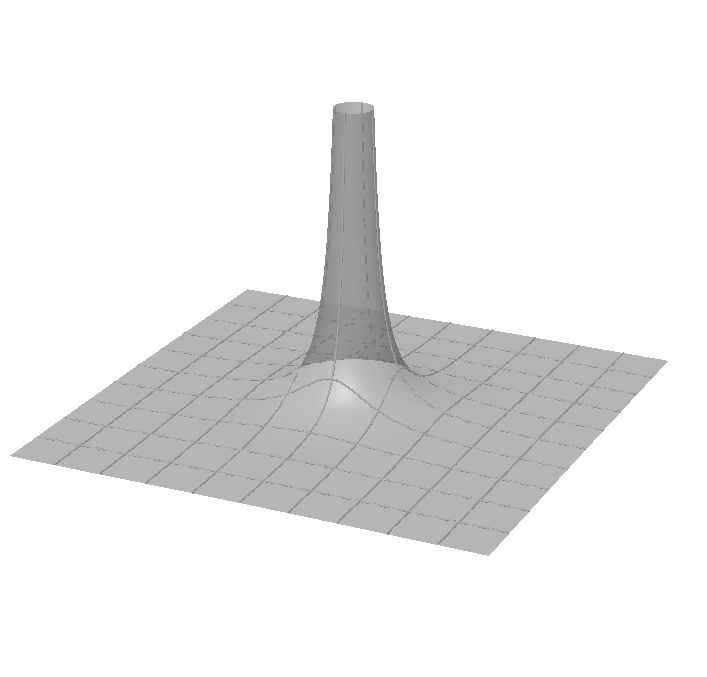
\includegraphics[width=7cm]{./media/potencial_punto.png}
  \caption{Grafica potencial un punto}
  \label{fig:potential1}
\end{figure}

\section{Desarrollo}
Pensando en la función $f_n(x,y)$\ref{eq:intuition} como una función de
potencial, podemos desarrollar el campo vectorial asociado a ella y
mediante el principio de superposición podemos obtener el campo que
dicta la tendencia a la señal transmitida.

\begin{align}
  \label{eq:development}
  F_n\left( x, y \right) &= -\nabla f_n\left( x, y \right)\\
  &= - \partder{x} f_n \left( x, y \right) \vec{i} - \partder{y} f_n \left( x, y \right) \vec{j}
\end{align}

Procedemos a derivar una función más general.

\begin{align}
  \label{eq:derivative}
  - \partder{n} f_i \left( n, m \right) &= - \partder{n} \left[ \frac{1}{\left( n - n_i \right)^2 + \left( m - m_i \right)^2 } \right]\\
  &= - \partder{n} \left( \left( n - n_i \right)^2 + \left( m - m_i \right)^2 \right)^{-1}\\
  &= - 2\left( \left( \left( n - n_i \right)^2 + \left( m - m_i \right) \right)^2 \right)^{-1} \left( n - n_i \right)\\
  &= - \frac{n - n_i}{\left( \left( n - n_i \right)^2 + \left( m - m_i \right)^2 \right)^2}
\end{align}

Caracterizando $\partder{n}f_i\left( n, m \right)$ con $n = x, m = y$ y viceversa
obtenemos el campo vectorial.

\begin{align}
  \label{eq:development2}
  F_i(x,y) = - 2 \left(
  \begin{array}{c}
    \frac{x - x_n}{\left( \left( x - x_n \right)^2 + \left( y - y_n \right)^2\right)^2}\\
    \frac{y - y_n}{\left( \left( x - x_n \right)^2 + \left( y - y_n \right)^2\right)^2}
  \end{array}
  \right)
\end{align}

Aplicando el principio de superposición, podemos obtener la siguiente fórmula,
donde $i$ representa el índice de los símbolos y $S$ el conjunto de todos los
símbolos posibles.
\begin{align}
  \label{eq:superposition}
  \vec{T_S}(x,y) = \sum\limits_{i} \vec{F_i}\left( x, y\right)
\end{align}

Si resolvemos $\vec{T_S}(x,y) = \vec{0}$, obtendremos la ecuaciones que delimitan
las regiones de decisión.

\subsection{Generalización a $\mathbb{R}^n$}
Aun que se ha desarrollado para una función $f$ de dos variables, se puede
generalizar a $f: \mathbb{R}^n \rightarrow \mathbb{R}$, donde $n$ viene dado por la dimensión de la base
del espacio de símbolos. Y $f$ se puede definir de la siguiente forma:
\begin{align}
  \label{eq:generalf}
  f(x_1, x_2, \cdots ,x_n) = \frac{1}{(x_1 - x_{1i})^2 + (x_2 - x_{2i})^2 + \cdots + (x_n - x_{ni})^2}
\end{align}
Obteniendo lo siguiente: \footnote{Este método se puede utilizar para el cálculo
de diagramas de Voronoi en $\mathbb{R}^n$ con las soluciones a $T_S = \vec{0}$}
\begin{align}
  \label{eq:generalF}
  \vec{T_S}(x_1, x_2, \cdots , x_n) &= \sum_i -\nabla f(x_1, x_2, \cdots ,x_n)
\end{align}

\section{Ejemplo}
Si consideramos dos símbolos con una base compuesta por por dos vectores
$\Phi_1$ y $\Phi_2$, con coordenadas $S_1=(x_{10}, y_{10})$ y $S_2=(x_{20}, y_{20})$, los podemos
representar en $\mathbb{R}^2$
\begin{figure}[h!]
  \centering
  % Title: gl2ps_renderer figure
% Creator: GL2PS 1.4.0, (C) 1999-2017 C. Geuzaine
% For: Octave
% CreationDate: Wed Apr 10 21:18:30 2019
\begin{pgfpicture}
\color[rgb]{1.000000,1.000000,1.000000}
\pgfpathrectanglecorners{\pgfpoint{0pt}{0pt}}{\pgfpoint{576pt}{432pt}}
\pgfusepath{fill}
\begin{pgfscope}
\pgfpathrectangle{\pgfpoint{0pt}{0pt}}{\pgfpoint{576pt}{432pt}}
\pgfusepath{fill}
\pgfpathrectangle{\pgfpoint{0pt}{0pt}}{\pgfpoint{576pt}{432pt}}
\pgfusepath{clip}
\pgfpathmoveto{\pgfpoint{74.880005pt}{399.599976pt}}
\pgflineto{\pgfpoint{521.279968pt}{47.519989pt}}
\pgflineto{\pgfpoint{74.880005pt}{47.519989pt}}
\pgfpathclose
\pgfusepath{fill,stroke}
\pgfpathmoveto{\pgfpoint{74.880005pt}{399.599976pt}}
\pgflineto{\pgfpoint{521.279968pt}{399.599976pt}}
\pgflineto{\pgfpoint{521.279968pt}{47.519989pt}}
\pgfpathclose
\pgfusepath{fill,stroke}
\color[rgb]{0.150000,0.150000,0.150000}
\pgfsetlinewidth{0.500000pt}
\pgfpathmoveto{\pgfpoint{74.880005pt}{51.985016pt}}
\pgflineto{\pgfpoint{74.880005pt}{47.519989pt}}
\pgfusepath{stroke}
\pgfpathmoveto{\pgfpoint{74.880005pt}{395.134979pt}}
\pgflineto{\pgfpoint{74.880005pt}{399.599976pt}}
\pgfusepath{stroke}
\pgfpathmoveto{\pgfpoint{186.479996pt}{51.985016pt}}
\pgflineto{\pgfpoint{186.479996pt}{47.519989pt}}
\pgfusepath{stroke}
\pgfpathmoveto{\pgfpoint{186.479996pt}{395.134979pt}}
\pgflineto{\pgfpoint{186.479996pt}{399.599976pt}}
\pgfusepath{stroke}
\pgfpathmoveto{\pgfpoint{298.079987pt}{51.985016pt}}
\pgflineto{\pgfpoint{298.079987pt}{47.519989pt}}
\pgfusepath{stroke}
\pgfpathmoveto{\pgfpoint{298.079987pt}{395.134979pt}}
\pgflineto{\pgfpoint{298.079987pt}{399.599976pt}}
\pgfusepath{stroke}
\pgfpathmoveto{\pgfpoint{409.679993pt}{51.985016pt}}
\pgflineto{\pgfpoint{409.679993pt}{47.519989pt}}
\pgfusepath{stroke}
\pgfpathmoveto{\pgfpoint{409.679993pt}{395.134979pt}}
\pgflineto{\pgfpoint{409.679993pt}{399.599976pt}}
\pgfusepath{stroke}
\pgfpathmoveto{\pgfpoint{521.279968pt}{51.985016pt}}
\pgflineto{\pgfpoint{521.279968pt}{47.519989pt}}
\pgfusepath{stroke}
\pgfpathmoveto{\pgfpoint{521.279968pt}{395.134979pt}}
\pgflineto{\pgfpoint{521.279968pt}{399.599976pt}}
\pgfusepath{stroke}
{
\pgftransformshift{\pgfpoint{74.880005pt}{40.018295pt}}
\pgfnode{rectangle}{north}{\fontsize{10}{0}\selectfont\textcolor[rgb]{0.15,0.15,0.15}{{-10}}}{}{\pgfusepath{discard}}}
{
\pgftransformshift{\pgfpoint{186.479996pt}{40.018295pt}}
\pgfnode{rectangle}{north}{\fontsize{10}{0}\selectfont\textcolor[rgb]{0.15,0.15,0.15}{{-5}}}{}{\pgfusepath{discard}}}
{
\pgftransformshift{\pgfpoint{298.079987pt}{40.018295pt}}
\pgfnode{rectangle}{north}{\fontsize{10}{0}\selectfont\textcolor[rgb]{0.15,0.15,0.15}{{0}}}{}{\pgfusepath{discard}}}
{
\pgftransformshift{\pgfpoint{409.679993pt}{40.018295pt}}
\pgfnode{rectangle}{north}{\fontsize{10}{0}\selectfont\textcolor[rgb]{0.15,0.15,0.15}{{5}}}{}{\pgfusepath{discard}}}
{
\pgftransformshift{\pgfpoint{521.279968pt}{40.018295pt}}
\pgfnode{rectangle}{north}{\fontsize{10}{0}\selectfont\textcolor[rgb]{0.15,0.15,0.15}{{10}}}{}{\pgfusepath{discard}}}
\pgfpathmoveto{\pgfpoint{79.347977pt}{47.519989pt}}
\pgflineto{\pgfpoint{74.880005pt}{47.519989pt}}
\pgfusepath{stroke}
\pgfpathmoveto{\pgfpoint{516.812012pt}{47.519989pt}}
\pgflineto{\pgfpoint{521.279968pt}{47.519989pt}}
\pgfusepath{stroke}
\pgfpathmoveto{\pgfpoint{79.347977pt}{135.539993pt}}
\pgflineto{\pgfpoint{74.880005pt}{135.539993pt}}
\pgfusepath{stroke}
\pgfpathmoveto{\pgfpoint{516.812012pt}{135.539993pt}}
\pgflineto{\pgfpoint{521.279968pt}{135.539993pt}}
\pgfusepath{stroke}
\pgfpathmoveto{\pgfpoint{79.347977pt}{223.559998pt}}
\pgflineto{\pgfpoint{74.880005pt}{223.559998pt}}
\pgfusepath{stroke}
\pgfpathmoveto{\pgfpoint{516.812012pt}{223.559998pt}}
\pgflineto{\pgfpoint{521.279968pt}{223.559998pt}}
\pgfusepath{stroke}
\pgfpathmoveto{\pgfpoint{79.347977pt}{311.579987pt}}
\pgflineto{\pgfpoint{74.880005pt}{311.579987pt}}
\pgfusepath{stroke}
\pgfpathmoveto{\pgfpoint{516.812012pt}{311.579987pt}}
\pgflineto{\pgfpoint{521.279968pt}{311.579987pt}}
\pgfusepath{stroke}
\pgfpathmoveto{\pgfpoint{79.347977pt}{399.599976pt}}
\pgflineto{\pgfpoint{74.880005pt}{399.599976pt}}
\pgfusepath{stroke}
\pgfpathmoveto{\pgfpoint{516.812012pt}{399.599976pt}}
\pgflineto{\pgfpoint{521.279968pt}{399.599976pt}}
\pgfusepath{stroke}
{
\pgftransformshift{\pgfpoint{69.875504pt}{47.519989pt}}
\pgfnode{rectangle}{east}{\fontsize{10}{0}\selectfont\textcolor[rgb]{0.15,0.15,0.15}{{-10}}}{}{\pgfusepath{discard}}}
{
\pgftransformshift{\pgfpoint{69.875504pt}{135.539993pt}}
\pgfnode{rectangle}{east}{\fontsize{10}{0}\selectfont\textcolor[rgb]{0.15,0.15,0.15}{{-5}}}{}{\pgfusepath{discard}}}
{
\pgftransformshift{\pgfpoint{69.875504pt}{223.559998pt}}
\pgfnode{rectangle}{east}{\fontsize{10}{0}\selectfont\textcolor[rgb]{0.15,0.15,0.15}{{0}}}{}{\pgfusepath{discard}}}
{
\pgftransformshift{\pgfpoint{69.875504pt}{311.579987pt}}
\pgfnode{rectangle}{east}{\fontsize{10}{0}\selectfont\textcolor[rgb]{0.15,0.15,0.15}{{5}}}{}{\pgfusepath{discard}}}
{
\pgftransformshift{\pgfpoint{69.875504pt}{399.599976pt}}
\pgfnode{rectangle}{east}{\fontsize{10}{0}\selectfont\textcolor[rgb]{0.15,0.15,0.15}{{10}}}{}{\pgfusepath{discard}}}
\pgfsetrectcap
\pgfsetdash{{16pt}{0pt}}{0pt}
\pgfpathmoveto{\pgfpoint{521.279968pt}{47.519989pt}}
\pgflineto{\pgfpoint{74.880005pt}{47.519989pt}}
\pgfusepath{stroke}
\pgfpathmoveto{\pgfpoint{521.279968pt}{399.599976pt}}
\pgflineto{\pgfpoint{74.880005pt}{399.599976pt}}
\pgfusepath{stroke}
\pgfpathmoveto{\pgfpoint{74.880005pt}{399.599976pt}}
\pgflineto{\pgfpoint{74.880005pt}{47.519989pt}}
\pgfusepath{stroke}
\pgfpathmoveto{\pgfpoint{521.279968pt}{399.599976pt}}
\pgflineto{\pgfpoint{521.279968pt}{47.519989pt}}
\pgfusepath{stroke}
\color[rgb]{0.000000,0.447000,0.741000}
\pgfsetbuttcap
\pgfsetroundjoin
\pgfsetdash{}{0pt}
\pgfpathmoveto{\pgfpoint{119.637100pt}{82.846634pt}}
\pgflineto{\pgfpoint{119.519989pt}{82.727997pt}}
\pgfusepath{stroke}
\pgfpathmoveto{\pgfpoint{119.632782pt}{89.883850pt}}
\pgflineto{\pgfpoint{119.519989pt}{89.769585pt}}
\pgfusepath{stroke}
\pgfpathmoveto{\pgfpoint{119.627960pt}{96.920517pt}}
\pgflineto{\pgfpoint{119.519989pt}{96.811195pt}}
\pgfusepath{stroke}
\pgfpathmoveto{\pgfpoint{119.622665pt}{103.956665pt}}
\pgflineto{\pgfpoint{119.519989pt}{103.852783pt}}
\pgfusepath{stroke}
\pgfpathmoveto{\pgfpoint{119.616974pt}{110.992355pt}}
\pgflineto{\pgfpoint{119.519989pt}{110.894394pt}}
\pgfusepath{stroke}
\pgfpathmoveto{\pgfpoint{119.611008pt}{118.027641pt}}
\pgflineto{\pgfpoint{119.519989pt}{117.935989pt}}
\pgfusepath{stroke}
\pgfpathmoveto{\pgfpoint{119.604889pt}{125.062599pt}}
\pgflineto{\pgfpoint{119.519989pt}{124.977592pt}}
\pgfusepath{stroke}
\pgfpathmoveto{\pgfpoint{119.598755pt}{132.097351pt}}
\pgflineto{\pgfpoint{119.519989pt}{132.019196pt}}
\pgfusepath{stroke}
\pgfpathmoveto{\pgfpoint{119.592743pt}{139.131943pt}}
\pgflineto{\pgfpoint{119.519989pt}{139.060791pt}}
\pgfusepath{stroke}
\pgfpathmoveto{\pgfpoint{119.587036pt}{146.166534pt}}
\pgflineto{\pgfpoint{119.519989pt}{146.102386pt}}
\pgfusepath{stroke}
\pgfpathmoveto{\pgfpoint{119.581757pt}{153.201157pt}}
\pgflineto{\pgfpoint{119.519989pt}{153.143997pt}}
\pgfusepath{stroke}
\pgfpathmoveto{\pgfpoint{119.577072pt}{160.235931pt}}
\pgflineto{\pgfpoint{119.519989pt}{160.185593pt}}
\pgfusepath{stroke}
\pgfpathmoveto{\pgfpoint{119.573059pt}{167.270920pt}}
\pgflineto{\pgfpoint{119.519989pt}{167.227188pt}}
\pgfusepath{stroke}
\pgfpathmoveto{\pgfpoint{119.569855pt}{174.306168pt}}
\pgflineto{\pgfpoint{119.519989pt}{174.268799pt}}
\pgfusepath{stroke}
\pgfpathmoveto{\pgfpoint{119.567535pt}{181.341705pt}}
\pgflineto{\pgfpoint{119.519989pt}{181.310394pt}}
\pgfusepath{stroke}
\pgfpathmoveto{\pgfpoint{119.566101pt}{188.377533pt}}
\pgflineto{\pgfpoint{119.519989pt}{188.351990pt}}
\pgfusepath{stroke}
\pgfpathmoveto{\pgfpoint{119.565598pt}{195.413635pt}}
\pgflineto{\pgfpoint{119.519989pt}{195.393585pt}}
\pgfusepath{stroke}
\pgfpathmoveto{\pgfpoint{119.566025pt}{202.449982pt}}
\pgflineto{\pgfpoint{119.519989pt}{202.435196pt}}
\pgfusepath{stroke}
\pgfpathmoveto{\pgfpoint{119.567322pt}{209.486542pt}}
\pgflineto{\pgfpoint{119.519989pt}{209.476791pt}}
\pgfusepath{stroke}
\pgfpathmoveto{\pgfpoint{119.569443pt}{216.523224pt}}
\pgflineto{\pgfpoint{119.519989pt}{216.518387pt}}
\pgfusepath{stroke}
\pgfpathmoveto{\pgfpoint{119.572327pt}{223.559998pt}}
\pgflineto{\pgfpoint{119.519989pt}{223.559998pt}}
\pgfusepath{stroke}
\pgfpathmoveto{\pgfpoint{119.575851pt}{230.596756pt}}
\pgflineto{\pgfpoint{119.519989pt}{230.601593pt}}
\pgfusepath{stroke}
\pgfpathmoveto{\pgfpoint{119.579895pt}{237.633453pt}}
\pgflineto{\pgfpoint{119.519989pt}{237.643188pt}}
\pgfusepath{stroke}
\pgfpathmoveto{\pgfpoint{119.584366pt}{244.669998pt}}
\pgflineto{\pgfpoint{119.519989pt}{244.684799pt}}
\pgfusepath{stroke}
\pgfpathmoveto{\pgfpoint{119.589096pt}{251.706360pt}}
\pgflineto{\pgfpoint{119.519989pt}{251.726395pt}}
\pgfusepath{stroke}
\pgfpathmoveto{\pgfpoint{119.593964pt}{258.742462pt}}
\pgflineto{\pgfpoint{119.519989pt}{258.768005pt}}
\pgfusepath{stroke}
\pgfpathmoveto{\pgfpoint{119.598785pt}{265.778290pt}}
\pgflineto{\pgfpoint{119.519989pt}{265.809601pt}}
\pgfusepath{stroke}
\pgfpathmoveto{\pgfpoint{119.603424pt}{272.813812pt}}
\pgflineto{\pgfpoint{119.519989pt}{272.851196pt}}
\pgfusepath{stroke}
\pgfpathmoveto{\pgfpoint{119.607697pt}{279.849060pt}}
\pgflineto{\pgfpoint{119.519989pt}{279.892792pt}}
\pgfusepath{stroke}
\pgfpathmoveto{\pgfpoint{119.611496pt}{286.884033pt}}
\pgflineto{\pgfpoint{119.519989pt}{286.934387pt}}
\pgfusepath{stroke}
\pgfpathmoveto{\pgfpoint{119.614716pt}{293.918823pt}}
\pgflineto{\pgfpoint{119.519989pt}{293.975983pt}}
\pgfusepath{stroke}
\pgfpathmoveto{\pgfpoint{119.617188pt}{300.953461pt}}
\pgflineto{\pgfpoint{119.519989pt}{301.017578pt}}
\pgfusepath{stroke}
\pgfpathmoveto{\pgfpoint{119.618866pt}{307.988037pt}}
\pgflineto{\pgfpoint{119.519989pt}{308.059204pt}}
\pgfusepath{stroke}
\pgfpathmoveto{\pgfpoint{119.619690pt}{315.022644pt}}
\pgflineto{\pgfpoint{119.519989pt}{315.100800pt}}
\pgfusepath{stroke}
\pgfpathmoveto{\pgfpoint{119.619659pt}{322.057373pt}}
\pgflineto{\pgfpoint{119.519989pt}{322.142395pt}}
\pgfusepath{stroke}
\pgfpathmoveto{\pgfpoint{119.618759pt}{329.092346pt}}
\pgflineto{\pgfpoint{119.519989pt}{329.183990pt}}
\pgfusepath{stroke}
\pgfpathmoveto{\pgfpoint{119.617050pt}{336.127625pt}}
\pgflineto{\pgfpoint{119.519989pt}{336.225586pt}}
\pgfusepath{stroke}
\pgfpathmoveto{\pgfpoint{119.614563pt}{343.163330pt}}
\pgflineto{\pgfpoint{119.519989pt}{343.267212pt}}
\pgfusepath{stroke}
\pgfpathmoveto{\pgfpoint{119.611420pt}{350.199463pt}}
\pgflineto{\pgfpoint{119.519989pt}{350.308777pt}}
\pgfusepath{stroke}
\pgfpathmoveto{\pgfpoint{119.607697pt}{357.236145pt}}
\pgflineto{\pgfpoint{119.519989pt}{357.350403pt}}
\pgfusepath{stroke}
\pgfpathmoveto{\pgfpoint{119.603500pt}{364.273376pt}}
\pgflineto{\pgfpoint{119.519989pt}{364.391998pt}}
\pgfusepath{stroke}
\pgfpathmoveto{\pgfpoint{128.569794pt}{82.853226pt}}
\pgflineto{\pgfpoint{128.447998pt}{82.727997pt}}
\pgfusepath{stroke}
\pgfpathmoveto{\pgfpoint{128.565048pt}{89.890198pt}}
\pgflineto{\pgfpoint{128.447998pt}{89.769585pt}}
\pgfusepath{stroke}
\pgfpathmoveto{\pgfpoint{128.559662pt}{96.926529pt}}
\pgflineto{\pgfpoint{128.447998pt}{96.811195pt}}
\pgfusepath{stroke}
\pgfpathmoveto{\pgfpoint{128.553711pt}{103.962280pt}}
\pgflineto{\pgfpoint{128.447998pt}{103.852783pt}}
\pgfusepath{stroke}
\pgfpathmoveto{\pgfpoint{128.547226pt}{110.997467pt}}
\pgflineto{\pgfpoint{128.447998pt}{110.894394pt}}
\pgfusepath{stroke}
\pgfpathmoveto{\pgfpoint{128.540421pt}{118.032181pt}}
\pgflineto{\pgfpoint{128.447998pt}{117.935989pt}}
\pgfusepath{stroke}
\pgfpathmoveto{\pgfpoint{128.533386pt}{125.066528pt}}
\pgflineto{\pgfpoint{128.447998pt}{124.977592pt}}
\pgfusepath{stroke}
\pgfpathmoveto{\pgfpoint{128.526291pt}{132.100616pt}}
\pgflineto{\pgfpoint{128.447998pt}{132.019196pt}}
\pgfusepath{stroke}
\pgfpathmoveto{\pgfpoint{128.519333pt}{139.134583pt}}
\pgflineto{\pgfpoint{128.447998pt}{139.060791pt}}
\pgfusepath{stroke}
\pgfpathmoveto{\pgfpoint{128.512711pt}{146.168518pt}}
\pgflineto{\pgfpoint{128.447998pt}{146.102386pt}}
\pgfusepath{stroke}
\pgfpathmoveto{\pgfpoint{128.506592pt}{153.202576pt}}
\pgflineto{\pgfpoint{128.447998pt}{153.143997pt}}
\pgfusepath{stroke}
\pgfpathmoveto{\pgfpoint{128.501175pt}{160.236832pt}}
\pgflineto{\pgfpoint{128.447998pt}{160.185593pt}}
\pgfusepath{stroke}
\pgfpathmoveto{\pgfpoint{128.496582pt}{167.271393pt}}
\pgflineto{\pgfpoint{128.447998pt}{167.227188pt}}
\pgfusepath{stroke}
\pgfpathmoveto{\pgfpoint{128.492920pt}{174.306290pt}}
\pgflineto{\pgfpoint{128.447998pt}{174.268799pt}}
\pgfusepath{stroke}
\pgfpathmoveto{\pgfpoint{128.490295pt}{181.341583pt}}
\pgflineto{\pgfpoint{128.447998pt}{181.310394pt}}
\pgfusepath{stroke}
\pgfpathmoveto{\pgfpoint{128.488739pt}{188.377258pt}}
\pgflineto{\pgfpoint{128.447998pt}{188.351990pt}}
\pgfusepath{stroke}
\pgfpathmoveto{\pgfpoint{128.488297pt}{195.413300pt}}
\pgflineto{\pgfpoint{128.447998pt}{195.393585pt}}
\pgfusepath{stroke}
\pgfpathmoveto{\pgfpoint{128.488937pt}{202.449661pt}}
\pgflineto{\pgfpoint{128.447998pt}{202.435196pt}}
\pgfusepath{stroke}
\pgfpathmoveto{\pgfpoint{128.490601pt}{209.486282pt}}
\pgflineto{\pgfpoint{128.447998pt}{209.476791pt}}
\pgfusepath{stroke}
\pgfpathmoveto{\pgfpoint{128.493240pt}{216.523087pt}}
\pgflineto{\pgfpoint{128.447998pt}{216.518387pt}}
\pgfusepath{stroke}
\pgfpathmoveto{\pgfpoint{128.496765pt}{223.559998pt}}
\pgflineto{\pgfpoint{128.447998pt}{223.559998pt}}
\pgfusepath{stroke}
\pgfpathmoveto{\pgfpoint{128.501053pt}{230.596893pt}}
\pgflineto{\pgfpoint{128.447998pt}{230.601593pt}}
\pgfusepath{stroke}
\pgfpathmoveto{\pgfpoint{128.505966pt}{237.633698pt}}
\pgflineto{\pgfpoint{128.447998pt}{237.643188pt}}
\pgfusepath{stroke}
\pgfpathmoveto{\pgfpoint{128.511353pt}{244.670319pt}}
\pgflineto{\pgfpoint{128.447998pt}{244.684799pt}}
\pgfusepath{stroke}
\pgfpathmoveto{\pgfpoint{128.517075pt}{251.706696pt}}
\pgflineto{\pgfpoint{128.447998pt}{251.726395pt}}
\pgfusepath{stroke}
\pgfpathmoveto{\pgfpoint{128.522949pt}{258.742737pt}}
\pgflineto{\pgfpoint{128.447998pt}{258.768005pt}}
\pgfusepath{stroke}
\pgfpathmoveto{\pgfpoint{128.528763pt}{265.778412pt}}
\pgflineto{\pgfpoint{128.447998pt}{265.809601pt}}
\pgfusepath{stroke}
\pgfpathmoveto{\pgfpoint{128.534378pt}{272.813690pt}}
\pgflineto{\pgfpoint{128.447998pt}{272.851196pt}}
\pgfusepath{stroke}
\pgfpathmoveto{\pgfpoint{128.539581pt}{279.848602pt}}
\pgflineto{\pgfpoint{128.447998pt}{279.892792pt}}
\pgfusepath{stroke}
\pgfpathmoveto{\pgfpoint{128.544205pt}{286.883148pt}}
\pgflineto{\pgfpoint{128.447998pt}{286.934387pt}}
\pgfusepath{stroke}
\pgfpathmoveto{\pgfpoint{128.548111pt}{293.917419pt}}
\pgflineto{\pgfpoint{128.447998pt}{293.975983pt}}
\pgfusepath{stroke}
\pgfpathmoveto{\pgfpoint{128.551132pt}{300.951477pt}}
\pgflineto{\pgfpoint{128.447998pt}{301.017578pt}}
\pgfusepath{stroke}
\pgfpathmoveto{\pgfpoint{128.553207pt}{307.985413pt}}
\pgflineto{\pgfpoint{128.447998pt}{308.059204pt}}
\pgfusepath{stroke}
\pgfpathmoveto{\pgfpoint{128.554276pt}{315.019348pt}}
\pgflineto{\pgfpoint{128.447998pt}{315.100800pt}}
\pgfusepath{stroke}
\pgfpathmoveto{\pgfpoint{128.554276pt}{322.053467pt}}
\pgflineto{\pgfpoint{128.447998pt}{322.142395pt}}
\pgfusepath{stroke}
\pgfpathmoveto{\pgfpoint{128.553253pt}{329.087830pt}}
\pgflineto{\pgfpoint{128.447998pt}{329.183990pt}}
\pgfusepath{stroke}
\pgfpathmoveto{\pgfpoint{128.551285pt}{336.122528pt}}
\pgflineto{\pgfpoint{128.447998pt}{336.225586pt}}
\pgfusepath{stroke}
\pgfpathmoveto{\pgfpoint{128.548431pt}{343.157715pt}}
\pgflineto{\pgfpoint{128.447998pt}{343.267212pt}}
\pgfusepath{stroke}
\pgfpathmoveto{\pgfpoint{128.544800pt}{350.193451pt}}
\pgflineto{\pgfpoint{128.447998pt}{350.308777pt}}
\pgfusepath{stroke}
\pgfpathmoveto{\pgfpoint{128.540527pt}{357.229797pt}}
\pgflineto{\pgfpoint{128.447998pt}{357.350403pt}}
\pgfusepath{stroke}
\pgfpathmoveto{\pgfpoint{128.535706pt}{364.266785pt}}
\pgflineto{\pgfpoint{128.447998pt}{364.391998pt}}
\pgfusepath{stroke}
\pgfpathmoveto{\pgfpoint{137.503174pt}{82.860458pt}}
\pgflineto{\pgfpoint{137.376007pt}{82.727997pt}}
\pgfusepath{stroke}
\pgfpathmoveto{\pgfpoint{137.497955pt}{89.897186pt}}
\pgflineto{\pgfpoint{137.376007pt}{89.769585pt}}
\pgfusepath{stroke}
\pgfpathmoveto{\pgfpoint{137.491959pt}{96.933159pt}}
\pgflineto{\pgfpoint{137.376007pt}{96.811195pt}}
\pgfusepath{stroke}
\pgfpathmoveto{\pgfpoint{137.485229pt}{103.968422pt}}
\pgflineto{\pgfpoint{137.376007pt}{103.852783pt}}
\pgfusepath{stroke}
\pgfpathmoveto{\pgfpoint{137.477875pt}{111.003036pt}}
\pgflineto{\pgfpoint{137.376007pt}{110.894394pt}}
\pgfusepath{stroke}
\pgfpathmoveto{\pgfpoint{137.470047pt}{118.037102pt}}
\pgflineto{\pgfpoint{137.376007pt}{117.935989pt}}
\pgfusepath{stroke}
\pgfpathmoveto{\pgfpoint{137.461914pt}{125.070717pt}}
\pgflineto{\pgfpoint{137.376007pt}{124.977592pt}}
\pgfusepath{stroke}
\pgfpathmoveto{\pgfpoint{137.453690pt}{132.104034pt}}
\pgflineto{\pgfpoint{137.376007pt}{132.019196pt}}
\pgfusepath{stroke}
\pgfpathmoveto{\pgfpoint{137.445587pt}{139.137207pt}}
\pgflineto{\pgfpoint{137.376007pt}{139.060791pt}}
\pgfusepath{stroke}
\pgfpathmoveto{\pgfpoint{137.437866pt}{146.170410pt}}
\pgflineto{\pgfpoint{137.376007pt}{146.102386pt}}
\pgfusepath{stroke}
\pgfpathmoveto{\pgfpoint{137.430756pt}{153.203781pt}}
\pgflineto{\pgfpoint{137.376007pt}{153.143997pt}}
\pgfusepath{stroke}
\pgfpathmoveto{\pgfpoint{137.424454pt}{160.237427pt}}
\pgflineto{\pgfpoint{137.376007pt}{160.185593pt}}
\pgfusepath{stroke}
\pgfpathmoveto{\pgfpoint{137.419144pt}{167.271484pt}}
\pgflineto{\pgfpoint{137.376007pt}{167.227188pt}}
\pgfusepath{stroke}
\pgfpathmoveto{\pgfpoint{137.414932pt}{174.306030pt}}
\pgflineto{\pgfpoint{137.376007pt}{174.268799pt}}
\pgfusepath{stroke}
\pgfpathmoveto{\pgfpoint{137.411957pt}{181.341064pt}}
\pgflineto{\pgfpoint{137.376007pt}{181.310394pt}}
\pgfusepath{stroke}
\pgfpathmoveto{\pgfpoint{137.410278pt}{188.376617pt}}
\pgflineto{\pgfpoint{137.376007pt}{188.351990pt}}
\pgfusepath{stroke}
\pgfpathmoveto{\pgfpoint{137.409897pt}{195.412643pt}}
\pgflineto{\pgfpoint{137.376007pt}{195.393585pt}}
\pgfusepath{stroke}
\pgfpathmoveto{\pgfpoint{137.410797pt}{202.449081pt}}
\pgflineto{\pgfpoint{137.376007pt}{202.435196pt}}
\pgfusepath{stroke}
\pgfpathmoveto{\pgfpoint{137.412903pt}{209.485855pt}}
\pgflineto{\pgfpoint{137.376007pt}{209.476791pt}}
\pgfusepath{stroke}
\pgfpathmoveto{\pgfpoint{137.416168pt}{216.522873pt}}
\pgflineto{\pgfpoint{137.376007pt}{216.518387pt}}
\pgfusepath{stroke}
\pgfpathmoveto{\pgfpoint{137.420441pt}{223.559998pt}}
\pgflineto{\pgfpoint{137.376007pt}{223.559998pt}}
\pgfusepath{stroke}
\pgfpathmoveto{\pgfpoint{137.425613pt}{230.597122pt}}
\pgflineto{\pgfpoint{137.376007pt}{230.601593pt}}
\pgfusepath{stroke}
\pgfpathmoveto{\pgfpoint{137.431534pt}{237.634125pt}}
\pgflineto{\pgfpoint{137.376007pt}{237.643188pt}}
\pgfusepath{stroke}
\pgfpathmoveto{\pgfpoint{137.438019pt}{244.670898pt}}
\pgflineto{\pgfpoint{137.376007pt}{244.684799pt}}
\pgfusepath{stroke}
\pgfpathmoveto{\pgfpoint{137.444901pt}{251.707352pt}}
\pgflineto{\pgfpoint{137.376007pt}{251.726395pt}}
\pgfusepath{stroke}
\pgfpathmoveto{\pgfpoint{137.451965pt}{258.743378pt}}
\pgflineto{\pgfpoint{137.376007pt}{258.768005pt}}
\pgfusepath{stroke}
\pgfpathmoveto{\pgfpoint{137.458969pt}{265.778931pt}}
\pgflineto{\pgfpoint{137.376007pt}{265.809601pt}}
\pgfusepath{stroke}
\pgfpathmoveto{\pgfpoint{137.465729pt}{272.813965pt}}
\pgflineto{\pgfpoint{137.376007pt}{272.851196pt}}
\pgfusepath{stroke}
\pgfpathmoveto{\pgfpoint{137.472031pt}{279.848480pt}}
\pgflineto{\pgfpoint{137.376007pt}{279.892792pt}}
\pgfusepath{stroke}
\pgfpathmoveto{\pgfpoint{137.477646pt}{286.882568pt}}
\pgflineto{\pgfpoint{137.376007pt}{286.934387pt}}
\pgfusepath{stroke}
\pgfpathmoveto{\pgfpoint{137.482346pt}{293.916199pt}}
\pgflineto{\pgfpoint{137.376007pt}{293.975983pt}}
\pgfusepath{stroke}
\pgfpathmoveto{\pgfpoint{137.486038pt}{300.949585pt}}
\pgflineto{\pgfpoint{137.376007pt}{301.017578pt}}
\pgfusepath{stroke}
\pgfpathmoveto{\pgfpoint{137.488556pt}{307.982788pt}}
\pgflineto{\pgfpoint{137.376007pt}{308.059204pt}}
\pgfusepath{stroke}
\pgfpathmoveto{\pgfpoint{137.489868pt}{315.015930pt}}
\pgflineto{\pgfpoint{137.376007pt}{315.100800pt}}
\pgfusepath{stroke}
\pgfpathmoveto{\pgfpoint{137.489914pt}{322.049255pt}}
\pgflineto{\pgfpoint{137.376007pt}{322.142395pt}}
\pgfusepath{stroke}
\pgfpathmoveto{\pgfpoint{137.488724pt}{329.082886pt}}
\pgflineto{\pgfpoint{137.376007pt}{329.183990pt}}
\pgfusepath{stroke}
\pgfpathmoveto{\pgfpoint{137.486420pt}{336.116943pt}}
\pgflineto{\pgfpoint{137.376007pt}{336.225586pt}}
\pgfusepath{stroke}
\pgfpathmoveto{\pgfpoint{137.483063pt}{343.151550pt}}
\pgflineto{\pgfpoint{137.376007pt}{343.267212pt}}
\pgfusepath{stroke}
\pgfpathmoveto{\pgfpoint{137.478821pt}{350.186829pt}}
\pgflineto{\pgfpoint{137.376007pt}{350.308777pt}}
\pgfusepath{stroke}
\pgfpathmoveto{\pgfpoint{137.473862pt}{357.222778pt}}
\pgflineto{\pgfpoint{137.376007pt}{357.350403pt}}
\pgfusepath{stroke}
\pgfpathmoveto{\pgfpoint{137.468338pt}{364.259521pt}}
\pgflineto{\pgfpoint{137.376007pt}{364.391998pt}}
\pgfusepath{stroke}
\pgfpathmoveto{\pgfpoint{146.437347pt}{82.868454pt}}
\pgflineto{\pgfpoint{146.303986pt}{82.727997pt}}
\pgfusepath{stroke}
\pgfpathmoveto{\pgfpoint{146.431656pt}{89.904922pt}}
\pgflineto{\pgfpoint{146.303986pt}{89.769585pt}}
\pgfusepath{stroke}
\pgfpathmoveto{\pgfpoint{146.424973pt}{96.940506pt}}
\pgflineto{\pgfpoint{146.303986pt}{96.811195pt}}
\pgfusepath{stroke}
\pgfpathmoveto{\pgfpoint{146.417389pt}{103.975235pt}}
\pgflineto{\pgfpoint{146.303986pt}{103.852783pt}}
\pgfusepath{stroke}
\pgfpathmoveto{\pgfpoint{146.408997pt}{111.009178pt}}
\pgflineto{\pgfpoint{146.303986pt}{110.894394pt}}
\pgfusepath{stroke}
\pgfpathmoveto{\pgfpoint{146.399979pt}{118.042458pt}}
\pgflineto{\pgfpoint{146.303986pt}{117.935989pt}}
\pgfusepath{stroke}
\pgfpathmoveto{\pgfpoint{146.390533pt}{125.075203pt}}
\pgflineto{\pgfpoint{146.303986pt}{124.977592pt}}
\pgfusepath{stroke}
\pgfpathmoveto{\pgfpoint{146.380951pt}{132.107590pt}}
\pgflineto{\pgfpoint{146.303986pt}{132.019196pt}}
\pgfusepath{stroke}
\pgfpathmoveto{\pgfpoint{146.371490pt}{139.139847pt}}
\pgflineto{\pgfpoint{146.303986pt}{139.060791pt}}
\pgfusepath{stroke}
\pgfpathmoveto{\pgfpoint{146.362442pt}{146.172134pt}}
\pgflineto{\pgfpoint{146.303986pt}{146.102386pt}}
\pgfusepath{stroke}
\pgfpathmoveto{\pgfpoint{146.354095pt}{153.204681pt}}
\pgflineto{\pgfpoint{146.303986pt}{153.143997pt}}
\pgfusepath{stroke}
\pgfpathmoveto{\pgfpoint{146.346725pt}{160.237640pt}}
\pgflineto{\pgfpoint{146.303986pt}{160.185593pt}}
\pgfusepath{stroke}
\pgfpathmoveto{\pgfpoint{146.340546pt}{167.271133pt}}
\pgflineto{\pgfpoint{146.303986pt}{167.227188pt}}
\pgfusepath{stroke}
\pgfpathmoveto{\pgfpoint{146.335709pt}{174.305252pt}}
\pgflineto{\pgfpoint{146.303986pt}{174.268799pt}}
\pgfusepath{stroke}
\pgfpathmoveto{\pgfpoint{146.332367pt}{181.340042pt}}
\pgflineto{\pgfpoint{146.303986pt}{181.310394pt}}
\pgfusepath{stroke}
\pgfpathmoveto{\pgfpoint{146.330521pt}{188.375488pt}}
\pgflineto{\pgfpoint{146.303986pt}{188.351990pt}}
\pgfusepath{stroke}
\pgfpathmoveto{\pgfpoint{146.330231pt}{195.411560pt}}
\pgflineto{\pgfpoint{146.303986pt}{195.393585pt}}
\pgfusepath{stroke}
\pgfpathmoveto{\pgfpoint{146.331436pt}{202.448166pt}}
\pgflineto{\pgfpoint{146.303986pt}{202.435196pt}}
\pgfusepath{stroke}
\pgfpathmoveto{\pgfpoint{146.334076pt}{209.485199pt}}
\pgflineto{\pgfpoint{146.303986pt}{209.476791pt}}
\pgfusepath{stroke}
\pgfpathmoveto{\pgfpoint{146.338043pt}{216.522522pt}}
\pgflineto{\pgfpoint{146.303986pt}{216.518387pt}}
\pgfusepath{stroke}
\pgfpathmoveto{\pgfpoint{146.343216pt}{223.559998pt}}
\pgflineto{\pgfpoint{146.303986pt}{223.559998pt}}
\pgfusepath{stroke}
\pgfpathmoveto{\pgfpoint{146.349426pt}{230.597473pt}}
\pgflineto{\pgfpoint{146.303986pt}{230.601593pt}}
\pgfusepath{stroke}
\pgfpathmoveto{\pgfpoint{146.356537pt}{237.634796pt}}
\pgflineto{\pgfpoint{146.303986pt}{237.643188pt}}
\pgfusepath{stroke}
\pgfpathmoveto{\pgfpoint{146.364288pt}{244.671814pt}}
\pgflineto{\pgfpoint{146.303986pt}{244.684799pt}}
\pgfusepath{stroke}
\pgfpathmoveto{\pgfpoint{146.372528pt}{251.708435pt}}
\pgflineto{\pgfpoint{146.303986pt}{251.726395pt}}
\pgfusepath{stroke}
\pgfpathmoveto{\pgfpoint{146.380997pt}{258.744507pt}}
\pgflineto{\pgfpoint{146.303986pt}{258.768005pt}}
\pgfusepath{stroke}
\pgfpathmoveto{\pgfpoint{146.389435pt}{265.779938pt}}
\pgflineto{\pgfpoint{146.303986pt}{265.809601pt}}
\pgfusepath{stroke}
\pgfpathmoveto{\pgfpoint{146.397583pt}{272.814728pt}}
\pgflineto{\pgfpoint{146.303986pt}{272.851196pt}}
\pgfusepath{stroke}
\pgfpathmoveto{\pgfpoint{146.405167pt}{279.848846pt}}
\pgflineto{\pgfpoint{146.303986pt}{279.892792pt}}
\pgfusepath{stroke}
\pgfpathmoveto{\pgfpoint{146.411942pt}{286.882355pt}}
\pgflineto{\pgfpoint{146.303986pt}{286.934387pt}}
\pgfusepath{stroke}
\pgfpathmoveto{\pgfpoint{146.417648pt}{293.915314pt}}
\pgflineto{\pgfpoint{146.303986pt}{293.975983pt}}
\pgfusepath{stroke}
\pgfpathmoveto{\pgfpoint{146.422104pt}{300.947845pt}}
\pgflineto{\pgfpoint{146.303986pt}{301.017578pt}}
\pgfusepath{stroke}
\pgfpathmoveto{\pgfpoint{146.425171pt}{307.980133pt}}
\pgflineto{\pgfpoint{146.303986pt}{308.059204pt}}
\pgfusepath{stroke}
\pgfpathmoveto{\pgfpoint{146.426727pt}{315.012390pt}}
\pgflineto{\pgfpoint{146.303986pt}{315.100800pt}}
\pgfusepath{stroke}
\pgfpathmoveto{\pgfpoint{146.426773pt}{322.044800pt}}
\pgflineto{\pgfpoint{146.303986pt}{322.142395pt}}
\pgfusepath{stroke}
\pgfpathmoveto{\pgfpoint{146.425354pt}{329.077545pt}}
\pgflineto{\pgfpoint{146.303986pt}{329.183990pt}}
\pgfusepath{stroke}
\pgfpathmoveto{\pgfpoint{146.422577pt}{336.110809pt}}
\pgflineto{\pgfpoint{146.303986pt}{336.225586pt}}
\pgfusepath{stroke}
\pgfpathmoveto{\pgfpoint{146.418594pt}{343.144745pt}}
\pgflineto{\pgfpoint{146.303986pt}{343.267212pt}}
\pgfusepath{stroke}
\pgfpathmoveto{\pgfpoint{146.413574pt}{350.179474pt}}
\pgflineto{\pgfpoint{146.303986pt}{350.308777pt}}
\pgfusepath{stroke}
\pgfpathmoveto{\pgfpoint{146.407761pt}{357.215057pt}}
\pgflineto{\pgfpoint{146.303986pt}{357.350403pt}}
\pgfusepath{stroke}
\pgfpathmoveto{\pgfpoint{146.401337pt}{364.251526pt}}
\pgflineto{\pgfpoint{146.303986pt}{364.391998pt}}
\pgfusepath{stroke}
\pgfpathmoveto{\pgfpoint{155.372543pt}{82.877335pt}}
\pgflineto{\pgfpoint{155.231979pt}{82.727997pt}}
\pgfusepath{stroke}
\pgfpathmoveto{\pgfpoint{155.366333pt}{89.913567pt}}
\pgflineto{\pgfpoint{155.231979pt}{89.769585pt}}
\pgfusepath{stroke}
\pgfpathmoveto{\pgfpoint{155.358917pt}{96.948708pt}}
\pgflineto{\pgfpoint{155.231979pt}{96.811195pt}}
\pgfusepath{stroke}
\pgfpathmoveto{\pgfpoint{155.350357pt}{103.982841pt}}
\pgflineto{\pgfpoint{155.231979pt}{103.852783pt}}
\pgfusepath{stroke}
\pgfpathmoveto{\pgfpoint{155.340759pt}{111.016006pt}}
\pgflineto{\pgfpoint{155.231979pt}{110.894394pt}}
\pgfusepath{stroke}
\pgfpathmoveto{\pgfpoint{155.330338pt}{118.048340pt}}
\pgflineto{\pgfpoint{155.231979pt}{117.935989pt}}
\pgfusepath{stroke}
\pgfpathmoveto{\pgfpoint{155.319336pt}{125.080025pt}}
\pgflineto{\pgfpoint{155.231979pt}{124.977592pt}}
\pgfusepath{stroke}
\pgfpathmoveto{\pgfpoint{155.308075pt}{132.111298pt}}
\pgflineto{\pgfpoint{155.231979pt}{132.019196pt}}
\pgfusepath{stroke}
\pgfpathmoveto{\pgfpoint{155.296936pt}{139.142426pt}}
\pgflineto{\pgfpoint{155.231979pt}{139.060791pt}}
\pgfusepath{stroke}
\pgfpathmoveto{\pgfpoint{155.286285pt}{146.173615pt}}
\pgflineto{\pgfpoint{155.231979pt}{146.102386pt}}
\pgfusepath{stroke}
\pgfpathmoveto{\pgfpoint{155.276459pt}{153.205170pt}}
\pgflineto{\pgfpoint{155.231979pt}{153.143997pt}}
\pgfusepath{stroke}
\pgfpathmoveto{\pgfpoint{155.267807pt}{160.237289pt}}
\pgflineto{\pgfpoint{155.231979pt}{160.185593pt}}
\pgfusepath{stroke}
\pgfpathmoveto{\pgfpoint{155.260590pt}{167.270126pt}}
\pgflineto{\pgfpoint{155.231979pt}{167.227188pt}}
\pgfusepath{stroke}
\pgfpathmoveto{\pgfpoint{155.255020pt}{174.303802pt}}
\pgflineto{\pgfpoint{155.231979pt}{174.268799pt}}
\pgfusepath{stroke}
\pgfpathmoveto{\pgfpoint{155.251205pt}{181.338348pt}}
\pgflineto{\pgfpoint{155.231979pt}{181.310394pt}}
\pgfusepath{stroke}
\pgfpathmoveto{\pgfpoint{155.249222pt}{188.373749pt}}
\pgflineto{\pgfpoint{155.231979pt}{188.351990pt}}
\pgfusepath{stroke}
\pgfpathmoveto{\pgfpoint{155.249054pt}{195.409943pt}}
\pgflineto{\pgfpoint{155.231979pt}{195.393585pt}}
\pgfusepath{stroke}
\pgfpathmoveto{\pgfpoint{155.250641pt}{202.446823pt}}
\pgflineto{\pgfpoint{155.231979pt}{202.435196pt}}
\pgfusepath{stroke}
\pgfpathmoveto{\pgfpoint{155.253906pt}{209.484238pt}}
\pgflineto{\pgfpoint{155.231979pt}{209.476791pt}}
\pgfusepath{stroke}
\pgfpathmoveto{\pgfpoint{155.258728pt}{216.522018pt}}
\pgflineto{\pgfpoint{155.231979pt}{216.518387pt}}
\pgfusepath{stroke}
\pgfpathmoveto{\pgfpoint{155.264938pt}{223.559998pt}}
\pgflineto{\pgfpoint{155.231979pt}{223.559998pt}}
\pgfusepath{stroke}
\pgfpathmoveto{\pgfpoint{155.272369pt}{230.597961pt}}
\pgflineto{\pgfpoint{155.231979pt}{230.601593pt}}
\pgfusepath{stroke}
\pgfpathmoveto{\pgfpoint{155.280838pt}{237.635757pt}}
\pgflineto{\pgfpoint{155.231979pt}{237.643188pt}}
\pgfusepath{stroke}
\pgfpathmoveto{\pgfpoint{155.290115pt}{244.673172pt}}
\pgflineto{\pgfpoint{155.231979pt}{244.684799pt}}
\pgfusepath{stroke}
\pgfpathmoveto{\pgfpoint{155.299942pt}{251.710052pt}}
\pgflineto{\pgfpoint{155.231979pt}{251.726395pt}}
\pgfusepath{stroke}
\pgfpathmoveto{\pgfpoint{155.310059pt}{258.746246pt}}
\pgflineto{\pgfpoint{155.231979pt}{258.768005pt}}
\pgfusepath{stroke}
\pgfpathmoveto{\pgfpoint{155.320190pt}{265.781647pt}}
\pgflineto{\pgfpoint{155.231979pt}{265.809601pt}}
\pgfusepath{stroke}
\pgfpathmoveto{\pgfpoint{155.329971pt}{272.816193pt}}
\pgflineto{\pgfpoint{155.231979pt}{272.851196pt}}
\pgfusepath{stroke}
\pgfpathmoveto{\pgfpoint{155.339127pt}{279.849854pt}}
\pgflineto{\pgfpoint{155.231979pt}{279.892792pt}}
\pgfusepath{stroke}
\pgfpathmoveto{\pgfpoint{155.347321pt}{286.882690pt}}
\pgflineto{\pgfpoint{155.231979pt}{286.934387pt}}
\pgfusepath{stroke}
\pgfpathmoveto{\pgfpoint{155.354218pt}{293.914795pt}}
\pgflineto{\pgfpoint{155.231979pt}{293.975983pt}}
\pgfusepath{stroke}
\pgfpathmoveto{\pgfpoint{155.359604pt}{300.946350pt}}
\pgflineto{\pgfpoint{155.231979pt}{301.017578pt}}
\pgfusepath{stroke}
\pgfpathmoveto{\pgfpoint{155.363281pt}{307.977570pt}}
\pgflineto{\pgfpoint{155.231979pt}{308.059204pt}}
\pgfusepath{stroke}
\pgfpathmoveto{\pgfpoint{155.365128pt}{315.008667pt}}
\pgflineto{\pgfpoint{155.231979pt}{315.100800pt}}
\pgfusepath{stroke}
\pgfpathmoveto{\pgfpoint{155.365128pt}{322.039948pt}}
\pgflineto{\pgfpoint{155.231979pt}{322.142395pt}}
\pgfusepath{stroke}
\pgfpathmoveto{\pgfpoint{155.363342pt}{329.071655pt}}
\pgflineto{\pgfpoint{155.231979pt}{329.183990pt}}
\pgfusepath{stroke}
\pgfpathmoveto{\pgfpoint{155.359955pt}{336.103973pt}}
\pgflineto{\pgfpoint{155.231979pt}{336.225586pt}}
\pgfusepath{stroke}
\pgfpathmoveto{\pgfpoint{155.355133pt}{343.137146pt}}
\pgflineto{\pgfpoint{155.231979pt}{343.267212pt}}
\pgfusepath{stroke}
\pgfpathmoveto{\pgfpoint{155.349136pt}{350.171265pt}}
\pgflineto{\pgfpoint{155.231979pt}{350.308777pt}}
\pgfusepath{stroke}
\pgfpathmoveto{\pgfpoint{155.342255pt}{357.206421pt}}
\pgflineto{\pgfpoint{155.231979pt}{357.350403pt}}
\pgfusepath{stroke}
\pgfpathmoveto{\pgfpoint{155.334747pt}{364.242645pt}}
\pgflineto{\pgfpoint{155.231979pt}{364.391998pt}}
\pgfusepath{stroke}
\pgfpathmoveto{\pgfpoint{164.308929pt}{82.887268pt}}
\pgflineto{\pgfpoint{164.159988pt}{82.727997pt}}
\pgfusepath{stroke}
\pgfpathmoveto{\pgfpoint{164.302216pt}{89.923271pt}}
\pgflineto{\pgfpoint{164.159988pt}{89.769585pt}}
\pgfusepath{stroke}
\pgfpathmoveto{\pgfpoint{164.294006pt}{96.957977pt}}
\pgflineto{\pgfpoint{164.159988pt}{96.811195pt}}
\pgfusepath{stroke}
\pgfpathmoveto{\pgfpoint{164.284363pt}{103.991417pt}}
\pgflineto{\pgfpoint{164.159988pt}{103.852783pt}}
\pgfusepath{stroke}
\pgfpathmoveto{\pgfpoint{164.273376pt}{111.023666pt}}
\pgflineto{\pgfpoint{164.159988pt}{110.894394pt}}
\pgfusepath{stroke}
\pgfpathmoveto{\pgfpoint{164.261276pt}{118.054878pt}}
\pgflineto{\pgfpoint{164.159988pt}{117.935989pt}}
\pgfusepath{stroke}
\pgfpathmoveto{\pgfpoint{164.248413pt}{125.085281pt}}
\pgflineto{\pgfpoint{164.159988pt}{124.977592pt}}
\pgfusepath{stroke}
\pgfpathmoveto{\pgfpoint{164.235123pt}{132.115173pt}}
\pgflineto{\pgfpoint{164.159988pt}{132.019196pt}}
\pgfusepath{stroke}
\pgfpathmoveto{\pgfpoint{164.221924pt}{139.144882pt}}
\pgflineto{\pgfpoint{164.159988pt}{139.060791pt}}
\pgfusepath{stroke}
\pgfpathmoveto{\pgfpoint{164.209274pt}{146.174744pt}}
\pgflineto{\pgfpoint{164.159988pt}{146.102386pt}}
\pgfusepath{stroke}
\pgfpathmoveto{\pgfpoint{164.197647pt}{153.205093pt}}
\pgflineto{\pgfpoint{164.159988pt}{153.143997pt}}
\pgfusepath{stroke}
\pgfpathmoveto{\pgfpoint{164.187439pt}{160.236206pt}}
\pgflineto{\pgfpoint{164.159988pt}{160.185593pt}}
\pgfusepath{stroke}
\pgfpathmoveto{\pgfpoint{164.179001pt}{167.268280pt}}
\pgflineto{\pgfpoint{164.159988pt}{167.227188pt}}
\pgfusepath{stroke}
\pgfpathmoveto{\pgfpoint{164.172546pt}{174.301453pt}}
\pgflineto{\pgfpoint{164.159988pt}{174.268799pt}}
\pgfusepath{stroke}
\pgfpathmoveto{\pgfpoint{164.168228pt}{181.335770pt}}
\pgflineto{\pgfpoint{164.159988pt}{181.310394pt}}
\pgfusepath{stroke}
\pgfpathmoveto{\pgfpoint{164.166077pt}{188.371201pt}}
\pgflineto{\pgfpoint{164.159988pt}{188.351990pt}}
\pgfusepath{stroke}
\pgfpathmoveto{\pgfpoint{164.166092pt}{195.407639pt}}
\pgflineto{\pgfpoint{164.159988pt}{195.393585pt}}
\pgfusepath{stroke}
\pgfpathmoveto{\pgfpoint{164.168152pt}{202.444931pt}}
\pgflineto{\pgfpoint{164.159988pt}{202.435196pt}}
\pgfusepath{stroke}
\pgfpathmoveto{\pgfpoint{164.172180pt}{209.482895pt}}
\pgflineto{\pgfpoint{164.159988pt}{209.476791pt}}
\pgfusepath{stroke}
\pgfpathmoveto{\pgfpoint{164.178009pt}{216.521332pt}}
\pgflineto{\pgfpoint{164.159988pt}{216.518387pt}}
\pgfusepath{stroke}
\pgfpathmoveto{\pgfpoint{164.185440pt}{223.559998pt}}
\pgflineto{\pgfpoint{164.159988pt}{223.559998pt}}
\pgfusepath{stroke}
\pgfpathmoveto{\pgfpoint{164.194305pt}{230.598663pt}}
\pgflineto{\pgfpoint{164.159988pt}{230.601593pt}}
\pgfusepath{stroke}
\pgfpathmoveto{\pgfpoint{164.204346pt}{237.637085pt}}
\pgflineto{\pgfpoint{164.159988pt}{237.643188pt}}
\pgfusepath{stroke}
\pgfpathmoveto{\pgfpoint{164.215363pt}{244.675049pt}}
\pgflineto{\pgfpoint{164.159988pt}{244.684799pt}}
\pgfusepath{stroke}
\pgfpathmoveto{\pgfpoint{164.227051pt}{251.712341pt}}
\pgflineto{\pgfpoint{164.159988pt}{251.726395pt}}
\pgfusepath{stroke}
\pgfpathmoveto{\pgfpoint{164.239136pt}{258.748779pt}}
\pgflineto{\pgfpoint{164.159988pt}{258.768005pt}}
\pgfusepath{stroke}
\pgfpathmoveto{\pgfpoint{164.251251pt}{265.784210pt}}
\pgflineto{\pgfpoint{164.159988pt}{265.809601pt}}
\pgfusepath{stroke}
\pgfpathmoveto{\pgfpoint{164.263031pt}{272.818542pt}}
\pgflineto{\pgfpoint{164.159988pt}{272.851196pt}}
\pgfusepath{stroke}
\pgfpathmoveto{\pgfpoint{164.274078pt}{279.851715pt}}
\pgflineto{\pgfpoint{164.159988pt}{279.892792pt}}
\pgfusepath{stroke}
\pgfpathmoveto{\pgfpoint{164.283966pt}{286.883789pt}}
\pgflineto{\pgfpoint{164.159988pt}{286.934387pt}}
\pgfusepath{stroke}
\pgfpathmoveto{\pgfpoint{164.292328pt}{293.914886pt}}
\pgflineto{\pgfpoint{164.159988pt}{293.975983pt}}
\pgfusepath{stroke}
\pgfpathmoveto{\pgfpoint{164.298828pt}{300.945251pt}}
\pgflineto{\pgfpoint{164.159988pt}{301.017578pt}}
\pgfusepath{stroke}
\pgfpathmoveto{\pgfpoint{164.303223pt}{307.975098pt}}
\pgflineto{\pgfpoint{164.159988pt}{308.059204pt}}
\pgfusepath{stroke}
\pgfpathmoveto{\pgfpoint{164.305389pt}{315.004822pt}}
\pgflineto{\pgfpoint{164.159988pt}{315.100800pt}}
\pgfusepath{stroke}
\pgfpathmoveto{\pgfpoint{164.305267pt}{322.034698pt}}
\pgflineto{\pgfpoint{164.159988pt}{322.142395pt}}
\pgfusepath{stroke}
\pgfpathmoveto{\pgfpoint{164.302979pt}{329.065094pt}}
\pgflineto{\pgfpoint{164.159988pt}{329.183990pt}}
\pgfusepath{stroke}
\pgfpathmoveto{\pgfpoint{164.298737pt}{336.096313pt}}
\pgflineto{\pgfpoint{164.159988pt}{336.225586pt}}
\pgfusepath{stroke}
\pgfpathmoveto{\pgfpoint{164.292847pt}{343.128571pt}}
\pgflineto{\pgfpoint{164.159988pt}{343.267212pt}}
\pgfusepath{stroke}
\pgfpathmoveto{\pgfpoint{164.285614pt}{350.161987pt}}
\pgflineto{\pgfpoint{164.159988pt}{350.308777pt}}
\pgfusepath{stroke}
\pgfpathmoveto{\pgfpoint{164.277405pt}{357.196716pt}}
\pgflineto{\pgfpoint{164.159988pt}{357.350403pt}}
\pgfusepath{stroke}
\pgfpathmoveto{\pgfpoint{164.268539pt}{364.232727pt}}
\pgflineto{\pgfpoint{164.159988pt}{364.391998pt}}
\pgfusepath{stroke}
\pgfpathmoveto{\pgfpoint{173.246780pt}{82.898468pt}}
\pgflineto{\pgfpoint{173.087997pt}{82.727997pt}}
\pgfusepath{stroke}
\pgfpathmoveto{\pgfpoint{173.239624pt}{89.934265pt}}
\pgflineto{\pgfpoint{173.087997pt}{89.769585pt}}
\pgfusepath{stroke}
\pgfpathmoveto{\pgfpoint{173.230591pt}{96.968513pt}}
\pgflineto{\pgfpoint{173.087997pt}{96.811195pt}}
\pgfusepath{stroke}
\pgfpathmoveto{\pgfpoint{173.219727pt}{104.001190pt}}
\pgflineto{\pgfpoint{173.087997pt}{103.852783pt}}
\pgfusepath{stroke}
\pgfpathmoveto{\pgfpoint{173.207123pt}{111.032372pt}}
\pgflineto{\pgfpoint{173.087997pt}{110.894394pt}}
\pgfusepath{stroke}
\pgfpathmoveto{\pgfpoint{173.193024pt}{118.062241pt}}
\pgflineto{\pgfpoint{173.087997pt}{117.935989pt}}
\pgfusepath{stroke}
\pgfpathmoveto{\pgfpoint{173.177856pt}{125.091064pt}}
\pgflineto{\pgfpoint{173.087997pt}{124.977592pt}}
\pgfusepath{stroke}
\pgfpathmoveto{\pgfpoint{173.162094pt}{132.119232pt}}
\pgflineto{\pgfpoint{173.087997pt}{132.019196pt}}
\pgfusepath{stroke}
\pgfpathmoveto{\pgfpoint{173.146347pt}{139.147186pt}}
\pgflineto{\pgfpoint{173.087997pt}{139.060791pt}}
\pgfusepath{stroke}
\pgfpathmoveto{\pgfpoint{173.131241pt}{146.175385pt}}
\pgflineto{\pgfpoint{173.087997pt}{146.102386pt}}
\pgfusepath{stroke}
\pgfpathmoveto{\pgfpoint{173.117401pt}{153.204224pt}}
\pgflineto{\pgfpoint{173.087997pt}{153.143997pt}}
\pgfusepath{stroke}
\pgfpathmoveto{\pgfpoint{173.105316pt}{160.234131pt}}
\pgflineto{\pgfpoint{173.087997pt}{160.185593pt}}
\pgfusepath{stroke}
\pgfpathmoveto{\pgfpoint{173.095398pt}{167.265320pt}}
\pgflineto{\pgfpoint{173.087997pt}{167.227188pt}}
\pgfusepath{stroke}
\pgfpathmoveto{\pgfpoint{173.087936pt}{174.297974pt}}
\pgflineto{\pgfpoint{173.087997pt}{174.268799pt}}
\pgfusepath{stroke}
\pgfpathmoveto{\pgfpoint{173.083054pt}{181.332092pt}}
\pgflineto{\pgfpoint{173.087997pt}{181.310394pt}}
\pgfusepath{stroke}
\pgfpathmoveto{\pgfpoint{173.080780pt}{188.367645pt}}
\pgflineto{\pgfpoint{173.087997pt}{188.351990pt}}
\pgfusepath{stroke}
\pgfpathmoveto{\pgfpoint{173.081055pt}{195.404465pt}}
\pgflineto{\pgfpoint{173.087997pt}{195.393585pt}}
\pgfusepath{stroke}
\pgfpathmoveto{\pgfpoint{173.083740pt}{202.442368pt}}
\pgflineto{\pgfpoint{173.087997pt}{202.435196pt}}
\pgfusepath{stroke}
\pgfpathmoveto{\pgfpoint{173.088669pt}{209.481094pt}}
\pgflineto{\pgfpoint{173.087997pt}{209.476791pt}}
\pgfusepath{stroke}
\pgfpathmoveto{\pgfpoint{173.095673pt}{216.520401pt}}
\pgflineto{\pgfpoint{173.087997pt}{216.518387pt}}
\pgfusepath{stroke}
\pgfpathmoveto{\pgfpoint{173.104523pt}{223.559998pt}}
\pgflineto{\pgfpoint{173.087997pt}{223.559998pt}}
\pgfusepath{stroke}
\pgfpathmoveto{\pgfpoint{173.115005pt}{230.599579pt}}
\pgflineto{\pgfpoint{173.087997pt}{230.601593pt}}
\pgfusepath{stroke}
\pgfpathmoveto{\pgfpoint{173.126892pt}{237.638885pt}}
\pgflineto{\pgfpoint{173.087997pt}{237.643188pt}}
\pgfusepath{stroke}
\pgfpathmoveto{\pgfpoint{173.139923pt}{244.677628pt}}
\pgflineto{\pgfpoint{173.087997pt}{244.684799pt}}
\pgfusepath{stroke}
\pgfpathmoveto{\pgfpoint{173.153778pt}{251.715515pt}}
\pgflineto{\pgfpoint{173.087997pt}{251.726395pt}}
\pgfusepath{stroke}
\pgfpathmoveto{\pgfpoint{173.168167pt}{258.752350pt}}
\pgflineto{\pgfpoint{173.087997pt}{258.768005pt}}
\pgfusepath{stroke}
\pgfpathmoveto{\pgfpoint{173.182648pt}{265.787903pt}}
\pgflineto{\pgfpoint{173.087997pt}{265.809601pt}}
\pgfusepath{stroke}
\pgfpathmoveto{\pgfpoint{173.196823pt}{272.822021pt}}
\pgflineto{\pgfpoint{173.087997pt}{272.851196pt}}
\pgfusepath{stroke}
\pgfpathmoveto{\pgfpoint{173.210144pt}{279.854675pt}}
\pgflineto{\pgfpoint{173.087997pt}{279.892792pt}}
\pgfusepath{stroke}
\pgfpathmoveto{\pgfpoint{173.222137pt}{286.885864pt}}
\pgflineto{\pgfpoint{173.087997pt}{286.934387pt}}
\pgfusepath{stroke}
\pgfpathmoveto{\pgfpoint{173.232300pt}{293.915771pt}}
\pgflineto{\pgfpoint{173.087997pt}{293.975983pt}}
\pgfusepath{stroke}
\pgfpathmoveto{\pgfpoint{173.240189pt}{300.944611pt}}
\pgflineto{\pgfpoint{173.087997pt}{301.017578pt}}
\pgfusepath{stroke}
\pgfpathmoveto{\pgfpoint{173.245453pt}{307.972809pt}}
\pgflineto{\pgfpoint{173.087997pt}{308.059204pt}}
\pgfusepath{stroke}
\pgfpathmoveto{\pgfpoint{173.247925pt}{315.000732pt}}
\pgflineto{\pgfpoint{173.087997pt}{315.100800pt}}
\pgfusepath{stroke}
\pgfpathmoveto{\pgfpoint{173.247574pt}{322.028931pt}}
\pgflineto{\pgfpoint{173.087997pt}{322.142395pt}}
\pgfusepath{stroke}
\pgfpathmoveto{\pgfpoint{173.244568pt}{329.057739pt}}
\pgflineto{\pgfpoint{173.087997pt}{329.183990pt}}
\pgfusepath{stroke}
\pgfpathmoveto{\pgfpoint{173.239212pt}{336.087616pt}}
\pgflineto{\pgfpoint{173.087997pt}{336.225586pt}}
\pgfusepath{stroke}
\pgfpathmoveto{\pgfpoint{173.231873pt}{343.118805pt}}
\pgflineto{\pgfpoint{173.087997pt}{343.267212pt}}
\pgfusepath{stroke}
\pgfpathmoveto{\pgfpoint{173.223053pt}{350.151489pt}}
\pgflineto{\pgfpoint{173.087997pt}{350.308777pt}}
\pgfusepath{stroke}
\pgfpathmoveto{\pgfpoint{173.213181pt}{357.185730pt}}
\pgflineto{\pgfpoint{173.087997pt}{357.350403pt}}
\pgfusepath{stroke}
\pgfpathmoveto{\pgfpoint{173.202667pt}{364.221527pt}}
\pgflineto{\pgfpoint{173.087997pt}{364.391998pt}}
\pgfusepath{stroke}
\pgfpathmoveto{\pgfpoint{182.186401pt}{82.911118pt}}
\pgflineto{\pgfpoint{182.015991pt}{82.727997pt}}
\pgfusepath{stroke}
\pgfpathmoveto{\pgfpoint{182.178864pt}{89.946823pt}}
\pgflineto{\pgfpoint{182.015991pt}{89.769585pt}}
\pgfusepath{stroke}
\pgfpathmoveto{\pgfpoint{182.169037pt}{96.980629pt}}
\pgflineto{\pgfpoint{182.015991pt}{96.811195pt}}
\pgfusepath{stroke}
\pgfpathmoveto{\pgfpoint{182.156830pt}{104.012482pt}}
\pgflineto{\pgfpoint{182.015991pt}{103.852783pt}}
\pgfusepath{stroke}
\pgfpathmoveto{\pgfpoint{182.142365pt}{111.042419pt}}
\pgflineto{\pgfpoint{182.015991pt}{110.894394pt}}
\pgfusepath{stroke}
\pgfpathmoveto{\pgfpoint{182.125900pt}{118.070648pt}}
\pgflineto{\pgfpoint{182.015991pt}{117.935989pt}}
\pgfusepath{stroke}
\pgfpathmoveto{\pgfpoint{182.107895pt}{125.097527pt}}
\pgflineto{\pgfpoint{182.015991pt}{124.977592pt}}
\pgfusepath{stroke}
\pgfpathmoveto{\pgfpoint{182.089050pt}{132.123520pt}}
\pgflineto{\pgfpoint{182.015991pt}{132.019196pt}}
\pgfusepath{stroke}
\pgfpathmoveto{\pgfpoint{182.070114pt}{139.149246pt}}
\pgflineto{\pgfpoint{182.015991pt}{139.060791pt}}
\pgfusepath{stroke}
\pgfpathmoveto{\pgfpoint{182.051941pt}{146.175323pt}}
\pgflineto{\pgfpoint{182.015991pt}{146.102386pt}}
\pgfusepath{stroke}
\pgfpathmoveto{\pgfpoint{182.035339pt}{153.202332pt}}
\pgflineto{\pgfpoint{182.015991pt}{153.143997pt}}
\pgfusepath{stroke}
\pgfpathmoveto{\pgfpoint{182.020981pt}{160.230743pt}}
\pgflineto{\pgfpoint{182.015991pt}{160.185593pt}}
\pgfusepath{stroke}
\pgfpathmoveto{\pgfpoint{182.009338pt}{167.260895pt}}
\pgflineto{\pgfpoint{182.015991pt}{167.227188pt}}
\pgfusepath{stroke}
\pgfpathmoveto{\pgfpoint{182.000732pt}{174.292969pt}}
\pgflineto{\pgfpoint{182.015991pt}{174.268799pt}}
\pgfusepath{stroke}
\pgfpathmoveto{\pgfpoint{181.995270pt}{181.326965pt}}
\pgflineto{\pgfpoint{182.015991pt}{181.310394pt}}
\pgfusepath{stroke}
\pgfpathmoveto{\pgfpoint{181.992920pt}{188.362793pt}}
\pgflineto{\pgfpoint{182.015991pt}{188.351990pt}}
\pgfusepath{stroke}
\pgfpathmoveto{\pgfpoint{181.993591pt}{195.400208pt}}
\pgflineto{\pgfpoint{182.015991pt}{195.393585pt}}
\pgfusepath{stroke}
\pgfpathmoveto{\pgfpoint{181.997040pt}{202.438965pt}}
\pgflineto{\pgfpoint{182.015991pt}{202.435196pt}}
\pgfusepath{stroke}
\pgfpathmoveto{\pgfpoint{182.003082pt}{209.478729pt}}
\pgflineto{\pgfpoint{182.015991pt}{209.476791pt}}
\pgfusepath{stroke}
\pgfpathmoveto{\pgfpoint{182.011475pt}{216.519196pt}}
\pgflineto{\pgfpoint{182.015991pt}{216.518387pt}}
\pgfusepath{stroke}
\pgfpathmoveto{\pgfpoint{182.021957pt}{223.559998pt}}
\pgflineto{\pgfpoint{182.015991pt}{223.559998pt}}
\pgfusepath{stroke}
\pgfpathmoveto{\pgfpoint{182.034302pt}{230.600800pt}}
\pgflineto{\pgfpoint{182.015991pt}{230.601593pt}}
\pgfusepath{stroke}
\pgfpathmoveto{\pgfpoint{182.048279pt}{237.641251pt}}
\pgflineto{\pgfpoint{182.015991pt}{237.643188pt}}
\pgfusepath{stroke}
\pgfpathmoveto{\pgfpoint{182.063614pt}{244.681030pt}}
\pgflineto{\pgfpoint{182.015991pt}{244.684799pt}}
\pgfusepath{stroke}
\pgfpathmoveto{\pgfpoint{182.080002pt}{251.719788pt}}
\pgflineto{\pgfpoint{182.015991pt}{251.726395pt}}
\pgfusepath{stroke}
\pgfpathmoveto{\pgfpoint{182.097076pt}{258.757202pt}}
\pgflineto{\pgfpoint{182.015991pt}{258.768005pt}}
\pgfusepath{stroke}
\pgfpathmoveto{\pgfpoint{182.114380pt}{265.792999pt}}
\pgflineto{\pgfpoint{182.015991pt}{265.809601pt}}
\pgfusepath{stroke}
\pgfpathmoveto{\pgfpoint{182.131424pt}{272.827026pt}}
\pgflineto{\pgfpoint{182.015991pt}{272.851196pt}}
\pgfusepath{stroke}
\pgfpathmoveto{\pgfpoint{182.147568pt}{279.859070pt}}
\pgflineto{\pgfpoint{182.015991pt}{279.892792pt}}
\pgfusepath{stroke}
\pgfpathmoveto{\pgfpoint{182.162170pt}{286.889252pt}}
\pgflineto{\pgfpoint{182.015991pt}{286.934387pt}}
\pgfusepath{stroke}
\pgfpathmoveto{\pgfpoint{182.174576pt}{293.917664pt}}
\pgflineto{\pgfpoint{182.015991pt}{293.975983pt}}
\pgfusepath{stroke}
\pgfpathmoveto{\pgfpoint{182.184174pt}{300.944672pt}}
\pgflineto{\pgfpoint{182.015991pt}{301.017578pt}}
\pgfusepath{stroke}
\pgfpathmoveto{\pgfpoint{182.190491pt}{307.970734pt}}
\pgflineto{\pgfpoint{182.015991pt}{308.059204pt}}
\pgfusepath{stroke}
\pgfpathmoveto{\pgfpoint{182.193298pt}{314.996460pt}}
\pgflineto{\pgfpoint{182.015991pt}{315.100800pt}}
\pgfusepath{stroke}
\pgfpathmoveto{\pgfpoint{182.192581pt}{322.022461pt}}
\pgflineto{\pgfpoint{182.015991pt}{322.142395pt}}
\pgfusepath{stroke}
\pgfpathmoveto{\pgfpoint{182.188538pt}{329.049347pt}}
\pgflineto{\pgfpoint{182.015991pt}{329.183990pt}}
\pgfusepath{stroke}
\pgfpathmoveto{\pgfpoint{182.181641pt}{336.077576pt}}
\pgflineto{\pgfpoint{182.015991pt}{336.225586pt}}
\pgfusepath{stroke}
\pgfpathmoveto{\pgfpoint{182.172424pt}{343.107513pt}}
\pgflineto{\pgfpoint{182.015991pt}{343.267212pt}}
\pgfusepath{stroke}
\pgfpathmoveto{\pgfpoint{182.161530pt}{350.139343pt}}
\pgflineto{\pgfpoint{182.015991pt}{350.308777pt}}
\pgfusepath{stroke}
\pgfpathmoveto{\pgfpoint{182.149551pt}{357.173157pt}}
\pgflineto{\pgfpoint{182.015991pt}{357.350403pt}}
\pgfusepath{stroke}
\pgfpathmoveto{\pgfpoint{182.137054pt}{364.208862pt}}
\pgflineto{\pgfpoint{182.015991pt}{364.391998pt}}
\pgfusepath{stroke}
\pgfpathmoveto{\pgfpoint{191.128174pt}{82.925537pt}}
\pgflineto{\pgfpoint{190.943985pt}{82.727997pt}}
\pgfusepath{stroke}
\pgfpathmoveto{\pgfpoint{191.120438pt}{89.961288pt}}
\pgflineto{\pgfpoint{190.943985pt}{89.769585pt}}
\pgfusepath{stroke}
\pgfpathmoveto{\pgfpoint{191.109863pt}{96.994736pt}}
\pgflineto{\pgfpoint{190.943985pt}{96.811195pt}}
\pgfusepath{stroke}
\pgfpathmoveto{\pgfpoint{191.096252pt}{104.025703pt}}
\pgflineto{\pgfpoint{190.943985pt}{103.852783pt}}
\pgfusepath{stroke}
\pgfpathmoveto{\pgfpoint{191.079651pt}{111.054207pt}}
\pgflineto{\pgfpoint{190.943985pt}{110.894394pt}}
\pgfusepath{stroke}
\pgfpathmoveto{\pgfpoint{191.060318pt}{118.080444pt}}
\pgflineto{\pgfpoint{190.943985pt}{117.935989pt}}
\pgfusepath{stroke}
\pgfpathmoveto{\pgfpoint{191.038849pt}{125.104851pt}}
\pgflineto{\pgfpoint{190.943985pt}{124.977592pt}}
\pgfusepath{stroke}
\pgfpathmoveto{\pgfpoint{191.016083pt}{132.128082pt}}
\pgflineto{\pgfpoint{190.943985pt}{132.019196pt}}
\pgfusepath{stroke}
\pgfpathmoveto{\pgfpoint{190.993118pt}{139.150955pt}}
\pgflineto{\pgfpoint{190.943985pt}{139.060791pt}}
\pgfusepath{stroke}
\pgfpathmoveto{\pgfpoint{190.971069pt}{146.174316pt}}
\pgflineto{\pgfpoint{190.943985pt}{146.102386pt}}
\pgfusepath{stroke}
\pgfpathmoveto{\pgfpoint{190.951035pt}{153.198990pt}}
\pgflineto{\pgfpoint{190.943985pt}{153.143997pt}}
\pgfusepath{stroke}
\pgfpathmoveto{\pgfpoint{190.933868pt}{160.225586pt}}
\pgflineto{\pgfpoint{190.943985pt}{160.185593pt}}
\pgfusepath{stroke}
\pgfpathmoveto{\pgfpoint{190.920197pt}{167.254547pt}}
\pgflineto{\pgfpoint{190.943985pt}{167.227188pt}}
\pgfusepath{stroke}
\pgfpathmoveto{\pgfpoint{190.910324pt}{174.286041pt}}
\pgflineto{\pgfpoint{190.943985pt}{174.268799pt}}
\pgfusepath{stroke}
\pgfpathmoveto{\pgfpoint{190.904327pt}{181.320023pt}}
\pgflineto{\pgfpoint{190.943985pt}{181.310394pt}}
\pgfusepath{stroke}
\pgfpathmoveto{\pgfpoint{190.902069pt}{188.356323pt}}
\pgflineto{\pgfpoint{190.943985pt}{188.351990pt}}
\pgfusepath{stroke}
\pgfpathmoveto{\pgfpoint{190.903320pt}{195.394608pt}}
\pgflineto{\pgfpoint{190.943985pt}{195.393585pt}}
\pgfusepath{stroke}
\pgfpathmoveto{\pgfpoint{190.907806pt}{202.434525pt}}
\pgflineto{\pgfpoint{190.943985pt}{202.435196pt}}
\pgfusepath{stroke}
\pgfpathmoveto{\pgfpoint{190.915176pt}{209.475677pt}}
\pgflineto{\pgfpoint{190.943985pt}{209.476791pt}}
\pgfusepath{stroke}
\pgfpathmoveto{\pgfpoint{190.925186pt}{216.517624pt}}
\pgflineto{\pgfpoint{190.943985pt}{216.518387pt}}
\pgfusepath{stroke}
\pgfpathmoveto{\pgfpoint{190.937531pt}{223.559998pt}}
\pgflineto{\pgfpoint{190.943985pt}{223.559998pt}}
\pgfusepath{stroke}
\pgfpathmoveto{\pgfpoint{190.951996pt}{230.602356pt}}
\pgflineto{\pgfpoint{190.943985pt}{230.601593pt}}
\pgfusepath{stroke}
\pgfpathmoveto{\pgfpoint{190.968323pt}{237.644318pt}}
\pgflineto{\pgfpoint{190.943985pt}{237.643188pt}}
\pgfusepath{stroke}
\pgfpathmoveto{\pgfpoint{190.986252pt}{244.685455pt}}
\pgflineto{\pgfpoint{190.943985pt}{244.684799pt}}
\pgfusepath{stroke}
\pgfpathmoveto{\pgfpoint{191.005508pt}{251.725372pt}}
\pgflineto{\pgfpoint{190.943985pt}{251.726395pt}}
\pgfusepath{stroke}
\pgfpathmoveto{\pgfpoint{191.025726pt}{258.763672pt}}
\pgflineto{\pgfpoint{190.943985pt}{258.768005pt}}
\pgfusepath{stroke}
\pgfpathmoveto{\pgfpoint{191.046387pt}{265.799957pt}}
\pgflineto{\pgfpoint{190.943985pt}{265.809601pt}}
\pgfusepath{stroke}
\pgfpathmoveto{\pgfpoint{191.066925pt}{272.833954pt}}
\pgflineto{\pgfpoint{190.943985pt}{272.851196pt}}
\pgfusepath{stroke}
\pgfpathmoveto{\pgfpoint{191.086548pt}{279.865448pt}}
\pgflineto{\pgfpoint{190.943985pt}{279.892792pt}}
\pgfusepath{stroke}
\pgfpathmoveto{\pgfpoint{191.104431pt}{286.894409pt}}
\pgflineto{\pgfpoint{190.943985pt}{286.934387pt}}
\pgfusepath{stroke}
\pgfpathmoveto{\pgfpoint{191.119690pt}{293.920990pt}}
\pgflineto{\pgfpoint{190.943985pt}{293.975983pt}}
\pgfusepath{stroke}
\pgfpathmoveto{\pgfpoint{191.131454pt}{300.945679pt}}
\pgflineto{\pgfpoint{190.943985pt}{301.017578pt}}
\pgfusepath{stroke}
\pgfpathmoveto{\pgfpoint{191.139099pt}{307.969025pt}}
\pgflineto{\pgfpoint{190.943985pt}{308.059204pt}}
\pgfusepath{stroke}
\pgfpathmoveto{\pgfpoint{191.142273pt}{314.991882pt}}
\pgflineto{\pgfpoint{190.943985pt}{315.100800pt}}
\pgfusepath{stroke}
\pgfpathmoveto{\pgfpoint{191.140900pt}{322.015137pt}}
\pgflineto{\pgfpoint{190.943985pt}{322.142395pt}}
\pgfusepath{stroke}
\pgfpathmoveto{\pgfpoint{191.135422pt}{329.039551pt}}
\pgflineto{\pgfpoint{190.943985pt}{329.183990pt}}
\pgfusepath{stroke}
\pgfpathmoveto{\pgfpoint{191.126404pt}{336.065796pt}}
\pgflineto{\pgfpoint{190.943985pt}{336.225586pt}}
\pgfusepath{stroke}
\pgfpathmoveto{\pgfpoint{191.114670pt}{343.094299pt}}
\pgflineto{\pgfpoint{190.943985pt}{343.267212pt}}
\pgfusepath{stroke}
\pgfpathmoveto{\pgfpoint{191.101074pt}{350.125244pt}}
\pgflineto{\pgfpoint{190.943985pt}{350.308777pt}}
\pgfusepath{stroke}
\pgfpathmoveto{\pgfpoint{191.086456pt}{357.158691pt}}
\pgflineto{\pgfpoint{190.943985pt}{357.350403pt}}
\pgfusepath{stroke}
\pgfpathmoveto{\pgfpoint{191.071472pt}{364.194458pt}}
\pgflineto{\pgfpoint{190.943985pt}{364.391998pt}}
\pgfusepath{stroke}
\pgfpathmoveto{\pgfpoint{200.072495pt}{82.942032pt}}
\pgflineto{\pgfpoint{199.871979pt}{82.727997pt}}
\pgfusepath{stroke}
\pgfpathmoveto{\pgfpoint{200.064880pt}{89.978088pt}}
\pgflineto{\pgfpoint{199.871979pt}{89.769585pt}}
\pgfusepath{stroke}
\pgfpathmoveto{\pgfpoint{200.053741pt}{97.011330pt}}
\pgflineto{\pgfpoint{199.871979pt}{96.811195pt}}
\pgfusepath{stroke}
\pgfpathmoveto{\pgfpoint{200.038727pt}{104.041420pt}}
\pgflineto{\pgfpoint{199.871979pt}{103.852783pt}}
\pgfusepath{stroke}
\pgfpathmoveto{\pgfpoint{200.019684pt}{111.068291pt}}
\pgflineto{\pgfpoint{199.871979pt}{110.894394pt}}
\pgfusepath{stroke}
\pgfpathmoveto{\pgfpoint{199.996918pt}{118.092102pt}}
\pgflineto{\pgfpoint{199.871979pt}{117.935989pt}}
\pgfusepath{stroke}
\pgfpathmoveto{\pgfpoint{199.971085pt}{125.113388pt}}
\pgflineto{\pgfpoint{199.871979pt}{124.977592pt}}
\pgfusepath{stroke}
\pgfpathmoveto{\pgfpoint{199.943359pt}{132.133026pt}}
\pgflineto{\pgfpoint{199.871979pt}{132.019196pt}}
\pgfusepath{stroke}
\pgfpathmoveto{\pgfpoint{199.915176pt}{139.152161pt}}
\pgflineto{\pgfpoint{199.871979pt}{139.060791pt}}
\pgfusepath{stroke}
\pgfpathmoveto{\pgfpoint{199.888153pt}{146.171997pt}}
\pgflineto{\pgfpoint{199.871979pt}{146.102386pt}}
\pgfusepath{stroke}
\pgfpathmoveto{\pgfpoint{199.863800pt}{153.193665pt}}
\pgflineto{\pgfpoint{199.871979pt}{153.143997pt}}
\pgfusepath{stroke}
\pgfpathmoveto{\pgfpoint{199.843231pt}{160.218018pt}}
\pgflineto{\pgfpoint{199.871979pt}{160.185593pt}}
\pgfusepath{stroke}
\pgfpathmoveto{\pgfpoint{199.827209pt}{167.245605pt}}
\pgflineto{\pgfpoint{199.871979pt}{167.227188pt}}
\pgfusepath{stroke}
\pgfpathmoveto{\pgfpoint{199.816025pt}{174.276566pt}}
\pgflineto{\pgfpoint{199.871979pt}{174.268799pt}}
\pgfusepath{stroke}
\pgfpathmoveto{\pgfpoint{199.809601pt}{181.310760pt}}
\pgflineto{\pgfpoint{199.871979pt}{181.310394pt}}
\pgfusepath{stroke}
\pgfpathmoveto{\pgfpoint{199.807678pt}{188.347855pt}}
\pgflineto{\pgfpoint{199.871979pt}{188.351990pt}}
\pgfusepath{stroke}
\pgfpathmoveto{\pgfpoint{199.809845pt}{195.387390pt}}
\pgflineto{\pgfpoint{199.871979pt}{195.393585pt}}
\pgfusepath{stroke}
\pgfpathmoveto{\pgfpoint{199.815643pt}{202.428879pt}}
\pgflineto{\pgfpoint{199.871979pt}{202.435196pt}}
\pgfusepath{stroke}
\pgfpathmoveto{\pgfpoint{199.824646pt}{209.471802pt}}
\pgflineto{\pgfpoint{199.871979pt}{209.476791pt}}
\pgfusepath{stroke}
\pgfpathmoveto{\pgfpoint{199.836517pt}{216.515656pt}}
\pgflineto{\pgfpoint{199.871979pt}{216.518387pt}}
\pgfusepath{stroke}
\pgfpathmoveto{\pgfpoint{199.850983pt}{223.559998pt}}
\pgflineto{\pgfpoint{199.871979pt}{223.559998pt}}
\pgfusepath{stroke}
\pgfpathmoveto{\pgfpoint{199.867798pt}{230.604324pt}}
\pgflineto{\pgfpoint{199.871979pt}{230.601593pt}}
\pgfusepath{stroke}
\pgfpathmoveto{\pgfpoint{199.886719pt}{237.648193pt}}
\pgflineto{\pgfpoint{199.871979pt}{237.643188pt}}
\pgfusepath{stroke}
\pgfpathmoveto{\pgfpoint{199.907562pt}{244.691116pt}}
\pgflineto{\pgfpoint{199.871979pt}{244.684799pt}}
\pgfusepath{stroke}
\pgfpathmoveto{\pgfpoint{199.930069pt}{251.732605pt}}
\pgflineto{\pgfpoint{199.871979pt}{251.726395pt}}
\pgfusepath{stroke}
\pgfpathmoveto{\pgfpoint{199.953888pt}{258.772125pt}}
\pgflineto{\pgfpoint{199.871979pt}{258.768005pt}}
\pgfusepath{stroke}
\pgfpathmoveto{\pgfpoint{199.978516pt}{265.809235pt}}
\pgflineto{\pgfpoint{199.871979pt}{265.809601pt}}
\pgfusepath{stroke}
\pgfpathmoveto{\pgfpoint{200.003281pt}{272.843414pt}}
\pgflineto{\pgfpoint{199.871979pt}{272.851196pt}}
\pgfusepath{stroke}
\pgfpathmoveto{\pgfpoint{200.027252pt}{279.874390pt}}
\pgflineto{\pgfpoint{199.871979pt}{279.892792pt}}
\pgfusepath{stroke}
\pgfpathmoveto{\pgfpoint{200.049316pt}{286.901978pt}}
\pgflineto{\pgfpoint{199.871979pt}{286.934387pt}}
\pgfusepath{stroke}
\pgfpathmoveto{\pgfpoint{200.068298pt}{293.926331pt}}
\pgflineto{\pgfpoint{199.871979pt}{293.975983pt}}
\pgfusepath{stroke}
\pgfpathmoveto{\pgfpoint{200.082916pt}{300.947998pt}}
\pgflineto{\pgfpoint{199.871979pt}{301.017578pt}}
\pgfusepath{stroke}
\pgfpathmoveto{\pgfpoint{200.092270pt}{307.967834pt}}
\pgflineto{\pgfpoint{199.871979pt}{308.059204pt}}
\pgfusepath{stroke}
\pgfpathmoveto{\pgfpoint{200.095795pt}{314.986938pt}}
\pgflineto{\pgfpoint{199.871979pt}{315.100800pt}}
\pgfusepath{stroke}
\pgfpathmoveto{\pgfpoint{200.093460pt}{322.006592pt}}
\pgflineto{\pgfpoint{199.871979pt}{322.142395pt}}
\pgfusepath{stroke}
\pgfpathmoveto{\pgfpoint{200.085846pt}{329.027893pt}}
\pgflineto{\pgfpoint{199.871979pt}{329.183990pt}}
\pgfusepath{stroke}
\pgfpathmoveto{\pgfpoint{200.073883pt}{336.051697pt}}
\pgflineto{\pgfpoint{199.871979pt}{336.225586pt}}
\pgfusepath{stroke}
\pgfpathmoveto{\pgfpoint{200.058746pt}{343.078552pt}}
\pgflineto{\pgfpoint{199.871979pt}{343.267212pt}}
\pgfusepath{stroke}
\pgfpathmoveto{\pgfpoint{200.041656pt}{350.108643pt}}
\pgflineto{\pgfpoint{199.871979pt}{350.308777pt}}
\pgfusepath{stroke}
\pgfpathmoveto{\pgfpoint{200.023682pt}{357.141907pt}}
\pgflineto{\pgfpoint{199.871979pt}{357.350403pt}}
\pgfusepath{stroke}
\pgfpathmoveto{\pgfpoint{200.005707pt}{364.177948pt}}
\pgflineto{\pgfpoint{199.871979pt}{364.391998pt}}
\pgfusepath{stroke}
\pgfpathmoveto{\pgfpoint{209.019867pt}{82.960983pt}}
\pgflineto{\pgfpoint{208.799988pt}{82.727997pt}}
\pgfusepath{stroke}
\pgfpathmoveto{\pgfpoint{209.012878pt}{89.997749pt}}
\pgflineto{\pgfpoint{208.799988pt}{89.769585pt}}
\pgfusepath{stroke}
\pgfpathmoveto{\pgfpoint{209.001556pt}{97.031082pt}}
\pgflineto{\pgfpoint{208.799988pt}{96.811195pt}}
\pgfusepath{stroke}
\pgfpathmoveto{\pgfpoint{208.985229pt}{104.060425pt}}
\pgflineto{\pgfpoint{208.799988pt}{103.852783pt}}
\pgfusepath{stroke}
\pgfpathmoveto{\pgfpoint{208.963562pt}{111.085487pt}}
\pgflineto{\pgfpoint{208.799988pt}{110.894394pt}}
\pgfusepath{stroke}
\pgfpathmoveto{\pgfpoint{208.936646pt}{118.106339pt}}
\pgflineto{\pgfpoint{208.799988pt}{117.935989pt}}
\pgfusepath{stroke}
\pgfpathmoveto{\pgfpoint{208.905304pt}{125.123619pt}}
\pgflineto{\pgfpoint{208.799988pt}{124.977592pt}}
\pgfusepath{stroke}
\pgfpathmoveto{\pgfpoint{208.871094pt}{132.138519pt}}
\pgflineto{\pgfpoint{208.799988pt}{132.019196pt}}
\pgfusepath{stroke}
\pgfpathmoveto{\pgfpoint{208.836060pt}{139.152634pt}}
\pgflineto{\pgfpoint{208.799988pt}{139.060791pt}}
\pgfusepath{stroke}
\pgfpathmoveto{\pgfpoint{208.802551pt}{146.167786pt}}
\pgflineto{\pgfpoint{208.799988pt}{146.102386pt}}
\pgfusepath{stroke}
\pgfpathmoveto{\pgfpoint{208.772690pt}{153.185577pt}}
\pgflineto{\pgfpoint{208.799988pt}{153.143997pt}}
\pgfusepath{stroke}
\pgfpathmoveto{\pgfpoint{208.748001pt}{160.207199pt}}
\pgflineto{\pgfpoint{208.799988pt}{160.185593pt}}
\pgfusepath{stroke}
\pgfpathmoveto{\pgfpoint{208.729340pt}{167.233261pt}}
\pgflineto{\pgfpoint{208.799988pt}{167.227188pt}}
\pgfusepath{stroke}
\pgfpathmoveto{\pgfpoint{208.716919pt}{174.263824pt}}
\pgflineto{\pgfpoint{208.799988pt}{174.268799pt}}
\pgfusepath{stroke}
\pgfpathmoveto{\pgfpoint{208.710403pt}{181.298569pt}}
\pgflineto{\pgfpoint{208.799988pt}{181.310394pt}}
\pgfusepath{stroke}
\pgfpathmoveto{\pgfpoint{208.709229pt}{188.336914pt}}
\pgflineto{\pgfpoint{208.799988pt}{188.351990pt}}
\pgfusepath{stroke}
\pgfpathmoveto{\pgfpoint{208.712723pt}{195.378220pt}}
\pgflineto{\pgfpoint{208.799988pt}{195.393585pt}}
\pgfusepath{stroke}
\pgfpathmoveto{\pgfpoint{208.720245pt}{202.421783pt}}
\pgflineto{\pgfpoint{208.799988pt}{202.435196pt}}
\pgfusepath{stroke}
\pgfpathmoveto{\pgfpoint{208.731262pt}{209.466980pt}}
\pgflineto{\pgfpoint{208.799988pt}{209.476791pt}}
\pgfusepath{stroke}
\pgfpathmoveto{\pgfpoint{208.745316pt}{216.513229pt}}
\pgflineto{\pgfpoint{208.799988pt}{216.518387pt}}
\pgfusepath{stroke}
\pgfpathmoveto{\pgfpoint{208.762115pt}{223.559998pt}}
\pgflineto{\pgfpoint{208.799988pt}{223.559998pt}}
\pgfusepath{stroke}
\pgfpathmoveto{\pgfpoint{208.781464pt}{230.606750pt}}
\pgflineto{\pgfpoint{208.799988pt}{230.601593pt}}
\pgfusepath{stroke}
\pgfpathmoveto{\pgfpoint{208.803192pt}{237.653000pt}}
\pgflineto{\pgfpoint{208.799988pt}{237.643188pt}}
\pgfusepath{stroke}
\pgfpathmoveto{\pgfpoint{208.827179pt}{244.698196pt}}
\pgflineto{\pgfpoint{208.799988pt}{244.684799pt}}
\pgfusepath{stroke}
\pgfpathmoveto{\pgfpoint{208.853271pt}{251.741760pt}}
\pgflineto{\pgfpoint{208.799988pt}{251.726395pt}}
\pgfusepath{stroke}
\pgfpathmoveto{\pgfpoint{208.881195pt}{258.783081pt}}
\pgflineto{\pgfpoint{208.799988pt}{258.768005pt}}
\pgfusepath{stroke}
\pgfpathmoveto{\pgfpoint{208.910477pt}{265.821411pt}}
\pgflineto{\pgfpoint{208.799988pt}{265.809601pt}}
\pgfusepath{stroke}
\pgfpathmoveto{\pgfpoint{208.940384pt}{272.856171pt}}
\pgflineto{\pgfpoint{208.799988pt}{272.851196pt}}
\pgfusepath{stroke}
\pgfpathmoveto{\pgfpoint{208.969818pt}{279.886719pt}}
\pgflineto{\pgfpoint{208.799988pt}{279.892792pt}}
\pgfusepath{stroke}
\pgfpathmoveto{\pgfpoint{208.997345pt}{286.912781pt}}
\pgflineto{\pgfpoint{208.799988pt}{286.934387pt}}
\pgfusepath{stroke}
\pgfpathmoveto{\pgfpoint{209.021240pt}{293.934418pt}}
\pgflineto{\pgfpoint{208.799988pt}{293.975983pt}}
\pgfusepath{stroke}
\pgfpathmoveto{\pgfpoint{209.039734pt}{300.952209pt}}
\pgflineto{\pgfpoint{208.799988pt}{301.017578pt}}
\pgfusepath{stroke}
\pgfpathmoveto{\pgfpoint{209.051361pt}{307.967346pt}}
\pgflineto{\pgfpoint{208.799988pt}{308.059204pt}}
\pgfusepath{stroke}
\pgfpathmoveto{\pgfpoint{209.055237pt}{314.981476pt}}
\pgflineto{\pgfpoint{208.799988pt}{315.100800pt}}
\pgfusepath{stroke}
\pgfpathmoveto{\pgfpoint{209.051376pt}{321.996368pt}}
\pgflineto{\pgfpoint{208.799988pt}{322.142395pt}}
\pgfusepath{stroke}
\pgfpathmoveto{\pgfpoint{209.040649pt}{329.013672pt}}
\pgflineto{\pgfpoint{208.799988pt}{329.183990pt}}
\pgfusepath{stroke}
\pgfpathmoveto{\pgfpoint{209.024506pt}{336.034485pt}}
\pgflineto{\pgfpoint{208.799988pt}{336.225586pt}}
\pgfusepath{stroke}
\pgfpathmoveto{\pgfpoint{209.004761pt}{343.059570pt}}
\pgflineto{\pgfpoint{208.799988pt}{343.267212pt}}
\pgfusepath{stroke}
\pgfpathmoveto{\pgfpoint{208.983078pt}{350.088898pt}}
\pgflineto{\pgfpoint{208.799988pt}{350.308777pt}}
\pgfusepath{stroke}
\pgfpathmoveto{\pgfpoint{208.960907pt}{357.122253pt}}
\pgflineto{\pgfpoint{208.799988pt}{357.350403pt}}
\pgfusepath{stroke}
\pgfpathmoveto{\pgfpoint{208.939301pt}{364.158997pt}}
\pgflineto{\pgfpoint{208.799988pt}{364.391998pt}}
\pgfusepath{stroke}
\pgfpathmoveto{\pgfpoint{217.970795pt}{82.982758pt}}
\pgflineto{\pgfpoint{217.727997pt}{82.727997pt}}
\pgfusepath{stroke}
\pgfpathmoveto{\pgfpoint{217.965240pt}{90.020889pt}}
\pgflineto{\pgfpoint{217.727997pt}{89.769585pt}}
\pgfusepath{stroke}
\pgfpathmoveto{\pgfpoint{217.954422pt}{97.054863pt}}
\pgflineto{\pgfpoint{217.727997pt}{96.811195pt}}
\pgfusepath{stroke}
\pgfpathmoveto{\pgfpoint{217.937225pt}{104.083778pt}}
\pgflineto{\pgfpoint{217.727997pt}{103.852783pt}}
\pgfusepath{stroke}
\pgfpathmoveto{\pgfpoint{217.912781pt}{111.106964pt}}
\pgflineto{\pgfpoint{217.727997pt}{110.894394pt}}
\pgfusepath{stroke}
\pgfpathmoveto{\pgfpoint{217.880920pt}{118.124260pt}}
\pgflineto{\pgfpoint{217.727997pt}{117.935989pt}}
\pgfusepath{stroke}
\pgfpathmoveto{\pgfpoint{217.842529pt}{125.136322pt}}
\pgflineto{\pgfpoint{217.727997pt}{124.977592pt}}
\pgfusepath{stroke}
\pgfpathmoveto{\pgfpoint{217.799652pt}{132.144775pt}}
\pgflineto{\pgfpoint{217.727997pt}{132.019196pt}}
\pgfusepath{stroke}
\pgfpathmoveto{\pgfpoint{217.755386pt}{139.152054pt}}
\pgflineto{\pgfpoint{217.727997pt}{139.060791pt}}
\pgfusepath{stroke}
\pgfpathmoveto{\pgfpoint{217.713226pt}{146.160843pt}}
\pgflineto{\pgfpoint{217.727997pt}{146.102386pt}}
\pgfusepath{stroke}
\pgfpathmoveto{\pgfpoint{217.676270pt}{153.173569pt}}
\pgflineto{\pgfpoint{217.727997pt}{153.143997pt}}
\pgfusepath{stroke}
\pgfpathmoveto{\pgfpoint{217.646606pt}{160.191849pt}}
\pgflineto{\pgfpoint{217.727997pt}{160.185593pt}}
\pgfusepath{stroke}
\pgfpathmoveto{\pgfpoint{217.625183pt}{167.216339pt}}
\pgflineto{\pgfpoint{217.727997pt}{167.227188pt}}
\pgfusepath{stroke}
\pgfpathmoveto{\pgfpoint{217.611832pt}{174.246872pt}}
\pgflineto{\pgfpoint{217.727997pt}{174.268799pt}}
\pgfusepath{stroke}
\pgfpathmoveto{\pgfpoint{217.605820pt}{181.282745pt}}
\pgflineto{\pgfpoint{217.727997pt}{181.310394pt}}
\pgfusepath{stroke}
\pgfpathmoveto{\pgfpoint{217.606094pt}{188.323044pt}}
\pgflineto{\pgfpoint{217.727997pt}{188.351990pt}}
\pgfusepath{stroke}
\pgfpathmoveto{\pgfpoint{217.611603pt}{195.366791pt}}
\pgflineto{\pgfpoint{217.727997pt}{195.393585pt}}
\pgfusepath{stroke}
\pgfpathmoveto{\pgfpoint{217.621414pt}{202.413071pt}}
\pgflineto{\pgfpoint{217.727997pt}{202.435196pt}}
\pgfusepath{stroke}
\pgfpathmoveto{\pgfpoint{217.634827pt}{209.461136pt}}
\pgflineto{\pgfpoint{217.727997pt}{209.476791pt}}
\pgfusepath{stroke}
\pgfpathmoveto{\pgfpoint{217.651367pt}{216.510300pt}}
\pgflineto{\pgfpoint{217.727997pt}{216.518387pt}}
\pgfusepath{stroke}
\pgfpathmoveto{\pgfpoint{217.670731pt}{223.559998pt}}
\pgflineto{\pgfpoint{217.727997pt}{223.559998pt}}
\pgfusepath{stroke}
\pgfpathmoveto{\pgfpoint{217.692749pt}{230.609695pt}}
\pgflineto{\pgfpoint{217.727997pt}{230.601593pt}}
\pgfusepath{stroke}
\pgfpathmoveto{\pgfpoint{217.717407pt}{237.658859pt}}
\pgflineto{\pgfpoint{217.727997pt}{237.643188pt}}
\pgfusepath{stroke}
\pgfpathmoveto{\pgfpoint{217.744690pt}{244.706909pt}}
\pgflineto{\pgfpoint{217.727997pt}{244.684799pt}}
\pgfusepath{stroke}
\pgfpathmoveto{\pgfpoint{217.774643pt}{251.753204pt}}
\pgflineto{\pgfpoint{217.727997pt}{251.726395pt}}
\pgfusepath{stroke}
\pgfpathmoveto{\pgfpoint{217.807098pt}{258.796936pt}}
\pgflineto{\pgfpoint{217.727997pt}{258.768005pt}}
\pgfusepath{stroke}
\pgfpathmoveto{\pgfpoint{217.841766pt}{265.837219pt}}
\pgflineto{\pgfpoint{217.727997pt}{265.809601pt}}
\pgfusepath{stroke}
\pgfpathmoveto{\pgfpoint{217.877899pt}{272.873108pt}}
\pgflineto{\pgfpoint{217.727997pt}{272.851196pt}}
\pgfusepath{stroke}
\pgfpathmoveto{\pgfpoint{217.914261pt}{279.903656pt}}
\pgflineto{\pgfpoint{217.727997pt}{279.892792pt}}
\pgfusepath{stroke}
\pgfpathmoveto{\pgfpoint{217.948990pt}{286.928131pt}}
\pgflineto{\pgfpoint{217.727997pt}{286.934387pt}}
\pgfusepath{stroke}
\pgfpathmoveto{\pgfpoint{217.979645pt}{293.946411pt}}
\pgflineto{\pgfpoint{217.727997pt}{293.975983pt}}
\pgfusepath{stroke}
\pgfpathmoveto{\pgfpoint{218.003571pt}{300.959137pt}}
\pgflineto{\pgfpoint{217.727997pt}{301.017578pt}}
\pgfusepath{stroke}
\pgfpathmoveto{\pgfpoint{218.018341pt}{307.967926pt}}
\pgflineto{\pgfpoint{217.727997pt}{308.059204pt}}
\pgfusepath{stroke}
\pgfpathmoveto{\pgfpoint{218.022583pt}{314.975220pt}}
\pgflineto{\pgfpoint{217.727997pt}{315.100800pt}}
\pgfusepath{stroke}
\pgfpathmoveto{\pgfpoint{218.016281pt}{321.983673pt}}
\pgflineto{\pgfpoint{217.727997pt}{322.142395pt}}
\pgfusepath{stroke}
\pgfpathmoveto{\pgfpoint{218.000885pt}{328.995728pt}}
\pgflineto{\pgfpoint{217.727997pt}{329.183990pt}}
\pgfusepath{stroke}
\pgfpathmoveto{\pgfpoint{217.978760pt}{336.013031pt}}
\pgflineto{\pgfpoint{217.727997pt}{336.225586pt}}
\pgfusepath{stroke}
\pgfpathmoveto{\pgfpoint{217.952637pt}{343.036194pt}}
\pgflineto{\pgfpoint{217.727997pt}{343.267212pt}}
\pgfusepath{stroke}
\pgfpathmoveto{\pgfpoint{217.924927pt}{350.065125pt}}
\pgflineto{\pgfpoint{217.727997pt}{350.308777pt}}
\pgfusepath{stroke}
\pgfpathmoveto{\pgfpoint{217.897491pt}{357.099121pt}}
\pgflineto{\pgfpoint{217.727997pt}{357.350403pt}}
\pgfusepath{stroke}
\pgfpathmoveto{\pgfpoint{217.871582pt}{364.137238pt}}
\pgflineto{\pgfpoint{217.727997pt}{364.391998pt}}
\pgfusepath{stroke}
\pgfpathmoveto{\pgfpoint{226.925781pt}{83.007736pt}}
\pgflineto{\pgfpoint{226.655991pt}{82.727997pt}}
\pgfusepath{stroke}
\pgfpathmoveto{\pgfpoint{226.922836pt}{90.048172pt}}
\pgflineto{\pgfpoint{226.655991pt}{89.769585pt}}
\pgfusepath{stroke}
\pgfpathmoveto{\pgfpoint{226.913727pt}{97.083740pt}}
\pgflineto{\pgfpoint{226.655991pt}{96.811195pt}}
\pgfusepath{stroke}
\pgfpathmoveto{\pgfpoint{226.896545pt}{104.112961pt}}
\pgflineto{\pgfpoint{226.655991pt}{103.852783pt}}
\pgfusepath{stroke}
\pgfpathmoveto{\pgfpoint{226.869598pt}{111.134476pt}}
\pgflineto{\pgfpoint{226.655991pt}{110.894394pt}}
\pgfusepath{stroke}
\pgfpathmoveto{\pgfpoint{226.831970pt}{118.147568pt}}
\pgflineto{\pgfpoint{226.655991pt}{117.935989pt}}
\pgfusepath{stroke}
\pgfpathmoveto{\pgfpoint{226.784393pt}{125.152771pt}}
\pgflineto{\pgfpoint{226.655991pt}{124.977592pt}}
\pgfusepath{stroke}
\pgfpathmoveto{\pgfpoint{226.729675pt}{132.152313pt}}
\pgflineto{\pgfpoint{226.655991pt}{132.019196pt}}
\pgfusepath{stroke}
\pgfpathmoveto{\pgfpoint{226.672531pt}{139.149872pt}}
\pgflineto{\pgfpoint{226.655991pt}{139.060791pt}}
\pgfusepath{stroke}
\pgfpathmoveto{\pgfpoint{226.618500pt}{146.149811pt}}
\pgflineto{\pgfpoint{226.655991pt}{146.102386pt}}
\pgfusepath{stroke}
\pgfpathmoveto{\pgfpoint{226.572311pt}{153.155838pt}}
\pgflineto{\pgfpoint{226.655991pt}{153.143997pt}}
\pgfusepath{stroke}
\pgfpathmoveto{\pgfpoint{226.536835pt}{160.170151pt}}
\pgflineto{\pgfpoint{226.655991pt}{160.185593pt}}
\pgfusepath{stroke}
\pgfpathmoveto{\pgfpoint{226.512787pt}{167.193268pt}}
\pgflineto{\pgfpoint{226.655991pt}{167.227188pt}}
\pgfusepath{stroke}
\pgfpathmoveto{\pgfpoint{226.499390pt}{174.224518pt}}
\pgflineto{\pgfpoint{226.655991pt}{174.268799pt}}
\pgfusepath{stroke}
\pgfpathmoveto{\pgfpoint{226.494980pt}{181.262512pt}}
\pgflineto{\pgfpoint{226.655991pt}{181.310394pt}}
\pgfusepath{stroke}
\pgfpathmoveto{\pgfpoint{226.497772pt}{188.305756pt}}
\pgflineto{\pgfpoint{226.655991pt}{188.351990pt}}
\pgfusepath{stroke}
\pgfpathmoveto{\pgfpoint{226.506195pt}{195.352829pt}}
\pgflineto{\pgfpoint{226.655991pt}{195.393585pt}}
\pgfusepath{stroke}
\pgfpathmoveto{\pgfpoint{226.518997pt}{202.402603pt}}
\pgflineto{\pgfpoint{226.655991pt}{202.435196pt}}
\pgfusepath{stroke}
\pgfpathmoveto{\pgfpoint{226.535339pt}{209.454178pt}}
\pgflineto{\pgfpoint{226.655991pt}{209.476791pt}}
\pgfusepath{stroke}
\pgfpathmoveto{\pgfpoint{226.554642pt}{216.506836pt}}
\pgflineto{\pgfpoint{226.655991pt}{216.518387pt}}
\pgfusepath{stroke}
\pgfpathmoveto{\pgfpoint{226.576691pt}{223.559998pt}}
\pgflineto{\pgfpoint{226.655991pt}{223.559998pt}}
\pgfusepath{stroke}
\pgfpathmoveto{\pgfpoint{226.601425pt}{230.613159pt}}
\pgflineto{\pgfpoint{226.655991pt}{230.601593pt}}
\pgfusepath{stroke}
\pgfpathmoveto{\pgfpoint{226.628967pt}{237.665802pt}}
\pgflineto{\pgfpoint{226.655991pt}{237.643188pt}}
\pgfusepath{stroke}
\pgfpathmoveto{\pgfpoint{226.659546pt}{244.717377pt}}
\pgflineto{\pgfpoint{226.655991pt}{244.684799pt}}
\pgfusepath{stroke}
\pgfpathmoveto{\pgfpoint{226.693420pt}{251.767151pt}}
\pgflineto{\pgfpoint{226.655991pt}{251.726395pt}}
\pgfusepath{stroke}
\pgfpathmoveto{\pgfpoint{226.730759pt}{258.814240pt}}
\pgflineto{\pgfpoint{226.655991pt}{258.768005pt}}
\pgfusepath{stroke}
\pgfpathmoveto{\pgfpoint{226.771484pt}{265.857483pt}}
\pgflineto{\pgfpoint{226.655991pt}{265.809601pt}}
\pgfusepath{stroke}
\pgfpathmoveto{\pgfpoint{226.815079pt}{272.895447pt}}
\pgflineto{\pgfpoint{226.655991pt}{272.851196pt}}
\pgfusepath{stroke}
\pgfpathmoveto{\pgfpoint{226.860229pt}{279.926697pt}}
\pgflineto{\pgfpoint{226.655991pt}{279.892792pt}}
\pgfusepath{stroke}
\pgfpathmoveto{\pgfpoint{226.904648pt}{286.949829pt}}
\pgflineto{\pgfpoint{226.655991pt}{286.934387pt}}
\pgfusepath{stroke}
\pgfpathmoveto{\pgfpoint{226.944855pt}{293.964142pt}}
\pgflineto{\pgfpoint{226.655991pt}{293.975983pt}}
\pgfusepath{stroke}
\pgfpathmoveto{\pgfpoint{226.976669pt}{300.970154pt}}
\pgflineto{\pgfpoint{226.655991pt}{301.017578pt}}
\pgfusepath{stroke}
\pgfpathmoveto{\pgfpoint{226.996109pt}{307.970093pt}}
\pgflineto{\pgfpoint{226.655991pt}{308.059204pt}}
\pgfusepath{stroke}
\pgfpathmoveto{\pgfpoint{227.000702pt}{314.967682pt}}
\pgflineto{\pgfpoint{226.655991pt}{315.100800pt}}
\pgfusepath{stroke}
\pgfpathmoveto{\pgfpoint{226.990448pt}{321.967224pt}}
\pgflineto{\pgfpoint{226.655991pt}{322.142395pt}}
\pgfusepath{stroke}
\pgfpathmoveto{\pgfpoint{226.967865pt}{328.972412pt}}
\pgflineto{\pgfpoint{226.655991pt}{329.183990pt}}
\pgfusepath{stroke}
\pgfpathmoveto{\pgfpoint{226.936981pt}{335.985504pt}}
\pgflineto{\pgfpoint{226.655991pt}{336.225586pt}}
\pgfusepath{stroke}
\pgfpathmoveto{\pgfpoint{226.901993pt}{343.007019pt}}
\pgflineto{\pgfpoint{226.655991pt}{343.267212pt}}
\pgfusepath{stroke}
\pgfpathmoveto{\pgfpoint{226.866379pt}{350.036255pt}}
\pgflineto{\pgfpoint{226.655991pt}{350.308777pt}}
\pgfusepath{stroke}
\pgfpathmoveto{\pgfpoint{226.832489pt}{357.071838pt}}
\pgflineto{\pgfpoint{226.655991pt}{357.350403pt}}
\pgfusepath{stroke}
\pgfpathmoveto{\pgfpoint{226.801605pt}{364.112244pt}}
\pgflineto{\pgfpoint{226.655991pt}{364.391998pt}}
\pgfusepath{stroke}
\pgfpathmoveto{\pgfpoint{235.885162pt}{83.036163pt}}
\pgflineto{\pgfpoint{235.583984pt}{82.727997pt}}
\pgfusepath{stroke}
\pgfpathmoveto{\pgfpoint{235.886566pt}{90.080261pt}}
\pgflineto{\pgfpoint{235.583984pt}{89.769585pt}}
\pgfusepath{stroke}
\pgfpathmoveto{\pgfpoint{235.881104pt}{97.118988pt}}
\pgflineto{\pgfpoint{235.583984pt}{96.811195pt}}
\pgfusepath{stroke}
\pgfpathmoveto{\pgfpoint{235.865768pt}{104.149963pt}}
\pgflineto{\pgfpoint{235.583984pt}{103.852783pt}}
\pgfusepath{stroke}
\pgfpathmoveto{\pgfpoint{235.837326pt}{111.170631pt}}
\pgflineto{\pgfpoint{235.583984pt}{110.894394pt}}
\pgfusepath{stroke}
\pgfpathmoveto{\pgfpoint{235.793365pt}{118.179054pt}}
\pgflineto{\pgfpoint{235.583984pt}{117.935989pt}}
\pgfusepath{stroke}
\pgfpathmoveto{\pgfpoint{235.733765pt}{125.175179pt}}
\pgflineto{\pgfpoint{235.583984pt}{124.977592pt}}
\pgfusepath{stroke}
\pgfpathmoveto{\pgfpoint{235.662247pt}{132.161896pt}}
\pgflineto{\pgfpoint{235.583984pt}{132.019196pt}}
\pgfusepath{stroke}
\pgfpathmoveto{\pgfpoint{235.586426pt}{139.145233pt}}
\pgflineto{\pgfpoint{235.583984pt}{139.060791pt}}
\pgfusepath{stroke}
\pgfpathmoveto{\pgfpoint{235.515579pt}{146.132446pt}}
\pgflineto{\pgfpoint{235.583984pt}{146.102386pt}}
\pgfusepath{stroke}
\pgfpathmoveto{\pgfpoint{235.457306pt}{153.129517pt}}
\pgflineto{\pgfpoint{235.583984pt}{153.143997pt}}
\pgfusepath{stroke}
\pgfpathmoveto{\pgfpoint{235.415344pt}{160.139404pt}}
\pgflineto{\pgfpoint{235.583984pt}{160.185593pt}}
\pgfusepath{stroke}
\pgfpathmoveto{\pgfpoint{235.389679pt}{167.162003pt}}
\pgflineto{\pgfpoint{235.583984pt}{167.227188pt}}
\pgfusepath{stroke}
\pgfpathmoveto{\pgfpoint{235.377914pt}{174.195404pt}}
\pgflineto{\pgfpoint{235.583984pt}{174.268799pt}}
\pgfusepath{stroke}
\pgfpathmoveto{\pgfpoint{235.376953pt}{181.237076pt}}
\pgflineto{\pgfpoint{235.583984pt}{181.310394pt}}
\pgfusepath{stroke}
\pgfpathmoveto{\pgfpoint{235.383881pt}{188.284653pt}}
\pgflineto{\pgfpoint{235.583984pt}{188.351990pt}}
\pgfusepath{stroke}
\pgfpathmoveto{\pgfpoint{235.396469pt}{195.336212pt}}
\pgflineto{\pgfpoint{235.583984pt}{195.393585pt}}
\pgfusepath{stroke}
\pgfpathmoveto{\pgfpoint{235.413116pt}{202.390381pt}}
\pgflineto{\pgfpoint{235.583984pt}{202.435196pt}}
\pgfusepath{stroke}
\pgfpathmoveto{\pgfpoint{235.432877pt}{209.446167pt}}
\pgflineto{\pgfpoint{235.583984pt}{209.476791pt}}
\pgfusepath{stroke}
\pgfpathmoveto{\pgfpoint{235.455215pt}{216.502869pt}}
\pgflineto{\pgfpoint{235.583984pt}{216.518387pt}}
\pgfusepath{stroke}
\pgfpathmoveto{\pgfpoint{235.479980pt}{223.559998pt}}
\pgflineto{\pgfpoint{235.583984pt}{223.559998pt}}
\pgfusepath{stroke}
\pgfpathmoveto{\pgfpoint{235.507294pt}{230.617111pt}}
\pgflineto{\pgfpoint{235.583984pt}{230.601593pt}}
\pgfusepath{stroke}
\pgfpathmoveto{\pgfpoint{235.537506pt}{237.673813pt}}
\pgflineto{\pgfpoint{235.583984pt}{237.643188pt}}
\pgfusepath{stroke}
\pgfpathmoveto{\pgfpoint{235.571106pt}{244.729599pt}}
\pgflineto{\pgfpoint{235.583984pt}{244.684799pt}}
\pgfusepath{stroke}
\pgfpathmoveto{\pgfpoint{235.608719pt}{251.783768pt}}
\pgflineto{\pgfpoint{235.583984pt}{251.726395pt}}
\pgfusepath{stroke}
\pgfpathmoveto{\pgfpoint{235.650940pt}{258.835327pt}}
\pgflineto{\pgfpoint{235.583984pt}{258.768005pt}}
\pgfusepath{stroke}
\pgfpathmoveto{\pgfpoint{235.698212pt}{265.882904pt}}
\pgflineto{\pgfpoint{235.583984pt}{265.809601pt}}
\pgfusepath{stroke}
\pgfpathmoveto{\pgfpoint{235.750504pt}{272.924591pt}}
\pgflineto{\pgfpoint{235.583984pt}{272.851196pt}}
\pgfusepath{stroke}
\pgfpathmoveto{\pgfpoint{235.806763pt}{279.957977pt}}
\pgflineto{\pgfpoint{235.583984pt}{279.892792pt}}
\pgfusepath{stroke}
\pgfpathmoveto{\pgfpoint{235.864349pt}{286.980591pt}}
\pgflineto{\pgfpoint{235.583984pt}{286.934387pt}}
\pgfusepath{stroke}
\pgfpathmoveto{\pgfpoint{235.918457pt}{293.990479pt}}
\pgflineto{\pgfpoint{235.583984pt}{293.975983pt}}
\pgfusepath{stroke}
\pgfpathmoveto{\pgfpoint{235.962433pt}{300.987549pt}}
\pgflineto{\pgfpoint{235.583984pt}{301.017578pt}}
\pgfusepath{stroke}
\pgfpathmoveto{\pgfpoint{235.989197pt}{307.974731pt}}
\pgflineto{\pgfpoint{235.583984pt}{308.059204pt}}
\pgfusepath{stroke}
\pgfpathmoveto{\pgfpoint{235.994110pt}{314.958069pt}}
\pgflineto{\pgfpoint{235.583984pt}{315.100800pt}}
\pgfusepath{stroke}
\pgfpathmoveto{\pgfpoint{235.977203pt}{321.944824pt}}
\pgflineto{\pgfpoint{235.583984pt}{322.142395pt}}
\pgfusepath{stroke}
\pgfpathmoveto{\pgfpoint{235.943207pt}{328.940948pt}}
\pgflineto{\pgfpoint{235.583984pt}{329.183990pt}}
\pgfusepath{stroke}
\pgfpathmoveto{\pgfpoint{235.899139pt}{335.949341pt}}
\pgflineto{\pgfpoint{235.583984pt}{336.225586pt}}
\pgfusepath{stroke}
\pgfpathmoveto{\pgfpoint{235.851776pt}{342.970032pt}}
\pgflineto{\pgfpoint{235.583984pt}{343.267212pt}}
\pgfusepath{stroke}
\pgfpathmoveto{\pgfpoint{235.805939pt}{350.000977pt}}
\pgflineto{\pgfpoint{235.583984pt}{350.308777pt}}
\pgfusepath{stroke}
\pgfpathmoveto{\pgfpoint{235.764328pt}{357.039734pt}}
\pgflineto{\pgfpoint{235.583984pt}{357.350403pt}}
\pgfusepath{stroke}
\pgfpathmoveto{\pgfpoint{235.727997pt}{364.083832pt}}
\pgflineto{\pgfpoint{235.583984pt}{364.391998pt}}
\pgfusepath{stroke}
\pgfpathmoveto{\pgfpoint{244.848877pt}{83.067963pt}}
\pgflineto{\pgfpoint{244.511993pt}{82.727997pt}}
\pgfusepath{stroke}
\pgfpathmoveto{\pgfpoint{244.857056pt}{90.117668pt}}
\pgflineto{\pgfpoint{244.511993pt}{89.769585pt}}
\pgfusepath{stroke}
\pgfpathmoveto{\pgfpoint{244.858307pt}{97.161964pt}}
\pgflineto{\pgfpoint{244.511993pt}{96.811195pt}}
\pgfusepath{stroke}
\pgfpathmoveto{\pgfpoint{244.848206pt}{104.197342pt}}
\pgflineto{\pgfpoint{244.511993pt}{103.852783pt}}
\pgfusepath{stroke}
\pgfpathmoveto{\pgfpoint{244.820999pt}{111.219307pt}}
\pgflineto{\pgfpoint{244.511993pt}{110.894394pt}}
\pgfusepath{stroke}
\pgfpathmoveto{\pgfpoint{244.771057pt}{118.223396pt}}
\pgflineto{\pgfpoint{244.511993pt}{117.935989pt}}
\pgfusepath{stroke}
\pgfpathmoveto{\pgfpoint{244.695740pt}{125.207527pt}}
\pgflineto{\pgfpoint{244.511993pt}{124.977592pt}}
\pgfusepath{stroke}
\pgfpathmoveto{\pgfpoint{244.599457pt}{132.175171pt}}
\pgflineto{\pgfpoint{244.511993pt}{132.019196pt}}
\pgfusepath{stroke}
\pgfpathmoveto{\pgfpoint{244.495056pt}{139.136444pt}}
\pgflineto{\pgfpoint{244.511993pt}{139.060791pt}}
\pgfusepath{stroke}
\pgfpathmoveto{\pgfpoint{244.399368pt}{146.104645pt}}
\pgflineto{\pgfpoint{244.511993pt}{146.102386pt}}
\pgfusepath{stroke}
\pgfpathmoveto{\pgfpoint{244.325272pt}{153.089874pt}}
\pgflineto{\pgfpoint{244.511993pt}{153.143997pt}}
\pgfusepath{stroke}
\pgfpathmoveto{\pgfpoint{244.277191pt}{160.095627pt}}
\pgflineto{\pgfpoint{244.511993pt}{160.185593pt}}
\pgfusepath{stroke}
\pgfpathmoveto{\pgfpoint{244.252518pt}{167.119843pt}}
\pgflineto{\pgfpoint{244.511993pt}{167.227188pt}}
\pgfusepath{stroke}
\pgfpathmoveto{\pgfpoint{244.245712pt}{174.158066pt}}
\pgflineto{\pgfpoint{244.511993pt}{174.268799pt}}
\pgfusepath{stroke}
\pgfpathmoveto{\pgfpoint{244.251144pt}{181.205826pt}}
\pgflineto{\pgfpoint{244.511993pt}{181.310394pt}}
\pgfusepath{stroke}
\pgfpathmoveto{\pgfpoint{244.264465pt}{188.259644pt}}
\pgflineto{\pgfpoint{244.511993pt}{188.351990pt}}
\pgfusepath{stroke}
\pgfpathmoveto{\pgfpoint{244.282776pt}{195.317078pt}}
\pgflineto{\pgfpoint{244.511993pt}{195.393585pt}}
\pgfusepath{stroke}
\pgfpathmoveto{\pgfpoint{244.304230pt}{202.376602pt}}
\pgflineto{\pgfpoint{244.511993pt}{202.435196pt}}
\pgfusepath{stroke}
\pgfpathmoveto{\pgfpoint{244.327896pt}{209.437271pt}}
\pgflineto{\pgfpoint{244.511993pt}{209.476791pt}}
\pgfusepath{stroke}
\pgfpathmoveto{\pgfpoint{244.353394pt}{216.498505pt}}
\pgflineto{\pgfpoint{244.511993pt}{216.518387pt}}
\pgfusepath{stroke}
\pgfpathmoveto{\pgfpoint{244.380768pt}{223.559998pt}}
\pgflineto{\pgfpoint{244.511993pt}{223.559998pt}}
\pgfusepath{stroke}
\pgfpathmoveto{\pgfpoint{244.410324pt}{230.621475pt}}
\pgflineto{\pgfpoint{244.511993pt}{230.601593pt}}
\pgfusepath{stroke}
\pgfpathmoveto{\pgfpoint{244.442688pt}{237.682724pt}}
\pgflineto{\pgfpoint{244.511993pt}{237.643188pt}}
\pgfusepath{stroke}
\pgfpathmoveto{\pgfpoint{244.478668pt}{244.743378pt}}
\pgflineto{\pgfpoint{244.511993pt}{244.684799pt}}
\pgfusepath{stroke}
\pgfpathmoveto{\pgfpoint{244.519363pt}{251.802902pt}}
\pgflineto{\pgfpoint{244.511993pt}{251.726395pt}}
\pgfusepath{stroke}
\pgfpathmoveto{\pgfpoint{244.565979pt}{258.860352pt}}
\pgflineto{\pgfpoint{244.511993pt}{258.768005pt}}
\pgfusepath{stroke}
\pgfpathmoveto{\pgfpoint{244.619766pt}{265.914154pt}}
\pgflineto{\pgfpoint{244.511993pt}{265.809601pt}}
\pgfusepath{stroke}
\pgfpathmoveto{\pgfpoint{244.681671pt}{272.961914pt}}
\pgflineto{\pgfpoint{244.511993pt}{272.851196pt}}
\pgfusepath{stroke}
\pgfpathmoveto{\pgfpoint{244.751602pt}{280.000153pt}}
\pgflineto{\pgfpoint{244.511993pt}{279.892792pt}}
\pgfusepath{stroke}
\pgfpathmoveto{\pgfpoint{244.827164pt}{287.024353pt}}
\pgflineto{\pgfpoint{244.511993pt}{286.934387pt}}
\pgfusepath{stroke}
\pgfpathmoveto{\pgfpoint{244.902145pt}{294.030121pt}}
\pgflineto{\pgfpoint{244.511993pt}{293.975983pt}}
\pgfusepath{stroke}
\pgfpathmoveto{\pgfpoint{244.965775pt}{301.015350pt}}
\pgflineto{\pgfpoint{244.511993pt}{301.017578pt}}
\pgfusepath{stroke}
\pgfpathmoveto{\pgfpoint{245.004974pt}{307.983551pt}}
\pgflineto{\pgfpoint{244.511993pt}{308.059204pt}}
\pgfusepath{stroke}
\pgfpathmoveto{\pgfpoint{245.010193pt}{314.944824pt}}
\pgflineto{\pgfpoint{244.511993pt}{315.100800pt}}
\pgfusepath{stroke}
\pgfpathmoveto{\pgfpoint{244.981506pt}{321.912476pt}}
\pgflineto{\pgfpoint{244.511993pt}{322.142395pt}}
\pgfusepath{stroke}
\pgfpathmoveto{\pgfpoint{244.928467pt}{328.896606pt}}
\pgflineto{\pgfpoint{244.511993pt}{329.183990pt}}
\pgfusepath{stroke}
\pgfpathmoveto{\pgfpoint{244.864243pt}{335.900696pt}}
\pgflineto{\pgfpoint{244.511993pt}{336.225586pt}}
\pgfusepath{stroke}
\pgfpathmoveto{\pgfpoint{244.799652pt}{342.922638pt}}
\pgflineto{\pgfpoint{244.511993pt}{343.267212pt}}
\pgfusepath{stroke}
\pgfpathmoveto{\pgfpoint{244.740997pt}{349.958008pt}}
\pgflineto{\pgfpoint{244.511993pt}{350.308777pt}}
\pgfusepath{stroke}
\pgfpathmoveto{\pgfpoint{244.690704pt}{357.002319pt}}
\pgflineto{\pgfpoint{244.511993pt}{357.350403pt}}
\pgfusepath{stroke}
\pgfpathmoveto{\pgfpoint{244.648956pt}{364.052002pt}}
\pgflineto{\pgfpoint{244.511993pt}{364.391998pt}}
\pgfusepath{stroke}
\pgfpathmoveto{\pgfpoint{253.816223pt}{83.102585pt}}
\pgflineto{\pgfpoint{253.439987pt}{82.727997pt}}
\pgfusepath{stroke}
\pgfpathmoveto{\pgfpoint{253.834229pt}{90.160271pt}}
\pgflineto{\pgfpoint{253.439987pt}{89.769585pt}}
\pgfusepath{stroke}
\pgfpathmoveto{\pgfpoint{253.846680pt}{97.213669pt}}
\pgflineto{\pgfpoint{253.439987pt}{96.811195pt}}
\pgfusepath{stroke}
\pgfpathmoveto{\pgfpoint{253.847656pt}{104.258102pt}}
\pgflineto{\pgfpoint{253.439987pt}{103.852783pt}}
\pgfusepath{stroke}
\pgfpathmoveto{\pgfpoint{253.827866pt}{111.286232pt}}
\pgflineto{\pgfpoint{253.439987pt}{110.894394pt}}
\pgfusepath{stroke}
\pgfpathmoveto{\pgfpoint{253.775330pt}{118.288651pt}}
\pgflineto{\pgfpoint{253.439987pt}{117.935989pt}}
\pgfusepath{stroke}
\pgfpathmoveto{\pgfpoint{253.680328pt}{125.257652pt}}
\pgflineto{\pgfpoint{253.439987pt}{124.977592pt}}
\pgfusepath{stroke}
\pgfpathmoveto{\pgfpoint{253.545593pt}{132.195419pt}}
\pgflineto{\pgfpoint{253.439987pt}{132.019196pt}}
\pgfusepath{stroke}
\pgfpathmoveto{\pgfpoint{253.394165pt}{139.120117pt}}
\pgflineto{\pgfpoint{253.439987pt}{139.060791pt}}
\pgfusepath{stroke}
\pgfpathmoveto{\pgfpoint{253.259964pt}{146.058502pt}}
\pgflineto{\pgfpoint{253.439987pt}{146.102386pt}}
\pgfusepath{stroke}
\pgfpathmoveto{\pgfpoint{253.166016pt}{153.028748pt}}
\pgflineto{\pgfpoint{253.439987pt}{153.143997pt}}
\pgfusepath{stroke}
\pgfpathmoveto{\pgfpoint{253.115128pt}{160.033035pt}}
\pgflineto{\pgfpoint{253.439987pt}{160.185593pt}}
\pgfusepath{stroke}
\pgfpathmoveto{\pgfpoint{253.097580pt}{167.063705pt}}
\pgflineto{\pgfpoint{253.439987pt}{167.227188pt}}
\pgfusepath{stroke}
\pgfpathmoveto{\pgfpoint{253.101501pt}{174.111359pt}}
\pgflineto{\pgfpoint{253.439987pt}{174.268799pt}}
\pgfusepath{stroke}
\pgfpathmoveto{\pgfpoint{253.117676pt}{181.168716pt}}
\pgflineto{\pgfpoint{253.439987pt}{181.310394pt}}
\pgfusepath{stroke}
\pgfpathmoveto{\pgfpoint{253.140289pt}{188.231140pt}}
\pgflineto{\pgfpoint{253.439987pt}{188.351990pt}}
\pgfusepath{stroke}
\pgfpathmoveto{\pgfpoint{253.166031pt}{195.295959pt}}
\pgflineto{\pgfpoint{253.439987pt}{195.393585pt}}
\pgfusepath{stroke}
\pgfpathmoveto{\pgfpoint{253.193207pt}{202.361740pt}}
\pgflineto{\pgfpoint{253.439987pt}{202.435196pt}}
\pgfusepath{stroke}
\pgfpathmoveto{\pgfpoint{253.221161pt}{209.427826pt}}
\pgflineto{\pgfpoint{253.439987pt}{209.476791pt}}
\pgfusepath{stroke}
\pgfpathmoveto{\pgfpoint{253.249771pt}{216.493927pt}}
\pgflineto{\pgfpoint{253.439987pt}{216.518387pt}}
\pgfusepath{stroke}
\pgfpathmoveto{\pgfpoint{253.279388pt}{223.559998pt}}
\pgflineto{\pgfpoint{253.439987pt}{223.559998pt}}
\pgfusepath{stroke}
\pgfpathmoveto{\pgfpoint{253.310577pt}{230.626068pt}}
\pgflineto{\pgfpoint{253.439987pt}{230.601593pt}}
\pgfusepath{stroke}
\pgfpathmoveto{\pgfpoint{253.344238pt}{237.692169pt}}
\pgflineto{\pgfpoint{253.439987pt}{237.643188pt}}
\pgfusepath{stroke}
\pgfpathmoveto{\pgfpoint{253.381561pt}{244.758240pt}}
\pgflineto{\pgfpoint{253.439987pt}{244.684799pt}}
\pgfusepath{stroke}
\pgfpathmoveto{\pgfpoint{253.424103pt}{251.824036pt}}
\pgflineto{\pgfpoint{253.439987pt}{251.726395pt}}
\pgfusepath{stroke}
\pgfpathmoveto{\pgfpoint{253.473785pt}{258.888855pt}}
\pgflineto{\pgfpoint{253.439987pt}{258.768005pt}}
\pgfusepath{stroke}
\pgfpathmoveto{\pgfpoint{253.533051pt}{265.951263pt}}
\pgflineto{\pgfpoint{253.439987pt}{265.809601pt}}
\pgfusepath{stroke}
\pgfpathmoveto{\pgfpoint{253.604477pt}{273.008636pt}}
\pgflineto{\pgfpoint{253.439987pt}{272.851196pt}}
\pgfusepath{stroke}
\pgfpathmoveto{\pgfpoint{253.690170pt}{280.056274pt}}
\pgflineto{\pgfpoint{253.439987pt}{279.892792pt}}
\pgfusepath{stroke}
\pgfpathmoveto{\pgfpoint{253.789719pt}{287.086945pt}}
\pgflineto{\pgfpoint{253.439987pt}{286.934387pt}}
\pgfusepath{stroke}
\pgfpathmoveto{\pgfpoint{253.896622pt}{294.091248pt}}
\pgflineto{\pgfpoint{253.439987pt}{293.975983pt}}
\pgfusepath{stroke}
\pgfpathmoveto{\pgfpoint{253.994156pt}{301.061462pt}}
\pgflineto{\pgfpoint{253.439987pt}{301.017578pt}}
\pgfusepath{stroke}
\pgfpathmoveto{\pgfpoint{254.056488pt}{307.999878pt}}
\pgflineto{\pgfpoint{253.439987pt}{308.059204pt}}
\pgfusepath{stroke}
\pgfpathmoveto{\pgfpoint{254.062012pt}{314.924561pt}}
\pgflineto{\pgfpoint{253.439987pt}{315.100800pt}}
\pgfusepath{stroke}
\pgfpathmoveto{\pgfpoint{254.010742pt}{321.862335pt}}
\pgflineto{\pgfpoint{253.439987pt}{322.142395pt}}
\pgfusepath{stroke}
\pgfpathmoveto{\pgfpoint{253.924377pt}{328.831329pt}}
\pgflineto{\pgfpoint{253.439987pt}{329.183990pt}}
\pgfusepath{stroke}
\pgfpathmoveto{\pgfpoint{253.828857pt}{335.833740pt}}
\pgflineto{\pgfpoint{253.439987pt}{336.225586pt}}
\pgfusepath{stroke}
\pgfpathmoveto{\pgfpoint{253.740967pt}{342.861877pt}}
\pgflineto{\pgfpoint{253.439987pt}{343.267212pt}}
\pgfusepath{stroke}
\pgfpathmoveto{\pgfpoint{253.667313pt}{349.906311pt}}
\pgflineto{\pgfpoint{253.439987pt}{350.308777pt}}
\pgfusepath{stroke}
\pgfpathmoveto{\pgfpoint{253.608368pt}{356.959717pt}}
\pgflineto{\pgfpoint{253.439987pt}{357.350403pt}}
\pgfusepath{stroke}
\pgfpathmoveto{\pgfpoint{253.562180pt}{364.017395pt}}
\pgflineto{\pgfpoint{253.439987pt}{364.391998pt}}
\pgfusepath{stroke}
\pgfpathmoveto{\pgfpoint{262.785370pt}{83.138565pt}}
\pgflineto{\pgfpoint{262.367981pt}{82.727997pt}}
\pgfusepath{stroke}
\pgfpathmoveto{\pgfpoint{262.816498pt}{90.206833pt}}
\pgflineto{\pgfpoint{262.367981pt}{89.769585pt}}
\pgfusepath{stroke}
\pgfpathmoveto{\pgfpoint{262.845978pt}{97.273911pt}}
\pgflineto{\pgfpoint{262.367981pt}{96.811195pt}}
\pgfusepath{stroke}
\pgfpathmoveto{\pgfpoint{262.867340pt}{104.334702pt}}
\pgflineto{\pgfpoint{262.367981pt}{103.852783pt}}
\pgfusepath{stroke}
\pgfpathmoveto{\pgfpoint{262.867615pt}{111.379005pt}}
\pgflineto{\pgfpoint{262.367981pt}{110.894394pt}}
\pgfusepath{stroke}
\pgfpathmoveto{\pgfpoint{262.824219pt}{118.388969pt}}
\pgflineto{\pgfpoint{262.367981pt}{117.935989pt}}
\pgfusepath{stroke}
\pgfpathmoveto{\pgfpoint{262.708618pt}{125.342148pt}}
\pgflineto{\pgfpoint{262.367981pt}{124.977592pt}}
\pgfusepath{stroke}
\pgfpathmoveto{\pgfpoint{262.510712pt}{132.230560pt}}
\pgflineto{\pgfpoint{262.367981pt}{132.019196pt}}
\pgfusepath{stroke}
\pgfpathmoveto{\pgfpoint{262.273743pt}{139.088303pt}}
\pgflineto{\pgfpoint{262.367981pt}{139.060791pt}}
\pgfusepath{stroke}
\pgfpathmoveto{\pgfpoint{262.076294pt}{145.977386pt}}
\pgflineto{\pgfpoint{262.367981pt}{146.102386pt}}
\pgfusepath{stroke}
\pgfpathmoveto{\pgfpoint{261.961609pt}{152.931915pt}}
\pgflineto{\pgfpoint{262.367981pt}{153.143997pt}}
\pgfusepath{stroke}
\pgfpathmoveto{\pgfpoint{261.919586pt}{159.943939pt}}
\pgflineto{\pgfpoint{262.367981pt}{160.185593pt}}
\pgfusepath{stroke}
\pgfpathmoveto{\pgfpoint{261.921753pt}{166.991028pt}}
\pgflineto{\pgfpoint{262.367981pt}{167.227188pt}}
\pgfusepath{stroke}
\pgfpathmoveto{\pgfpoint{261.945618pt}{174.055389pt}}
\pgflineto{\pgfpoint{262.367981pt}{174.268799pt}}
\pgfusepath{stroke}
\pgfpathmoveto{\pgfpoint{261.978210pt}{181.126877pt}}
\pgflineto{\pgfpoint{262.367981pt}{181.310394pt}}
\pgfusepath{stroke}
\pgfpathmoveto{\pgfpoint{262.013245pt}{188.200455pt}}
\pgflineto{\pgfpoint{262.367981pt}{188.351990pt}}
\pgfusepath{stroke}
\pgfpathmoveto{\pgfpoint{262.048004pt}{195.273972pt}}
\pgflineto{\pgfpoint{262.367981pt}{195.393585pt}}
\pgfusepath{stroke}
\pgfpathmoveto{\pgfpoint{262.081543pt}{202.346649pt}}
\pgflineto{\pgfpoint{262.367981pt}{202.435196pt}}
\pgfusepath{stroke}
\pgfpathmoveto{\pgfpoint{262.113800pt}{209.418381pt}}
\pgflineto{\pgfpoint{262.367981pt}{209.476791pt}}
\pgfusepath{stroke}
\pgfpathmoveto{\pgfpoint{262.145203pt}{216.489380pt}}
\pgflineto{\pgfpoint{262.367981pt}{216.518387pt}}
\pgfusepath{stroke}
\pgfpathmoveto{\pgfpoint{262.176453pt}{223.559998pt}}
\pgflineto{\pgfpoint{262.367981pt}{223.559998pt}}
\pgfusepath{stroke}
\pgfpathmoveto{\pgfpoint{262.208405pt}{230.630600pt}}
\pgflineto{\pgfpoint{262.367981pt}{230.601593pt}}
\pgfusepath{stroke}
\pgfpathmoveto{\pgfpoint{262.242218pt}{237.701599pt}}
\pgflineto{\pgfpoint{262.367981pt}{237.643188pt}}
\pgfusepath{stroke}
\pgfpathmoveto{\pgfpoint{262.279327pt}{244.773331pt}}
\pgflineto{\pgfpoint{262.367981pt}{244.684799pt}}
\pgfusepath{stroke}
\pgfpathmoveto{\pgfpoint{262.321747pt}{251.846008pt}}
\pgflineto{\pgfpoint{262.367981pt}{251.726395pt}}
\pgfusepath{stroke}
\pgfpathmoveto{\pgfpoint{262.372101pt}{258.919525pt}}
\pgflineto{\pgfpoint{262.367981pt}{258.768005pt}}
\pgfusepath{stroke}
\pgfpathmoveto{\pgfpoint{262.434082pt}{265.993103pt}}
\pgflineto{\pgfpoint{262.367981pt}{265.809601pt}}
\pgfusepath{stroke}
\pgfpathmoveto{\pgfpoint{262.512665pt}{273.064575pt}}
\pgflineto{\pgfpoint{262.367981pt}{272.851196pt}}
\pgfusepath{stroke}
\pgfpathmoveto{\pgfpoint{262.613892pt}{280.128967pt}}
\pgflineto{\pgfpoint{262.367981pt}{279.892792pt}}
\pgfusepath{stroke}
\pgfpathmoveto{\pgfpoint{262.743073pt}{287.176056pt}}
\pgflineto{\pgfpoint{262.367981pt}{286.934387pt}}
\pgfusepath{stroke}
\pgfpathmoveto{\pgfpoint{262.898529pt}{294.188049pt}}
\pgflineto{\pgfpoint{262.367981pt}{293.975983pt}}
\pgfusepath{stroke}
\pgfpathmoveto{\pgfpoint{263.058197pt}{301.142609pt}}
\pgflineto{\pgfpoint{262.367981pt}{301.017578pt}}
\pgfusepath{stroke}
\pgfpathmoveto{\pgfpoint{263.169098pt}{308.031677pt}}
\pgflineto{\pgfpoint{262.367981pt}{308.059204pt}}
\pgfusepath{stroke}
\pgfpathmoveto{\pgfpoint{263.174835pt}{314.889435pt}}
\pgflineto{\pgfpoint{262.367981pt}{315.100800pt}}
\pgfusepath{stroke}
\pgfpathmoveto{\pgfpoint{263.075500pt}{321.777832pt}}
\pgflineto{\pgfpoint{262.367981pt}{322.142395pt}}
\pgfusepath{stroke}
\pgfpathmoveto{\pgfpoint{262.927551pt}{328.731018pt}}
\pgflineto{\pgfpoint{262.367981pt}{329.183990pt}}
\pgfusepath{stroke}
\pgfpathmoveto{\pgfpoint{262.783997pt}{335.740967pt}}
\pgflineto{\pgfpoint{262.367981pt}{336.225586pt}}
\pgfusepath{stroke}
\pgfpathmoveto{\pgfpoint{262.667084pt}{342.785278pt}}
\pgflineto{\pgfpoint{262.367981pt}{343.267212pt}}
\pgfusepath{stroke}
\pgfpathmoveto{\pgfpoint{262.578583pt}{349.846069pt}}
\pgflineto{\pgfpoint{262.367981pt}{350.308777pt}}
\pgfusepath{stroke}
\pgfpathmoveto{\pgfpoint{262.513245pt}{356.913147pt}}
\pgflineto{\pgfpoint{262.367981pt}{357.350403pt}}
\pgfusepath{stroke}
\pgfpathmoveto{\pgfpoint{262.465240pt}{363.981445pt}}
\pgflineto{\pgfpoint{262.367981pt}{364.391998pt}}
\pgfusepath{stroke}
\pgfpathmoveto{\pgfpoint{271.753052pt}{83.173264pt}}
\pgflineto{\pgfpoint{271.295990pt}{82.727997pt}}
\pgfusepath{stroke}
\pgfpathmoveto{\pgfpoint{271.799896pt}{90.254166pt}}
\pgflineto{\pgfpoint{271.295990pt}{89.769585pt}}
\pgfusepath{stroke}
\pgfpathmoveto{\pgfpoint{271.852264pt}{97.339569pt}}
\pgflineto{\pgfpoint{271.295990pt}{96.811195pt}}
\pgfusepath{stroke}
\pgfpathmoveto{\pgfpoint{271.906372pt}{104.426460pt}}
\pgflineto{\pgfpoint{271.295990pt}{103.852783pt}}
\pgfusepath{stroke}
\pgfpathmoveto{\pgfpoint{271.949463pt}{111.504837pt}}
\pgflineto{\pgfpoint{271.295990pt}{110.894394pt}}
\pgfusepath{stroke}
\pgfpathmoveto{\pgfpoint{271.947510pt}{118.547844pt}}
\pgflineto{\pgfpoint{271.295990pt}{117.935989pt}}
\pgfusepath{stroke}
\pgfpathmoveto{\pgfpoint{271.829865pt}{125.499817pt}}
\pgflineto{\pgfpoint{271.295990pt}{124.977592pt}}
\pgfusepath{stroke}
\pgfpathmoveto{\pgfpoint{271.523468pt}{132.303070pt}}
\pgflineto{\pgfpoint{271.295990pt}{132.019196pt}}
\pgfusepath{stroke}
\pgfpathmoveto{\pgfpoint{271.105286pt}{139.018417pt}}
\pgflineto{\pgfpoint{271.295990pt}{139.060791pt}}
\pgfusepath{stroke}
\pgfpathmoveto{\pgfpoint{270.799225pt}{145.822388pt}}
\pgflineto{\pgfpoint{271.295990pt}{146.102386pt}}
\pgfusepath{stroke}
\pgfpathmoveto{\pgfpoint{270.682312pt}{152.775818pt}}
\pgflineto{\pgfpoint{271.295990pt}{153.143997pt}}
\pgfusepath{stroke}
\pgfpathmoveto{\pgfpoint{270.681427pt}{159.821045pt}}
\pgflineto{\pgfpoint{271.295990pt}{160.185593pt}}
\pgfusepath{stroke}
\pgfpathmoveto{\pgfpoint{270.725983pt}{166.902420pt}}
\pgflineto{\pgfpoint{271.295990pt}{167.227188pt}}
\pgfusepath{stroke}
\pgfpathmoveto{\pgfpoint{270.782013pt}{173.993179pt}}
\pgflineto{\pgfpoint{271.295990pt}{174.268799pt}}
\pgfusepath{stroke}
\pgfpathmoveto{\pgfpoint{270.836853pt}{181.083374pt}}
\pgflineto{\pgfpoint{271.295990pt}{181.310394pt}}
\pgfusepath{stroke}
\pgfpathmoveto{\pgfpoint{270.886780pt}{188.170059pt}}
\pgflineto{\pgfpoint{271.295990pt}{188.351990pt}}
\pgfusepath{stroke}
\pgfpathmoveto{\pgfpoint{270.931335pt}{195.252930pt}}
\pgflineto{\pgfpoint{271.295990pt}{195.393585pt}}
\pgfusepath{stroke}
\pgfpathmoveto{\pgfpoint{270.971191pt}{202.332550pt}}
\pgflineto{\pgfpoint{271.295990pt}{202.435196pt}}
\pgfusepath{stroke}
\pgfpathmoveto{\pgfpoint{271.007355pt}{209.409698pt}}
\pgflineto{\pgfpoint{271.295990pt}{209.476791pt}}
\pgfusepath{stroke}
\pgfpathmoveto{\pgfpoint{271.040863pt}{216.485245pt}}
\pgflineto{\pgfpoint{271.295990pt}{216.518387pt}}
\pgfusepath{stroke}
\pgfpathmoveto{\pgfpoint{271.072845pt}{223.559998pt}}
\pgflineto{\pgfpoint{271.295990pt}{223.559998pt}}
\pgfusepath{stroke}
\pgfpathmoveto{\pgfpoint{271.104462pt}{230.634735pt}}
\pgflineto{\pgfpoint{271.295990pt}{230.601593pt}}
\pgfusepath{stroke}
\pgfpathmoveto{\pgfpoint{271.136932pt}{237.710281pt}}
\pgflineto{\pgfpoint{271.295990pt}{237.643188pt}}
\pgfusepath{stroke}
\pgfpathmoveto{\pgfpoint{271.171936pt}{244.787445pt}}
\pgflineto{\pgfpoint{271.295990pt}{244.684799pt}}
\pgfusepath{stroke}
\pgfpathmoveto{\pgfpoint{271.211609pt}{251.867050pt}}
\pgflineto{\pgfpoint{271.295990pt}{251.726395pt}}
\pgfusepath{stroke}
\pgfpathmoveto{\pgfpoint{271.258972pt}{258.949921pt}}
\pgflineto{\pgfpoint{271.295990pt}{258.768005pt}}
\pgfusepath{stroke}
\pgfpathmoveto{\pgfpoint{271.318756pt}{266.036621pt}}
\pgflineto{\pgfpoint{271.295990pt}{265.809601pt}}
\pgfusepath{stroke}
\pgfpathmoveto{\pgfpoint{271.398224pt}{273.126801pt}}
\pgflineto{\pgfpoint{271.295990pt}{272.851196pt}}
\pgfusepath{stroke}
\pgfpathmoveto{\pgfpoint{271.508728pt}{280.217560pt}}
\pgflineto{\pgfpoint{271.295990pt}{279.892792pt}}
\pgfusepath{stroke}
\pgfpathmoveto{\pgfpoint{271.666870pt}{287.298950pt}}
\pgflineto{\pgfpoint{271.295990pt}{286.934387pt}}
\pgfusepath{stroke}
\pgfpathmoveto{\pgfpoint{271.890045pt}{294.344177pt}}
\pgflineto{\pgfpoint{271.295990pt}{293.975983pt}}
\pgfusepath{stroke}
\pgfpathmoveto{\pgfpoint{272.168518pt}{301.297577pt}}
\pgflineto{\pgfpoint{271.295990pt}{301.017578pt}}
\pgfusepath{stroke}
\pgfpathmoveto{\pgfpoint{272.398743pt}{308.101562pt}}
\pgflineto{\pgfpoint{271.295990pt}{308.059204pt}}
\pgfusepath{stroke}
\pgfpathmoveto{\pgfpoint{272.404694pt}{314.816895pt}}
\pgflineto{\pgfpoint{271.295990pt}{315.100800pt}}
\pgfusepath{stroke}
\pgfpathmoveto{\pgfpoint{272.186401pt}{321.620178pt}}
\pgflineto{\pgfpoint{271.295990pt}{322.142395pt}}
\pgfusepath{stroke}
\pgfpathmoveto{\pgfpoint{271.920044pt}{328.572144pt}}
\pgflineto{\pgfpoint{271.295990pt}{329.183990pt}}
\pgfusepath{stroke}
\pgfpathmoveto{\pgfpoint{271.709259pt}{335.615143pt}}
\pgflineto{\pgfpoint{271.295990pt}{336.225586pt}}
\pgfusepath{stroke}
\pgfpathmoveto{\pgfpoint{271.563843pt}{342.693542pt}}
\pgflineto{\pgfpoint{271.295990pt}{343.267212pt}}
\pgfusepath{stroke}
\pgfpathmoveto{\pgfpoint{271.466614pt}{349.780396pt}}
\pgflineto{\pgfpoint{271.295990pt}{350.308777pt}}
\pgfusepath{stroke}
\pgfpathmoveto{\pgfpoint{271.401093pt}{356.865845pt}}
\pgflineto{\pgfpoint{271.295990pt}{357.350403pt}}
\pgfusepath{stroke}
\pgfpathmoveto{\pgfpoint{271.356018pt}{363.946716pt}}
\pgflineto{\pgfpoint{271.295990pt}{364.391998pt}}
\pgfusepath{stroke}
\pgfpathmoveto{\pgfpoint{280.714478pt}{83.202911pt}}
\pgflineto{\pgfpoint{280.223999pt}{82.727997pt}}
\pgfusepath{stroke}
\pgfpathmoveto{\pgfpoint{280.777283pt}{90.296623pt}}
\pgflineto{\pgfpoint{280.223999pt}{89.769585pt}}
\pgfusepath{stroke}
\pgfpathmoveto{\pgfpoint{280.855591pt}{97.402718pt}}
\pgflineto{\pgfpoint{280.223999pt}{96.811195pt}}
\pgfusepath{stroke}
\pgfpathmoveto{\pgfpoint{280.953125pt}{104.524155pt}}
\pgflineto{\pgfpoint{280.223999pt}{103.852783pt}}
\pgfusepath{stroke}
\pgfpathmoveto{\pgfpoint{281.069489pt}{111.660637pt}}
\pgflineto{\pgfpoint{280.223999pt}{110.894394pt}}
\pgfusepath{stroke}
\pgfpathmoveto{\pgfpoint{281.180878pt}{118.793381pt}}
\pgflineto{\pgfpoint{280.223999pt}{117.935989pt}}
\pgfusepath{stroke}
\pgfpathmoveto{\pgfpoint{281.166504pt}{125.827164pt}}
\pgflineto{\pgfpoint{280.223999pt}{124.977592pt}}
\pgfusepath{stroke}
\pgfpathmoveto{\pgfpoint{280.692474pt}{132.498657pt}}
\pgflineto{\pgfpoint{280.223999pt}{132.019196pt}}
\pgfusepath{stroke}
\pgfpathmoveto{\pgfpoint{279.780212pt}{138.824768pt}}
\pgflineto{\pgfpoint{280.223999pt}{139.060791pt}}
\pgfusepath{stroke}
\pgfpathmoveto{\pgfpoint{279.306427pt}{145.497009pt}}
\pgflineto{\pgfpoint{280.223999pt}{146.102386pt}}
\pgfusepath{stroke}
\pgfpathmoveto{\pgfpoint{279.292542pt}{152.532318pt}}
\pgflineto{\pgfpoint{280.223999pt}{153.143997pt}}
\pgfusepath{stroke}
\pgfpathmoveto{\pgfpoint{279.404663pt}{159.667404pt}}
\pgflineto{\pgfpoint{280.223999pt}{160.185593pt}}
\pgfusepath{stroke}
\pgfpathmoveto{\pgfpoint{279.522034pt}{166.807037pt}}
\pgflineto{\pgfpoint{280.223999pt}{167.227188pt}}
\pgfusepath{stroke}
\pgfpathmoveto{\pgfpoint{279.620911pt}{173.932556pt}}
\pgflineto{\pgfpoint{280.223999pt}{174.268799pt}}
\pgfusepath{stroke}
\pgfpathmoveto{\pgfpoint{279.700928pt}{181.043732pt}}
\pgflineto{\pgfpoint{280.223999pt}{181.310394pt}}
\pgfusepath{stroke}
\pgfpathmoveto{\pgfpoint{279.765839pt}{188.143600pt}}
\pgflineto{\pgfpoint{280.223999pt}{188.351990pt}}
\pgfusepath{stroke}
\pgfpathmoveto{\pgfpoint{279.819397pt}{195.235184pt}}
\pgflineto{\pgfpoint{280.223999pt}{195.393585pt}}
\pgfusepath{stroke}
\pgfpathmoveto{\pgfpoint{279.864532pt}{202.320892pt}}
\pgflineto{\pgfpoint{280.223999pt}{202.435196pt}}
\pgfusepath{stroke}
\pgfpathmoveto{\pgfpoint{279.903503pt}{209.402634pt}}
\pgflineto{\pgfpoint{280.223999pt}{209.476791pt}}
\pgfusepath{stroke}
\pgfpathmoveto{\pgfpoint{279.938080pt}{216.481903pt}}
\pgflineto{\pgfpoint{280.223999pt}{216.518387pt}}
\pgfusepath{stroke}
\pgfpathmoveto{\pgfpoint{279.969666pt}{223.559998pt}}
\pgflineto{\pgfpoint{280.223999pt}{223.559998pt}}
\pgfusepath{stroke}
\pgfpathmoveto{\pgfpoint{279.999634pt}{230.638092pt}}
\pgflineto{\pgfpoint{280.223999pt}{230.601593pt}}
\pgfusepath{stroke}
\pgfpathmoveto{\pgfpoint{280.029266pt}{237.717361pt}}
\pgflineto{\pgfpoint{280.223999pt}{237.643188pt}}
\pgfusepath{stroke}
\pgfpathmoveto{\pgfpoint{280.060059pt}{244.799088pt}}
\pgflineto{\pgfpoint{280.223999pt}{244.684799pt}}
\pgfusepath{stroke}
\pgfpathmoveto{\pgfpoint{280.093964pt}{251.884796pt}}
\pgflineto{\pgfpoint{280.223999pt}{251.726395pt}}
\pgfusepath{stroke}
\pgfpathmoveto{\pgfpoint{280.133911pt}{258.976379pt}}
\pgflineto{\pgfpoint{280.223999pt}{258.768005pt}}
\pgfusepath{stroke}
\pgfpathmoveto{\pgfpoint{280.184448pt}{266.076263pt}}
\pgflineto{\pgfpoint{280.223999pt}{265.809601pt}}
\pgfusepath{stroke}
\pgfpathmoveto{\pgfpoint{280.253662pt}{273.187439pt}}
\pgflineto{\pgfpoint{280.223999pt}{272.851196pt}}
\pgfusepath{stroke}
\pgfpathmoveto{\pgfpoint{280.356567pt}{280.312927pt}}
\pgflineto{\pgfpoint{280.223999pt}{279.892792pt}}
\pgfusepath{stroke}
\pgfpathmoveto{\pgfpoint{280.522705pt}{287.452576pt}}
\pgflineto{\pgfpoint{280.223999pt}{286.934387pt}}
\pgfusepath{stroke}
\pgfpathmoveto{\pgfpoint{280.810181pt}{294.587646pt}}
\pgflineto{\pgfpoint{280.223999pt}{293.975983pt}}
\pgfusepath{stroke}
\pgfpathmoveto{\pgfpoint{281.302063pt}{301.622986pt}}
\pgflineto{\pgfpoint{280.223999pt}{301.017578pt}}
\pgfusepath{stroke}
\pgfpathmoveto{\pgfpoint{281.893158pt}{308.295227pt}}
\pgflineto{\pgfpoint{280.223999pt}{308.059204pt}}
\pgfusepath{stroke}
\pgfpathmoveto{\pgfpoint{281.899231pt}{314.621338pt}}
\pgflineto{\pgfpoint{280.223999pt}{315.100800pt}}
\pgfusepath{stroke}
\pgfpathmoveto{\pgfpoint{281.320404pt}{321.292816pt}}
\pgflineto{\pgfpoint{280.223999pt}{322.142395pt}}
\pgfusepath{stroke}
\pgfpathmoveto{\pgfpoint{280.840942pt}{328.326599pt}}
\pgflineto{\pgfpoint{280.223999pt}{329.183990pt}}
\pgfusepath{stroke}
\pgfpathmoveto{\pgfpoint{280.566162pt}{335.459351pt}}
\pgflineto{\pgfpoint{280.223999pt}{336.225586pt}}
\pgfusepath{stroke}
\pgfpathmoveto{\pgfpoint{280.413147pt}{342.595825pt}}
\pgflineto{\pgfpoint{280.223999pt}{343.267212pt}}
\pgfusepath{stroke}
\pgfpathmoveto{\pgfpoint{280.323914pt}{349.717285pt}}
\pgflineto{\pgfpoint{280.223999pt}{350.308777pt}}
\pgfusepath{stroke}
\pgfpathmoveto{\pgfpoint{280.269104pt}{356.823364pt}}
\pgflineto{\pgfpoint{280.223999pt}{357.350403pt}}
\pgfusepath{stroke}
\pgfpathmoveto{\pgfpoint{280.233856pt}{363.917084pt}}
\pgflineto{\pgfpoint{280.223999pt}{364.391998pt}}
\pgfusepath{stroke}
\pgfpathmoveto{\pgfpoint{289.664124pt}{83.223129pt}}
\pgflineto{\pgfpoint{289.151978pt}{82.727997pt}}
\pgfusepath{stroke}
\pgfpathmoveto{\pgfpoint{289.739227pt}{90.326752pt}}
\pgflineto{\pgfpoint{289.151978pt}{89.769585pt}}
\pgfusepath{stroke}
\pgfpathmoveto{\pgfpoint{289.839294pt}{97.450241pt}}
\pgflineto{\pgfpoint{289.151978pt}{96.811195pt}}
\pgfusepath{stroke}
\pgfpathmoveto{\pgfpoint{289.978394pt}{104.604706pt}}
\pgflineto{\pgfpoint{289.151978pt}{103.852783pt}}
\pgfusepath{stroke}
\pgfpathmoveto{\pgfpoint{290.182037pt}{111.810318pt}}
\pgflineto{\pgfpoint{289.151978pt}{110.894394pt}}
\pgfusepath{stroke}
\pgfpathmoveto{\pgfpoint{290.495514pt}{119.102776pt}}
\pgflineto{\pgfpoint{289.151978pt}{117.935989pt}}
\pgfusepath{stroke}
\pgfpathmoveto{\pgfpoint{290.948914pt}{126.505836pt}}
\pgflineto{\pgfpoint{289.151978pt}{124.977592pt}}
\pgfusepath{stroke}
\pgfpathmoveto{\pgfpoint{290.710510pt}{133.363556pt}}
\pgflineto{\pgfpoint{289.151978pt}{132.019196pt}}
\pgfusepath{stroke}
\pgfpathmoveto{\pgfpoint{287.605896pt}{137.961029pt}}
\pgflineto{\pgfpoint{289.151978pt}{139.060791pt}}
\pgfusepath{stroke}
\pgfpathmoveto{\pgfpoint{287.367615pt}{144.819519pt}}
\pgflineto{\pgfpoint{289.151978pt}{146.102386pt}}
\pgfusepath{stroke}
\pgfpathmoveto{\pgfpoint{287.821228pt}{152.224167pt}}
\pgflineto{\pgfpoint{289.151978pt}{153.143997pt}}
\pgfusepath{stroke}
\pgfpathmoveto{\pgfpoint{288.135101pt}{159.519028pt}}
\pgflineto{\pgfpoint{289.151978pt}{160.185593pt}}
\pgfusepath{stroke}
\pgfpathmoveto{\pgfpoint{288.339264pt}{166.727890pt}}
\pgflineto{\pgfpoint{289.151978pt}{167.227188pt}}
\pgfusepath{stroke}
\pgfpathmoveto{\pgfpoint{288.479065pt}{173.886581pt}}
\pgflineto{\pgfpoint{289.151978pt}{174.268799pt}}
\pgfusepath{stroke}
\pgfpathmoveto{\pgfpoint{288.579956pt}{181.015305pt}}
\pgflineto{\pgfpoint{289.151978pt}{181.310394pt}}
\pgfusepath{stroke}
\pgfpathmoveto{\pgfpoint{288.656158pt}{188.125320pt}}
\pgflineto{\pgfpoint{289.151978pt}{188.351990pt}}
\pgfusepath{stroke}
\pgfpathmoveto{\pgfpoint{288.715790pt}{195.223206pt}}
\pgflineto{\pgfpoint{289.151978pt}{195.393585pt}}
\pgfusepath{stroke}
\pgfpathmoveto{\pgfpoint{288.763977pt}{202.313171pt}}
\pgflineto{\pgfpoint{289.151978pt}{202.435196pt}}
\pgfusepath{stroke}
\pgfpathmoveto{\pgfpoint{288.804047pt}{209.397980pt}}
\pgflineto{\pgfpoint{289.151978pt}{209.476791pt}}
\pgfusepath{stroke}
\pgfpathmoveto{\pgfpoint{288.838196pt}{216.479721pt}}
\pgflineto{\pgfpoint{289.151978pt}{216.518387pt}}
\pgfusepath{stroke}
\pgfpathmoveto{\pgfpoint{288.868134pt}{223.559998pt}}
\pgflineto{\pgfpoint{289.151978pt}{223.559998pt}}
\pgfusepath{stroke}
\pgfpathmoveto{\pgfpoint{288.895172pt}{230.640274pt}}
\pgflineto{\pgfpoint{289.151978pt}{230.601593pt}}
\pgfusepath{stroke}
\pgfpathmoveto{\pgfpoint{288.920471pt}{237.722000pt}}
\pgflineto{\pgfpoint{289.151978pt}{237.643188pt}}
\pgfusepath{stroke}
\pgfpathmoveto{\pgfpoint{288.945160pt}{244.806824pt}}
\pgflineto{\pgfpoint{289.151978pt}{244.684799pt}}
\pgfusepath{stroke}
\pgfpathmoveto{\pgfpoint{288.970612pt}{251.896774pt}}
\pgflineto{\pgfpoint{289.151978pt}{251.726395pt}}
\pgfusepath{stroke}
\pgfpathmoveto{\pgfpoint{288.998718pt}{258.994659pt}}
\pgflineto{\pgfpoint{289.151978pt}{258.768005pt}}
\pgfusepath{stroke}
\pgfpathmoveto{\pgfpoint{289.032532pt}{266.104675pt}}
\pgflineto{\pgfpoint{289.151978pt}{265.809601pt}}
\pgfusepath{stroke}
\pgfpathmoveto{\pgfpoint{289.077667pt}{273.233398pt}}
\pgflineto{\pgfpoint{289.151978pt}{272.851196pt}}
\pgfusepath{stroke}
\pgfpathmoveto{\pgfpoint{289.145752pt}{280.392090pt}}
\pgflineto{\pgfpoint{289.151978pt}{279.892792pt}}
\pgfusepath{stroke}
\pgfpathmoveto{\pgfpoint{289.264771pt}{287.600952pt}}
\pgflineto{\pgfpoint{289.151978pt}{286.934387pt}}
\pgfusepath{stroke}
\pgfpathmoveto{\pgfpoint{289.515198pt}{294.895813pt}}
\pgflineto{\pgfpoint{289.151978pt}{293.975983pt}}
\pgfusepath{stroke}
\pgfpathmoveto{\pgfpoint{290.181396pt}{302.300476pt}}
\pgflineto{\pgfpoint{289.151978pt}{301.017578pt}}
\pgfusepath{stroke}
\pgfpathmoveto{\pgfpoint{292.098938pt}{309.158966pt}}
\pgflineto{\pgfpoint{289.151978pt}{308.059204pt}}
\pgfusepath{stroke}
\pgfpathmoveto{\pgfpoint{292.105103pt}{313.756409pt}}
\pgflineto{\pgfpoint{289.151978pt}{315.100800pt}}
\pgfusepath{stroke}
\pgfpathmoveto{\pgfpoint{290.200012pt}{320.614136pt}}
\pgflineto{\pgfpoint{289.151978pt}{322.142395pt}}
\pgfusepath{stroke}
\pgfpathmoveto{\pgfpoint{289.546387pt}{328.017212pt}}
\pgflineto{\pgfpoint{289.151978pt}{329.183990pt}}
\pgfusepath{stroke}
\pgfpathmoveto{\pgfpoint{289.308899pt}{335.309662pt}}
\pgflineto{\pgfpoint{289.151978pt}{336.225586pt}}
\pgfusepath{stroke}
\pgfpathmoveto{\pgfpoint{289.203217pt}{342.515259pt}}
\pgflineto{\pgfpoint{289.151978pt}{343.267212pt}}
\pgfusepath{stroke}
\pgfpathmoveto{\pgfpoint{289.149078pt}{349.669739pt}}
\pgflineto{\pgfpoint{289.151978pt}{350.308777pt}}
\pgfusepath{stroke}
\pgfpathmoveto{\pgfpoint{289.118652pt}{356.793243pt}}
\pgflineto{\pgfpoint{289.151978pt}{357.350403pt}}
\pgfusepath{stroke}
\pgfpathmoveto{\pgfpoint{289.100464pt}{363.896851pt}}
\pgflineto{\pgfpoint{289.151978pt}{364.391998pt}}
\pgfusepath{stroke}
\pgfpathmoveto{\pgfpoint{298.597504pt}{83.230362pt}}
\pgflineto{\pgfpoint{298.079987pt}{82.727997pt}}
\pgfusepath{stroke}
\pgfpathmoveto{\pgfpoint{298.677124pt}{90.337746pt}}
\pgflineto{\pgfpoint{298.079987pt}{89.769585pt}}
\pgfusepath{stroke}
\pgfpathmoveto{\pgfpoint{298.785706pt}{97.468147pt}}
\pgflineto{\pgfpoint{298.079987pt}{96.811195pt}}
\pgfusepath{stroke}
\pgfpathmoveto{\pgfpoint{298.942505pt}{104.636841pt}}
\pgflineto{\pgfpoint{298.079987pt}{103.852783pt}}
\pgfusepath{stroke}
\pgfpathmoveto{\pgfpoint{299.188965pt}{111.876450pt}}
\pgflineto{\pgfpoint{298.079987pt}{110.894394pt}}
\pgfusepath{stroke}
\pgfpathmoveto{\pgfpoint{299.632538pt}{119.271820pt}}
\pgflineto{\pgfpoint{298.079987pt}{117.935989pt}}
\pgfusepath{stroke}
\pgfpathmoveto{\pgfpoint{300.667572pt}{127.133965pt}}
\pgflineto{\pgfpoint{298.079987pt}{124.977592pt}}
\pgfusepath{stroke}
\pgfpathmoveto{\pgfpoint{305.842743pt}{138.261795pt}}
\pgflineto{\pgfpoint{298.079987pt}{132.019196pt}}
\pgfusepath{stroke}
\pgfpathmoveto{\pgfpoint{290.317261pt}{133.063187pt}}
\pgflineto{\pgfpoint{298.079987pt}{139.060791pt}}
\pgfusepath{stroke}
\pgfpathmoveto{\pgfpoint{295.492401pt}{144.191803pt}}
\pgflineto{\pgfpoint{298.079987pt}{146.102386pt}}
\pgfusepath{stroke}
\pgfpathmoveto{\pgfpoint{296.527435pt}{152.055542pt}}
\pgflineto{\pgfpoint{298.079987pt}{153.143997pt}}
\pgfusepath{stroke}
\pgfpathmoveto{\pgfpoint{296.971039pt}{159.453323pt}}
\pgflineto{\pgfpoint{298.079987pt}{160.185593pt}}
\pgfusepath{stroke}
\pgfpathmoveto{\pgfpoint{297.217468pt}{166.696228pt}}
\pgflineto{\pgfpoint{298.079987pt}{167.227188pt}}
\pgfusepath{stroke}
\pgfpathmoveto{\pgfpoint{297.374298pt}{173.869186pt}}
\pgflineto{\pgfpoint{298.079987pt}{174.268799pt}}
\pgfusepath{stroke}
\pgfpathmoveto{\pgfpoint{297.482849pt}{181.004898pt}}
\pgflineto{\pgfpoint{298.079987pt}{181.310394pt}}
\pgfusepath{stroke}
\pgfpathmoveto{\pgfpoint{297.562469pt}{188.118759pt}}
\pgflineto{\pgfpoint{298.079987pt}{188.351990pt}}
\pgfusepath{stroke}
\pgfpathmoveto{\pgfpoint{297.623352pt}{195.218979pt}}
\pgflineto{\pgfpoint{298.079987pt}{195.393585pt}}
\pgfusepath{stroke}
\pgfpathmoveto{\pgfpoint{297.671417pt}{202.310455pt}}
\pgflineto{\pgfpoint{298.079987pt}{202.435196pt}}
\pgfusepath{stroke}
\pgfpathmoveto{\pgfpoint{297.710327pt}{209.396362pt}}
\pgflineto{\pgfpoint{298.079987pt}{209.476791pt}}
\pgfusepath{stroke}
\pgfpathmoveto{\pgfpoint{297.742493pt}{216.478958pt}}
\pgflineto{\pgfpoint{298.079987pt}{216.518387pt}}
\pgfusepath{stroke}
\pgfpathmoveto{\pgfpoint{297.769470pt}{223.559998pt}}
\pgflineto{\pgfpoint{298.079987pt}{223.559998pt}}
\pgfusepath{stroke}
\pgfpathmoveto{\pgfpoint{297.792480pt}{230.641022pt}}
\pgflineto{\pgfpoint{298.079987pt}{230.601593pt}}
\pgfusepath{stroke}
\pgfpathmoveto{\pgfpoint{297.812317pt}{237.723618pt}}
\pgflineto{\pgfpoint{298.079987pt}{237.643188pt}}
\pgfusepath{stroke}
\pgfpathmoveto{\pgfpoint{297.829590pt}{244.809540pt}}
\pgflineto{\pgfpoint{298.079987pt}{244.684799pt}}
\pgfusepath{stroke}
\pgfpathmoveto{\pgfpoint{297.844757pt}{251.901016pt}}
\pgflineto{\pgfpoint{298.079987pt}{251.726395pt}}
\pgfusepath{stroke}
\pgfpathmoveto{\pgfpoint{297.858185pt}{259.001221pt}}
\pgflineto{\pgfpoint{298.079987pt}{258.768005pt}}
\pgfusepath{stroke}
\pgfpathmoveto{\pgfpoint{297.870178pt}{266.115082pt}}
\pgflineto{\pgfpoint{298.079987pt}{265.809601pt}}
\pgfusepath{stroke}
\pgfpathmoveto{\pgfpoint{297.880951pt}{273.250793pt}}
\pgflineto{\pgfpoint{298.079987pt}{272.851196pt}}
\pgfusepath{stroke}
\pgfpathmoveto{\pgfpoint{297.890656pt}{280.423767pt}}
\pgflineto{\pgfpoint{298.079987pt}{279.892792pt}}
\pgfusepath{stroke}
\pgfpathmoveto{\pgfpoint{297.899475pt}{287.666656pt}}
\pgflineto{\pgfpoint{298.079987pt}{286.934387pt}}
\pgfusepath{stroke}
\pgfpathmoveto{\pgfpoint{297.907471pt}{295.064453pt}}
\pgflineto{\pgfpoint{298.079987pt}{293.975983pt}}
\pgfusepath{stroke}
\pgfpathmoveto{\pgfpoint{297.914825pt}{302.928162pt}}
\pgflineto{\pgfpoint{298.079987pt}{301.017578pt}}
\pgfusepath{stroke}
\pgfpathmoveto{\pgfpoint{297.921570pt}{314.056793pt}}
\pgflineto{\pgfpoint{298.079987pt}{308.059204pt}}
\pgfusepath{stroke}
\pgfpathmoveto{\pgfpoint{297.927765pt}{308.858185pt}}
\pgflineto{\pgfpoint{298.079987pt}{315.100800pt}}
\pgfusepath{stroke}
\pgfpathmoveto{\pgfpoint{297.933533pt}{319.986023pt}}
\pgflineto{\pgfpoint{298.079987pt}{322.142395pt}}
\pgfusepath{stroke}
\pgfpathmoveto{\pgfpoint{297.938843pt}{327.848175pt}}
\pgflineto{\pgfpoint{298.079987pt}{329.183990pt}}
\pgfusepath{stroke}
\pgfpathmoveto{\pgfpoint{297.943787pt}{335.243530pt}}
\pgflineto{\pgfpoint{298.079987pt}{336.225586pt}}
\pgfusepath{stroke}
\pgfpathmoveto{\pgfpoint{297.948425pt}{342.483154pt}}
\pgflineto{\pgfpoint{298.079987pt}{343.267212pt}}
\pgfusepath{stroke}
\pgfpathmoveto{\pgfpoint{297.952728pt}{349.651855pt}}
\pgflineto{\pgfpoint{298.079987pt}{350.308777pt}}
\pgfusepath{stroke}
\pgfpathmoveto{\pgfpoint{297.956787pt}{356.782227pt}}
\pgflineto{\pgfpoint{298.079987pt}{357.350403pt}}
\pgfusepath{stroke}
\pgfpathmoveto{\pgfpoint{297.960571pt}{363.889648pt}}
\pgflineto{\pgfpoint{298.079987pt}{364.391998pt}}
\pgfusepath{stroke}
\pgfpathmoveto{\pgfpoint{307.512787pt}{83.223129pt}}
\pgflineto{\pgfpoint{307.007996pt}{82.727997pt}}
\pgfusepath{stroke}
\pgfpathmoveto{\pgfpoint{307.587402pt}{90.326752pt}}
\pgflineto{\pgfpoint{307.007996pt}{89.769585pt}}
\pgfusepath{stroke}
\pgfpathmoveto{\pgfpoint{307.686951pt}{97.450241pt}}
\pgflineto{\pgfpoint{307.007996pt}{96.811195pt}}
\pgfusepath{stroke}
\pgfpathmoveto{\pgfpoint{307.825470pt}{104.604706pt}}
\pgflineto{\pgfpoint{307.007996pt}{103.852783pt}}
\pgfusepath{stroke}
\pgfpathmoveto{\pgfpoint{308.028473pt}{111.810318pt}}
\pgflineto{\pgfpoint{307.007996pt}{110.894394pt}}
\pgfusepath{stroke}
\pgfpathmoveto{\pgfpoint{308.341278pt}{119.102776pt}}
\pgflineto{\pgfpoint{307.007996pt}{117.935989pt}}
\pgfusepath{stroke}
\pgfpathmoveto{\pgfpoint{308.793884pt}{126.505836pt}}
\pgflineto{\pgfpoint{307.007996pt}{124.977592pt}}
\pgfusepath{stroke}
\pgfpathmoveto{\pgfpoint{308.554565pt}{133.363556pt}}
\pgflineto{\pgfpoint{307.007996pt}{132.019196pt}}
\pgfusepath{stroke}
\pgfpathmoveto{\pgfpoint{305.448975pt}{137.961029pt}}
\pgflineto{\pgfpoint{307.007996pt}{139.060791pt}}
\pgfusepath{stroke}
\pgfpathmoveto{\pgfpoint{305.209564pt}{144.819519pt}}
\pgflineto{\pgfpoint{307.007996pt}{146.102386pt}}
\pgfusepath{stroke}
\pgfpathmoveto{\pgfpoint{305.661926pt}{152.224167pt}}
\pgflineto{\pgfpoint{307.007996pt}{153.143997pt}}
\pgfusepath{stroke}
\pgfpathmoveto{\pgfpoint{305.974335pt}{159.519028pt}}
\pgflineto{\pgfpoint{307.007996pt}{160.185593pt}}
\pgfusepath{stroke}
\pgfpathmoveto{\pgfpoint{306.176849pt}{166.727890pt}}
\pgflineto{\pgfpoint{307.007996pt}{167.227188pt}}
\pgfusepath{stroke}
\pgfpathmoveto{\pgfpoint{306.314697pt}{173.886581pt}}
\pgflineto{\pgfpoint{307.007996pt}{174.268799pt}}
\pgfusepath{stroke}
\pgfpathmoveto{\pgfpoint{306.413361pt}{181.015305pt}}
\pgflineto{\pgfpoint{307.007996pt}{181.310394pt}}
\pgfusepath{stroke}
\pgfpathmoveto{\pgfpoint{306.486877pt}{188.125320pt}}
\pgflineto{\pgfpoint{307.007996pt}{188.351990pt}}
\pgfusepath{stroke}
\pgfpathmoveto{\pgfpoint{306.543396pt}{195.223206pt}}
\pgflineto{\pgfpoint{307.007996pt}{195.393585pt}}
\pgfusepath{stroke}
\pgfpathmoveto{\pgfpoint{306.587830pt}{202.313171pt}}
\pgflineto{\pgfpoint{307.007996pt}{202.435196pt}}
\pgfusepath{stroke}
\pgfpathmoveto{\pgfpoint{306.623291pt}{209.397980pt}}
\pgflineto{\pgfpoint{307.007996pt}{209.476791pt}}
\pgfusepath{stroke}
\pgfpathmoveto{\pgfpoint{306.651825pt}{216.479721pt}}
\pgflineto{\pgfpoint{307.007996pt}{216.518387pt}}
\pgfusepath{stroke}
\pgfpathmoveto{\pgfpoint{306.674774pt}{223.559998pt}}
\pgflineto{\pgfpoint{307.007996pt}{223.559998pt}}
\pgfusepath{stroke}
\pgfpathmoveto{\pgfpoint{306.692932pt}{230.640274pt}}
\pgflineto{\pgfpoint{307.007996pt}{230.601593pt}}
\pgfusepath{stroke}
\pgfpathmoveto{\pgfpoint{306.706696pt}{237.722000pt}}
\pgflineto{\pgfpoint{307.007996pt}{237.643188pt}}
\pgfusepath{stroke}
\pgfpathmoveto{\pgfpoint{306.716095pt}{244.806824pt}}
\pgflineto{\pgfpoint{307.007996pt}{244.684799pt}}
\pgfusepath{stroke}
\pgfpathmoveto{\pgfpoint{306.720642pt}{251.896774pt}}
\pgflineto{\pgfpoint{307.007996pt}{251.726395pt}}
\pgfusepath{stroke}
\pgfpathmoveto{\pgfpoint{306.719116pt}{258.994659pt}}
\pgflineto{\pgfpoint{307.007996pt}{258.768005pt}}
\pgfusepath{stroke}
\pgfpathmoveto{\pgfpoint{306.709045pt}{266.104675pt}}
\pgflineto{\pgfpoint{307.007996pt}{265.809601pt}}
\pgfusepath{stroke}
\pgfpathmoveto{\pgfpoint{306.685272pt}{273.233398pt}}
\pgflineto{\pgfpoint{307.007996pt}{272.851196pt}}
\pgfusepath{stroke}
\pgfpathmoveto{\pgfpoint{306.636444pt}{280.392090pt}}
\pgflineto{\pgfpoint{307.007996pt}{279.892792pt}}
\pgfusepath{stroke}
\pgfpathmoveto{\pgfpoint{306.534912pt}{287.600952pt}}
\pgflineto{\pgfpoint{307.007996pt}{286.934387pt}}
\pgfusepath{stroke}
\pgfpathmoveto{\pgfpoint{306.300476pt}{294.895813pt}}
\pgflineto{\pgfpoint{307.007996pt}{293.975983pt}}
\pgfusepath{stroke}
\pgfpathmoveto{\pgfpoint{305.648865pt}{302.300476pt}}
\pgflineto{\pgfpoint{307.007996pt}{301.017578pt}}
\pgfusepath{stroke}
\pgfpathmoveto{\pgfpoint{303.744720pt}{309.158966pt}}
\pgflineto{\pgfpoint{307.007996pt}{308.059204pt}}
\pgfusepath{stroke}
\pgfpathmoveto{\pgfpoint{303.750916pt}{313.756409pt}}
\pgflineto{\pgfpoint{307.007996pt}{315.100800pt}}
\pgfusepath{stroke}
\pgfpathmoveto{\pgfpoint{305.667450pt}{320.614136pt}}
\pgflineto{\pgfpoint{307.007996pt}{322.142395pt}}
\pgfusepath{stroke}
\pgfpathmoveto{\pgfpoint{306.331665pt}{328.017212pt}}
\pgflineto{\pgfpoint{307.007996pt}{329.183990pt}}
\pgfusepath{stroke}
\pgfpathmoveto{\pgfpoint{306.579041pt}{335.309662pt}}
\pgflineto{\pgfpoint{307.007996pt}{336.225586pt}}
\pgfusepath{stroke}
\pgfpathmoveto{\pgfpoint{306.693909pt}{342.515259pt}}
\pgflineto{\pgfpoint{307.007996pt}{343.267212pt}}
\pgfusepath{stroke}
\pgfpathmoveto{\pgfpoint{306.756653pt}{349.669739pt}}
\pgflineto{\pgfpoint{307.007996pt}{350.308777pt}}
\pgfusepath{stroke}
\pgfpathmoveto{\pgfpoint{306.795166pt}{356.793243pt}}
\pgflineto{\pgfpoint{307.007996pt}{357.350403pt}}
\pgfusepath{stroke}
\pgfpathmoveto{\pgfpoint{306.820892pt}{363.896851pt}}
\pgflineto{\pgfpoint{307.007996pt}{364.391998pt}}
\pgfusepath{stroke}
\pgfpathmoveto{\pgfpoint{316.411835pt}{83.202911pt}}
\pgflineto{\pgfpoint{315.936005pt}{82.727997pt}}
\pgfusepath{stroke}
\pgfpathmoveto{\pgfpoint{316.473694pt}{90.296623pt}}
\pgflineto{\pgfpoint{315.936005pt}{89.769585pt}}
\pgfusepath{stroke}
\pgfpathmoveto{\pgfpoint{316.550964pt}{97.402718pt}}
\pgflineto{\pgfpoint{315.936005pt}{96.811195pt}}
\pgfusepath{stroke}
\pgfpathmoveto{\pgfpoint{316.647369pt}{104.524155pt}}
\pgflineto{\pgfpoint{315.936005pt}{103.852783pt}}
\pgfusepath{stroke}
\pgfpathmoveto{\pgfpoint{316.762482pt}{111.660637pt}}
\pgflineto{\pgfpoint{315.936005pt}{110.894394pt}}
\pgfusepath{stroke}
\pgfpathmoveto{\pgfpoint{316.872467pt}{118.793381pt}}
\pgflineto{\pgfpoint{315.936005pt}{117.935989pt}}
\pgfusepath{stroke}
\pgfpathmoveto{\pgfpoint{316.856537pt}{125.827164pt}}
\pgflineto{\pgfpoint{315.936005pt}{124.977592pt}}
\pgfusepath{stroke}
\pgfpathmoveto{\pgfpoint{316.380768pt}{132.498657pt}}
\pgflineto{\pgfpoint{315.936005pt}{132.019196pt}}
\pgfusepath{stroke}
\pgfpathmoveto{\pgfpoint{315.466522pt}{138.824768pt}}
\pgflineto{\pgfpoint{315.936005pt}{139.060791pt}}
\pgfusepath{stroke}
\pgfpathmoveto{\pgfpoint{314.990509pt}{145.497009pt}}
\pgflineto{\pgfpoint{315.936005pt}{146.102386pt}}
\pgfusepath{stroke}
\pgfpathmoveto{\pgfpoint{314.974091pt}{152.532318pt}}
\pgflineto{\pgfpoint{315.936005pt}{153.143997pt}}
\pgfusepath{stroke}
\pgfpathmoveto{\pgfpoint{315.083344pt}{159.667404pt}}
\pgflineto{\pgfpoint{315.936005pt}{160.185593pt}}
\pgfusepath{stroke}
\pgfpathmoveto{\pgfpoint{315.197449pt}{166.807037pt}}
\pgflineto{\pgfpoint{315.936005pt}{167.227188pt}}
\pgfusepath{stroke}
\pgfpathmoveto{\pgfpoint{315.292511pt}{173.932556pt}}
\pgflineto{\pgfpoint{315.936005pt}{174.268799pt}}
\pgfusepath{stroke}
\pgfpathmoveto{\pgfpoint{315.368073pt}{181.043732pt}}
\pgflineto{\pgfpoint{315.936005pt}{181.310394pt}}
\pgfusepath{stroke}
\pgfpathmoveto{\pgfpoint{315.427795pt}{188.143600pt}}
\pgflineto{\pgfpoint{315.936005pt}{188.351990pt}}
\pgfusepath{stroke}
\pgfpathmoveto{\pgfpoint{315.475220pt}{195.235184pt}}
\pgflineto{\pgfpoint{315.936005pt}{195.393585pt}}
\pgfusepath{stroke}
\pgfpathmoveto{\pgfpoint{315.513000pt}{202.320892pt}}
\pgflineto{\pgfpoint{315.936005pt}{202.435196pt}}
\pgfusepath{stroke}
\pgfpathmoveto{\pgfpoint{315.543060pt}{209.402634pt}}
\pgflineto{\pgfpoint{315.936005pt}{209.476791pt}}
\pgfusepath{stroke}
\pgfpathmoveto{\pgfpoint{315.566711pt}{216.481903pt}}
\pgflineto{\pgfpoint{315.936005pt}{216.518387pt}}
\pgfusepath{stroke}
\pgfpathmoveto{\pgfpoint{315.584778pt}{223.559998pt}}
\pgflineto{\pgfpoint{315.936005pt}{223.559998pt}}
\pgfusepath{stroke}
\pgfpathmoveto{\pgfpoint{315.597687pt}{230.638092pt}}
\pgflineto{\pgfpoint{315.936005pt}{230.601593pt}}
\pgfusepath{stroke}
\pgfpathmoveto{\pgfpoint{315.605347pt}{237.717361pt}}
\pgflineto{\pgfpoint{315.936005pt}{237.643188pt}}
\pgfusepath{stroke}
\pgfpathmoveto{\pgfpoint{315.607330pt}{244.799088pt}}
\pgflineto{\pgfpoint{315.936005pt}{244.684799pt}}
\pgfusepath{stroke}
\pgfpathmoveto{\pgfpoint{315.602356pt}{251.884796pt}}
\pgflineto{\pgfpoint{315.936005pt}{251.726395pt}}
\pgfusepath{stroke}
\pgfpathmoveto{\pgfpoint{315.588226pt}{258.976379pt}}
\pgflineto{\pgfpoint{315.936005pt}{258.768005pt}}
\pgfusepath{stroke}
\pgfpathmoveto{\pgfpoint{315.560760pt}{266.076263pt}}
\pgflineto{\pgfpoint{315.936005pt}{265.809601pt}}
\pgfusepath{stroke}
\pgfpathmoveto{\pgfpoint{315.512360pt}{273.187439pt}}
\pgflineto{\pgfpoint{315.936005pt}{272.851196pt}}
\pgfusepath{stroke}
\pgfpathmoveto{\pgfpoint{315.428314pt}{280.312927pt}}
\pgflineto{\pgfpoint{315.936005pt}{279.892792pt}}
\pgfusepath{stroke}
\pgfpathmoveto{\pgfpoint{315.279297pt}{287.452576pt}}
\pgflineto{\pgfpoint{315.936005pt}{286.934387pt}}
\pgfusepath{stroke}
\pgfpathmoveto{\pgfpoint{315.007507pt}{294.587646pt}}
\pgflineto{\pgfpoint{315.936005pt}{293.975983pt}}
\pgfusepath{stroke}
\pgfpathmoveto{\pgfpoint{314.529968pt}{301.622986pt}}
\pgflineto{\pgfpoint{315.936005pt}{301.017578pt}}
\pgfusepath{stroke}
\pgfpathmoveto{\pgfpoint{313.952087pt}{308.295227pt}}
\pgflineto{\pgfpoint{315.936005pt}{308.059204pt}}
\pgfusepath{stroke}
\pgfpathmoveto{\pgfpoint{313.958191pt}{314.621338pt}}
\pgflineto{\pgfpoint{315.936005pt}{315.100800pt}}
\pgfusepath{stroke}
\pgfpathmoveto{\pgfpoint{314.548309pt}{321.292816pt}}
\pgflineto{\pgfpoint{315.936005pt}{322.142395pt}}
\pgfusepath{stroke}
\pgfpathmoveto{\pgfpoint{315.038239pt}{328.326599pt}}
\pgflineto{\pgfpoint{315.936005pt}{329.183990pt}}
\pgfusepath{stroke}
\pgfpathmoveto{\pgfpoint{315.322754pt}{335.459351pt}}
\pgflineto{\pgfpoint{315.936005pt}{336.225586pt}}
\pgfusepath{stroke}
\pgfpathmoveto{\pgfpoint{315.484894pt}{342.595825pt}}
\pgflineto{\pgfpoint{315.936005pt}{343.267212pt}}
\pgfusepath{stroke}
\pgfpathmoveto{\pgfpoint{315.582642pt}{349.717285pt}}
\pgflineto{\pgfpoint{315.936005pt}{350.308777pt}}
\pgfusepath{stroke}
\pgfpathmoveto{\pgfpoint{315.645416pt}{356.823364pt}}
\pgflineto{\pgfpoint{315.936005pt}{357.350403pt}}
\pgfusepath{stroke}
\pgfpathmoveto{\pgfpoint{315.688171pt}{363.917084pt}}
\pgflineto{\pgfpoint{315.936005pt}{364.391998pt}}
\pgfusepath{stroke}
\pgfpathmoveto{\pgfpoint{325.299194pt}{83.173264pt}}
\pgflineto{\pgfpoint{324.863983pt}{82.727997pt}}
\pgfusepath{stroke}
\pgfpathmoveto{\pgfpoint{325.344635pt}{90.254166pt}}
\pgflineto{\pgfpoint{324.863983pt}{89.769585pt}}
\pgfusepath{stroke}
\pgfpathmoveto{\pgfpoint{325.395477pt}{97.339569pt}}
\pgflineto{\pgfpoint{324.863983pt}{96.811195pt}}
\pgfusepath{stroke}
\pgfpathmoveto{\pgfpoint{325.447876pt}{104.426460pt}}
\pgflineto{\pgfpoint{324.863983pt}{103.852783pt}}
\pgfusepath{stroke}
\pgfpathmoveto{\pgfpoint{325.489105pt}{111.504837pt}}
\pgflineto{\pgfpoint{324.863983pt}{110.894394pt}}
\pgfusepath{stroke}
\pgfpathmoveto{\pgfpoint{325.485077pt}{118.547844pt}}
\pgflineto{\pgfpoint{324.863983pt}{117.935989pt}}
\pgfusepath{stroke}
\pgfpathmoveto{\pgfpoint{325.365143pt}{125.499817pt}}
\pgflineto{\pgfpoint{324.863983pt}{124.977592pt}}
\pgfusepath{stroke}
\pgfpathmoveto{\pgfpoint{325.056122pt}{132.303070pt}}
\pgflineto{\pgfpoint{324.863983pt}{132.019196pt}}
\pgfusepath{stroke}
\pgfpathmoveto{\pgfpoint{324.635071pt}{139.018417pt}}
\pgflineto{\pgfpoint{324.863983pt}{139.060791pt}}
\pgfusepath{stroke}
\pgfpathmoveto{\pgfpoint{324.325745pt}{145.822388pt}}
\pgflineto{\pgfpoint{324.863983pt}{146.102386pt}}
\pgfusepath{stroke}
\pgfpathmoveto{\pgfpoint{324.205109pt}{152.775818pt}}
\pgflineto{\pgfpoint{324.863983pt}{153.143997pt}}
\pgfusepath{stroke}
\pgfpathmoveto{\pgfpoint{324.199982pt}{159.821045pt}}
\pgflineto{\pgfpoint{324.863983pt}{160.185593pt}}
\pgfusepath{stroke}
\pgfpathmoveto{\pgfpoint{324.239746pt}{166.902420pt}}
\pgflineto{\pgfpoint{324.863983pt}{167.227188pt}}
\pgfusepath{stroke}
\pgfpathmoveto{\pgfpoint{324.290192pt}{173.993179pt}}
\pgflineto{\pgfpoint{324.863983pt}{174.268799pt}}
\pgfusepath{stroke}
\pgfpathmoveto{\pgfpoint{324.338562pt}{181.083374pt}}
\pgflineto{\pgfpoint{324.863983pt}{181.310394pt}}
\pgfusepath{stroke}
\pgfpathmoveto{\pgfpoint{324.380920pt}{188.170059pt}}
\pgflineto{\pgfpoint{324.863983pt}{188.351990pt}}
\pgfusepath{stroke}
\pgfpathmoveto{\pgfpoint{324.416534pt}{195.252930pt}}
\pgflineto{\pgfpoint{324.863983pt}{195.393585pt}}
\pgfusepath{stroke}
\pgfpathmoveto{\pgfpoint{324.445740pt}{202.332550pt}}
\pgflineto{\pgfpoint{324.863983pt}{202.435196pt}}
\pgfusepath{stroke}
\pgfpathmoveto{\pgfpoint{324.469116pt}{209.409698pt}}
\pgflineto{\pgfpoint{324.863983pt}{209.476791pt}}
\pgfusepath{stroke}
\pgfpathmoveto{\pgfpoint{324.487091pt}{216.485245pt}}
\pgflineto{\pgfpoint{324.863983pt}{216.518387pt}}
\pgfusepath{stroke}
\pgfpathmoveto{\pgfpoint{324.499939pt}{223.559998pt}}
\pgflineto{\pgfpoint{324.863983pt}{223.559998pt}}
\pgfusepath{stroke}
\pgfpathmoveto{\pgfpoint{324.507568pt}{230.634735pt}}
\pgflineto{\pgfpoint{324.863983pt}{230.601593pt}}
\pgfusepath{stroke}
\pgfpathmoveto{\pgfpoint{324.509644pt}{237.710281pt}}
\pgflineto{\pgfpoint{324.863983pt}{237.643188pt}}
\pgfusepath{stroke}
\pgfpathmoveto{\pgfpoint{324.505310pt}{244.787445pt}}
\pgflineto{\pgfpoint{324.863983pt}{244.684799pt}}
\pgfusepath{stroke}
\pgfpathmoveto{\pgfpoint{324.492981pt}{251.867050pt}}
\pgflineto{\pgfpoint{324.863983pt}{251.726395pt}}
\pgfusepath{stroke}
\pgfpathmoveto{\pgfpoint{324.470093pt}{258.949921pt}}
\pgflineto{\pgfpoint{324.863983pt}{258.768005pt}}
\pgfusepath{stroke}
\pgfpathmoveto{\pgfpoint{324.432373pt}{266.036621pt}}
\pgflineto{\pgfpoint{324.863983pt}{265.809601pt}}
\pgfusepath{stroke}
\pgfpathmoveto{\pgfpoint{324.372894pt}{273.126801pt}}
\pgflineto{\pgfpoint{324.863983pt}{272.851196pt}}
\pgfusepath{stroke}
\pgfpathmoveto{\pgfpoint{324.280548pt}{280.217560pt}}
\pgflineto{\pgfpoint{324.863983pt}{279.892792pt}}
\pgfusepath{stroke}
\pgfpathmoveto{\pgfpoint{324.138947pt}{287.298950pt}}
\pgflineto{\pgfpoint{324.863983pt}{286.934387pt}}
\pgfusepath{stroke}
\pgfpathmoveto{\pgfpoint{323.930939pt}{294.344177pt}}
\pgflineto{\pgfpoint{324.863983pt}{293.975983pt}}
\pgfusepath{stroke}
\pgfpathmoveto{\pgfpoint{323.666443pt}{301.297577pt}}
\pgflineto{\pgfpoint{324.863983pt}{301.017578pt}}
\pgfusepath{stroke}
\pgfpathmoveto{\pgfpoint{323.449097pt}{308.101562pt}}
\pgflineto{\pgfpoint{324.863983pt}{308.059204pt}}
\pgfusepath{stroke}
\pgfpathmoveto{\pgfpoint{323.455017pt}{314.816895pt}}
\pgflineto{\pgfpoint{324.863983pt}{315.100800pt}}
\pgfusepath{stroke}
\pgfpathmoveto{\pgfpoint{323.684357pt}{321.620178pt}}
\pgflineto{\pgfpoint{324.863983pt}{322.142395pt}}
\pgfusepath{stroke}
\pgfpathmoveto{\pgfpoint{323.960968pt}{328.572144pt}}
\pgflineto{\pgfpoint{324.863983pt}{329.183990pt}}
\pgfusepath{stroke}
\pgfpathmoveto{\pgfpoint{324.181335pt}{335.615143pt}}
\pgflineto{\pgfpoint{324.863983pt}{336.225586pt}}
\pgfusepath{stroke}
\pgfpathmoveto{\pgfpoint{324.335663pt}{342.693542pt}}
\pgflineto{\pgfpoint{324.863983pt}{343.267212pt}}
\pgfusepath{stroke}
\pgfpathmoveto{\pgfpoint{324.441284pt}{349.780396pt}}
\pgflineto{\pgfpoint{324.863983pt}{350.308777pt}}
\pgfusepath{stroke}
\pgfpathmoveto{\pgfpoint{324.514679pt}{356.865845pt}}
\pgflineto{\pgfpoint{324.863983pt}{357.350403pt}}
\pgfusepath{stroke}
\pgfpathmoveto{\pgfpoint{324.567108pt}{363.946716pt}}
\pgflineto{\pgfpoint{324.863983pt}{364.391998pt}}
\pgfusepath{stroke}
\pgfpathmoveto{\pgfpoint{334.180420pt}{83.138565pt}}
\pgflineto{\pgfpoint{333.791992pt}{82.727997pt}}
\pgfusepath{stroke}
\pgfpathmoveto{\pgfpoint{334.209717pt}{90.206833pt}}
\pgflineto{\pgfpoint{333.791992pt}{89.769585pt}}
\pgfusepath{stroke}
\pgfpathmoveto{\pgfpoint{334.237152pt}{97.273911pt}}
\pgflineto{\pgfpoint{333.791992pt}{96.811195pt}}
\pgfusepath{stroke}
\pgfpathmoveto{\pgfpoint{334.256287pt}{104.334702pt}}
\pgflineto{\pgfpoint{333.791992pt}{103.852783pt}}
\pgfusepath{stroke}
\pgfpathmoveto{\pgfpoint{334.254120pt}{111.379005pt}}
\pgflineto{\pgfpoint{333.791992pt}{110.894394pt}}
\pgfusepath{stroke}
\pgfpathmoveto{\pgfpoint{334.208008pt}{118.388969pt}}
\pgflineto{\pgfpoint{333.791992pt}{117.935989pt}}
\pgfusepath{stroke}
\pgfpathmoveto{\pgfpoint{334.089386pt}{125.342148pt}}
\pgflineto{\pgfpoint{333.791992pt}{124.977592pt}}
\pgfusepath{stroke}
\pgfpathmoveto{\pgfpoint{333.888123pt}{132.230560pt}}
\pgflineto{\pgfpoint{333.791992pt}{132.019196pt}}
\pgfusepath{stroke}
\pgfpathmoveto{\pgfpoint{333.647369pt}{139.088303pt}}
\pgflineto{\pgfpoint{333.791992pt}{139.060791pt}}
\pgfusepath{stroke}
\pgfpathmoveto{\pgfpoint{333.445648pt}{145.977386pt}}
\pgflineto{\pgfpoint{333.791992pt}{146.102386pt}}
\pgfusepath{stroke}
\pgfpathmoveto{\pgfpoint{333.326141pt}{152.931915pt}}
\pgflineto{\pgfpoint{333.791992pt}{153.143997pt}}
\pgfusepath{stroke}
\pgfpathmoveto{\pgfpoint{333.278656pt}{159.943939pt}}
\pgflineto{\pgfpoint{333.791992pt}{160.185593pt}}
\pgfusepath{stroke}
\pgfpathmoveto{\pgfpoint{333.274567pt}{166.991028pt}}
\pgflineto{\pgfpoint{333.791992pt}{167.227188pt}}
\pgfusepath{stroke}
\pgfpathmoveto{\pgfpoint{333.291229pt}{174.055389pt}}
\pgflineto{\pgfpoint{333.791992pt}{174.268799pt}}
\pgfusepath{stroke}
\pgfpathmoveto{\pgfpoint{333.315552pt}{181.126877pt}}
\pgflineto{\pgfpoint{333.791992pt}{181.310394pt}}
\pgfusepath{stroke}
\pgfpathmoveto{\pgfpoint{333.340912pt}{188.200455pt}}
\pgflineto{\pgfpoint{333.791992pt}{188.351990pt}}
\pgfusepath{stroke}
\pgfpathmoveto{\pgfpoint{333.364288pt}{195.273972pt}}
\pgflineto{\pgfpoint{333.791992pt}{195.393585pt}}
\pgfusepath{stroke}
\pgfpathmoveto{\pgfpoint{333.384369pt}{202.346649pt}}
\pgflineto{\pgfpoint{333.791992pt}{202.435196pt}}
\pgfusepath{stroke}
\pgfpathmoveto{\pgfpoint{333.400574pt}{209.418381pt}}
\pgflineto{\pgfpoint{333.791992pt}{209.476791pt}}
\pgfusepath{stroke}
\pgfpathmoveto{\pgfpoint{333.412598pt}{216.489380pt}}
\pgflineto{\pgfpoint{333.791992pt}{216.518387pt}}
\pgfusepath{stroke}
\pgfpathmoveto{\pgfpoint{333.420197pt}{223.559998pt}}
\pgflineto{\pgfpoint{333.791992pt}{223.559998pt}}
\pgfusepath{stroke}
\pgfpathmoveto{\pgfpoint{333.422974pt}{230.630600pt}}
\pgflineto{\pgfpoint{333.791992pt}{230.601593pt}}
\pgfusepath{stroke}
\pgfpathmoveto{\pgfpoint{333.420258pt}{237.701599pt}}
\pgflineto{\pgfpoint{333.791992pt}{237.643188pt}}
\pgfusepath{stroke}
\pgfpathmoveto{\pgfpoint{333.411102pt}{244.773331pt}}
\pgflineto{\pgfpoint{333.791992pt}{244.684799pt}}
\pgfusepath{stroke}
\pgfpathmoveto{\pgfpoint{333.393890pt}{251.846008pt}}
\pgflineto{\pgfpoint{333.791992pt}{251.726395pt}}
\pgfusepath{stroke}
\pgfpathmoveto{\pgfpoint{333.366333pt}{258.919525pt}}
\pgflineto{\pgfpoint{333.791992pt}{258.768005pt}}
\pgfusepath{stroke}
\pgfpathmoveto{\pgfpoint{333.325012pt}{265.993103pt}}
\pgflineto{\pgfpoint{333.791992pt}{265.809601pt}}
\pgfusepath{stroke}
\pgfpathmoveto{\pgfpoint{333.265289pt}{273.064575pt}}
\pgflineto{\pgfpoint{333.791992pt}{272.851196pt}}
\pgfusepath{stroke}
\pgfpathmoveto{\pgfpoint{333.181305pt}{280.128967pt}}
\pgflineto{\pgfpoint{333.791992pt}{279.892792pt}}
\pgfusepath{stroke}
\pgfpathmoveto{\pgfpoint{333.067932pt}{287.176056pt}}
\pgflineto{\pgfpoint{333.791992pt}{286.934387pt}}
\pgfusepath{stroke}
\pgfpathmoveto{\pgfpoint{332.927002pt}{294.188049pt}}
\pgflineto{\pgfpoint{333.791992pt}{293.975983pt}}
\pgfusepath{stroke}
\pgfpathmoveto{\pgfpoint{332.780762pt}{301.142609pt}}
\pgflineto{\pgfpoint{333.791992pt}{301.017578pt}}
\pgfusepath{stroke}
\pgfpathmoveto{\pgfpoint{332.682251pt}{308.031677pt}}
\pgflineto{\pgfpoint{333.791992pt}{308.059204pt}}
\pgfusepath{stroke}
\pgfpathmoveto{\pgfpoint{332.688019pt}{314.889435pt}}
\pgflineto{\pgfpoint{333.791992pt}{315.100800pt}}
\pgfusepath{stroke}
\pgfpathmoveto{\pgfpoint{332.798065pt}{321.777832pt}}
\pgflineto{\pgfpoint{333.791992pt}{322.142395pt}}
\pgfusepath{stroke}
\pgfpathmoveto{\pgfpoint{332.955994pt}{328.731018pt}}
\pgflineto{\pgfpoint{333.791992pt}{329.183990pt}}
\pgfusepath{stroke}
\pgfpathmoveto{\pgfpoint{333.108856pt}{335.740967pt}}
\pgflineto{\pgfpoint{333.791992pt}{336.225586pt}}
\pgfusepath{stroke}
\pgfpathmoveto{\pgfpoint{333.234497pt}{342.785278pt}}
\pgflineto{\pgfpoint{333.791992pt}{343.267212pt}}
\pgfusepath{stroke}
\pgfpathmoveto{\pgfpoint{333.331207pt}{349.846069pt}}
\pgflineto{\pgfpoint{333.791992pt}{350.308777pt}}
\pgfusepath{stroke}
\pgfpathmoveto{\pgfpoint{333.404205pt}{356.913147pt}}
\pgflineto{\pgfpoint{333.791992pt}{357.350403pt}}
\pgfusepath{stroke}
\pgfpathmoveto{\pgfpoint{333.459473pt}{363.981445pt}}
\pgflineto{\pgfpoint{333.791992pt}{364.391998pt}}
\pgfusepath{stroke}
\pgfpathmoveto{\pgfpoint{343.060333pt}{83.102585pt}}
\pgflineto{\pgfpoint{342.720001pt}{82.727997pt}}
\pgfusepath{stroke}
\pgfpathmoveto{\pgfpoint{343.076050pt}{90.160271pt}}
\pgflineto{\pgfpoint{342.720001pt}{89.769585pt}}
\pgfusepath{stroke}
\pgfpathmoveto{\pgfpoint{343.086060pt}{97.213669pt}}
\pgflineto{\pgfpoint{342.720001pt}{96.811195pt}}
\pgfusepath{stroke}
\pgfpathmoveto{\pgfpoint{343.084320pt}{104.258102pt}}
\pgflineto{\pgfpoint{342.720001pt}{103.852783pt}}
\pgfusepath{stroke}
\pgfpathmoveto{\pgfpoint{343.061493pt}{111.286232pt}}
\pgflineto{\pgfpoint{342.720001pt}{110.894394pt}}
\pgfusepath{stroke}
\pgfpathmoveto{\pgfpoint{343.005676pt}{118.288651pt}}
\pgflineto{\pgfpoint{342.720001pt}{117.935989pt}}
\pgfusepath{stroke}
\pgfpathmoveto{\pgfpoint{342.906952pt}{125.257652pt}}
\pgflineto{\pgfpoint{342.720001pt}{124.977592pt}}
\pgfusepath{stroke}
\pgfpathmoveto{\pgfpoint{342.768097pt}{132.195419pt}}
\pgflineto{\pgfpoint{342.720001pt}{132.019196pt}}
\pgfusepath{stroke}
\pgfpathmoveto{\pgfpoint{342.612091pt}{139.120117pt}}
\pgflineto{\pgfpoint{342.720001pt}{139.060791pt}}
\pgfusepath{stroke}
\pgfpathmoveto{\pgfpoint{342.472717pt}{146.058502pt}}
\pgflineto{\pgfpoint{342.720001pt}{146.102386pt}}
\pgfusepath{stroke}
\pgfpathmoveto{\pgfpoint{342.372955pt}{153.028748pt}}
\pgflineto{\pgfpoint{342.720001pt}{153.143997pt}}
\pgfusepath{stroke}
\pgfpathmoveto{\pgfpoint{342.315460pt}{160.033035pt}}
\pgflineto{\pgfpoint{342.720001pt}{160.185593pt}}
\pgfusepath{stroke}
\pgfpathmoveto{\pgfpoint{342.290405pt}{167.063705pt}}
\pgflineto{\pgfpoint{342.720001pt}{167.227188pt}}
\pgfusepath{stroke}
\pgfpathmoveto{\pgfpoint{342.285706pt}{174.111359pt}}
\pgflineto{\pgfpoint{342.720001pt}{174.268799pt}}
\pgfusepath{stroke}
\pgfpathmoveto{\pgfpoint{342.291992pt}{181.168716pt}}
\pgflineto{\pgfpoint{342.720001pt}{181.310394pt}}
\pgfusepath{stroke}
\pgfpathmoveto{\pgfpoint{342.303131pt}{188.231140pt}}
\pgflineto{\pgfpoint{342.720001pt}{188.351990pt}}
\pgfusepath{stroke}
\pgfpathmoveto{\pgfpoint{342.315460pt}{195.295959pt}}
\pgflineto{\pgfpoint{342.720001pt}{195.393585pt}}
\pgfusepath{stroke}
\pgfpathmoveto{\pgfpoint{342.326874pt}{202.361740pt}}
\pgflineto{\pgfpoint{342.720001pt}{202.435196pt}}
\pgfusepath{stroke}
\pgfpathmoveto{\pgfpoint{342.336182pt}{209.427826pt}}
\pgflineto{\pgfpoint{342.720001pt}{209.476791pt}}
\pgfusepath{stroke}
\pgfpathmoveto{\pgfpoint{342.342499pt}{216.493927pt}}
\pgflineto{\pgfpoint{342.720001pt}{216.518387pt}}
\pgfusepath{stroke}
\pgfpathmoveto{\pgfpoint{342.345245pt}{223.559998pt}}
\pgflineto{\pgfpoint{342.720001pt}{223.559998pt}}
\pgfusepath{stroke}
\pgfpathmoveto{\pgfpoint{342.343750pt}{230.626068pt}}
\pgflineto{\pgfpoint{342.720001pt}{230.601593pt}}
\pgfusepath{stroke}
\pgfpathmoveto{\pgfpoint{342.337280pt}{237.692169pt}}
\pgflineto{\pgfpoint{342.720001pt}{237.643188pt}}
\pgfusepath{stroke}
\pgfpathmoveto{\pgfpoint{342.324799pt}{244.758240pt}}
\pgflineto{\pgfpoint{342.720001pt}{244.684799pt}}
\pgfusepath{stroke}
\pgfpathmoveto{\pgfpoint{342.304993pt}{251.824036pt}}
\pgflineto{\pgfpoint{342.720001pt}{251.726395pt}}
\pgfusepath{stroke}
\pgfpathmoveto{\pgfpoint{342.276093pt}{258.888855pt}}
\pgflineto{\pgfpoint{342.720001pt}{258.768005pt}}
\pgfusepath{stroke}
\pgfpathmoveto{\pgfpoint{342.235901pt}{265.951263pt}}
\pgflineto{\pgfpoint{342.720001pt}{265.809601pt}}
\pgfusepath{stroke}
\pgfpathmoveto{\pgfpoint{342.181976pt}{273.008636pt}}
\pgflineto{\pgfpoint{342.720001pt}{272.851196pt}}
\pgfusepath{stroke}
\pgfpathmoveto{\pgfpoint{342.112396pt}{280.056274pt}}
\pgflineto{\pgfpoint{342.720001pt}{279.892792pt}}
\pgfusepath{stroke}
\pgfpathmoveto{\pgfpoint{342.027740pt}{287.086945pt}}
\pgflineto{\pgfpoint{342.720001pt}{286.934387pt}}
\pgfusepath{stroke}
\pgfpathmoveto{\pgfpoint{341.934570pt}{294.091248pt}}
\pgflineto{\pgfpoint{342.720001pt}{293.975983pt}}
\pgfusepath{stroke}
\pgfpathmoveto{\pgfpoint{341.849792pt}{301.061462pt}}
\pgflineto{\pgfpoint{342.720001pt}{301.017578pt}}
\pgfusepath{stroke}
\pgfpathmoveto{\pgfpoint{341.799316pt}{307.999878pt}}
\pgflineto{\pgfpoint{342.720001pt}{308.059204pt}}
\pgfusepath{stroke}
\pgfpathmoveto{\pgfpoint{341.804840pt}{314.924561pt}}
\pgflineto{\pgfpoint{342.720001pt}{315.100800pt}}
\pgfusepath{stroke}
\pgfpathmoveto{\pgfpoint{341.866394pt}{321.862335pt}}
\pgflineto{\pgfpoint{342.720001pt}{322.142395pt}}
\pgfusepath{stroke}
\pgfpathmoveto{\pgfpoint{341.962341pt}{328.831329pt}}
\pgflineto{\pgfpoint{342.720001pt}{329.183990pt}}
\pgfusepath{stroke}
\pgfpathmoveto{\pgfpoint{342.066895pt}{335.833740pt}}
\pgflineto{\pgfpoint{342.720001pt}{336.225586pt}}
\pgfusepath{stroke}
\pgfpathmoveto{\pgfpoint{342.163208pt}{342.861877pt}}
\pgflineto{\pgfpoint{342.720001pt}{343.267212pt}}
\pgfusepath{stroke}
\pgfpathmoveto{\pgfpoint{342.244812pt}{349.906311pt}}
\pgflineto{\pgfpoint{342.720001pt}{350.308777pt}}
\pgfusepath{stroke}
\pgfpathmoveto{\pgfpoint{342.311218pt}{356.959717pt}}
\pgflineto{\pgfpoint{342.720001pt}{357.350403pt}}
\pgfusepath{stroke}
\pgfpathmoveto{\pgfpoint{342.364471pt}{364.017395pt}}
\pgflineto{\pgfpoint{342.720001pt}{364.391998pt}}
\pgfusepath{stroke}
\pgfpathmoveto{\pgfpoint{351.942230pt}{83.067963pt}}
\pgflineto{\pgfpoint{351.647980pt}{82.727997pt}}
\pgfusepath{stroke}
\pgfpathmoveto{\pgfpoint{351.947754pt}{90.117668pt}}
\pgflineto{\pgfpoint{351.647980pt}{89.769585pt}}
\pgfusepath{stroke}
\pgfpathmoveto{\pgfpoint{351.946106pt}{97.161964pt}}
\pgflineto{\pgfpoint{351.647980pt}{96.811195pt}}
\pgfusepath{stroke}
\pgfpathmoveto{\pgfpoint{351.932800pt}{104.197342pt}}
\pgflineto{\pgfpoint{351.647980pt}{103.852783pt}}
\pgfusepath{stroke}
\pgfpathmoveto{\pgfpoint{351.902100pt}{111.219307pt}}
\pgflineto{\pgfpoint{351.647980pt}{110.894394pt}}
\pgfusepath{stroke}
\pgfpathmoveto{\pgfpoint{351.848267pt}{118.223396pt}}
\pgflineto{\pgfpoint{351.647980pt}{117.935989pt}}
\pgfusepath{stroke}
\pgfpathmoveto{\pgfpoint{351.768646pt}{125.207527pt}}
\pgflineto{\pgfpoint{351.647980pt}{124.977592pt}}
\pgfusepath{stroke}
\pgfpathmoveto{\pgfpoint{351.667603pt}{132.175171pt}}
\pgflineto{\pgfpoint{351.647980pt}{132.019196pt}}
\pgfusepath{stroke}
\pgfpathmoveto{\pgfpoint{351.557861pt}{139.136444pt}}
\pgflineto{\pgfpoint{351.647980pt}{139.060791pt}}
\pgfusepath{stroke}
\pgfpathmoveto{\pgfpoint{351.456177pt}{146.104645pt}}
\pgflineto{\pgfpoint{351.647980pt}{146.102386pt}}
\pgfusepath{stroke}
\pgfpathmoveto{\pgfpoint{351.375366pt}{153.089874pt}}
\pgflineto{\pgfpoint{351.647980pt}{153.143997pt}}
\pgfusepath{stroke}
\pgfpathmoveto{\pgfpoint{351.319702pt}{160.095627pt}}
\pgflineto{\pgfpoint{351.647980pt}{160.185593pt}}
\pgfusepath{stroke}
\pgfpathmoveto{\pgfpoint{351.286438pt}{167.119843pt}}
\pgflineto{\pgfpoint{351.647980pt}{167.227188pt}}
\pgfusepath{stroke}
\pgfpathmoveto{\pgfpoint{351.269806pt}{174.158066pt}}
\pgflineto{\pgfpoint{351.647980pt}{174.268799pt}}
\pgfusepath{stroke}
\pgfpathmoveto{\pgfpoint{351.264008pt}{181.205826pt}}
\pgflineto{\pgfpoint{351.647980pt}{181.310394pt}}
\pgfusepath{stroke}
\pgfpathmoveto{\pgfpoint{351.264404pt}{188.259644pt}}
\pgflineto{\pgfpoint{351.647980pt}{188.351990pt}}
\pgfusepath{stroke}
\pgfpathmoveto{\pgfpoint{351.267670pt}{195.317078pt}}
\pgflineto{\pgfpoint{351.647980pt}{195.393585pt}}
\pgfusepath{stroke}
\pgfpathmoveto{\pgfpoint{351.271637pt}{202.376602pt}}
\pgflineto{\pgfpoint{351.647980pt}{202.435196pt}}
\pgfusepath{stroke}
\pgfpathmoveto{\pgfpoint{351.274750pt}{209.437271pt}}
\pgflineto{\pgfpoint{351.647980pt}{209.476791pt}}
\pgfusepath{stroke}
\pgfpathmoveto{\pgfpoint{351.276001pt}{216.498505pt}}
\pgflineto{\pgfpoint{351.647980pt}{216.518387pt}}
\pgfusepath{stroke}
\pgfpathmoveto{\pgfpoint{351.274475pt}{223.559998pt}}
\pgflineto{\pgfpoint{351.647980pt}{223.559998pt}}
\pgfusepath{stroke}
\pgfpathmoveto{\pgfpoint{351.269501pt}{230.621475pt}}
\pgflineto{\pgfpoint{351.647980pt}{230.601593pt}}
\pgfusepath{stroke}
\pgfpathmoveto{\pgfpoint{351.260193pt}{237.682724pt}}
\pgflineto{\pgfpoint{351.647980pt}{237.643188pt}}
\pgfusepath{stroke}
\pgfpathmoveto{\pgfpoint{351.245758pt}{244.743378pt}}
\pgflineto{\pgfpoint{351.647980pt}{244.684799pt}}
\pgfusepath{stroke}
\pgfpathmoveto{\pgfpoint{351.225098pt}{251.802902pt}}
\pgflineto{\pgfpoint{351.647980pt}{251.726395pt}}
\pgfusepath{stroke}
\pgfpathmoveto{\pgfpoint{351.197083pt}{258.860352pt}}
\pgflineto{\pgfpoint{351.647980pt}{258.768005pt}}
\pgfusepath{stroke}
\pgfpathmoveto{\pgfpoint{351.160553pt}{265.914154pt}}
\pgflineto{\pgfpoint{351.647980pt}{265.809601pt}}
\pgfusepath{stroke}
\pgfpathmoveto{\pgfpoint{351.114624pt}{272.961914pt}}
\pgflineto{\pgfpoint{351.647980pt}{272.851196pt}}
\pgfusepath{stroke}
\pgfpathmoveto{\pgfpoint{351.059570pt}{280.000153pt}}
\pgflineto{\pgfpoint{351.647980pt}{279.892792pt}}
\pgfusepath{stroke}
\pgfpathmoveto{\pgfpoint{350.997864pt}{287.024353pt}}
\pgflineto{\pgfpoint{351.647980pt}{286.934387pt}}
\pgfusepath{stroke}
\pgfpathmoveto{\pgfpoint{350.935730pt}{294.030121pt}}
\pgflineto{\pgfpoint{351.647980pt}{293.975983pt}}
\pgfusepath{stroke}
\pgfpathmoveto{\pgfpoint{350.884094pt}{301.015350pt}}
\pgflineto{\pgfpoint{351.647980pt}{301.017578pt}}
\pgfusepath{stroke}
\pgfpathmoveto{\pgfpoint{350.856079pt}{307.983551pt}}
\pgflineto{\pgfpoint{351.647980pt}{308.059204pt}}
\pgfusepath{stroke}
\pgfpathmoveto{\pgfpoint{350.861328pt}{314.944824pt}}
\pgflineto{\pgfpoint{351.647980pt}{315.100800pt}}
\pgfusepath{stroke}
\pgfpathmoveto{\pgfpoint{350.899811pt}{321.912476pt}}
\pgflineto{\pgfpoint{351.647980pt}{322.142395pt}}
\pgfusepath{stroke}
\pgfpathmoveto{\pgfpoint{350.962067pt}{328.896606pt}}
\pgflineto{\pgfpoint{351.647980pt}{329.183990pt}}
\pgfusepath{stroke}
\pgfpathmoveto{\pgfpoint{351.034912pt}{335.900696pt}}
\pgflineto{\pgfpoint{351.647980pt}{336.225586pt}}
\pgfusepath{stroke}
\pgfpathmoveto{\pgfpoint{351.107635pt}{342.922638pt}}
\pgflineto{\pgfpoint{351.647980pt}{343.267212pt}}
\pgfusepath{stroke}
\pgfpathmoveto{\pgfpoint{351.173950pt}{349.958008pt}}
\pgflineto{\pgfpoint{351.647980pt}{350.308777pt}}
\pgfusepath{stroke}
\pgfpathmoveto{\pgfpoint{351.231476pt}{357.002319pt}}
\pgflineto{\pgfpoint{351.647980pt}{357.350403pt}}
\pgfusepath{stroke}
\pgfpathmoveto{\pgfpoint{351.280060pt}{364.052002pt}}
\pgflineto{\pgfpoint{351.647980pt}{364.391998pt}}
\pgfusepath{stroke}
\pgfpathmoveto{\pgfpoint{360.828003pt}{83.036163pt}}
\pgflineto{\pgfpoint{360.575989pt}{82.727997pt}}
\pgfusepath{stroke}
\pgfpathmoveto{\pgfpoint{360.826385pt}{90.080261pt}}
\pgflineto{\pgfpoint{360.575989pt}{89.769585pt}}
\pgfusepath{stroke}
\pgfpathmoveto{\pgfpoint{360.817627pt}{97.118988pt}}
\pgflineto{\pgfpoint{360.575989pt}{96.811195pt}}
\pgfusepath{stroke}
\pgfpathmoveto{\pgfpoint{360.798645pt}{104.149963pt}}
\pgflineto{\pgfpoint{360.575989pt}{103.852783pt}}
\pgfusepath{stroke}
\pgfpathmoveto{\pgfpoint{360.766235pt}{111.170631pt}}
\pgflineto{\pgfpoint{360.575989pt}{110.894394pt}}
\pgfusepath{stroke}
\pgfpathmoveto{\pgfpoint{360.717865pt}{118.179054pt}}
\pgflineto{\pgfpoint{360.575989pt}{117.935989pt}}
\pgfusepath{stroke}
\pgfpathmoveto{\pgfpoint{360.653442pt}{125.175179pt}}
\pgflineto{\pgfpoint{360.575989pt}{124.977592pt}}
\pgfusepath{stroke}
\pgfpathmoveto{\pgfpoint{360.576538pt}{132.161896pt}}
\pgflineto{\pgfpoint{360.575989pt}{132.019196pt}}
\pgfusepath{stroke}
\pgfpathmoveto{\pgfpoint{360.494751pt}{139.145233pt}}
\pgflineto{\pgfpoint{360.575989pt}{139.060791pt}}
\pgfusepath{stroke}
\pgfpathmoveto{\pgfpoint{360.417206pt}{146.132446pt}}
\pgflineto{\pgfpoint{360.575989pt}{146.102386pt}}
\pgfusepath{stroke}
\pgfpathmoveto{\pgfpoint{360.351440pt}{153.129517pt}}
\pgflineto{\pgfpoint{360.575989pt}{153.143997pt}}
\pgfusepath{stroke}
\pgfpathmoveto{\pgfpoint{360.301056pt}{160.139404pt}}
\pgflineto{\pgfpoint{360.575989pt}{160.185593pt}}
\pgfusepath{stroke}
\pgfpathmoveto{\pgfpoint{360.265869pt}{167.162003pt}}
\pgflineto{\pgfpoint{360.575989pt}{167.227188pt}}
\pgfusepath{stroke}
\pgfpathmoveto{\pgfpoint{360.243347pt}{174.195404pt}}
\pgflineto{\pgfpoint{360.575989pt}{174.268799pt}}
\pgfusepath{stroke}
\pgfpathmoveto{\pgfpoint{360.230042pt}{181.237076pt}}
\pgflineto{\pgfpoint{360.575989pt}{181.310394pt}}
\pgfusepath{stroke}
\pgfpathmoveto{\pgfpoint{360.222931pt}{188.284653pt}}
\pgflineto{\pgfpoint{360.575989pt}{188.351990pt}}
\pgfusepath{stroke}
\pgfpathmoveto{\pgfpoint{360.219330pt}{195.336212pt}}
\pgflineto{\pgfpoint{360.575989pt}{195.393585pt}}
\pgfusepath{stroke}
\pgfpathmoveto{\pgfpoint{360.217255pt}{202.390381pt}}
\pgflineto{\pgfpoint{360.575989pt}{202.435196pt}}
\pgfusepath{stroke}
\pgfpathmoveto{\pgfpoint{360.215271pt}{209.446167pt}}
\pgflineto{\pgfpoint{360.575989pt}{209.476791pt}}
\pgfusepath{stroke}
\pgfpathmoveto{\pgfpoint{360.212219pt}{216.502869pt}}
\pgflineto{\pgfpoint{360.575989pt}{216.518387pt}}
\pgfusepath{stroke}
\pgfpathmoveto{\pgfpoint{360.207245pt}{223.559998pt}}
\pgflineto{\pgfpoint{360.575989pt}{223.559998pt}}
\pgfusepath{stroke}
\pgfpathmoveto{\pgfpoint{360.199524pt}{230.617111pt}}
\pgflineto{\pgfpoint{360.575989pt}{230.601593pt}}
\pgfusepath{stroke}
\pgfpathmoveto{\pgfpoint{360.188293pt}{237.673813pt}}
\pgflineto{\pgfpoint{360.575989pt}{237.643188pt}}
\pgfusepath{stroke}
\pgfpathmoveto{\pgfpoint{360.172882pt}{244.729599pt}}
\pgflineto{\pgfpoint{360.575989pt}{244.684799pt}}
\pgfusepath{stroke}
\pgfpathmoveto{\pgfpoint{360.152557pt}{251.783768pt}}
\pgflineto{\pgfpoint{360.575989pt}{251.726395pt}}
\pgfusepath{stroke}
\pgfpathmoveto{\pgfpoint{360.126648pt}{258.835327pt}}
\pgflineto{\pgfpoint{360.575989pt}{258.768005pt}}
\pgfusepath{stroke}
\pgfpathmoveto{\pgfpoint{360.094727pt}{265.882904pt}}
\pgflineto{\pgfpoint{360.575989pt}{265.809601pt}}
\pgfusepath{stroke}
\pgfpathmoveto{\pgfpoint{360.056824pt}{272.924591pt}}
\pgflineto{\pgfpoint{360.575989pt}{272.851196pt}}
\pgfusepath{stroke}
\pgfpathmoveto{\pgfpoint{360.014099pt}{279.957977pt}}
\pgflineto{\pgfpoint{360.575989pt}{279.892792pt}}
\pgfusepath{stroke}
\pgfpathmoveto{\pgfpoint{359.969177pt}{286.980591pt}}
\pgflineto{\pgfpoint{360.575989pt}{286.934387pt}}
\pgfusepath{stroke}
\pgfpathmoveto{\pgfpoint{359.926941pt}{293.990479pt}}
\pgflineto{\pgfpoint{360.575989pt}{293.975983pt}}
\pgfusepath{stroke}
\pgfpathmoveto{\pgfpoint{359.894135pt}{300.987549pt}}
\pgflineto{\pgfpoint{360.575989pt}{301.017578pt}}
\pgfusepath{stroke}
\pgfpathmoveto{\pgfpoint{359.877869pt}{307.974731pt}}
\pgflineto{\pgfpoint{360.575989pt}{308.059204pt}}
\pgfusepath{stroke}
\pgfpathmoveto{\pgfpoint{359.882782pt}{314.958069pt}}
\pgflineto{\pgfpoint{360.575989pt}{315.100800pt}}
\pgfusepath{stroke}
\pgfpathmoveto{\pgfpoint{359.908936pt}{321.944824pt}}
\pgflineto{\pgfpoint{360.575989pt}{322.142395pt}}
\pgfusepath{stroke}
\pgfpathmoveto{\pgfpoint{359.951691pt}{328.940948pt}}
\pgflineto{\pgfpoint{360.575989pt}{329.183990pt}}
\pgfusepath{stroke}
\pgfpathmoveto{\pgfpoint{360.003967pt}{335.949341pt}}
\pgflineto{\pgfpoint{360.575989pt}{336.225586pt}}
\pgfusepath{stroke}
\pgfpathmoveto{\pgfpoint{360.059082pt}{342.970032pt}}
\pgflineto{\pgfpoint{360.575989pt}{343.267212pt}}
\pgfusepath{stroke}
\pgfpathmoveto{\pgfpoint{360.112274pt}{350.000977pt}}
\pgflineto{\pgfpoint{360.575989pt}{350.308777pt}}
\pgfusepath{stroke}
\pgfpathmoveto{\pgfpoint{360.160828pt}{357.039734pt}}
\pgflineto{\pgfpoint{360.575989pt}{357.350403pt}}
\pgfusepath{stroke}
\pgfpathmoveto{\pgfpoint{360.203705pt}{364.083832pt}}
\pgflineto{\pgfpoint{360.575989pt}{364.391998pt}}
\pgfusepath{stroke}
\pgfpathmoveto{\pgfpoint{369.718353pt}{83.007736pt}}
\pgflineto{\pgfpoint{369.503998pt}{82.727997pt}}
\pgfusepath{stroke}
\pgfpathmoveto{\pgfpoint{369.712036pt}{90.048172pt}}
\pgflineto{\pgfpoint{369.503998pt}{89.769585pt}}
\pgfusepath{stroke}
\pgfpathmoveto{\pgfpoint{369.699280pt}{97.083740pt}}
\pgflineto{\pgfpoint{369.503998pt}{96.811195pt}}
\pgfusepath{stroke}
\pgfpathmoveto{\pgfpoint{369.678070pt}{104.112961pt}}
\pgflineto{\pgfpoint{369.503998pt}{103.852783pt}}
\pgfusepath{stroke}
\pgfpathmoveto{\pgfpoint{369.646729pt}{111.134476pt}}
\pgflineto{\pgfpoint{369.503998pt}{110.894394pt}}
\pgfusepath{stroke}
\pgfpathmoveto{\pgfpoint{369.604248pt}{118.147568pt}}
\pgflineto{\pgfpoint{369.503998pt}{117.935989pt}}
\pgfusepath{stroke}
\pgfpathmoveto{\pgfpoint{369.551331pt}{125.152771pt}}
\pgflineto{\pgfpoint{369.503998pt}{124.977592pt}}
\pgfusepath{stroke}
\pgfpathmoveto{\pgfpoint{369.490723pt}{132.152313pt}}
\pgflineto{\pgfpoint{369.503998pt}{132.019196pt}}
\pgfusepath{stroke}
\pgfpathmoveto{\pgfpoint{369.427032pt}{139.149872pt}}
\pgflineto{\pgfpoint{369.503998pt}{139.060791pt}}
\pgfusepath{stroke}
\pgfpathmoveto{\pgfpoint{369.365723pt}{146.149811pt}}
\pgflineto{\pgfpoint{369.503998pt}{146.102386pt}}
\pgfusepath{stroke}
\pgfpathmoveto{\pgfpoint{369.311401pt}{153.155838pt}}
\pgflineto{\pgfpoint{369.503998pt}{153.143997pt}}
\pgfusepath{stroke}
\pgfpathmoveto{\pgfpoint{369.266815pt}{160.170151pt}}
\pgflineto{\pgfpoint{369.503998pt}{160.185593pt}}
\pgfusepath{stroke}
\pgfpathmoveto{\pgfpoint{369.232544pt}{167.193268pt}}
\pgflineto{\pgfpoint{369.503998pt}{167.227188pt}}
\pgfusepath{stroke}
\pgfpathmoveto{\pgfpoint{369.207581pt}{174.224518pt}}
\pgflineto{\pgfpoint{369.503998pt}{174.268799pt}}
\pgfusepath{stroke}
\pgfpathmoveto{\pgfpoint{369.190125pt}{181.262512pt}}
\pgflineto{\pgfpoint{369.503998pt}{181.310394pt}}
\pgfusepath{stroke}
\pgfpathmoveto{\pgfpoint{369.178040pt}{188.305756pt}}
\pgflineto{\pgfpoint{369.503998pt}{188.351990pt}}
\pgfusepath{stroke}
\pgfpathmoveto{\pgfpoint{369.169495pt}{195.352829pt}}
\pgflineto{\pgfpoint{369.503998pt}{195.393585pt}}
\pgfusepath{stroke}
\pgfpathmoveto{\pgfpoint{369.162903pt}{202.402603pt}}
\pgflineto{\pgfpoint{369.503998pt}{202.435196pt}}
\pgfusepath{stroke}
\pgfpathmoveto{\pgfpoint{369.156891pt}{209.454178pt}}
\pgflineto{\pgfpoint{369.503998pt}{209.476791pt}}
\pgfusepath{stroke}
\pgfpathmoveto{\pgfpoint{369.150452pt}{216.506836pt}}
\pgflineto{\pgfpoint{369.503998pt}{216.518387pt}}
\pgfusepath{stroke}
\pgfpathmoveto{\pgfpoint{369.142731pt}{223.559998pt}}
\pgflineto{\pgfpoint{369.503998pt}{223.559998pt}}
\pgfusepath{stroke}
\pgfpathmoveto{\pgfpoint{369.132996pt}{230.613159pt}}
\pgflineto{\pgfpoint{369.503998pt}{230.601593pt}}
\pgfusepath{stroke}
\pgfpathmoveto{\pgfpoint{369.120575pt}{237.665802pt}}
\pgflineto{\pgfpoint{369.503998pt}{237.643188pt}}
\pgfusepath{stroke}
\pgfpathmoveto{\pgfpoint{369.104950pt}{244.717377pt}}
\pgflineto{\pgfpoint{369.503998pt}{244.684799pt}}
\pgfusepath{stroke}
\pgfpathmoveto{\pgfpoint{369.085632pt}{251.767151pt}}
\pgflineto{\pgfpoint{369.503998pt}{251.726395pt}}
\pgfusepath{stroke}
\pgfpathmoveto{\pgfpoint{369.062317pt}{258.814240pt}}
\pgflineto{\pgfpoint{369.503998pt}{258.768005pt}}
\pgfusepath{stroke}
\pgfpathmoveto{\pgfpoint{369.035004pt}{265.857483pt}}
\pgflineto{\pgfpoint{369.503998pt}{265.809601pt}}
\pgfusepath{stroke}
\pgfpathmoveto{\pgfpoint{369.004181pt}{272.895447pt}}
\pgflineto{\pgfpoint{369.503998pt}{272.851196pt}}
\pgfusepath{stroke}
\pgfpathmoveto{\pgfpoint{368.971130pt}{279.926697pt}}
\pgflineto{\pgfpoint{369.503998pt}{279.892792pt}}
\pgfusepath{stroke}
\pgfpathmoveto{\pgfpoint{368.938171pt}{286.949829pt}}
\pgflineto{\pgfpoint{369.503998pt}{286.934387pt}}
\pgfusepath{stroke}
\pgfpathmoveto{\pgfpoint{368.908844pt}{293.964142pt}}
\pgflineto{\pgfpoint{369.503998pt}{293.975983pt}}
\pgfusepath{stroke}
\pgfpathmoveto{\pgfpoint{368.887268pt}{300.970154pt}}
\pgflineto{\pgfpoint{369.503998pt}{301.017578pt}}
\pgfusepath{stroke}
\pgfpathmoveto{\pgfpoint{368.877563pt}{307.970093pt}}
\pgflineto{\pgfpoint{369.503998pt}{308.059204pt}}
\pgfusepath{stroke}
\pgfpathmoveto{\pgfpoint{368.882141pt}{314.967682pt}}
\pgflineto{\pgfpoint{369.503998pt}{315.100800pt}}
\pgfusepath{stroke}
\pgfpathmoveto{\pgfpoint{368.901062pt}{321.967224pt}}
\pgflineto{\pgfpoint{369.503998pt}{322.142395pt}}
\pgfusepath{stroke}
\pgfpathmoveto{\pgfpoint{368.931854pt}{328.972412pt}}
\pgflineto{\pgfpoint{369.503998pt}{329.183990pt}}
\pgfusepath{stroke}
\pgfpathmoveto{\pgfpoint{368.970520pt}{335.985504pt}}
\pgflineto{\pgfpoint{369.503998pt}{336.225586pt}}
\pgfusepath{stroke}
\pgfpathmoveto{\pgfpoint{369.012878pt}{343.007019pt}}
\pgflineto{\pgfpoint{369.503998pt}{343.267212pt}}
\pgfusepath{stroke}
\pgfpathmoveto{\pgfpoint{369.055481pt}{350.036255pt}}
\pgflineto{\pgfpoint{369.503998pt}{350.308777pt}}
\pgfusepath{stroke}
\pgfpathmoveto{\pgfpoint{369.096008pt}{357.071838pt}}
\pgflineto{\pgfpoint{369.503998pt}{357.350403pt}}
\pgfusepath{stroke}
\pgfpathmoveto{\pgfpoint{369.133179pt}{364.112244pt}}
\pgflineto{\pgfpoint{369.503998pt}{364.391998pt}}
\pgfusepath{stroke}
\pgfpathmoveto{\pgfpoint{378.613373pt}{82.982758pt}}
\pgflineto{\pgfpoint{378.431976pt}{82.727997pt}}
\pgfusepath{stroke}
\pgfpathmoveto{\pgfpoint{378.604126pt}{90.020889pt}}
\pgflineto{\pgfpoint{378.431976pt}{89.769585pt}}
\pgfusepath{stroke}
\pgfpathmoveto{\pgfpoint{378.589355pt}{97.054863pt}}
\pgflineto{\pgfpoint{378.431976pt}{96.811195pt}}
\pgfusepath{stroke}
\pgfpathmoveto{\pgfpoint{378.567780pt}{104.083778pt}}
\pgflineto{\pgfpoint{378.431976pt}{103.852783pt}}
\pgfusepath{stroke}
\pgfpathmoveto{\pgfpoint{378.538574pt}{111.106964pt}}
\pgflineto{\pgfpoint{378.431976pt}{110.894394pt}}
\pgfusepath{stroke}
\pgfpathmoveto{\pgfpoint{378.501465pt}{118.124260pt}}
\pgflineto{\pgfpoint{378.431976pt}{117.935989pt}}
\pgfusepath{stroke}
\pgfpathmoveto{\pgfpoint{378.457336pt}{125.136322pt}}
\pgflineto{\pgfpoint{378.431976pt}{124.977592pt}}
\pgfusepath{stroke}
\pgfpathmoveto{\pgfpoint{378.408112pt}{132.144775pt}}
\pgflineto{\pgfpoint{378.431976pt}{132.019196pt}}
\pgfusepath{stroke}
\pgfpathmoveto{\pgfpoint{378.356812pt}{139.152054pt}}
\pgflineto{\pgfpoint{378.431976pt}{139.060791pt}}
\pgfusepath{stroke}
\pgfpathmoveto{\pgfpoint{378.306885pt}{146.160843pt}}
\pgflineto{\pgfpoint{378.431976pt}{146.102386pt}}
\pgfusepath{stroke}
\pgfpathmoveto{\pgfpoint{378.261292pt}{153.173569pt}}
\pgflineto{\pgfpoint{378.431976pt}{153.143997pt}}
\pgfusepath{stroke}
\pgfpathmoveto{\pgfpoint{378.222015pt}{160.191849pt}}
\pgflineto{\pgfpoint{378.431976pt}{160.185593pt}}
\pgfusepath{stroke}
\pgfpathmoveto{\pgfpoint{378.189789pt}{167.216339pt}}
\pgflineto{\pgfpoint{378.431976pt}{167.227188pt}}
\pgfusepath{stroke}
\pgfpathmoveto{\pgfpoint{378.164368pt}{174.246872pt}}
\pgflineto{\pgfpoint{378.431976pt}{174.268799pt}}
\pgfusepath{stroke}
\pgfpathmoveto{\pgfpoint{378.144775pt}{181.282745pt}}
\pgflineto{\pgfpoint{378.431976pt}{181.310394pt}}
\pgfusepath{stroke}
\pgfpathmoveto{\pgfpoint{378.129700pt}{188.323044pt}}
\pgflineto{\pgfpoint{378.431976pt}{188.351990pt}}
\pgfusepath{stroke}
\pgfpathmoveto{\pgfpoint{378.117828pt}{195.366791pt}}
\pgflineto{\pgfpoint{378.431976pt}{195.393585pt}}
\pgfusepath{stroke}
\pgfpathmoveto{\pgfpoint{378.107941pt}{202.413071pt}}
\pgflineto{\pgfpoint{378.431976pt}{202.435196pt}}
\pgfusepath{stroke}
\pgfpathmoveto{\pgfpoint{378.098969pt}{209.461136pt}}
\pgflineto{\pgfpoint{378.431976pt}{209.476791pt}}
\pgfusepath{stroke}
\pgfpathmoveto{\pgfpoint{378.089966pt}{216.510300pt}}
\pgflineto{\pgfpoint{378.431976pt}{216.518387pt}}
\pgfusepath{stroke}
\pgfpathmoveto{\pgfpoint{378.080261pt}{223.559998pt}}
\pgflineto{\pgfpoint{378.431976pt}{223.559998pt}}
\pgfusepath{stroke}
\pgfpathmoveto{\pgfpoint{378.069153pt}{230.609695pt}}
\pgflineto{\pgfpoint{378.431976pt}{230.601593pt}}
\pgfusepath{stroke}
\pgfpathmoveto{\pgfpoint{378.056091pt}{237.658859pt}}
\pgflineto{\pgfpoint{378.431976pt}{237.643188pt}}
\pgfusepath{stroke}
\pgfpathmoveto{\pgfpoint{378.040741pt}{244.706909pt}}
\pgflineto{\pgfpoint{378.431976pt}{244.684799pt}}
\pgfusepath{stroke}
\pgfpathmoveto{\pgfpoint{378.022736pt}{251.753204pt}}
\pgflineto{\pgfpoint{378.431976pt}{251.726395pt}}
\pgfusepath{stroke}
\pgfpathmoveto{\pgfpoint{378.002075pt}{258.796936pt}}
\pgflineto{\pgfpoint{378.431976pt}{258.768005pt}}
\pgfusepath{stroke}
\pgfpathmoveto{\pgfpoint{377.978912pt}{265.837219pt}}
\pgflineto{\pgfpoint{378.431976pt}{265.809601pt}}
\pgfusepath{stroke}
\pgfpathmoveto{\pgfpoint{377.953918pt}{272.873108pt}}
\pgflineto{\pgfpoint{378.431976pt}{272.851196pt}}
\pgfusepath{stroke}
\pgfpathmoveto{\pgfpoint{377.928223pt}{279.903656pt}}
\pgflineto{\pgfpoint{378.431976pt}{279.892792pt}}
\pgfusepath{stroke}
\pgfpathmoveto{\pgfpoint{377.903778pt}{286.928131pt}}
\pgflineto{\pgfpoint{378.431976pt}{286.934387pt}}
\pgfusepath{stroke}
\pgfpathmoveto{\pgfpoint{377.882904pt}{293.946411pt}}
\pgflineto{\pgfpoint{378.431976pt}{293.975983pt}}
\pgfusepath{stroke}
\pgfpathmoveto{\pgfpoint{377.868347pt}{300.959137pt}}
\pgflineto{\pgfpoint{378.431976pt}{301.017578pt}}
\pgfusepath{stroke}
\pgfpathmoveto{\pgfpoint{377.862457pt}{307.967926pt}}
\pgflineto{\pgfpoint{378.431976pt}{308.059204pt}}
\pgfusepath{stroke}
\pgfpathmoveto{\pgfpoint{377.866699pt}{314.975220pt}}
\pgflineto{\pgfpoint{378.431976pt}{315.100800pt}}
\pgfusepath{stroke}
\pgfpathmoveto{\pgfpoint{377.881073pt}{321.983673pt}}
\pgflineto{\pgfpoint{378.431976pt}{322.142395pt}}
\pgfusepath{stroke}
\pgfpathmoveto{\pgfpoint{377.904144pt}{328.995728pt}}
\pgflineto{\pgfpoint{378.431976pt}{329.183990pt}}
\pgfusepath{stroke}
\pgfpathmoveto{\pgfpoint{377.933533pt}{336.013031pt}}
\pgflineto{\pgfpoint{378.431976pt}{336.225586pt}}
\pgfusepath{stroke}
\pgfpathmoveto{\pgfpoint{377.966614pt}{343.036194pt}}
\pgflineto{\pgfpoint{378.431976pt}{343.267212pt}}
\pgfusepath{stroke}
\pgfpathmoveto{\pgfpoint{378.000916pt}{350.065125pt}}
\pgflineto{\pgfpoint{378.431976pt}{350.308777pt}}
\pgfusepath{stroke}
\pgfpathmoveto{\pgfpoint{378.034637pt}{357.099121pt}}
\pgflineto{\pgfpoint{378.431976pt}{357.350403pt}}
\pgfusepath{stroke}
\pgfpathmoveto{\pgfpoint{378.066559pt}{364.137238pt}}
\pgflineto{\pgfpoint{378.431976pt}{364.391998pt}}
\pgfusepath{stroke}
\pgfpathmoveto{\pgfpoint{387.512726pt}{82.960983pt}}
\pgflineto{\pgfpoint{387.359985pt}{82.727997pt}}
\pgfusepath{stroke}
\pgfpathmoveto{\pgfpoint{387.501801pt}{89.997749pt}}
\pgflineto{\pgfpoint{387.359985pt}{89.769585pt}}
\pgfusepath{stroke}
\pgfpathmoveto{\pgfpoint{387.486206pt}{97.031082pt}}
\pgflineto{\pgfpoint{387.359985pt}{96.811195pt}}
\pgfusepath{stroke}
\pgfpathmoveto{\pgfpoint{387.465240pt}{104.060425pt}}
\pgflineto{\pgfpoint{387.359985pt}{103.852783pt}}
\pgfusepath{stroke}
\pgfpathmoveto{\pgfpoint{387.438477pt}{111.085487pt}}
\pgflineto{\pgfpoint{387.359985pt}{110.894394pt}}
\pgfusepath{stroke}
\pgfpathmoveto{\pgfpoint{387.406006pt}{118.106339pt}}
\pgflineto{\pgfpoint{387.359985pt}{117.935989pt}}
\pgfusepath{stroke}
\pgfpathmoveto{\pgfpoint{387.368530pt}{125.123619pt}}
\pgflineto{\pgfpoint{387.359985pt}{124.977592pt}}
\pgfusepath{stroke}
\pgfpathmoveto{\pgfpoint{387.327606pt}{132.138519pt}}
\pgflineto{\pgfpoint{387.359985pt}{132.019196pt}}
\pgfusepath{stroke}
\pgfpathmoveto{\pgfpoint{387.285217pt}{139.152634pt}}
\pgflineto{\pgfpoint{387.359985pt}{139.060791pt}}
\pgfusepath{stroke}
\pgfpathmoveto{\pgfpoint{387.243530pt}{146.167786pt}}
\pgflineto{\pgfpoint{387.359985pt}{146.102386pt}}
\pgfusepath{stroke}
\pgfpathmoveto{\pgfpoint{387.204651pt}{153.185577pt}}
\pgflineto{\pgfpoint{387.359985pt}{153.143997pt}}
\pgfusepath{stroke}
\pgfpathmoveto{\pgfpoint{387.169922pt}{160.207199pt}}
\pgflineto{\pgfpoint{387.359985pt}{160.185593pt}}
\pgfusepath{stroke}
\pgfpathmoveto{\pgfpoint{387.140137pt}{167.233261pt}}
\pgflineto{\pgfpoint{387.359985pt}{167.227188pt}}
\pgfusepath{stroke}
\pgfpathmoveto{\pgfpoint{387.115295pt}{174.263824pt}}
\pgflineto{\pgfpoint{387.359985pt}{174.268799pt}}
\pgfusepath{stroke}
\pgfpathmoveto{\pgfpoint{387.094879pt}{181.298569pt}}
\pgflineto{\pgfpoint{387.359985pt}{181.310394pt}}
\pgfusepath{stroke}
\pgfpathmoveto{\pgfpoint{387.078125pt}{188.336914pt}}
\pgflineto{\pgfpoint{387.359985pt}{188.351990pt}}
\pgfusepath{stroke}
\pgfpathmoveto{\pgfpoint{387.064209pt}{195.378220pt}}
\pgflineto{\pgfpoint{387.359985pt}{195.393585pt}}
\pgfusepath{stroke}
\pgfpathmoveto{\pgfpoint{387.052124pt}{202.421783pt}}
\pgflineto{\pgfpoint{387.359985pt}{202.435196pt}}
\pgfusepath{stroke}
\pgfpathmoveto{\pgfpoint{387.041046pt}{209.466980pt}}
\pgflineto{\pgfpoint{387.359985pt}{209.476791pt}}
\pgfusepath{stroke}
\pgfpathmoveto{\pgfpoint{387.030273pt}{216.513229pt}}
\pgflineto{\pgfpoint{387.359985pt}{216.518387pt}}
\pgfusepath{stroke}
\pgfpathmoveto{\pgfpoint{387.019165pt}{223.559998pt}}
\pgflineto{\pgfpoint{387.359985pt}{223.559998pt}}
\pgfusepath{stroke}
\pgfpathmoveto{\pgfpoint{387.007233pt}{230.606750pt}}
\pgflineto{\pgfpoint{387.359985pt}{230.601593pt}}
\pgfusepath{stroke}
\pgfpathmoveto{\pgfpoint{386.993988pt}{237.653000pt}}
\pgflineto{\pgfpoint{387.359985pt}{237.643188pt}}
\pgfusepath{stroke}
\pgfpathmoveto{\pgfpoint{386.979156pt}{244.698196pt}}
\pgflineto{\pgfpoint{387.359985pt}{244.684799pt}}
\pgfusepath{stroke}
\pgfpathmoveto{\pgfpoint{386.962616pt}{251.741760pt}}
\pgflineto{\pgfpoint{387.359985pt}{251.726395pt}}
\pgfusepath{stroke}
\pgfpathmoveto{\pgfpoint{386.944397pt}{258.783081pt}}
\pgflineto{\pgfpoint{387.359985pt}{258.768005pt}}
\pgfusepath{stroke}
\pgfpathmoveto{\pgfpoint{386.924774pt}{265.821411pt}}
\pgflineto{\pgfpoint{387.359985pt}{265.809601pt}}
\pgfusepath{stroke}
\pgfpathmoveto{\pgfpoint{386.904388pt}{272.856171pt}}
\pgflineto{\pgfpoint{387.359985pt}{272.851196pt}}
\pgfusepath{stroke}
\pgfpathmoveto{\pgfpoint{386.884277pt}{279.886719pt}}
\pgflineto{\pgfpoint{387.359985pt}{279.892792pt}}
\pgfusepath{stroke}
\pgfpathmoveto{\pgfpoint{386.865784pt}{286.912781pt}}
\pgflineto{\pgfpoint{387.359985pt}{286.934387pt}}
\pgfusepath{stroke}
\pgfpathmoveto{\pgfpoint{386.850647pt}{293.934418pt}}
\pgflineto{\pgfpoint{387.359985pt}{293.975983pt}}
\pgfusepath{stroke}
\pgfpathmoveto{\pgfpoint{386.840546pt}{300.952209pt}}
\pgflineto{\pgfpoint{387.359985pt}{301.017578pt}}
\pgfusepath{stroke}
\pgfpathmoveto{\pgfpoint{386.837006pt}{307.967346pt}}
\pgflineto{\pgfpoint{387.359985pt}{308.059204pt}}
\pgfusepath{stroke}
\pgfpathmoveto{\pgfpoint{386.840881pt}{314.981476pt}}
\pgflineto{\pgfpoint{387.359985pt}{315.100800pt}}
\pgfusepath{stroke}
\pgfpathmoveto{\pgfpoint{386.852173pt}{321.996368pt}}
\pgflineto{\pgfpoint{387.359985pt}{322.142395pt}}
\pgfusepath{stroke}
\pgfpathmoveto{\pgfpoint{386.870026pt}{329.013672pt}}
\pgflineto{\pgfpoint{387.359985pt}{329.183990pt}}
\pgfusepath{stroke}
\pgfpathmoveto{\pgfpoint{386.892944pt}{336.034485pt}}
\pgflineto{\pgfpoint{387.359985pt}{336.225586pt}}
\pgfusepath{stroke}
\pgfpathmoveto{\pgfpoint{386.919189pt}{343.059570pt}}
\pgflineto{\pgfpoint{387.359985pt}{343.267212pt}}
\pgfusepath{stroke}
\pgfpathmoveto{\pgfpoint{386.947083pt}{350.088898pt}}
\pgflineto{\pgfpoint{387.359985pt}{350.308777pt}}
\pgfusepath{stroke}
\pgfpathmoveto{\pgfpoint{386.975189pt}{357.122253pt}}
\pgflineto{\pgfpoint{387.359985pt}{357.350403pt}}
\pgfusepath{stroke}
\pgfpathmoveto{\pgfpoint{387.002502pt}{364.158997pt}}
\pgflineto{\pgfpoint{387.359985pt}{364.391998pt}}
\pgfusepath{stroke}
\pgfpathmoveto{\pgfpoint{396.415955pt}{82.942032pt}}
\pgflineto{\pgfpoint{396.287994pt}{82.727997pt}}
\pgfusepath{stroke}
\pgfpathmoveto{\pgfpoint{396.404175pt}{89.978088pt}}
\pgflineto{\pgfpoint{396.287994pt}{89.769585pt}}
\pgfusepath{stroke}
\pgfpathmoveto{\pgfpoint{396.388519pt}{97.011330pt}}
\pgflineto{\pgfpoint{396.287994pt}{96.811195pt}}
\pgfusepath{stroke}
\pgfpathmoveto{\pgfpoint{396.368591pt}{104.041420pt}}
\pgflineto{\pgfpoint{396.287994pt}{103.852783pt}}
\pgfusepath{stroke}
\pgfpathmoveto{\pgfpoint{396.344177pt}{111.068291pt}}
\pgflineto{\pgfpoint{396.287994pt}{110.894394pt}}
\pgfusepath{stroke}
\pgfpathmoveto{\pgfpoint{396.315582pt}{118.092102pt}}
\pgflineto{\pgfpoint{396.287994pt}{117.935989pt}}
\pgfusepath{stroke}
\pgfpathmoveto{\pgfpoint{396.283356pt}{125.113388pt}}
\pgflineto{\pgfpoint{396.287994pt}{124.977592pt}}
\pgfusepath{stroke}
\pgfpathmoveto{\pgfpoint{396.248627pt}{132.133026pt}}
\pgflineto{\pgfpoint{396.287994pt}{132.019196pt}}
\pgfusepath{stroke}
\pgfpathmoveto{\pgfpoint{396.212799pt}{139.152161pt}}
\pgflineto{\pgfpoint{396.287994pt}{139.060791pt}}
\pgfusepath{stroke}
\pgfpathmoveto{\pgfpoint{396.177338pt}{146.171997pt}}
\pgflineto{\pgfpoint{396.287994pt}{146.102386pt}}
\pgfusepath{stroke}
\pgfpathmoveto{\pgfpoint{396.143677pt}{153.193665pt}}
\pgflineto{\pgfpoint{396.287994pt}{153.143997pt}}
\pgfusepath{stroke}
\pgfpathmoveto{\pgfpoint{396.112854pt}{160.218018pt}}
\pgflineto{\pgfpoint{396.287994pt}{160.185593pt}}
\pgfusepath{stroke}
\pgfpathmoveto{\pgfpoint{396.085449pt}{167.245605pt}}
\pgflineto{\pgfpoint{396.287994pt}{167.227188pt}}
\pgfusepath{stroke}
\pgfpathmoveto{\pgfpoint{396.061676pt}{174.276566pt}}
\pgflineto{\pgfpoint{396.287994pt}{174.268799pt}}
\pgfusepath{stroke}
\pgfpathmoveto{\pgfpoint{396.041290pt}{181.310760pt}}
\pgflineto{\pgfpoint{396.287994pt}{181.310394pt}}
\pgfusepath{stroke}
\pgfpathmoveto{\pgfpoint{396.023834pt}{188.347855pt}}
\pgflineto{\pgfpoint{396.287994pt}{188.351990pt}}
\pgfusepath{stroke}
\pgfpathmoveto{\pgfpoint{396.008698pt}{195.387390pt}}
\pgflineto{\pgfpoint{396.287994pt}{195.393585pt}}
\pgfusepath{stroke}
\pgfpathmoveto{\pgfpoint{395.995239pt}{202.428879pt}}
\pgflineto{\pgfpoint{396.287994pt}{202.435196pt}}
\pgfusepath{stroke}
\pgfpathmoveto{\pgfpoint{395.982849pt}{209.471802pt}}
\pgflineto{\pgfpoint{396.287994pt}{209.476791pt}}
\pgfusepath{stroke}
\pgfpathmoveto{\pgfpoint{395.970947pt}{216.515656pt}}
\pgflineto{\pgfpoint{396.287994pt}{216.518387pt}}
\pgfusepath{stroke}
\pgfpathmoveto{\pgfpoint{395.958984pt}{223.559998pt}}
\pgflineto{\pgfpoint{396.287994pt}{223.559998pt}}
\pgfusepath{stroke}
\pgfpathmoveto{\pgfpoint{395.946594pt}{230.604324pt}}
\pgflineto{\pgfpoint{396.287994pt}{230.601593pt}}
\pgfusepath{stroke}
\pgfpathmoveto{\pgfpoint{395.933472pt}{237.648193pt}}
\pgflineto{\pgfpoint{396.287994pt}{237.643188pt}}
\pgfusepath{stroke}
\pgfpathmoveto{\pgfpoint{395.919373pt}{244.691116pt}}
\pgflineto{\pgfpoint{396.287994pt}{244.684799pt}}
\pgfusepath{stroke}
\pgfpathmoveto{\pgfpoint{395.904205pt}{251.732605pt}}
\pgflineto{\pgfpoint{396.287994pt}{251.726395pt}}
\pgfusepath{stroke}
\pgfpathmoveto{\pgfpoint{395.888123pt}{258.772125pt}}
\pgflineto{\pgfpoint{396.287994pt}{258.768005pt}}
\pgfusepath{stroke}
\pgfpathmoveto{\pgfpoint{395.871460pt}{265.809235pt}}
\pgflineto{\pgfpoint{396.287994pt}{265.809601pt}}
\pgfusepath{stroke}
\pgfpathmoveto{\pgfpoint{395.854706pt}{272.843414pt}}
\pgflineto{\pgfpoint{396.287994pt}{272.851196pt}}
\pgfusepath{stroke}
\pgfpathmoveto{\pgfpoint{395.838715pt}{279.874390pt}}
\pgflineto{\pgfpoint{396.287994pt}{279.892792pt}}
\pgfusepath{stroke}
\pgfpathmoveto{\pgfpoint{395.824493pt}{286.901978pt}}
\pgflineto{\pgfpoint{396.287994pt}{286.934387pt}}
\pgfusepath{stroke}
\pgfpathmoveto{\pgfpoint{395.813232pt}{293.926331pt}}
\pgflineto{\pgfpoint{396.287994pt}{293.975983pt}}
\pgfusepath{stroke}
\pgfpathmoveto{\pgfpoint{395.806091pt}{300.947998pt}}
\pgflineto{\pgfpoint{396.287994pt}{301.017578pt}}
\pgfusepath{stroke}
\pgfpathmoveto{\pgfpoint{395.804016pt}{307.967834pt}}
\pgflineto{\pgfpoint{396.287994pt}{308.059204pt}}
\pgfusepath{stroke}
\pgfpathmoveto{\pgfpoint{395.807526pt}{314.986938pt}}
\pgflineto{\pgfpoint{396.287994pt}{315.100800pt}}
\pgfusepath{stroke}
\pgfpathmoveto{\pgfpoint{395.816650pt}{322.006592pt}}
\pgflineto{\pgfpoint{396.287994pt}{322.142395pt}}
\pgfusepath{stroke}
\pgfpathmoveto{\pgfpoint{395.830811pt}{329.027893pt}}
\pgflineto{\pgfpoint{396.287994pt}{329.183990pt}}
\pgfusepath{stroke}
\pgfpathmoveto{\pgfpoint{395.849060pt}{336.051697pt}}
\pgflineto{\pgfpoint{396.287994pt}{336.225586pt}}
\pgfusepath{stroke}
\pgfpathmoveto{\pgfpoint{395.870209pt}{343.078552pt}}
\pgflineto{\pgfpoint{396.287994pt}{343.267212pt}}
\pgfusepath{stroke}
\pgfpathmoveto{\pgfpoint{395.893097pt}{350.108643pt}}
\pgflineto{\pgfpoint{396.287994pt}{350.308777pt}}
\pgfusepath{stroke}
\pgfpathmoveto{\pgfpoint{395.916626pt}{357.141907pt}}
\pgflineto{\pgfpoint{396.287994pt}{357.350403pt}}
\pgfusepath{stroke}
\pgfpathmoveto{\pgfpoint{395.939972pt}{364.177948pt}}
\pgflineto{\pgfpoint{396.287994pt}{364.391998pt}}
\pgfusepath{stroke}
\pgfpathmoveto{\pgfpoint{405.322571pt}{82.925537pt}}
\pgflineto{\pgfpoint{405.216003pt}{82.727997pt}}
\pgfusepath{stroke}
\pgfpathmoveto{\pgfpoint{405.310455pt}{89.961288pt}}
\pgflineto{\pgfpoint{405.216003pt}{89.769585pt}}
\pgfusepath{stroke}
\pgfpathmoveto{\pgfpoint{405.295135pt}{96.994736pt}}
\pgflineto{\pgfpoint{405.216003pt}{96.811195pt}}
\pgfusepath{stroke}
\pgfpathmoveto{\pgfpoint{405.276428pt}{104.025703pt}}
\pgflineto{\pgfpoint{405.216003pt}{103.852783pt}}
\pgfusepath{stroke}
\pgfpathmoveto{\pgfpoint{405.254211pt}{111.054207pt}}
\pgflineto{\pgfpoint{405.216003pt}{110.894394pt}}
\pgfusepath{stroke}
\pgfpathmoveto{\pgfpoint{405.228821pt}{118.080444pt}}
\pgflineto{\pgfpoint{405.216003pt}{117.935989pt}}
\pgfusepath{stroke}
\pgfpathmoveto{\pgfpoint{405.200775pt}{125.104851pt}}
\pgflineto{\pgfpoint{405.216003pt}{124.977592pt}}
\pgfusepath{stroke}
\pgfpathmoveto{\pgfpoint{405.170807pt}{132.128082pt}}
\pgflineto{\pgfpoint{405.216003pt}{132.019196pt}}
\pgfusepath{stroke}
\pgfpathmoveto{\pgfpoint{405.139954pt}{139.150955pt}}
\pgflineto{\pgfpoint{405.216003pt}{139.060791pt}}
\pgfusepath{stroke}
\pgfpathmoveto{\pgfpoint{405.109283pt}{146.174316pt}}
\pgflineto{\pgfpoint{405.216003pt}{146.102386pt}}
\pgfusepath{stroke}
\pgfpathmoveto{\pgfpoint{405.079773pt}{153.198990pt}}
\pgflineto{\pgfpoint{405.216003pt}{153.143997pt}}
\pgfusepath{stroke}
\pgfpathmoveto{\pgfpoint{405.052216pt}{160.225586pt}}
\pgflineto{\pgfpoint{405.216003pt}{160.185593pt}}
\pgfusepath{stroke}
\pgfpathmoveto{\pgfpoint{405.027100pt}{167.254547pt}}
\pgflineto{\pgfpoint{405.216003pt}{167.227188pt}}
\pgfusepath{stroke}
\pgfpathmoveto{\pgfpoint{405.004639pt}{174.286041pt}}
\pgflineto{\pgfpoint{405.216003pt}{174.268799pt}}
\pgfusepath{stroke}
\pgfpathmoveto{\pgfpoint{404.984741pt}{181.320023pt}}
\pgflineto{\pgfpoint{405.216003pt}{181.310394pt}}
\pgfusepath{stroke}
\pgfpathmoveto{\pgfpoint{404.967163pt}{188.356323pt}}
\pgflineto{\pgfpoint{405.216003pt}{188.351990pt}}
\pgfusepath{stroke}
\pgfpathmoveto{\pgfpoint{404.951538pt}{195.394608pt}}
\pgflineto{\pgfpoint{405.216003pt}{195.393585pt}}
\pgfusepath{stroke}
\pgfpathmoveto{\pgfpoint{404.937378pt}{202.434525pt}}
\pgflineto{\pgfpoint{405.216003pt}{202.435196pt}}
\pgfusepath{stroke}
\pgfpathmoveto{\pgfpoint{404.924225pt}{209.475677pt}}
\pgflineto{\pgfpoint{405.216003pt}{209.476791pt}}
\pgfusepath{stroke}
\pgfpathmoveto{\pgfpoint{404.911652pt}{216.517624pt}}
\pgflineto{\pgfpoint{405.216003pt}{216.518387pt}}
\pgfusepath{stroke}
\pgfpathmoveto{\pgfpoint{404.899292pt}{223.559998pt}}
\pgflineto{\pgfpoint{405.216003pt}{223.559998pt}}
\pgfusepath{stroke}
\pgfpathmoveto{\pgfpoint{404.886780pt}{230.602356pt}}
\pgflineto{\pgfpoint{405.216003pt}{230.601593pt}}
\pgfusepath{stroke}
\pgfpathmoveto{\pgfpoint{404.873932pt}{237.644318pt}}
\pgflineto{\pgfpoint{405.216003pt}{237.643188pt}}
\pgfusepath{stroke}
\pgfpathmoveto{\pgfpoint{404.860596pt}{244.685455pt}}
\pgflineto{\pgfpoint{405.216003pt}{244.684799pt}}
\pgfusepath{stroke}
\pgfpathmoveto{\pgfpoint{404.846741pt}{251.725372pt}}
\pgflineto{\pgfpoint{405.216003pt}{251.726395pt}}
\pgfusepath{stroke}
\pgfpathmoveto{\pgfpoint{404.832520pt}{258.763672pt}}
\pgflineto{\pgfpoint{405.216003pt}{258.768005pt}}
\pgfusepath{stroke}
\pgfpathmoveto{\pgfpoint{404.818237pt}{265.799957pt}}
\pgflineto{\pgfpoint{405.216003pt}{265.809601pt}}
\pgfusepath{stroke}
\pgfpathmoveto{\pgfpoint{404.804321pt}{272.833954pt}}
\pgflineto{\pgfpoint{405.216003pt}{272.851196pt}}
\pgfusepath{stroke}
\pgfpathmoveto{\pgfpoint{404.791412pt}{279.865448pt}}
\pgflineto{\pgfpoint{405.216003pt}{279.892792pt}}
\pgfusepath{stroke}
\pgfpathmoveto{\pgfpoint{404.780243pt}{286.894409pt}}
\pgflineto{\pgfpoint{405.216003pt}{286.934387pt}}
\pgfusepath{stroke}
\pgfpathmoveto{\pgfpoint{404.771698pt}{293.920990pt}}
\pgflineto{\pgfpoint{405.216003pt}{293.975983pt}}
\pgfusepath{stroke}
\pgfpathmoveto{\pgfpoint{404.766510pt}{300.945679pt}}
\pgflineto{\pgfpoint{405.216003pt}{301.017578pt}}
\pgfusepath{stroke}
\pgfpathmoveto{\pgfpoint{404.765320pt}{307.969025pt}}
\pgflineto{\pgfpoint{405.216003pt}{308.059204pt}}
\pgfusepath{stroke}
\pgfpathmoveto{\pgfpoint{404.768494pt}{314.991882pt}}
\pgflineto{\pgfpoint{405.216003pt}{315.100800pt}}
\pgfusepath{stroke}
\pgfpathmoveto{\pgfpoint{404.775970pt}{322.015137pt}}
\pgflineto{\pgfpoint{405.216003pt}{322.142395pt}}
\pgfusepath{stroke}
\pgfpathmoveto{\pgfpoint{404.787415pt}{329.039551pt}}
\pgflineto{\pgfpoint{405.216003pt}{329.183990pt}}
\pgfusepath{stroke}
\pgfpathmoveto{\pgfpoint{404.802216pt}{336.065796pt}}
\pgflineto{\pgfpoint{405.216003pt}{336.225586pt}}
\pgfusepath{stroke}
\pgfpathmoveto{\pgfpoint{404.819519pt}{343.094299pt}}
\pgflineto{\pgfpoint{405.216003pt}{343.267212pt}}
\pgfusepath{stroke}
\pgfpathmoveto{\pgfpoint{404.838501pt}{350.125244pt}}
\pgflineto{\pgfpoint{405.216003pt}{350.308777pt}}
\pgfusepath{stroke}
\pgfpathmoveto{\pgfpoint{404.858337pt}{357.158691pt}}
\pgflineto{\pgfpoint{405.216003pt}{357.350403pt}}
\pgfusepath{stroke}
\pgfpathmoveto{\pgfpoint{404.878296pt}{364.194458pt}}
\pgflineto{\pgfpoint{405.216003pt}{364.391998pt}}
\pgfusepath{stroke}
\pgfpathmoveto{\pgfpoint{414.232056pt}{82.911118pt}}
\pgflineto{\pgfpoint{414.143982pt}{82.727997pt}}
\pgfusepath{stroke}
\pgfpathmoveto{\pgfpoint{414.219971pt}{89.946823pt}}
\pgflineto{\pgfpoint{414.143982pt}{89.769585pt}}
\pgfusepath{stroke}
\pgfpathmoveto{\pgfpoint{414.205231pt}{96.980629pt}}
\pgflineto{\pgfpoint{414.143982pt}{96.811195pt}}
\pgfusepath{stroke}
\pgfpathmoveto{\pgfpoint{414.187744pt}{104.012482pt}}
\pgflineto{\pgfpoint{414.143982pt}{103.852783pt}}
\pgfusepath{stroke}
\pgfpathmoveto{\pgfpoint{414.167511pt}{111.042419pt}}
\pgflineto{\pgfpoint{414.143982pt}{110.894394pt}}
\pgfusepath{stroke}
\pgfpathmoveto{\pgfpoint{414.144836pt}{118.070648pt}}
\pgflineto{\pgfpoint{414.143982pt}{117.935989pt}}
\pgfusepath{stroke}
\pgfpathmoveto{\pgfpoint{414.120056pt}{125.097527pt}}
\pgflineto{\pgfpoint{414.143982pt}{124.977592pt}}
\pgfusepath{stroke}
\pgfpathmoveto{\pgfpoint{414.093872pt}{132.123520pt}}
\pgflineto{\pgfpoint{414.143982pt}{132.019196pt}}
\pgfusepath{stroke}
\pgfpathmoveto{\pgfpoint{414.066925pt}{139.149246pt}}
\pgflineto{\pgfpoint{414.143982pt}{139.060791pt}}
\pgfusepath{stroke}
\pgfpathmoveto{\pgfpoint{414.040039pt}{146.175323pt}}
\pgflineto{\pgfpoint{414.143982pt}{146.102386pt}}
\pgfusepath{stroke}
\pgfpathmoveto{\pgfpoint{414.013885pt}{153.202332pt}}
\pgflineto{\pgfpoint{414.143982pt}{153.143997pt}}
\pgfusepath{stroke}
\pgfpathmoveto{\pgfpoint{413.989105pt}{160.230743pt}}
\pgflineto{\pgfpoint{414.143982pt}{160.185593pt}}
\pgfusepath{stroke}
\pgfpathmoveto{\pgfpoint{413.966064pt}{167.260895pt}}
\pgflineto{\pgfpoint{414.143982pt}{167.227188pt}}
\pgfusepath{stroke}
\pgfpathmoveto{\pgfpoint{413.944977pt}{174.292969pt}}
\pgflineto{\pgfpoint{414.143982pt}{174.268799pt}}
\pgfusepath{stroke}
\pgfpathmoveto{\pgfpoint{413.925873pt}{181.326965pt}}
\pgflineto{\pgfpoint{414.143982pt}{181.310394pt}}
\pgfusepath{stroke}
\pgfpathmoveto{\pgfpoint{413.908569pt}{188.362793pt}}
\pgflineto{\pgfpoint{414.143982pt}{188.351990pt}}
\pgfusepath{stroke}
\pgfpathmoveto{\pgfpoint{413.892883pt}{195.400208pt}}
\pgflineto{\pgfpoint{414.143982pt}{195.393585pt}}
\pgfusepath{stroke}
\pgfpathmoveto{\pgfpoint{413.878479pt}{202.438965pt}}
\pgflineto{\pgfpoint{414.143982pt}{202.435196pt}}
\pgfusepath{stroke}
\pgfpathmoveto{\pgfpoint{413.864990pt}{209.478729pt}}
\pgflineto{\pgfpoint{414.143982pt}{209.476791pt}}
\pgfusepath{stroke}
\pgfpathmoveto{\pgfpoint{413.852173pt}{216.519196pt}}
\pgflineto{\pgfpoint{414.143982pt}{216.518387pt}}
\pgfusepath{stroke}
\pgfpathmoveto{\pgfpoint{413.839691pt}{223.559998pt}}
\pgflineto{\pgfpoint{414.143982pt}{223.559998pt}}
\pgfusepath{stroke}
\pgfpathmoveto{\pgfpoint{413.827332pt}{230.600800pt}}
\pgflineto{\pgfpoint{414.143982pt}{230.601593pt}}
\pgfusepath{stroke}
\pgfpathmoveto{\pgfpoint{413.814911pt}{237.641251pt}}
\pgflineto{\pgfpoint{414.143982pt}{237.643188pt}}
\pgfusepath{stroke}
\pgfpathmoveto{\pgfpoint{413.802368pt}{244.681030pt}}
\pgflineto{\pgfpoint{414.143982pt}{244.684799pt}}
\pgfusepath{stroke}
\pgfpathmoveto{\pgfpoint{413.789703pt}{251.719788pt}}
\pgflineto{\pgfpoint{414.143982pt}{251.726395pt}}
\pgfusepath{stroke}
\pgfpathmoveto{\pgfpoint{413.777039pt}{258.757202pt}}
\pgflineto{\pgfpoint{414.143982pt}{258.768005pt}}
\pgfusepath{stroke}
\pgfpathmoveto{\pgfpoint{413.764709pt}{265.792999pt}}
\pgflineto{\pgfpoint{414.143982pt}{265.809601pt}}
\pgfusepath{stroke}
\pgfpathmoveto{\pgfpoint{413.752960pt}{272.827026pt}}
\pgflineto{\pgfpoint{414.143982pt}{272.851196pt}}
\pgfusepath{stroke}
\pgfpathmoveto{\pgfpoint{413.742340pt}{279.859070pt}}
\pgflineto{\pgfpoint{414.143982pt}{279.892792pt}}
\pgfusepath{stroke}
\pgfpathmoveto{\pgfpoint{413.733398pt}{286.889252pt}}
\pgflineto{\pgfpoint{414.143982pt}{286.934387pt}}
\pgfusepath{stroke}
\pgfpathmoveto{\pgfpoint{413.726746pt}{293.917664pt}}
\pgflineto{\pgfpoint{414.143982pt}{293.975983pt}}
\pgfusepath{stroke}
\pgfpathmoveto{\pgfpoint{413.722900pt}{300.944672pt}}
\pgflineto{\pgfpoint{414.143982pt}{301.017578pt}}
\pgfusepath{stroke}
\pgfpathmoveto{\pgfpoint{413.722229pt}{307.970734pt}}
\pgflineto{\pgfpoint{414.143982pt}{308.059204pt}}
\pgfusepath{stroke}
\pgfpathmoveto{\pgfpoint{413.725067pt}{314.996460pt}}
\pgflineto{\pgfpoint{414.143982pt}{315.100800pt}}
\pgfusepath{stroke}
\pgfpathmoveto{\pgfpoint{413.731293pt}{322.022461pt}}
\pgflineto{\pgfpoint{414.143982pt}{322.142395pt}}
\pgfusepath{stroke}
\pgfpathmoveto{\pgfpoint{413.740723pt}{329.049347pt}}
\pgflineto{\pgfpoint{414.143982pt}{329.183990pt}}
\pgfusepath{stroke}
\pgfpathmoveto{\pgfpoint{413.752869pt}{336.077576pt}}
\pgflineto{\pgfpoint{414.143982pt}{336.225586pt}}
\pgfusepath{stroke}
\pgfpathmoveto{\pgfpoint{413.767212pt}{343.107513pt}}
\pgflineto{\pgfpoint{414.143982pt}{343.267212pt}}
\pgfusepath{stroke}
\pgfpathmoveto{\pgfpoint{413.783081pt}{350.139343pt}}
\pgflineto{\pgfpoint{414.143982pt}{350.308777pt}}
\pgfusepath{stroke}
\pgfpathmoveto{\pgfpoint{413.799866pt}{357.173157pt}}
\pgflineto{\pgfpoint{414.143982pt}{357.350403pt}}
\pgfusepath{stroke}
\pgfpathmoveto{\pgfpoint{413.817017pt}{364.208862pt}}
\pgflineto{\pgfpoint{414.143982pt}{364.391998pt}}
\pgfusepath{stroke}
\pgfpathmoveto{\pgfpoint{423.143982pt}{82.898468pt}}
\pgflineto{\pgfpoint{423.071991pt}{82.727997pt}}
\pgfusepath{stroke}
\pgfpathmoveto{\pgfpoint{423.132141pt}{89.934265pt}}
\pgflineto{\pgfpoint{423.071991pt}{89.769585pt}}
\pgfusepath{stroke}
\pgfpathmoveto{\pgfpoint{423.118103pt}{96.968513pt}}
\pgflineto{\pgfpoint{423.071991pt}{96.811195pt}}
\pgfusepath{stroke}
\pgfpathmoveto{\pgfpoint{423.101807pt}{104.001190pt}}
\pgflineto{\pgfpoint{423.071991pt}{103.852783pt}}
\pgfusepath{stroke}
\pgfpathmoveto{\pgfpoint{423.083313pt}{111.032372pt}}
\pgflineto{\pgfpoint{423.071991pt}{110.894394pt}}
\pgfusepath{stroke}
\pgfpathmoveto{\pgfpoint{423.062897pt}{118.062241pt}}
\pgflineto{\pgfpoint{423.071991pt}{117.935989pt}}
\pgfusepath{stroke}
\pgfpathmoveto{\pgfpoint{423.040894pt}{125.091064pt}}
\pgflineto{\pgfpoint{423.071991pt}{124.977592pt}}
\pgfusepath{stroke}
\pgfpathmoveto{\pgfpoint{423.017670pt}{132.119232pt}}
\pgflineto{\pgfpoint{423.071991pt}{132.019196pt}}
\pgfusepath{stroke}
\pgfpathmoveto{\pgfpoint{422.993866pt}{139.147186pt}}
\pgflineto{\pgfpoint{423.071991pt}{139.060791pt}}
\pgfusepath{stroke}
\pgfpathmoveto{\pgfpoint{422.970001pt}{146.175385pt}}
\pgflineto{\pgfpoint{423.071991pt}{146.102386pt}}
\pgfusepath{stroke}
\pgfpathmoveto{\pgfpoint{422.946655pt}{153.204224pt}}
\pgflineto{\pgfpoint{423.071991pt}{153.143997pt}}
\pgfusepath{stroke}
\pgfpathmoveto{\pgfpoint{422.924194pt}{160.234131pt}}
\pgflineto{\pgfpoint{423.071991pt}{160.185593pt}}
\pgfusepath{stroke}
\pgfpathmoveto{\pgfpoint{422.903046pt}{167.265320pt}}
\pgflineto{\pgfpoint{423.071991pt}{167.227188pt}}
\pgfusepath{stroke}
\pgfpathmoveto{\pgfpoint{422.883331pt}{174.297974pt}}
\pgflineto{\pgfpoint{423.071991pt}{174.268799pt}}
\pgfusepath{stroke}
\pgfpathmoveto{\pgfpoint{422.865143pt}{181.332092pt}}
\pgflineto{\pgfpoint{423.071991pt}{181.310394pt}}
\pgfusepath{stroke}
\pgfpathmoveto{\pgfpoint{422.848389pt}{188.367645pt}}
\pgflineto{\pgfpoint{423.071991pt}{188.351990pt}}
\pgfusepath{stroke}
\pgfpathmoveto{\pgfpoint{422.832947pt}{195.404465pt}}
\pgflineto{\pgfpoint{423.071991pt}{195.393585pt}}
\pgfusepath{stroke}
\pgfpathmoveto{\pgfpoint{422.818604pt}{202.442368pt}}
\pgflineto{\pgfpoint{423.071991pt}{202.435196pt}}
\pgfusepath{stroke}
\pgfpathmoveto{\pgfpoint{422.805176pt}{209.481094pt}}
\pgflineto{\pgfpoint{423.071991pt}{209.476791pt}}
\pgfusepath{stroke}
\pgfpathmoveto{\pgfpoint{422.792358pt}{216.520401pt}}
\pgflineto{\pgfpoint{423.071991pt}{216.518387pt}}
\pgfusepath{stroke}
\pgfpathmoveto{\pgfpoint{422.779999pt}{223.559998pt}}
\pgflineto{\pgfpoint{423.071991pt}{223.559998pt}}
\pgfusepath{stroke}
\pgfpathmoveto{\pgfpoint{422.767944pt}{230.599579pt}}
\pgflineto{\pgfpoint{423.071991pt}{230.601593pt}}
\pgfusepath{stroke}
\pgfpathmoveto{\pgfpoint{422.756012pt}{237.638885pt}}
\pgflineto{\pgfpoint{423.071991pt}{237.643188pt}}
\pgfusepath{stroke}
\pgfpathmoveto{\pgfpoint{422.744263pt}{244.677628pt}}
\pgflineto{\pgfpoint{423.071991pt}{244.684799pt}}
\pgfusepath{stroke}
\pgfpathmoveto{\pgfpoint{422.732666pt}{251.715515pt}}
\pgflineto{\pgfpoint{423.071991pt}{251.726395pt}}
\pgfusepath{stroke}
\pgfpathmoveto{\pgfpoint{422.721313pt}{258.752350pt}}
\pgflineto{\pgfpoint{423.071991pt}{258.768005pt}}
\pgfusepath{stroke}
\pgfpathmoveto{\pgfpoint{422.710510pt}{265.787903pt}}
\pgflineto{\pgfpoint{423.071991pt}{265.809601pt}}
\pgfusepath{stroke}
\pgfpathmoveto{\pgfpoint{422.700470pt}{272.822021pt}}
\pgflineto{\pgfpoint{423.071991pt}{272.851196pt}}
\pgfusepath{stroke}
\pgfpathmoveto{\pgfpoint{422.691589pt}{279.854675pt}}
\pgflineto{\pgfpoint{423.071991pt}{279.892792pt}}
\pgfusepath{stroke}
\pgfpathmoveto{\pgfpoint{422.684296pt}{286.885864pt}}
\pgflineto{\pgfpoint{423.071991pt}{286.934387pt}}
\pgfusepath{stroke}
\pgfpathmoveto{\pgfpoint{422.678955pt}{293.915771pt}}
\pgflineto{\pgfpoint{423.071991pt}{293.975983pt}}
\pgfusepath{stroke}
\pgfpathmoveto{\pgfpoint{422.675995pt}{300.944611pt}}
\pgflineto{\pgfpoint{423.071991pt}{301.017578pt}}
\pgfusepath{stroke}
\pgfpathmoveto{\pgfpoint{422.675659pt}{307.972809pt}}
\pgflineto{\pgfpoint{423.071991pt}{308.059204pt}}
\pgfusepath{stroke}
\pgfpathmoveto{\pgfpoint{422.678162pt}{315.000732pt}}
\pgflineto{\pgfpoint{423.071991pt}{315.100800pt}}
\pgfusepath{stroke}
\pgfpathmoveto{\pgfpoint{422.683380pt}{322.028931pt}}
\pgflineto{\pgfpoint{423.071991pt}{322.142395pt}}
\pgfusepath{stroke}
\pgfpathmoveto{\pgfpoint{422.691223pt}{329.057739pt}}
\pgflineto{\pgfpoint{423.071991pt}{329.183990pt}}
\pgfusepath{stroke}
\pgfpathmoveto{\pgfpoint{422.701355pt}{336.087616pt}}
\pgflineto{\pgfpoint{423.071991pt}{336.225586pt}}
\pgfusepath{stroke}
\pgfpathmoveto{\pgfpoint{422.713318pt}{343.118805pt}}
\pgflineto{\pgfpoint{423.071991pt}{343.267212pt}}
\pgfusepath{stroke}
\pgfpathmoveto{\pgfpoint{422.726685pt}{350.151489pt}}
\pgflineto{\pgfpoint{423.071991pt}{350.308777pt}}
\pgfusepath{stroke}
\pgfpathmoveto{\pgfpoint{422.741028pt}{357.185730pt}}
\pgflineto{\pgfpoint{423.071991pt}{357.350403pt}}
\pgfusepath{stroke}
\pgfpathmoveto{\pgfpoint{422.755859pt}{364.221527pt}}
\pgflineto{\pgfpoint{423.071991pt}{364.391998pt}}
\pgfusepath{stroke}
\pgfpathmoveto{\pgfpoint{432.058044pt}{82.887268pt}}
\pgflineto{\pgfpoint{432.000000pt}{82.727997pt}}
\pgfusepath{stroke}
\pgfpathmoveto{\pgfpoint{432.046570pt}{89.923271pt}}
\pgflineto{\pgfpoint{432.000000pt}{89.769585pt}}
\pgfusepath{stroke}
\pgfpathmoveto{\pgfpoint{432.033234pt}{96.957977pt}}
\pgflineto{\pgfpoint{432.000000pt}{96.811195pt}}
\pgfusepath{stroke}
\pgfpathmoveto{\pgfpoint{432.018066pt}{103.991417pt}}
\pgflineto{\pgfpoint{432.000000pt}{103.852783pt}}
\pgfusepath{stroke}
\pgfpathmoveto{\pgfpoint{432.001099pt}{111.023666pt}}
\pgflineto{\pgfpoint{432.000000pt}{110.894394pt}}
\pgfusepath{stroke}
\pgfpathmoveto{\pgfpoint{431.982605pt}{118.054878pt}}
\pgflineto{\pgfpoint{432.000000pt}{117.935989pt}}
\pgfusepath{stroke}
\pgfpathmoveto{\pgfpoint{431.962830pt}{125.085281pt}}
\pgflineto{\pgfpoint{432.000000pt}{124.977592pt}}
\pgfusepath{stroke}
\pgfpathmoveto{\pgfpoint{431.942078pt}{132.115173pt}}
\pgflineto{\pgfpoint{432.000000pt}{132.019196pt}}
\pgfusepath{stroke}
\pgfpathmoveto{\pgfpoint{431.920837pt}{139.144882pt}}
\pgflineto{\pgfpoint{432.000000pt}{139.060791pt}}
\pgfusepath{stroke}
\pgfpathmoveto{\pgfpoint{431.899475pt}{146.174744pt}}
\pgflineto{\pgfpoint{432.000000pt}{146.102386pt}}
\pgfusepath{stroke}
\pgfpathmoveto{\pgfpoint{431.878418pt}{153.205093pt}}
\pgflineto{\pgfpoint{432.000000pt}{153.143997pt}}
\pgfusepath{stroke}
\pgfpathmoveto{\pgfpoint{431.858032pt}{160.236206pt}}
\pgflineto{\pgfpoint{432.000000pt}{160.185593pt}}
\pgfusepath{stroke}
\pgfpathmoveto{\pgfpoint{431.838562pt}{167.268280pt}}
\pgflineto{\pgfpoint{432.000000pt}{167.227188pt}}
\pgfusepath{stroke}
\pgfpathmoveto{\pgfpoint{431.820160pt}{174.301453pt}}
\pgflineto{\pgfpoint{432.000000pt}{174.268799pt}}
\pgfusepath{stroke}
\pgfpathmoveto{\pgfpoint{431.802979pt}{181.335770pt}}
\pgflineto{\pgfpoint{432.000000pt}{181.310394pt}}
\pgfusepath{stroke}
\pgfpathmoveto{\pgfpoint{431.786896pt}{188.371201pt}}
\pgflineto{\pgfpoint{432.000000pt}{188.351990pt}}
\pgfusepath{stroke}
\pgfpathmoveto{\pgfpoint{431.771912pt}{195.407639pt}}
\pgflineto{\pgfpoint{432.000000pt}{195.393585pt}}
\pgfusepath{stroke}
\pgfpathmoveto{\pgfpoint{431.757874pt}{202.444931pt}}
\pgflineto{\pgfpoint{432.000000pt}{202.435196pt}}
\pgfusepath{stroke}
\pgfpathmoveto{\pgfpoint{431.744659pt}{209.482895pt}}
\pgflineto{\pgfpoint{432.000000pt}{209.476791pt}}
\pgfusepath{stroke}
\pgfpathmoveto{\pgfpoint{431.732086pt}{216.521332pt}}
\pgflineto{\pgfpoint{432.000000pt}{216.518387pt}}
\pgfusepath{stroke}
\pgfpathmoveto{\pgfpoint{431.720032pt}{223.559998pt}}
\pgflineto{\pgfpoint{432.000000pt}{223.559998pt}}
\pgfusepath{stroke}
\pgfpathmoveto{\pgfpoint{431.708374pt}{230.598663pt}}
\pgflineto{\pgfpoint{432.000000pt}{230.601593pt}}
\pgfusepath{stroke}
\pgfpathmoveto{\pgfpoint{431.697021pt}{237.637085pt}}
\pgflineto{\pgfpoint{432.000000pt}{237.643188pt}}
\pgfusepath{stroke}
\pgfpathmoveto{\pgfpoint{431.686005pt}{244.675049pt}}
\pgflineto{\pgfpoint{432.000000pt}{244.684799pt}}
\pgfusepath{stroke}
\pgfpathmoveto{\pgfpoint{431.675354pt}{251.712341pt}}
\pgflineto{\pgfpoint{432.000000pt}{251.726395pt}}
\pgfusepath{stroke}
\pgfpathmoveto{\pgfpoint{431.665131pt}{258.748779pt}}
\pgflineto{\pgfpoint{432.000000pt}{258.768005pt}}
\pgfusepath{stroke}
\pgfpathmoveto{\pgfpoint{431.655548pt}{265.784210pt}}
\pgflineto{\pgfpoint{432.000000pt}{265.809601pt}}
\pgfusepath{stroke}
\pgfpathmoveto{\pgfpoint{431.646851pt}{272.818542pt}}
\pgflineto{\pgfpoint{432.000000pt}{272.851196pt}}
\pgfusepath{stroke}
\pgfpathmoveto{\pgfpoint{431.639282pt}{279.851715pt}}
\pgflineto{\pgfpoint{432.000000pt}{279.892792pt}}
\pgfusepath{stroke}
\pgfpathmoveto{\pgfpoint{431.633179pt}{286.883789pt}}
\pgflineto{\pgfpoint{432.000000pt}{286.934387pt}}
\pgfusepath{stroke}
\pgfpathmoveto{\pgfpoint{431.628784pt}{293.914886pt}}
\pgflineto{\pgfpoint{432.000000pt}{293.975983pt}}
\pgfusepath{stroke}
\pgfpathmoveto{\pgfpoint{431.626434pt}{300.945251pt}}
\pgflineto{\pgfpoint{432.000000pt}{301.017578pt}}
\pgfusepath{stroke}
\pgfpathmoveto{\pgfpoint{431.626282pt}{307.975098pt}}
\pgflineto{\pgfpoint{432.000000pt}{308.059204pt}}
\pgfusepath{stroke}
\pgfpathmoveto{\pgfpoint{431.628418pt}{315.004822pt}}
\pgflineto{\pgfpoint{432.000000pt}{315.100800pt}}
\pgfusepath{stroke}
\pgfpathmoveto{\pgfpoint{431.632874pt}{322.034698pt}}
\pgflineto{\pgfpoint{432.000000pt}{322.142395pt}}
\pgfusepath{stroke}
\pgfpathmoveto{\pgfpoint{431.639465pt}{329.065094pt}}
\pgflineto{\pgfpoint{432.000000pt}{329.183990pt}}
\pgfusepath{stroke}
\pgfpathmoveto{\pgfpoint{431.647949pt}{336.096313pt}}
\pgflineto{\pgfpoint{432.000000pt}{336.225586pt}}
\pgfusepath{stroke}
\pgfpathmoveto{\pgfpoint{431.658051pt}{343.128571pt}}
\pgflineto{\pgfpoint{432.000000pt}{343.267212pt}}
\pgfusepath{stroke}
\pgfpathmoveto{\pgfpoint{431.669434pt}{350.161987pt}}
\pgflineto{\pgfpoint{432.000000pt}{350.308777pt}}
\pgfusepath{stroke}
\pgfpathmoveto{\pgfpoint{431.681702pt}{357.196716pt}}
\pgflineto{\pgfpoint{432.000000pt}{357.350403pt}}
\pgfusepath{stroke}
\pgfpathmoveto{\pgfpoint{431.694519pt}{364.232727pt}}
\pgflineto{\pgfpoint{432.000000pt}{364.391998pt}}
\pgfusepath{stroke}
\pgfpathmoveto{\pgfpoint{440.973907pt}{82.877335pt}}
\pgflineto{\pgfpoint{440.928009pt}{82.727997pt}}
\pgfusepath{stroke}
\pgfpathmoveto{\pgfpoint{440.962830pt}{89.913567pt}}
\pgflineto{\pgfpoint{440.928009pt}{89.769585pt}}
\pgfusepath{stroke}
\pgfpathmoveto{\pgfpoint{440.950226pt}{96.948708pt}}
\pgflineto{\pgfpoint{440.928009pt}{96.811195pt}}
\pgfusepath{stroke}
\pgfpathmoveto{\pgfpoint{440.936066pt}{103.982841pt}}
\pgflineto{\pgfpoint{440.928009pt}{103.852783pt}}
\pgfusepath{stroke}
\pgfpathmoveto{\pgfpoint{440.920502pt}{111.016006pt}}
\pgflineto{\pgfpoint{440.928009pt}{110.894394pt}}
\pgfusepath{stroke}
\pgfpathmoveto{\pgfpoint{440.903625pt}{118.048340pt}}
\pgflineto{\pgfpoint{440.928009pt}{117.935989pt}}
\pgfusepath{stroke}
\pgfpathmoveto{\pgfpoint{440.885742pt}{125.080025pt}}
\pgflineto{\pgfpoint{440.928009pt}{124.977592pt}}
\pgfusepath{stroke}
\pgfpathmoveto{\pgfpoint{440.867035pt}{132.111298pt}}
\pgflineto{\pgfpoint{440.928009pt}{132.019196pt}}
\pgfusepath{stroke}
\pgfpathmoveto{\pgfpoint{440.847900pt}{139.142426pt}}
\pgflineto{\pgfpoint{440.928009pt}{139.060791pt}}
\pgfusepath{stroke}
\pgfpathmoveto{\pgfpoint{440.828613pt}{146.173615pt}}
\pgflineto{\pgfpoint{440.928009pt}{146.102386pt}}
\pgfusepath{stroke}
\pgfpathmoveto{\pgfpoint{440.809509pt}{153.205170pt}}
\pgflineto{\pgfpoint{440.928009pt}{153.143997pt}}
\pgfusepath{stroke}
\pgfpathmoveto{\pgfpoint{440.790894pt}{160.237289pt}}
\pgflineto{\pgfpoint{440.928009pt}{160.185593pt}}
\pgfusepath{stroke}
\pgfpathmoveto{\pgfpoint{440.772919pt}{167.270126pt}}
\pgflineto{\pgfpoint{440.928009pt}{167.227188pt}}
\pgfusepath{stroke}
\pgfpathmoveto{\pgfpoint{440.755798pt}{174.303802pt}}
\pgflineto{\pgfpoint{440.928009pt}{174.268799pt}}
\pgfusepath{stroke}
\pgfpathmoveto{\pgfpoint{440.739594pt}{181.338348pt}}
\pgflineto{\pgfpoint{440.928009pt}{181.310394pt}}
\pgfusepath{stroke}
\pgfpathmoveto{\pgfpoint{440.724304pt}{188.373749pt}}
\pgflineto{\pgfpoint{440.928009pt}{188.351990pt}}
\pgfusepath{stroke}
\pgfpathmoveto{\pgfpoint{440.709930pt}{195.409943pt}}
\pgflineto{\pgfpoint{440.928009pt}{195.393585pt}}
\pgfusepath{stroke}
\pgfpathmoveto{\pgfpoint{440.696350pt}{202.446823pt}}
\pgflineto{\pgfpoint{440.928009pt}{202.435196pt}}
\pgfusepath{stroke}
\pgfpathmoveto{\pgfpoint{440.683533pt}{209.484238pt}}
\pgflineto{\pgfpoint{440.928009pt}{209.476791pt}}
\pgfusepath{stroke}
\pgfpathmoveto{\pgfpoint{440.671326pt}{216.522018pt}}
\pgflineto{\pgfpoint{440.928009pt}{216.518387pt}}
\pgfusepath{stroke}
\pgfpathmoveto{\pgfpoint{440.659668pt}{223.559998pt}}
\pgflineto{\pgfpoint{440.928009pt}{223.559998pt}}
\pgfusepath{stroke}
\pgfpathmoveto{\pgfpoint{440.648468pt}{230.597961pt}}
\pgflineto{\pgfpoint{440.928009pt}{230.601593pt}}
\pgfusepath{stroke}
\pgfpathmoveto{\pgfpoint{440.637726pt}{237.635757pt}}
\pgflineto{\pgfpoint{440.928009pt}{237.643188pt}}
\pgfusepath{stroke}
\pgfpathmoveto{\pgfpoint{440.627380pt}{244.673172pt}}
\pgflineto{\pgfpoint{440.928009pt}{244.684799pt}}
\pgfusepath{stroke}
\pgfpathmoveto{\pgfpoint{440.617554pt}{251.710052pt}}
\pgflineto{\pgfpoint{440.928009pt}{251.726395pt}}
\pgfusepath{stroke}
\pgfpathmoveto{\pgfpoint{440.608307pt}{258.746246pt}}
\pgflineto{\pgfpoint{440.928009pt}{258.768005pt}}
\pgfusepath{stroke}
\pgfpathmoveto{\pgfpoint{440.599762pt}{265.781647pt}}
\pgflineto{\pgfpoint{440.928009pt}{265.809601pt}}
\pgfusepath{stroke}
\pgfpathmoveto{\pgfpoint{440.592102pt}{272.816193pt}}
\pgflineto{\pgfpoint{440.928009pt}{272.851196pt}}
\pgfusepath{stroke}
\pgfpathmoveto{\pgfpoint{440.585510pt}{279.849854pt}}
\pgflineto{\pgfpoint{440.928009pt}{279.892792pt}}
\pgfusepath{stroke}
\pgfpathmoveto{\pgfpoint{440.580292pt}{286.882690pt}}
\pgflineto{\pgfpoint{440.928009pt}{286.934387pt}}
\pgfusepath{stroke}
\pgfpathmoveto{\pgfpoint{440.576599pt}{293.914795pt}}
\pgflineto{\pgfpoint{440.928009pt}{293.975983pt}}
\pgfusepath{stroke}
\pgfpathmoveto{\pgfpoint{440.574646pt}{300.946350pt}}
\pgflineto{\pgfpoint{440.928009pt}{301.017578pt}}
\pgfusepath{stroke}
\pgfpathmoveto{\pgfpoint{440.574585pt}{307.977570pt}}
\pgflineto{\pgfpoint{440.928009pt}{308.059204pt}}
\pgfusepath{stroke}
\pgfpathmoveto{\pgfpoint{440.576447pt}{315.008667pt}}
\pgflineto{\pgfpoint{440.928009pt}{315.100800pt}}
\pgfusepath{stroke}
\pgfpathmoveto{\pgfpoint{440.580200pt}{322.039948pt}}
\pgflineto{\pgfpoint{440.928009pt}{322.142395pt}}
\pgfusepath{stroke}
\pgfpathmoveto{\pgfpoint{440.585754pt}{329.071655pt}}
\pgflineto{\pgfpoint{440.928009pt}{329.183990pt}}
\pgfusepath{stroke}
\pgfpathmoveto{\pgfpoint{440.592926pt}{336.103973pt}}
\pgflineto{\pgfpoint{440.928009pt}{336.225586pt}}
\pgfusepath{stroke}
\pgfpathmoveto{\pgfpoint{440.601501pt}{343.137146pt}}
\pgflineto{\pgfpoint{440.928009pt}{343.267212pt}}
\pgfusepath{stroke}
\pgfpathmoveto{\pgfpoint{440.611267pt}{350.171265pt}}
\pgflineto{\pgfpoint{440.928009pt}{350.308777pt}}
\pgfusepath{stroke}
\pgfpathmoveto{\pgfpoint{440.621826pt}{357.206421pt}}
\pgflineto{\pgfpoint{440.928009pt}{357.350403pt}}
\pgfusepath{stroke}
\pgfpathmoveto{\pgfpoint{440.632996pt}{364.242645pt}}
\pgflineto{\pgfpoint{440.928009pt}{364.391998pt}}
\pgfusepath{stroke}
\pgfpathmoveto{\pgfpoint{449.891235pt}{82.868454pt}}
\pgflineto{\pgfpoint{449.855988pt}{82.727997pt}}
\pgfusepath{stroke}
\pgfpathmoveto{\pgfpoint{449.880676pt}{89.904922pt}}
\pgflineto{\pgfpoint{449.855988pt}{89.769585pt}}
\pgfusepath{stroke}
\pgfpathmoveto{\pgfpoint{449.868744pt}{96.940506pt}}
\pgflineto{\pgfpoint{449.855988pt}{96.811195pt}}
\pgfusepath{stroke}
\pgfpathmoveto{\pgfpoint{449.855530pt}{103.975235pt}}
\pgflineto{\pgfpoint{449.855988pt}{103.852783pt}}
\pgfusepath{stroke}
\pgfpathmoveto{\pgfpoint{449.841156pt}{111.009178pt}}
\pgflineto{\pgfpoint{449.855988pt}{110.894394pt}}
\pgfusepath{stroke}
\pgfpathmoveto{\pgfpoint{449.825745pt}{118.042458pt}}
\pgflineto{\pgfpoint{449.855988pt}{117.935989pt}}
\pgfusepath{stroke}
\pgfpathmoveto{\pgfpoint{449.809387pt}{125.075203pt}}
\pgflineto{\pgfpoint{449.855988pt}{124.977592pt}}
\pgfusepath{stroke}
\pgfpathmoveto{\pgfpoint{449.792450pt}{132.107590pt}}
\pgflineto{\pgfpoint{449.855988pt}{132.019196pt}}
\pgfusepath{stroke}
\pgfpathmoveto{\pgfpoint{449.775085pt}{139.139847pt}}
\pgflineto{\pgfpoint{449.855988pt}{139.060791pt}}
\pgfusepath{stroke}
\pgfpathmoveto{\pgfpoint{449.757568pt}{146.172134pt}}
\pgflineto{\pgfpoint{449.855988pt}{146.102386pt}}
\pgfusepath{stroke}
\pgfpathmoveto{\pgfpoint{449.740173pt}{153.204681pt}}
\pgflineto{\pgfpoint{449.855988pt}{153.143997pt}}
\pgfusepath{stroke}
\pgfpathmoveto{\pgfpoint{449.723053pt}{160.237640pt}}
\pgflineto{\pgfpoint{449.855988pt}{160.185593pt}}
\pgfusepath{stroke}
\pgfpathmoveto{\pgfpoint{449.706482pt}{167.271133pt}}
\pgflineto{\pgfpoint{449.855988pt}{167.227188pt}}
\pgfusepath{stroke}
\pgfpathmoveto{\pgfpoint{449.690521pt}{174.305252pt}}
\pgflineto{\pgfpoint{449.855988pt}{174.268799pt}}
\pgfusepath{stroke}
\pgfpathmoveto{\pgfpoint{449.675293pt}{181.340042pt}}
\pgflineto{\pgfpoint{449.855988pt}{181.310394pt}}
\pgfusepath{stroke}
\pgfpathmoveto{\pgfpoint{449.660828pt}{188.375488pt}}
\pgflineto{\pgfpoint{449.855988pt}{188.351990pt}}
\pgfusepath{stroke}
\pgfpathmoveto{\pgfpoint{449.647095pt}{195.411560pt}}
\pgflineto{\pgfpoint{449.855988pt}{195.393585pt}}
\pgfusepath{stroke}
\pgfpathmoveto{\pgfpoint{449.634094pt}{202.448166pt}}
\pgflineto{\pgfpoint{449.855988pt}{202.435196pt}}
\pgfusepath{stroke}
\pgfpathmoveto{\pgfpoint{449.621765pt}{209.485199pt}}
\pgflineto{\pgfpoint{449.855988pt}{209.476791pt}}
\pgfusepath{stroke}
\pgfpathmoveto{\pgfpoint{449.610016pt}{216.522522pt}}
\pgflineto{\pgfpoint{449.855988pt}{216.518387pt}}
\pgfusepath{stroke}
\pgfpathmoveto{\pgfpoint{449.598816pt}{223.559998pt}}
\pgflineto{\pgfpoint{449.855988pt}{223.559998pt}}
\pgfusepath{stroke}
\pgfpathmoveto{\pgfpoint{449.588165pt}{230.597473pt}}
\pgflineto{\pgfpoint{449.855988pt}{230.601593pt}}
\pgfusepath{stroke}
\pgfpathmoveto{\pgfpoint{449.578003pt}{237.634796pt}}
\pgflineto{\pgfpoint{449.855988pt}{237.643188pt}}
\pgfusepath{stroke}
\pgfpathmoveto{\pgfpoint{449.568359pt}{244.671814pt}}
\pgflineto{\pgfpoint{449.855988pt}{244.684799pt}}
\pgfusepath{stroke}
\pgfpathmoveto{\pgfpoint{449.559235pt}{251.708435pt}}
\pgflineto{\pgfpoint{449.855988pt}{251.726395pt}}
\pgfusepath{stroke}
\pgfpathmoveto{\pgfpoint{449.550781pt}{258.744507pt}}
\pgflineto{\pgfpoint{449.855988pt}{258.768005pt}}
\pgfusepath{stroke}
\pgfpathmoveto{\pgfpoint{449.543060pt}{265.779938pt}}
\pgflineto{\pgfpoint{449.855988pt}{265.809601pt}}
\pgfusepath{stroke}
\pgfpathmoveto{\pgfpoint{449.536224pt}{272.814728pt}}
\pgflineto{\pgfpoint{449.855988pt}{272.851196pt}}
\pgfusepath{stroke}
\pgfpathmoveto{\pgfpoint{449.530457pt}{279.848846pt}}
\pgflineto{\pgfpoint{449.855988pt}{279.892792pt}}
\pgfusepath{stroke}
\pgfpathmoveto{\pgfpoint{449.525879pt}{286.882355pt}}
\pgflineto{\pgfpoint{449.855988pt}{286.934387pt}}
\pgfusepath{stroke}
\pgfpathmoveto{\pgfpoint{449.522705pt}{293.915314pt}}
\pgflineto{\pgfpoint{449.855988pt}{293.975983pt}}
\pgfusepath{stroke}
\pgfpathmoveto{\pgfpoint{449.520996pt}{300.947845pt}}
\pgflineto{\pgfpoint{449.855988pt}{301.017578pt}}
\pgfusepath{stroke}
\pgfpathmoveto{\pgfpoint{449.520935pt}{307.980133pt}}
\pgflineto{\pgfpoint{449.855988pt}{308.059204pt}}
\pgfusepath{stroke}
\pgfpathmoveto{\pgfpoint{449.522491pt}{315.012390pt}}
\pgflineto{\pgfpoint{449.855988pt}{315.100800pt}}
\pgfusepath{stroke}
\pgfpathmoveto{\pgfpoint{449.525696pt}{322.044800pt}}
\pgflineto{\pgfpoint{449.855988pt}{322.142395pt}}
\pgfusepath{stroke}
\pgfpathmoveto{\pgfpoint{449.530396pt}{329.077545pt}}
\pgflineto{\pgfpoint{449.855988pt}{329.183990pt}}
\pgfusepath{stroke}
\pgfpathmoveto{\pgfpoint{449.536499pt}{336.110809pt}}
\pgflineto{\pgfpoint{449.855988pt}{336.225586pt}}
\pgfusepath{stroke}
\pgfpathmoveto{\pgfpoint{449.543854pt}{343.144745pt}}
\pgflineto{\pgfpoint{449.855988pt}{343.267212pt}}
\pgfusepath{stroke}
\pgfpathmoveto{\pgfpoint{449.552185pt}{350.179474pt}}
\pgflineto{\pgfpoint{449.855988pt}{350.308777pt}}
\pgfusepath{stroke}
\pgfpathmoveto{\pgfpoint{449.561371pt}{357.215057pt}}
\pgflineto{\pgfpoint{449.855988pt}{357.350403pt}}
\pgfusepath{stroke}
\pgfpathmoveto{\pgfpoint{449.571106pt}{364.251526pt}}
\pgflineto{\pgfpoint{449.855988pt}{364.391998pt}}
\pgfusepath{stroke}
\pgfpathmoveto{\pgfpoint{458.809937pt}{82.860458pt}}
\pgflineto{\pgfpoint{458.783997pt}{82.727997pt}}
\pgfusepath{stroke}
\pgfpathmoveto{\pgfpoint{458.799805pt}{89.897186pt}}
\pgflineto{\pgfpoint{458.783997pt}{89.769585pt}}
\pgfusepath{stroke}
\pgfpathmoveto{\pgfpoint{458.788544pt}{96.933159pt}}
\pgflineto{\pgfpoint{458.783997pt}{96.811195pt}}
\pgfusepath{stroke}
\pgfpathmoveto{\pgfpoint{458.776215pt}{103.968422pt}}
\pgflineto{\pgfpoint{458.783997pt}{103.852783pt}}
\pgfusepath{stroke}
\pgfpathmoveto{\pgfpoint{458.762909pt}{111.003036pt}}
\pgflineto{\pgfpoint{458.783997pt}{110.894394pt}}
\pgfusepath{stroke}
\pgfpathmoveto{\pgfpoint{458.748688pt}{118.037102pt}}
\pgflineto{\pgfpoint{458.783997pt}{117.935989pt}}
\pgfusepath{stroke}
\pgfpathmoveto{\pgfpoint{458.733765pt}{125.070717pt}}
\pgflineto{\pgfpoint{458.783997pt}{124.977592pt}}
\pgfusepath{stroke}
\pgfpathmoveto{\pgfpoint{458.718262pt}{132.104034pt}}
\pgflineto{\pgfpoint{458.783997pt}{132.019196pt}}
\pgfusepath{stroke}
\pgfpathmoveto{\pgfpoint{458.702423pt}{139.137207pt}}
\pgflineto{\pgfpoint{458.783997pt}{139.060791pt}}
\pgfusepath{stroke}
\pgfpathmoveto{\pgfpoint{458.686401pt}{146.170410pt}}
\pgflineto{\pgfpoint{458.783997pt}{146.102386pt}}
\pgfusepath{stroke}
\pgfpathmoveto{\pgfpoint{458.670471pt}{153.203781pt}}
\pgflineto{\pgfpoint{458.783997pt}{153.143997pt}}
\pgfusepath{stroke}
\pgfpathmoveto{\pgfpoint{458.654724pt}{160.237427pt}}
\pgflineto{\pgfpoint{458.783997pt}{160.185593pt}}
\pgfusepath{stroke}
\pgfpathmoveto{\pgfpoint{458.639374pt}{167.271484pt}}
\pgflineto{\pgfpoint{458.783997pt}{167.227188pt}}
\pgfusepath{stroke}
\pgfpathmoveto{\pgfpoint{458.624512pt}{174.306030pt}}
\pgflineto{\pgfpoint{458.783997pt}{174.268799pt}}
\pgfusepath{stroke}
\pgfpathmoveto{\pgfpoint{458.610229pt}{181.341064pt}}
\pgflineto{\pgfpoint{458.783997pt}{181.310394pt}}
\pgfusepath{stroke}
\pgfpathmoveto{\pgfpoint{458.596558pt}{188.376617pt}}
\pgflineto{\pgfpoint{458.783997pt}{188.351990pt}}
\pgfusepath{stroke}
\pgfpathmoveto{\pgfpoint{458.583557pt}{195.412643pt}}
\pgflineto{\pgfpoint{458.783997pt}{195.393585pt}}
\pgfusepath{stroke}
\pgfpathmoveto{\pgfpoint{458.571167pt}{202.449081pt}}
\pgflineto{\pgfpoint{458.783997pt}{202.435196pt}}
\pgfusepath{stroke}
\pgfpathmoveto{\pgfpoint{458.559357pt}{209.485855pt}}
\pgflineto{\pgfpoint{458.783997pt}{209.476791pt}}
\pgfusepath{stroke}
\pgfpathmoveto{\pgfpoint{458.548157pt}{216.522873pt}}
\pgflineto{\pgfpoint{458.783997pt}{216.518387pt}}
\pgfusepath{stroke}
\pgfpathmoveto{\pgfpoint{458.537476pt}{223.559998pt}}
\pgflineto{\pgfpoint{458.783997pt}{223.559998pt}}
\pgfusepath{stroke}
\pgfpathmoveto{\pgfpoint{458.527344pt}{230.597122pt}}
\pgflineto{\pgfpoint{458.783997pt}{230.601593pt}}
\pgfusepath{stroke}
\pgfpathmoveto{\pgfpoint{458.517761pt}{237.634125pt}}
\pgflineto{\pgfpoint{458.783997pt}{237.643188pt}}
\pgfusepath{stroke}
\pgfpathmoveto{\pgfpoint{458.508728pt}{244.670898pt}}
\pgflineto{\pgfpoint{458.783997pt}{244.684799pt}}
\pgfusepath{stroke}
\pgfpathmoveto{\pgfpoint{458.500244pt}{251.707352pt}}
\pgflineto{\pgfpoint{458.783997pt}{251.726395pt}}
\pgfusepath{stroke}
\pgfpathmoveto{\pgfpoint{458.492493pt}{258.743378pt}}
\pgflineto{\pgfpoint{458.783997pt}{258.768005pt}}
\pgfusepath{stroke}
\pgfpathmoveto{\pgfpoint{458.485474pt}{265.778931pt}}
\pgflineto{\pgfpoint{458.783997pt}{265.809601pt}}
\pgfusepath{stroke}
\pgfpathmoveto{\pgfpoint{458.479309pt}{272.813965pt}}
\pgflineto{\pgfpoint{458.783997pt}{272.851196pt}}
\pgfusepath{stroke}
\pgfpathmoveto{\pgfpoint{458.474121pt}{279.848480pt}}
\pgflineto{\pgfpoint{458.783997pt}{279.892792pt}}
\pgfusepath{stroke}
\pgfpathmoveto{\pgfpoint{458.470093pt}{286.882568pt}}
\pgflineto{\pgfpoint{458.783997pt}{286.934387pt}}
\pgfusepath{stroke}
\pgfpathmoveto{\pgfpoint{458.467255pt}{293.916199pt}}
\pgflineto{\pgfpoint{458.783997pt}{293.975983pt}}
\pgfusepath{stroke}
\pgfpathmoveto{\pgfpoint{458.465759pt}{300.949585pt}}
\pgflineto{\pgfpoint{458.783997pt}{301.017578pt}}
\pgfusepath{stroke}
\pgfpathmoveto{\pgfpoint{458.465637pt}{307.982788pt}}
\pgflineto{\pgfpoint{458.783997pt}{308.059204pt}}
\pgfusepath{stroke}
\pgfpathmoveto{\pgfpoint{458.466919pt}{315.015930pt}}
\pgflineto{\pgfpoint{458.783997pt}{315.100800pt}}
\pgfusepath{stroke}
\pgfpathmoveto{\pgfpoint{458.469604pt}{322.049255pt}}
\pgflineto{\pgfpoint{458.783997pt}{322.142395pt}}
\pgfusepath{stroke}
\pgfpathmoveto{\pgfpoint{458.473633pt}{329.082886pt}}
\pgflineto{\pgfpoint{458.783997pt}{329.183990pt}}
\pgfusepath{stroke}
\pgfpathmoveto{\pgfpoint{458.478882pt}{336.116943pt}}
\pgflineto{\pgfpoint{458.783997pt}{336.225586pt}}
\pgfusepath{stroke}
\pgfpathmoveto{\pgfpoint{458.485168pt}{343.151550pt}}
\pgflineto{\pgfpoint{458.783997pt}{343.267212pt}}
\pgfusepath{stroke}
\pgfpathmoveto{\pgfpoint{458.492401pt}{350.186829pt}}
\pgflineto{\pgfpoint{458.783997pt}{350.308777pt}}
\pgfusepath{stroke}
\pgfpathmoveto{\pgfpoint{458.500366pt}{357.222778pt}}
\pgflineto{\pgfpoint{458.783997pt}{357.350403pt}}
\pgfusepath{stroke}
\pgfpathmoveto{\pgfpoint{458.508850pt}{364.259521pt}}
\pgflineto{\pgfpoint{458.783997pt}{364.391998pt}}
\pgfusepath{stroke}
\pgfpathmoveto{\pgfpoint{467.729736pt}{82.853226pt}}
\pgflineto{\pgfpoint{467.711975pt}{82.727997pt}}
\pgfusepath{stroke}
\pgfpathmoveto{\pgfpoint{467.720062pt}{89.890198pt}}
\pgflineto{\pgfpoint{467.711975pt}{89.769585pt}}
\pgfusepath{stroke}
\pgfpathmoveto{\pgfpoint{467.709442pt}{96.926529pt}}
\pgflineto{\pgfpoint{467.711975pt}{96.811195pt}}
\pgfusepath{stroke}
\pgfpathmoveto{\pgfpoint{467.697906pt}{103.962280pt}}
\pgflineto{\pgfpoint{467.711975pt}{103.852783pt}}
\pgfusepath{stroke}
\pgfpathmoveto{\pgfpoint{467.685547pt}{110.997467pt}}
\pgflineto{\pgfpoint{467.711975pt}{110.894394pt}}
\pgfusepath{stroke}
\pgfpathmoveto{\pgfpoint{467.672394pt}{118.032181pt}}
\pgflineto{\pgfpoint{467.711975pt}{117.935989pt}}
\pgfusepath{stroke}
\pgfpathmoveto{\pgfpoint{467.658630pt}{125.066528pt}}
\pgflineto{\pgfpoint{467.711975pt}{124.977592pt}}
\pgfusepath{stroke}
\pgfpathmoveto{\pgfpoint{467.644440pt}{132.100616pt}}
\pgflineto{\pgfpoint{467.711975pt}{132.019196pt}}
\pgfusepath{stroke}
\pgfpathmoveto{\pgfpoint{467.629883pt}{139.134583pt}}
\pgflineto{\pgfpoint{467.711975pt}{139.060791pt}}
\pgfusepath{stroke}
\pgfpathmoveto{\pgfpoint{467.615234pt}{146.168518pt}}
\pgflineto{\pgfpoint{467.711975pt}{146.102386pt}}
\pgfusepath{stroke}
\pgfpathmoveto{\pgfpoint{467.600525pt}{153.202576pt}}
\pgflineto{\pgfpoint{467.711975pt}{153.143997pt}}
\pgfusepath{stroke}
\pgfpathmoveto{\pgfpoint{467.586029pt}{160.236832pt}}
\pgflineto{\pgfpoint{467.711975pt}{160.185593pt}}
\pgfusepath{stroke}
\pgfpathmoveto{\pgfpoint{467.571777pt}{167.271393pt}}
\pgflineto{\pgfpoint{467.711975pt}{167.227188pt}}
\pgfusepath{stroke}
\pgfpathmoveto{\pgfpoint{467.557922pt}{174.306290pt}}
\pgflineto{\pgfpoint{467.711975pt}{174.268799pt}}
\pgfusepath{stroke}
\pgfpathmoveto{\pgfpoint{467.544556pt}{181.341583pt}}
\pgflineto{\pgfpoint{467.711975pt}{181.310394pt}}
\pgfusepath{stroke}
\pgfpathmoveto{\pgfpoint{467.531677pt}{188.377258pt}}
\pgflineto{\pgfpoint{467.711975pt}{188.351990pt}}
\pgfusepath{stroke}
\pgfpathmoveto{\pgfpoint{467.519379pt}{195.413300pt}}
\pgflineto{\pgfpoint{467.711975pt}{195.393585pt}}
\pgfusepath{stroke}
\pgfpathmoveto{\pgfpoint{467.507629pt}{202.449661pt}}
\pgflineto{\pgfpoint{467.711975pt}{202.435196pt}}
\pgfusepath{stroke}
\pgfpathmoveto{\pgfpoint{467.496399pt}{209.486282pt}}
\pgflineto{\pgfpoint{467.711975pt}{209.476791pt}}
\pgfusepath{stroke}
\pgfpathmoveto{\pgfpoint{467.485748pt}{216.523087pt}}
\pgflineto{\pgfpoint{467.711975pt}{216.518387pt}}
\pgfusepath{stroke}
\pgfpathmoveto{\pgfpoint{467.475647pt}{223.559998pt}}
\pgflineto{\pgfpoint{467.711975pt}{223.559998pt}}
\pgfusepath{stroke}
\pgfpathmoveto{\pgfpoint{467.466034pt}{230.596893pt}}
\pgflineto{\pgfpoint{467.711975pt}{230.601593pt}}
\pgfusepath{stroke}
\pgfpathmoveto{\pgfpoint{467.456970pt}{237.633698pt}}
\pgflineto{\pgfpoint{467.711975pt}{237.643188pt}}
\pgfusepath{stroke}
\pgfpathmoveto{\pgfpoint{467.448486pt}{244.670319pt}}
\pgflineto{\pgfpoint{467.711975pt}{244.684799pt}}
\pgfusepath{stroke}
\pgfpathmoveto{\pgfpoint{467.440643pt}{251.706696pt}}
\pgflineto{\pgfpoint{467.711975pt}{251.726395pt}}
\pgfusepath{stroke}
\pgfpathmoveto{\pgfpoint{467.433441pt}{258.742737pt}}
\pgflineto{\pgfpoint{467.711975pt}{258.768005pt}}
\pgfusepath{stroke}
\pgfpathmoveto{\pgfpoint{467.427002pt}{265.778412pt}}
\pgflineto{\pgfpoint{467.711975pt}{265.809601pt}}
\pgfusepath{stroke}
\pgfpathmoveto{\pgfpoint{467.421387pt}{272.813690pt}}
\pgflineto{\pgfpoint{467.711975pt}{272.851196pt}}
\pgfusepath{stroke}
\pgfpathmoveto{\pgfpoint{467.416718pt}{279.848602pt}}
\pgflineto{\pgfpoint{467.711975pt}{279.892792pt}}
\pgfusepath{stroke}
\pgfpathmoveto{\pgfpoint{467.413055pt}{286.883148pt}}
\pgflineto{\pgfpoint{467.711975pt}{286.934387pt}}
\pgfusepath{stroke}
\pgfpathmoveto{\pgfpoint{467.410461pt}{293.917419pt}}
\pgflineto{\pgfpoint{467.711975pt}{293.975983pt}}
\pgfusepath{stroke}
\pgfpathmoveto{\pgfpoint{467.409119pt}{300.951477pt}}
\pgflineto{\pgfpoint{467.711975pt}{301.017578pt}}
\pgfusepath{stroke}
\pgfpathmoveto{\pgfpoint{467.408936pt}{307.985413pt}}
\pgflineto{\pgfpoint{467.711975pt}{308.059204pt}}
\pgfusepath{stroke}
\pgfpathmoveto{\pgfpoint{467.409973pt}{315.019348pt}}
\pgflineto{\pgfpoint{467.711975pt}{315.100800pt}}
\pgfusepath{stroke}
\pgfpathmoveto{\pgfpoint{467.412231pt}{322.053467pt}}
\pgflineto{\pgfpoint{467.711975pt}{322.142395pt}}
\pgfusepath{stroke}
\pgfpathmoveto{\pgfpoint{467.415649pt}{329.087830pt}}
\pgflineto{\pgfpoint{467.711975pt}{329.183990pt}}
\pgfusepath{stroke}
\pgfpathmoveto{\pgfpoint{467.420135pt}{336.122528pt}}
\pgflineto{\pgfpoint{467.711975pt}{336.225586pt}}
\pgfusepath{stroke}
\pgfpathmoveto{\pgfpoint{467.425568pt}{343.157715pt}}
\pgflineto{\pgfpoint{467.711975pt}{343.267212pt}}
\pgfusepath{stroke}
\pgfpathmoveto{\pgfpoint{467.431824pt}{350.193451pt}}
\pgflineto{\pgfpoint{467.711975pt}{350.308777pt}}
\pgfusepath{stroke}
\pgfpathmoveto{\pgfpoint{467.438782pt}{357.229797pt}}
\pgflineto{\pgfpoint{467.711975pt}{357.350403pt}}
\pgfusepath{stroke}
\pgfpathmoveto{\pgfpoint{467.446228pt}{364.266785pt}}
\pgflineto{\pgfpoint{467.711975pt}{364.391998pt}}
\pgfusepath{stroke}
\pgfpathmoveto{\pgfpoint{476.650482pt}{82.846634pt}}
\pgflineto{\pgfpoint{476.639984pt}{82.727997pt}}
\pgfusepath{stroke}
\pgfpathmoveto{\pgfpoint{476.641296pt}{89.883850pt}}
\pgflineto{\pgfpoint{476.639984pt}{89.769585pt}}
\pgfusepath{stroke}
\pgfpathmoveto{\pgfpoint{476.631256pt}{96.920517pt}}
\pgflineto{\pgfpoint{476.639984pt}{96.811195pt}}
\pgfusepath{stroke}
\pgfpathmoveto{\pgfpoint{476.620422pt}{103.956665pt}}
\pgflineto{\pgfpoint{476.639984pt}{103.852783pt}}
\pgfusepath{stroke}
\pgfpathmoveto{\pgfpoint{476.608887pt}{110.992355pt}}
\pgflineto{\pgfpoint{476.639984pt}{110.894394pt}}
\pgfusepath{stroke}
\pgfpathmoveto{\pgfpoint{476.596741pt}{118.027641pt}}
\pgflineto{\pgfpoint{476.639984pt}{117.935989pt}}
\pgfusepath{stroke}
\pgfpathmoveto{\pgfpoint{476.584045pt}{125.062599pt}}
\pgflineto{\pgfpoint{476.639984pt}{124.977592pt}}
\pgfusepath{stroke}
\pgfpathmoveto{\pgfpoint{476.570923pt}{132.097351pt}}
\pgflineto{\pgfpoint{476.639984pt}{132.019196pt}}
\pgfusepath{stroke}
\pgfpathmoveto{\pgfpoint{476.557526pt}{139.131943pt}}
\pgflineto{\pgfpoint{476.639984pt}{139.060791pt}}
\pgfusepath{stroke}
\pgfpathmoveto{\pgfpoint{476.544006pt}{146.166534pt}}
\pgflineto{\pgfpoint{476.639984pt}{146.102386pt}}
\pgfusepath{stroke}
\pgfpathmoveto{\pgfpoint{476.530457pt}{153.201157pt}}
\pgflineto{\pgfpoint{476.639984pt}{153.143997pt}}
\pgfusepath{stroke}
\pgfpathmoveto{\pgfpoint{476.517029pt}{160.235931pt}}
\pgflineto{\pgfpoint{476.639984pt}{160.185593pt}}
\pgfusepath{stroke}
\pgfpathmoveto{\pgfpoint{476.503784pt}{167.270920pt}}
\pgflineto{\pgfpoint{476.639984pt}{167.227188pt}}
\pgfusepath{stroke}
\pgfpathmoveto{\pgfpoint{476.490906pt}{174.306168pt}}
\pgflineto{\pgfpoint{476.639984pt}{174.268799pt}}
\pgfusepath{stroke}
\pgfpathmoveto{\pgfpoint{476.478363pt}{181.341705pt}}
\pgflineto{\pgfpoint{476.639984pt}{181.310394pt}}
\pgfusepath{stroke}
\pgfpathmoveto{\pgfpoint{476.466278pt}{188.377533pt}}
\pgflineto{\pgfpoint{476.639984pt}{188.351990pt}}
\pgfusepath{stroke}
\pgfpathmoveto{\pgfpoint{476.454651pt}{195.413635pt}}
\pgflineto{\pgfpoint{476.639984pt}{195.393585pt}}
\pgfusepath{stroke}
\pgfpathmoveto{\pgfpoint{476.443542pt}{202.449982pt}}
\pgflineto{\pgfpoint{476.639984pt}{202.435196pt}}
\pgfusepath{stroke}
\pgfpathmoveto{\pgfpoint{476.432922pt}{209.486542pt}}
\pgflineto{\pgfpoint{476.639984pt}{209.476791pt}}
\pgfusepath{stroke}
\pgfpathmoveto{\pgfpoint{476.422791pt}{216.523224pt}}
\pgflineto{\pgfpoint{476.639984pt}{216.518387pt}}
\pgfusepath{stroke}
\pgfpathmoveto{\pgfpoint{476.413208pt}{223.559998pt}}
\pgflineto{\pgfpoint{476.639984pt}{223.559998pt}}
\pgfusepath{stroke}
\pgfpathmoveto{\pgfpoint{476.404144pt}{230.596756pt}}
\pgflineto{\pgfpoint{476.639984pt}{230.601593pt}}
\pgfusepath{stroke}
\pgfpathmoveto{\pgfpoint{476.395630pt}{237.633453pt}}
\pgflineto{\pgfpoint{476.639984pt}{237.643188pt}}
\pgfusepath{stroke}
\pgfpathmoveto{\pgfpoint{476.387695pt}{244.669998pt}}
\pgflineto{\pgfpoint{476.639984pt}{244.684799pt}}
\pgfusepath{stroke}
\pgfpathmoveto{\pgfpoint{476.380341pt}{251.706360pt}}
\pgflineto{\pgfpoint{476.639984pt}{251.726395pt}}
\pgfusepath{stroke}
\pgfpathmoveto{\pgfpoint{476.373657pt}{258.742462pt}}
\pgflineto{\pgfpoint{476.639984pt}{258.768005pt}}
\pgfusepath{stroke}
\pgfpathmoveto{\pgfpoint{476.367737pt}{265.778290pt}}
\pgflineto{\pgfpoint{476.639984pt}{265.809601pt}}
\pgfusepath{stroke}
\pgfpathmoveto{\pgfpoint{476.362549pt}{272.813812pt}}
\pgflineto{\pgfpoint{476.639984pt}{272.851196pt}}
\pgfusepath{stroke}
\pgfpathmoveto{\pgfpoint{476.358276pt}{279.849060pt}}
\pgflineto{\pgfpoint{476.639984pt}{279.892792pt}}
\pgfusepath{stroke}
\pgfpathmoveto{\pgfpoint{476.354919pt}{286.884033pt}}
\pgflineto{\pgfpoint{476.639984pt}{286.934387pt}}
\pgfusepath{stroke}
\pgfpathmoveto{\pgfpoint{476.352539pt}{293.918823pt}}
\pgflineto{\pgfpoint{476.639984pt}{293.975983pt}}
\pgfusepath{stroke}
\pgfpathmoveto{\pgfpoint{476.351227pt}{300.953461pt}}
\pgflineto{\pgfpoint{476.639984pt}{301.017578pt}}
\pgfusepath{stroke}
\pgfpathmoveto{\pgfpoint{476.350952pt}{307.988037pt}}
\pgflineto{\pgfpoint{476.639984pt}{308.059204pt}}
\pgfusepath{stroke}
\pgfpathmoveto{\pgfpoint{476.351807pt}{315.022644pt}}
\pgflineto{\pgfpoint{476.639984pt}{315.100800pt}}
\pgfusepath{stroke}
\pgfpathmoveto{\pgfpoint{476.353699pt}{322.057373pt}}
\pgflineto{\pgfpoint{476.639984pt}{322.142395pt}}
\pgfusepath{stroke}
\pgfpathmoveto{\pgfpoint{476.356598pt}{329.092346pt}}
\pgflineto{\pgfpoint{476.639984pt}{329.183990pt}}
\pgfusepath{stroke}
\pgfpathmoveto{\pgfpoint{476.360443pt}{336.127625pt}}
\pgflineto{\pgfpoint{476.639984pt}{336.225586pt}}
\pgfusepath{stroke}
\pgfpathmoveto{\pgfpoint{476.365112pt}{343.163330pt}}
\pgflineto{\pgfpoint{476.639984pt}{343.267212pt}}
\pgfusepath{stroke}
\pgfpathmoveto{\pgfpoint{476.370575pt}{350.199463pt}}
\pgflineto{\pgfpoint{476.639984pt}{350.308777pt}}
\pgfusepath{stroke}
\pgfpathmoveto{\pgfpoint{476.376648pt}{357.236145pt}}
\pgflineto{\pgfpoint{476.639984pt}{357.350403pt}}
\pgfusepath{stroke}
\pgfpathmoveto{\pgfpoint{476.383240pt}{364.273376pt}}
\pgflineto{\pgfpoint{476.639984pt}{364.391998pt}}
\pgfusepath{stroke}
\pgfpathmoveto{\pgfpoint{119.637100pt}{82.846634pt}}
\pgflineto{\pgfpoint{119.614777pt}{82.796814pt}}
\pgfusepath{stroke}
\pgfpathmoveto{\pgfpoint{119.581345pt}{82.817352pt}}
\pgflineto{\pgfpoint{119.637100pt}{82.846634pt}}
\pgfusepath{stroke}
\pgfpathmoveto{\pgfpoint{119.632782pt}{89.883850pt}}
\pgflineto{\pgfpoint{119.611282pt}{89.835876pt}}
\pgfusepath{stroke}
\pgfpathmoveto{\pgfpoint{119.579086pt}{89.855652pt}}
\pgflineto{\pgfpoint{119.632782pt}{89.883850pt}}
\pgfusepath{stroke}
\pgfpathmoveto{\pgfpoint{119.627960pt}{96.920517pt}}
\pgflineto{\pgfpoint{119.607361pt}{96.874619pt}}
\pgfusepath{stroke}
\pgfpathmoveto{\pgfpoint{119.576569pt}{96.893532pt}}
\pgflineto{\pgfpoint{119.627960pt}{96.920517pt}}
\pgfusepath{stroke}
\pgfpathmoveto{\pgfpoint{119.622665pt}{103.956665pt}}
\pgflineto{\pgfpoint{119.603073pt}{103.913048pt}}
\pgfusepath{stroke}
\pgfpathmoveto{\pgfpoint{119.573807pt}{103.931030pt}}
\pgflineto{\pgfpoint{119.622665pt}{103.956665pt}}
\pgfusepath{stroke}
\pgfpathmoveto{\pgfpoint{119.616974pt}{110.992355pt}}
\pgflineto{\pgfpoint{119.598450pt}{110.951210pt}}
\pgfusepath{stroke}
\pgfpathmoveto{\pgfpoint{119.570847pt}{110.968201pt}}
\pgflineto{\pgfpoint{119.616974pt}{110.992355pt}}
\pgfusepath{stroke}
\pgfpathmoveto{\pgfpoint{119.611008pt}{118.027641pt}}
\pgflineto{\pgfpoint{119.593582pt}{117.989105pt}}
\pgfusepath{stroke}
\pgfpathmoveto{\pgfpoint{119.567764pt}{118.005066pt}}
\pgflineto{\pgfpoint{119.611008pt}{118.027641pt}}
\pgfusepath{stroke}
\pgfpathmoveto{\pgfpoint{119.604889pt}{125.062599pt}}
\pgflineto{\pgfpoint{119.588562pt}{125.026825pt}}
\pgfusepath{stroke}
\pgfpathmoveto{\pgfpoint{119.564621pt}{125.041710pt}}
\pgflineto{\pgfpoint{119.604889pt}{125.062599pt}}
\pgfusepath{stroke}
\pgfpathmoveto{\pgfpoint{119.598755pt}{132.097351pt}}
\pgflineto{\pgfpoint{119.583496pt}{132.064392pt}}
\pgfusepath{stroke}
\pgfpathmoveto{\pgfpoint{119.561478pt}{132.078201pt}}
\pgflineto{\pgfpoint{119.598755pt}{132.097351pt}}
\pgfusepath{stroke}
\pgfpathmoveto{\pgfpoint{119.592743pt}{139.131943pt}}
\pgflineto{\pgfpoint{119.578506pt}{139.101852pt}}
\pgfusepath{stroke}
\pgfpathmoveto{\pgfpoint{119.558472pt}{139.114594pt}}
\pgflineto{\pgfpoint{119.592743pt}{139.131943pt}}
\pgfusepath{stroke}
\pgfpathmoveto{\pgfpoint{119.587036pt}{146.166534pt}}
\pgflineto{\pgfpoint{119.573715pt}{146.139282pt}}
\pgfusepath{stroke}
\pgfpathmoveto{\pgfpoint{119.555664pt}{146.151016pt}}
\pgflineto{\pgfpoint{119.587036pt}{146.166534pt}}
\pgfusepath{stroke}
\pgfpathmoveto{\pgfpoint{119.581757pt}{153.201157pt}}
\pgflineto{\pgfpoint{119.569214pt}{153.176682pt}}
\pgfusepath{stroke}
\pgfpathmoveto{\pgfpoint{119.553116pt}{153.187515pt}}
\pgflineto{\pgfpoint{119.581757pt}{153.201157pt}}
\pgfusepath{stroke}
\pgfpathmoveto{\pgfpoint{119.577072pt}{160.235931pt}}
\pgflineto{\pgfpoint{119.565140pt}{160.214142pt}}
\pgfusepath{stroke}
\pgfpathmoveto{\pgfpoint{119.550964pt}{160.224152pt}}
\pgflineto{\pgfpoint{119.577072pt}{160.235931pt}}
\pgfusepath{stroke}
\pgfpathmoveto{\pgfpoint{119.573059pt}{167.270920pt}}
\pgflineto{\pgfpoint{119.561523pt}{167.251694pt}}
\pgfusepath{stroke}
\pgfpathmoveto{\pgfpoint{119.549225pt}{167.260986pt}}
\pgflineto{\pgfpoint{119.573059pt}{167.270920pt}}
\pgfusepath{stroke}
\pgfpathmoveto{\pgfpoint{119.569855pt}{174.306168pt}}
\pgflineto{\pgfpoint{119.558502pt}{174.289337pt}}
\pgfusepath{stroke}
\pgfpathmoveto{\pgfpoint{119.547974pt}{174.298080pt}}
\pgflineto{\pgfpoint{119.569855pt}{174.306168pt}}
\pgfusepath{stroke}
\pgfpathmoveto{\pgfpoint{119.567535pt}{181.341705pt}}
\pgflineto{\pgfpoint{119.556091pt}{181.327103pt}}
\pgfusepath{stroke}
\pgfpathmoveto{\pgfpoint{119.547272pt}{181.335434pt}}
\pgflineto{\pgfpoint{119.567535pt}{181.341705pt}}
\pgfusepath{stroke}
\pgfpathmoveto{\pgfpoint{119.566101pt}{188.377533pt}}
\pgflineto{\pgfpoint{119.554321pt}{188.364975pt}}
\pgfusepath{stroke}
\pgfpathmoveto{\pgfpoint{119.547134pt}{188.373047pt}}
\pgflineto{\pgfpoint{119.566101pt}{188.377533pt}}
\pgfusepath{stroke}
\pgfpathmoveto{\pgfpoint{119.565598pt}{195.413635pt}}
\pgflineto{\pgfpoint{119.553223pt}{195.402954pt}}
\pgfusepath{stroke}
\pgfpathmoveto{\pgfpoint{119.547577pt}{195.410950pt}}
\pgflineto{\pgfpoint{119.565598pt}{195.413635pt}}
\pgfusepath{stroke}
\pgfpathmoveto{\pgfpoint{119.566025pt}{202.449982pt}}
\pgflineto{\pgfpoint{119.552765pt}{202.441025pt}}
\pgfusepath{stroke}
\pgfpathmoveto{\pgfpoint{119.548599pt}{202.449081pt}}
\pgflineto{\pgfpoint{119.566025pt}{202.449982pt}}
\pgfusepath{stroke}
\pgfpathmoveto{\pgfpoint{119.567322pt}{209.486542pt}}
\pgflineto{\pgfpoint{119.552917pt}{209.479141pt}}
\pgfusepath{stroke}
\pgfpathmoveto{\pgfpoint{119.550171pt}{209.487442pt}}
\pgflineto{\pgfpoint{119.567322pt}{209.486542pt}}
\pgfusepath{stroke}
\pgfpathmoveto{\pgfpoint{119.569443pt}{216.523224pt}}
\pgflineto{\pgfpoint{119.553635pt}{216.517288pt}}
\pgfusepath{stroke}
\pgfpathmoveto{\pgfpoint{119.552277pt}{216.525955pt}}
\pgflineto{\pgfpoint{119.569443pt}{216.523224pt}}
\pgfusepath{stroke}
\pgfpathmoveto{\pgfpoint{119.572327pt}{223.559998pt}}
\pgflineto{\pgfpoint{119.554871pt}{223.555405pt}}
\pgfusepath{stroke}
\pgfpathmoveto{\pgfpoint{119.554871pt}{223.564575pt}}
\pgflineto{\pgfpoint{119.572327pt}{223.559998pt}}
\pgfusepath{stroke}
\pgfpathmoveto{\pgfpoint{119.575851pt}{230.596756pt}}
\pgflineto{\pgfpoint{119.556549pt}{230.593475pt}}
\pgfusepath{stroke}
\pgfpathmoveto{\pgfpoint{119.557907pt}{230.603271pt}}
\pgflineto{\pgfpoint{119.575851pt}{230.596756pt}}
\pgfusepath{stroke}
\pgfpathmoveto{\pgfpoint{119.579895pt}{237.633453pt}}
\pgflineto{\pgfpoint{119.558563pt}{237.631454pt}}
\pgfusepath{stroke}
\pgfpathmoveto{\pgfpoint{119.561310pt}{237.641953pt}}
\pgflineto{\pgfpoint{119.579895pt}{237.633453pt}}
\pgfusepath{stroke}
\pgfpathmoveto{\pgfpoint{119.584366pt}{244.669998pt}}
\pgflineto{\pgfpoint{119.560822pt}{244.669296pt}}
\pgfusepath{stroke}
\pgfpathmoveto{\pgfpoint{119.564987pt}{244.680573pt}}
\pgflineto{\pgfpoint{119.584366pt}{244.669998pt}}
\pgfusepath{stroke}
\pgfpathmoveto{\pgfpoint{119.589096pt}{251.706360pt}}
\pgflineto{\pgfpoint{119.563248pt}{251.706970pt}}
\pgfusepath{stroke}
\pgfpathmoveto{\pgfpoint{119.568878pt}{251.719086pt}}
\pgflineto{\pgfpoint{119.589096pt}{251.706360pt}}
\pgfusepath{stroke}
\pgfpathmoveto{\pgfpoint{119.593964pt}{258.742462pt}}
\pgflineto{\pgfpoint{119.565704pt}{258.744507pt}}
\pgfusepath{stroke}
\pgfpathmoveto{\pgfpoint{119.572891pt}{258.757446pt}}
\pgflineto{\pgfpoint{119.593964pt}{258.742462pt}}
\pgfusepath{stroke}
\pgfpathmoveto{\pgfpoint{119.598785pt}{265.778290pt}}
\pgflineto{\pgfpoint{119.568100pt}{265.781830pt}}
\pgfusepath{stroke}
\pgfpathmoveto{\pgfpoint{119.576935pt}{265.795624pt}}
\pgflineto{\pgfpoint{119.598785pt}{265.778290pt}}
\pgfusepath{stroke}
\pgfpathmoveto{\pgfpoint{119.603424pt}{272.813812pt}}
\pgflineto{\pgfpoint{119.570343pt}{272.818970pt}}
\pgfusepath{stroke}
\pgfpathmoveto{\pgfpoint{119.580856pt}{272.833588pt}}
\pgflineto{\pgfpoint{119.603424pt}{272.813812pt}}
\pgfusepath{stroke}
\pgfpathmoveto{\pgfpoint{119.607697pt}{279.849060pt}}
\pgflineto{\pgfpoint{119.572296pt}{279.855957pt}}
\pgfusepath{stroke}
\pgfpathmoveto{\pgfpoint{119.584625pt}{279.871338pt}}
\pgflineto{\pgfpoint{119.607697pt}{279.849060pt}}
\pgfusepath{stroke}
\pgfpathmoveto{\pgfpoint{119.611496pt}{286.884033pt}}
\pgflineto{\pgfpoint{119.573914pt}{286.892822pt}}
\pgfusepath{stroke}
\pgfpathmoveto{\pgfpoint{119.588089pt}{286.908844pt}}
\pgflineto{\pgfpoint{119.611496pt}{286.884033pt}}
\pgfusepath{stroke}
\pgfpathmoveto{\pgfpoint{119.614716pt}{293.918823pt}}
\pgflineto{\pgfpoint{119.575073pt}{293.929565pt}}
\pgfusepath{stroke}
\pgfpathmoveto{\pgfpoint{119.591187pt}{293.946167pt}}
\pgflineto{\pgfpoint{119.614716pt}{293.918823pt}}
\pgfusepath{stroke}
\pgfpathmoveto{\pgfpoint{119.617188pt}{300.953461pt}}
\pgflineto{\pgfpoint{119.575745pt}{300.966309pt}}
\pgfusepath{stroke}
\pgfpathmoveto{\pgfpoint{119.593826pt}{300.983368pt}}
\pgflineto{\pgfpoint{119.617188pt}{300.953461pt}}
\pgfusepath{stroke}
\pgfpathmoveto{\pgfpoint{119.618866pt}{307.988037pt}}
\pgflineto{\pgfpoint{119.575882pt}{308.003082pt}}
\pgfusepath{stroke}
\pgfpathmoveto{\pgfpoint{119.595932pt}{308.020416pt}}
\pgflineto{\pgfpoint{119.618866pt}{307.988037pt}}
\pgfusepath{stroke}
\pgfpathmoveto{\pgfpoint{119.619690pt}{315.022644pt}}
\pgflineto{\pgfpoint{119.575455pt}{315.039948pt}}
\pgfusepath{stroke}
\pgfpathmoveto{\pgfpoint{119.597473pt}{315.057434pt}}
\pgflineto{\pgfpoint{119.619690pt}{315.022644pt}}
\pgfusepath{stroke}
\pgfpathmoveto{\pgfpoint{119.619659pt}{322.057373pt}}
\pgflineto{\pgfpoint{119.574463pt}{322.076996pt}}
\pgfusepath{stroke}
\pgfpathmoveto{\pgfpoint{119.598404pt}{322.094452pt}}
\pgflineto{\pgfpoint{119.619659pt}{322.057373pt}}
\pgfusepath{stroke}
\pgfpathmoveto{\pgfpoint{119.618759pt}{329.092346pt}}
\pgflineto{\pgfpoint{119.572937pt}{329.114227pt}}
\pgfusepath{stroke}
\pgfpathmoveto{\pgfpoint{119.598755pt}{329.131561pt}}
\pgflineto{\pgfpoint{119.618759pt}{329.092346pt}}
\pgfusepath{stroke}
\pgfpathmoveto{\pgfpoint{119.617050pt}{336.127625pt}}
\pgflineto{\pgfpoint{119.570892pt}{336.151794pt}}
\pgfusepath{stroke}
\pgfpathmoveto{\pgfpoint{119.598495pt}{336.168793pt}}
\pgflineto{\pgfpoint{119.617050pt}{336.127625pt}}
\pgfusepath{stroke}
\pgfpathmoveto{\pgfpoint{119.614563pt}{343.163330pt}}
\pgflineto{\pgfpoint{119.568390pt}{343.189667pt}}
\pgfusepath{stroke}
\pgfpathmoveto{\pgfpoint{119.597672pt}{343.206238pt}}
\pgflineto{\pgfpoint{119.614563pt}{343.163330pt}}
\pgfusepath{stroke}
\pgfpathmoveto{\pgfpoint{119.611420pt}{350.199463pt}}
\pgflineto{\pgfpoint{119.565552pt}{350.227905pt}}
\pgfusepath{stroke}
\pgfpathmoveto{\pgfpoint{119.596344pt}{350.243927pt}}
\pgflineto{\pgfpoint{119.611420pt}{350.199463pt}}
\pgfusepath{stroke}
\pgfpathmoveto{\pgfpoint{119.607697pt}{357.236145pt}}
\pgflineto{\pgfpoint{119.562378pt}{357.266541pt}}
\pgfusepath{stroke}
\pgfpathmoveto{\pgfpoint{119.594559pt}{357.281921pt}}
\pgflineto{\pgfpoint{119.607697pt}{357.236145pt}}
\pgfusepath{stroke}
\pgfpathmoveto{\pgfpoint{119.603500pt}{364.273376pt}}
\pgflineto{\pgfpoint{119.558960pt}{364.305603pt}}
\pgfusepath{stroke}
\pgfpathmoveto{\pgfpoint{119.592377pt}{364.320221pt}}
\pgflineto{\pgfpoint{119.603500pt}{364.273376pt}}
\pgfusepath{stroke}
\pgfpathmoveto{\pgfpoint{128.569794pt}{82.853226pt}}
\pgflineto{\pgfpoint{128.546844pt}{82.800797pt}}
\pgfusepath{stroke}
\pgfpathmoveto{\pgfpoint{128.511536pt}{82.822144pt}}
\pgflineto{\pgfpoint{128.569794pt}{82.853226pt}}
\pgfusepath{stroke}
\pgfpathmoveto{\pgfpoint{128.565048pt}{89.890198pt}}
\pgflineto{\pgfpoint{128.543030pt}{89.839729pt}}
\pgfusepath{stroke}
\pgfpathmoveto{\pgfpoint{128.509033pt}{89.860252pt}}
\pgflineto{\pgfpoint{128.565048pt}{89.890198pt}}
\pgfusepath{stroke}
\pgfpathmoveto{\pgfpoint{128.559662pt}{96.926529pt}}
\pgflineto{\pgfpoint{128.538681pt}{96.878296pt}}
\pgfusepath{stroke}
\pgfpathmoveto{\pgfpoint{128.506195pt}{96.897873pt}}
\pgflineto{\pgfpoint{128.559662pt}{96.926529pt}}
\pgfusepath{stroke}
\pgfpathmoveto{\pgfpoint{128.553711pt}{103.962280pt}}
\pgflineto{\pgfpoint{128.533875pt}{103.916512pt}}
\pgfusepath{stroke}
\pgfpathmoveto{\pgfpoint{128.503021pt}{103.935036pt}}
\pgflineto{\pgfpoint{128.553711pt}{103.962280pt}}
\pgfusepath{stroke}
\pgfpathmoveto{\pgfpoint{128.547226pt}{110.997467pt}}
\pgflineto{\pgfpoint{128.528671pt}{110.954414pt}}
\pgfusepath{stroke}
\pgfpathmoveto{\pgfpoint{128.499649pt}{110.971809pt}}
\pgflineto{\pgfpoint{128.547226pt}{110.997467pt}}
\pgfusepath{stroke}
\pgfpathmoveto{\pgfpoint{128.540421pt}{118.032181pt}}
\pgflineto{\pgfpoint{128.523163pt}{117.992012pt}}
\pgfusepath{stroke}
\pgfpathmoveto{\pgfpoint{128.496063pt}{118.008217pt}}
\pgflineto{\pgfpoint{128.540421pt}{118.032181pt}}
\pgfusepath{stroke}
\pgfpathmoveto{\pgfpoint{128.533386pt}{125.066528pt}}
\pgflineto{\pgfpoint{128.517456pt}{125.029404pt}}
\pgfusepath{stroke}
\pgfpathmoveto{\pgfpoint{128.492386pt}{125.044373pt}}
\pgflineto{\pgfpoint{128.533386pt}{125.066528pt}}
\pgfusepath{stroke}
\pgfpathmoveto{\pgfpoint{128.526291pt}{132.100616pt}}
\pgflineto{\pgfpoint{128.511658pt}{132.066620pt}}
\pgfusepath{stroke}
\pgfpathmoveto{\pgfpoint{128.488708pt}{132.080338pt}}
\pgflineto{\pgfpoint{128.526291pt}{132.100616pt}}
\pgfusepath{stroke}
\pgfpathmoveto{\pgfpoint{128.519333pt}{139.134583pt}}
\pgflineto{\pgfpoint{128.505951pt}{139.103729pt}}
\pgfusepath{stroke}
\pgfpathmoveto{\pgfpoint{128.485153pt}{139.116226pt}}
\pgflineto{\pgfpoint{128.519333pt}{139.134583pt}}
\pgfusepath{stroke}
\pgfpathmoveto{\pgfpoint{128.512711pt}{146.168518pt}}
\pgflineto{\pgfpoint{128.500458pt}{146.140808pt}}
\pgfusepath{stroke}
\pgfpathmoveto{\pgfpoint{128.481827pt}{146.152145pt}}
\pgflineto{\pgfpoint{128.512711pt}{146.168518pt}}
\pgfusepath{stroke}
\pgfpathmoveto{\pgfpoint{128.506592pt}{153.202576pt}}
\pgflineto{\pgfpoint{128.495316pt}{153.177917pt}}
\pgfusepath{stroke}
\pgfpathmoveto{\pgfpoint{128.478806pt}{153.188187pt}}
\pgflineto{\pgfpoint{128.506592pt}{153.202576pt}}
\pgfusepath{stroke}
\pgfpathmoveto{\pgfpoint{128.501175pt}{160.236832pt}}
\pgflineto{\pgfpoint{128.490646pt}{160.215088pt}}
\pgfusepath{stroke}
\pgfpathmoveto{\pgfpoint{128.476227pt}{160.224411pt}}
\pgflineto{\pgfpoint{128.501175pt}{160.236832pt}}
\pgfusepath{stroke}
\pgfpathmoveto{\pgfpoint{128.496582pt}{167.271393pt}}
\pgflineto{\pgfpoint{128.486603pt}{167.252396pt}}
\pgfusepath{stroke}
\pgfpathmoveto{\pgfpoint{128.474152pt}{167.260910pt}}
\pgflineto{\pgfpoint{128.496582pt}{167.271393pt}}
\pgfusepath{stroke}
\pgfpathmoveto{\pgfpoint{128.492920pt}{174.306290pt}}
\pgflineto{\pgfpoint{128.483215pt}{174.289856pt}}
\pgfusepath{stroke}
\pgfpathmoveto{\pgfpoint{128.472656pt}{174.297729pt}}
\pgflineto{\pgfpoint{128.492920pt}{174.306290pt}}
\pgfusepath{stroke}
\pgfpathmoveto{\pgfpoint{128.490295pt}{181.341583pt}}
\pgflineto{\pgfpoint{128.480576pt}{181.327484pt}}
\pgfusepath{stroke}
\pgfpathmoveto{\pgfpoint{128.471802pt}{181.334885pt}}
\pgflineto{\pgfpoint{128.490295pt}{181.341583pt}}
\pgfusepath{stroke}
\pgfpathmoveto{\pgfpoint{128.488739pt}{188.377258pt}}
\pgflineto{\pgfpoint{128.478729pt}{188.365265pt}}
\pgfusepath{stroke}
\pgfpathmoveto{\pgfpoint{128.471603pt}{188.372406pt}}
\pgflineto{\pgfpoint{128.488739pt}{188.377258pt}}
\pgfusepath{stroke}
\pgfpathmoveto{\pgfpoint{128.488297pt}{195.413300pt}}
\pgflineto{\pgfpoint{128.477646pt}{195.403198pt}}
\pgfusepath{stroke}
\pgfpathmoveto{\pgfpoint{128.472092pt}{195.410263pt}}
\pgflineto{\pgfpoint{128.488297pt}{195.413300pt}}
\pgfusepath{stroke}
\pgfpathmoveto{\pgfpoint{128.488937pt}{202.449661pt}}
\pgflineto{\pgfpoint{128.477325pt}{202.441254pt}}
\pgfusepath{stroke}
\pgfpathmoveto{\pgfpoint{128.473251pt}{202.448425pt}}
\pgflineto{\pgfpoint{128.488937pt}{202.449661pt}}
\pgfusepath{stroke}
\pgfpathmoveto{\pgfpoint{128.490601pt}{209.486282pt}}
\pgflineto{\pgfpoint{128.477737pt}{209.479385pt}}
\pgfusepath{stroke}
\pgfpathmoveto{\pgfpoint{128.475052pt}{209.486862pt}}
\pgflineto{\pgfpoint{128.490601pt}{209.486282pt}}
\pgfusepath{stroke}
\pgfpathmoveto{\pgfpoint{128.493240pt}{216.523087pt}}
\pgflineto{\pgfpoint{128.478821pt}{216.517563pt}}
\pgfusepath{stroke}
\pgfpathmoveto{\pgfpoint{128.477478pt}{216.525497pt}}
\pgflineto{\pgfpoint{128.493240pt}{216.523087pt}}
\pgfusepath{stroke}
\pgfpathmoveto{\pgfpoint{128.496765pt}{223.559998pt}}
\pgflineto{\pgfpoint{128.480499pt}{223.555725pt}}
\pgfusepath{stroke}
\pgfpathmoveto{\pgfpoint{128.480499pt}{223.564270pt}}
\pgflineto{\pgfpoint{128.496765pt}{223.559998pt}}
\pgfusepath{stroke}
\pgfpathmoveto{\pgfpoint{128.501053pt}{230.596893pt}}
\pgflineto{\pgfpoint{128.482697pt}{230.593811pt}}
\pgfusepath{stroke}
\pgfpathmoveto{\pgfpoint{128.484024pt}{230.603104pt}}
\pgflineto{\pgfpoint{128.501053pt}{230.596893pt}}
\pgfusepath{stroke}
\pgfpathmoveto{\pgfpoint{128.505966pt}{237.633698pt}}
\pgflineto{\pgfpoint{128.485291pt}{237.631775pt}}
\pgfusepath{stroke}
\pgfpathmoveto{\pgfpoint{128.487976pt}{237.641937pt}}
\pgflineto{\pgfpoint{128.505966pt}{237.633698pt}}
\pgfusepath{stroke}
\pgfpathmoveto{\pgfpoint{128.511353pt}{244.670319pt}}
\pgflineto{\pgfpoint{128.488190pt}{244.669586pt}}
\pgfusepath{stroke}
\pgfpathmoveto{\pgfpoint{128.492279pt}{244.680695pt}}
\pgflineto{\pgfpoint{128.511353pt}{244.670319pt}}
\pgfusepath{stroke}
\pgfpathmoveto{\pgfpoint{128.517075pt}{251.706696pt}}
\pgflineto{\pgfpoint{128.491272pt}{251.707199pt}}
\pgfusepath{stroke}
\pgfpathmoveto{\pgfpoint{128.496811pt}{251.719315pt}}
\pgflineto{\pgfpoint{128.517075pt}{251.706696pt}}
\pgfusepath{stroke}
\pgfpathmoveto{\pgfpoint{128.522949pt}{258.742737pt}}
\pgflineto{\pgfpoint{128.494400pt}{258.744568pt}}
\pgfusepath{stroke}
\pgfpathmoveto{\pgfpoint{128.501526pt}{258.757721pt}}
\pgflineto{\pgfpoint{128.522949pt}{258.742737pt}}
\pgfusepath{stroke}
\pgfpathmoveto{\pgfpoint{128.528763pt}{265.778412pt}}
\pgflineto{\pgfpoint{128.497452pt}{265.781738pt}}
\pgfusepath{stroke}
\pgfpathmoveto{\pgfpoint{128.506226pt}{265.795898pt}}
\pgflineto{\pgfpoint{128.528763pt}{265.778412pt}}
\pgfusepath{stroke}
\pgfpathmoveto{\pgfpoint{128.534378pt}{272.813690pt}}
\pgflineto{\pgfpoint{128.500305pt}{272.818634pt}}
\pgfusepath{stroke}
\pgfpathmoveto{\pgfpoint{128.510864pt}{272.833771pt}}
\pgflineto{\pgfpoint{128.534378pt}{272.813690pt}}
\pgfusepath{stroke}
\pgfpathmoveto{\pgfpoint{128.539581pt}{279.848602pt}}
\pgflineto{\pgfpoint{128.502823pt}{279.855286pt}}
\pgfusepath{stroke}
\pgfpathmoveto{\pgfpoint{128.515274pt}{279.871368pt}}
\pgflineto{\pgfpoint{128.539581pt}{279.848602pt}}
\pgfusepath{stroke}
\pgfpathmoveto{\pgfpoint{128.544205pt}{286.883148pt}}
\pgflineto{\pgfpoint{128.504913pt}{286.891785pt}}
\pgfusepath{stroke}
\pgfpathmoveto{\pgfpoint{128.519348pt}{286.908661pt}}
\pgflineto{\pgfpoint{128.544205pt}{286.883148pt}}
\pgfusepath{stroke}
\pgfpathmoveto{\pgfpoint{128.548111pt}{293.917419pt}}
\pgflineto{\pgfpoint{128.506485pt}{293.928162pt}}
\pgfusepath{stroke}
\pgfpathmoveto{\pgfpoint{128.522980pt}{293.945709pt}}
\pgflineto{\pgfpoint{128.548111pt}{293.917419pt}}
\pgfusepath{stroke}
\pgfpathmoveto{\pgfpoint{128.551132pt}{300.951477pt}}
\pgflineto{\pgfpoint{128.507446pt}{300.964478pt}}
\pgfusepath{stroke}
\pgfpathmoveto{\pgfpoint{128.526062pt}{300.982544pt}}
\pgflineto{\pgfpoint{128.551132pt}{300.951477pt}}
\pgfusepath{stroke}
\pgfpathmoveto{\pgfpoint{128.553207pt}{307.985413pt}}
\pgflineto{\pgfpoint{128.507751pt}{308.000793pt}}
\pgfusepath{stroke}
\pgfpathmoveto{\pgfpoint{128.528519pt}{308.019226pt}}
\pgflineto{\pgfpoint{128.553207pt}{307.985413pt}}
\pgfusepath{stroke}
\pgfpathmoveto{\pgfpoint{128.554276pt}{315.019348pt}}
\pgflineto{\pgfpoint{128.507355pt}{315.037201pt}}
\pgfusepath{stroke}
\pgfpathmoveto{\pgfpoint{128.530304pt}{315.055817pt}}
\pgflineto{\pgfpoint{128.554276pt}{315.019348pt}}
\pgfusepath{stroke}
\pgfpathmoveto{\pgfpoint{128.554276pt}{322.053467pt}}
\pgflineto{\pgfpoint{128.506302pt}{322.073792pt}}
\pgfusepath{stroke}
\pgfpathmoveto{\pgfpoint{128.531372pt}{322.092407pt}}
\pgflineto{\pgfpoint{128.554276pt}{322.053467pt}}
\pgfusepath{stroke}
\pgfpathmoveto{\pgfpoint{128.553253pt}{329.087830pt}}
\pgflineto{\pgfpoint{128.504623pt}{329.110657pt}}
\pgfusepath{stroke}
\pgfpathmoveto{\pgfpoint{128.531708pt}{329.129089pt}}
\pgflineto{\pgfpoint{128.553253pt}{329.087830pt}}
\pgfusepath{stroke}
\pgfpathmoveto{\pgfpoint{128.551285pt}{336.122528pt}}
\pgflineto{\pgfpoint{128.502350pt}{336.147827pt}}
\pgfusepath{stroke}
\pgfpathmoveto{\pgfpoint{128.531372pt}{336.165924pt}}
\pgflineto{\pgfpoint{128.551285pt}{336.122528pt}}
\pgfusepath{stroke}
\pgfpathmoveto{\pgfpoint{128.548431pt}{343.157715pt}}
\pgflineto{\pgfpoint{128.499527pt}{343.185394pt}}
\pgfusepath{stroke}
\pgfpathmoveto{\pgfpoint{128.530380pt}{343.203003pt}}
\pgflineto{\pgfpoint{128.548431pt}{343.157715pt}}
\pgfusepath{stroke}
\pgfpathmoveto{\pgfpoint{128.544800pt}{350.193451pt}}
\pgflineto{\pgfpoint{128.496277pt}{350.223419pt}}
\pgfusepath{stroke}
\pgfpathmoveto{\pgfpoint{128.528778pt}{350.240387pt}}
\pgflineto{\pgfpoint{128.544800pt}{350.193451pt}}
\pgfusepath{stroke}
\pgfpathmoveto{\pgfpoint{128.540527pt}{357.229797pt}}
\pgflineto{\pgfpoint{128.492676pt}{357.261902pt}}
\pgfusepath{stroke}
\pgfpathmoveto{\pgfpoint{128.526672pt}{357.278107pt}}
\pgflineto{\pgfpoint{128.540527pt}{357.229797pt}}
\pgfusepath{stroke}
\pgfpathmoveto{\pgfpoint{128.535706pt}{364.266785pt}}
\pgflineto{\pgfpoint{128.488831pt}{364.300842pt}}
\pgfusepath{stroke}
\pgfpathmoveto{\pgfpoint{128.524124pt}{364.316223pt}}
\pgflineto{\pgfpoint{128.535706pt}{364.266785pt}}
\pgfusepath{stroke}
\pgfpathmoveto{\pgfpoint{137.503174pt}{82.860458pt}}
\pgflineto{\pgfpoint{137.479431pt}{82.805145pt}}
\pgfusepath{stroke}
\pgfpathmoveto{\pgfpoint{137.442108pt}{82.827454pt}}
\pgflineto{\pgfpoint{137.503174pt}{82.860458pt}}
\pgfusepath{stroke}
\pgfpathmoveto{\pgfpoint{137.497955pt}{89.897186pt}}
\pgflineto{\pgfpoint{137.475266pt}{89.843964pt}}
\pgfusepath{stroke}
\pgfpathmoveto{\pgfpoint{137.439331pt}{89.865334pt}}
\pgflineto{\pgfpoint{137.497955pt}{89.897186pt}}
\pgfusepath{stroke}
\pgfpathmoveto{\pgfpoint{137.491959pt}{96.933159pt}}
\pgflineto{\pgfpoint{137.470490pt}{96.882339pt}}
\pgfusepath{stroke}
\pgfpathmoveto{\pgfpoint{137.436111pt}{96.902672pt}}
\pgflineto{\pgfpoint{137.491959pt}{96.933159pt}}
\pgfusepath{stroke}
\pgfpathmoveto{\pgfpoint{137.485229pt}{103.968422pt}}
\pgflineto{\pgfpoint{137.465103pt}{103.920311pt}}
\pgfusepath{stroke}
\pgfpathmoveto{\pgfpoint{137.432526pt}{103.939453pt}}
\pgflineto{\pgfpoint{137.485229pt}{103.968422pt}}
\pgfusepath{stroke}
\pgfpathmoveto{\pgfpoint{137.477875pt}{111.003036pt}}
\pgflineto{\pgfpoint{137.459229pt}{110.957886pt}}
\pgfusepath{stroke}
\pgfpathmoveto{\pgfpoint{137.428619pt}{110.975761pt}}
\pgflineto{\pgfpoint{137.477875pt}{111.003036pt}}
\pgfusepath{stroke}
\pgfpathmoveto{\pgfpoint{137.470047pt}{118.037102pt}}
\pgflineto{\pgfpoint{137.452942pt}{117.995155pt}}
\pgfusepath{stroke}
\pgfpathmoveto{\pgfpoint{137.424454pt}{118.011642pt}}
\pgflineto{\pgfpoint{137.470047pt}{118.037102pt}}
\pgfusepath{stroke}
\pgfpathmoveto{\pgfpoint{137.461914pt}{125.070717pt}}
\pgflineto{\pgfpoint{137.446381pt}{125.032150pt}}
\pgfusepath{stroke}
\pgfpathmoveto{\pgfpoint{137.420151pt}{125.047203pt}}
\pgflineto{\pgfpoint{137.461914pt}{125.070717pt}}
\pgfusepath{stroke}
\pgfpathmoveto{\pgfpoint{137.453690pt}{132.104034pt}}
\pgflineto{\pgfpoint{137.439743pt}{132.068939pt}}
\pgfusepath{stroke}
\pgfpathmoveto{\pgfpoint{137.415833pt}{132.082565pt}}
\pgflineto{\pgfpoint{137.453690pt}{132.104034pt}}
\pgfusepath{stroke}
\pgfpathmoveto{\pgfpoint{137.445587pt}{139.137207pt}}
\pgflineto{\pgfpoint{137.433167pt}{139.105652pt}}
\pgfusepath{stroke}
\pgfpathmoveto{\pgfpoint{137.411621pt}{139.117844pt}}
\pgflineto{\pgfpoint{137.445587pt}{139.137207pt}}
\pgfusepath{stroke}
\pgfpathmoveto{\pgfpoint{137.437866pt}{146.170410pt}}
\pgflineto{\pgfpoint{137.426834pt}{146.142319pt}}
\pgfusepath{stroke}
\pgfpathmoveto{\pgfpoint{137.407669pt}{146.153168pt}}
\pgflineto{\pgfpoint{137.437866pt}{146.170410pt}}
\pgfusepath{stroke}
\pgfpathmoveto{\pgfpoint{137.430756pt}{153.203781pt}}
\pgflineto{\pgfpoint{137.420929pt}{153.179047pt}}
\pgfusepath{stroke}
\pgfpathmoveto{\pgfpoint{137.404083pt}{153.188644pt}}
\pgflineto{\pgfpoint{137.430756pt}{153.203781pt}}
\pgfusepath{stroke}
\pgfpathmoveto{\pgfpoint{137.424454pt}{160.237427pt}}
\pgflineto{\pgfpoint{137.415604pt}{160.215912pt}}
\pgfusepath{stroke}
\pgfpathmoveto{\pgfpoint{137.401001pt}{160.224411pt}}
\pgflineto{\pgfpoint{137.424454pt}{160.237427pt}}
\pgfusepath{stroke}
\pgfpathmoveto{\pgfpoint{137.419144pt}{167.271484pt}}
\pgflineto{\pgfpoint{137.410980pt}{167.252945pt}}
\pgfusepath{stroke}
\pgfpathmoveto{\pgfpoint{137.398499pt}{167.260498pt}}
\pgflineto{\pgfpoint{137.419144pt}{167.271484pt}}
\pgfusepath{stroke}
\pgfpathmoveto{\pgfpoint{137.414932pt}{174.306030pt}}
\pgflineto{\pgfpoint{137.407196pt}{174.290207pt}}
\pgfusepath{stroke}
\pgfpathmoveto{\pgfpoint{137.396698pt}{174.297028pt}}
\pgflineto{\pgfpoint{137.414932pt}{174.306030pt}}
\pgfusepath{stroke}
\pgfpathmoveto{\pgfpoint{137.411957pt}{181.341064pt}}
\pgflineto{\pgfpoint{137.404297pt}{181.327682pt}}
\pgfusepath{stroke}
\pgfpathmoveto{\pgfpoint{137.395660pt}{181.334000pt}}
\pgflineto{\pgfpoint{137.411957pt}{181.341064pt}}
\pgfusepath{stroke}
\pgfpathmoveto{\pgfpoint{137.410278pt}{188.376617pt}}
\pgflineto{\pgfpoint{137.402328pt}{188.365402pt}}
\pgfusepath{stroke}
\pgfpathmoveto{\pgfpoint{137.395386pt}{188.371414pt}}
\pgflineto{\pgfpoint{137.410278pt}{188.376617pt}}
\pgfusepath{stroke}
\pgfpathmoveto{\pgfpoint{137.409897pt}{195.412643pt}}
\pgflineto{\pgfpoint{137.401291pt}{195.403320pt}}
\pgfusepath{stroke}
\pgfpathmoveto{\pgfpoint{137.395905pt}{195.409256pt}}
\pgflineto{\pgfpoint{137.409897pt}{195.412643pt}}
\pgfusepath{stroke}
\pgfpathmoveto{\pgfpoint{137.410797pt}{202.449081pt}}
\pgflineto{\pgfpoint{137.401154pt}{202.441406pt}}
\pgfusepath{stroke}
\pgfpathmoveto{\pgfpoint{137.397232pt}{202.447510pt}}
\pgflineto{\pgfpoint{137.410797pt}{202.449081pt}}
\pgfusepath{stroke}
\pgfpathmoveto{\pgfpoint{137.412903pt}{209.485855pt}}
\pgflineto{\pgfpoint{137.401871pt}{209.479599pt}}
\pgfusepath{stroke}
\pgfpathmoveto{\pgfpoint{137.399323pt}{209.486069pt}}
\pgflineto{\pgfpoint{137.412903pt}{209.485855pt}}
\pgfusepath{stroke}
\pgfpathmoveto{\pgfpoint{137.416168pt}{216.522873pt}}
\pgflineto{\pgfpoint{137.403397pt}{216.517853pt}}
\pgfusepath{stroke}
\pgfpathmoveto{\pgfpoint{137.402145pt}{216.524902pt}}
\pgflineto{\pgfpoint{137.416168pt}{216.522873pt}}
\pgfusepath{stroke}
\pgfpathmoveto{\pgfpoint{137.420441pt}{223.559998pt}}
\pgflineto{\pgfpoint{137.405624pt}{223.556091pt}}
\pgfusepath{stroke}
\pgfpathmoveto{\pgfpoint{137.405624pt}{223.563889pt}}
\pgflineto{\pgfpoint{137.420441pt}{223.559998pt}}
\pgfusepath{stroke}
\pgfpathmoveto{\pgfpoint{137.425613pt}{230.597122pt}}
\pgflineto{\pgfpoint{137.408447pt}{230.594269pt}}
\pgfusepath{stroke}
\pgfpathmoveto{\pgfpoint{137.409698pt}{230.602966pt}}
\pgflineto{\pgfpoint{137.425613pt}{230.597122pt}}
\pgfusepath{stroke}
\pgfpathmoveto{\pgfpoint{137.431534pt}{237.634125pt}}
\pgflineto{\pgfpoint{137.411743pt}{237.632278pt}}
\pgfusepath{stroke}
\pgfpathmoveto{\pgfpoint{137.414291pt}{237.642014pt}}
\pgflineto{\pgfpoint{137.431534pt}{237.634125pt}}
\pgfusepath{stroke}
\pgfpathmoveto{\pgfpoint{137.438019pt}{244.670898pt}}
\pgflineto{\pgfpoint{137.415375pt}{244.670105pt}}
\pgfusepath{stroke}
\pgfpathmoveto{\pgfpoint{137.419296pt}{244.680969pt}}
\pgflineto{\pgfpoint{137.438019pt}{244.670898pt}}
\pgfusepath{stroke}
\pgfpathmoveto{\pgfpoint{137.444901pt}{251.707352pt}}
\pgflineto{\pgfpoint{137.419235pt}{251.707657pt}}
\pgfusepath{stroke}
\pgfpathmoveto{\pgfpoint{137.424622pt}{251.719727pt}}
\pgflineto{\pgfpoint{137.444901pt}{251.707352pt}}
\pgfusepath{stroke}
\pgfpathmoveto{\pgfpoint{137.451965pt}{258.743378pt}}
\pgflineto{\pgfpoint{137.423157pt}{258.744934pt}}
\pgfusepath{stroke}
\pgfpathmoveto{\pgfpoint{137.430115pt}{258.758240pt}}
\pgflineto{\pgfpoint{137.451965pt}{258.743378pt}}
\pgfusepath{stroke}
\pgfpathmoveto{\pgfpoint{137.458969pt}{265.778931pt}}
\pgflineto{\pgfpoint{137.426987pt}{265.781860pt}}
\pgfusepath{stroke}
\pgfpathmoveto{\pgfpoint{137.435638pt}{265.796417pt}}
\pgflineto{\pgfpoint{137.458969pt}{265.778931pt}}
\pgfusepath{stroke}
\pgfpathmoveto{\pgfpoint{137.465729pt}{272.813965pt}}
\pgflineto{\pgfpoint{137.430573pt}{272.818512pt}}
\pgfusepath{stroke}
\pgfpathmoveto{\pgfpoint{137.441055pt}{272.834229pt}}
\pgflineto{\pgfpoint{137.465729pt}{272.813965pt}}
\pgfusepath{stroke}
\pgfpathmoveto{\pgfpoint{137.472031pt}{279.848480pt}}
\pgflineto{\pgfpoint{137.433777pt}{279.854828pt}}
\pgfusepath{stroke}
\pgfpathmoveto{\pgfpoint{137.446259pt}{279.871674pt}}
\pgflineto{\pgfpoint{137.472031pt}{279.848480pt}}
\pgfusepath{stroke}
\pgfpathmoveto{\pgfpoint{137.477646pt}{286.882568pt}}
\pgflineto{\pgfpoint{137.436447pt}{286.890930pt}}
\pgfusepath{stroke}
\pgfpathmoveto{\pgfpoint{137.451050pt}{286.908752pt}}
\pgflineto{\pgfpoint{137.477646pt}{286.882568pt}}
\pgfusepath{stroke}
\pgfpathmoveto{\pgfpoint{137.482346pt}{293.916199pt}}
\pgflineto{\pgfpoint{137.438477pt}{293.926819pt}}
\pgfusepath{stroke}
\pgfpathmoveto{\pgfpoint{137.455322pt}{293.945465pt}}
\pgflineto{\pgfpoint{137.482346pt}{293.916199pt}}
\pgfusepath{stroke}
\pgfpathmoveto{\pgfpoint{137.486038pt}{300.949585pt}}
\pgflineto{\pgfpoint{137.439774pt}{300.962585pt}}
\pgfusepath{stroke}
\pgfpathmoveto{\pgfpoint{137.458923pt}{300.981873pt}}
\pgflineto{\pgfpoint{137.486038pt}{300.949585pt}}
\pgfusepath{stroke}
\pgfpathmoveto{\pgfpoint{137.488556pt}{307.982788pt}}
\pgflineto{\pgfpoint{137.440277pt}{307.998383pt}}
\pgfusepath{stroke}
\pgfpathmoveto{\pgfpoint{137.461807pt}{308.018097pt}}
\pgflineto{\pgfpoint{137.488556pt}{307.982788pt}}
\pgfusepath{stroke}
\pgfpathmoveto{\pgfpoint{137.489868pt}{315.015930pt}}
\pgflineto{\pgfpoint{137.439957pt}{315.034241pt}}
\pgfusepath{stroke}
\pgfpathmoveto{\pgfpoint{137.463852pt}{315.054199pt}}
\pgflineto{\pgfpoint{137.489868pt}{315.015930pt}}
\pgfusepath{stroke}
\pgfpathmoveto{\pgfpoint{137.489914pt}{322.049255pt}}
\pgflineto{\pgfpoint{137.438828pt}{322.070312pt}}
\pgfusepath{stroke}
\pgfpathmoveto{\pgfpoint{137.465057pt}{322.090302pt}}
\pgflineto{\pgfpoint{137.489914pt}{322.049255pt}}
\pgfusepath{stroke}
\pgfpathmoveto{\pgfpoint{137.488724pt}{329.082886pt}}
\pgflineto{\pgfpoint{137.436905pt}{329.106720pt}}
\pgfusepath{stroke}
\pgfpathmoveto{\pgfpoint{137.465393pt}{329.126465pt}}
\pgflineto{\pgfpoint{137.488724pt}{329.082886pt}}
\pgfusepath{stroke}
\pgfpathmoveto{\pgfpoint{137.486420pt}{336.116943pt}}
\pgflineto{\pgfpoint{137.434296pt}{336.143494pt}}
\pgfusepath{stroke}
\pgfpathmoveto{\pgfpoint{137.464905pt}{336.162842pt}}
\pgflineto{\pgfpoint{137.486420pt}{336.116943pt}}
\pgfusepath{stroke}
\pgfpathmoveto{\pgfpoint{137.483063pt}{343.151550pt}}
\pgflineto{\pgfpoint{137.431091pt}{343.180725pt}}
\pgfusepath{stroke}
\pgfpathmoveto{\pgfpoint{137.463669pt}{343.199493pt}}
\pgflineto{\pgfpoint{137.483063pt}{343.151550pt}}
\pgfusepath{stroke}
\pgfpathmoveto{\pgfpoint{137.478821pt}{350.186829pt}}
\pgflineto{\pgfpoint{137.427368pt}{350.218475pt}}
\pgfusepath{stroke}
\pgfpathmoveto{\pgfpoint{137.461731pt}{350.236511pt}}
\pgflineto{\pgfpoint{137.478821pt}{350.186829pt}}
\pgfusepath{stroke}
\pgfpathmoveto{\pgfpoint{137.473862pt}{357.222778pt}}
\pgflineto{\pgfpoint{137.423264pt}{357.256775pt}}
\pgfusepath{stroke}
\pgfpathmoveto{\pgfpoint{137.459198pt}{357.273926pt}}
\pgflineto{\pgfpoint{137.473862pt}{357.222778pt}}
\pgfusepath{stroke}
\pgfpathmoveto{\pgfpoint{137.468338pt}{364.259521pt}}
\pgflineto{\pgfpoint{137.418884pt}{364.295593pt}}
\pgfusepath{stroke}
\pgfpathmoveto{\pgfpoint{137.456223pt}{364.311768pt}}
\pgflineto{\pgfpoint{137.468338pt}{364.259521pt}}
\pgfusepath{stroke}
\pgfpathmoveto{\pgfpoint{146.437347pt}{82.868454pt}}
\pgflineto{\pgfpoint{146.412689pt}{82.809937pt}}
\pgfusepath{stroke}
\pgfpathmoveto{\pgfpoint{146.373108pt}{82.833313pt}}
\pgflineto{\pgfpoint{146.437347pt}{82.868454pt}}
\pgfusepath{stroke}
\pgfpathmoveto{\pgfpoint{146.431656pt}{89.904922pt}}
\pgflineto{\pgfpoint{146.408157pt}{89.848625pt}}
\pgfusepath{stroke}
\pgfpathmoveto{\pgfpoint{146.370041pt}{89.871002pt}}
\pgflineto{\pgfpoint{146.431656pt}{89.904922pt}}
\pgfusepath{stroke}
\pgfpathmoveto{\pgfpoint{146.424973pt}{96.940506pt}}
\pgflineto{\pgfpoint{146.402863pt}{96.886795pt}}
\pgfusepath{stroke}
\pgfpathmoveto{\pgfpoint{146.366425pt}{96.908005pt}}
\pgflineto{\pgfpoint{146.424973pt}{96.940506pt}}
\pgfusepath{stroke}
\pgfpathmoveto{\pgfpoint{146.417389pt}{103.975235pt}}
\pgflineto{\pgfpoint{146.396835pt}{103.924477pt}}
\pgfusepath{stroke}
\pgfpathmoveto{\pgfpoint{146.362335pt}{103.944359pt}}
\pgflineto{\pgfpoint{146.417389pt}{103.975235pt}}
\pgfusepath{stroke}
\pgfpathmoveto{\pgfpoint{146.408997pt}{111.009178pt}}
\pgflineto{\pgfpoint{146.390182pt}{110.961723pt}}
\pgfusepath{stroke}
\pgfpathmoveto{\pgfpoint{146.357819pt}{110.980125pt}}
\pgflineto{\pgfpoint{146.408997pt}{111.009178pt}}
\pgfusepath{stroke}
\pgfpathmoveto{\pgfpoint{146.399979pt}{118.042458pt}}
\pgflineto{\pgfpoint{146.382965pt}{117.998550pt}}
\pgfusepath{stroke}
\pgfpathmoveto{\pgfpoint{146.352982pt}{118.015373pt}}
\pgflineto{\pgfpoint{146.399979pt}{118.042458pt}}
\pgfusepath{stroke}
\pgfpathmoveto{\pgfpoint{146.390533pt}{125.075203pt}}
\pgflineto{\pgfpoint{146.375458pt}{125.035080pt}}
\pgfusepath{stroke}
\pgfpathmoveto{\pgfpoint{146.347931pt}{125.050240pt}}
\pgflineto{\pgfpoint{146.390533pt}{125.075203pt}}
\pgfusepath{stroke}
\pgfpathmoveto{\pgfpoint{146.380951pt}{132.107590pt}}
\pgflineto{\pgfpoint{146.367737pt}{132.071381pt}}
\pgfusepath{stroke}
\pgfpathmoveto{\pgfpoint{146.342834pt}{132.084869pt}}
\pgflineto{\pgfpoint{146.380951pt}{132.107590pt}}
\pgfusepath{stroke}
\pgfpathmoveto{\pgfpoint{146.371490pt}{139.139847pt}}
\pgflineto{\pgfpoint{146.360123pt}{139.107574pt}}
\pgfusepath{stroke}
\pgfpathmoveto{\pgfpoint{146.337860pt}{139.119400pt}}
\pgflineto{\pgfpoint{146.371490pt}{139.139847pt}}
\pgfusepath{stroke}
\pgfpathmoveto{\pgfpoint{146.362442pt}{146.172134pt}}
\pgflineto{\pgfpoint{146.352783pt}{146.143768pt}}
\pgfusepath{stroke}
\pgfpathmoveto{\pgfpoint{146.333115pt}{146.154022pt}}
\pgflineto{\pgfpoint{146.362442pt}{146.172134pt}}
\pgfusepath{stroke}
\pgfpathmoveto{\pgfpoint{146.354095pt}{153.204681pt}}
\pgflineto{\pgfpoint{146.345947pt}{153.180054pt}}
\pgfusepath{stroke}
\pgfpathmoveto{\pgfpoint{146.328842pt}{153.188843pt}}
\pgflineto{\pgfpoint{146.354095pt}{153.204681pt}}
\pgfusepath{stroke}
\pgfpathmoveto{\pgfpoint{146.346725pt}{160.237640pt}}
\pgflineto{\pgfpoint{146.339813pt}{160.216553pt}}
\pgfusepath{stroke}
\pgfpathmoveto{\pgfpoint{146.325134pt}{160.224030pt}}
\pgflineto{\pgfpoint{146.346725pt}{160.237640pt}}
\pgfusepath{stroke}
\pgfpathmoveto{\pgfpoint{146.340546pt}{167.271133pt}}
\pgflineto{\pgfpoint{146.334549pt}{167.253281pt}}
\pgfusepath{stroke}
\pgfpathmoveto{\pgfpoint{146.322174pt}{167.259689pt}}
\pgflineto{\pgfpoint{146.340546pt}{167.271133pt}}
\pgfusepath{stroke}
\pgfpathmoveto{\pgfpoint{146.335709pt}{174.305252pt}}
\pgflineto{\pgfpoint{146.330261pt}{174.290314pt}}
\pgfusepath{stroke}
\pgfpathmoveto{\pgfpoint{146.320007pt}{174.295868pt}}
\pgflineto{\pgfpoint{146.335709pt}{174.305252pt}}
\pgfusepath{stroke}
\pgfpathmoveto{\pgfpoint{146.332367pt}{181.340042pt}}
\pgflineto{\pgfpoint{146.327072pt}{181.327667pt}}
\pgfusepath{stroke}
\pgfpathmoveto{\pgfpoint{146.318726pt}{181.332642pt}}
\pgflineto{\pgfpoint{146.332367pt}{181.340042pt}}
\pgfusepath{stroke}
\pgfpathmoveto{\pgfpoint{146.330521pt}{188.375488pt}}
\pgflineto{\pgfpoint{146.324982pt}{188.365326pt}}
\pgfusepath{stroke}
\pgfpathmoveto{\pgfpoint{146.318359pt}{188.369980pt}}
\pgflineto{\pgfpoint{146.330521pt}{188.375488pt}}
\pgfusepath{stroke}
\pgfpathmoveto{\pgfpoint{146.330231pt}{195.411560pt}}
\pgflineto{\pgfpoint{146.324020pt}{195.403275pt}}
\pgfusepath{stroke}
\pgfpathmoveto{\pgfpoint{146.318954pt}{195.407867pt}}
\pgflineto{\pgfpoint{146.330231pt}{195.411560pt}}
\pgfusepath{stroke}
\pgfpathmoveto{\pgfpoint{146.331436pt}{202.448166pt}}
\pgflineto{\pgfpoint{146.324112pt}{202.441437pt}}
\pgfusepath{stroke}
\pgfpathmoveto{\pgfpoint{146.320465pt}{202.446243pt}}
\pgflineto{\pgfpoint{146.331436pt}{202.448166pt}}
\pgfusepath{stroke}
\pgfpathmoveto{\pgfpoint{146.334076pt}{209.485199pt}}
\pgflineto{\pgfpoint{146.325226pt}{209.479752pt}}
\pgfusepath{stroke}
\pgfpathmoveto{\pgfpoint{146.322876pt}{209.485031pt}}
\pgflineto{\pgfpoint{146.334076pt}{209.485199pt}}
\pgfusepath{stroke}
\pgfpathmoveto{\pgfpoint{146.338043pt}{216.522522pt}}
\pgflineto{\pgfpoint{146.327271pt}{216.518158pt}}
\pgfusepath{stroke}
\pgfpathmoveto{\pgfpoint{146.326111pt}{216.524124pt}}
\pgflineto{\pgfpoint{146.338043pt}{216.522522pt}}
\pgfusepath{stroke}
\pgfpathmoveto{\pgfpoint{146.343216pt}{223.559998pt}}
\pgflineto{\pgfpoint{146.330154pt}{223.556549pt}}
\pgfusepath{stroke}
\pgfpathmoveto{\pgfpoint{146.330154pt}{223.563431pt}}
\pgflineto{\pgfpoint{146.343216pt}{223.559998pt}}
\pgfusepath{stroke}
\pgfpathmoveto{\pgfpoint{146.349426pt}{230.597473pt}}
\pgflineto{\pgfpoint{146.333725pt}{230.594864pt}}
\pgfusepath{stroke}
\pgfpathmoveto{\pgfpoint{146.334869pt}{230.602829pt}}
\pgflineto{\pgfpoint{146.349426pt}{230.597473pt}}
\pgfusepath{stroke}
\pgfpathmoveto{\pgfpoint{146.356537pt}{237.634796pt}}
\pgflineto{\pgfpoint{146.337830pt}{237.632996pt}}
\pgfusepath{stroke}
\pgfpathmoveto{\pgfpoint{146.340210pt}{237.642197pt}}
\pgflineto{\pgfpoint{146.356537pt}{237.634796pt}}
\pgfusepath{stroke}
\pgfpathmoveto{\pgfpoint{146.364288pt}{244.671814pt}}
\pgflineto{\pgfpoint{146.342377pt}{244.670868pt}}
\pgfusepath{stroke}
\pgfpathmoveto{\pgfpoint{146.346024pt}{244.681427pt}}
\pgflineto{\pgfpoint{146.364288pt}{244.671814pt}}
\pgfusepath{stroke}
\pgfpathmoveto{\pgfpoint{146.372528pt}{251.708435pt}}
\pgflineto{\pgfpoint{146.347168pt}{251.708405pt}}
\pgfusepath{stroke}
\pgfpathmoveto{\pgfpoint{146.352219pt}{251.720428pt}}
\pgflineto{\pgfpoint{146.372528pt}{251.708435pt}}
\pgfusepath{stroke}
\pgfpathmoveto{\pgfpoint{146.380997pt}{258.744507pt}}
\pgflineto{\pgfpoint{146.352020pt}{258.745575pt}}
\pgfusepath{stroke}
\pgfpathmoveto{\pgfpoint{146.358643pt}{258.759094pt}}
\pgflineto{\pgfpoint{146.380997pt}{258.744507pt}}
\pgfusepath{stroke}
\pgfpathmoveto{\pgfpoint{146.389435pt}{265.779938pt}}
\pgflineto{\pgfpoint{146.356781pt}{265.782349pt}}
\pgfusepath{stroke}
\pgfpathmoveto{\pgfpoint{146.365128pt}{265.797302pt}}
\pgflineto{\pgfpoint{146.389435pt}{265.779938pt}}
\pgfusepath{stroke}
\pgfpathmoveto{\pgfpoint{146.397583pt}{272.814728pt}}
\pgflineto{\pgfpoint{146.361237pt}{272.818695pt}}
\pgfusepath{stroke}
\pgfpathmoveto{\pgfpoint{146.371521pt}{272.835083pt}}
\pgflineto{\pgfpoint{146.397583pt}{272.814728pt}}
\pgfusepath{stroke}
\pgfpathmoveto{\pgfpoint{146.405167pt}{279.848846pt}}
\pgflineto{\pgfpoint{146.365250pt}{279.854645pt}}
\pgfusepath{stroke}
\pgfpathmoveto{\pgfpoint{146.377625pt}{279.872375pt}}
\pgflineto{\pgfpoint{146.405167pt}{279.848846pt}}
\pgfusepath{stroke}
\pgfpathmoveto{\pgfpoint{146.411942pt}{286.882355pt}}
\pgflineto{\pgfpoint{146.368622pt}{286.890228pt}}
\pgfusepath{stroke}
\pgfpathmoveto{\pgfpoint{146.383270pt}{286.909149pt}}
\pgflineto{\pgfpoint{146.411942pt}{286.882355pt}}
\pgfusepath{stroke}
\pgfpathmoveto{\pgfpoint{146.417648pt}{293.915314pt}}
\pgflineto{\pgfpoint{146.371216pt}{293.925568pt}}
\pgfusepath{stroke}
\pgfpathmoveto{\pgfpoint{146.388321pt}{293.945496pt}}
\pgflineto{\pgfpoint{146.417648pt}{293.915314pt}}
\pgfusepath{stroke}
\pgfpathmoveto{\pgfpoint{146.422104pt}{300.947845pt}}
\pgflineto{\pgfpoint{146.372925pt}{300.960754pt}}
\pgfusepath{stroke}
\pgfpathmoveto{\pgfpoint{146.392563pt}{300.981445pt}}
\pgflineto{\pgfpoint{146.422104pt}{300.947845pt}}
\pgfusepath{stroke}
\pgfpathmoveto{\pgfpoint{146.425171pt}{307.980133pt}}
\pgflineto{\pgfpoint{146.373642pt}{307.995880pt}}
\pgfusepath{stroke}
\pgfpathmoveto{\pgfpoint{146.395905pt}{308.017120pt}}
\pgflineto{\pgfpoint{146.425171pt}{307.980133pt}}
\pgfusepath{stroke}
\pgfpathmoveto{\pgfpoint{146.426727pt}{315.012390pt}}
\pgflineto{\pgfpoint{146.373367pt}{315.031097pt}}
\pgfusepath{stroke}
\pgfpathmoveto{\pgfpoint{146.398270pt}{315.052612pt}}
\pgflineto{\pgfpoint{146.426727pt}{315.012390pt}}
\pgfusepath{stroke}
\pgfpathmoveto{\pgfpoint{146.426773pt}{322.044800pt}}
\pgflineto{\pgfpoint{146.372101pt}{322.066559pt}}
\pgfusepath{stroke}
\pgfpathmoveto{\pgfpoint{146.399597pt}{322.088074pt}}
\pgflineto{\pgfpoint{146.426773pt}{322.044800pt}}
\pgfusepath{stroke}
\pgfpathmoveto{\pgfpoint{146.425354pt}{329.077545pt}}
\pgflineto{\pgfpoint{146.369904pt}{329.102386pt}}
\pgfusepath{stroke}
\pgfpathmoveto{\pgfpoint{146.399902pt}{329.123657pt}}
\pgflineto{\pgfpoint{146.425354pt}{329.077545pt}}
\pgfusepath{stroke}
\pgfpathmoveto{\pgfpoint{146.422577pt}{336.110809pt}}
\pgflineto{\pgfpoint{146.366867pt}{336.138672pt}}
\pgfusepath{stroke}
\pgfpathmoveto{\pgfpoint{146.399231pt}{336.159454pt}}
\pgflineto{\pgfpoint{146.422577pt}{336.110809pt}}
\pgfusepath{stroke}
\pgfpathmoveto{\pgfpoint{146.418594pt}{343.144745pt}}
\pgflineto{\pgfpoint{146.363144pt}{343.175537pt}}
\pgfusepath{stroke}
\pgfpathmoveto{\pgfpoint{146.397629pt}{343.195618pt}}
\pgflineto{\pgfpoint{146.418594pt}{343.144745pt}}
\pgfusepath{stroke}
\pgfpathmoveto{\pgfpoint{146.413574pt}{350.179474pt}}
\pgflineto{\pgfpoint{146.358826pt}{350.212982pt}}
\pgfusepath{stroke}
\pgfpathmoveto{\pgfpoint{146.395279pt}{350.232178pt}}
\pgflineto{\pgfpoint{146.413574pt}{350.179474pt}}
\pgfusepath{stroke}
\pgfpathmoveto{\pgfpoint{146.407761pt}{357.215057pt}}
\pgflineto{\pgfpoint{146.354095pt}{357.251099pt}}
\pgfusepath{stroke}
\pgfpathmoveto{\pgfpoint{146.392242pt}{357.269257pt}}
\pgflineto{\pgfpoint{146.407761pt}{357.215057pt}}
\pgfusepath{stroke}
\pgfpathmoveto{\pgfpoint{146.401337pt}{364.251526pt}}
\pgflineto{\pgfpoint{146.349106pt}{364.289856pt}}
\pgfusepath{stroke}
\pgfpathmoveto{\pgfpoint{146.388672pt}{364.306885pt}}
\pgflineto{\pgfpoint{146.401337pt}{364.251526pt}}
\pgfusepath{stroke}
\pgfpathmoveto{\pgfpoint{155.372543pt}{82.877335pt}}
\pgflineto{\pgfpoint{155.346725pt}{82.815247pt}}
\pgfusepath{stroke}
\pgfpathmoveto{\pgfpoint{155.304642pt}{82.839874pt}}
\pgflineto{\pgfpoint{155.372543pt}{82.877335pt}}
\pgfusepath{stroke}
\pgfpathmoveto{\pgfpoint{155.366333pt}{89.913567pt}}
\pgflineto{\pgfpoint{155.341827pt}{89.853798pt}}
\pgfusepath{stroke}
\pgfpathmoveto{\pgfpoint{155.301270pt}{89.877335pt}}
\pgflineto{\pgfpoint{155.366333pt}{89.913567pt}}
\pgfusepath{stroke}
\pgfpathmoveto{\pgfpoint{155.358917pt}{96.948708pt}}
\pgflineto{\pgfpoint{155.335983pt}{96.891754pt}}
\pgfusepath{stroke}
\pgfpathmoveto{\pgfpoint{155.297226pt}{96.914001pt}}
\pgflineto{\pgfpoint{155.358917pt}{96.948708pt}}
\pgfusepath{stroke}
\pgfpathmoveto{\pgfpoint{155.350357pt}{103.982841pt}}
\pgflineto{\pgfpoint{155.329224pt}{103.929115pt}}
\pgfusepath{stroke}
\pgfpathmoveto{\pgfpoint{155.292587pt}{103.949867pt}}
\pgflineto{\pgfpoint{155.350357pt}{103.982841pt}}
\pgfusepath{stroke}
\pgfpathmoveto{\pgfpoint{155.340759pt}{111.016006pt}}
\pgflineto{\pgfpoint{155.321640pt}{110.965935pt}}
\pgfusepath{stroke}
\pgfpathmoveto{\pgfpoint{155.287369pt}{110.985001pt}}
\pgflineto{\pgfpoint{155.340759pt}{111.016006pt}}
\pgfusepath{stroke}
\pgfpathmoveto{\pgfpoint{155.330338pt}{118.048340pt}}
\pgflineto{\pgfpoint{155.313385pt}{118.002274pt}}
\pgfusepath{stroke}
\pgfpathmoveto{\pgfpoint{155.281738pt}{118.019508pt}}
\pgflineto{\pgfpoint{155.330338pt}{118.048340pt}}
\pgfusepath{stroke}
\pgfpathmoveto{\pgfpoint{155.319336pt}{125.080025pt}}
\pgflineto{\pgfpoint{155.304657pt}{125.038231pt}}
\pgfusepath{stroke}
\pgfpathmoveto{\pgfpoint{155.275787pt}{125.053535pt}}
\pgflineto{\pgfpoint{155.319336pt}{125.080025pt}}
\pgfusepath{stroke}
\pgfpathmoveto{\pgfpoint{155.308075pt}{132.111298pt}}
\pgflineto{\pgfpoint{155.295700pt}{132.073929pt}}
\pgfusepath{stroke}
\pgfpathmoveto{\pgfpoint{155.269745pt}{132.087265pt}}
\pgflineto{\pgfpoint{155.308075pt}{132.111298pt}}
\pgfusepath{stroke}
\pgfpathmoveto{\pgfpoint{155.296936pt}{139.142426pt}}
\pgflineto{\pgfpoint{155.286789pt}{139.109512pt}}
\pgfusepath{stroke}
\pgfpathmoveto{\pgfpoint{155.263794pt}{139.120895pt}}
\pgflineto{\pgfpoint{155.296936pt}{139.142426pt}}
\pgfusepath{stroke}
\pgfpathmoveto{\pgfpoint{155.286285pt}{146.173615pt}}
\pgflineto{\pgfpoint{155.278229pt}{146.145111pt}}
\pgfusepath{stroke}
\pgfpathmoveto{\pgfpoint{155.258148pt}{146.154633pt}}
\pgflineto{\pgfpoint{155.286285pt}{146.173615pt}}
\pgfusepath{stroke}
\pgfpathmoveto{\pgfpoint{155.276459pt}{153.205170pt}}
\pgflineto{\pgfpoint{155.270264pt}{153.180878pt}}
\pgfusepath{stroke}
\pgfpathmoveto{\pgfpoint{155.253021pt}{153.188675pt}}
\pgflineto{\pgfpoint{155.276459pt}{153.205170pt}}
\pgfusepath{stroke}
\pgfpathmoveto{\pgfpoint{155.267807pt}{160.237289pt}}
\pgflineto{\pgfpoint{155.263153pt}{160.216919pt}}
\pgfusepath{stroke}
\pgfpathmoveto{\pgfpoint{155.248596pt}{160.223190pt}}
\pgflineto{\pgfpoint{155.267807pt}{160.237289pt}}
\pgfusepath{stroke}
\pgfpathmoveto{\pgfpoint{155.260590pt}{167.270126pt}}
\pgflineto{\pgfpoint{155.257111pt}{167.253311pt}}
\pgfusepath{stroke}
\pgfpathmoveto{\pgfpoint{155.245010pt}{167.258331pt}}
\pgflineto{\pgfpoint{155.260590pt}{167.270126pt}}
\pgfusepath{stroke}
\pgfpathmoveto{\pgfpoint{155.255020pt}{174.303802pt}}
\pgflineto{\pgfpoint{155.252274pt}{174.290100pt}}
\pgfusepath{stroke}
\pgfpathmoveto{\pgfpoint{155.242401pt}{174.294144pt}}
\pgflineto{\pgfpoint{155.255020pt}{174.303802pt}}
\pgfusepath{stroke}
\pgfpathmoveto{\pgfpoint{155.251205pt}{181.338348pt}}
\pgflineto{\pgfpoint{155.248734pt}{181.327347pt}}
\pgfusepath{stroke}
\pgfpathmoveto{\pgfpoint{155.240875pt}{181.330704pt}}
\pgflineto{\pgfpoint{155.251205pt}{181.338348pt}}
\pgfusepath{stroke}
\pgfpathmoveto{\pgfpoint{155.249222pt}{188.373749pt}}
\pgflineto{\pgfpoint{155.246536pt}{188.364990pt}}
\pgfusepath{stroke}
\pgfpathmoveto{\pgfpoint{155.240402pt}{188.368011pt}}
\pgflineto{\pgfpoint{155.249222pt}{188.373749pt}}
\pgfusepath{stroke}
\pgfpathmoveto{\pgfpoint{155.249054pt}{195.409943pt}}
\pgflineto{\pgfpoint{155.245667pt}{195.403000pt}}
\pgfusepath{stroke}
\pgfpathmoveto{\pgfpoint{155.241058pt}{195.405991pt}}
\pgflineto{\pgfpoint{155.249054pt}{195.409943pt}}
\pgfusepath{stroke}
\pgfpathmoveto{\pgfpoint{155.250641pt}{202.446823pt}}
\pgflineto{\pgfpoint{155.246063pt}{202.441315pt}}
\pgfusepath{stroke}
\pgfpathmoveto{\pgfpoint{155.242798pt}{202.444580pt}}
\pgflineto{\pgfpoint{155.250641pt}{202.446823pt}}
\pgfusepath{stroke}
\pgfpathmoveto{\pgfpoint{155.253906pt}{209.484238pt}}
\pgflineto{\pgfpoint{155.247650pt}{209.479828pt}}
\pgfusepath{stroke}
\pgfpathmoveto{\pgfpoint{155.245560pt}{209.483673pt}}
\pgflineto{\pgfpoint{155.253906pt}{209.484238pt}}
\pgfusepath{stroke}
\pgfpathmoveto{\pgfpoint{155.258728pt}{216.522018pt}}
\pgflineto{\pgfpoint{155.250320pt}{216.518463pt}}
\pgfusepath{stroke}
\pgfpathmoveto{\pgfpoint{155.249298pt}{216.523148pt}}
\pgflineto{\pgfpoint{155.258728pt}{216.522018pt}}
\pgfusepath{stroke}
\pgfpathmoveto{\pgfpoint{155.264938pt}{223.559998pt}}
\pgflineto{\pgfpoint{155.253952pt}{223.557098pt}}
\pgfusepath{stroke}
\pgfpathmoveto{\pgfpoint{155.253952pt}{223.562881pt}}
\pgflineto{\pgfpoint{155.264938pt}{223.559998pt}}
\pgfusepath{stroke}
\pgfpathmoveto{\pgfpoint{155.272369pt}{230.597961pt}}
\pgflineto{\pgfpoint{155.258408pt}{230.595642pt}}
\pgfusepath{stroke}
\pgfpathmoveto{\pgfpoint{155.259430pt}{230.602722pt}}
\pgflineto{\pgfpoint{155.272369pt}{230.597961pt}}
\pgfusepath{stroke}
\pgfpathmoveto{\pgfpoint{155.280838pt}{237.635757pt}}
\pgflineto{\pgfpoint{155.263504pt}{237.633957pt}}
\pgfusepath{stroke}
\pgfpathmoveto{\pgfpoint{155.265610pt}{237.642517pt}}
\pgflineto{\pgfpoint{155.280838pt}{237.635757pt}}
\pgfusepath{stroke}
\pgfpathmoveto{\pgfpoint{155.290115pt}{244.673172pt}}
\pgflineto{\pgfpoint{155.269104pt}{244.671951pt}}
\pgfusepath{stroke}
\pgfpathmoveto{\pgfpoint{155.272369pt}{244.682144pt}}
\pgflineto{\pgfpoint{155.290115pt}{244.673172pt}}
\pgfusepath{stroke}
\pgfpathmoveto{\pgfpoint{155.299942pt}{251.710052pt}}
\pgflineto{\pgfpoint{155.274979pt}{251.709534pt}}
\pgfusepath{stroke}
\pgfpathmoveto{\pgfpoint{155.279602pt}{251.721451pt}}
\pgflineto{\pgfpoint{155.299942pt}{251.710052pt}}
\pgfusepath{stroke}
\pgfpathmoveto{\pgfpoint{155.310059pt}{258.746246pt}}
\pgflineto{\pgfpoint{155.280975pt}{258.746643pt}}
\pgfusepath{stroke}
\pgfpathmoveto{\pgfpoint{155.287109pt}{258.760345pt}}
\pgflineto{\pgfpoint{155.310059pt}{258.746246pt}}
\pgfusepath{stroke}
\pgfpathmoveto{\pgfpoint{155.320190pt}{265.781647pt}}
\pgflineto{\pgfpoint{155.286850pt}{265.783234pt}}
\pgfusepath{stroke}
\pgfpathmoveto{\pgfpoint{155.294724pt}{265.798706pt}}
\pgflineto{\pgfpoint{155.320190pt}{265.781647pt}}
\pgfusepath{stroke}
\pgfpathmoveto{\pgfpoint{155.329971pt}{272.816193pt}}
\pgflineto{\pgfpoint{155.292389pt}{272.819275pt}}
\pgfusepath{stroke}
\pgfpathmoveto{\pgfpoint{155.302246pt}{272.836426pt}}
\pgflineto{\pgfpoint{155.329971pt}{272.816193pt}}
\pgfusepath{stroke}
\pgfpathmoveto{\pgfpoint{155.339127pt}{279.849854pt}}
\pgflineto{\pgfpoint{155.297363pt}{279.854797pt}}
\pgfusepath{stroke}
\pgfpathmoveto{\pgfpoint{155.309479pt}{279.873566pt}}
\pgflineto{\pgfpoint{155.339127pt}{279.849854pt}}
\pgfusepath{stroke}
\pgfpathmoveto{\pgfpoint{155.347321pt}{286.882690pt}}
\pgflineto{\pgfpoint{155.301590pt}{286.889832pt}}
\pgfusepath{stroke}
\pgfpathmoveto{\pgfpoint{155.316147pt}{286.910034pt}}
\pgflineto{\pgfpoint{155.347321pt}{286.882690pt}}
\pgfusepath{stroke}
\pgfpathmoveto{\pgfpoint{155.354218pt}{293.914795pt}}
\pgflineto{\pgfpoint{155.304871pt}{293.924500pt}}
\pgfusepath{stroke}
\pgfpathmoveto{\pgfpoint{155.322098pt}{293.945923pt}}
\pgflineto{\pgfpoint{155.354218pt}{293.914795pt}}
\pgfusepath{stroke}
\pgfpathmoveto{\pgfpoint{155.359604pt}{300.946350pt}}
\pgflineto{\pgfpoint{155.307037pt}{300.958923pt}}
\pgfusepath{stroke}
\pgfpathmoveto{\pgfpoint{155.327103pt}{300.981293pt}}
\pgflineto{\pgfpoint{155.359604pt}{300.946350pt}}
\pgfusepath{stroke}
\pgfpathmoveto{\pgfpoint{155.363281pt}{307.977570pt}}
\pgflineto{\pgfpoint{155.308014pt}{307.993286pt}}
\pgfusepath{stroke}
\pgfpathmoveto{\pgfpoint{155.331009pt}{308.016296pt}}
\pgflineto{\pgfpoint{155.363281pt}{307.977570pt}}
\pgfusepath{stroke}
\pgfpathmoveto{\pgfpoint{155.365128pt}{315.008667pt}}
\pgflineto{\pgfpoint{155.307770pt}{315.027710pt}}
\pgfusepath{stroke}
\pgfpathmoveto{\pgfpoint{155.333725pt}{315.051056pt}}
\pgflineto{\pgfpoint{155.365128pt}{315.008667pt}}
\pgfusepath{stroke}
\pgfpathmoveto{\pgfpoint{155.365128pt}{322.039948pt}}
\pgflineto{\pgfpoint{155.306320pt}{322.062439pt}}
\pgfusepath{stroke}
\pgfpathmoveto{\pgfpoint{155.335175pt}{322.085754pt}}
\pgflineto{\pgfpoint{155.365128pt}{322.039948pt}}
\pgfusepath{stroke}
\pgfpathmoveto{\pgfpoint{155.363342pt}{329.071655pt}}
\pgflineto{\pgfpoint{155.303726pt}{329.097595pt}}
\pgfusepath{stroke}
\pgfpathmoveto{\pgfpoint{155.335388pt}{329.120605pt}}
\pgflineto{\pgfpoint{155.363342pt}{329.071655pt}}
\pgfusepath{stroke}
\pgfpathmoveto{\pgfpoint{155.359955pt}{336.103973pt}}
\pgflineto{\pgfpoint{155.300156pt}{336.133301pt}}
\pgfusepath{stroke}
\pgfpathmoveto{\pgfpoint{155.334427pt}{336.155731pt}}
\pgflineto{\pgfpoint{155.359955pt}{336.103973pt}}
\pgfusepath{stroke}
\pgfpathmoveto{\pgfpoint{155.355133pt}{343.137146pt}}
\pgflineto{\pgfpoint{155.295761pt}{343.169708pt}}
\pgfusepath{stroke}
\pgfpathmoveto{\pgfpoint{155.332413pt}{343.191284pt}}
\pgflineto{\pgfpoint{155.355133pt}{343.137146pt}}
\pgfusepath{stroke}
\pgfpathmoveto{\pgfpoint{155.349136pt}{350.171265pt}}
\pgflineto{\pgfpoint{155.290710pt}{350.206848pt}}
\pgfusepath{stroke}
\pgfpathmoveto{\pgfpoint{155.329468pt}{350.227356pt}}
\pgflineto{\pgfpoint{155.349136pt}{350.171265pt}}
\pgfusepath{stroke}
\pgfpathmoveto{\pgfpoint{155.342255pt}{357.206421pt}}
\pgflineto{\pgfpoint{155.285217pt}{357.244751pt}}
\pgfusepath{stroke}
\pgfpathmoveto{\pgfpoint{155.325775pt}{357.264069pt}}
\pgflineto{\pgfpoint{155.342255pt}{357.206421pt}}
\pgfusepath{stroke}
\pgfpathmoveto{\pgfpoint{155.334747pt}{364.242645pt}}
\pgflineto{\pgfpoint{155.279449pt}{364.283417pt}}
\pgfusepath{stroke}
\pgfpathmoveto{\pgfpoint{155.321533pt}{364.301453pt}}
\pgflineto{\pgfpoint{155.334747pt}{364.242645pt}}
\pgfusepath{stroke}
\pgfpathmoveto{\pgfpoint{164.308929pt}{82.887268pt}}
\pgflineto{\pgfpoint{164.281723pt}{82.821121pt}}
\pgfusepath{stroke}
\pgfpathmoveto{\pgfpoint{164.236847pt}{82.847229pt}}
\pgflineto{\pgfpoint{164.308929pt}{82.887268pt}}
\pgfusepath{stroke}
\pgfpathmoveto{\pgfpoint{164.302216pt}{89.923271pt}}
\pgflineto{\pgfpoint{164.276459pt}{89.859581pt}}
\pgfusepath{stroke}
\pgfpathmoveto{\pgfpoint{164.233154pt}{89.884506pt}}
\pgflineto{\pgfpoint{164.302216pt}{89.923271pt}}
\pgfusepath{stroke}
\pgfpathmoveto{\pgfpoint{164.294006pt}{96.957977pt}}
\pgflineto{\pgfpoint{164.270020pt}{96.897301pt}}
\pgfusepath{stroke}
\pgfpathmoveto{\pgfpoint{164.228668pt}{96.920784pt}}
\pgflineto{\pgfpoint{164.294006pt}{96.957977pt}}
\pgfusepath{stroke}
\pgfpathmoveto{\pgfpoint{164.284363pt}{103.991417pt}}
\pgflineto{\pgfpoint{164.262436pt}{103.934303pt}}
\pgfusepath{stroke}
\pgfpathmoveto{\pgfpoint{164.223373pt}{103.956100pt}}
\pgflineto{\pgfpoint{164.284363pt}{103.991417pt}}
\pgfusepath{stroke}
\pgfpathmoveto{\pgfpoint{164.273376pt}{111.023666pt}}
\pgflineto{\pgfpoint{164.253784pt}{110.970634pt}}
\pgfusepath{stroke}
\pgfpathmoveto{\pgfpoint{164.217377pt}{110.990509pt}}
\pgflineto{\pgfpoint{164.273376pt}{111.023666pt}}
\pgfusepath{stroke}
\pgfpathmoveto{\pgfpoint{164.261276pt}{118.054878pt}}
\pgflineto{\pgfpoint{164.244278pt}{118.006378pt}}
\pgfusepath{stroke}
\pgfpathmoveto{\pgfpoint{164.210770pt}{118.024132pt}}
\pgflineto{\pgfpoint{164.261276pt}{118.054878pt}}
\pgfusepath{stroke}
\pgfpathmoveto{\pgfpoint{164.248413pt}{125.085281pt}}
\pgflineto{\pgfpoint{164.234100pt}{125.041641pt}}
\pgfusepath{stroke}
\pgfpathmoveto{\pgfpoint{164.203751pt}{125.057137pt}}
\pgflineto{\pgfpoint{164.248413pt}{125.085281pt}}
\pgfusepath{stroke}
\pgfpathmoveto{\pgfpoint{164.235123pt}{132.115173pt}}
\pgflineto{\pgfpoint{164.223602pt}{132.076599pt}}
\pgfusepath{stroke}
\pgfpathmoveto{\pgfpoint{164.196564pt}{132.089767pt}}
\pgflineto{\pgfpoint{164.235123pt}{132.115173pt}}
\pgfusepath{stroke}
\pgfpathmoveto{\pgfpoint{164.221924pt}{139.144882pt}}
\pgflineto{\pgfpoint{164.213120pt}{139.111420pt}}
\pgfusepath{stroke}
\pgfpathmoveto{\pgfpoint{164.189423pt}{139.122284pt}}
\pgflineto{\pgfpoint{164.221924pt}{139.144882pt}}
\pgfusepath{stroke}
\pgfpathmoveto{\pgfpoint{164.209274pt}{146.174744pt}}
\pgflineto{\pgfpoint{164.203033pt}{146.146301pt}}
\pgfusepath{stroke}
\pgfpathmoveto{\pgfpoint{164.182648pt}{146.154938pt}}
\pgflineto{\pgfpoint{164.209274pt}{146.174744pt}}
\pgfusepath{stroke}
\pgfpathmoveto{\pgfpoint{164.197647pt}{153.205093pt}}
\pgflineto{\pgfpoint{164.193695pt}{153.181427pt}}
\pgfusepath{stroke}
\pgfpathmoveto{\pgfpoint{164.176483pt}{153.188019pt}}
\pgflineto{\pgfpoint{164.197647pt}{153.205093pt}}
\pgfusepath{stroke}
\pgfpathmoveto{\pgfpoint{164.187439pt}{160.236206pt}}
\pgflineto{\pgfpoint{164.185425pt}{160.216919pt}}
\pgfusepath{stroke}
\pgfpathmoveto{\pgfpoint{164.171173pt}{160.221741pt}}
\pgflineto{\pgfpoint{164.187439pt}{160.236206pt}}
\pgfusepath{stroke}
\pgfpathmoveto{\pgfpoint{164.179001pt}{167.268280pt}}
\pgflineto{\pgfpoint{164.178452pt}{167.252930pt}}
\pgfusepath{stroke}
\pgfpathmoveto{\pgfpoint{164.166870pt}{167.256256pt}}
\pgflineto{\pgfpoint{164.179001pt}{167.268280pt}}
\pgfusepath{stroke}
\pgfpathmoveto{\pgfpoint{164.172546pt}{174.301453pt}}
\pgflineto{\pgfpoint{164.172974pt}{174.289459pt}}
\pgfusepath{stroke}
\pgfpathmoveto{\pgfpoint{164.163757pt}{174.291672pt}}
\pgflineto{\pgfpoint{164.172546pt}{174.301453pt}}
\pgfusepath{stroke}
\pgfpathmoveto{\pgfpoint{164.168228pt}{181.335770pt}}
\pgflineto{\pgfpoint{164.169052pt}{181.326599pt}}
\pgfusepath{stroke}
\pgfpathmoveto{\pgfpoint{164.161896pt}{181.328033pt}}
\pgflineto{\pgfpoint{164.168228pt}{181.335770pt}}
\pgfusepath{stroke}
\pgfpathmoveto{\pgfpoint{164.166077pt}{188.371201pt}}
\pgflineto{\pgfpoint{164.166763pt}{188.364258pt}}
\pgfusepath{stroke}
\pgfpathmoveto{\pgfpoint{164.161346pt}{188.365326pt}}
\pgflineto{\pgfpoint{164.166077pt}{188.371201pt}}
\pgfusepath{stroke}
\pgfpathmoveto{\pgfpoint{164.166092pt}{195.407639pt}}
\pgflineto{\pgfpoint{164.166031pt}{195.402420pt}}
\pgfusepath{stroke}
\pgfpathmoveto{\pgfpoint{164.162079pt}{195.403488pt}}
\pgflineto{\pgfpoint{164.166092pt}{195.407639pt}}
\pgfusepath{stroke}
\pgfpathmoveto{\pgfpoint{164.168152pt}{202.444931pt}}
\pgflineto{\pgfpoint{164.166809pt}{202.440964pt}}
\pgfusepath{stroke}
\pgfpathmoveto{\pgfpoint{164.164062pt}{202.442398pt}}
\pgflineto{\pgfpoint{164.168152pt}{202.444931pt}}
\pgfusepath{stroke}
\pgfpathmoveto{\pgfpoint{164.172180pt}{209.482895pt}}
\pgflineto{\pgfpoint{164.168976pt}{209.479797pt}}
\pgfusepath{stroke}
\pgfpathmoveto{\pgfpoint{164.167267pt}{209.481934pt}}
\pgflineto{\pgfpoint{164.172180pt}{209.482895pt}}
\pgfusepath{stroke}
\pgfpathmoveto{\pgfpoint{164.178009pt}{216.521332pt}}
\pgflineto{\pgfpoint{164.172409pt}{216.518768pt}}
\pgfusepath{stroke}
\pgfpathmoveto{\pgfpoint{164.171600pt}{216.521927pt}}
\pgflineto{\pgfpoint{164.178009pt}{216.521332pt}}
\pgfusepath{stroke}
\pgfpathmoveto{\pgfpoint{164.185440pt}{223.559998pt}}
\pgflineto{\pgfpoint{164.176956pt}{223.557770pt}}
\pgfusepath{stroke}
\pgfpathmoveto{\pgfpoint{164.176956pt}{223.562225pt}}
\pgflineto{\pgfpoint{164.185440pt}{223.559998pt}}
\pgfusepath{stroke}
\pgfpathmoveto{\pgfpoint{164.194305pt}{230.598663pt}}
\pgflineto{\pgfpoint{164.182434pt}{230.596634pt}}
\pgfusepath{stroke}
\pgfpathmoveto{\pgfpoint{164.183273pt}{230.602646pt}}
\pgflineto{\pgfpoint{164.194305pt}{230.598663pt}}
\pgfusepath{stroke}
\pgfpathmoveto{\pgfpoint{164.204346pt}{237.637085pt}}
\pgflineto{\pgfpoint{164.188705pt}{237.635239pt}}
\pgfusepath{stroke}
\pgfpathmoveto{\pgfpoint{164.190414pt}{237.643005pt}}
\pgflineto{\pgfpoint{164.204346pt}{237.637085pt}}
\pgfusepath{stroke}
\pgfpathmoveto{\pgfpoint{164.215363pt}{244.675049pt}}
\pgflineto{\pgfpoint{164.195541pt}{244.673447pt}}
\pgfusepath{stroke}
\pgfpathmoveto{\pgfpoint{164.198273pt}{244.683151pt}}
\pgflineto{\pgfpoint{164.215363pt}{244.675049pt}}
\pgfusepath{stroke}
\pgfpathmoveto{\pgfpoint{164.227051pt}{251.712341pt}}
\pgflineto{\pgfpoint{164.202728pt}{251.711151pt}}
\pgfusepath{stroke}
\pgfpathmoveto{\pgfpoint{164.206680pt}{251.722916pt}}
\pgflineto{\pgfpoint{164.227051pt}{251.712341pt}}
\pgfusepath{stroke}
\pgfpathmoveto{\pgfpoint{164.239136pt}{258.748779pt}}
\pgflineto{\pgfpoint{164.210052pt}{258.748260pt}}
\pgfusepath{stroke}
\pgfpathmoveto{\pgfpoint{164.215454pt}{258.762115pt}}
\pgflineto{\pgfpoint{164.239136pt}{258.748779pt}}
\pgfusepath{stroke}
\pgfpathmoveto{\pgfpoint{164.251251pt}{265.784210pt}}
\pgflineto{\pgfpoint{164.217255pt}{265.784668pt}}
\pgfusepath{stroke}
\pgfpathmoveto{\pgfpoint{164.224411pt}{265.800659pt}}
\pgflineto{\pgfpoint{164.251251pt}{265.784210pt}}
\pgfusepath{stroke}
\pgfpathmoveto{\pgfpoint{164.263031pt}{272.818542pt}}
\pgflineto{\pgfpoint{164.224075pt}{272.820374pt}}
\pgfusepath{stroke}
\pgfpathmoveto{\pgfpoint{164.233292pt}{272.838440pt}}
\pgflineto{\pgfpoint{164.263031pt}{272.818542pt}}
\pgfusepath{stroke}
\pgfpathmoveto{\pgfpoint{164.274078pt}{279.851715pt}}
\pgflineto{\pgfpoint{164.230255pt}{279.855408pt}}
\pgfusepath{stroke}
\pgfpathmoveto{\pgfpoint{164.241837pt}{279.875397pt}}
\pgflineto{\pgfpoint{164.274078pt}{279.851715pt}}
\pgfusepath{stroke}
\pgfpathmoveto{\pgfpoint{164.283966pt}{286.883789pt}}
\pgflineto{\pgfpoint{164.235504pt}{286.889771pt}}
\pgfusepath{stroke}
\pgfpathmoveto{\pgfpoint{164.249756pt}{286.911530pt}}
\pgflineto{\pgfpoint{164.283966pt}{286.883789pt}}
\pgfusepath{stroke}
\pgfpathmoveto{\pgfpoint{164.292328pt}{293.914886pt}}
\pgflineto{\pgfpoint{164.239609pt}{293.923676pt}}
\pgfusepath{stroke}
\pgfpathmoveto{\pgfpoint{164.256821pt}{293.946869pt}}
\pgflineto{\pgfpoint{164.292328pt}{293.914886pt}}
\pgfusepath{stroke}
\pgfpathmoveto{\pgfpoint{164.298828pt}{300.945251pt}}
\pgflineto{\pgfpoint{164.242355pt}{300.957184pt}}
\pgfusepath{stroke}
\pgfpathmoveto{\pgfpoint{164.262756pt}{300.981506pt}}
\pgflineto{\pgfpoint{164.298828pt}{300.945251pt}}
\pgfusepath{stroke}
\pgfpathmoveto{\pgfpoint{164.303223pt}{307.975098pt}}
\pgflineto{\pgfpoint{164.243622pt}{307.990601pt}}
\pgfusepath{stroke}
\pgfpathmoveto{\pgfpoint{164.267319pt}{308.015686pt}}
\pgflineto{\pgfpoint{164.303223pt}{307.975098pt}}
\pgfusepath{stroke}
\pgfpathmoveto{\pgfpoint{164.305389pt}{315.004822pt}}
\pgflineto{\pgfpoint{164.243408pt}{315.024048pt}}
\pgfusepath{stroke}
\pgfpathmoveto{\pgfpoint{164.270447pt}{315.049561pt}}
\pgflineto{\pgfpoint{164.305389pt}{315.004822pt}}
\pgfusepath{stroke}
\pgfpathmoveto{\pgfpoint{164.305267pt}{322.034698pt}}
\pgflineto{\pgfpoint{164.241669pt}{322.057861pt}}
\pgfusepath{stroke}
\pgfpathmoveto{\pgfpoint{164.272003pt}{322.083313pt}}
\pgflineto{\pgfpoint{164.305267pt}{322.034698pt}}
\pgfusepath{stroke}
\pgfpathmoveto{\pgfpoint{164.302979pt}{329.065094pt}}
\pgflineto{\pgfpoint{164.238571pt}{329.092194pt}}
\pgfusepath{stroke}
\pgfpathmoveto{\pgfpoint{164.272064pt}{329.117279pt}}
\pgflineto{\pgfpoint{164.302979pt}{329.065094pt}}
\pgfusepath{stroke}
\pgfpathmoveto{\pgfpoint{164.298737pt}{336.096313pt}}
\pgflineto{\pgfpoint{164.234283pt}{336.127258pt}}
\pgfusepath{stroke}
\pgfpathmoveto{\pgfpoint{164.270691pt}{336.151550pt}}
\pgflineto{\pgfpoint{164.298737pt}{336.096313pt}}
\pgfusepath{stroke}
\pgfpathmoveto{\pgfpoint{164.292847pt}{343.128571pt}}
\pgflineto{\pgfpoint{164.229034pt}{343.163147pt}}
\pgfusepath{stroke}
\pgfpathmoveto{\pgfpoint{164.268066pt}{343.186401pt}}
\pgflineto{\pgfpoint{164.292847pt}{343.128571pt}}
\pgfusepath{stroke}
\pgfpathmoveto{\pgfpoint{164.285614pt}{350.161987pt}}
\pgflineto{\pgfpoint{164.223053pt}{350.199921pt}}
\pgfusepath{stroke}
\pgfpathmoveto{\pgfpoint{164.264420pt}{350.221954pt}}
\pgflineto{\pgfpoint{164.285614pt}{350.161987pt}}
\pgfusepath{stroke}
\pgfpathmoveto{\pgfpoint{164.277405pt}{357.196716pt}}
\pgflineto{\pgfpoint{164.216614pt}{357.237671pt}}
\pgfusepath{stroke}
\pgfpathmoveto{\pgfpoint{164.259903pt}{357.258240pt}}
\pgflineto{\pgfpoint{164.277405pt}{357.196716pt}}
\pgfusepath{stroke}
\pgfpathmoveto{\pgfpoint{164.268539pt}{364.232727pt}}
\pgflineto{\pgfpoint{164.209915pt}{364.276306pt}}
\pgfusepath{stroke}
\pgfpathmoveto{\pgfpoint{164.254791pt}{364.295319pt}}
\pgflineto{\pgfpoint{164.268539pt}{364.232727pt}}
\pgfusepath{stroke}
\pgfpathmoveto{\pgfpoint{173.246780pt}{82.898468pt}}
\pgflineto{\pgfpoint{173.217865pt}{82.827713pt}}
\pgfusepath{stroke}
\pgfpathmoveto{\pgfpoint{173.169830pt}{82.855545pt}}
\pgflineto{\pgfpoint{173.246780pt}{82.898468pt}}
\pgfusepath{stroke}
\pgfpathmoveto{\pgfpoint{173.239624pt}{89.934265pt}}
\pgflineto{\pgfpoint{173.212265pt}{89.866081pt}}
\pgfusepath{stroke}
\pgfpathmoveto{\pgfpoint{173.165878pt}{89.892654pt}}
\pgflineto{\pgfpoint{173.239624pt}{89.934265pt}}
\pgfusepath{stroke}
\pgfpathmoveto{\pgfpoint{173.230591pt}{96.968513pt}}
\pgflineto{\pgfpoint{173.205231pt}{96.903572pt}}
\pgfusepath{stroke}
\pgfpathmoveto{\pgfpoint{173.160889pt}{96.928574pt}}
\pgflineto{\pgfpoint{173.230591pt}{96.968513pt}}
\pgfusepath{stroke}
\pgfpathmoveto{\pgfpoint{173.219727pt}{104.001190pt}}
\pgflineto{\pgfpoint{173.196716pt}{103.940170pt}}
\pgfusepath{stroke}
\pgfpathmoveto{\pgfpoint{173.154907pt}{103.963257pt}}
\pgflineto{\pgfpoint{173.219727pt}{104.001190pt}}
\pgfusepath{stroke}
\pgfpathmoveto{\pgfpoint{173.207123pt}{111.032372pt}}
\pgflineto{\pgfpoint{173.186844pt}{110.975937pt}}
\pgfusepath{stroke}
\pgfpathmoveto{\pgfpoint{173.147964pt}{110.996819pt}}
\pgflineto{\pgfpoint{173.207123pt}{111.032372pt}}
\pgfusepath{stroke}
\pgfpathmoveto{\pgfpoint{173.193024pt}{118.062241pt}}
\pgflineto{\pgfpoint{173.175812pt}{118.010948pt}}
\pgfusepath{stroke}
\pgfpathmoveto{\pgfpoint{173.140228pt}{118.029358pt}}
\pgflineto{\pgfpoint{173.193024pt}{118.062241pt}}
\pgfusepath{stroke}
\pgfpathmoveto{\pgfpoint{173.177856pt}{125.091064pt}}
\pgflineto{\pgfpoint{173.163879pt}{125.045372pt}}
\pgfusepath{stroke}
\pgfpathmoveto{\pgfpoint{173.131912pt}{125.061111pt}}
\pgflineto{\pgfpoint{173.177856pt}{125.091064pt}}
\pgfusepath{stroke}
\pgfpathmoveto{\pgfpoint{173.162094pt}{132.119232pt}}
\pgflineto{\pgfpoint{173.151489pt}{132.079407pt}}
\pgfusepath{stroke}
\pgfpathmoveto{\pgfpoint{173.123291pt}{132.092377pt}}
\pgflineto{\pgfpoint{173.162094pt}{132.119232pt}}
\pgfusepath{stroke}
\pgfpathmoveto{\pgfpoint{173.146347pt}{139.147186pt}}
\pgflineto{\pgfpoint{173.139069pt}{139.113281pt}}
\pgfusepath{stroke}
\pgfpathmoveto{\pgfpoint{173.114731pt}{139.123505pt}}
\pgflineto{\pgfpoint{173.146347pt}{139.147186pt}}
\pgfusepath{stroke}
\pgfpathmoveto{\pgfpoint{173.131241pt}{146.175385pt}}
\pgflineto{\pgfpoint{173.127106pt}{146.147247pt}}
\pgfusepath{stroke}
\pgfpathmoveto{\pgfpoint{173.106537pt}{146.154846pt}}
\pgflineto{\pgfpoint{173.131241pt}{146.175385pt}}
\pgfusepath{stroke}
\pgfpathmoveto{\pgfpoint{173.117401pt}{153.204224pt}}
\pgflineto{\pgfpoint{173.116089pt}{153.181580pt}}
\pgfusepath{stroke}
\pgfpathmoveto{\pgfpoint{173.099091pt}{153.186737pt}}
\pgflineto{\pgfpoint{173.117401pt}{153.204224pt}}
\pgfusepath{stroke}
\pgfpathmoveto{\pgfpoint{173.105316pt}{160.234131pt}}
\pgflineto{\pgfpoint{173.106369pt}{160.216431pt}}
\pgfusepath{stroke}
\pgfpathmoveto{\pgfpoint{173.092697pt}{160.219467pt}}
\pgflineto{\pgfpoint{173.105316pt}{160.234131pt}}
\pgfusepath{stroke}
\pgfpathmoveto{\pgfpoint{173.095398pt}{167.265320pt}}
\pgflineto{\pgfpoint{173.098297pt}{167.251953pt}}
\pgfusepath{stroke}
\pgfpathmoveto{\pgfpoint{173.087555pt}{167.253265pt}}
\pgflineto{\pgfpoint{173.095398pt}{167.265320pt}}
\pgfusepath{stroke}
\pgfpathmoveto{\pgfpoint{173.087936pt}{174.297974pt}}
\pgflineto{\pgfpoint{173.092056pt}{174.288239pt}}
\pgfusepath{stroke}
\pgfpathmoveto{\pgfpoint{173.083832pt}{174.288239pt}}
\pgflineto{\pgfpoint{173.087936pt}{174.297974pt}}
\pgfusepath{stroke}
\pgfpathmoveto{\pgfpoint{173.083054pt}{181.332092pt}}
\pgflineto{\pgfpoint{173.087753pt}{181.325287pt}}
\pgfusepath{stroke}
\pgfpathmoveto{\pgfpoint{173.081635pt}{181.324432pt}}
\pgflineto{\pgfpoint{173.083054pt}{181.332092pt}}
\pgfusepath{stroke}
\pgfpathmoveto{\pgfpoint{173.080780pt}{188.367645pt}}
\pgflineto{\pgfpoint{173.085388pt}{188.363052pt}}
\pgfusepath{stroke}
\pgfpathmoveto{\pgfpoint{173.080963pt}{188.361786pt}}
\pgflineto{\pgfpoint{173.080780pt}{188.367645pt}}
\pgfusepath{stroke}
\pgfpathmoveto{\pgfpoint{173.081055pt}{195.404465pt}}
\pgflineto{\pgfpoint{173.084900pt}{195.401443pt}}
\pgfusepath{stroke}
\pgfpathmoveto{\pgfpoint{173.081833pt}{195.400223pt}}
\pgflineto{\pgfpoint{173.081055pt}{195.404465pt}}
\pgfusepath{stroke}
\pgfpathmoveto{\pgfpoint{173.083740pt}{202.442368pt}}
\pgflineto{\pgfpoint{173.086151pt}{202.440338pt}}
\pgfusepath{stroke}
\pgfpathmoveto{\pgfpoint{173.084137pt}{202.439606pt}}
\pgflineto{\pgfpoint{173.083740pt}{202.442368pt}}
\pgfusepath{stroke}
\pgfpathmoveto{\pgfpoint{173.088669pt}{209.481094pt}}
\pgflineto{\pgfpoint{173.089050pt}{209.479599pt}}
\pgfusepath{stroke}
\pgfpathmoveto{\pgfpoint{173.087830pt}{209.479721pt}}
\pgflineto{\pgfpoint{173.088669pt}{209.481094pt}}
\pgfusepath{stroke}
\pgfpathmoveto{\pgfpoint{173.095673pt}{216.520401pt}}
\pgflineto{\pgfpoint{173.093384pt}{216.519058pt}}
\pgfusepath{stroke}
\pgfpathmoveto{\pgfpoint{173.092834pt}{216.520401pt}}
\pgflineto{\pgfpoint{173.095673pt}{216.520401pt}}
\pgfusepath{stroke}
\pgfpathmoveto{\pgfpoint{173.104523pt}{223.559998pt}}
\pgflineto{\pgfpoint{173.098999pt}{223.558548pt}}
\pgfusepath{stroke}
\pgfpathmoveto{\pgfpoint{173.098999pt}{223.561447pt}}
\pgflineto{\pgfpoint{173.104523pt}{223.559998pt}}
\pgfusepath{stroke}
\pgfpathmoveto{\pgfpoint{173.115005pt}{230.599579pt}}
\pgflineto{\pgfpoint{173.105713pt}{230.597885pt}}
\pgfusepath{stroke}
\pgfpathmoveto{\pgfpoint{173.106277pt}{230.602615pt}}
\pgflineto{\pgfpoint{173.115005pt}{230.599579pt}}
\pgfusepath{stroke}
\pgfpathmoveto{\pgfpoint{173.126892pt}{237.638885pt}}
\pgflineto{\pgfpoint{173.113312pt}{237.636917pt}}
\pgfusepath{stroke}
\pgfpathmoveto{\pgfpoint{173.114532pt}{237.643738pt}}
\pgflineto{\pgfpoint{173.126892pt}{237.638885pt}}
\pgfusepath{stroke}
\pgfpathmoveto{\pgfpoint{173.139923pt}{244.677628pt}}
\pgflineto{\pgfpoint{173.121582pt}{244.675461pt}}
\pgfusepath{stroke}
\pgfpathmoveto{\pgfpoint{173.123611pt}{244.684570pt}}
\pgflineto{\pgfpoint{173.139923pt}{244.677628pt}}
\pgfusepath{stroke}
\pgfpathmoveto{\pgfpoint{173.153778pt}{251.715515pt}}
\pgflineto{\pgfpoint{173.130325pt}{251.713379pt}}
\pgfusepath{stroke}
\pgfpathmoveto{\pgfpoint{173.133392pt}{251.724915pt}}
\pgflineto{\pgfpoint{173.153778pt}{251.715515pt}}
\pgfusepath{stroke}
\pgfpathmoveto{\pgfpoint{173.168167pt}{258.752350pt}}
\pgflineto{\pgfpoint{173.139236pt}{258.750549pt}}
\pgfusepath{stroke}
\pgfpathmoveto{\pgfpoint{173.143646pt}{258.764587pt}}
\pgflineto{\pgfpoint{173.168167pt}{258.752350pt}}
\pgfusepath{stroke}
\pgfpathmoveto{\pgfpoint{173.182648pt}{265.787903pt}}
\pgflineto{\pgfpoint{173.148041pt}{265.786835pt}}
\pgfusepath{stroke}
\pgfpathmoveto{\pgfpoint{173.154160pt}{265.803436pt}}
\pgflineto{\pgfpoint{173.182648pt}{265.787903pt}}
\pgfusepath{stroke}
\pgfpathmoveto{\pgfpoint{173.196823pt}{272.822021pt}}
\pgflineto{\pgfpoint{173.156433pt}{272.822205pt}}
\pgfusepath{stroke}
\pgfpathmoveto{\pgfpoint{173.164642pt}{272.841278pt}}
\pgflineto{\pgfpoint{173.196823pt}{272.822021pt}}
\pgfusepath{stroke}
\pgfpathmoveto{\pgfpoint{173.210144pt}{279.854675pt}}
\pgflineto{\pgfpoint{173.164062pt}{279.856659pt}}
\pgfusepath{stroke}
\pgfpathmoveto{\pgfpoint{173.174805pt}{279.878082pt}}
\pgflineto{\pgfpoint{173.210144pt}{279.854675pt}}
\pgfusepath{stroke}
\pgfpathmoveto{\pgfpoint{173.222137pt}{286.885864pt}}
\pgflineto{\pgfpoint{173.170593pt}{286.890259pt}}
\pgfusepath{stroke}
\pgfpathmoveto{\pgfpoint{173.184265pt}{286.913788pt}}
\pgflineto{\pgfpoint{173.222137pt}{286.885864pt}}
\pgfusepath{stroke}
\pgfpathmoveto{\pgfpoint{173.232300pt}{293.915771pt}}
\pgflineto{\pgfpoint{173.175720pt}{293.923187pt}}
\pgfusepath{stroke}
\pgfpathmoveto{\pgfpoint{173.192688pt}{293.948486pt}}
\pgflineto{\pgfpoint{173.232300pt}{293.915771pt}}
\pgfusepath{stroke}
\pgfpathmoveto{\pgfpoint{173.240189pt}{300.944611pt}}
\pgflineto{\pgfpoint{173.179169pt}{300.955597pt}}
\pgfusepath{stroke}
\pgfpathmoveto{\pgfpoint{173.199738pt}{300.982269pt}}
\pgflineto{\pgfpoint{173.240189pt}{300.944611pt}}
\pgfusepath{stroke}
\pgfpathmoveto{\pgfpoint{173.245453pt}{307.972809pt}}
\pgflineto{\pgfpoint{173.180786pt}{307.987793pt}}
\pgfusepath{stroke}
\pgfpathmoveto{\pgfpoint{173.205139pt}{308.015381pt}}
\pgflineto{\pgfpoint{173.245453pt}{307.972809pt}}
\pgfusepath{stroke}
\pgfpathmoveto{\pgfpoint{173.247925pt}{315.000732pt}}
\pgflineto{\pgfpoint{173.180511pt}{315.020081pt}}
\pgfusepath{stroke}
\pgfpathmoveto{\pgfpoint{173.208710pt}{315.048096pt}}
\pgflineto{\pgfpoint{173.247925pt}{315.000732pt}}
\pgfusepath{stroke}
\pgfpathmoveto{\pgfpoint{173.247574pt}{322.028931pt}}
\pgflineto{\pgfpoint{173.178391pt}{322.052765pt}}
\pgfusepath{stroke}
\pgfpathmoveto{\pgfpoint{173.210358pt}{322.080750pt}}
\pgflineto{\pgfpoint{173.247574pt}{322.028931pt}}
\pgfusepath{stroke}
\pgfpathmoveto{\pgfpoint{173.244568pt}{329.057739pt}}
\pgflineto{\pgfpoint{173.174591pt}{329.086121pt}}
\pgfusepath{stroke}
\pgfpathmoveto{\pgfpoint{173.210175pt}{329.113556pt}}
\pgflineto{\pgfpoint{173.244568pt}{329.057739pt}}
\pgfusepath{stroke}
\pgfpathmoveto{\pgfpoint{173.239212pt}{336.087616pt}}
\pgflineto{\pgfpoint{173.169373pt}{336.120361pt}}
\pgfusepath{stroke}
\pgfpathmoveto{\pgfpoint{173.208237pt}{336.146851pt}}
\pgflineto{\pgfpoint{173.239212pt}{336.087616pt}}
\pgfusepath{stroke}
\pgfpathmoveto{\pgfpoint{173.231873pt}{343.118805pt}}
\pgflineto{\pgfpoint{173.163010pt}{343.155640pt}}
\pgfusepath{stroke}
\pgfpathmoveto{\pgfpoint{173.204819pt}{343.180878pt}}
\pgflineto{\pgfpoint{173.231873pt}{343.118805pt}}
\pgfusepath{stroke}
\pgfpathmoveto{\pgfpoint{173.223053pt}{350.151489pt}}
\pgflineto{\pgfpoint{173.155869pt}{350.192078pt}}
\pgfusepath{stroke}
\pgfpathmoveto{\pgfpoint{173.200195pt}{350.215759pt}}
\pgflineto{\pgfpoint{173.223053pt}{350.151489pt}}
\pgfusepath{stroke}
\pgfpathmoveto{\pgfpoint{173.213181pt}{357.185730pt}}
\pgflineto{\pgfpoint{173.148239pt}{357.229645pt}}
\pgfusepath{stroke}
\pgfpathmoveto{\pgfpoint{173.194641pt}{357.251587pt}}
\pgflineto{\pgfpoint{173.213181pt}{357.185730pt}}
\pgfusepath{stroke}
\pgfpathmoveto{\pgfpoint{173.202667pt}{364.221527pt}}
\pgflineto{\pgfpoint{173.140427pt}{364.268311pt}}
\pgfusepath{stroke}
\pgfpathmoveto{\pgfpoint{173.188461pt}{364.288391pt}}
\pgflineto{\pgfpoint{173.202667pt}{364.221527pt}}
\pgfusepath{stroke}
\pgfpathmoveto{\pgfpoint{182.186401pt}{82.911118pt}}
\pgflineto{\pgfpoint{182.155396pt}{82.835144pt}}
\pgfusepath{stroke}
\pgfpathmoveto{\pgfpoint{182.103790pt}{82.865021pt}}
\pgflineto{\pgfpoint{182.186401pt}{82.911118pt}}
\pgfusepath{stroke}
\pgfpathmoveto{\pgfpoint{182.178864pt}{89.946823pt}}
\pgflineto{\pgfpoint{182.149536pt}{89.873474pt}}
\pgfusepath{stroke}
\pgfpathmoveto{\pgfpoint{182.099609pt}{89.902016pt}}
\pgflineto{\pgfpoint{182.178864pt}{89.946823pt}}
\pgfusepath{stroke}
\pgfpathmoveto{\pgfpoint{182.169037pt}{96.980629pt}}
\pgflineto{\pgfpoint{182.141891pt}{96.910744pt}}
\pgfusepath{stroke}
\pgfpathmoveto{\pgfpoint{182.094147pt}{96.937561pt}}
\pgflineto{\pgfpoint{182.169037pt}{96.980629pt}}
\pgfusepath{stroke}
\pgfpathmoveto{\pgfpoint{182.156830pt}{104.012482pt}}
\pgflineto{\pgfpoint{182.132385pt}{103.946907pt}}
\pgfusepath{stroke}
\pgfpathmoveto{\pgfpoint{182.087387pt}{103.971588pt}}
\pgflineto{\pgfpoint{182.156830pt}{104.012482pt}}
\pgfusepath{stroke}
\pgfpathmoveto{\pgfpoint{182.142365pt}{111.042419pt}}
\pgflineto{\pgfpoint{182.121094pt}{110.982002pt}}
\pgfusepath{stroke}
\pgfpathmoveto{\pgfpoint{182.079376pt}{111.004150pt}}
\pgflineto{\pgfpoint{182.142365pt}{111.042419pt}}
\pgfusepath{stroke}
\pgfpathmoveto{\pgfpoint{182.125900pt}{118.070648pt}}
\pgflineto{\pgfpoint{182.108215pt}{118.016129pt}}
\pgfusepath{stroke}
\pgfpathmoveto{\pgfpoint{182.070282pt}{118.035393pt}}
\pgflineto{\pgfpoint{182.125900pt}{118.070648pt}}
\pgfusepath{stroke}
\pgfpathmoveto{\pgfpoint{182.107895pt}{125.097527pt}}
\pgflineto{\pgfpoint{182.094147pt}{125.049492pt}}
\pgfusepath{stroke}
\pgfpathmoveto{\pgfpoint{182.060364pt}{125.065598pt}}
\pgflineto{\pgfpoint{182.107895pt}{125.097527pt}}
\pgfusepath{stroke}
\pgfpathmoveto{\pgfpoint{182.089050pt}{132.123520pt}}
\pgflineto{\pgfpoint{182.079391pt}{132.082336pt}}
\pgfusepath{stroke}
\pgfpathmoveto{\pgfpoint{182.049988pt}{132.095154pt}}
\pgflineto{\pgfpoint{182.089050pt}{132.123520pt}}
\pgfusepath{stroke}
\pgfpathmoveto{\pgfpoint{182.070114pt}{139.149246pt}}
\pgflineto{\pgfpoint{182.064545pt}{139.115021pt}}
\pgfusepath{stroke}
\pgfpathmoveto{\pgfpoint{182.039612pt}{139.124512pt}}
\pgflineto{\pgfpoint{182.070114pt}{139.149246pt}}
\pgfusepath{stroke}
\pgfpathmoveto{\pgfpoint{182.051941pt}{146.175323pt}}
\pgflineto{\pgfpoint{182.050247pt}{146.147858pt}}
\pgfusepath{stroke}
\pgfpathmoveto{\pgfpoint{182.029694pt}{146.154175pt}}
\pgflineto{\pgfpoint{182.051941pt}{146.175323pt}}
\pgfusepath{stroke}
\pgfpathmoveto{\pgfpoint{182.035339pt}{153.202332pt}}
\pgflineto{\pgfpoint{182.037109pt}{153.181183pt}}
\pgfusepath{stroke}
\pgfpathmoveto{\pgfpoint{182.020676pt}{153.184570pt}}
\pgflineto{\pgfpoint{182.035339pt}{153.202332pt}}
\pgfusepath{stroke}
\pgfpathmoveto{\pgfpoint{182.020981pt}{160.230743pt}}
\pgflineto{\pgfpoint{182.025665pt}{160.215256pt}}
\pgfusepath{stroke}
\pgfpathmoveto{\pgfpoint{182.012955pt}{160.216125pt}}
\pgflineto{\pgfpoint{182.020981pt}{160.230743pt}}
\pgfusepath{stroke}
\pgfpathmoveto{\pgfpoint{182.009338pt}{167.260895pt}}
\pgflineto{\pgfpoint{182.016296pt}{167.250244pt}}
\pgfusepath{stroke}
\pgfpathmoveto{\pgfpoint{182.006805pt}{167.249084pt}}
\pgflineto{\pgfpoint{182.009338pt}{167.260895pt}}
\pgfusepath{stroke}
\pgfpathmoveto{\pgfpoint{182.000732pt}{174.292969pt}}
\pgflineto{\pgfpoint{182.009216pt}{174.286255pt}}
\pgfusepath{stroke}
\pgfpathmoveto{\pgfpoint{182.002411pt}{174.283569pt}}
\pgflineto{\pgfpoint{182.000732pt}{174.292969pt}}
\pgfusepath{stroke}
\pgfpathmoveto{\pgfpoint{181.995270pt}{181.326965pt}}
\pgflineto{\pgfpoint{182.004501pt}{181.323273pt}}
\pgfusepath{stroke}
\pgfpathmoveto{\pgfpoint{181.999832pt}{181.319626pt}}
\pgflineto{\pgfpoint{181.995270pt}{181.326965pt}}
\pgfusepath{stroke}
\pgfpathmoveto{\pgfpoint{181.992920pt}{188.362793pt}}
\pgflineto{\pgfpoint{182.002136pt}{188.361206pt}}
\pgfusepath{stroke}
\pgfpathmoveto{\pgfpoint{181.999084pt}{188.357162pt}}
\pgflineto{\pgfpoint{181.992920pt}{188.362793pt}}
\pgfusepath{stroke}
\pgfpathmoveto{\pgfpoint{181.993591pt}{195.400208pt}}
\pgflineto{\pgfpoint{182.001984pt}{195.399963pt}}
\pgfusepath{stroke}
\pgfpathmoveto{\pgfpoint{182.000122pt}{195.396042pt}}
\pgflineto{\pgfpoint{181.993591pt}{195.400208pt}}
\pgfusepath{stroke}
\pgfpathmoveto{\pgfpoint{181.997040pt}{202.438965pt}}
\pgflineto{\pgfpoint{182.003891pt}{202.439362pt}}
\pgfusepath{stroke}
\pgfpathmoveto{\pgfpoint{182.002838pt}{202.436050pt}}
\pgflineto{\pgfpoint{181.997040pt}{202.438965pt}}
\pgfusepath{stroke}
\pgfpathmoveto{\pgfpoint{182.003082pt}{209.478729pt}}
\pgflineto{\pgfpoint{182.007660pt}{209.479218pt}}
\pgfusepath{stroke}
\pgfpathmoveto{\pgfpoint{182.007111pt}{209.476959pt}}
\pgflineto{\pgfpoint{182.003082pt}{209.478729pt}}
\pgfusepath{stroke}
\pgfpathmoveto{\pgfpoint{182.011475pt}{216.519196pt}}
\pgflineto{\pgfpoint{182.013092pt}{216.519318pt}}
\pgfusepath{stroke}
\pgfpathmoveto{\pgfpoint{182.012863pt}{216.518524pt}}
\pgflineto{\pgfpoint{182.011475pt}{216.519196pt}}
\pgfusepath{stroke}
\pgfpathmoveto{\pgfpoint{182.021957pt}{223.559998pt}}
\pgflineto{\pgfpoint{182.019958pt}{223.559464pt}}
\pgfusepath{stroke}
\pgfpathmoveto{\pgfpoint{182.019958pt}{223.560516pt}}
\pgflineto{\pgfpoint{182.021957pt}{223.559998pt}}
\pgfusepath{stroke}
\pgfpathmoveto{\pgfpoint{182.034302pt}{230.600800pt}}
\pgflineto{\pgfpoint{182.028076pt}{230.599457pt}}
\pgfusepath{stroke}
\pgfpathmoveto{\pgfpoint{182.028320pt}{230.602661pt}}
\pgflineto{\pgfpoint{182.034302pt}{230.600800pt}}
\pgfusepath{stroke}
\pgfpathmoveto{\pgfpoint{182.048279pt}{237.641251pt}}
\pgflineto{\pgfpoint{182.037262pt}{237.639069pt}}
\pgfusepath{stroke}
\pgfpathmoveto{\pgfpoint{182.037796pt}{237.644730pt}}
\pgflineto{\pgfpoint{182.048279pt}{237.641251pt}}
\pgfusepath{stroke}
\pgfpathmoveto{\pgfpoint{182.063614pt}{244.681030pt}}
\pgflineto{\pgfpoint{182.047211pt}{244.678101pt}}
\pgfusepath{stroke}
\pgfpathmoveto{\pgfpoint{182.048279pt}{244.686462pt}}
\pgflineto{\pgfpoint{182.063614pt}{244.681030pt}}
\pgfusepath{stroke}
\pgfpathmoveto{\pgfpoint{182.080002pt}{251.719788pt}}
\pgflineto{\pgfpoint{182.057739pt}{251.716370pt}}
\pgfusepath{stroke}
\pgfpathmoveto{\pgfpoint{182.059601pt}{251.727600pt}}
\pgflineto{\pgfpoint{182.080002pt}{251.719788pt}}
\pgfusepath{stroke}
\pgfpathmoveto{\pgfpoint{182.097076pt}{258.757202pt}}
\pgflineto{\pgfpoint{182.068527pt}{258.753693pt}}
\pgfusepath{stroke}
\pgfpathmoveto{\pgfpoint{182.071579pt}{258.767914pt}}
\pgflineto{\pgfpoint{182.097076pt}{258.757202pt}}
\pgfusepath{stroke}
\pgfpathmoveto{\pgfpoint{182.114380pt}{265.792999pt}}
\pgflineto{\pgfpoint{182.079254pt}{265.789917pt}}
\pgfusepath{stroke}
\pgfpathmoveto{\pgfpoint{182.083923pt}{265.807159pt}}
\pgflineto{\pgfpoint{182.114380pt}{265.792999pt}}
\pgfusepath{stroke}
\pgfpathmoveto{\pgfpoint{182.131424pt}{272.827026pt}}
\pgflineto{\pgfpoint{182.089539pt}{272.824951pt}}
\pgfusepath{stroke}
\pgfpathmoveto{\pgfpoint{182.096359pt}{272.845184pt}}
\pgflineto{\pgfpoint{182.131424pt}{272.827026pt}}
\pgfusepath{stroke}
\pgfpathmoveto{\pgfpoint{182.147568pt}{279.859070pt}}
\pgflineto{\pgfpoint{182.098969pt}{279.858795pt}}
\pgfusepath{stroke}
\pgfpathmoveto{\pgfpoint{182.108459pt}{279.881836pt}}
\pgflineto{\pgfpoint{182.147568pt}{279.859070pt}}
\pgfusepath{stroke}
\pgfpathmoveto{\pgfpoint{182.162170pt}{286.889252pt}}
\pgflineto{\pgfpoint{182.107086pt}{286.891479pt}}
\pgfusepath{stroke}
\pgfpathmoveto{\pgfpoint{182.119812pt}{286.917114pt}}
\pgflineto{\pgfpoint{182.162170pt}{286.889252pt}}
\pgfusepath{stroke}
\pgfpathmoveto{\pgfpoint{182.174576pt}{293.917664pt}}
\pgflineto{\pgfpoint{182.113495pt}{293.923218pt}}
\pgfusepath{stroke}
\pgfpathmoveto{\pgfpoint{182.129944pt}{293.950989pt}}
\pgflineto{\pgfpoint{182.174576pt}{293.917664pt}}
\pgfusepath{stroke}
\pgfpathmoveto{\pgfpoint{182.184174pt}{300.944672pt}}
\pgflineto{\pgfpoint{182.117828pt}{300.954224pt}}
\pgfusepath{stroke}
\pgfpathmoveto{\pgfpoint{182.138382pt}{300.983704pt}}
\pgflineto{\pgfpoint{182.184174pt}{300.944672pt}}
\pgfusepath{stroke}
\pgfpathmoveto{\pgfpoint{182.190491pt}{307.970734pt}}
\pgflineto{\pgfpoint{182.119873pt}{307.984924pt}}
\pgfusepath{stroke}
\pgfpathmoveto{\pgfpoint{182.144791pt}{308.015503pt}}
\pgflineto{\pgfpoint{182.190491pt}{307.970734pt}}
\pgfusepath{stroke}
\pgfpathmoveto{\pgfpoint{182.193298pt}{314.996460pt}}
\pgflineto{\pgfpoint{182.119492pt}{315.015717pt}}
\pgfusepath{stroke}
\pgfpathmoveto{\pgfpoint{182.148895pt}{315.046783pt}}
\pgflineto{\pgfpoint{182.193298pt}{314.996460pt}}
\pgfusepath{stroke}
\pgfpathmoveto{\pgfpoint{182.192581pt}{322.022461pt}}
\pgflineto{\pgfpoint{182.116821pt}{322.046967pt}}
\pgfusepath{stroke}
\pgfpathmoveto{\pgfpoint{182.150604pt}{322.077911pt}}
\pgflineto{\pgfpoint{182.192581pt}{322.022461pt}}
\pgfusepath{stroke}
\pgfpathmoveto{\pgfpoint{182.188538pt}{329.049347pt}}
\pgflineto{\pgfpoint{182.112061pt}{329.079102pt}}
\pgfusepath{stroke}
\pgfpathmoveto{\pgfpoint{182.149994pt}{329.109344pt}}
\pgflineto{\pgfpoint{182.188538pt}{329.049347pt}}
\pgfusepath{stroke}
\pgfpathmoveto{\pgfpoint{182.181641pt}{336.077576pt}}
\pgflineto{\pgfpoint{182.105576pt}{336.112396pt}}
\pgfusepath{stroke}
\pgfpathmoveto{\pgfpoint{182.147278pt}{336.141418pt}}
\pgflineto{\pgfpoint{182.181641pt}{336.077576pt}}
\pgfusepath{stroke}
\pgfpathmoveto{\pgfpoint{182.172424pt}{343.107513pt}}
\pgflineto{\pgfpoint{182.097778pt}{343.147034pt}}
\pgfusepath{stroke}
\pgfpathmoveto{\pgfpoint{182.142776pt}{343.174438pt}}
\pgflineto{\pgfpoint{182.172424pt}{343.107513pt}}
\pgfusepath{stroke}
\pgfpathmoveto{\pgfpoint{182.161530pt}{350.139343pt}}
\pgflineto{\pgfpoint{182.089157pt}{350.183075pt}}
\pgfusepath{stroke}
\pgfpathmoveto{\pgfpoint{182.136887pt}{350.208588pt}}
\pgflineto{\pgfpoint{182.161530pt}{350.139343pt}}
\pgfusepath{stroke}
\pgfpathmoveto{\pgfpoint{182.149551pt}{357.173157pt}}
\pgflineto{\pgfpoint{182.080063pt}{357.220520pt}}
\pgfusepath{stroke}
\pgfpathmoveto{\pgfpoint{182.130005pt}{357.243958pt}}
\pgflineto{\pgfpoint{182.149551pt}{357.173157pt}}
\pgfusepath{stroke}
\pgfpathmoveto{\pgfpoint{182.137054pt}{364.208862pt}}
\pgflineto{\pgfpoint{182.070892pt}{364.259277pt}}
\pgfusepath{stroke}
\pgfpathmoveto{\pgfpoint{182.122498pt}{364.280518pt}}
\pgflineto{\pgfpoint{182.137054pt}{364.208862pt}}
\pgfusepath{stroke}
\pgfpathmoveto{\pgfpoint{191.128174pt}{82.925537pt}}
\pgflineto{\pgfpoint{191.094604pt}{82.843536pt}}
\pgfusepath{stroke}
\pgfpathmoveto{\pgfpoint{191.038940pt}{82.875824pt}}
\pgflineto{\pgfpoint{191.128174pt}{82.925537pt}}
\pgfusepath{stroke}
\pgfpathmoveto{\pgfpoint{191.120438pt}{89.961288pt}}
\pgflineto{\pgfpoint{191.088623pt}{89.881927pt}}
\pgfusepath{stroke}
\pgfpathmoveto{\pgfpoint{191.034607pt}{89.912857pt}}
\pgflineto{\pgfpoint{191.120438pt}{89.961288pt}}
\pgfusepath{stroke}
\pgfpathmoveto{\pgfpoint{191.109863pt}{96.994736pt}}
\pgflineto{\pgfpoint{191.080429pt}{96.919022pt}}
\pgfusepath{stroke}
\pgfpathmoveto{\pgfpoint{191.028717pt}{96.948090pt}}
\pgflineto{\pgfpoint{191.109863pt}{96.994736pt}}
\pgfusepath{stroke}
\pgfpathmoveto{\pgfpoint{191.096252pt}{104.025703pt}}
\pgflineto{\pgfpoint{191.069855pt}{103.954720pt}}
\pgfusepath{stroke}
\pgfpathmoveto{\pgfpoint{191.021133pt}{103.981400pt}}
\pgflineto{\pgfpoint{191.096252pt}{104.025703pt}}
\pgfusepath{stroke}
\pgfpathmoveto{\pgfpoint{191.079651pt}{111.054207pt}}
\pgflineto{\pgfpoint{191.056946pt}{110.989044pt}}
\pgfusepath{stroke}
\pgfpathmoveto{\pgfpoint{191.011902pt}{111.012810pt}}
\pgflineto{\pgfpoint{191.079651pt}{111.054207pt}}
\pgfusepath{stroke}
\pgfpathmoveto{\pgfpoint{191.060318pt}{118.080444pt}}
\pgflineto{\pgfpoint{191.041885pt}{118.022102pt}}
\pgfusepath{stroke}
\pgfpathmoveto{\pgfpoint{191.001175pt}{118.042480pt}}
\pgflineto{\pgfpoint{191.060318pt}{118.080444pt}}
\pgfusepath{stroke}
\pgfpathmoveto{\pgfpoint{191.038849pt}{125.104851pt}}
\pgflineto{\pgfpoint{191.025146pt}{125.054123pt}}
\pgfusepath{stroke}
\pgfpathmoveto{\pgfpoint{190.989288pt}{125.070747pt}}
\pgflineto{\pgfpoint{191.038849pt}{125.104851pt}}
\pgfusepath{stroke}
\pgfpathmoveto{\pgfpoint{191.016083pt}{132.128082pt}}
\pgflineto{\pgfpoint{191.007401pt}{132.085464pt}}
\pgfusepath{stroke}
\pgfpathmoveto{\pgfpoint{190.976715pt}{132.098114pt}}
\pgflineto{\pgfpoint{191.016083pt}{132.128082pt}}
\pgfusepath{stroke}
\pgfpathmoveto{\pgfpoint{190.993118pt}{139.150955pt}}
\pgflineto{\pgfpoint{190.989441pt}{139.116592pt}}
\pgfusepath{stroke}
\pgfpathmoveto{\pgfpoint{190.964035pt}{139.125214pt}}
\pgflineto{\pgfpoint{190.993118pt}{139.150955pt}}
\pgfusepath{stroke}
\pgfpathmoveto{\pgfpoint{190.971069pt}{146.174316pt}}
\pgflineto{\pgfpoint{190.972168pt}{146.147980pt}}
\pgfusepath{stroke}
\pgfpathmoveto{\pgfpoint{190.951920pt}{146.152710pt}}
\pgflineto{\pgfpoint{190.971069pt}{146.174316pt}}
\pgfusepath{stroke}
\pgfpathmoveto{\pgfpoint{190.951035pt}{153.198990pt}}
\pgflineto{\pgfpoint{190.956451pt}{153.180038pt}}
\pgfusepath{stroke}
\pgfpathmoveto{\pgfpoint{190.940948pt}{153.181274pt}}
\pgflineto{\pgfpoint{190.951035pt}{153.198990pt}}
\pgfusepath{stroke}
\pgfpathmoveto{\pgfpoint{190.933868pt}{160.225586pt}}
\pgflineto{\pgfpoint{190.942871pt}{160.213135pt}}
\pgfusepath{stroke}
\pgfpathmoveto{\pgfpoint{190.931610pt}{160.211365pt}}
\pgflineto{\pgfpoint{190.933868pt}{160.225586pt}}
\pgfusepath{stroke}
\pgfpathmoveto{\pgfpoint{190.920197pt}{167.254547pt}}
\pgflineto{\pgfpoint{190.931976pt}{167.247513pt}}
\pgfusepath{stroke}
\pgfpathmoveto{\pgfpoint{190.924271pt}{167.243347pt}}
\pgflineto{\pgfpoint{190.920197pt}{167.254547pt}}
\pgfusepath{stroke}
\pgfpathmoveto{\pgfpoint{190.910324pt}{174.286041pt}}
\pgflineto{\pgfpoint{190.923981pt}{174.283234pt}}
\pgfusepath{stroke}
\pgfpathmoveto{\pgfpoint{190.919113pt}{174.277344pt}}
\pgflineto{\pgfpoint{190.910324pt}{174.286041pt}}
\pgfusepath{stroke}
\pgfpathmoveto{\pgfpoint{190.904327pt}{181.320023pt}}
\pgflineto{\pgfpoint{190.918900pt}{181.320297pt}}
\pgfusepath{stroke}
\pgfpathmoveto{\pgfpoint{190.916183pt}{181.313339pt}}
\pgflineto{\pgfpoint{190.904327pt}{181.320023pt}}
\pgfusepath{stroke}
\pgfpathmoveto{\pgfpoint{190.902069pt}{188.356323pt}}
\pgflineto{\pgfpoint{190.916656pt}{188.358551pt}}
\pgfusepath{stroke}
\pgfpathmoveto{\pgfpoint{190.915436pt}{188.351196pt}}
\pgflineto{\pgfpoint{190.902069pt}{188.356323pt}}
\pgfusepath{stroke}
\pgfpathmoveto{\pgfpoint{190.903320pt}{195.394608pt}}
\pgflineto{\pgfpoint{190.917023pt}{195.397842pt}}
\pgfusepath{stroke}
\pgfpathmoveto{\pgfpoint{190.916733pt}{195.390717pt}}
\pgflineto{\pgfpoint{190.903320pt}{195.394608pt}}
\pgfusepath{stroke}
\pgfpathmoveto{\pgfpoint{190.907806pt}{202.434525pt}}
\pgflineto{\pgfpoint{190.919754pt}{202.437927pt}}
\pgfusepath{stroke}
\pgfpathmoveto{\pgfpoint{190.919952pt}{202.431580pt}}
\pgflineto{\pgfpoint{190.907806pt}{202.434525pt}}
\pgfusepath{stroke}
\pgfpathmoveto{\pgfpoint{190.915176pt}{209.475677pt}}
\pgflineto{\pgfpoint{190.924622pt}{209.478577pt}}
\pgfusepath{stroke}
\pgfpathmoveto{\pgfpoint{190.924927pt}{209.473526pt}}
\pgflineto{\pgfpoint{190.915176pt}{209.475677pt}}
\pgfusepath{stroke}
\pgfpathmoveto{\pgfpoint{190.925186pt}{216.517624pt}}
\pgflineto{\pgfpoint{190.931335pt}{216.519531pt}}
\pgfusepath{stroke}
\pgfpathmoveto{\pgfpoint{190.931549pt}{216.516235pt}}
\pgflineto{\pgfpoint{190.925186pt}{216.517624pt}}
\pgfusepath{stroke}
\pgfpathmoveto{\pgfpoint{190.937531pt}{223.559998pt}}
\pgflineto{\pgfpoint{190.939697pt}{223.560562pt}}
\pgfusepath{stroke}
\pgfpathmoveto{\pgfpoint{190.939697pt}{223.559433pt}}
\pgflineto{\pgfpoint{190.937531pt}{223.559998pt}}
\pgfusepath{stroke}
\pgfpathmoveto{\pgfpoint{190.951996pt}{230.602356pt}}
\pgflineto{\pgfpoint{190.949417pt}{230.601410pt}}
\pgfusepath{stroke}
\pgfpathmoveto{\pgfpoint{190.949219pt}{230.602798pt}}
\pgflineto{\pgfpoint{190.951996pt}{230.602356pt}}
\pgfusepath{stroke}
\pgfpathmoveto{\pgfpoint{190.968323pt}{237.644318pt}}
\pgflineto{\pgfpoint{190.960358pt}{237.641815pt}}
\pgfusepath{stroke}
\pgfpathmoveto{\pgfpoint{190.960052pt}{237.646072pt}}
\pgflineto{\pgfpoint{190.968323pt}{237.644318pt}}
\pgfusepath{stroke}
\pgfpathmoveto{\pgfpoint{190.986252pt}{244.685455pt}}
\pgflineto{\pgfpoint{190.972260pt}{244.681534pt}}
\pgfusepath{stroke}
\pgfpathmoveto{\pgfpoint{190.972076pt}{244.688934pt}}
\pgflineto{\pgfpoint{190.986252pt}{244.685455pt}}
\pgfusepath{stroke}
\pgfpathmoveto{\pgfpoint{191.005508pt}{251.725372pt}}
\pgflineto{\pgfpoint{190.984863pt}{251.720322pt}}
\pgfusepath{stroke}
\pgfpathmoveto{\pgfpoint{190.985153pt}{251.731110pt}}
\pgflineto{\pgfpoint{191.005508pt}{251.725372pt}}
\pgfusepath{stroke}
\pgfpathmoveto{\pgfpoint{191.025726pt}{258.763672pt}}
\pgflineto{\pgfpoint{190.997864pt}{258.757935pt}}
\pgfusepath{stroke}
\pgfpathmoveto{\pgfpoint{190.999084pt}{258.772278pt}}
\pgflineto{\pgfpoint{191.025726pt}{258.763672pt}}
\pgfusepath{stroke}
\pgfpathmoveto{\pgfpoint{191.046387pt}{265.799957pt}}
\pgflineto{\pgfpoint{191.010895pt}{265.794189pt}}
\pgfusepath{stroke}
\pgfpathmoveto{\pgfpoint{191.013611pt}{265.812134pt}}
\pgflineto{\pgfpoint{191.046387pt}{265.799957pt}}
\pgfusepath{stroke}
\pgfpathmoveto{\pgfpoint{191.066925pt}{272.833954pt}}
\pgflineto{\pgfpoint{191.023514pt}{272.828918pt}}
\pgfusepath{stroke}
\pgfpathmoveto{\pgfpoint{191.028381pt}{272.850464pt}}
\pgflineto{\pgfpoint{191.066925pt}{272.833954pt}}
\pgfusepath{stroke}
\pgfpathmoveto{\pgfpoint{191.086548pt}{279.865448pt}}
\pgflineto{\pgfpoint{191.035172pt}{279.862061pt}}
\pgfusepath{stroke}
\pgfpathmoveto{\pgfpoint{191.042877pt}{279.887054pt}}
\pgflineto{\pgfpoint{191.086548pt}{279.865448pt}}
\pgfusepath{stroke}
\pgfpathmoveto{\pgfpoint{191.104431pt}{286.894409pt}}
\pgflineto{\pgfpoint{191.045319pt}{286.893677pt}}
\pgfusepath{stroke}
\pgfpathmoveto{\pgfpoint{191.056580pt}{286.921783pt}}
\pgflineto{\pgfpoint{191.104431pt}{286.894409pt}}
\pgfusepath{stroke}
\pgfpathmoveto{\pgfpoint{191.119690pt}{293.920990pt}}
\pgflineto{\pgfpoint{191.053375pt}{293.923950pt}}
\pgfusepath{stroke}
\pgfpathmoveto{\pgfpoint{191.068863pt}{293.954742pt}}
\pgflineto{\pgfpoint{191.119690pt}{293.920990pt}}
\pgfusepath{stroke}
\pgfpathmoveto{\pgfpoint{191.131454pt}{300.945679pt}}
\pgflineto{\pgfpoint{191.058838pt}{300.953217pt}}
\pgfusepath{stroke}
\pgfpathmoveto{\pgfpoint{191.079102pt}{300.986084pt}}
\pgflineto{\pgfpoint{191.131454pt}{300.945679pt}}
\pgfusepath{stroke}
\pgfpathmoveto{\pgfpoint{191.139099pt}{307.969025pt}}
\pgflineto{\pgfpoint{191.061371pt}{307.981995pt}}
\pgfusepath{stroke}
\pgfpathmoveto{\pgfpoint{191.086777pt}{308.016174pt}}
\pgflineto{\pgfpoint{191.139099pt}{307.969025pt}}
\pgfusepath{stroke}
\pgfpathmoveto{\pgfpoint{191.142273pt}{314.991882pt}}
\pgflineto{\pgfpoint{191.060837pt}{315.010834pt}}
\pgfusepath{stroke}
\pgfpathmoveto{\pgfpoint{191.091507pt}{315.045563pt}}
\pgflineto{\pgfpoint{191.142273pt}{314.991882pt}}
\pgfusepath{stroke}
\pgfpathmoveto{\pgfpoint{191.140900pt}{322.015137pt}}
\pgflineto{\pgfpoint{191.057343pt}{322.040283pt}}
\pgfusepath{stroke}
\pgfpathmoveto{\pgfpoint{191.093201pt}{322.074799pt}}
\pgflineto{\pgfpoint{191.140900pt}{322.015137pt}}
\pgfusepath{stroke}
\pgfpathmoveto{\pgfpoint{191.135422pt}{329.039551pt}}
\pgflineto{\pgfpoint{191.051270pt}{329.070923pt}}
\pgfusepath{stroke}
\pgfpathmoveto{\pgfpoint{191.091949pt}{329.104462pt}}
\pgflineto{\pgfpoint{191.135422pt}{329.039551pt}}
\pgfusepath{stroke}
\pgfpathmoveto{\pgfpoint{191.126404pt}{336.065796pt}}
\pgflineto{\pgfpoint{191.043076pt}{336.103058pt}}
\pgfusepath{stroke}
\pgfpathmoveto{\pgfpoint{191.088104pt}{336.135040pt}}
\pgflineto{\pgfpoint{191.126404pt}{336.065796pt}}
\pgfusepath{stroke}
\pgfpathmoveto{\pgfpoint{191.114670pt}{343.094299pt}}
\pgflineto{\pgfpoint{191.033417pt}{343.136963pt}}
\pgfusepath{stroke}
\pgfpathmoveto{\pgfpoint{191.082123pt}{343.166870pt}}
\pgflineto{\pgfpoint{191.114670pt}{343.094299pt}}
\pgfusepath{stroke}
\pgfpathmoveto{\pgfpoint{191.101074pt}{350.125244pt}}
\pgflineto{\pgfpoint{191.022858pt}{350.172668pt}}
\pgfusepath{stroke}
\pgfpathmoveto{\pgfpoint{191.074585pt}{350.200195pt}}
\pgflineto{\pgfpoint{191.101074pt}{350.125244pt}}
\pgfusepath{stroke}
\pgfpathmoveto{\pgfpoint{191.086456pt}{357.158691pt}}
\pgflineto{\pgfpoint{191.011963pt}{357.210083pt}}
\pgfusepath{stroke}
\pgfpathmoveto{\pgfpoint{191.065979pt}{357.235077pt}}
\pgflineto{\pgfpoint{191.086456pt}{357.158691pt}}
\pgfusepath{stroke}
\pgfpathmoveto{\pgfpoint{191.071472pt}{364.194458pt}}
\pgflineto{\pgfpoint{191.001160pt}{364.249146pt}}
\pgfusepath{stroke}
\pgfpathmoveto{\pgfpoint{191.056808pt}{364.271484pt}}
\pgflineto{\pgfpoint{191.071472pt}{364.194458pt}}
\pgfusepath{stroke}
\pgfpathmoveto{\pgfpoint{200.072495pt}{82.942032pt}}
\pgflineto{\pgfpoint{200.035828pt}{82.853119pt}}
\pgfusepath{stroke}
\pgfpathmoveto{\pgfpoint{199.975494pt}{82.888260pt}}
\pgflineto{\pgfpoint{200.072495pt}{82.942032pt}}
\pgfusepath{stroke}
\pgfpathmoveto{\pgfpoint{200.064880pt}{89.978088pt}}
\pgflineto{\pgfpoint{200.029968pt}{89.891693pt}}
\pgfusepath{stroke}
\pgfpathmoveto{\pgfpoint{199.971222pt}{89.925499pt}}
\pgflineto{\pgfpoint{200.064880pt}{89.978088pt}}
\pgfusepath{stroke}
\pgfpathmoveto{\pgfpoint{200.053741pt}{97.011330pt}}
\pgflineto{\pgfpoint{200.021362pt}{96.928688pt}}
\pgfusepath{stroke}
\pgfpathmoveto{\pgfpoint{199.964966pt}{96.960541pt}}
\pgflineto{\pgfpoint{200.053741pt}{97.011330pt}}
\pgfusepath{stroke}
\pgfpathmoveto{\pgfpoint{200.038727pt}{104.041420pt}}
\pgflineto{\pgfpoint{200.009720pt}{103.963943pt}}
\pgfusepath{stroke}
\pgfpathmoveto{\pgfpoint{199.956573pt}{103.993156pt}}
\pgflineto{\pgfpoint{200.038727pt}{104.041420pt}}
\pgfusepath{stroke}
\pgfpathmoveto{\pgfpoint{200.019684pt}{111.068291pt}}
\pgflineto{\pgfpoint{199.994965pt}{110.997375pt}}
\pgfusepath{stroke}
\pgfpathmoveto{\pgfpoint{199.945953pt}{111.023270pt}}
\pgflineto{\pgfpoint{200.019684pt}{111.068291pt}}
\pgfusepath{stroke}
\pgfpathmoveto{\pgfpoint{199.996918pt}{118.092102pt}}
\pgflineto{\pgfpoint{199.977264pt}{118.029114pt}}
\pgfusepath{stroke}
\pgfpathmoveto{\pgfpoint{199.933289pt}{118.051010pt}}
\pgflineto{\pgfpoint{199.996918pt}{118.092102pt}}
\pgfusepath{stroke}
\pgfpathmoveto{\pgfpoint{199.971085pt}{125.113388pt}}
\pgflineto{\pgfpoint{199.957184pt}{125.059433pt}}
\pgfusepath{stroke}
\pgfpathmoveto{\pgfpoint{199.918915pt}{125.076805pt}}
\pgflineto{\pgfpoint{199.971085pt}{125.113388pt}}
\pgfusepath{stroke}
\pgfpathmoveto{\pgfpoint{199.943359pt}{132.133026pt}}
\pgflineto{\pgfpoint{199.935608pt}{132.088837pt}}
\pgfusepath{stroke}
\pgfpathmoveto{\pgfpoint{199.903534pt}{132.101349pt}}
\pgflineto{\pgfpoint{199.943359pt}{132.133026pt}}
\pgfusepath{stroke}
\pgfpathmoveto{\pgfpoint{199.915176pt}{139.152161pt}}
\pgflineto{\pgfpoint{199.913666pt}{139.117920pt}}
\pgfusepath{stroke}
\pgfpathmoveto{\pgfpoint{199.887909pt}{139.125488pt}}
\pgflineto{\pgfpoint{199.915176pt}{139.152161pt}}
\pgfusepath{stroke}
\pgfpathmoveto{\pgfpoint{199.888153pt}{146.171997pt}}
\pgflineto{\pgfpoint{199.892578pt}{146.147369pt}}
\pgfusepath{stroke}
\pgfpathmoveto{\pgfpoint{199.872955pt}{146.150208pt}}
\pgflineto{\pgfpoint{199.888153pt}{146.171997pt}}
\pgfusepath{stroke}
\pgfpathmoveto{\pgfpoint{199.863800pt}{153.193665pt}}
\pgflineto{\pgfpoint{199.873535pt}{153.177826pt}}
\pgfusepath{stroke}
\pgfpathmoveto{\pgfpoint{199.859543pt}{153.176392pt}}
\pgflineto{\pgfpoint{199.863800pt}{153.193665pt}}
\pgfusepath{stroke}
\pgfpathmoveto{\pgfpoint{199.843231pt}{160.218018pt}}
\pgflineto{\pgfpoint{199.857391pt}{160.209732pt}}
\pgfusepath{stroke}
\pgfpathmoveto{\pgfpoint{199.848251pt}{160.204697pt}}
\pgflineto{\pgfpoint{199.843231pt}{160.218018pt}}
\pgfusepath{stroke}
\pgfpathmoveto{\pgfpoint{199.827209pt}{167.245605pt}}
\pgflineto{\pgfpoint{199.844742pt}{167.243393pt}}
\pgfusepath{stroke}
\pgfpathmoveto{\pgfpoint{199.839539pt}{167.235550pt}}
\pgflineto{\pgfpoint{199.827209pt}{167.245605pt}}
\pgfusepath{stroke}
\pgfpathmoveto{\pgfpoint{199.816025pt}{174.276566pt}}
\pgflineto{\pgfpoint{199.835785pt}{174.278885pt}}
\pgfusepath{stroke}
\pgfpathmoveto{\pgfpoint{199.833588pt}{174.269073pt}}
\pgflineto{\pgfpoint{199.816025pt}{174.276566pt}}
\pgfusepath{stroke}
\pgfpathmoveto{\pgfpoint{199.809601pt}{181.310760pt}}
\pgflineto{\pgfpoint{199.830460pt}{181.316101pt}}
\pgfusepath{stroke}
\pgfpathmoveto{\pgfpoint{199.830353pt}{181.305176pt}}
\pgflineto{\pgfpoint{199.809601pt}{181.310760pt}}
\pgfusepath{stroke}
\pgfpathmoveto{\pgfpoint{199.807678pt}{188.347855pt}}
\pgflineto{\pgfpoint{199.828522pt}{188.354858pt}}
\pgfusepath{stroke}
\pgfpathmoveto{\pgfpoint{199.829712pt}{188.343597pt}}
\pgflineto{\pgfpoint{199.807678pt}{188.347855pt}}
\pgfusepath{stroke}
\pgfpathmoveto{\pgfpoint{199.809845pt}{195.387390pt}}
\pgflineto{\pgfpoint{199.829681pt}{195.394897pt}}
\pgfusepath{stroke}
\pgfpathmoveto{\pgfpoint{199.831421pt}{195.384003pt}}
\pgflineto{\pgfpoint{199.809845pt}{195.387390pt}}
\pgfusepath{stroke}
\pgfpathmoveto{\pgfpoint{199.815643pt}{202.428879pt}}
\pgflineto{\pgfpoint{199.833527pt}{202.435913pt}}
\pgfusepath{stroke}
\pgfpathmoveto{\pgfpoint{199.835312pt}{202.426041pt}}
\pgflineto{\pgfpoint{199.815643pt}{202.428879pt}}
\pgfusepath{stroke}
\pgfpathmoveto{\pgfpoint{199.824646pt}{209.471802pt}}
\pgflineto{\pgfpoint{199.839722pt}{209.477615pt}}
\pgfusepath{stroke}
\pgfpathmoveto{\pgfpoint{199.841141pt}{209.469315pt}}
\pgflineto{\pgfpoint{199.824646pt}{209.471802pt}}
\pgfusepath{stroke}
\pgfpathmoveto{\pgfpoint{199.836517pt}{216.515656pt}}
\pgflineto{\pgfpoint{199.847961pt}{216.519684pt}}
\pgfusepath{stroke}
\pgfpathmoveto{\pgfpoint{199.848724pt}{216.513458pt}}
\pgflineto{\pgfpoint{199.836517pt}{216.515656pt}}
\pgfusepath{stroke}
\pgfpathmoveto{\pgfpoint{199.850983pt}{223.559998pt}}
\pgflineto{\pgfpoint{199.858002pt}{223.561829pt}}
\pgfusepath{stroke}
\pgfpathmoveto{\pgfpoint{199.858002pt}{223.558151pt}}
\pgflineto{\pgfpoint{199.850983pt}{223.559998pt}}
\pgfusepath{stroke}
\pgfpathmoveto{\pgfpoint{199.867798pt}{230.604324pt}}
\pgflineto{\pgfpoint{199.869568pt}{230.603775pt}}
\pgfusepath{stroke}
\pgfpathmoveto{\pgfpoint{199.868805pt}{230.603043pt}}
\pgflineto{\pgfpoint{199.867798pt}{230.604324pt}}
\pgfusepath{stroke}
\pgfpathmoveto{\pgfpoint{199.886719pt}{237.648193pt}}
\pgflineto{\pgfpoint{199.882507pt}{237.645233pt}}
\pgfusepath{stroke}
\pgfpathmoveto{\pgfpoint{199.881104pt}{237.647812pt}}
\pgflineto{\pgfpoint{199.886719pt}{237.648193pt}}
\pgfusepath{stroke}
\pgfpathmoveto{\pgfpoint{199.907562pt}{244.691116pt}}
\pgflineto{\pgfpoint{199.896591pt}{244.685883pt}}
\pgfusepath{stroke}
\pgfpathmoveto{\pgfpoint{199.894806pt}{244.692123pt}}
\pgflineto{\pgfpoint{199.907562pt}{244.691116pt}}
\pgfusepath{stroke}
\pgfpathmoveto{\pgfpoint{199.930069pt}{251.732605pt}}
\pgflineto{\pgfpoint{199.911575pt}{251.725433pt}}
\pgfusepath{stroke}
\pgfpathmoveto{\pgfpoint{199.909836pt}{251.735626pt}}
\pgflineto{\pgfpoint{199.930069pt}{251.732605pt}}
\pgfusepath{stroke}
\pgfpathmoveto{\pgfpoint{199.953888pt}{258.772125pt}}
\pgflineto{\pgfpoint{199.927170pt}{258.763580pt}}
\pgfusepath{stroke}
\pgfpathmoveto{\pgfpoint{199.925995pt}{258.777924pt}}
\pgflineto{\pgfpoint{199.953888pt}{258.772125pt}}
\pgfusepath{stroke}
\pgfpathmoveto{\pgfpoint{199.978516pt}{265.809235pt}}
\pgflineto{\pgfpoint{199.942963pt}{265.800018pt}}
\pgfusepath{stroke}
\pgfpathmoveto{\pgfpoint{199.943054pt}{265.818695pt}}
\pgflineto{\pgfpoint{199.978516pt}{265.809235pt}}
\pgfusepath{stroke}
\pgfpathmoveto{\pgfpoint{200.003281pt}{272.843414pt}}
\pgflineto{\pgfpoint{199.958420pt}{272.834503pt}}
\pgfusepath{stroke}
\pgfpathmoveto{\pgfpoint{199.960617pt}{272.857513pt}}
\pgflineto{\pgfpoint{200.003281pt}{272.843414pt}}
\pgfusepath{stroke}
\pgfpathmoveto{\pgfpoint{200.027252pt}{279.874390pt}}
\pgflineto{\pgfpoint{199.972900pt}{279.866913pt}}
\pgfusepath{stroke}
\pgfpathmoveto{\pgfpoint{199.978088pt}{279.894104pt}}
\pgflineto{\pgfpoint{200.027252pt}{279.874390pt}}
\pgfusepath{stroke}
\pgfpathmoveto{\pgfpoint{200.049316pt}{286.901978pt}}
\pgflineto{\pgfpoint{199.985641pt}{286.897217pt}}
\pgfusepath{stroke}
\pgfpathmoveto{\pgfpoint{199.994781pt}{286.928314pt}}
\pgflineto{\pgfpoint{200.049316pt}{286.901978pt}}
\pgfusepath{stroke}
\pgfpathmoveto{\pgfpoint{200.068298pt}{293.926331pt}}
\pgflineto{\pgfpoint{199.995850pt}{293.925690pt}}
\pgfusepath{stroke}
\pgfpathmoveto{\pgfpoint{200.009842pt}{293.960083pt}}
\pgflineto{\pgfpoint{200.068298pt}{293.926331pt}}
\pgfusepath{stroke}
\pgfpathmoveto{\pgfpoint{200.082916pt}{300.947998pt}}
\pgflineto{\pgfpoint{200.002808pt}{300.952698pt}}
\pgfusepath{stroke}
\pgfpathmoveto{\pgfpoint{200.022430pt}{300.989685pt}}
\pgflineto{\pgfpoint{200.082916pt}{300.947998pt}}
\pgfusepath{stroke}
\pgfpathmoveto{\pgfpoint{200.092270pt}{307.967834pt}}
\pgflineto{\pgfpoint{200.005981pt}{307.978973pt}}
\pgfusepath{stroke}
\pgfpathmoveto{\pgfpoint{200.031708pt}{308.017578pt}}
\pgflineto{\pgfpoint{200.092270pt}{307.967834pt}}
\pgfusepath{stroke}
\pgfpathmoveto{\pgfpoint{200.095795pt}{314.986938pt}}
\pgflineto{\pgfpoint{200.005157pt}{315.005280pt}}
\pgfusepath{stroke}
\pgfpathmoveto{\pgfpoint{200.037216pt}{315.044525pt}}
\pgflineto{\pgfpoint{200.095795pt}{314.986938pt}}
\pgfusepath{stroke}
\pgfpathmoveto{\pgfpoint{200.093460pt}{322.006592pt}}
\pgflineto{\pgfpoint{200.000488pt}{322.032471pt}}
\pgfusepath{stroke}
\pgfpathmoveto{\pgfpoint{200.038757pt}{322.071259pt}}
\pgflineto{\pgfpoint{200.093460pt}{322.006592pt}}
\pgfusepath{stroke}
\pgfpathmoveto{\pgfpoint{200.085846pt}{329.027893pt}}
\pgflineto{\pgfpoint{199.992554pt}{329.061188pt}}
\pgfusepath{stroke}
\pgfpathmoveto{\pgfpoint{200.036545pt}{329.098663pt}}
\pgflineto{\pgfpoint{200.085846pt}{329.027893pt}}
\pgfusepath{stroke}
\pgfpathmoveto{\pgfpoint{200.073883pt}{336.051697pt}}
\pgflineto{\pgfpoint{199.982086pt}{336.091980pt}}
\pgfusepath{stroke}
\pgfpathmoveto{\pgfpoint{200.031082pt}{336.127380pt}}
\pgflineto{\pgfpoint{200.073883pt}{336.051697pt}}
\pgfusepath{stroke}
\pgfpathmoveto{\pgfpoint{200.058746pt}{343.078552pt}}
\pgflineto{\pgfpoint{199.969910pt}{343.125061pt}}
\pgfusepath{stroke}
\pgfpathmoveto{\pgfpoint{200.023071pt}{343.157806pt}}
\pgflineto{\pgfpoint{200.058746pt}{343.078552pt}}
\pgfusepath{stroke}
\pgfpathmoveto{\pgfpoint{200.041656pt}{350.108643pt}}
\pgflineto{\pgfpoint{199.956909pt}{350.160492pt}}
\pgfusepath{stroke}
\pgfpathmoveto{\pgfpoint{200.013306pt}{350.190247pt}}
\pgflineto{\pgfpoint{200.041656pt}{350.108643pt}}
\pgfusepath{stroke}
\pgfpathmoveto{\pgfpoint{200.023682pt}{357.141907pt}}
\pgflineto{\pgfpoint{199.943756pt}{357.198090pt}}
\pgfusepath{stroke}
\pgfpathmoveto{\pgfpoint{200.002502pt}{357.224670pt}}
\pgflineto{\pgfpoint{200.023682pt}{357.141907pt}}
\pgfusepath{stroke}
\pgfpathmoveto{\pgfpoint{200.005707pt}{364.177948pt}}
\pgflineto{\pgfpoint{199.930984pt}{364.237579pt}}
\pgfusepath{stroke}
\pgfpathmoveto{\pgfpoint{199.991302pt}{364.261017pt}}
\pgflineto{\pgfpoint{200.005707pt}{364.177948pt}}
\pgfusepath{stroke}
\pgfpathmoveto{\pgfpoint{209.019867pt}{82.960983pt}}
\pgflineto{\pgfpoint{208.979401pt}{82.864044pt}}
\pgfusepath{stroke}
\pgfpathmoveto{\pgfpoint{208.913757pt}{82.902588pt}}
\pgflineto{\pgfpoint{209.019867pt}{82.960983pt}}
\pgfusepath{stroke}
\pgfpathmoveto{\pgfpoint{209.012878pt}{89.997749pt}}
\pgflineto{\pgfpoint{208.974060pt}{89.903046pt}}
\pgfusepath{stroke}
\pgfpathmoveto{\pgfpoint{208.909775pt}{89.940353pt}}
\pgflineto{\pgfpoint{209.012878pt}{89.997749pt}}
\pgfusepath{stroke}
\pgfpathmoveto{\pgfpoint{209.001556pt}{97.031082pt}}
\pgflineto{\pgfpoint{208.965347pt}{96.940125pt}}
\pgfusepath{stroke}
\pgfpathmoveto{\pgfpoint{208.903381pt}{96.975449pt}}
\pgflineto{\pgfpoint{209.001556pt}{97.031082pt}}
\pgfusepath{stroke}
\pgfpathmoveto{\pgfpoint{208.985229pt}{104.060425pt}}
\pgflineto{\pgfpoint{208.952744pt}{103.974991pt}}
\pgfusepath{stroke}
\pgfpathmoveto{\pgfpoint{208.894241pt}{104.007454pt}}
\pgflineto{\pgfpoint{208.985229pt}{104.060425pt}}
\pgfusepath{stroke}
\pgfpathmoveto{\pgfpoint{208.963562pt}{111.085487pt}}
\pgflineto{\pgfpoint{208.935944pt}{111.007454pt}}
\pgfusepath{stroke}
\pgfpathmoveto{\pgfpoint{208.882111pt}{111.036118pt}}
\pgflineto{\pgfpoint{208.963562pt}{111.085487pt}}
\pgfusepath{stroke}
\pgfpathmoveto{\pgfpoint{208.936646pt}{118.106339pt}}
\pgflineto{\pgfpoint{208.915100pt}{118.037582pt}}
\pgfusepath{stroke}
\pgfpathmoveto{\pgfpoint{208.867096pt}{118.061531pt}}
\pgflineto{\pgfpoint{208.936646pt}{118.106339pt}}
\pgfusepath{stroke}
\pgfpathmoveto{\pgfpoint{208.905304pt}{125.123619pt}}
\pgflineto{\pgfpoint{208.890778pt}{125.065720pt}}
\pgfusepath{stroke}
\pgfpathmoveto{\pgfpoint{208.849625pt}{125.084175pt}}
\pgflineto{\pgfpoint{208.905304pt}{125.123619pt}}
\pgfusepath{stroke}
\pgfpathmoveto{\pgfpoint{208.871094pt}{132.138519pt}}
\pgflineto{\pgfpoint{208.864197pt}{132.092499pt}}
\pgfusepath{stroke}
\pgfpathmoveto{\pgfpoint{208.830582pt}{132.104965pt}}
\pgflineto{\pgfpoint{208.871094pt}{132.138519pt}}
\pgfusepath{stroke}
\pgfpathmoveto{\pgfpoint{208.836060pt}{139.152634pt}}
\pgflineto{\pgfpoint{208.836975pt}{139.118866pt}}
\pgfusepath{stroke}
\pgfpathmoveto{\pgfpoint{208.811096pt}{139.125183pt}}
\pgflineto{\pgfpoint{208.836060pt}{139.152634pt}}
\pgfusepath{stroke}
\pgfpathmoveto{\pgfpoint{208.802551pt}{146.167786pt}}
\pgflineto{\pgfpoint{208.810913pt}{146.145752pt}}
\pgfusepath{stroke}
\pgfpathmoveto{\pgfpoint{208.792480pt}{146.146210pt}}
\pgflineto{\pgfpoint{208.802551pt}{146.167786pt}}
\pgfusepath{stroke}
\pgfpathmoveto{\pgfpoint{208.772690pt}{153.185577pt}}
\pgflineto{\pgfpoint{208.787643pt}{153.174103pt}}
\pgfusepath{stroke}
\pgfpathmoveto{\pgfpoint{208.775925pt}{153.169327pt}}
\pgflineto{\pgfpoint{208.772690pt}{153.185577pt}}
\pgfusepath{stroke}
\pgfpathmoveto{\pgfpoint{208.748001pt}{160.207199pt}}
\pgflineto{\pgfpoint{208.768372pt}{160.204559pt}}
\pgfusepath{stroke}
\pgfpathmoveto{\pgfpoint{208.762283pt}{160.195435pt}}
\pgflineto{\pgfpoint{208.748001pt}{160.207199pt}}
\pgfusepath{stroke}
\pgfpathmoveto{\pgfpoint{208.729340pt}{167.233261pt}}
\pgflineto{\pgfpoint{208.753754pt}{167.237427pt}}
\pgfusepath{stroke}
\pgfpathmoveto{\pgfpoint{208.752045pt}{167.225052pt}}
\pgflineto{\pgfpoint{208.729340pt}{167.233261pt}}
\pgfusepath{stroke}
\pgfpathmoveto{\pgfpoint{208.716919pt}{174.263824pt}}
\pgflineto{\pgfpoint{208.743896pt}{174.272766pt}}
\pgfusepath{stroke}
\pgfpathmoveto{\pgfpoint{208.745300pt}{174.258194pt}}
\pgflineto{\pgfpoint{208.716919pt}{174.263824pt}}
\pgfusepath{stroke}
\pgfpathmoveto{\pgfpoint{208.710403pt}{181.298569pt}}
\pgflineto{\pgfpoint{208.738602pt}{181.310364pt}}
\pgfusepath{stroke}
\pgfpathmoveto{\pgfpoint{208.741943pt}{181.294662pt}}
\pgflineto{\pgfpoint{208.710403pt}{181.298569pt}}
\pgfusepath{stroke}
\pgfpathmoveto{\pgfpoint{208.709229pt}{188.336914pt}}
\pgflineto{\pgfpoint{208.737366pt}{188.349899pt}}
\pgfusepath{stroke}
\pgfpathmoveto{\pgfpoint{208.741608pt}{188.333984pt}}
\pgflineto{\pgfpoint{208.709229pt}{188.336914pt}}
\pgfusepath{stroke}
\pgfpathmoveto{\pgfpoint{208.712723pt}{195.378220pt}}
\pgflineto{\pgfpoint{208.739639pt}{195.390991pt}}
\pgfusepath{stroke}
\pgfpathmoveto{\pgfpoint{208.743973pt}{195.375702pt}}
\pgflineto{\pgfpoint{208.712723pt}{195.378220pt}}
\pgfusepath{stroke}
\pgfpathmoveto{\pgfpoint{208.720245pt}{202.421783pt}}
\pgflineto{\pgfpoint{208.744949pt}{202.433243pt}}
\pgfusepath{stroke}
\pgfpathmoveto{\pgfpoint{208.748718pt}{202.419266pt}}
\pgflineto{\pgfpoint{208.720245pt}{202.421783pt}}
\pgfusepath{stroke}
\pgfpathmoveto{\pgfpoint{208.731262pt}{209.466980pt}}
\pgflineto{\pgfpoint{208.752792pt}{209.476273pt}}
\pgfusepath{stroke}
\pgfpathmoveto{\pgfpoint{208.755554pt}{209.464233pt}}
\pgflineto{\pgfpoint{208.731262pt}{209.466980pt}}
\pgfusepath{stroke}
\pgfpathmoveto{\pgfpoint{208.745316pt}{216.513229pt}}
\pgflineto{\pgfpoint{208.762817pt}{216.519745pt}}
\pgfusepath{stroke}
\pgfpathmoveto{\pgfpoint{208.764282pt}{216.510162pt}}
\pgflineto{\pgfpoint{208.745316pt}{216.513229pt}}
\pgfusepath{stroke}
\pgfpathmoveto{\pgfpoint{208.762115pt}{223.559998pt}}
\pgflineto{\pgfpoint{208.774750pt}{223.563309pt}}
\pgfusepath{stroke}
\pgfpathmoveto{\pgfpoint{208.774750pt}{223.556671pt}}
\pgflineto{\pgfpoint{208.762115pt}{223.559998pt}}
\pgfusepath{stroke}
\pgfpathmoveto{\pgfpoint{208.781464pt}{230.606750pt}}
\pgflineto{\pgfpoint{208.788361pt}{230.606659pt}}
\pgfusepath{stroke}
\pgfpathmoveto{\pgfpoint{208.786911pt}{230.603409pt}}
\pgflineto{\pgfpoint{208.781464pt}{230.606750pt}}
\pgfusepath{stroke}
\pgfpathmoveto{\pgfpoint{208.803192pt}{237.653000pt}}
\pgflineto{\pgfpoint{208.803513pt}{237.649445pt}}
\pgfusepath{stroke}
\pgfpathmoveto{\pgfpoint{208.800751pt}{237.650009pt}}
\pgflineto{\pgfpoint{208.803192pt}{237.653000pt}}
\pgfusepath{stroke}
\pgfpathmoveto{\pgfpoint{208.827179pt}{244.698196pt}}
\pgflineto{\pgfpoint{208.820007pt}{244.691345pt}}
\pgfusepath{stroke}
\pgfpathmoveto{\pgfpoint{208.816238pt}{244.696121pt}}
\pgflineto{\pgfpoint{208.827179pt}{244.698196pt}}
\pgfusepath{stroke}
\pgfpathmoveto{\pgfpoint{208.853271pt}{251.741760pt}}
\pgflineto{\pgfpoint{208.837677pt}{251.731964pt}}
\pgfusepath{stroke}
\pgfpathmoveto{\pgfpoint{208.833344pt}{251.741302pt}}
\pgflineto{\pgfpoint{208.853271pt}{251.741760pt}}
\pgfusepath{stroke}
\pgfpathmoveto{\pgfpoint{208.881195pt}{258.783081pt}}
\pgflineto{\pgfpoint{208.856262pt}{258.770935pt}}
\pgfusepath{stroke}
\pgfpathmoveto{\pgfpoint{208.852020pt}{258.785156pt}}
\pgflineto{\pgfpoint{208.881195pt}{258.783081pt}}
\pgfusepath{stroke}
\pgfpathmoveto{\pgfpoint{208.910477pt}{265.821411pt}}
\pgflineto{\pgfpoint{208.875305pt}{265.807800pt}}
\pgfusepath{stroke}
\pgfpathmoveto{\pgfpoint{208.871979pt}{265.827148pt}}
\pgflineto{\pgfpoint{208.910477pt}{265.821411pt}}
\pgfusepath{stroke}
\pgfpathmoveto{\pgfpoint{208.940384pt}{272.856171pt}}
\pgflineto{\pgfpoint{208.894287pt}{272.842194pt}}
\pgfusepath{stroke}
\pgfpathmoveto{\pgfpoint{208.892883pt}{272.866821pt}}
\pgflineto{\pgfpoint{208.940384pt}{272.856171pt}}
\pgfusepath{stroke}
\pgfpathmoveto{\pgfpoint{208.969818pt}{279.886719pt}}
\pgflineto{\pgfpoint{208.912354pt}{279.873871pt}}
\pgfusepath{stroke}
\pgfpathmoveto{\pgfpoint{208.914062pt}{279.903625pt}}
\pgflineto{\pgfpoint{208.969818pt}{279.886719pt}}
\pgfusepath{stroke}
\pgfpathmoveto{\pgfpoint{208.997345pt}{286.912781pt}}
\pgflineto{\pgfpoint{208.928528pt}{286.902710pt}}
\pgfusepath{stroke}
\pgfpathmoveto{\pgfpoint{208.934601pt}{286.937286pt}}
\pgflineto{\pgfpoint{208.997345pt}{286.912781pt}}
\pgfusepath{stroke}
\pgfpathmoveto{\pgfpoint{209.021240pt}{293.934418pt}}
\pgflineto{\pgfpoint{208.941635pt}{293.928894pt}}
\pgfusepath{stroke}
\pgfpathmoveto{\pgfpoint{208.953354pt}{293.967651pt}}
\pgflineto{\pgfpoint{209.021240pt}{293.934418pt}}
\pgfusepath{stroke}
\pgfpathmoveto{\pgfpoint{209.039734pt}{300.952209pt}}
\pgflineto{\pgfpoint{208.950623pt}{300.953003pt}}
\pgfusepath{stroke}
\pgfpathmoveto{\pgfpoint{208.969040pt}{300.995026pt}}
\pgflineto{\pgfpoint{209.039734pt}{300.952209pt}}
\pgfusepath{stroke}
\pgfpathmoveto{\pgfpoint{209.051361pt}{307.967346pt}}
\pgflineto{\pgfpoint{208.954620pt}{307.975952pt}}
\pgfusepath{stroke}
\pgfpathmoveto{\pgfpoint{208.980499pt}{308.019989pt}}
\pgflineto{\pgfpoint{209.051361pt}{307.967346pt}}
\pgfusepath{stroke}
\pgfpathmoveto{\pgfpoint{209.055237pt}{314.981476pt}}
\pgflineto{\pgfpoint{208.953339pt}{314.998871pt}}
\pgfusepath{stroke}
\pgfpathmoveto{\pgfpoint{208.986969pt}{315.043610pt}}
\pgflineto{\pgfpoint{209.055237pt}{314.981476pt}}
\pgfusepath{stroke}
\pgfpathmoveto{\pgfpoint{209.051376pt}{321.996368pt}}
\pgflineto{\pgfpoint{208.947006pt}{322.023010pt}}
\pgfusepath{stroke}
\pgfpathmoveto{\pgfpoint{208.988159pt}{322.067078pt}}
\pgflineto{\pgfpoint{209.051376pt}{321.996368pt}}
\pgfusepath{stroke}
\pgfpathmoveto{\pgfpoint{209.040649pt}{329.013672pt}}
\pgflineto{\pgfpoint{208.936432pt}{329.049347pt}}
\pgfusepath{stroke}
\pgfpathmoveto{\pgfpoint{208.984421pt}{329.091522pt}}
\pgflineto{\pgfpoint{209.040649pt}{329.013672pt}}
\pgfusepath{stroke}
\pgfpathmoveto{\pgfpoint{209.024506pt}{336.034485pt}}
\pgflineto{\pgfpoint{208.922760pt}{336.078522pt}}
\pgfusepath{stroke}
\pgfpathmoveto{\pgfpoint{208.976593pt}{336.117859pt}}
\pgflineto{\pgfpoint{209.024506pt}{336.034485pt}}
\pgfusepath{stroke}
\pgfpathmoveto{\pgfpoint{209.004761pt}{343.059570pt}}
\pgflineto{\pgfpoint{208.907257pt}{343.110840pt}}
\pgfusepath{stroke}
\pgfpathmoveto{\pgfpoint{208.965744pt}{343.146729pt}}
\pgflineto{\pgfpoint{209.004761pt}{343.059570pt}}
\pgfusepath{stroke}
\pgfpathmoveto{\pgfpoint{208.983078pt}{350.088898pt}}
\pgflineto{\pgfpoint{208.891083pt}{350.146149pt}}
\pgfusepath{stroke}
\pgfpathmoveto{\pgfpoint{208.953033pt}{350.178223pt}}
\pgflineto{\pgfpoint{208.983078pt}{350.088898pt}}
\pgfusepath{stroke}
\pgfpathmoveto{\pgfpoint{208.960907pt}{357.122253pt}}
\pgflineto{\pgfpoint{208.875122pt}{357.184174pt}}
\pgfusepath{stroke}
\pgfpathmoveto{\pgfpoint{208.939423pt}{357.212402pt}}
\pgflineto{\pgfpoint{208.960907pt}{357.122253pt}}
\pgfusepath{stroke}
\pgfpathmoveto{\pgfpoint{208.939301pt}{364.158997pt}}
\pgflineto{\pgfpoint{208.860046pt}{364.224457pt}}
\pgfusepath{stroke}
\pgfpathmoveto{\pgfpoint{208.925690pt}{364.248901pt}}
\pgflineto{\pgfpoint{208.939301pt}{364.158997pt}}
\pgfusepath{stroke}
\pgfpathmoveto{\pgfpoint{217.970795pt}{82.982758pt}}
\pgflineto{\pgfpoint{217.925751pt}{82.876556pt}}
\pgfusepath{stroke}
\pgfpathmoveto{\pgfpoint{217.853973pt}{82.919113pt}}
\pgflineto{\pgfpoint{217.970795pt}{82.982758pt}}
\pgfusepath{stroke}
\pgfpathmoveto{\pgfpoint{217.965240pt}{90.020889pt}}
\pgflineto{\pgfpoint{217.921570pt}{89.916336pt}}
\pgfusepath{stroke}
\pgfpathmoveto{\pgfpoint{217.850754pt}{89.957901pt}}
\pgflineto{\pgfpoint{217.965240pt}{90.020889pt}}
\pgfusepath{stroke}
\pgfpathmoveto{\pgfpoint{217.954422pt}{97.054863pt}}
\pgflineto{\pgfpoint{217.913269pt}{96.953796pt}}
\pgfusepath{stroke}
\pgfpathmoveto{\pgfpoint{217.844620pt}{96.993492pt}}
\pgflineto{\pgfpoint{217.954422pt}{97.054863pt}}
\pgfusepath{stroke}
\pgfpathmoveto{\pgfpoint{217.937225pt}{104.083778pt}}
\pgflineto{\pgfpoint{217.900024pt}{103.988441pt}}
\pgfusepath{stroke}
\pgfpathmoveto{\pgfpoint{217.834930pt}{104.025124pt}}
\pgflineto{\pgfpoint{217.937225pt}{104.083778pt}}
\pgfusepath{stroke}
\pgfpathmoveto{\pgfpoint{217.912781pt}{111.106964pt}}
\pgflineto{\pgfpoint{217.881134pt}{111.019920pt}}
\pgfusepath{stroke}
\pgfpathmoveto{\pgfpoint{217.821228pt}{111.052299pt}}
\pgflineto{\pgfpoint{217.912781pt}{111.106964pt}}
\pgfusepath{stroke}
\pgfpathmoveto{\pgfpoint{217.880920pt}{118.124260pt}}
\pgflineto{\pgfpoint{217.856476pt}{118.048096pt}}
\pgfusepath{stroke}
\pgfpathmoveto{\pgfpoint{217.803421pt}{118.074905pt}}
\pgflineto{\pgfpoint{217.880920pt}{118.124260pt}}
\pgfusepath{stroke}
\pgfpathmoveto{\pgfpoint{217.842529pt}{125.136322pt}}
\pgflineto{\pgfpoint{217.826706pt}{125.073372pt}}
\pgfusepath{stroke}
\pgfpathmoveto{\pgfpoint{217.781982pt}{125.093452pt}}
\pgflineto{\pgfpoint{217.842529pt}{125.136322pt}}
\pgfusepath{stroke}
\pgfpathmoveto{\pgfpoint{217.799652pt}{132.144775pt}}
\pgflineto{\pgfpoint{217.793457pt}{132.096649pt}}
\pgfusepath{stroke}
\pgfpathmoveto{\pgfpoint{217.758072pt}{132.109192pt}}
\pgflineto{\pgfpoint{217.799652pt}{132.144775pt}}
\pgfusepath{stroke}
\pgfpathmoveto{\pgfpoint{217.755386pt}{139.152054pt}}
\pgflineto{\pgfpoint{217.759109pt}{139.119232pt}}
\pgfusepath{stroke}
\pgfpathmoveto{\pgfpoint{217.733398pt}{139.124023pt}}
\pgflineto{\pgfpoint{217.755386pt}{139.152054pt}}
\pgfusepath{stroke}
\pgfpathmoveto{\pgfpoint{217.713226pt}{146.160843pt}}
\pgflineto{\pgfpoint{217.726379pt}{146.142639pt}}
\pgfusepath{stroke}
\pgfpathmoveto{\pgfpoint{217.709900pt}{146.140076pt}}
\pgflineto{\pgfpoint{217.713226pt}{146.160843pt}}
\pgfusepath{stroke}
\pgfpathmoveto{\pgfpoint{217.676270pt}{153.173569pt}}
\pgflineto{\pgfpoint{217.697662pt}{153.168243pt}}
\pgfusepath{stroke}
\pgfpathmoveto{\pgfpoint{217.689331pt}{153.159180pt}}
\pgflineto{\pgfpoint{217.676270pt}{153.173569pt}}
\pgfusepath{stroke}
\pgfpathmoveto{\pgfpoint{217.646606pt}{160.191849pt}}
\pgflineto{\pgfpoint{217.674622pt}{160.196899pt}}
\pgfusepath{stroke}
\pgfpathmoveto{\pgfpoint{217.672852pt}{160.182632pt}}
\pgflineto{\pgfpoint{217.646606pt}{160.191849pt}}
\pgfusepath{stroke}
\pgfpathmoveto{\pgfpoint{217.625183pt}{167.216339pt}}
\pgflineto{\pgfpoint{217.657913pt}{167.228958pt}}
\pgfusepath{stroke}
\pgfpathmoveto{\pgfpoint{217.660980pt}{167.210938pt}}
\pgflineto{\pgfpoint{217.625183pt}{167.216339pt}}
\pgfusepath{stroke}
\pgfpathmoveto{\pgfpoint{217.611832pt}{174.246872pt}}
\pgflineto{\pgfpoint{217.647461pt}{174.264359pt}}
\pgfusepath{stroke}
\pgfpathmoveto{\pgfpoint{217.653641pt}{174.243988pt}}
\pgflineto{\pgfpoint{217.611832pt}{174.246872pt}}
\pgfusepath{stroke}
\pgfpathmoveto{\pgfpoint{217.605820pt}{181.282745pt}}
\pgflineto{\pgfpoint{217.642654pt}{181.302673pt}}
\pgfusepath{stroke}
\pgfpathmoveto{\pgfpoint{217.650436pt}{181.281250pt}}
\pgflineto{\pgfpoint{217.605820pt}{181.282745pt}}
\pgfusepath{stroke}
\pgfpathmoveto{\pgfpoint{217.606094pt}{188.323044pt}}
\pgflineto{\pgfpoint{217.642654pt}{188.343384pt}}
\pgfusepath{stroke}
\pgfpathmoveto{\pgfpoint{217.650818pt}{188.322021pt}}
\pgflineto{\pgfpoint{217.606094pt}{188.323044pt}}
\pgfusepath{stroke}
\pgfpathmoveto{\pgfpoint{217.611603pt}{195.366791pt}}
\pgflineto{\pgfpoint{217.646622pt}{195.385925pt}}
\pgfusepath{stroke}
\pgfpathmoveto{\pgfpoint{217.654175pt}{195.365524pt}}
\pgflineto{\pgfpoint{217.611603pt}{195.366791pt}}
\pgfusepath{stroke}
\pgfpathmoveto{\pgfpoint{217.621414pt}{202.413071pt}}
\pgflineto{\pgfpoint{217.653824pt}{202.429779pt}}
\pgfusepath{stroke}
\pgfpathmoveto{\pgfpoint{217.660049pt}{202.411102pt}}
\pgflineto{\pgfpoint{217.621414pt}{202.413071pt}}
\pgfusepath{stroke}
\pgfpathmoveto{\pgfpoint{217.634827pt}{209.461136pt}}
\pgflineto{\pgfpoint{217.663681pt}{209.474518pt}}
\pgfusepath{stroke}
\pgfpathmoveto{\pgfpoint{217.668091pt}{209.458191pt}}
\pgflineto{\pgfpoint{217.634827pt}{209.461136pt}}
\pgfusepath{stroke}
\pgfpathmoveto{\pgfpoint{217.651367pt}{216.510300pt}}
\pgflineto{\pgfpoint{217.675781pt}{216.519714pt}}
\pgfusepath{stroke}
\pgfpathmoveto{\pgfpoint{217.678055pt}{216.506287pt}}
\pgflineto{\pgfpoint{217.651367pt}{216.510300pt}}
\pgfusepath{stroke}
\pgfpathmoveto{\pgfpoint{217.670731pt}{223.559998pt}}
\pgflineto{\pgfpoint{217.689819pt}{223.565018pt}}
\pgfusepath{stroke}
\pgfpathmoveto{\pgfpoint{217.689819pt}{223.554977pt}}
\pgflineto{\pgfpoint{217.670731pt}{223.559998pt}}
\pgfusepath{stroke}
\pgfpathmoveto{\pgfpoint{217.692749pt}{230.609695pt}}
\pgflineto{\pgfpoint{217.705643pt}{230.610077pt}}
\pgfusepath{stroke}
\pgfpathmoveto{\pgfpoint{217.703369pt}{230.603897pt}}
\pgflineto{\pgfpoint{217.692749pt}{230.609695pt}}
\pgfusepath{stroke}
\pgfpathmoveto{\pgfpoint{217.717407pt}{237.658859pt}}
\pgflineto{\pgfpoint{217.723145pt}{237.654556pt}}
\pgfusepath{stroke}
\pgfpathmoveto{\pgfpoint{217.718719pt}{237.652710pt}}
\pgflineto{\pgfpoint{217.717407pt}{237.658859pt}}
\pgfusepath{stroke}
\pgfpathmoveto{\pgfpoint{217.744690pt}{244.706909pt}}
\pgflineto{\pgfpoint{217.742249pt}{244.698074pt}}
\pgfusepath{stroke}
\pgfpathmoveto{\pgfpoint{217.736023pt}{244.701004pt}}
\pgflineto{\pgfpoint{217.744690pt}{244.706909pt}}
\pgfusepath{stroke}
\pgfpathmoveto{\pgfpoint{217.774643pt}{251.753204pt}}
\pgflineto{\pgfpoint{217.762878pt}{251.740173pt}}
\pgfusepath{stroke}
\pgfpathmoveto{\pgfpoint{217.755310pt}{251.748352pt}}
\pgflineto{\pgfpoint{217.774643pt}{251.753204pt}}
\pgfusepath{stroke}
\pgfpathmoveto{\pgfpoint{217.807098pt}{258.796936pt}}
\pgflineto{\pgfpoint{217.784805pt}{258.780365pt}}
\pgfusepath{stroke}
\pgfpathmoveto{\pgfpoint{217.776657pt}{258.794220pt}}
\pgflineto{\pgfpoint{217.807098pt}{258.796936pt}}
\pgfusepath{stroke}
\pgfpathmoveto{\pgfpoint{217.841766pt}{265.837219pt}}
\pgflineto{\pgfpoint{217.807739pt}{265.818054pt}}
\pgfusepath{stroke}
\pgfpathmoveto{\pgfpoint{217.799957pt}{265.837982pt}}
\pgflineto{\pgfpoint{217.841766pt}{265.837219pt}}
\pgfusepath{stroke}
\pgfpathmoveto{\pgfpoint{217.877899pt}{272.873108pt}}
\pgflineto{\pgfpoint{217.831024pt}{272.852661pt}}
\pgfusepath{stroke}
\pgfpathmoveto{\pgfpoint{217.824829pt}{272.878937pt}}
\pgflineto{\pgfpoint{217.877899pt}{272.873108pt}}
\pgfusepath{stroke}
\pgfpathmoveto{\pgfpoint{217.914261pt}{279.903656pt}}
\pgflineto{\pgfpoint{217.853699pt}{279.883698pt}}
\pgfusepath{stroke}
\pgfpathmoveto{\pgfpoint{217.850647pt}{279.916351pt}}
\pgflineto{\pgfpoint{217.914261pt}{279.903656pt}}
\pgfusepath{stroke}
\pgfpathmoveto{\pgfpoint{217.948990pt}{286.928131pt}}
\pgflineto{\pgfpoint{217.874435pt}{286.910858pt}}
\pgfusepath{stroke}
\pgfpathmoveto{\pgfpoint{217.876190pt}{286.949585pt}}
\pgflineto{\pgfpoint{217.948990pt}{286.928131pt}}
\pgfusepath{stroke}
\pgfpathmoveto{\pgfpoint{217.979645pt}{293.946411pt}}
\pgflineto{\pgfpoint{217.891602pt}{293.934204pt}}
\pgfusepath{stroke}
\pgfpathmoveto{\pgfpoint{217.899933pt}{293.978333pt}}
\pgflineto{\pgfpoint{217.979645pt}{293.946411pt}}
\pgfusepath{stroke}
\pgfpathmoveto{\pgfpoint{218.003571pt}{300.959137pt}}
\pgflineto{\pgfpoint{217.903473pt}{300.954468pt}}
\pgfusepath{stroke}
\pgfpathmoveto{\pgfpoint{217.919937pt}{301.002777pt}}
\pgflineto{\pgfpoint{218.003571pt}{300.959137pt}}
\pgfusepath{stroke}
\pgfpathmoveto{\pgfpoint{218.018341pt}{307.967926pt}}
\pgflineto{\pgfpoint{217.908707pt}{307.972900pt}}
\pgfusepath{stroke}
\pgfpathmoveto{\pgfpoint{217.934418pt}{308.023804pt}}
\pgflineto{\pgfpoint{218.018341pt}{307.967926pt}}
\pgfusepath{stroke}
\pgfpathmoveto{\pgfpoint{218.022583pt}{314.975220pt}}
\pgflineto{\pgfpoint{217.906677pt}{314.991272pt}}
\pgfusepath{stroke}
\pgfpathmoveto{\pgfpoint{217.942078pt}{315.042877pt}}
\pgflineto{\pgfpoint{218.022583pt}{314.975220pt}}
\pgfusepath{stroke}
\pgfpathmoveto{\pgfpoint{218.016281pt}{321.983673pt}}
\pgflineto{\pgfpoint{217.897827pt}{322.011292pt}}
\pgfusepath{stroke}
\pgfpathmoveto{\pgfpoint{217.942535pt}{322.061829pt}}
\pgflineto{\pgfpoint{218.016281pt}{321.983673pt}}
\pgfusepath{stroke}
\pgfpathmoveto{\pgfpoint{218.000885pt}{328.995728pt}}
\pgflineto{\pgfpoint{217.883392pt}{329.034546pt}}
\pgfusepath{stroke}
\pgfpathmoveto{\pgfpoint{217.936432pt}{329.082397pt}}
\pgflineto{\pgfpoint{218.000885pt}{328.995728pt}}
\pgfusepath{stroke}
\pgfpathmoveto{\pgfpoint{217.978760pt}{336.013031pt}}
\pgflineto{\pgfpoint{217.865219pt}{336.061890pt}}
\pgfusepath{stroke}
\pgfpathmoveto{\pgfpoint{217.925110pt}{336.105835pt}}
\pgflineto{\pgfpoint{217.978760pt}{336.013031pt}}
\pgfusepath{stroke}
\pgfpathmoveto{\pgfpoint{217.952637pt}{343.036194pt}}
\pgflineto{\pgfpoint{217.845215pt}{343.093506pt}}
\pgfusepath{stroke}
\pgfpathmoveto{\pgfpoint{217.910294pt}{343.132904pt}}
\pgflineto{\pgfpoint{217.952637pt}{343.036194pt}}
\pgfusepath{stroke}
\pgfpathmoveto{\pgfpoint{217.924927pt}{350.065125pt}}
\pgflineto{\pgfpoint{217.824951pt}{350.129089pt}}
\pgfusepath{stroke}
\pgfpathmoveto{\pgfpoint{217.893616pt}{350.163605pt}}
\pgflineto{\pgfpoint{217.924927pt}{350.065125pt}}
\pgfusepath{stroke}
\pgfpathmoveto{\pgfpoint{217.897491pt}{357.099121pt}}
\pgflineto{\pgfpoint{217.805603pt}{357.168030pt}}
\pgfusepath{stroke}
\pgfpathmoveto{\pgfpoint{217.876404pt}{357.197723pt}}
\pgflineto{\pgfpoint{217.897491pt}{357.099121pt}}
\pgfusepath{stroke}
\pgfpathmoveto{\pgfpoint{217.871582pt}{364.137238pt}}
\pgflineto{\pgfpoint{217.787827pt}{364.209564pt}}
\pgfusepath{stroke}
\pgfpathmoveto{\pgfpoint{217.859604pt}{364.234741pt}}
\pgflineto{\pgfpoint{217.871582pt}{364.137238pt}}
\pgfusepath{stroke}
\pgfpathmoveto{\pgfpoint{226.925781pt}{83.007736pt}}
\pgflineto{\pgfpoint{226.875275pt}{82.890839pt}}
\pgfusepath{stroke}
\pgfpathmoveto{\pgfpoint{226.796448pt}{82.938126pt}}
\pgflineto{\pgfpoint{226.925781pt}{83.007736pt}}
\pgfusepath{stroke}
\pgfpathmoveto{\pgfpoint{226.922836pt}{90.048172pt}}
\pgflineto{\pgfpoint{226.873138pt}{89.931923pt}}
\pgfusepath{stroke}
\pgfpathmoveto{\pgfpoint{226.794647pt}{89.978699pt}}
\pgflineto{\pgfpoint{226.922836pt}{90.048172pt}}
\pgfusepath{stroke}
\pgfpathmoveto{\pgfpoint{226.913727pt}{97.083740pt}}
\pgflineto{\pgfpoint{226.866211pt}{96.970299pt}}
\pgfusepath{stroke}
\pgfpathmoveto{\pgfpoint{226.789413pt}{97.015480pt}}
\pgflineto{\pgfpoint{226.913727pt}{97.083740pt}}
\pgfusepath{stroke}
\pgfpathmoveto{\pgfpoint{226.896545pt}{104.112961pt}}
\pgflineto{\pgfpoint{226.853012pt}{104.005165pt}}
\pgfusepath{stroke}
\pgfpathmoveto{\pgfpoint{226.779709pt}{104.047333pt}}
\pgflineto{\pgfpoint{226.896545pt}{104.112961pt}}
\pgfusepath{stroke}
\pgfpathmoveto{\pgfpoint{226.869598pt}{111.134476pt}}
\pgflineto{\pgfpoint{226.832214pt}{111.035728pt}}
\pgfusepath{stroke}
\pgfpathmoveto{\pgfpoint{226.764557pt}{111.073166pt}}
\pgflineto{\pgfpoint{226.869598pt}{111.134476pt}}
\pgfusepath{stroke}
\pgfpathmoveto{\pgfpoint{226.831970pt}{118.147568pt}}
\pgflineto{\pgfpoint{226.803116pt}{118.061615pt}}
\pgfusepath{stroke}
\pgfpathmoveto{\pgfpoint{226.743500pt}{118.092461pt}}
\pgflineto{\pgfpoint{226.831970pt}{118.147568pt}}
\pgfusepath{stroke}
\pgfpathmoveto{\pgfpoint{226.784393pt}{125.152771pt}}
\pgflineto{\pgfpoint{226.766266pt}{125.083122pt}}
\pgfusepath{stroke}
\pgfpathmoveto{\pgfpoint{226.716919pt}{125.105629pt}}
\pgflineto{\pgfpoint{226.784393pt}{125.152771pt}}
\pgfusepath{stroke}
\pgfpathmoveto{\pgfpoint{226.729675pt}{132.152313pt}}
\pgflineto{\pgfpoint{226.723862pt}{132.101471pt}}
\pgfusepath{stroke}
\pgfpathmoveto{\pgfpoint{226.686356pt}{132.114395pt}}
\pgflineto{\pgfpoint{226.729675pt}{132.152313pt}}
\pgfusepath{stroke}
\pgfpathmoveto{\pgfpoint{226.672531pt}{139.149872pt}}
\pgflineto{\pgfpoint{226.679565pt}{139.118744pt}}
\pgfusepath{stroke}
\pgfpathmoveto{\pgfpoint{226.654465pt}{139.121628pt}}
\pgflineto{\pgfpoint{226.672531pt}{139.149872pt}}
\pgfusepath{stroke}
\pgfpathmoveto{\pgfpoint{226.618500pt}{146.149811pt}}
\pgflineto{\pgfpoint{226.637680pt}{146.137299pt}}
\pgfusepath{stroke}
\pgfpathmoveto{\pgfpoint{226.624313pt}{146.130722pt}}
\pgflineto{\pgfpoint{226.618500pt}{146.149811pt}}
\pgfusepath{stroke}
\pgfpathmoveto{\pgfpoint{226.572311pt}{153.155838pt}}
\pgflineto{\pgfpoint{226.601868pt}{153.159225pt}}
\pgfusepath{stroke}
\pgfpathmoveto{\pgfpoint{226.598541pt}{153.144547pt}}
\pgflineto{\pgfpoint{226.572311pt}{153.155838pt}}
\pgfusepath{stroke}
\pgfpathmoveto{\pgfpoint{226.536835pt}{160.170151pt}}
\pgflineto{\pgfpoint{226.574371pt}{160.185730pt}}
\pgfusepath{stroke}
\pgfpathmoveto{\pgfpoint{226.578735pt}{160.164856pt}}
\pgflineto{\pgfpoint{226.536835pt}{160.170151pt}}
\pgfusepath{stroke}
\pgfpathmoveto{\pgfpoint{226.512787pt}{167.193268pt}}
\pgflineto{\pgfpoint{226.555756pt}{167.217133pt}}
\pgfusepath{stroke}
\pgfpathmoveto{\pgfpoint{226.565308pt}{167.192032pt}}
\pgflineto{\pgfpoint{226.512787pt}{167.193268pt}}
\pgfusepath{stroke}
\pgfpathmoveto{\pgfpoint{226.499390pt}{174.224518pt}}
\pgflineto{\pgfpoint{226.545349pt}{174.253006pt}}
\pgfusepath{stroke}
\pgfpathmoveto{\pgfpoint{226.557831pt}{174.225555pt}}
\pgflineto{\pgfpoint{226.499390pt}{174.224518pt}}
\pgfusepath{stroke}
\pgfpathmoveto{\pgfpoint{226.494980pt}{181.262512pt}}
\pgflineto{\pgfpoint{226.541901pt}{181.292587pt}}
\pgfusepath{stroke}
\pgfpathmoveto{\pgfpoint{226.555389pt}{181.264374pt}}
\pgflineto{\pgfpoint{226.494980pt}{181.262512pt}}
\pgfusepath{stroke}
\pgfpathmoveto{\pgfpoint{226.497772pt}{188.305756pt}}
\pgflineto{\pgfpoint{226.544006pt}{188.335037pt}}
\pgfusepath{stroke}
\pgfpathmoveto{\pgfpoint{226.557022pt}{188.307297pt}}
\pgflineto{\pgfpoint{226.497772pt}{188.305756pt}}
\pgfusepath{stroke}
\pgfpathmoveto{\pgfpoint{226.506195pt}{195.352829pt}}
\pgflineto{\pgfpoint{226.550385pt}{195.379547pt}}
\pgfusepath{stroke}
\pgfpathmoveto{\pgfpoint{226.561859pt}{195.353287pt}}
\pgflineto{\pgfpoint{226.506195pt}{195.352829pt}}
\pgfusepath{stroke}
\pgfpathmoveto{\pgfpoint{226.518997pt}{202.402603pt}}
\pgflineto{\pgfpoint{226.560074pt}{202.425476pt}}
\pgfusepath{stroke}
\pgfpathmoveto{\pgfpoint{226.569260pt}{202.401459pt}}
\pgflineto{\pgfpoint{226.518997pt}{202.402603pt}}
\pgfusepath{stroke}
\pgfpathmoveto{\pgfpoint{226.535339pt}{209.454178pt}}
\pgflineto{\pgfpoint{226.572357pt}{209.472290pt}}
\pgfusepath{stroke}
\pgfpathmoveto{\pgfpoint{226.578735pt}{209.451141pt}}
\pgflineto{\pgfpoint{226.535339pt}{209.454178pt}}
\pgfusepath{stroke}
\pgfpathmoveto{\pgfpoint{226.554642pt}{216.506836pt}}
\pgflineto{\pgfpoint{226.586792pt}{216.519562pt}}
\pgfusepath{stroke}
\pgfpathmoveto{\pgfpoint{226.590057pt}{216.501801pt}}
\pgflineto{\pgfpoint{226.554642pt}{216.506836pt}}
\pgfusepath{stroke}
\pgfpathmoveto{\pgfpoint{226.576691pt}{223.559998pt}}
\pgflineto{\pgfpoint{226.603119pt}{223.566940pt}}
\pgfusepath{stroke}
\pgfpathmoveto{\pgfpoint{226.603119pt}{223.553040pt}}
\pgflineto{\pgfpoint{226.576691pt}{223.559998pt}}
\pgfusepath{stroke}
\pgfpathmoveto{\pgfpoint{226.601425pt}{230.613159pt}}
\pgflineto{\pgfpoint{226.621246pt}{230.614075pt}}
\pgfusepath{stroke}
\pgfpathmoveto{\pgfpoint{226.617981pt}{230.604523pt}}
\pgflineto{\pgfpoint{226.601425pt}{230.613159pt}}
\pgfusepath{stroke}
\pgfpathmoveto{\pgfpoint{226.628967pt}{237.665802pt}}
\pgflineto{\pgfpoint{226.641159pt}{237.660629pt}}
\pgfusepath{stroke}
\pgfpathmoveto{\pgfpoint{226.634796pt}{237.655899pt}}
\pgflineto{\pgfpoint{226.628967pt}{237.665802pt}}
\pgfusepath{stroke}
\pgfpathmoveto{\pgfpoint{226.659546pt}{244.717377pt}}
\pgflineto{\pgfpoint{226.662964pt}{244.706207pt}}
\pgfusepath{stroke}
\pgfpathmoveto{\pgfpoint{226.653778pt}{244.706818pt}}
\pgflineto{\pgfpoint{226.659546pt}{244.717377pt}}
\pgfusepath{stroke}
\pgfpathmoveto{\pgfpoint{226.693420pt}{251.767151pt}}
\pgflineto{\pgfpoint{226.686691pt}{251.750290pt}}
\pgfusepath{stroke}
\pgfpathmoveto{\pgfpoint{226.675201pt}{251.756851pt}}
\pgflineto{\pgfpoint{226.693420pt}{251.767151pt}}
\pgfusepath{stroke}
\pgfpathmoveto{\pgfpoint{226.730759pt}{258.814240pt}}
\pgflineto{\pgfpoint{226.712341pt}{258.792267pt}}
\pgfusepath{stroke}
\pgfpathmoveto{\pgfpoint{226.699326pt}{258.805359pt}}
\pgflineto{\pgfpoint{226.730759pt}{258.814240pt}}
\pgfusepath{stroke}
\pgfpathmoveto{\pgfpoint{226.771484pt}{265.857483pt}}
\pgflineto{\pgfpoint{226.739731pt}{265.831390pt}}
\pgfusepath{stroke}
\pgfpathmoveto{\pgfpoint{226.726242pt}{265.851624pt}}
\pgflineto{\pgfpoint{226.771484pt}{265.857483pt}}
\pgfusepath{stroke}
\pgfpathmoveto{\pgfpoint{226.815079pt}{272.895447pt}}
\pgflineto{\pgfpoint{226.768280pt}{272.866760pt}}
\pgfusepath{stroke}
\pgfpathmoveto{\pgfpoint{226.755814pt}{272.894653pt}}
\pgflineto{\pgfpoint{226.815079pt}{272.895447pt}}
\pgfusepath{stroke}
\pgfpathmoveto{\pgfpoint{226.860229pt}{279.926697pt}}
\pgflineto{\pgfpoint{226.796936pt}{279.897522pt}}
\pgfusepath{stroke}
\pgfpathmoveto{\pgfpoint{226.787384pt}{279.933289pt}}
\pgflineto{\pgfpoint{226.860229pt}{279.926697pt}}
\pgfusepath{stroke}
\pgfpathmoveto{\pgfpoint{226.904648pt}{286.949829pt}}
\pgflineto{\pgfpoint{226.823944pt}{286.922913pt}}
\pgfusepath{stroke}
\pgfpathmoveto{\pgfpoint{226.819580pt}{286.966492pt}}
\pgflineto{\pgfpoint{226.904648pt}{286.949829pt}}
\pgfusepath{stroke}
\pgfpathmoveto{\pgfpoint{226.944855pt}{293.964142pt}}
\pgflineto{\pgfpoint{226.846893pt}{293.942780pt}}
\pgfusepath{stroke}
\pgfpathmoveto{\pgfpoint{226.850235pt}{293.993408pt}}
\pgflineto{\pgfpoint{226.944855pt}{293.964142pt}}
\pgfusepath{stroke}
\pgfpathmoveto{\pgfpoint{226.976669pt}{300.970154pt}}
\pgflineto{\pgfpoint{226.863098pt}{300.957886pt}}
\pgfusepath{stroke}
\pgfpathmoveto{\pgfpoint{226.876465pt}{301.014069pt}}
\pgflineto{\pgfpoint{226.976669pt}{300.970154pt}}
\pgfusepath{stroke}
\pgfpathmoveto{\pgfpoint{226.996109pt}{307.970093pt}}
\pgflineto{\pgfpoint{226.870193pt}{307.970001pt}}
\pgfusepath{stroke}
\pgfpathmoveto{\pgfpoint{226.895294pt}{308.029602pt}}
\pgflineto{\pgfpoint{226.996109pt}{307.970093pt}}
\pgfusepath{stroke}
\pgfpathmoveto{\pgfpoint{227.000702pt}{314.967682pt}}
\pgflineto{\pgfpoint{226.867050pt}{314.981842pt}}
\pgfusepath{stroke}
\pgfpathmoveto{\pgfpoint{226.904556pt}{315.042267pt}}
\pgflineto{\pgfpoint{227.000702pt}{314.967682pt}}
\pgfusepath{stroke}
\pgfpathmoveto{\pgfpoint{226.990448pt}{321.967224pt}}
\pgflineto{\pgfpoint{226.854279pt}{321.996307pt}}
\pgfusepath{stroke}
\pgfpathmoveto{\pgfpoint{226.903641pt}{322.054932pt}}
\pgflineto{\pgfpoint{226.990448pt}{321.967224pt}}
\pgfusepath{stroke}
\pgfpathmoveto{\pgfpoint{226.967865pt}{328.972412pt}}
\pgflineto{\pgfpoint{226.834106pt}{329.015625pt}}
\pgfusepath{stroke}
\pgfpathmoveto{\pgfpoint{226.893707pt}{329.070282pt}}
\pgflineto{\pgfpoint{226.967865pt}{328.972412pt}}
\pgfusepath{stroke}
\pgfpathmoveto{\pgfpoint{226.936981pt}{335.985504pt}}
\pgflineto{\pgfpoint{226.809494pt}{336.040894pt}}
\pgfusepath{stroke}
\pgfpathmoveto{\pgfpoint{226.877136pt}{336.090149pt}}
\pgflineto{\pgfpoint{226.936981pt}{335.985504pt}}
\pgfusepath{stroke}
\pgfpathmoveto{\pgfpoint{226.901993pt}{343.007019pt}}
\pgflineto{\pgfpoint{226.783340pt}{343.072205pt}}
\pgfusepath{stroke}
\pgfpathmoveto{\pgfpoint{226.856644pt}{343.115295pt}}
\pgflineto{\pgfpoint{226.901993pt}{343.007019pt}}
\pgfusepath{stroke}
\pgfpathmoveto{\pgfpoint{226.866379pt}{350.036255pt}}
\pgflineto{\pgfpoint{226.757843pt}{350.108643pt}}
\pgfusepath{stroke}
\pgfpathmoveto{\pgfpoint{226.834641pt}{350.145508pt}}
\pgflineto{\pgfpoint{226.866379pt}{350.036255pt}}
\pgfusepath{stroke}
\pgfpathmoveto{\pgfpoint{226.832489pt}{357.071838pt}}
\pgflineto{\pgfpoint{226.734406pt}{357.149231pt}}
\pgfusepath{stroke}
\pgfpathmoveto{\pgfpoint{226.812897pt}{357.180145pt}}
\pgflineto{\pgfpoint{226.832489pt}{357.071838pt}}
\pgfusepath{stroke}
\pgfpathmoveto{\pgfpoint{226.801605pt}{364.112244pt}}
\pgflineto{\pgfpoint{226.713654pt}{364.192749pt}}
\pgfusepath{stroke}
\pgfpathmoveto{\pgfpoint{226.792480pt}{364.218262pt}}
\pgflineto{\pgfpoint{226.801605pt}{364.112244pt}}
\pgfusepath{stroke}
\pgfpathmoveto{\pgfpoint{235.885162pt}{83.036163pt}}
\pgflineto{\pgfpoint{235.828186pt}{82.907043pt}}
\pgfusepath{stroke}
\pgfpathmoveto{\pgfpoint{235.741364pt}{82.959824pt}}
\pgflineto{\pgfpoint{235.885162pt}{83.036163pt}}
\pgfusepath{stroke}
\pgfpathmoveto{\pgfpoint{235.886566pt}{90.080261pt}}
\pgflineto{\pgfpoint{235.829468pt}{89.950195pt}}
\pgfusepath{stroke}
\pgfpathmoveto{\pgfpoint{235.741943pt}{90.003220pt}}
\pgflineto{\pgfpoint{235.886566pt}{90.080261pt}}
\pgfusepath{stroke}
\pgfpathmoveto{\pgfpoint{235.881104pt}{97.118988pt}}
\pgflineto{\pgfpoint{235.825424pt}{96.990349pt}}
\pgfusepath{stroke}
\pgfpathmoveto{\pgfpoint{235.738708pt}{97.042427pt}}
\pgflineto{\pgfpoint{235.881104pt}{97.118988pt}}
\pgfusepath{stroke}
\pgfpathmoveto{\pgfpoint{235.865768pt}{104.149963pt}}
\pgflineto{\pgfpoint{235.813705pt}{104.026215pt}}
\pgfusepath{stroke}
\pgfpathmoveto{\pgfpoint{235.729980pt}{104.075600pt}}
\pgflineto{\pgfpoint{235.865768pt}{104.149963pt}}
\pgfusepath{stroke}
\pgfpathmoveto{\pgfpoint{235.837326pt}{111.170631pt}}
\pgflineto{\pgfpoint{235.791794pt}{111.056351pt}}
\pgfusepath{stroke}
\pgfpathmoveto{\pgfpoint{235.713974pt}{111.100746pt}}
\pgflineto{\pgfpoint{235.837326pt}{111.170631pt}}
\pgfusepath{stroke}
\pgfpathmoveto{\pgfpoint{235.793365pt}{118.179054pt}}
\pgflineto{\pgfpoint{235.757812pt}{118.079681pt}}
\pgfusepath{stroke}
\pgfpathmoveto{\pgfpoint{235.689331pt}{118.116379pt}}
\pgflineto{\pgfpoint{235.793365pt}{118.179054pt}}
\pgfusepath{stroke}
\pgfpathmoveto{\pgfpoint{235.733765pt}{125.175179pt}}
\pgflineto{\pgfpoint{235.711670pt}{125.096184pt}}
\pgfusepath{stroke}
\pgfpathmoveto{\pgfpoint{235.656006pt}{125.122437pt}}
\pgflineto{\pgfpoint{235.733765pt}{125.175179pt}}
\pgfusepath{stroke}
\pgfpathmoveto{\pgfpoint{235.662247pt}{132.161896pt}}
\pgflineto{\pgfpoint{235.656265pt}{132.107483pt}}
\pgfusepath{stroke}
\pgfpathmoveto{\pgfpoint{235.616058pt}{132.121185pt}}
\pgflineto{\pgfpoint{235.662247pt}{132.161896pt}}
\pgfusepath{stroke}
\pgfpathmoveto{\pgfpoint{235.586426pt}{139.145233pt}}
\pgflineto{\pgfpoint{235.597504pt}{139.116882pt}}
\pgfusepath{stroke}
\pgfpathmoveto{\pgfpoint{235.573715pt}{139.117294pt}}
\pgflineto{\pgfpoint{235.586426pt}{139.145233pt}}
\pgfusepath{stroke}
\pgfpathmoveto{\pgfpoint{235.515579pt}{146.132446pt}}
\pgflineto{\pgfpoint{235.542618pt}{146.128418pt}}
\pgfusepath{stroke}
\pgfpathmoveto{\pgfpoint{235.534149pt}{146.116425pt}}
\pgflineto{\pgfpoint{235.515579pt}{146.132446pt}}
\pgfusepath{stroke}
\pgfpathmoveto{\pgfpoint{235.457306pt}{153.129517pt}}
\pgflineto{\pgfpoint{235.497498pt}{153.145447pt}}
\pgfusepath{stroke}
\pgfpathmoveto{\pgfpoint{235.501556pt}{153.123245pt}}
\pgflineto{\pgfpoint{235.457306pt}{153.129517pt}}
\pgfusepath{stroke}
\pgfpathmoveto{\pgfpoint{235.415344pt}{160.139404pt}}
\pgflineto{\pgfpoint{235.465057pt}{160.169586pt}}
\pgfusepath{stroke}
\pgfpathmoveto{\pgfpoint{235.478058pt}{160.140015pt}}
\pgflineto{\pgfpoint{235.415344pt}{160.139404pt}}
\pgfusepath{stroke}
\pgfpathmoveto{\pgfpoint{235.389679pt}{167.162003pt}}
\pgflineto{\pgfpoint{235.445251pt}{167.200760pt}}
\pgfusepath{stroke}
\pgfpathmoveto{\pgfpoint{235.463623pt}{167.166702pt}}
\pgflineto{\pgfpoint{235.389679pt}{167.162003pt}}
\pgfusepath{stroke}
\pgfpathmoveto{\pgfpoint{235.377914pt}{174.195404pt}}
\pgflineto{\pgfpoint{235.436264pt}{174.237930pt}}
\pgfusepath{stroke}
\pgfpathmoveto{\pgfpoint{235.456940pt}{174.201813pt}}
\pgflineto{\pgfpoint{235.377914pt}{174.195404pt}}
\pgfusepath{stroke}
\pgfpathmoveto{\pgfpoint{235.376953pt}{181.237076pt}}
\pgflineto{\pgfpoint{235.435638pt}{181.279663pt}}
\pgfusepath{stroke}
\pgfpathmoveto{\pgfpoint{235.456299pt}{181.243378pt}}
\pgflineto{\pgfpoint{235.376953pt}{181.237076pt}}
\pgfusepath{stroke}
\pgfpathmoveto{\pgfpoint{235.383881pt}{188.284653pt}}
\pgflineto{\pgfpoint{235.441101pt}{188.324631pt}}
\pgfusepath{stroke}
\pgfpathmoveto{\pgfpoint{235.460083pt}{188.289566pt}}
\pgflineto{\pgfpoint{235.383881pt}{188.284653pt}}
\pgfusepath{stroke}
\pgfpathmoveto{\pgfpoint{235.396469pt}{195.336212pt}}
\pgflineto{\pgfpoint{235.450897pt}{195.371780pt}}
\pgfusepath{stroke}
\pgfpathmoveto{\pgfpoint{235.467056pt}{195.338913pt}}
\pgflineto{\pgfpoint{235.396469pt}{195.336212pt}}
\pgfusepath{stroke}
\pgfpathmoveto{\pgfpoint{235.413116pt}{202.390381pt}}
\pgflineto{\pgfpoint{235.463776pt}{202.420303pt}}
\pgfusepath{stroke}
\pgfpathmoveto{\pgfpoint{235.476395pt}{202.390350pt}}
\pgflineto{\pgfpoint{235.413116pt}{202.390381pt}}
\pgfusepath{stroke}
\pgfpathmoveto{\pgfpoint{235.432877pt}{209.446167pt}}
\pgflineto{\pgfpoint{235.478943pt}{209.469620pt}}
\pgfusepath{stroke}
\pgfpathmoveto{\pgfpoint{235.487564pt}{209.443130pt}}
\pgflineto{\pgfpoint{235.432877pt}{209.446167pt}}
\pgfusepath{stroke}
\pgfpathmoveto{\pgfpoint{235.455215pt}{216.502869pt}}
\pgflineto{\pgfpoint{235.495956pt}{216.519333pt}}
\pgfusepath{stroke}
\pgfpathmoveto{\pgfpoint{235.500320pt}{216.496765pt}}
\pgflineto{\pgfpoint{235.455215pt}{216.502869pt}}
\pgfusepath{stroke}
\pgfpathmoveto{\pgfpoint{235.479980pt}{223.559998pt}}
\pgflineto{\pgfpoint{235.514648pt}{223.569107pt}}
\pgfusepath{stroke}
\pgfpathmoveto{\pgfpoint{235.514648pt}{223.550873pt}}
\pgflineto{\pgfpoint{235.479980pt}{223.559998pt}}
\pgfusepath{stroke}
\pgfpathmoveto{\pgfpoint{235.507294pt}{230.617111pt}}
\pgflineto{\pgfpoint{235.535049pt}{230.618652pt}}
\pgfusepath{stroke}
\pgfpathmoveto{\pgfpoint{235.530670pt}{230.605225pt}}
\pgflineto{\pgfpoint{235.507294pt}{230.617111pt}}
\pgfusepath{stroke}
\pgfpathmoveto{\pgfpoint{235.537506pt}{237.673813pt}}
\pgflineto{\pgfpoint{235.557312pt}{237.667679pt}}
\pgfusepath{stroke}
\pgfpathmoveto{\pgfpoint{235.548691pt}{237.659531pt}}
\pgflineto{\pgfpoint{235.537506pt}{237.673813pt}}
\pgfusepath{stroke}
\pgfpathmoveto{\pgfpoint{235.571106pt}{244.729599pt}}
\pgflineto{\pgfpoint{235.581726pt}{244.715790pt}}
\pgfusepath{stroke}
\pgfpathmoveto{\pgfpoint{235.569092pt}{244.713531pt}}
\pgflineto{\pgfpoint{235.571106pt}{244.729599pt}}
\pgfusepath{stroke}
\pgfpathmoveto{\pgfpoint{235.608719pt}{251.783768pt}}
\pgflineto{\pgfpoint{235.608551pt}{251.762482pt}}
\pgfusepath{stroke}
\pgfpathmoveto{\pgfpoint{235.592392pt}{251.766815pt}}
\pgflineto{\pgfpoint{235.608719pt}{251.783768pt}}
\pgfusepath{stroke}
\pgfpathmoveto{\pgfpoint{235.650940pt}{258.835327pt}}
\pgflineto{\pgfpoint{235.638107pt}{258.807007pt}}
\pgfusepath{stroke}
\pgfpathmoveto{\pgfpoint{235.619141pt}{258.818756pt}}
\pgflineto{\pgfpoint{235.650940pt}{258.835327pt}}
\pgfusepath{stroke}
\pgfpathmoveto{\pgfpoint{235.698212pt}{265.882904pt}}
\pgflineto{\pgfpoint{235.670471pt}{265.848450pt}}
\pgfusepath{stroke}
\pgfpathmoveto{\pgfpoint{235.649811pt}{265.868469pt}}
\pgflineto{\pgfpoint{235.698212pt}{265.882904pt}}
\pgfusepath{stroke}
\pgfpathmoveto{\pgfpoint{235.750504pt}{272.924591pt}}
\pgflineto{\pgfpoint{235.705338pt}{272.885529pt}}
\pgfusepath{stroke}
\pgfpathmoveto{\pgfpoint{235.684662pt}{272.914703pt}}
\pgflineto{\pgfpoint{235.750504pt}{272.924591pt}}
\pgfusepath{stroke}
\pgfpathmoveto{\pgfpoint{235.806763pt}{279.957977pt}}
\pgflineto{\pgfpoint{235.741699pt}{279.916718pt}}
\pgfusepath{stroke}
\pgfpathmoveto{\pgfpoint{235.723328pt}{279.955780pt}}
\pgflineto{\pgfpoint{235.806763pt}{279.957977pt}}
\pgfusepath{stroke}
\pgfpathmoveto{\pgfpoint{235.864349pt}{286.980591pt}}
\pgflineto{\pgfpoint{235.777405pt}{286.940613pt}}
\pgfusepath{stroke}
\pgfpathmoveto{\pgfpoint{235.764389pt}{286.989746pt}}
\pgflineto{\pgfpoint{235.864349pt}{286.980591pt}}
\pgfusepath{stroke}
\pgfpathmoveto{\pgfpoint{235.918457pt}{293.990479pt}}
\pgflineto{\pgfpoint{235.809006pt}{293.956329pt}}
\pgfusepath{stroke}
\pgfpathmoveto{\pgfpoint{235.804932pt}{294.014954pt}}
\pgflineto{\pgfpoint{235.918457pt}{293.990479pt}}
\pgfusepath{stroke}
\pgfpathmoveto{\pgfpoint{235.962433pt}{300.987549pt}}
\pgflineto{\pgfpoint{235.832047pt}{300.964386pt}}
\pgfusepath{stroke}
\pgfpathmoveto{\pgfpoint{235.840515pt}{301.030731pt}}
\pgflineto{\pgfpoint{235.962433pt}{300.987549pt}}
\pgfusepath{stroke}
\pgfpathmoveto{\pgfpoint{235.989197pt}{307.974731pt}}
\pgflineto{\pgfpoint{235.842224pt}{307.967407pt}}
\pgfusepath{stroke}
\pgfpathmoveto{\pgfpoint{235.866028pt}{308.038422pt}}
\pgflineto{\pgfpoint{235.989197pt}{307.974731pt}}
\pgfusepath{stroke}
\pgfpathmoveto{\pgfpoint{235.994110pt}{314.958069pt}}
\pgflineto{\pgfpoint{235.837296pt}{314.969727pt}}
\pgfusepath{stroke}
\pgfpathmoveto{\pgfpoint{235.877502pt}{315.041595pt}}
\pgflineto{\pgfpoint{235.994110pt}{314.958069pt}}
\pgfusepath{stroke}
\pgfpathmoveto{\pgfpoint{235.977203pt}{321.944824pt}}
\pgflineto{\pgfpoint{235.818298pt}{321.976196pt}}
\pgfusepath{stroke}
\pgfpathmoveto{\pgfpoint{235.873978pt}{322.045135pt}}
\pgflineto{\pgfpoint{235.977203pt}{321.944824pt}}
\pgfusepath{stroke}
\pgfpathmoveto{\pgfpoint{235.943207pt}{328.940948pt}}
\pgflineto{\pgfpoint{235.789215pt}{328.990479pt}}
\pgfusepath{stroke}
\pgfpathmoveto{\pgfpoint{235.857697pt}{329.053436pt}}
\pgflineto{\pgfpoint{235.943207pt}{328.940948pt}}
\pgfusepath{stroke}
\pgfpathmoveto{\pgfpoint{235.899139pt}{335.949341pt}}
\pgflineto{\pgfpoint{235.755173pt}{336.013824pt}}
\pgfusepath{stroke}
\pgfpathmoveto{\pgfpoint{235.833008pt}{336.069061pt}}
\pgflineto{\pgfpoint{235.899139pt}{335.949341pt}}
\pgfusepath{stroke}
\pgfpathmoveto{\pgfpoint{235.851776pt}{342.970032pt}}
\pgflineto{\pgfpoint{235.720642pt}{343.045624pt}}
\pgfusepath{stroke}
\pgfpathmoveto{\pgfpoint{235.804382pt}{343.092529pt}}
\pgflineto{\pgfpoint{235.851776pt}{342.970032pt}}
\pgfusepath{stroke}
\pgfpathmoveto{\pgfpoint{235.805939pt}{350.000977pt}}
\pgflineto{\pgfpoint{235.688599pt}{350.084137pt}}
\pgfusepath{stroke}
\pgfpathmoveto{\pgfpoint{235.775314pt}{350.123047pt}}
\pgflineto{\pgfpoint{235.805939pt}{350.000977pt}}
\pgfusepath{stroke}
\pgfpathmoveto{\pgfpoint{235.764328pt}{357.039734pt}}
\pgflineto{\pgfpoint{235.660446pt}{357.127472pt}}
\pgfusepath{stroke}
\pgfpathmoveto{\pgfpoint{235.747986pt}{357.159088pt}}
\pgflineto{\pgfpoint{235.764328pt}{357.039734pt}}
\pgfusepath{stroke}
\pgfpathmoveto{\pgfpoint{235.727997pt}{364.083832pt}}
\pgflineto{\pgfpoint{235.636581pt}{364.173950pt}}
\pgfusepath{stroke}
\pgfpathmoveto{\pgfpoint{235.723404pt}{364.199188pt}}
\pgflineto{\pgfpoint{235.727997pt}{364.083832pt}}
\pgfusepath{stroke}
\pgfpathmoveto{\pgfpoint{244.848877pt}{83.067963pt}}
\pgflineto{\pgfpoint{244.784470pt}{82.925125pt}}
\pgfusepath{stroke}
\pgfpathmoveto{\pgfpoint{244.688690pt}{82.984161pt}}
\pgflineto{\pgfpoint{244.848877pt}{83.067963pt}}
\pgfusepath{stroke}
\pgfpathmoveto{\pgfpoint{244.857056pt}{90.117668pt}}
\pgflineto{\pgfpoint{244.791077pt}{89.971397pt}}
\pgfusepath{stroke}
\pgfpathmoveto{\pgfpoint{244.692993pt}{90.031883pt}}
\pgflineto{\pgfpoint{244.857056pt}{90.117668pt}}
\pgfusepath{stroke}
\pgfpathmoveto{\pgfpoint{244.858307pt}{97.161964pt}}
\pgflineto{\pgfpoint{244.792297pt}{97.014694pt}}
\pgfusepath{stroke}
\pgfpathmoveto{\pgfpoint{244.693466pt}{97.075394pt}}
\pgflineto{\pgfpoint{244.858307pt}{97.161964pt}}
\pgfusepath{stroke}
\pgfpathmoveto{\pgfpoint{244.848206pt}{104.197342pt}}
\pgflineto{\pgfpoint{244.784668pt}{104.053032pt}}
\pgfusepath{stroke}
\pgfpathmoveto{\pgfpoint{244.687592pt}{104.111946pt}}
\pgflineto{\pgfpoint{244.848206pt}{104.197342pt}}
\pgfusepath{stroke}
\pgfpathmoveto{\pgfpoint{244.820999pt}{111.219307pt}}
\pgflineto{\pgfpoint{244.763763pt}{111.083916pt}}
\pgfusepath{stroke}
\pgfpathmoveto{\pgfpoint{244.672211pt}{111.138084pt}}
\pgflineto{\pgfpoint{244.820999pt}{111.219307pt}}
\pgfusepath{stroke}
\pgfpathmoveto{\pgfpoint{244.771057pt}{118.223396pt}}
\pgflineto{\pgfpoint{244.725189pt}{118.104889pt}}
\pgfusepath{stroke}
\pgfpathmoveto{\pgfpoint{244.644211pt}{118.150299pt}}
\pgflineto{\pgfpoint{244.771057pt}{118.223396pt}}
\pgfusepath{stroke}
\pgfpathmoveto{\pgfpoint{244.695740pt}{125.207527pt}}
\pgflineto{\pgfpoint{244.666885pt}{125.114784pt}}
\pgfusepath{stroke}
\pgfpathmoveto{\pgfpoint{244.602112pt}{125.146988pt}}
\pgflineto{\pgfpoint{244.695740pt}{125.207527pt}}
\pgfusepath{stroke}
\pgfpathmoveto{\pgfpoint{244.599457pt}{132.175171pt}}
\pgflineto{\pgfpoint{244.592285pt}{132.115509pt}}
\pgfusepath{stroke}
\pgfpathmoveto{\pgfpoint{244.548325pt}{132.130829pt}}
\pgflineto{\pgfpoint{244.599457pt}{132.175171pt}}
\pgfusepath{stroke}
\pgfpathmoveto{\pgfpoint{244.495056pt}{139.136444pt}}
\pgflineto{\pgfpoint{244.511353pt}{139.112717pt}}
\pgfusepath{stroke}
\pgfpathmoveto{\pgfpoint{244.490051pt}{139.109741pt}}
\pgflineto{\pgfpoint{244.495056pt}{139.136444pt}}
\pgfusepath{stroke}
\pgfpathmoveto{\pgfpoint{244.399368pt}{146.104645pt}}
\pgflineto{\pgfpoint{244.437225pt}{146.113754pt}}
\pgfusepath{stroke}
\pgfpathmoveto{\pgfpoint{244.436584pt}{146.094025pt}}
\pgflineto{\pgfpoint{244.399368pt}{146.104645pt}}
\pgfusepath{stroke}
\pgfpathmoveto{\pgfpoint{244.325272pt}{153.089874pt}}
\pgflineto{\pgfpoint{244.379883pt}{153.124268pt}}
\pgfusepath{stroke}
\pgfpathmoveto{\pgfpoint{244.395142pt}{153.091553pt}}
\pgflineto{\pgfpoint{244.325272pt}{153.089874pt}}
\pgfusepath{stroke}
\pgfpathmoveto{\pgfpoint{244.277191pt}{160.095627pt}}
\pgflineto{\pgfpoint{244.342773pt}{160.146194pt}}
\pgfusepath{stroke}
\pgfpathmoveto{\pgfpoint{244.368134pt}{160.105042pt}}
\pgflineto{\pgfpoint{244.277191pt}{160.095627pt}}
\pgfusepath{stroke}
\pgfpathmoveto{\pgfpoint{244.252518pt}{167.119843pt}}
\pgflineto{\pgfpoint{244.323883pt}{167.178360pt}}
\pgfusepath{stroke}
\pgfpathmoveto{\pgfpoint{244.354141pt}{167.132889pt}}
\pgflineto{\pgfpoint{244.252518pt}{167.119843pt}}
\pgfusepath{stroke}
\pgfpathmoveto{\pgfpoint{244.245712pt}{174.158066pt}}
\pgflineto{\pgfpoint{244.318878pt}{174.218307pt}}
\pgfusepath{stroke}
\pgfpathmoveto{\pgfpoint{244.350067pt}{174.171631pt}}
\pgflineto{\pgfpoint{244.245712pt}{174.158066pt}}
\pgfusepath{stroke}
\pgfpathmoveto{\pgfpoint{244.251144pt}{181.205826pt}}
\pgflineto{\pgfpoint{244.323364pt}{181.263550pt}}
\pgfusepath{stroke}
\pgfpathmoveto{\pgfpoint{244.352814pt}{181.217819pt}}
\pgflineto{\pgfpoint{244.251144pt}{181.205826pt}}
\pgfusepath{stroke}
\pgfpathmoveto{\pgfpoint{244.264465pt}{188.259644pt}}
\pgflineto{\pgfpoint{244.333969pt}{188.312119pt}}
\pgfusepath{stroke}
\pgfpathmoveto{\pgfpoint{244.359985pt}{188.268738pt}}
\pgflineto{\pgfpoint{244.264465pt}{188.259644pt}}
\pgfusepath{stroke}
\pgfpathmoveto{\pgfpoint{244.282776pt}{195.317078pt}}
\pgflineto{\pgfpoint{244.348389pt}{195.362671pt}}
\pgfusepath{stroke}
\pgfpathmoveto{\pgfpoint{244.369949pt}{195.322495pt}}
\pgflineto{\pgfpoint{244.282776pt}{195.317078pt}}
\pgfusepath{stroke}
\pgfpathmoveto{\pgfpoint{244.304230pt}{202.376602pt}}
\pgflineto{\pgfpoint{244.365234pt}{202.414337pt}}
\pgfusepath{stroke}
\pgfpathmoveto{\pgfpoint{244.381729pt}{202.377930pt}}
\pgflineto{\pgfpoint{244.304230pt}{202.376602pt}}
\pgfusepath{stroke}
\pgfpathmoveto{\pgfpoint{244.327896pt}{209.437271pt}}
\pgflineto{\pgfpoint{244.383698pt}{209.466568pt}}
\pgfusepath{stroke}
\pgfpathmoveto{\pgfpoint{244.394836pt}{209.434311pt}}
\pgflineto{\pgfpoint{244.327896pt}{209.437271pt}}
\pgfusepath{stroke}
\pgfpathmoveto{\pgfpoint{244.353394pt}{216.498505pt}}
\pgflineto{\pgfpoint{244.403458pt}{216.519043pt}}
\pgfusepath{stroke}
\pgfpathmoveto{\pgfpoint{244.409058pt}{216.491241pt}}
\pgflineto{\pgfpoint{244.353394pt}{216.498505pt}}
\pgfusepath{stroke}
\pgfpathmoveto{\pgfpoint{244.380768pt}{223.559998pt}}
\pgflineto{\pgfpoint{244.424500pt}{223.571487pt}}
\pgfusepath{stroke}
\pgfpathmoveto{\pgfpoint{244.424500pt}{223.548492pt}}
\pgflineto{\pgfpoint{244.380768pt}{223.559998pt}}
\pgfusepath{stroke}
\pgfpathmoveto{\pgfpoint{244.410324pt}{230.621475pt}}
\pgflineto{\pgfpoint{244.447006pt}{230.623764pt}}
\pgfusepath{stroke}
\pgfpathmoveto{\pgfpoint{244.441406pt}{230.605942pt}}
\pgflineto{\pgfpoint{244.410324pt}{230.621475pt}}
\pgfusepath{stroke}
\pgfpathmoveto{\pgfpoint{244.442688pt}{237.682724pt}}
\pgflineto{\pgfpoint{244.471344pt}{237.675613pt}}
\pgfusepath{stroke}
\pgfpathmoveto{\pgfpoint{244.460220pt}{237.663467pt}}
\pgflineto{\pgfpoint{244.442688pt}{237.682724pt}}
\pgfusepath{stroke}
\pgfpathmoveto{\pgfpoint{244.478668pt}{244.743378pt}}
\pgflineto{\pgfpoint{244.498032pt}{244.726776pt}}
\pgfusepath{stroke}
\pgfpathmoveto{\pgfpoint{244.481522pt}{244.720932pt}}
\pgflineto{\pgfpoint{244.478668pt}{244.743378pt}}
\pgfusepath{stroke}
\pgfpathmoveto{\pgfpoint{244.519363pt}{251.802902pt}}
\pgflineto{\pgfpoint{244.527679pt}{251.776764pt}}
\pgfusepath{stroke}
\pgfpathmoveto{\pgfpoint{244.506119pt}{251.778046pt}}
\pgflineto{\pgfpoint{244.519363pt}{251.802902pt}}
\pgfusepath{stroke}
\pgfpathmoveto{\pgfpoint{244.565979pt}{258.860352pt}}
\pgflineto{\pgfpoint{244.560989pt}{258.824829pt}}
\pgfusepath{stroke}
\pgfpathmoveto{\pgfpoint{244.534973pt}{258.834290pt}}
\pgflineto{\pgfpoint{244.565979pt}{258.860352pt}}
\pgfusepath{stroke}
\pgfpathmoveto{\pgfpoint{244.619766pt}{265.914154pt}}
\pgflineto{\pgfpoint{244.598572pt}{265.869873pt}}
\pgfusepath{stroke}
\pgfpathmoveto{\pgfpoint{244.569107pt}{265.888733pt}}
\pgflineto{\pgfpoint{244.619766pt}{265.914154pt}}
\pgfusepath{stroke}
\pgfpathmoveto{\pgfpoint{244.681671pt}{272.961914pt}}
\pgflineto{\pgfpoint{244.640717pt}{272.910156pt}}
\pgfusepath{stroke}
\pgfpathmoveto{\pgfpoint{244.609512pt}{272.939880pt}}
\pgflineto{\pgfpoint{244.681671pt}{272.961914pt}}
\pgfusepath{stroke}
\pgfpathmoveto{\pgfpoint{244.751602pt}{280.000153pt}}
\pgflineto{\pgfpoint{244.686859pt}{279.943359pt}}
\pgfusepath{stroke}
\pgfpathmoveto{\pgfpoint{244.656616pt}{279.985352pt}}
\pgflineto{\pgfpoint{244.751602pt}{280.000153pt}}
\pgfusepath{stroke}
\pgfpathmoveto{\pgfpoint{244.827164pt}{287.024353pt}}
\pgflineto{\pgfpoint{244.734772pt}{286.966736pt}}
\pgfusepath{stroke}
\pgfpathmoveto{\pgfpoint{244.709427pt}{287.021973pt}}
\pgflineto{\pgfpoint{244.827164pt}{287.024353pt}}
\pgfusepath{stroke}
\pgfpathmoveto{\pgfpoint{244.902145pt}{294.030121pt}}
\pgflineto{\pgfpoint{244.779709pt}{293.977875pt}}
\pgfusepath{stroke}
\pgfpathmoveto{\pgfpoint{244.764465pt}{294.046265pt}}
\pgflineto{\pgfpoint{244.902145pt}{294.030121pt}}
\pgfusepath{stroke}
\pgfpathmoveto{\pgfpoint{244.965775pt}{301.015350pt}}
\pgflineto{\pgfpoint{244.814194pt}{300.976318pt}}
\pgfusepath{stroke}
\pgfpathmoveto{\pgfpoint{244.814835pt}{301.055878pt}}
\pgflineto{\pgfpoint{244.965775pt}{301.015350pt}}
\pgfusepath{stroke}
\pgfpathmoveto{\pgfpoint{245.004974pt}{307.983551pt}}
\pgflineto{\pgfpoint{244.829987pt}{307.965546pt}}
\pgfusepath{stroke}
\pgfpathmoveto{\pgfpoint{244.851303pt}{308.051941pt}}
\pgflineto{\pgfpoint{245.004974pt}{307.983551pt}}
\pgfusepath{stroke}
\pgfpathmoveto{\pgfpoint{245.010193pt}{314.944824pt}}
\pgflineto{\pgfpoint{244.822159pt}{314.953156pt}}
\pgfusepath{stroke}
\pgfpathmoveto{\pgfpoint{244.866104pt}{315.040466pt}}
\pgflineto{\pgfpoint{245.010193pt}{314.944824pt}}
\pgfusepath{stroke}
\pgfpathmoveto{\pgfpoint{244.981506pt}{321.912476pt}}
\pgflineto{\pgfpoint{244.792603pt}{321.947937pt}}
\pgfusepath{stroke}
\pgfpathmoveto{\pgfpoint{244.857391pt}{322.030243pt}}
\pgflineto{\pgfpoint{244.981506pt}{321.912476pt}}
\pgfusepath{stroke}
\pgfpathmoveto{\pgfpoint{244.928467pt}{328.896606pt}}
\pgflineto{\pgfpoint{244.749146pt}{328.955902pt}}
\pgfusepath{stroke}
\pgfpathmoveto{\pgfpoint{244.830124pt}{329.028900pt}}
\pgflineto{\pgfpoint{244.928467pt}{328.896606pt}}
\pgfusepath{stroke}
\pgfpathmoveto{\pgfpoint{244.864243pt}{335.900696pt}}
\pgflineto{\pgfpoint{244.701050pt}{335.978119pt}}
\pgfusepath{stroke}
\pgfpathmoveto{\pgfpoint{244.792603pt}{336.039856pt}}
\pgflineto{\pgfpoint{244.864243pt}{335.900696pt}}
\pgfusepath{stroke}
\pgfpathmoveto{\pgfpoint{244.799652pt}{342.922638pt}}
\pgflineto{\pgfpoint{244.655228pt}{343.012268pt}}
\pgfusepath{stroke}
\pgfpathmoveto{\pgfpoint{244.752304pt}{343.062714pt}}
\pgflineto{\pgfpoint{244.799652pt}{342.922638pt}}
\pgfusepath{stroke}
\pgfpathmoveto{\pgfpoint{244.740997pt}{349.958008pt}}
\pgflineto{\pgfpoint{244.615234pt}{350.054871pt}}
\pgfusepath{stroke}
\pgfpathmoveto{\pgfpoint{244.714081pt}{350.095032pt}}
\pgflineto{\pgfpoint{244.740997pt}{349.958008pt}}
\pgfusepath{stroke}
\pgfpathmoveto{\pgfpoint{244.690704pt}{357.002319pt}}
\pgflineto{\pgfpoint{244.582092pt}{357.102692pt}}
\pgfusepath{stroke}
\pgfpathmoveto{\pgfpoint{244.680161pt}{357.134003pt}}
\pgflineto{\pgfpoint{244.690704pt}{357.002319pt}}
\pgfusepath{stroke}
\pgfpathmoveto{\pgfpoint{244.648956pt}{364.052002pt}}
\pgflineto{\pgfpoint{244.555405pt}{364.153351pt}}
\pgfusepath{stroke}
\pgfpathmoveto{\pgfpoint{244.651184pt}{364.177368pt}}
\pgflineto{\pgfpoint{244.648956pt}{364.052002pt}}
\pgfusepath{stroke}
\pgfpathmoveto{\pgfpoint{253.816223pt}{83.102585pt}}
\pgflineto{\pgfpoint{253.743591pt}{82.944748pt}}
\pgfusepath{stroke}
\pgfpathmoveto{\pgfpoint{253.638031pt}{83.010696pt}}
\pgflineto{\pgfpoint{253.816223pt}{83.102585pt}}
\pgfusepath{stroke}
\pgfpathmoveto{\pgfpoint{253.834229pt}{90.160271pt}}
\pgflineto{\pgfpoint{253.757843pt}{89.995499pt}}
\pgfusepath{stroke}
\pgfpathmoveto{\pgfpoint{253.647766pt}{90.064598pt}}
\pgflineto{\pgfpoint{253.834229pt}{90.160271pt}}
\pgfusepath{stroke}
\pgfpathmoveto{\pgfpoint{253.846680pt}{97.213669pt}}
\pgflineto{\pgfpoint{253.767822pt}{97.043877pt}}
\pgfusepath{stroke}
\pgfpathmoveto{\pgfpoint{253.654419pt}{97.115150pt}}
\pgflineto{\pgfpoint{253.846680pt}{97.213669pt}}
\pgfusepath{stroke}
\pgfpathmoveto{\pgfpoint{253.847656pt}{104.258102pt}}
\pgflineto{\pgfpoint{253.768860pt}{104.087265pt}}
\pgfusepath{stroke}
\pgfpathmoveto{\pgfpoint{253.654663pt}{104.158722pt}}
\pgflineto{\pgfpoint{253.847656pt}{104.258102pt}}
\pgfusepath{stroke}
\pgfpathmoveto{\pgfpoint{253.827866pt}{111.286232pt}}
\pgflineto{\pgfpoint{253.753769pt}{111.121628pt}}
\pgfusepath{stroke}
\pgfpathmoveto{\pgfpoint{253.643372pt}{111.189606pt}}
\pgflineto{\pgfpoint{253.827866pt}{111.286232pt}}
\pgfusepath{stroke}
\pgfpathmoveto{\pgfpoint{253.775330pt}{118.288651pt}}
\pgflineto{\pgfpoint{253.713242pt}{118.141708pt}}
\pgfusepath{stroke}
\pgfpathmoveto{\pgfpoint{253.613876pt}{118.200485pt}}
\pgflineto{\pgfpoint{253.775330pt}{118.288651pt}}
\pgfusepath{stroke}
\pgfpathmoveto{\pgfpoint{253.680328pt}{125.257652pt}}
\pgflineto{\pgfpoint{253.639679pt}{125.143234pt}}
\pgfusepath{stroke}
\pgfpathmoveto{\pgfpoint{253.560760pt}{125.185364pt}}
\pgflineto{\pgfpoint{253.680328pt}{125.257652pt}}
\pgfusepath{stroke}
\pgfpathmoveto{\pgfpoint{253.545593pt}{132.195419pt}}
\pgflineto{\pgfpoint{253.535217pt}{132.127411pt}}
\pgfusepath{stroke}
\pgfpathmoveto{\pgfpoint{253.485565pt}{132.145935pt}}
\pgflineto{\pgfpoint{253.545593pt}{132.195419pt}}
\pgfusepath{stroke}
\pgfpathmoveto{\pgfpoint{253.394165pt}{139.120117pt}}
\pgflineto{\pgfpoint{253.417801pt}{139.104370pt}}
\pgfusepath{stroke}
\pgfpathmoveto{\pgfpoint{253.401093pt}{139.096329pt}}
\pgflineto{\pgfpoint{253.394165pt}{139.120117pt}}
\pgfusepath{stroke}
\pgfpathmoveto{\pgfpoint{253.259964pt}{146.058502pt}}
\pgflineto{\pgfpoint{253.313782pt}{146.088898pt}}
\pgfusepath{stroke}
\pgfpathmoveto{\pgfpoint{253.326141pt}{146.057343pt}}
\pgflineto{\pgfpoint{253.259964pt}{146.058502pt}}
\pgfusepath{stroke}
\pgfpathmoveto{\pgfpoint{253.166016pt}{153.028748pt}}
\pgflineto{\pgfpoint{253.241104pt}{153.091171pt}}
\pgfusepath{stroke}
\pgfpathmoveto{\pgfpoint{253.273560pt}{153.043152pt}}
\pgflineto{\pgfpoint{253.166016pt}{153.028748pt}}
\pgfusepath{stroke}
\pgfpathmoveto{\pgfpoint{253.115128pt}{160.033035pt}}
\pgflineto{\pgfpoint{253.201920pt}{160.112366pt}}
\pgfusepath{stroke}
\pgfpathmoveto{\pgfpoint{253.244904pt}{160.055420pt}}
\pgflineto{\pgfpoint{253.115128pt}{160.033035pt}}
\pgfusepath{stroke}
\pgfpathmoveto{\pgfpoint{253.097580pt}{167.063705pt}}
\pgflineto{\pgfpoint{253.188690pt}{167.148209pt}}
\pgfusepath{stroke}
\pgfpathmoveto{\pgfpoint{253.234756pt}{167.088196pt}}
\pgflineto{\pgfpoint{253.097580pt}{167.063705pt}}
\pgfusepath{stroke}
\pgfpathmoveto{\pgfpoint{253.101501pt}{174.111359pt}}
\pgflineto{\pgfpoint{253.192139pt}{174.193497pt}}
\pgfusepath{stroke}
\pgfpathmoveto{\pgfpoint{253.236511pt}{174.134171pt}}
\pgflineto{\pgfpoint{253.101501pt}{174.111359pt}}
\pgfusepath{stroke}
\pgfpathmoveto{\pgfpoint{253.117676pt}{181.168716pt}}
\pgflineto{\pgfpoint{253.205154pt}{181.244186pt}}
\pgfusepath{stroke}
\pgfpathmoveto{\pgfpoint{253.245087pt}{181.187698pt}}
\pgflineto{\pgfpoint{253.117676pt}{181.168716pt}}
\pgfusepath{stroke}
\pgfpathmoveto{\pgfpoint{253.140289pt}{188.231140pt}}
\pgflineto{\pgfpoint{253.223175pt}{188.297699pt}}
\pgfusepath{stroke}
\pgfpathmoveto{\pgfpoint{253.257217pt}{188.245163pt}}
\pgflineto{\pgfpoint{253.140289pt}{188.231140pt}}
\pgfusepath{stroke}
\pgfpathmoveto{\pgfpoint{253.166031pt}{195.295959pt}}
\pgflineto{\pgfpoint{253.243591pt}{195.352509pt}}
\pgfusepath{stroke}
\pgfpathmoveto{\pgfpoint{253.271103pt}{195.304489pt}}
\pgflineto{\pgfpoint{253.166031pt}{195.295959pt}}
\pgfusepath{stroke}
\pgfpathmoveto{\pgfpoint{253.193207pt}{202.361740pt}}
\pgflineto{\pgfpoint{253.265137pt}{202.407852pt}}
\pgfusepath{stroke}
\pgfpathmoveto{\pgfpoint{253.285828pt}{202.364594pt}}
\pgflineto{\pgfpoint{253.193207pt}{202.361740pt}}
\pgfusepath{stroke}
\pgfpathmoveto{\pgfpoint{253.221161pt}{209.427826pt}}
\pgflineto{\pgfpoint{253.287201pt}{209.463318pt}}
\pgfusepath{stroke}
\pgfpathmoveto{\pgfpoint{253.300995pt}{209.424973pt}}
\pgflineto{\pgfpoint{253.221161pt}{209.427826pt}}
\pgfusepath{stroke}
\pgfpathmoveto{\pgfpoint{253.249771pt}{216.493927pt}}
\pgflineto{\pgfpoint{253.309738pt}{216.518753pt}}
\pgfusepath{stroke}
\pgfpathmoveto{\pgfpoint{253.316620pt}{216.485413pt}}
\pgflineto{\pgfpoint{253.249771pt}{216.493927pt}}
\pgfusepath{stroke}
\pgfpathmoveto{\pgfpoint{253.279388pt}{223.559998pt}}
\pgflineto{\pgfpoint{253.332916pt}{223.574066pt}}
\pgfusepath{stroke}
\pgfpathmoveto{\pgfpoint{253.332916pt}{223.545914pt}}
\pgflineto{\pgfpoint{253.279388pt}{223.559998pt}}
\pgfusepath{stroke}
\pgfpathmoveto{\pgfpoint{253.310577pt}{230.626068pt}}
\pgflineto{\pgfpoint{253.357162pt}{230.629242pt}}
\pgfusepath{stroke}
\pgfpathmoveto{\pgfpoint{253.350281pt}{230.606567pt}}
\pgflineto{\pgfpoint{253.310577pt}{230.626068pt}}
\pgfusepath{stroke}
\pgfpathmoveto{\pgfpoint{253.344238pt}{237.692169pt}}
\pgflineto{\pgfpoint{253.383057pt}{237.684235pt}}
\pgfusepath{stroke}
\pgfpathmoveto{\pgfpoint{253.369263pt}{237.667450pt}}
\pgflineto{\pgfpoint{253.344238pt}{237.692169pt}}
\pgfusepath{stroke}
\pgfpathmoveto{\pgfpoint{253.381561pt}{244.758240pt}}
\pgflineto{\pgfpoint{253.411392pt}{244.738876pt}}
\pgfusepath{stroke}
\pgfpathmoveto{\pgfpoint{253.390701pt}{244.728638pt}}
\pgflineto{\pgfpoint{253.381561pt}{244.758240pt}}
\pgfusepath{stroke}
\pgfpathmoveto{\pgfpoint{253.424103pt}{251.824036pt}}
\pgflineto{\pgfpoint{253.443146pt}{251.792877pt}}
\pgfusepath{stroke}
\pgfpathmoveto{\pgfpoint{253.415649pt}{251.790100pt}}
\pgflineto{\pgfpoint{253.424103pt}{251.824036pt}}
\pgfusepath{stroke}
\pgfpathmoveto{\pgfpoint{253.473785pt}{258.888855pt}}
\pgflineto{\pgfpoint{253.479553pt}{258.845581pt}}
\pgfusepath{stroke}
\pgfpathmoveto{\pgfpoint{253.445496pt}{258.851532pt}}
\pgflineto{\pgfpoint{253.473785pt}{258.888855pt}}
\pgfusepath{stroke}
\pgfpathmoveto{\pgfpoint{253.533051pt}{265.951263pt}}
\pgflineto{\pgfpoint{253.521988pt}{265.895874pt}}
\pgfusepath{stroke}
\pgfpathmoveto{\pgfpoint{253.482071pt}{265.912201pt}}
\pgflineto{\pgfpoint{253.533051pt}{265.951263pt}}
\pgfusepath{stroke}
\pgfpathmoveto{\pgfpoint{253.604477pt}{273.008636pt}}
\pgflineto{\pgfpoint{253.571838pt}{272.941742pt}}
\pgfusepath{stroke}
\pgfpathmoveto{\pgfpoint{253.527466pt}{272.970581pt}}
\pgflineto{\pgfpoint{253.604477pt}{273.008636pt}}
\pgfusepath{stroke}
\pgfpathmoveto{\pgfpoint{253.690170pt}{280.056274pt}}
\pgflineto{\pgfpoint{253.629807pt}{279.979858pt}}
\pgfusepath{stroke}
\pgfpathmoveto{\pgfpoint{253.583740pt}{280.023712pt}}
\pgflineto{\pgfpoint{253.690170pt}{280.056274pt}}
\pgfusepath{stroke}
\pgfpathmoveto{\pgfpoint{253.789719pt}{287.086945pt}}
\pgflineto{\pgfpoint{253.694641pt}{287.005463pt}}
\pgfusepath{stroke}
\pgfpathmoveto{\pgfpoint{253.651642pt}{287.066742pt}}
\pgflineto{\pgfpoint{253.789719pt}{287.086945pt}}
\pgfusepath{stroke}
\pgfpathmoveto{\pgfpoint{253.896622pt}{294.091248pt}}
\pgflineto{\pgfpoint{253.760651pt}{294.012817pt}}
\pgfusepath{stroke}
\pgfpathmoveto{\pgfpoint{253.728180pt}{294.092834pt}}
\pgflineto{\pgfpoint{253.896622pt}{294.091248pt}}
\pgfusepath{stroke}
\pgfpathmoveto{\pgfpoint{253.994156pt}{301.061462pt}}
\pgflineto{\pgfpoint{253.815613pt}{300.998291pt}}
\pgfusepath{stroke}
\pgfpathmoveto{\pgfpoint{253.803253pt}{301.095428pt}}
\pgflineto{\pgfpoint{253.994156pt}{301.061462pt}}
\pgfusepath{stroke}
\pgfpathmoveto{\pgfpoint{254.056488pt}{307.999878pt}}
\pgflineto{\pgfpoint{253.842621pt}{307.965607pt}}
\pgfusepath{stroke}
\pgfpathmoveto{\pgfpoint{253.859344pt}{308.073669pt}}
\pgflineto{\pgfpoint{254.056488pt}{307.999878pt}}
\pgfusepath{stroke}
\pgfpathmoveto{\pgfpoint{254.062012pt}{314.924561pt}}
\pgflineto{\pgfpoint{253.829834pt}{314.928802pt}}
\pgfusepath{stroke}
\pgfpathmoveto{\pgfpoint{253.879486pt}{315.037811pt}}
\pgflineto{\pgfpoint{254.062012pt}{314.924561pt}}
\pgfusepath{stroke}
\pgfpathmoveto{\pgfpoint{254.010742pt}{321.862335pt}}
\pgflineto{\pgfpoint{253.781036pt}{321.905670pt}}
\pgfusepath{stroke}
\pgfpathmoveto{\pgfpoint{253.859940pt}{322.005707pt}}
\pgflineto{\pgfpoint{254.010742pt}{321.862335pt}}
\pgfusepath{stroke}
\pgfpathmoveto{\pgfpoint{253.924377pt}{328.831329pt}}
\pgflineto{\pgfpoint{253.713242pt}{328.906433pt}}
\pgfusepath{stroke}
\pgfpathmoveto{\pgfpoint{253.812607pt}{328.991333pt}}
\pgflineto{\pgfpoint{253.924377pt}{328.831329pt}}
\pgfusepath{stroke}
\pgfpathmoveto{\pgfpoint{253.828857pt}{335.833740pt}}
\pgflineto{\pgfpoint{253.644028pt}{335.930298pt}}
\pgfusepath{stroke}
\pgfpathmoveto{\pgfpoint{253.754440pt}{335.998444pt}}
\pgflineto{\pgfpoint{253.828857pt}{335.833740pt}}
\pgfusepath{stroke}
\pgfpathmoveto{\pgfpoint{253.740967pt}{342.861877pt}}
\pgflineto{\pgfpoint{253.583542pt}{342.970612pt}}
\pgfusepath{stroke}
\pgfpathmoveto{\pgfpoint{253.697739pt}{343.023376pt}}
\pgflineto{\pgfpoint{253.740967pt}{342.861877pt}}
\pgfusepath{stroke}
\pgfpathmoveto{\pgfpoint{253.667313pt}{349.906311pt}}
\pgflineto{\pgfpoint{253.534851pt}{350.020569pt}}
\pgfusepath{stroke}
\pgfpathmoveto{\pgfpoint{253.648239pt}{350.060364pt}}
\pgflineto{\pgfpoint{253.667313pt}{349.906311pt}}
\pgfusepath{stroke}
\pgfpathmoveto{\pgfpoint{253.608368pt}{356.959717pt}}
\pgflineto{\pgfpoint{253.497208pt}{357.075195pt}}
\pgfusepath{stroke}
\pgfpathmoveto{\pgfpoint{253.607285pt}{357.104706pt}}
\pgflineto{\pgfpoint{253.608368pt}{356.959717pt}}
\pgfusepath{stroke}
\pgfpathmoveto{\pgfpoint{253.562180pt}{364.017395pt}}
\pgflineto{\pgfpoint{253.468674pt}{364.131561pt}}
\pgfusepath{stroke}
\pgfpathmoveto{\pgfpoint{253.574219pt}{364.152985pt}}
\pgflineto{\pgfpoint{253.562180pt}{364.017395pt}}
\pgfusepath{stroke}
\pgfpathmoveto{\pgfpoint{262.785370pt}{83.138565pt}}
\pgflineto{\pgfpoint{262.704102pt}{82.965134pt}}
\pgfusepath{stroke}
\pgfpathmoveto{\pgfpoint{262.588409pt}{83.038284pt}}
\pgflineto{\pgfpoint{262.785370pt}{83.138565pt}}
\pgfusepath{stroke}
\pgfpathmoveto{\pgfpoint{262.816498pt}{90.206833pt}}
\pgflineto{\pgfpoint{262.728607pt}{90.021774pt}}
\pgfusepath{stroke}
\pgfpathmoveto{\pgfpoint{262.605408pt}{90.100388pt}}
\pgflineto{\pgfpoint{262.816498pt}{90.206833pt}}
\pgfusepath{stroke}
\pgfpathmoveto{\pgfpoint{262.845978pt}{97.273911pt}}
\pgflineto{\pgfpoint{262.751831pt}{97.077782pt}}
\pgfusepath{stroke}
\pgfpathmoveto{\pgfpoint{262.621460pt}{97.161552pt}}
\pgflineto{\pgfpoint{262.845978pt}{97.273911pt}}
\pgfusepath{stroke}
\pgfpathmoveto{\pgfpoint{262.867340pt}{104.334702pt}}
\pgflineto{\pgfpoint{262.768768pt}{104.130310pt}}
\pgfusepath{stroke}
\pgfpathmoveto{\pgfpoint{262.632996pt}{104.217827pt}}
\pgflineto{\pgfpoint{262.867340pt}{104.334702pt}}
\pgfusepath{stroke}
\pgfpathmoveto{\pgfpoint{262.867615pt}{111.379005pt}}
\pgflineto{\pgfpoint{262.769348pt}{111.173683pt}}
\pgfusepath{stroke}
\pgfpathmoveto{\pgfpoint{262.632812pt}{111.261253pt}}
\pgflineto{\pgfpoint{262.867615pt}{111.379005pt}}
\pgfusepath{stroke}
\pgfpathmoveto{\pgfpoint{262.824219pt}{118.388969pt}}
\pgflineto{\pgfpoint{262.735962pt}{118.197990pt}}
\pgfusepath{stroke}
\pgfpathmoveto{\pgfpoint{262.608307pt}{118.277954pt}}
\pgflineto{\pgfpoint{262.824219pt}{118.388969pt}}
\pgfusepath{stroke}
\pgfpathmoveto{\pgfpoint{262.708618pt}{125.342148pt}}
\pgflineto{\pgfpoint{262.646423pt}{125.190781pt}}
\pgfusepath{stroke}
\pgfpathmoveto{\pgfpoint{262.543732pt}{125.250481pt}}
\pgflineto{\pgfpoint{262.708618pt}{125.342148pt}}
\pgfusepath{stroke}
\pgfpathmoveto{\pgfpoint{262.510712pt}{132.230560pt}}
\pgflineto{\pgfpoint{262.492920pt}{132.147583pt}}
\pgfusepath{stroke}
\pgfpathmoveto{\pgfpoint{262.433380pt}{132.172607pt}}
\pgflineto{\pgfpoint{262.510712pt}{132.230560pt}}
\pgfusepath{stroke}
\pgfpathmoveto{\pgfpoint{262.273743pt}{139.088303pt}}
\pgflineto{\pgfpoint{262.309052pt}{139.087387pt}}
\pgfusepath{stroke}
\pgfpathmoveto{\pgfpoint{262.301300pt}{139.070877pt}}
\pgflineto{\pgfpoint{262.273743pt}{139.088303pt}}
\pgfusepath{stroke}
\pgfpathmoveto{\pgfpoint{262.076294pt}{145.977386pt}}
\pgflineto{\pgfpoint{262.155914pt}{146.044617pt}}
\pgfusepath{stroke}
\pgfpathmoveto{\pgfpoint{262.191132pt}{145.993500pt}}
\pgflineto{\pgfpoint{262.076294pt}{145.977386pt}}
\pgfusepath{stroke}
\pgfpathmoveto{\pgfpoint{261.961609pt}{152.931915pt}}
\pgflineto{\pgfpoint{262.067200pt}{153.038223pt}}
\pgfusepath{stroke}
\pgfpathmoveto{\pgfpoint{262.126953pt}{152.966995pt}}
\pgflineto{\pgfpoint{261.961609pt}{152.931915pt}}
\pgfusepath{stroke}
\pgfpathmoveto{\pgfpoint{261.919586pt}{159.943939pt}}
\pgflineto{\pgfpoint{262.035004pt}{160.063782pt}}
\pgfusepath{stroke}
\pgfpathmoveto{\pgfpoint{262.103088pt}{159.985199pt}}
\pgflineto{\pgfpoint{261.919586pt}{159.943939pt}}
\pgfusepath{stroke}
\pgfpathmoveto{\pgfpoint{261.921753pt}{166.991028pt}}
\pgflineto{\pgfpoint{262.037231pt}{167.108856pt}}
\pgfusepath{stroke}
\pgfpathmoveto{\pgfpoint{262.103760pt}{167.030640pt}}
\pgflineto{\pgfpoint{261.921753pt}{166.991028pt}}
\pgfusepath{stroke}
\pgfpathmoveto{\pgfpoint{261.945618pt}{174.055389pt}}
\pgflineto{\pgfpoint{262.056335pt}{174.163544pt}}
\pgfusepath{stroke}
\pgfpathmoveto{\pgfpoint{262.116455pt}{174.089508pt}}
\pgflineto{\pgfpoint{261.945618pt}{174.055389pt}}
\pgfusepath{stroke}
\pgfpathmoveto{\pgfpoint{261.978210pt}{181.126877pt}}
\pgflineto{\pgfpoint{262.082275pt}{181.222198pt}}
\pgfusepath{stroke}
\pgfpathmoveto{\pgfpoint{262.134003pt}{181.153885pt}}
\pgflineto{\pgfpoint{261.978210pt}{181.126877pt}}
\pgfusepath{stroke}
\pgfpathmoveto{\pgfpoint{262.013245pt}{188.200455pt}}
\pgflineto{\pgfpoint{262.110168pt}{188.282059pt}}
\pgfusepath{stroke}
\pgfpathmoveto{\pgfpoint{262.152863pt}{188.219879pt}}
\pgflineto{\pgfpoint{262.013245pt}{188.200455pt}}
\pgfusepath{stroke}
\pgfpathmoveto{\pgfpoint{262.048004pt}{195.273972pt}}
\pgflineto{\pgfpoint{262.137817pt}{195.341888pt}}
\pgfusepath{stroke}
\pgfpathmoveto{\pgfpoint{262.171509pt}{195.285797pt}}
\pgflineto{\pgfpoint{262.048004pt}{195.273972pt}}
\pgfusepath{stroke}
\pgfpathmoveto{\pgfpoint{262.081543pt}{202.346649pt}}
\pgflineto{\pgfpoint{262.164551pt}{202.401260pt}}
\pgfusepath{stroke}
\pgfpathmoveto{\pgfpoint{262.189484pt}{202.351059pt}}
\pgflineto{\pgfpoint{262.081543pt}{202.346649pt}}
\pgfusepath{stroke}
\pgfpathmoveto{\pgfpoint{262.113800pt}{209.418381pt}}
\pgflineto{\pgfpoint{262.190308pt}{209.460129pt}}
\pgfusepath{stroke}
\pgfpathmoveto{\pgfpoint{262.206757pt}{209.415573pt}}
\pgflineto{\pgfpoint{262.113800pt}{209.418381pt}}
\pgfusepath{stroke}
\pgfpathmoveto{\pgfpoint{262.145203pt}{216.489380pt}}
\pgflineto{\pgfpoint{262.215393pt}{216.518570pt}}
\pgfusepath{stroke}
\pgfpathmoveto{\pgfpoint{262.223572pt}{216.479538pt}}
\pgflineto{\pgfpoint{262.145203pt}{216.489380pt}}
\pgfusepath{stroke}
\pgfpathmoveto{\pgfpoint{262.176453pt}{223.559998pt}}
\pgflineto{\pgfpoint{262.240295pt}{223.576782pt}}
\pgfusepath{stroke}
\pgfpathmoveto{\pgfpoint{262.240295pt}{223.543213pt}}
\pgflineto{\pgfpoint{262.176453pt}{223.559998pt}}
\pgfusepath{stroke}
\pgfpathmoveto{\pgfpoint{262.208405pt}{230.630600pt}}
\pgflineto{\pgfpoint{262.265686pt}{230.634918pt}}
\pgfusepath{stroke}
\pgfpathmoveto{\pgfpoint{262.257507pt}{230.606949pt}}
\pgflineto{\pgfpoint{262.208405pt}{230.630600pt}}
\pgfusepath{stroke}
\pgfpathmoveto{\pgfpoint{262.242218pt}{237.701599pt}}
\pgflineto{\pgfpoint{262.292358pt}{237.693161pt}}
\pgfusepath{stroke}
\pgfpathmoveto{\pgfpoint{262.275909pt}{237.671112pt}}
\pgflineto{\pgfpoint{262.242218pt}{237.701599pt}}
\pgfusepath{stroke}
\pgfpathmoveto{\pgfpoint{262.279327pt}{244.773331pt}}
\pgflineto{\pgfpoint{262.321350pt}{244.751587pt}}
\pgfusepath{stroke}
\pgfpathmoveto{\pgfpoint{262.296417pt}{244.736053pt}}
\pgflineto{\pgfpoint{262.279327pt}{244.773331pt}}
\pgfusepath{stroke}
\pgfpathmoveto{\pgfpoint{262.321747pt}{251.846008pt}}
\pgflineto{\pgfpoint{262.354004pt}{251.810196pt}}
\pgfusepath{stroke}
\pgfpathmoveto{\pgfpoint{262.320312pt}{251.802094pt}}
\pgflineto{\pgfpoint{262.321747pt}{251.846008pt}}
\pgfusepath{stroke}
\pgfpathmoveto{\pgfpoint{262.372101pt}{258.919525pt}}
\pgflineto{\pgfpoint{262.392090pt}{258.868652pt}}
\pgfusepath{stroke}
\pgfpathmoveto{\pgfpoint{262.349365pt}{258.869385pt}}
\pgflineto{\pgfpoint{262.372101pt}{258.919525pt}}
\pgfusepath{stroke}
\pgfpathmoveto{\pgfpoint{262.434082pt}{265.993103pt}}
\pgflineto{\pgfpoint{262.437897pt}{265.926147pt}}
\pgfusepath{stroke}
\pgfpathmoveto{\pgfpoint{262.386200pt}{265.937744pt}}
\pgflineto{\pgfpoint{262.434082pt}{265.993103pt}}
\pgfusepath{stroke}
\pgfpathmoveto{\pgfpoint{262.512665pt}{273.064575pt}}
\pgflineto{\pgfpoint{262.494507pt}{272.980774pt}}
\pgfusepath{stroke}
\pgfpathmoveto{\pgfpoint{262.434387pt}{273.006134pt}}
\pgflineto{\pgfpoint{262.512665pt}{273.064575pt}}
\pgfusepath{stroke}
\pgfpathmoveto{\pgfpoint{262.613892pt}{280.128967pt}}
\pgflineto{\pgfpoint{262.565186pt}{280.028687pt}}
\pgfusepath{stroke}
\pgfpathmoveto{\pgfpoint{262.498657pt}{280.071777pt}}
\pgflineto{\pgfpoint{262.613892pt}{280.128967pt}}
\pgfusepath{stroke}
\pgfpathmoveto{\pgfpoint{262.743073pt}{287.176056pt}}
\pgflineto{\pgfpoint{262.652100pt}{287.062622pt}}
\pgfusepath{stroke}
\pgfpathmoveto{\pgfpoint{262.584015pt}{287.128357pt}}
\pgflineto{\pgfpoint{262.743073pt}{287.176056pt}}
\pgfusepath{stroke}
\pgfpathmoveto{\pgfpoint{262.898529pt}{294.188049pt}}
\pgflineto{\pgfpoint{262.751556pt}{294.070862pt}}
\pgfusepath{stroke}
\pgfpathmoveto{\pgfpoint{262.691833pt}{294.163879pt}}
\pgflineto{\pgfpoint{262.898529pt}{294.188049pt}}
\pgfusepath{stroke}
\pgfpathmoveto{\pgfpoint{263.058197pt}{301.142609pt}}
\pgflineto{\pgfpoint{262.845734pt}{301.040466pt}}
\pgfusepath{stroke}
\pgfpathmoveto{\pgfpoint{262.810516pt}{301.161438pt}}
\pgflineto{\pgfpoint{263.058197pt}{301.142609pt}}
\pgfusepath{stroke}
\pgfpathmoveto{\pgfpoint{263.169098pt}{308.031677pt}}
\pgflineto{\pgfpoint{262.898193pt}{307.970642pt}}
\pgfusepath{stroke}
\pgfpathmoveto{\pgfpoint{262.905945pt}{308.111053pt}}
\pgflineto{\pgfpoint{263.169098pt}{308.031677pt}}
\pgfusepath{stroke}
\pgfpathmoveto{\pgfpoint{263.174835pt}{314.889435pt}}
\pgflineto{\pgfpoint{262.876129pt}{314.889160pt}}
\pgfusepath{stroke}
\pgfpathmoveto{\pgfpoint{262.935669pt}{315.030609pt}}
\pgflineto{\pgfpoint{263.174835pt}{314.889435pt}}
\pgfusepath{stroke}
\pgfpathmoveto{\pgfpoint{263.075500pt}{321.777832pt}}
\pgflineto{\pgfpoint{262.788300pt}{321.837341pt}}
\pgfusepath{stroke}
\pgfpathmoveto{\pgfpoint{262.891022pt}{321.961365pt}}
\pgflineto{\pgfpoint{263.075500pt}{321.777832pt}}
\pgfusepath{stroke}
\pgfpathmoveto{\pgfpoint{262.927551pt}{328.731018pt}}
\pgflineto{\pgfpoint{262.677216pt}{328.832977pt}}
\pgfusepath{stroke}
\pgfpathmoveto{\pgfpoint{262.804840pt}{328.931061pt}}
\pgflineto{\pgfpoint{262.927551pt}{328.731018pt}}
\pgfusepath{stroke}
\pgfpathmoveto{\pgfpoint{262.783997pt}{335.740967pt}}
\pgflineto{\pgfpoint{262.577057pt}{335.866058pt}}
\pgfusepath{stroke}
\pgfpathmoveto{\pgfpoint{262.713593pt}{335.938965pt}}
\pgflineto{\pgfpoint{262.783997pt}{335.740967pt}}
\pgfusepath{stroke}
\pgfpathmoveto{\pgfpoint{262.667084pt}{342.785278pt}}
\pgflineto{\pgfpoint{262.499481pt}{342.919708pt}}
\pgfusepath{stroke}
\pgfpathmoveto{\pgfpoint{262.635284pt}{342.972107pt}}
\pgflineto{\pgfpoint{262.667084pt}{342.785278pt}}
\pgfusepath{stroke}
\pgfpathmoveto{\pgfpoint{262.578583pt}{349.846069pt}}
\pgflineto{\pgfpoint{262.443176pt}{349.981873pt}}
\pgfusepath{stroke}
\pgfpathmoveto{\pgfpoint{262.573547pt}{350.018768pt}}
\pgflineto{\pgfpoint{262.578583pt}{349.846069pt}}
\pgfusepath{stroke}
\pgfpathmoveto{\pgfpoint{262.513245pt}{356.913147pt}}
\pgflineto{\pgfpoint{262.403229pt}{357.046173pt}}
\pgfusepath{stroke}
\pgfpathmoveto{\pgfpoint{262.526428pt}{357.071625pt}}
\pgflineto{\pgfpoint{262.513245pt}{356.913147pt}}
\pgfusepath{stroke}
\pgfpathmoveto{\pgfpoint{262.465240pt}{363.981445pt}}
\pgflineto{\pgfpoint{262.374969pt}{364.109741pt}}
\pgfusepath{stroke}
\pgfpathmoveto{\pgfpoint{262.490662pt}{364.126801pt}}
\pgflineto{\pgfpoint{262.465240pt}{363.981445pt}}
\pgfusepath{stroke}
\pgfpathmoveto{\pgfpoint{271.753052pt}{83.173264pt}}
\pgflineto{\pgfpoint{271.663422pt}{82.984772pt}}
\pgfusepath{stroke}
\pgfpathmoveto{\pgfpoint{271.537964pt}{83.064896pt}}
\pgflineto{\pgfpoint{271.753052pt}{83.173264pt}}
\pgfusepath{stroke}
\pgfpathmoveto{\pgfpoint{271.799896pt}{90.254166pt}}
\pgflineto{\pgfpoint{271.700195pt}{90.048477pt}}
\pgfusepath{stroke}
\pgfpathmoveto{\pgfpoint{271.563660pt}{90.136795pt}}
\pgflineto{\pgfpoint{271.799896pt}{90.254166pt}}
\pgfusepath{stroke}
\pgfpathmoveto{\pgfpoint{271.852264pt}{97.339569pt}}
\pgflineto{\pgfpoint{271.741272pt}{97.114693pt}}
\pgfusepath{stroke}
\pgfpathmoveto{\pgfpoint{271.592407pt}{97.212189pt}}
\pgflineto{\pgfpoint{271.852264pt}{97.339569pt}}
\pgfusepath{stroke}
\pgfpathmoveto{\pgfpoint{271.906372pt}{104.426460pt}}
\pgflineto{\pgfpoint{271.783722pt}{104.181755pt}}
\pgfusepath{stroke}
\pgfpathmoveto{\pgfpoint{271.622101pt}{104.288727pt}}
\pgflineto{\pgfpoint{271.906372pt}{104.426460pt}}
\pgfusepath{stroke}
\pgfpathmoveto{\pgfpoint{271.949463pt}{111.504837pt}}
\pgflineto{\pgfpoint{271.817627pt}{111.244095pt}}
\pgfusepath{stroke}
\pgfpathmoveto{\pgfpoint{271.645630pt}{111.358627pt}}
\pgflineto{\pgfpoint{271.949463pt}{111.504837pt}}
\pgfusepath{stroke}
\pgfpathmoveto{\pgfpoint{271.947510pt}{118.547844pt}}
\pgflineto{\pgfpoint{271.816528pt}{118.286804pt}}
\pgfusepath{stroke}
\pgfpathmoveto{\pgfpoint{271.644135pt}{118.400993pt}}
\pgflineto{\pgfpoint{271.947510pt}{118.547844pt}}
\pgfusepath{stroke}
\pgfpathmoveto{\pgfpoint{271.829865pt}{125.499817pt}}
\pgflineto{\pgfpoint{271.725494pt}{125.278954pt}}
\pgfusepath{stroke}
\pgfpathmoveto{\pgfpoint{271.578339pt}{125.372536pt}}
\pgflineto{\pgfpoint{271.829865pt}{125.499817pt}}
\pgfusepath{stroke}
\pgfpathmoveto{\pgfpoint{271.523468pt}{132.303070pt}}
\pgflineto{\pgfpoint{271.487610pt}{132.188507pt}}
\pgfusepath{stroke}
\pgfpathmoveto{\pgfpoint{271.407654pt}{132.228378pt}}
\pgflineto{\pgfpoint{271.523468pt}{132.303070pt}}
\pgfusepath{stroke}
\pgfpathmoveto{\pgfpoint{271.105286pt}{139.018417pt}}
\pgflineto{\pgfpoint{271.162903pt}{139.049255pt}}
\pgfusepath{stroke}
\pgfpathmoveto{\pgfpoint{271.174835pt}{139.015839pt}}
\pgflineto{\pgfpoint{271.105286pt}{139.018417pt}}
\pgfusepath{stroke}
\pgfpathmoveto{\pgfpoint{270.799225pt}{145.822388pt}}
\pgflineto{\pgfpoint{270.925354pt}{145.959259pt}}
\pgfusepath{stroke}
\pgfpathmoveto{\pgfpoint{271.004242pt}{145.872192pt}}
\pgflineto{\pgfpoint{270.799225pt}{145.822388pt}}
\pgfusepath{stroke}
\pgfpathmoveto{\pgfpoint{270.682312pt}{152.775818pt}}
\pgflineto{\pgfpoint{270.834991pt}{152.952332pt}}
\pgfusepath{stroke}
\pgfpathmoveto{\pgfpoint{270.938721pt}{152.844757pt}}
\pgflineto{\pgfpoint{270.682312pt}{152.775818pt}}
\pgfusepath{stroke}
\pgfpathmoveto{\pgfpoint{270.681427pt}{159.821045pt}}
\pgflineto{\pgfpoint{270.834930pt}{159.996429pt}}
\pgfusepath{stroke}
\pgfpathmoveto{\pgfpoint{270.937622pt}{159.888702pt}}
\pgflineto{\pgfpoint{270.681427pt}{159.821045pt}}
\pgfusepath{stroke}
\pgfpathmoveto{\pgfpoint{270.725983pt}{166.902420pt}}
\pgflineto{\pgfpoint{270.870239pt}{167.060638pt}}
\pgfusepath{stroke}
\pgfpathmoveto{\pgfpoint{270.961731pt}{166.960724pt}}
\pgflineto{\pgfpoint{270.725983pt}{166.902420pt}}
\pgfusepath{stroke}
\pgfpathmoveto{\pgfpoint{270.782013pt}{173.993179pt}}
\pgflineto{\pgfpoint{270.914520pt}{174.130096pt}}
\pgfusepath{stroke}
\pgfpathmoveto{\pgfpoint{270.992157pt}{174.040009pt}}
\pgflineto{\pgfpoint{270.782013pt}{173.993179pt}}
\pgfusepath{stroke}
\pgfpathmoveto{\pgfpoint{270.836853pt}{181.083374pt}}
\pgflineto{\pgfpoint{270.957916pt}{181.199280pt}}
\pgfusepath{stroke}
\pgfpathmoveto{\pgfpoint{271.021881pt}{181.118805pt}}
\pgflineto{\pgfpoint{270.836853pt}{181.083374pt}}
\pgfusepath{stroke}
\pgfpathmoveto{\pgfpoint{270.886780pt}{188.170059pt}}
\pgflineto{\pgfpoint{270.997559pt}{188.266571pt}}
\pgfusepath{stroke}
\pgfpathmoveto{\pgfpoint{271.048828pt}{188.194839pt}}
\pgflineto{\pgfpoint{270.886780pt}{188.170059pt}}
\pgfusepath{stroke}
\pgfpathmoveto{\pgfpoint{270.931335pt}{195.252930pt}}
\pgflineto{\pgfpoint{271.033081pt}{195.331772pt}}
\pgfusepath{stroke}
\pgfpathmoveto{\pgfpoint{271.072693pt}{195.267868pt}}
\pgflineto{\pgfpoint{270.931335pt}{195.252930pt}}
\pgfusepath{stroke}
\pgfpathmoveto{\pgfpoint{270.971191pt}{202.332550pt}}
\pgflineto{\pgfpoint{271.065002pt}{202.395218pt}}
\pgfusepath{stroke}
\pgfpathmoveto{\pgfpoint{271.093933pt}{202.338303pt}}
\pgflineto{\pgfpoint{270.971191pt}{202.332550pt}}
\pgfusepath{stroke}
\pgfpathmoveto{\pgfpoint{271.007355pt}{209.409698pt}}
\pgflineto{\pgfpoint{271.094116pt}{209.457367pt}}
\pgfusepath{stroke}
\pgfpathmoveto{\pgfpoint{271.113007pt}{209.406769pt}}
\pgflineto{\pgfpoint{271.007355pt}{209.409698pt}}
\pgfusepath{stroke}
\pgfpathmoveto{\pgfpoint{271.040863pt}{216.485245pt}}
\pgflineto{\pgfpoint{271.121246pt}{216.518646pt}}
\pgfusepath{stroke}
\pgfpathmoveto{\pgfpoint{271.130585pt}{216.473938pt}}
\pgflineto{\pgfpoint{271.040863pt}{216.485245pt}}
\pgfusepath{stroke}
\pgfpathmoveto{\pgfpoint{271.072845pt}{223.559998pt}}
\pgflineto{\pgfpoint{271.147247pt}{223.579544pt}}
\pgfusepath{stroke}
\pgfpathmoveto{\pgfpoint{271.147247pt}{223.540436pt}}
\pgflineto{\pgfpoint{271.072845pt}{223.559998pt}}
\pgfusepath{stroke}
\pgfpathmoveto{\pgfpoint{271.104462pt}{230.634735pt}}
\pgflineto{\pgfpoint{271.172974pt}{230.640472pt}}
\pgfusepath{stroke}
\pgfpathmoveto{\pgfpoint{271.163635pt}{230.606903pt}}
\pgflineto{\pgfpoint{271.104462pt}{230.634735pt}}
\pgfusepath{stroke}
\pgfpathmoveto{\pgfpoint{271.136932pt}{237.710281pt}}
\pgflineto{\pgfpoint{271.199402pt}{237.701859pt}}
\pgfusepath{stroke}
\pgfpathmoveto{\pgfpoint{271.180511pt}{237.673981pt}}
\pgflineto{\pgfpoint{271.136932pt}{237.710281pt}}
\pgfusepath{stroke}
\pgfpathmoveto{\pgfpoint{271.171936pt}{244.787445pt}}
\pgflineto{\pgfpoint{271.227753pt}{244.764099pt}}
\pgfusepath{stroke}
\pgfpathmoveto{\pgfpoint{271.198822pt}{244.742355pt}}
\pgflineto{\pgfpoint{271.171936pt}{244.787445pt}}
\pgfusepath{stroke}
\pgfpathmoveto{\pgfpoint{271.211609pt}{251.867050pt}}
\pgflineto{\pgfpoint{271.259552pt}{251.827560pt}}
\pgfusepath{stroke}
\pgfpathmoveto{\pgfpoint{271.219910pt}{251.812775pt}}
\pgflineto{\pgfpoint{271.211609pt}{251.867050pt}}
\pgfusepath{stroke}
\pgfpathmoveto{\pgfpoint{271.258972pt}{258.949921pt}}
\pgflineto{\pgfpoint{271.296936pt}{258.892517pt}}
\pgfusepath{stroke}
\pgfpathmoveto{\pgfpoint{271.245697pt}{258.886047pt}}
\pgflineto{\pgfpoint{271.258972pt}{258.949921pt}}
\pgfusepath{stroke}
\pgfpathmoveto{\pgfpoint{271.318756pt}{266.036621pt}}
\pgflineto{\pgfpoint{271.343140pt}{265.958954pt}}
\pgfusepath{stroke}
\pgfpathmoveto{\pgfpoint{271.279175pt}{265.962952pt}}
\pgflineto{\pgfpoint{271.318756pt}{266.036621pt}}
\pgfusepath{stroke}
\pgfpathmoveto{\pgfpoint{271.398224pt}{273.126801pt}}
\pgflineto{\pgfpoint{271.402954pt}{273.025970pt}}
\pgfusepath{stroke}
\pgfpathmoveto{\pgfpoint{271.325317pt}{273.043884pt}}
\pgflineto{\pgfpoint{271.398224pt}{273.126801pt}}
\pgfusepath{stroke}
\pgfpathmoveto{\pgfpoint{271.508728pt}{280.217560pt}}
\pgflineto{\pgfpoint{271.483551pt}{280.090668pt}}
\pgfusepath{stroke}
\pgfpathmoveto{\pgfpoint{271.392059pt}{280.127930pt}}
\pgflineto{\pgfpoint{271.508728pt}{280.217560pt}}
\pgfusepath{stroke}
\pgfpathmoveto{\pgfpoint{271.666870pt}{287.298950pt}}
\pgflineto{\pgfpoint{271.594604pt}{287.144928pt}}
\pgfusepath{stroke}
\pgfpathmoveto{\pgfpoint{271.491882pt}{287.209930pt}}
\pgflineto{\pgfpoint{271.666870pt}{287.298950pt}}
\pgfusepath{stroke}
\pgfpathmoveto{\pgfpoint{271.890045pt}{294.344177pt}}
\pgflineto{\pgfpoint{271.743896pt}{294.169373pt}}
\pgfusepath{stroke}
\pgfpathmoveto{\pgfpoint{271.640167pt}{294.273499pt}}
\pgflineto{\pgfpoint{271.890045pt}{294.344177pt}}
\pgfusepath{stroke}
\pgfpathmoveto{\pgfpoint{272.168518pt}{301.297577pt}}
\pgflineto{\pgfpoint{271.917114pt}{301.127808pt}}
\pgfusepath{stroke}
\pgfpathmoveto{\pgfpoint{271.838226pt}{301.280731pt}}
\pgflineto{\pgfpoint{272.168518pt}{301.297577pt}}
\pgfusepath{stroke}
\pgfpathmoveto{\pgfpoint{272.398743pt}{308.101562pt}}
\pgflineto{\pgfpoint{272.037109pt}{307.990814pt}}
\pgfusepath{stroke}
\pgfpathmoveto{\pgfpoint{272.025177pt}{308.184082pt}}
\pgflineto{\pgfpoint{272.398743pt}{308.101562pt}}
\pgfusepath{stroke}
\pgfpathmoveto{\pgfpoint{272.404694pt}{314.816895pt}}
\pgflineto{\pgfpoint{271.995117pt}{314.814392pt}}
\pgfusepath{stroke}
\pgfpathmoveto{\pgfpoint{272.075104pt}{315.008698pt}}
\pgflineto{\pgfpoint{272.404694pt}{314.816895pt}}
\pgfusepath{stroke}
\pgfpathmoveto{\pgfpoint{272.186401pt}{321.620178pt}}
\pgflineto{\pgfpoint{271.816040pt}{321.716217pt}}
\pgfusepath{stroke}
\pgfpathmoveto{\pgfpoint{271.963165pt}{321.872253pt}}
\pgflineto{\pgfpoint{272.186401pt}{321.620178pt}}
\pgfusepath{stroke}
\pgfpathmoveto{\pgfpoint{271.920044pt}{328.572144pt}}
\pgflineto{\pgfpoint{271.625854pt}{328.721405pt}}
\pgfusepath{stroke}
\pgfpathmoveto{\pgfpoint{271.798218pt}{328.830780pt}}
\pgflineto{\pgfpoint{271.920044pt}{328.572144pt}}
\pgfusepath{stroke}
\pgfpathmoveto{\pgfpoint{271.709259pt}{335.615143pt}}
\pgflineto{\pgfpoint{271.485504pt}{335.782410pt}}
\pgfusepath{stroke}
\pgfpathmoveto{\pgfpoint{271.657501pt}{335.854858pt}}
\pgflineto{\pgfpoint{271.709259pt}{335.615143pt}}
\pgfusepath{stroke}
\pgfpathmoveto{\pgfpoint{271.563843pt}{342.693542pt}}
\pgflineto{\pgfpoint{271.393738pt}{342.861267pt}}
\pgfusepath{stroke}
\pgfpathmoveto{\pgfpoint{271.555389pt}{342.908203pt}}
\pgflineto{\pgfpoint{271.563843pt}{342.693542pt}}
\pgfusepath{stroke}
\pgfpathmoveto{\pgfpoint{271.466614pt}{349.780396pt}}
\pgflineto{\pgfpoint{271.335297pt}{349.941589pt}}
\pgfusepath{stroke}
\pgfpathmoveto{\pgfpoint{271.484192pt}{349.971497pt}}
\pgflineto{\pgfpoint{271.466614pt}{349.780396pt}}
\pgfusepath{stroke}
\pgfpathmoveto{\pgfpoint{271.401093pt}{356.865845pt}}
\pgflineto{\pgfpoint{271.297791pt}{357.018127pt}}
\pgfusepath{stroke}
\pgfpathmoveto{\pgfpoint{271.434326pt}{357.036560pt}}
\pgflineto{\pgfpoint{271.401093pt}{356.865845pt}}
\pgfusepath{stroke}
\pgfpathmoveto{\pgfpoint{271.356018pt}{363.946716pt}}
\pgflineto{\pgfpoint{271.273285pt}{364.089905pt}}
\pgfusepath{stroke}
\pgfpathmoveto{\pgfpoint{271.398743pt}{364.100403pt}}
\pgflineto{\pgfpoint{271.356018pt}{363.946716pt}}
\pgfusepath{stroke}
\pgfpathmoveto{\pgfpoint{280.714478pt}{83.202911pt}}
\pgflineto{\pgfpoint{280.617889pt}{83.001617pt}}
\pgfusepath{stroke}
\pgfpathmoveto{\pgfpoint{280.484070pt}{83.087585pt}}
\pgflineto{\pgfpoint{280.714478pt}{83.202911pt}}
\pgfusepath{stroke}
\pgfpathmoveto{\pgfpoint{280.777283pt}{90.296623pt}}
\pgflineto{\pgfpoint{280.667084pt}{90.072464pt}}
\pgfusepath{stroke}
\pgfpathmoveto{\pgfpoint{280.518585pt}{90.169418pt}}
\pgflineto{\pgfpoint{280.777283pt}{90.296623pt}}
\pgfusepath{stroke}
\pgfpathmoveto{\pgfpoint{280.855591pt}{97.402718pt}}
\pgflineto{\pgfpoint{280.728394pt}{97.150200pt}}
\pgfusepath{stroke}
\pgfpathmoveto{\pgfpoint{280.561707pt}{97.260895pt}}
\pgflineto{\pgfpoint{280.855591pt}{97.402718pt}}
\pgfusepath{stroke}
\pgfpathmoveto{\pgfpoint{280.953125pt}{104.524155pt}}
\pgflineto{\pgfpoint{280.804657pt}{104.236473pt}}
\pgfusepath{stroke}
\pgfpathmoveto{\pgfpoint{280.615509pt}{104.364265pt}}
\pgflineto{\pgfpoint{280.953125pt}{104.524155pt}}
\pgfusepath{stroke}
\pgfpathmoveto{\pgfpoint{281.069489pt}{111.660637pt}}
\pgflineto{\pgfpoint{280.895599pt}{111.331123pt}}
\pgfusepath{stroke}
\pgfpathmoveto{\pgfpoint{280.679718pt}{111.479309pt}}
\pgflineto{\pgfpoint{281.069489pt}{111.660637pt}}
\pgfusepath{stroke}
\pgfpathmoveto{\pgfpoint{281.180878pt}{118.793381pt}}
\pgflineto{\pgfpoint{280.982697pt}{118.423721pt}}
\pgfusepath{stroke}
\pgfpathmoveto{\pgfpoint{280.741119pt}{118.591438pt}}
\pgflineto{\pgfpoint{281.180878pt}{118.793381pt}}
\pgfusepath{stroke}
\pgfpathmoveto{\pgfpoint{281.166504pt}{125.827164pt}}
\pgflineto{\pgfpoint{280.972015pt}{125.461380pt}}
\pgfusepath{stroke}
\pgfpathmoveto{\pgfpoint{280.732666pt}{125.626572pt}}
\pgflineto{\pgfpoint{281.166504pt}{125.827164pt}}
\pgfusepath{stroke}
\pgfpathmoveto{\pgfpoint{280.692474pt}{132.498657pt}}
\pgflineto{\pgfpoint{280.603882pt}{132.297791pt}}
\pgfusepath{stroke}
\pgfpathmoveto{\pgfpoint{280.468781pt}{132.379898pt}}
\pgflineto{\pgfpoint{280.692474pt}{132.498657pt}}
\pgfusepath{stroke}
\pgfpathmoveto{\pgfpoint{279.780212pt}{138.824768pt}}
\pgflineto{\pgfpoint{279.894897pt}{138.942322pt}}
\pgfusepath{stroke}
\pgfpathmoveto{\pgfpoint{279.961395pt}{138.864548pt}}
\pgflineto{\pgfpoint{279.780212pt}{138.824768pt}}
\pgfusepath{stroke}
\pgfpathmoveto{\pgfpoint{279.306427pt}{145.497009pt}}
\pgflineto{\pgfpoint{279.526978pt}{145.779221pt}}
\pgfusepath{stroke}
\pgfpathmoveto{\pgfpoint{279.697571pt}{145.618393pt}}
\pgflineto{\pgfpoint{279.306427pt}{145.497009pt}}
\pgfusepath{stroke}
\pgfpathmoveto{\pgfpoint{279.292542pt}{152.532318pt}}
\pgflineto{\pgfpoint{279.516846pt}{152.817841pt}}
\pgfusepath{stroke}
\pgfpathmoveto{\pgfpoint{279.689178pt}{152.654587pt}}
\pgflineto{\pgfpoint{279.292542pt}{152.532318pt}}
\pgfusepath{stroke}
\pgfpathmoveto{\pgfpoint{279.404663pt}{159.667404pt}}
\pgflineto{\pgfpoint{279.604767pt}{159.911942pt}}
\pgfusepath{stroke}
\pgfpathmoveto{\pgfpoint{279.750763pt}{159.768341pt}}
\pgflineto{\pgfpoint{279.404663pt}{159.667404pt}}
\pgfusepath{stroke}
\pgfpathmoveto{\pgfpoint{279.522034pt}{166.807037pt}}
\pgflineto{\pgfpoint{279.696838pt}{167.008606pt}}
\pgfusepath{stroke}
\pgfpathmoveto{\pgfpoint{279.815216pt}{166.885574pt}}
\pgflineto{\pgfpoint{279.522034pt}{166.807037pt}}
\pgfusepath{stroke}
\pgfpathmoveto{\pgfpoint{279.620911pt}{173.932556pt}}
\pgflineto{\pgfpoint{279.774567pt}{174.097473pt}}
\pgfusepath{stroke}
\pgfpathmoveto{\pgfpoint{279.869293pt}{173.991791pt}}
\pgflineto{\pgfpoint{279.620911pt}{173.932556pt}}
\pgfusepath{stroke}
\pgfpathmoveto{\pgfpoint{279.700928pt}{181.043732pt}}
\pgflineto{\pgfpoint{279.837708pt}{181.178452pt}}
\pgfusepath{stroke}
\pgfpathmoveto{\pgfpoint{279.912842pt}{181.086777pt}}
\pgflineto{\pgfpoint{279.700928pt}{181.043732pt}}
\pgfusepath{stroke}
\pgfpathmoveto{\pgfpoint{279.765839pt}{188.143600pt}}
\pgflineto{\pgfpoint{279.889221pt}{188.253204pt}}
\pgfusepath{stroke}
\pgfpathmoveto{\pgfpoint{279.947937pt}{188.172913pt}}
\pgflineto{\pgfpoint{279.765839pt}{188.143600pt}}
\pgfusepath{stroke}
\pgfpathmoveto{\pgfpoint{279.819397pt}{195.235184pt}}
\pgflineto{\pgfpoint{279.931946pt}{195.323441pt}}
\pgfusepath{stroke}
\pgfpathmoveto{\pgfpoint{279.976593pt}{195.252533pt}}
\pgflineto{\pgfpoint{279.819397pt}{195.235184pt}}
\pgfusepath{stroke}
\pgfpathmoveto{\pgfpoint{279.864532pt}{202.320892pt}}
\pgflineto{\pgfpoint{279.968262pt}{202.390503pt}}
\pgfusepath{stroke}
\pgfpathmoveto{\pgfpoint{280.000458pt}{202.327499pt}}
\pgflineto{\pgfpoint{279.864532pt}{202.320892pt}}
\pgfusepath{stroke}
\pgfpathmoveto{\pgfpoint{279.903503pt}{209.402634pt}}
\pgflineto{\pgfpoint{279.999878pt}{209.455444pt}}
\pgfusepath{stroke}
\pgfpathmoveto{\pgfpoint{280.020782pt}{209.399261pt}}
\pgflineto{\pgfpoint{279.903503pt}{209.402634pt}}
\pgfusepath{stroke}
\pgfpathmoveto{\pgfpoint{279.938080pt}{216.481903pt}}
\pgflineto{\pgfpoint{280.028229pt}{216.519119pt}}
\pgfusepath{stroke}
\pgfpathmoveto{\pgfpoint{280.038513pt}{216.469009pt}}
\pgflineto{\pgfpoint{279.938080pt}{216.481903pt}}
\pgfusepath{stroke}
\pgfpathmoveto{\pgfpoint{279.969666pt}{223.559998pt}}
\pgflineto{\pgfpoint{280.054443pt}{223.582275pt}}
\pgfusepath{stroke}
\pgfpathmoveto{\pgfpoint{280.054443pt}{223.537704pt}}
\pgflineto{\pgfpoint{279.969666pt}{223.559998pt}}
\pgfusepath{stroke}
\pgfpathmoveto{\pgfpoint{279.999634pt}{230.638092pt}}
\pgflineto{\pgfpoint{280.079559pt}{230.645584pt}}
\pgfusepath{stroke}
\pgfpathmoveto{\pgfpoint{280.069275pt}{230.606262pt}}
\pgflineto{\pgfpoint{279.999634pt}{230.638092pt}}
\pgfusepath{stroke}
\pgfpathmoveto{\pgfpoint{280.029266pt}{237.717361pt}}
\pgflineto{\pgfpoint{280.104614pt}{237.709702pt}}
\pgfusepath{stroke}
\pgfpathmoveto{\pgfpoint{280.083710pt}{237.675568pt}}
\pgflineto{\pgfpoint{280.029266pt}{237.717361pt}}
\pgfusepath{stroke}
\pgfpathmoveto{\pgfpoint{280.060059pt}{244.799088pt}}
\pgflineto{\pgfpoint{280.130798pt}{244.775360pt}}
\pgfusepath{stroke}
\pgfpathmoveto{\pgfpoint{280.098602pt}{244.746628pt}}
\pgflineto{\pgfpoint{280.060059pt}{244.799088pt}}
\pgfusepath{stroke}
\pgfpathmoveto{\pgfpoint{280.093964pt}{251.884796pt}}
\pgflineto{\pgfpoint{280.159637pt}{251.843399pt}}
\pgfusepath{stroke}
\pgfpathmoveto{\pgfpoint{280.114990pt}{251.820602pt}}
\pgflineto{\pgfpoint{280.093964pt}{251.884796pt}}
\pgfusepath{stroke}
\pgfpathmoveto{\pgfpoint{280.133911pt}{258.976379pt}}
\pgflineto{\pgfpoint{280.193298pt}{258.914825pt}}
\pgfusepath{stroke}
\pgfpathmoveto{\pgfpoint{280.134583pt}{258.899048pt}}
\pgflineto{\pgfpoint{280.133911pt}{258.976379pt}}
\pgfusepath{stroke}
\pgfpathmoveto{\pgfpoint{280.184448pt}{266.076263pt}}
\pgflineto{\pgfpoint{280.235199pt}{265.990845pt}}
\pgfusepath{stroke}
\pgfpathmoveto{\pgfpoint{280.160065pt}{265.983917pt}}
\pgflineto{\pgfpoint{280.184448pt}{266.076263pt}}
\pgfusepath{stroke}
\pgfpathmoveto{\pgfpoint{280.253662pt}{273.187439pt}}
\pgflineto{\pgfpoint{280.291138pt}{273.072754pt}}
\pgfusepath{stroke}
\pgfpathmoveto{\pgfpoint{280.196411pt}{273.077942pt}}
\pgflineto{\pgfpoint{280.253662pt}{273.187439pt}}
\pgfusepath{stroke}
\pgfpathmoveto{\pgfpoint{280.356567pt}{280.312927pt}}
\pgflineto{\pgfpoint{280.371552pt}{280.161285pt}}
\pgfusepath{stroke}
\pgfpathmoveto{\pgfpoint{280.253174pt}{280.184509pt}}
\pgflineto{\pgfpoint{280.356567pt}{280.312927pt}}
\pgfusepath{stroke}
\pgfpathmoveto{\pgfpoint{280.522705pt}{287.452576pt}}
\pgflineto{\pgfpoint{280.496155pt}{287.253662pt}}
\pgfusepath{stroke}
\pgfpathmoveto{\pgfpoint{280.350128pt}{287.306030pt}}
\pgflineto{\pgfpoint{280.522705pt}{287.452576pt}}
\pgfusepath{stroke}
\pgfpathmoveto{\pgfpoint{280.810181pt}{294.587646pt}}
\pgflineto{\pgfpoint{280.700958pt}{294.332397pt}}
\pgfusepath{stroke}
\pgfpathmoveto{\pgfpoint{280.528625pt}{294.435150pt}}
\pgflineto{\pgfpoint{280.810181pt}{294.587646pt}}
\pgfusepath{stroke}
\pgfpathmoveto{\pgfpoint{281.302063pt}{301.622986pt}}
\pgflineto{\pgfpoint{281.027985pt}{301.326721pt}}
\pgfusepath{stroke}
\pgfpathmoveto{\pgfpoint{280.857422pt}{301.515656pt}}
\pgflineto{\pgfpoint{281.302063pt}{301.622986pt}}
\pgfusepath{stroke}
\pgfpathmoveto{\pgfpoint{281.893158pt}{308.295227pt}}
\pgflineto{\pgfpoint{281.369995pt}{308.070251pt}}
\pgfusepath{stroke}
\pgfpathmoveto{\pgfpoint{281.303497pt}{308.362823pt}}
\pgflineto{\pgfpoint{281.893158pt}{308.295227pt}}
\pgfusepath{stroke}
\pgfpathmoveto{\pgfpoint{281.899231pt}{314.621338pt}}
\pgflineto{\pgfpoint{281.273285pt}{314.634338pt}}
\pgfusepath{stroke}
\pgfpathmoveto{\pgfpoint{281.408356pt}{314.927979pt}}
\pgflineto{\pgfpoint{281.899231pt}{314.621338pt}}
\pgfusepath{stroke}
\pgfpathmoveto{\pgfpoint{281.320404pt}{321.292816pt}}
\pgflineto{\pgfpoint{280.835236pt}{321.479919pt}}
\pgfusepath{stroke}
\pgfpathmoveto{\pgfpoint{281.074615pt}{321.672089pt}}
\pgflineto{\pgfpoint{281.320404pt}{321.292816pt}}
\pgfusepath{stroke}
\pgfpathmoveto{\pgfpoint{280.840942pt}{328.326599pt}}
\pgflineto{\pgfpoint{280.514496pt}{328.558350pt}}
\pgfusepath{stroke}
\pgfpathmoveto{\pgfpoint{280.756073pt}{328.666473pt}}
\pgflineto{\pgfpoint{280.840942pt}{328.326599pt}}
\pgfusepath{stroke}
\pgfpathmoveto{\pgfpoint{280.566162pt}{335.459351pt}}
\pgflineto{\pgfpoint{280.344177pt}{335.684784pt}}
\pgfusepath{stroke}
\pgfpathmoveto{\pgfpoint{280.560059pt}{335.744751pt}}
\pgflineto{\pgfpoint{280.566162pt}{335.459351pt}}
\pgfusepath{stroke}
\pgfpathmoveto{\pgfpoint{280.413147pt}{342.595825pt}}
\pgflineto{\pgfpoint{280.255493pt}{342.803040pt}}
\pgfusepath{stroke}
\pgfpathmoveto{\pgfpoint{280.444672pt}{342.836182pt}}
\pgflineto{\pgfpoint{280.413147pt}{342.595825pt}}
\pgfusepath{stroke}
\pgfpathmoveto{\pgfpoint{280.323914pt}{349.717285pt}}
\pgflineto{\pgfpoint{280.207275pt}{349.905701pt}}
\pgfusepath{stroke}
\pgfpathmoveto{\pgfpoint{280.373962pt}{349.923218pt}}
\pgflineto{\pgfpoint{280.323914pt}{349.717285pt}}
\pgfusepath{stroke}
\pgfpathmoveto{\pgfpoint{280.269104pt}{356.823364pt}}
\pgflineto{\pgfpoint{280.179810pt}{356.995087pt}}
\pgfusepath{stroke}
\pgfpathmoveto{\pgfpoint{280.328308pt}{357.002991pt}}
\pgflineto{\pgfpoint{280.269104pt}{356.823364pt}}
\pgfusepath{stroke}
\pgfpathmoveto{\pgfpoint{280.233856pt}{363.917084pt}}
\pgflineto{\pgfpoint{280.163666pt}{364.074524pt}}
\pgfusepath{stroke}
\pgfpathmoveto{\pgfpoint{280.297485pt}{364.076263pt}}
\pgflineto{\pgfpoint{280.233856pt}{363.917084pt}}
\pgfusepath{stroke}
\pgfpathmoveto{\pgfpoint{289.664124pt}{83.223129pt}}
\pgflineto{\pgfpoint{289.563171pt}{83.013199pt}}
\pgfusepath{stroke}
\pgfpathmoveto{\pgfpoint{289.423676pt}{83.102966pt}}
\pgflineto{\pgfpoint{289.664124pt}{83.223129pt}}
\pgfusepath{stroke}
\pgfpathmoveto{\pgfpoint{289.739227pt}{90.326752pt}}
\pgflineto{\pgfpoint{289.621979pt}{90.089569pt}}
\pgfusepath{stroke}
\pgfpathmoveto{\pgfpoint{289.464996pt}{90.192490pt}}
\pgflineto{\pgfpoint{289.739227pt}{90.326752pt}}
\pgfusepath{stroke}
\pgfpathmoveto{\pgfpoint{289.839294pt}{97.450241pt}}
\pgflineto{\pgfpoint{289.700195pt}{97.176987pt}}
\pgfusepath{stroke}
\pgfpathmoveto{\pgfpoint{289.520142pt}{97.297455pt}}
\pgflineto{\pgfpoint{289.839294pt}{97.450241pt}}
\pgfusepath{stroke}
\pgfpathmoveto{\pgfpoint{289.978394pt}{104.604706pt}}
\pgflineto{\pgfpoint{289.808838pt}{104.281647pt}}
\pgfusepath{stroke}
\pgfpathmoveto{\pgfpoint{289.596985pt}{104.426483pt}}
\pgflineto{\pgfpoint{289.978394pt}{104.604706pt}}
\pgfusepath{stroke}
\pgfpathmoveto{\pgfpoint{290.182037pt}{111.810318pt}}
\pgflineto{\pgfpoint{289.967712pt}{111.414742pt}}
\pgfusepath{stroke}
\pgfpathmoveto{\pgfpoint{289.709656pt}{111.595268pt}}
\pgflineto{\pgfpoint{290.182037pt}{111.810318pt}}
\pgfusepath{stroke}
\pgfpathmoveto{\pgfpoint{290.495514pt}{119.102776pt}}
\pgflineto{\pgfpoint{290.212036pt}{118.596107pt}}
\pgfusepath{stroke}
\pgfpathmoveto{\pgfpoint{289.883301pt}{118.831589pt}}
\pgflineto{\pgfpoint{290.495514pt}{119.102776pt}}
\pgfusepath{stroke}
\pgfpathmoveto{\pgfpoint{290.948914pt}{126.505836pt}}
\pgflineto{\pgfpoint{290.565247pt}{125.838951pt}}
\pgfusepath{stroke}
\pgfpathmoveto{\pgfpoint{290.134644pt}{126.153893pt}}
\pgflineto{\pgfpoint{290.948914pt}{126.505836pt}}
\pgfusepath{stroke}
\pgfpathmoveto{\pgfpoint{290.710510pt}{133.363556pt}}
\pgflineto{\pgfpoint{290.380402pt}{132.778870pt}}
\pgfusepath{stroke}
\pgfpathmoveto{\pgfpoint{290.001617pt}{133.052017pt}}
\pgflineto{\pgfpoint{290.710510pt}{133.363556pt}}
\pgfusepath{stroke}
\pgfpathmoveto{\pgfpoint{287.605896pt}{137.961029pt}}
\pgflineto{\pgfpoint{287.966339pt}{138.463104pt}}
\pgfusepath{stroke}
\pgfpathmoveto{\pgfpoint{288.276184pt}{138.192108pt}}
\pgflineto{\pgfpoint{287.605896pt}{137.961029pt}}
\pgfusepath{stroke}
\pgfpathmoveto{\pgfpoint{287.367615pt}{144.819519pt}}
\pgflineto{\pgfpoint{287.781677pt}{145.403519pt}}
\pgfusepath{stroke}
\pgfpathmoveto{\pgfpoint{288.143127pt}{145.090775pt}}
\pgflineto{\pgfpoint{287.367615pt}{144.819519pt}}
\pgfusepath{stroke}
\pgfpathmoveto{\pgfpoint{287.821228pt}{152.224167pt}}
\pgflineto{\pgfpoint{288.135254pt}{152.647400pt}}
\pgfusepath{stroke}
\pgfpathmoveto{\pgfpoint{288.394409pt}{152.414154pt}}
\pgflineto{\pgfpoint{287.821228pt}{152.224167pt}}
\pgfusepath{stroke}
\pgfpathmoveto{\pgfpoint{288.135101pt}{159.519028pt}}
\pgflineto{\pgfpoint{288.380157pt}{159.830338pt}}
\pgfusepath{stroke}
\pgfpathmoveto{\pgfpoint{288.567963pt}{159.652100pt}}
\pgflineto{\pgfpoint{288.135101pt}{159.519028pt}}
\pgfusepath{stroke}
\pgfpathmoveto{\pgfpoint{288.339264pt}{166.727890pt}}
\pgflineto{\pgfpoint{288.539825pt}{166.965546pt}}
\pgfusepath{stroke}
\pgfpathmoveto{\pgfpoint{288.680511pt}{166.823105pt}}
\pgflineto{\pgfpoint{288.339264pt}{166.727890pt}}
\pgfusepath{stroke}
\pgfpathmoveto{\pgfpoint{288.479065pt}{173.886581pt}}
\pgflineto{\pgfpoint{288.649506pt}{174.072968pt}}
\pgfusepath{stroke}
\pgfpathmoveto{\pgfpoint{288.757202pt}{173.955017pt}}
\pgflineto{\pgfpoint{288.479065pt}{173.886581pt}}
\pgfusepath{stroke}
\pgfpathmoveto{\pgfpoint{288.579956pt}{181.015305pt}}
\pgflineto{\pgfpoint{288.729065pt}{181.163803pt}}
\pgfusepath{stroke}
\pgfpathmoveto{\pgfpoint{288.812225pt}{181.063538pt}}
\pgflineto{\pgfpoint{288.579956pt}{181.015305pt}}
\pgfusepath{stroke}
\pgfpathmoveto{\pgfpoint{288.656158pt}{188.125320pt}}
\pgflineto{\pgfpoint{288.789490pt}{188.244324pt}}
\pgfusepath{stroke}
\pgfpathmoveto{\pgfpoint{288.853363pt}{188.157425pt}}
\pgflineto{\pgfpoint{288.656158pt}{188.125320pt}}
\pgfusepath{stroke}
\pgfpathmoveto{\pgfpoint{288.715790pt}{195.223206pt}}
\pgflineto{\pgfpoint{288.837189pt}{195.318237pt}}
\pgfusepath{stroke}
\pgfpathmoveto{\pgfpoint{288.885193pt}{195.241776pt}}
\pgflineto{\pgfpoint{288.715790pt}{195.223206pt}}
\pgfusepath{stroke}
\pgfpathmoveto{\pgfpoint{288.763977pt}{202.313171pt}}
\pgflineto{\pgfpoint{288.876129pt}{202.387848pt}}
\pgfusepath{stroke}
\pgfpathmoveto{\pgfpoint{288.910522pt}{202.319839pt}}
\pgflineto{\pgfpoint{288.763977pt}{202.313171pt}}
\pgfusepath{stroke}
\pgfpathmoveto{\pgfpoint{288.804047pt}{209.397980pt}}
\pgflineto{\pgfpoint{288.908905pt}{209.454742pt}}
\pgfusepath{stroke}
\pgfpathmoveto{\pgfpoint{288.931122pt}{209.393768pt}}
\pgflineto{\pgfpoint{288.804047pt}{209.397980pt}}
\pgfusepath{stroke}
\pgfpathmoveto{\pgfpoint{288.838196pt}{216.479721pt}}
\pgflineto{\pgfpoint{288.937347pt}{216.520111pt}}
\pgfusepath{stroke}
\pgfpathmoveto{\pgfpoint{288.948242pt}{216.465103pt}}
\pgflineto{\pgfpoint{288.838196pt}{216.479721pt}}
\pgfusepath{stroke}
\pgfpathmoveto{\pgfpoint{288.868134pt}{223.559998pt}}
\pgflineto{\pgfpoint{288.962769pt}{223.584869pt}}
\pgfusepath{stroke}
\pgfpathmoveto{\pgfpoint{288.962769pt}{223.535110pt}}
\pgflineto{\pgfpoint{288.868134pt}{223.559998pt}}
\pgfusepath{stroke}
\pgfpathmoveto{\pgfpoint{288.895172pt}{230.640274pt}}
\pgflineto{\pgfpoint{288.986237pt}{230.649887pt}}
\pgfusepath{stroke}
\pgfpathmoveto{\pgfpoint{288.975342pt}{230.604874pt}}
\pgflineto{\pgfpoint{288.895172pt}{230.640274pt}}
\pgfusepath{stroke}
\pgfpathmoveto{\pgfpoint{288.920471pt}{237.722000pt}}
\pgflineto{\pgfpoint{289.008728pt}{237.716019pt}}
\pgfusepath{stroke}
\pgfpathmoveto{\pgfpoint{288.986542pt}{237.675446pt}}
\pgflineto{\pgfpoint{288.920471pt}{237.722000pt}}
\pgfusepath{stroke}
\pgfpathmoveto{\pgfpoint{288.945160pt}{244.806824pt}}
\pgflineto{\pgfpoint{289.031281pt}{244.784271pt}}
\pgfusepath{stroke}
\pgfpathmoveto{\pgfpoint{288.996918pt}{244.748016pt}}
\pgflineto{\pgfpoint{288.945160pt}{244.806824pt}}
\pgfusepath{stroke}
\pgfpathmoveto{\pgfpoint{288.970612pt}{251.896774pt}}
\pgflineto{\pgfpoint{289.055084pt}{251.855881pt}}
\pgfusepath{stroke}
\pgfpathmoveto{\pgfpoint{289.007050pt}{251.824081pt}}
\pgflineto{\pgfpoint{288.970612pt}{251.896774pt}}
\pgfusepath{stroke}
\pgfpathmoveto{\pgfpoint{288.998718pt}{258.994659pt}}
\pgflineto{\pgfpoint{289.081757pt}{258.932556pt}}
\pgfusepath{stroke}
\pgfpathmoveto{\pgfpoint{289.017883pt}{258.905670pt}}
\pgflineto{\pgfpoint{288.998718pt}{258.994659pt}}
\pgfusepath{stroke}
\pgfpathmoveto{\pgfpoint{289.032532pt}{266.104675pt}}
\pgflineto{\pgfpoint{289.113922pt}{266.016785pt}}
\pgfusepath{stroke}
\pgfpathmoveto{\pgfpoint{289.030792pt}{265.995850pt}}
\pgflineto{\pgfpoint{289.032532pt}{266.104675pt}}
\pgfusepath{stroke}
\pgfpathmoveto{\pgfpoint{289.077667pt}{273.233398pt}}
\pgflineto{\pgfpoint{289.156281pt}{273.112518pt}}
\pgfusepath{stroke}
\pgfpathmoveto{\pgfpoint{289.048615pt}{273.099487pt}}
\pgflineto{\pgfpoint{289.077667pt}{273.233398pt}}
\pgfusepath{stroke}
\pgfpathmoveto{\pgfpoint{289.145752pt}{280.392090pt}}
\pgflineto{\pgfpoint{289.218170pt}{280.226196pt}}
\pgfusepath{stroke}
\pgfpathmoveto{\pgfpoint{289.077484pt}{280.225098pt}}
\pgflineto{\pgfpoint{289.145752pt}{280.392090pt}}
\pgfusepath{stroke}
\pgfpathmoveto{\pgfpoint{289.264771pt}{287.600952pt}}
\pgflineto{\pgfpoint{289.321075pt}{287.368896pt}}
\pgfusepath{stroke}
\pgfpathmoveto{\pgfpoint{289.133270pt}{287.388641pt}}
\pgflineto{\pgfpoint{289.264771pt}{287.600952pt}}
\pgfusepath{stroke}
\pgfpathmoveto{\pgfpoint{289.515198pt}{294.895813pt}}
\pgflineto{\pgfpoint{289.523712pt}{294.557373pt}}
\pgfusepath{stroke}
\pgfpathmoveto{\pgfpoint{289.264526pt}{294.621033pt}}
\pgflineto{\pgfpoint{289.515198pt}{294.895813pt}}
\pgfusepath{stroke}
\pgfpathmoveto{\pgfpoint{290.181396pt}{302.300476pt}}
\pgflineto{\pgfpoint{290.018982pt}{301.782623pt}}
\pgfusepath{stroke}
\pgfpathmoveto{\pgfpoint{289.657532pt}{301.963043pt}}
\pgflineto{\pgfpoint{290.181396pt}{302.300476pt}}
\pgfusepath{stroke}
\pgfpathmoveto{\pgfpoint{292.098938pt}{309.158966pt}}
\pgflineto{\pgfpoint{291.271545pt}{308.534119pt}}
\pgfusepath{stroke}
\pgfpathmoveto{\pgfpoint{290.961670pt}{309.050629pt}}
\pgflineto{\pgfpoint{292.098938pt}{309.158966pt}}
\pgfusepath{stroke}
\pgfpathmoveto{\pgfpoint{292.105103pt}{313.756409pt}}
\pgflineto{\pgfpoint{290.931335pt}{313.945740pt}}
\pgfusepath{stroke}
\pgfpathmoveto{\pgfpoint{291.310120pt}{314.463348pt}}
\pgflineto{\pgfpoint{292.105103pt}{313.756409pt}}
\pgfusepath{stroke}
\pgfpathmoveto{\pgfpoint{290.200012pt}{320.614136pt}}
\pgflineto{\pgfpoint{289.635376pt}{321.031708pt}}
\pgfusepath{stroke}
\pgfpathmoveto{\pgfpoint{290.065948pt}{321.215393pt}}
\pgflineto{\pgfpoint{290.200012pt}{320.614136pt}}
\pgfusepath{stroke}
\pgfpathmoveto{\pgfpoint{289.546387pt}{328.017212pt}}
\pgflineto{\pgfpoint{289.250549pt}{328.371582pt}}
\pgfusepath{stroke}
\pgfpathmoveto{\pgfpoint{289.579315pt}{328.440704pt}}
\pgflineto{\pgfpoint{289.546387pt}{328.017212pt}}
\pgfusepath{stroke}
\pgfpathmoveto{\pgfpoint{289.308899pt}{335.309662pt}}
\pgflineto{\pgfpoint{289.127563pt}{335.601227pt}}
\pgfusepath{stroke}
\pgfpathmoveto{\pgfpoint{289.385620pt}{335.628723pt}}
\pgflineto{\pgfpoint{289.308899pt}{335.309662pt}}
\pgfusepath{stroke}
\pgfpathmoveto{\pgfpoint{289.203217pt}{342.515259pt}}
\pgflineto{\pgfpoint{289.080231pt}{342.761414pt}}
\pgfusepath{stroke}
\pgfpathmoveto{\pgfpoint{289.292084pt}{342.770386pt}}
\pgflineto{\pgfpoint{289.203217pt}{342.515259pt}}
\pgfusepath{stroke}
\pgfpathmoveto{\pgfpoint{289.149078pt}{349.669739pt}}
\pgflineto{\pgfpoint{289.060028pt}{349.882996pt}}
\pgfusepath{stroke}
\pgfpathmoveto{\pgfpoint{289.240082pt}{349.882507pt}}
\pgflineto{\pgfpoint{289.149078pt}{349.669739pt}}
\pgfusepath{stroke}
\pgfpathmoveto{\pgfpoint{289.118652pt}{356.793243pt}}
\pgflineto{\pgfpoint{289.051270pt}{356.981873pt}}
\pgfusepath{stroke}
\pgfpathmoveto{\pgfpoint{289.208252pt}{356.976013pt}}
\pgflineto{\pgfpoint{289.118652pt}{356.793243pt}}
\pgfusepath{stroke}
\pgfpathmoveto{\pgfpoint{289.100464pt}{363.896851pt}}
\pgflineto{\pgfpoint{289.047882pt}{364.066406pt}}
\pgfusepath{stroke}
\pgfpathmoveto{\pgfpoint{289.187408pt}{364.057373pt}}
\pgflineto{\pgfpoint{289.100464pt}{363.896851pt}}
\pgfusepath{stroke}
\pgfpathmoveto{\pgfpoint{298.597504pt}{83.230362pt}}
\pgflineto{\pgfpoint{298.495758pt}{83.017548pt}}
\pgfusepath{stroke}
\pgfpathmoveto{\pgfpoint{298.354218pt}{83.108261pt}}
\pgflineto{\pgfpoint{298.597504pt}{83.230362pt}}
\pgfusepath{stroke}
\pgfpathmoveto{\pgfpoint{298.677124pt}{90.337746pt}}
\pgflineto{\pgfpoint{298.558105pt}{90.096024pt}}
\pgfusepath{stroke}
\pgfpathmoveto{\pgfpoint{298.398041pt}{90.200684pt}}
\pgflineto{\pgfpoint{298.677124pt}{90.337746pt}}
\pgfusepath{stroke}
\pgfpathmoveto{\pgfpoint{298.785706pt}{97.468147pt}}
\pgflineto{\pgfpoint{298.643005pt}{97.187332pt}}
\pgfusepath{stroke}
\pgfpathmoveto{\pgfpoint{298.457916pt}{97.311012pt}}
\pgflineto{\pgfpoint{298.785706pt}{97.468147pt}}
\pgfusepath{stroke}
\pgfpathmoveto{\pgfpoint{298.942505pt}{104.636841pt}}
\pgflineto{\pgfpoint{298.765472pt}{104.299904pt}}
\pgfusepath{stroke}
\pgfpathmoveto{\pgfpoint{298.544556pt}{104.451080pt}}
\pgflineto{\pgfpoint{298.942505pt}{104.636841pt}}
\pgfusepath{stroke}
\pgfpathmoveto{\pgfpoint{299.188965pt}{111.876450pt}}
\pgflineto{\pgfpoint{298.957642pt}{111.451912pt}}
\pgfusepath{stroke}
\pgfpathmoveto{\pgfpoint{298.680939pt}{111.646278pt}}
\pgflineto{\pgfpoint{299.188965pt}{111.876450pt}}
\pgfusepath{stroke}
\pgfpathmoveto{\pgfpoint{299.632538pt}{119.271820pt}}
\pgflineto{\pgfpoint{299.303223pt}{118.690491pt}}
\pgfusepath{stroke}
\pgfpathmoveto{\pgfpoint{298.926849pt}{118.962593pt}}
\pgflineto{\pgfpoint{299.632538pt}{119.271820pt}}
\pgfusepath{stroke}
\pgfpathmoveto{\pgfpoint{300.667572pt}{127.133965pt}}
\pgflineto{\pgfpoint{300.108826pt}{126.188408pt}}
\pgfusepath{stroke}
\pgfpathmoveto{\pgfpoint{299.501251pt}{126.641937pt}}
\pgflineto{\pgfpoint{300.667572pt}{127.133965pt}}
\pgfusepath{stroke}
\pgfpathmoveto{\pgfpoint{305.842743pt}{138.261795pt}}
\pgflineto{\pgfpoint{304.134583pt}{135.500641pt}}
\pgfusepath{stroke}
\pgfpathmoveto{\pgfpoint{302.375702pt}{136.861206pt}}
\pgflineto{\pgfpoint{305.842743pt}{138.261795pt}}
\pgfusepath{stroke}
\pgfpathmoveto{\pgfpoint{290.317261pt}{133.063187pt}}
\pgflineto{\pgfpoint{292.059906pt}{135.742676pt}}
\pgfusepath{stroke}
\pgfpathmoveto{\pgfpoint{293.749756pt}{134.382111pt}}
\pgflineto{\pgfpoint{290.317261pt}{133.063187pt}}
\pgfusepath{stroke}
\pgfpathmoveto{\pgfpoint{295.492401pt}{144.191803pt}}
\pgflineto{\pgfpoint{296.085785pt}{145.055420pt}}
\pgfusepath{stroke}
\pgfpathmoveto{\pgfpoint{296.624084pt}{144.601913pt}}
\pgflineto{\pgfpoint{295.492401pt}{144.191803pt}}
\pgfusepath{stroke}
\pgfpathmoveto{\pgfpoint{296.527435pt}{152.055542pt}}
\pgflineto{\pgfpoint{296.891632pt}{152.554413pt}}
\pgfusepath{stroke}
\pgfpathmoveto{\pgfpoint{297.198303pt}{152.282288pt}}
\pgflineto{\pgfpoint{296.527435pt}{152.055542pt}}
\pgfusepath{stroke}
\pgfpathmoveto{\pgfpoint{296.971039pt}{159.453323pt}}
\pgflineto{\pgfpoint{297.237518pt}{159.794601pt}}
\pgfusepath{stroke}
\pgfpathmoveto{\pgfpoint{297.443848pt}{159.600235pt}}
\pgflineto{\pgfpoint{296.971039pt}{159.453323pt}}
\pgfusepath{stroke}
\pgfpathmoveto{\pgfpoint{297.217468pt}{166.696228pt}}
\pgflineto{\pgfpoint{297.430176pt}{166.948807pt}}
\pgfusepath{stroke}
\pgfpathmoveto{\pgfpoint{297.579773pt}{166.797638pt}}
\pgflineto{\pgfpoint{297.217468pt}{166.696228pt}}
\pgfusepath{stroke}
\pgfpathmoveto{\pgfpoint{297.374298pt}{173.869186pt}}
\pgflineto{\pgfpoint{297.553223pt}{174.064240pt}}
\pgfusepath{stroke}
\pgfpathmoveto{\pgfpoint{297.665802pt}{173.940552pt}}
\pgflineto{\pgfpoint{297.374298pt}{173.869186pt}}
\pgfusepath{stroke}
\pgfpathmoveto{\pgfpoint{297.482849pt}{181.004898pt}}
\pgflineto{\pgfpoint{297.638855pt}{181.159058pt}}
\pgfusepath{stroke}
\pgfpathmoveto{\pgfpoint{297.724945pt}{181.054398pt}}
\pgflineto{\pgfpoint{297.482849pt}{181.004898pt}}
\pgfusepath{stroke}
\pgfpathmoveto{\pgfpoint{297.562469pt}{188.118759pt}}
\pgflineto{\pgfpoint{297.702118pt}{188.241852pt}}
\pgfusepath{stroke}
\pgfpathmoveto{\pgfpoint{297.767853pt}{188.151154pt}}
\pgflineto{\pgfpoint{297.562469pt}{188.118759pt}}
\pgfusepath{stroke}
\pgfpathmoveto{\pgfpoint{297.623352pt}{195.218979pt}}
\pgflineto{\pgfpoint{297.750977pt}{195.317200pt}}
\pgfusepath{stroke}
\pgfpathmoveto{\pgfpoint{297.800171pt}{195.237167pt}}
\pgflineto{\pgfpoint{297.623352pt}{195.218979pt}}
\pgfusepath{stroke}
\pgfpathmoveto{\pgfpoint{297.671417pt}{202.310455pt}}
\pgflineto{\pgfpoint{297.790039pt}{202.387833pt}}
\pgfusepath{stroke}
\pgfpathmoveto{\pgfpoint{297.825195pt}{202.316223pt}}
\pgflineto{\pgfpoint{297.671417pt}{202.310455pt}}
\pgfusepath{stroke}
\pgfpathmoveto{\pgfpoint{297.710327pt}{209.396362pt}}
\pgflineto{\pgfpoint{297.822235pt}{209.455566pt}}
\pgfusepath{stroke}
\pgfpathmoveto{\pgfpoint{297.844879pt}{209.390778pt}}
\pgflineto{\pgfpoint{297.710327pt}{209.396362pt}}
\pgfusepath{stroke}
\pgfpathmoveto{\pgfpoint{297.742493pt}{216.478958pt}}
\pgflineto{\pgfpoint{297.849426pt}{216.521683pt}}
\pgfusepath{stroke}
\pgfpathmoveto{\pgfpoint{297.860535pt}{216.462524pt}}
\pgflineto{\pgfpoint{297.742493pt}{216.478958pt}}
\pgfusepath{stroke}
\pgfpathmoveto{\pgfpoint{297.769470pt}{223.559998pt}}
\pgflineto{\pgfpoint{297.872986pt}{223.587204pt}}
\pgfusepath{stroke}
\pgfpathmoveto{\pgfpoint{297.872986pt}{223.532776pt}}
\pgflineto{\pgfpoint{297.769470pt}{223.559998pt}}
\pgfusepath{stroke}
\pgfpathmoveto{\pgfpoint{297.792480pt}{230.641022pt}}
\pgflineto{\pgfpoint{297.893860pt}{230.653076pt}}
\pgfusepath{stroke}
\pgfpathmoveto{\pgfpoint{297.882751pt}{230.602692pt}}
\pgflineto{\pgfpoint{297.792480pt}{230.641022pt}}
\pgfusepath{stroke}
\pgfpathmoveto{\pgfpoint{297.812317pt}{237.723618pt}}
\pgflineto{\pgfpoint{297.912872pt}{237.720276pt}}
\pgfusepath{stroke}
\pgfpathmoveto{\pgfpoint{297.890198pt}{237.673355pt}}
\pgflineto{\pgfpoint{297.812317pt}{237.723618pt}}
\pgfusepath{stroke}
\pgfpathmoveto{\pgfpoint{297.829590pt}{244.809540pt}}
\pgflineto{\pgfpoint{297.930634pt}{244.789902pt}}
\pgfusepath{stroke}
\pgfpathmoveto{\pgfpoint{297.895477pt}{244.746002pt}}
\pgflineto{\pgfpoint{297.829590pt}{244.809540pt}}
\pgfusepath{stroke}
\pgfpathmoveto{\pgfpoint{297.844757pt}{251.901016pt}}
\pgflineto{\pgfpoint{297.947754pt}{251.863419pt}}
\pgfusepath{stroke}
\pgfpathmoveto{\pgfpoint{297.898560pt}{251.822189pt}}
\pgflineto{\pgfpoint{297.844757pt}{251.901016pt}}
\pgfusepath{stroke}
\pgfpathmoveto{\pgfpoint{297.858185pt}{259.001221pt}}
\pgflineto{\pgfpoint{297.964996pt}{258.942932pt}}
\pgfusepath{stroke}
\pgfpathmoveto{\pgfpoint{297.899261pt}{258.904053pt}}
\pgflineto{\pgfpoint{297.858185pt}{259.001221pt}}
\pgfusepath{stroke}
\pgfpathmoveto{\pgfpoint{297.870178pt}{266.115082pt}}
\pgflineto{\pgfpoint{297.983154pt}{266.031647pt}}
\pgfusepath{stroke}
\pgfpathmoveto{\pgfpoint{297.897095pt}{265.994873pt}}
\pgflineto{\pgfpoint{297.870178pt}{266.115082pt}}
\pgfusepath{stroke}
\pgfpathmoveto{\pgfpoint{297.880951pt}{273.250793pt}}
\pgflineto{\pgfpoint{298.003601pt}{273.135040pt}}
\pgfusepath{stroke}
\pgfpathmoveto{\pgfpoint{297.890991pt}{273.100159pt}}
\pgflineto{\pgfpoint{297.880951pt}{273.250793pt}}
\pgfusepath{stroke}
\pgfpathmoveto{\pgfpoint{297.890656pt}{280.423767pt}}
\pgflineto{\pgfpoint{298.028564pt}{280.263367pt}}
\pgfusepath{stroke}
\pgfpathmoveto{\pgfpoint{297.878967pt}{280.230164pt}}
\pgflineto{\pgfpoint{297.890656pt}{280.423767pt}}
\pgfusepath{stroke}
\pgfpathmoveto{\pgfpoint{297.899475pt}{287.666656pt}}
\pgflineto{\pgfpoint{298.062805pt}{287.438385pt}}
\pgfusepath{stroke}
\pgfpathmoveto{\pgfpoint{297.856476pt}{287.406738pt}}
\pgflineto{\pgfpoint{297.899475pt}{287.666656pt}}
\pgfusepath{stroke}
\pgfpathmoveto{\pgfpoint{297.907471pt}{295.064453pt}}
\pgflineto{\pgfpoint{298.118317pt}{294.716736pt}}
\pgfusepath{stroke}
\pgfpathmoveto{\pgfpoint{297.811646pt}{294.686523pt}}
\pgflineto{\pgfpoint{297.907471pt}{295.064453pt}}
\pgfusepath{stroke}
\pgfpathmoveto{\pgfpoint{297.914825pt}{302.928162pt}}
\pgflineto{\pgfpoint{298.239044pt}{302.305786pt}}
\pgfusepath{stroke}
\pgfpathmoveto{\pgfpoint{297.700714pt}{302.276855pt}}
\pgflineto{\pgfpoint{297.914825pt}{302.928162pt}}
\pgfusepath{stroke}
\pgfpathmoveto{\pgfpoint{297.921570pt}{314.056793pt}}
\pgflineto{\pgfpoint{298.819305pt}{312.071472pt}}
\pgfusepath{stroke}
\pgfpathmoveto{\pgfpoint{297.129456pt}{312.043701pt}}
\pgflineto{\pgfpoint{297.921570pt}{314.056793pt}}
\pgfusepath{stroke}
\pgfpathmoveto{\pgfpoint{297.927765pt}{308.858185pt}}
\pgflineto{\pgfpoint{297.099091pt}{310.952393pt}}
\pgfusepath{stroke}
\pgfpathmoveto{\pgfpoint{298.857971pt}{310.925720pt}}
\pgflineto{\pgfpoint{297.927765pt}{308.858185pt}}
\pgfusepath{stroke}
\pgfpathmoveto{\pgfpoint{297.933533pt}{319.986023pt}}
\pgflineto{\pgfpoint{297.678558pt}{320.717651pt}}
\pgfusepath{stroke}
\pgfpathmoveto{\pgfpoint{298.286133pt}{320.691956pt}}
\pgflineto{\pgfpoint{297.933533pt}{319.986023pt}}
\pgfusepath{stroke}
\pgfpathmoveto{\pgfpoint{297.938843pt}{327.848175pt}}
\pgflineto{\pgfpoint{297.797699pt}{328.305817pt}}
\pgfusepath{stroke}
\pgfpathmoveto{\pgfpoint{298.174072pt}{328.281067pt}}
\pgflineto{\pgfpoint{297.938843pt}{327.848175pt}}
\pgfusepath{stroke}
\pgfpathmoveto{\pgfpoint{297.943787pt}{335.243530pt}}
\pgflineto{\pgfpoint{297.850861pt}{335.582825pt}}
\pgfusepath{stroke}
\pgfpathmoveto{\pgfpoint{298.127563pt}{335.558960pt}}
\pgflineto{\pgfpoint{297.943787pt}{335.243530pt}}
\pgfusepath{stroke}
\pgfpathmoveto{\pgfpoint{297.948425pt}{342.483154pt}}
\pgflineto{\pgfpoint{297.881836pt}{342.756012pt}}
\pgfusepath{stroke}
\pgfpathmoveto{\pgfpoint{298.102722pt}{342.732971pt}}
\pgflineto{\pgfpoint{297.948425pt}{342.483154pt}}
\pgfusepath{stroke}
\pgfpathmoveto{\pgfpoint{297.952728pt}{349.651855pt}}
\pgflineto{\pgfpoint{297.902588pt}{349.881958pt}}
\pgfusepath{stroke}
\pgfpathmoveto{\pgfpoint{298.087708pt}{349.859680pt}}
\pgflineto{\pgfpoint{297.952728pt}{349.651855pt}}
\pgfusepath{stroke}
\pgfpathmoveto{\pgfpoint{297.956787pt}{356.782227pt}}
\pgflineto{\pgfpoint{297.917816pt}{356.982422pt}}
\pgfusepath{stroke}
\pgfpathmoveto{\pgfpoint{298.077881pt}{356.960846pt}}
\pgflineto{\pgfpoint{297.956787pt}{356.782227pt}}
\pgfusepath{stroke}
\pgfpathmoveto{\pgfpoint{297.960571pt}{363.889648pt}}
\pgflineto{\pgfpoint{297.929596pt}{364.067566pt}}
\pgfusepath{stroke}
\pgfpathmoveto{\pgfpoint{298.071136pt}{364.046631pt}}
\pgflineto{\pgfpoint{297.960571pt}{363.889648pt}}
\pgfusepath{stroke}
\pgfpathmoveto{\pgfpoint{307.512787pt}{83.223129pt}}
\pgflineto{\pgfpoint{307.414276pt}{83.013840pt}}
\pgfusepath{stroke}
\pgfpathmoveto{\pgfpoint{307.274780pt}{83.102325pt}}
\pgflineto{\pgfpoint{307.512787pt}{83.223129pt}}
\pgfusepath{stroke}
\pgfpathmoveto{\pgfpoint{307.587402pt}{90.326752pt}}
\pgflineto{\pgfpoint{307.472778pt}{90.090256pt}}
\pgfusepath{stroke}
\pgfpathmoveto{\pgfpoint{307.315796pt}{90.191811pt}}
\pgflineto{\pgfpoint{307.587402pt}{90.326752pt}}
\pgfusepath{stroke}
\pgfpathmoveto{\pgfpoint{307.686951pt}{97.450241pt}}
\pgflineto{\pgfpoint{307.550659pt}{97.177727pt}}
\pgfusepath{stroke}
\pgfpathmoveto{\pgfpoint{307.370605pt}{97.296722pt}}
\pgflineto{\pgfpoint{307.686951pt}{97.450241pt}}
\pgfusepath{stroke}
\pgfpathmoveto{\pgfpoint{307.825470pt}{104.604706pt}}
\pgflineto{\pgfpoint{307.658905pt}{104.282433pt}}
\pgfusepath{stroke}
\pgfpathmoveto{\pgfpoint{307.447052pt}{104.425713pt}}
\pgflineto{\pgfpoint{307.825470pt}{104.604706pt}}
\pgfusepath{stroke}
\pgfpathmoveto{\pgfpoint{308.028473pt}{111.810318pt}}
\pgflineto{\pgfpoint{307.817352pt}{111.415565pt}}
\pgfusepath{stroke}
\pgfpathmoveto{\pgfpoint{307.559296pt}{111.594437pt}}
\pgflineto{\pgfpoint{308.028473pt}{111.810318pt}}
\pgfusepath{stroke}
\pgfpathmoveto{\pgfpoint{308.341278pt}{119.102776pt}}
\pgflineto{\pgfpoint{308.061218pt}{118.597000pt}}
\pgfusepath{stroke}
\pgfpathmoveto{\pgfpoint{307.732483pt}{118.830688pt}}
\pgflineto{\pgfpoint{308.341278pt}{119.102776pt}}
\pgfusepath{stroke}
\pgfpathmoveto{\pgfpoint{308.793884pt}{126.505836pt}}
\pgflineto{\pgfpoint{308.413879pt}{125.839928pt}}
\pgfusepath{stroke}
\pgfpathmoveto{\pgfpoint{307.983276pt}{126.152924pt}}
\pgflineto{\pgfpoint{308.793884pt}{126.505836pt}}
\pgfusepath{stroke}
\pgfpathmoveto{\pgfpoint{308.554565pt}{133.363556pt}}
\pgflineto{\pgfpoint{308.228455pt}{132.779907pt}}
\pgfusepath{stroke}
\pgfpathmoveto{\pgfpoint{307.849670pt}{133.050964pt}}
\pgflineto{\pgfpoint{308.554565pt}{133.363556pt}}
\pgfusepath{stroke}
\pgfpathmoveto{\pgfpoint{305.448975pt}{137.961029pt}}
\pgflineto{\pgfpoint{305.813721pt}{138.464233pt}}
\pgfusepath{stroke}
\pgfpathmoveto{\pgfpoint{306.123596pt}{138.190994pt}}
\pgflineto{\pgfpoint{305.448975pt}{137.961029pt}}
\pgfusepath{stroke}
\pgfpathmoveto{\pgfpoint{305.209564pt}{144.819519pt}}
\pgflineto{\pgfpoint{305.628326pt}{145.404755pt}}
\pgfusepath{stroke}
\pgfpathmoveto{\pgfpoint{305.989777pt}{145.089539pt}}
\pgflineto{\pgfpoint{305.209564pt}{144.819519pt}}
\pgfusepath{stroke}
\pgfpathmoveto{\pgfpoint{305.661926pt}{152.224167pt}}
\pgflineto{\pgfpoint{305.981049pt}{152.648743pt}}
\pgfusepath{stroke}
\pgfpathmoveto{\pgfpoint{306.240204pt}{152.412811pt}}
\pgflineto{\pgfpoint{305.661926pt}{152.224167pt}}
\pgfusepath{stroke}
\pgfpathmoveto{\pgfpoint{305.974335pt}{159.519028pt}}
\pgflineto{\pgfpoint{306.224976pt}{159.831802pt}}
\pgfusepath{stroke}
\pgfpathmoveto{\pgfpoint{306.412781pt}{159.650635pt}}
\pgflineto{\pgfpoint{305.974335pt}{159.519028pt}}
\pgfusepath{stroke}
\pgfpathmoveto{\pgfpoint{306.176849pt}{166.727890pt}}
\pgflineto{\pgfpoint{306.383545pt}{166.967163pt}}
\pgfusepath{stroke}
\pgfpathmoveto{\pgfpoint{306.524231pt}{166.821503pt}}
\pgflineto{\pgfpoint{306.176849pt}{166.727890pt}}
\pgfusepath{stroke}
\pgfpathmoveto{\pgfpoint{306.314697pt}{173.886581pt}}
\pgflineto{\pgfpoint{306.491943pt}{174.074738pt}}
\pgfusepath{stroke}
\pgfpathmoveto{\pgfpoint{306.599640pt}{173.953232pt}}
\pgflineto{\pgfpoint{306.314697pt}{173.886581pt}}
\pgfusepath{stroke}
\pgfpathmoveto{\pgfpoint{306.413361pt}{181.015305pt}}
\pgflineto{\pgfpoint{306.570007pt}{181.165771pt}}
\pgfusepath{stroke}
\pgfpathmoveto{\pgfpoint{306.653137pt}{181.061554pt}}
\pgflineto{\pgfpoint{306.413361pt}{181.015305pt}}
\pgfusepath{stroke}
\pgfpathmoveto{\pgfpoint{306.486877pt}{188.125320pt}}
\pgflineto{\pgfpoint{306.628662pt}{188.246536pt}}
\pgfusepath{stroke}
\pgfpathmoveto{\pgfpoint{306.692505pt}{188.155212pt}}
\pgflineto{\pgfpoint{306.486877pt}{188.125320pt}}
\pgfusepath{stroke}
\pgfpathmoveto{\pgfpoint{306.543396pt}{195.223206pt}}
\pgflineto{\pgfpoint{306.674255pt}{195.320724pt}}
\pgfusepath{stroke}
\pgfpathmoveto{\pgfpoint{306.722260pt}{195.239288pt}}
\pgflineto{\pgfpoint{306.543396pt}{195.223206pt}}
\pgfusepath{stroke}
\pgfpathmoveto{\pgfpoint{306.587830pt}{202.313171pt}}
\pgflineto{\pgfpoint{306.710693pt}{202.390671pt}}
\pgfusepath{stroke}
\pgfpathmoveto{\pgfpoint{306.745056pt}{202.317017pt}}
\pgflineto{\pgfpoint{306.587830pt}{202.313171pt}}
\pgfusepath{stroke}
\pgfpathmoveto{\pgfpoint{306.623291pt}{209.397980pt}}
\pgflineto{\pgfpoint{306.740417pt}{209.457962pt}}
\pgfusepath{stroke}
\pgfpathmoveto{\pgfpoint{306.762634pt}{209.390533pt}}
\pgflineto{\pgfpoint{306.623291pt}{209.397980pt}}
\pgfusepath{stroke}
\pgfpathmoveto{\pgfpoint{306.651825pt}{216.479721pt}}
\pgflineto{\pgfpoint{306.765106pt}{216.523819pt}}
\pgfusepath{stroke}
\pgfpathmoveto{\pgfpoint{306.776001pt}{216.461395pt}}
\pgflineto{\pgfpoint{306.651825pt}{216.479721pt}}
\pgfusepath{stroke}
\pgfpathmoveto{\pgfpoint{306.674774pt}{223.559998pt}}
\pgflineto{\pgfpoint{306.785858pt}{223.589188pt}}
\pgfusepath{stroke}
\pgfpathmoveto{\pgfpoint{306.785858pt}{223.530792pt}}
\pgflineto{\pgfpoint{306.674774pt}{223.559998pt}}
\pgfusepath{stroke}
\pgfpathmoveto{\pgfpoint{306.692932pt}{230.640274pt}}
\pgflineto{\pgfpoint{306.803406pt}{230.654984pt}}
\pgfusepath{stroke}
\pgfpathmoveto{\pgfpoint{306.792480pt}{230.599762pt}}
\pgflineto{\pgfpoint{306.692932pt}{230.640274pt}}
\pgfusepath{stroke}
\pgfpathmoveto{\pgfpoint{306.706696pt}{237.722000pt}}
\pgflineto{\pgfpoint{306.818237pt}{237.722137pt}}
\pgfusepath{stroke}
\pgfpathmoveto{\pgfpoint{306.796021pt}{237.669327pt}}
\pgflineto{\pgfpoint{306.706696pt}{237.722000pt}}
\pgfusepath{stroke}
\pgfpathmoveto{\pgfpoint{306.716095pt}{244.806824pt}}
\pgflineto{\pgfpoint{306.830566pt}{244.791733pt}}
\pgfusepath{stroke}
\pgfpathmoveto{\pgfpoint{306.796204pt}{244.740570pt}}
\pgflineto{\pgfpoint{306.716095pt}{244.806824pt}}
\pgfusepath{stroke}
\pgfpathmoveto{\pgfpoint{306.720642pt}{251.896774pt}}
\pgflineto{\pgfpoint{306.840424pt}{251.865158pt}}
\pgfusepath{stroke}
\pgfpathmoveto{\pgfpoint{306.792419pt}{251.814789pt}}
\pgflineto{\pgfpoint{306.720642pt}{251.896774pt}}
\pgfusepath{stroke}
\pgfpathmoveto{\pgfpoint{306.719116pt}{258.994659pt}}
\pgflineto{\pgfpoint{306.847351pt}{258.944427pt}}
\pgfusepath{stroke}
\pgfpathmoveto{\pgfpoint{306.783478pt}{258.893799pt}}
\pgflineto{\pgfpoint{306.719116pt}{258.994659pt}}
\pgfusepath{stroke}
\pgfpathmoveto{\pgfpoint{306.709045pt}{266.104675pt}}
\pgflineto{\pgfpoint{306.850281pt}{266.032501pt}}
\pgfusepath{stroke}
\pgfpathmoveto{\pgfpoint{306.767120pt}{265.980133pt}}
\pgflineto{\pgfpoint{306.709045pt}{266.104675pt}}
\pgfusepath{stroke}
\pgfpathmoveto{\pgfpoint{306.685272pt}{273.233398pt}}
\pgflineto{\pgfpoint{306.846680pt}{273.134277pt}}
\pgfusepath{stroke}
\pgfpathmoveto{\pgfpoint{306.738983pt}{273.077698pt}}
\pgflineto{\pgfpoint{306.685272pt}{273.233398pt}}
\pgfusepath{stroke}
\pgfpathmoveto{\pgfpoint{306.636444pt}{280.392090pt}}
\pgflineto{\pgfpoint{306.830627pt}{280.258209pt}}
\pgfusepath{stroke}
\pgfpathmoveto{\pgfpoint{306.689972pt}{280.193115pt}}
\pgflineto{\pgfpoint{306.636444pt}{280.392090pt}}
\pgfusepath{stroke}
\pgfpathmoveto{\pgfpoint{306.534912pt}{287.600952pt}}
\pgflineto{\pgfpoint{306.786499pt}{287.420227pt}}
\pgfusepath{stroke}
\pgfpathmoveto{\pgfpoint{306.598694pt}{287.337311pt}}
\pgflineto{\pgfpoint{306.534912pt}{287.600952pt}}
\pgfusepath{stroke}
\pgfpathmoveto{\pgfpoint{306.300476pt}{294.895813pt}}
\pgflineto{\pgfpoint{306.665894pt}{294.651215pt}}
\pgfusepath{stroke}
\pgfpathmoveto{\pgfpoint{306.406738pt}{294.527222pt}}
\pgflineto{\pgfpoint{306.300476pt}{294.895813pt}}
\pgfusepath{stroke}
\pgfpathmoveto{\pgfpoint{305.648865pt}{302.300476pt}}
\pgflineto{\pgfpoint{306.282623pt}{301.991943pt}}
\pgfusepath{stroke}
\pgfpathmoveto{\pgfpoint{305.921173pt}{301.753723pt}}
\pgflineto{\pgfpoint{305.648865pt}{302.300476pt}}
\pgfusepath{stroke}
\pgfpathmoveto{\pgfpoint{303.744720pt}{309.158966pt}}
\pgflineto{\pgfpoint{304.987427pt}{309.078339pt}}
\pgfusepath{stroke}
\pgfpathmoveto{\pgfpoint{304.677551pt}{308.506409pt}}
\pgflineto{\pgfpoint{303.744720pt}{309.158966pt}}
\pgfusepath{stroke}
\pgfpathmoveto{\pgfpoint{303.750916pt}{313.756409pt}}
\pgflineto{\pgfpoint{304.647217pt}{314.489990pt}}
\pgfusepath{stroke}
\pgfpathmoveto{\pgfpoint{305.026001pt}{313.919098pt}}
\pgflineto{\pgfpoint{303.750916pt}{313.756409pt}}
\pgfusepath{stroke}
\pgfpathmoveto{\pgfpoint{305.667450pt}{320.614136pt}}
\pgflineto{\pgfpoint{305.899017pt}{321.241028pt}}
\pgfusepath{stroke}
\pgfpathmoveto{\pgfpoint{306.329590pt}{321.006073pt}}
\pgflineto{\pgfpoint{305.667450pt}{320.614136pt}}
\pgfusepath{stroke}
\pgfpathmoveto{\pgfpoint{306.331665pt}{328.017212pt}}
\pgflineto{\pgfpoint{306.392731pt}{328.465393pt}}
\pgfusepath{stroke}
\pgfpathmoveto{\pgfpoint{306.721497pt}{328.346863pt}}
\pgflineto{\pgfpoint{306.331665pt}{328.017212pt}}
\pgfusepath{stroke}
\pgfpathmoveto{\pgfpoint{306.579041pt}{335.309662pt}}
\pgflineto{\pgfpoint{306.592987pt}{335.652588pt}}
\pgfusepath{stroke}
\pgfpathmoveto{\pgfpoint{306.851044pt}{335.577393pt}}
\pgflineto{\pgfpoint{306.579041pt}{335.309662pt}}
\pgfusepath{stroke}
\pgfpathmoveto{\pgfpoint{306.693909pt}{342.515259pt}}
\pgflineto{\pgfpoint{306.692688pt}{342.793427pt}}
\pgfusepath{stroke}
\pgfpathmoveto{\pgfpoint{306.904541pt}{342.738373pt}}
\pgflineto{\pgfpoint{306.693909pt}{342.515259pt}}
\pgfusepath{stroke}
\pgfpathmoveto{\pgfpoint{306.756653pt}{349.669739pt}}
\pgflineto{\pgfpoint{306.750427pt}{349.904785pt}}
\pgfusepath{stroke}
\pgfpathmoveto{\pgfpoint{306.930481pt}{349.860718pt}}
\pgflineto{\pgfpoint{306.756653pt}{349.669739pt}}
\pgfusepath{stroke}
\pgfpathmoveto{\pgfpoint{306.795166pt}{356.793243pt}}
\pgflineto{\pgfpoint{306.787598pt}{356.997620pt}}
\pgfusepath{stroke}
\pgfpathmoveto{\pgfpoint{306.944580pt}{356.960327pt}}
\pgflineto{\pgfpoint{306.795166pt}{356.793243pt}}
\pgfusepath{stroke}
\pgfpathmoveto{\pgfpoint{306.820892pt}{363.896851pt}}
\pgflineto{\pgfpoint{306.813507pt}{364.078308pt}}
\pgfusepath{stroke}
\pgfpathmoveto{\pgfpoint{306.953003pt}{364.045502pt}}
\pgflineto{\pgfpoint{306.820892pt}{363.896851pt}}
\pgfusepath{stroke}
\pgfpathmoveto{\pgfpoint{316.411835pt}{83.202911pt}}
\pgflineto{\pgfpoint{316.320129pt}{83.002884pt}}
\pgfusepath{stroke}
\pgfpathmoveto{\pgfpoint{316.186310pt}{83.086304pt}}
\pgflineto{\pgfpoint{316.411835pt}{83.202911pt}}
\pgfusepath{stroke}
\pgfpathmoveto{\pgfpoint{316.473694pt}{90.296623pt}}
\pgflineto{\pgfpoint{316.368713pt}{90.073830pt}}
\pgfusepath{stroke}
\pgfpathmoveto{\pgfpoint{316.220215pt}{90.168060pt}}
\pgflineto{\pgfpoint{316.473694pt}{90.296623pt}}
\pgfusepath{stroke}
\pgfpathmoveto{\pgfpoint{316.550964pt}{97.402718pt}}
\pgflineto{\pgfpoint{316.429321pt}{97.151657pt}}
\pgfusepath{stroke}
\pgfpathmoveto{\pgfpoint{316.262634pt}{97.259438pt}}
\pgflineto{\pgfpoint{316.550964pt}{97.402718pt}}
\pgfusepath{stroke}
\pgfpathmoveto{\pgfpoint{316.647369pt}{104.524155pt}}
\pgflineto{\pgfpoint{316.504822pt}{104.238029pt}}
\pgfusepath{stroke}
\pgfpathmoveto{\pgfpoint{316.315674pt}{104.362717pt}}
\pgflineto{\pgfpoint{316.647369pt}{104.524155pt}}
\pgfusepath{stroke}
\pgfpathmoveto{\pgfpoint{316.762482pt}{111.660637pt}}
\pgflineto{\pgfpoint{316.594910pt}{111.332787pt}}
\pgfusepath{stroke}
\pgfpathmoveto{\pgfpoint{316.379028pt}{111.477646pt}}
\pgflineto{\pgfpoint{316.762482pt}{111.660637pt}}
\pgfusepath{stroke}
\pgfpathmoveto{\pgfpoint{316.872467pt}{118.793381pt}}
\pgflineto{\pgfpoint{316.681091pt}{118.425522pt}}
\pgfusepath{stroke}
\pgfpathmoveto{\pgfpoint{316.439514pt}{118.589653pt}}
\pgflineto{\pgfpoint{316.872467pt}{118.793381pt}}
\pgfusepath{stroke}
\pgfpathmoveto{\pgfpoint{316.856537pt}{125.827164pt}}
\pgflineto{\pgfpoint{316.669373pt}{125.463295pt}}
\pgfusepath{stroke}
\pgfpathmoveto{\pgfpoint{316.429993pt}{125.624641pt}}
\pgflineto{\pgfpoint{316.856537pt}{125.827164pt}}
\pgfusepath{stroke}
\pgfpathmoveto{\pgfpoint{316.380768pt}{132.498657pt}}
\pgflineto{\pgfpoint{316.300049pt}{132.299866pt}}
\pgfusepath{stroke}
\pgfpathmoveto{\pgfpoint{316.164948pt}{132.377808pt}}
\pgflineto{\pgfpoint{316.380768pt}{132.498657pt}}
\pgfusepath{stroke}
\pgfpathmoveto{\pgfpoint{315.466522pt}{138.824768pt}}
\pgflineto{\pgfpoint{315.589752pt}{138.944580pt}}
\pgfusepath{stroke}
\pgfpathmoveto{\pgfpoint{315.656250pt}{138.862305pt}}
\pgflineto{\pgfpoint{315.466522pt}{138.824768pt}}
\pgfusepath{stroke}
\pgfpathmoveto{\pgfpoint{314.990509pt}{145.497009pt}}
\pgflineto{\pgfpoint{315.220398pt}{145.781662pt}}
\pgfusepath{stroke}
\pgfpathmoveto{\pgfpoint{315.390961pt}{145.615952pt}}
\pgflineto{\pgfpoint{314.990509pt}{145.497009pt}}
\pgfusepath{stroke}
\pgfpathmoveto{\pgfpoint{314.974091pt}{152.532318pt}}
\pgflineto{\pgfpoint{315.208557pt}{152.820511pt}}
\pgfusepath{stroke}
\pgfpathmoveto{\pgfpoint{315.380890pt}{152.651917pt}}
\pgflineto{\pgfpoint{314.974091pt}{152.532318pt}}
\pgfusepath{stroke}
\pgfpathmoveto{\pgfpoint{315.083344pt}{159.667404pt}}
\pgflineto{\pgfpoint{315.294556pt}{159.914856pt}}
\pgfusepath{stroke}
\pgfpathmoveto{\pgfpoint{315.440552pt}{159.765411pt}}
\pgflineto{\pgfpoint{315.083344pt}{159.667404pt}}
\pgfusepath{stroke}
\pgfpathmoveto{\pgfpoint{315.197449pt}{166.807037pt}}
\pgflineto{\pgfpoint{315.384430pt}{167.011810pt}}
\pgfusepath{stroke}
\pgfpathmoveto{\pgfpoint{315.502808pt}{166.882370pt}}
\pgflineto{\pgfpoint{315.197449pt}{166.807037pt}}
\pgfusepath{stroke}
\pgfpathmoveto{\pgfpoint{315.292511pt}{173.932556pt}}
\pgflineto{\pgfpoint{315.459625pt}{174.101028pt}}
\pgfusepath{stroke}
\pgfpathmoveto{\pgfpoint{315.554352pt}{173.988251pt}}
\pgflineto{\pgfpoint{315.292511pt}{173.932556pt}}
\pgfusepath{stroke}
\pgfpathmoveto{\pgfpoint{315.368073pt}{181.043732pt}}
\pgflineto{\pgfpoint{315.519806pt}{181.182373pt}}
\pgfusepath{stroke}
\pgfpathmoveto{\pgfpoint{315.594940pt}{181.082840pt}}
\pgflineto{\pgfpoint{315.368073pt}{181.043732pt}}
\pgfusepath{stroke}
\pgfpathmoveto{\pgfpoint{315.427795pt}{188.143600pt}}
\pgflineto{\pgfpoint{315.567841pt}{188.257599pt}}
\pgfusepath{stroke}
\pgfpathmoveto{\pgfpoint{315.626556pt}{188.168533pt}}
\pgflineto{\pgfpoint{315.427795pt}{188.143600pt}}
\pgfusepath{stroke}
\pgfpathmoveto{\pgfpoint{315.475220pt}{195.235184pt}}
\pgflineto{\pgfpoint{315.606476pt}{195.328369pt}}
\pgfusepath{stroke}
\pgfpathmoveto{\pgfpoint{315.651123pt}{195.247604pt}}
\pgflineto{\pgfpoint{315.475220pt}{195.235184pt}}
\pgfusepath{stroke}
\pgfpathmoveto{\pgfpoint{315.513000pt}{202.320892pt}}
\pgflineto{\pgfpoint{315.637878pt}{202.396057pt}}
\pgfusepath{stroke}
\pgfpathmoveto{\pgfpoint{315.670105pt}{202.321930pt}}
\pgflineto{\pgfpoint{315.513000pt}{202.320892pt}}
\pgfusepath{stroke}
\pgfpathmoveto{\pgfpoint{315.543060pt}{209.402634pt}}
\pgflineto{\pgfpoint{315.663574pt}{209.461792pt}}
\pgfusepath{stroke}
\pgfpathmoveto{\pgfpoint{315.684479pt}{209.392914pt}}
\pgflineto{\pgfpoint{315.543060pt}{209.402634pt}}
\pgfusepath{stroke}
\pgfpathmoveto{\pgfpoint{315.566711pt}{216.481903pt}}
\pgflineto{\pgfpoint{315.684662pt}{216.526428pt}}
\pgfusepath{stroke}
\pgfpathmoveto{\pgfpoint{315.694946pt}{216.461700pt}}
\pgflineto{\pgfpoint{315.566711pt}{216.481903pt}}
\pgfusepath{stroke}
\pgfpathmoveto{\pgfpoint{315.584778pt}{223.559998pt}}
\pgflineto{\pgfpoint{315.701843pt}{223.590775pt}}
\pgfusepath{stroke}
\pgfpathmoveto{\pgfpoint{315.701843pt}{223.529221pt}}
\pgflineto{\pgfpoint{315.584778pt}{223.559998pt}}
\pgfusepath{stroke}
\pgfpathmoveto{\pgfpoint{315.597687pt}{230.638092pt}}
\pgflineto{\pgfpoint{315.715576pt}{230.655563pt}}
\pgfusepath{stroke}
\pgfpathmoveto{\pgfpoint{315.705322pt}{230.596268pt}}
\pgflineto{\pgfpoint{315.597687pt}{230.638092pt}}
\pgfusepath{stroke}
\pgfpathmoveto{\pgfpoint{315.605347pt}{237.717361pt}}
\pgflineto{\pgfpoint{315.726013pt}{237.721603pt}}
\pgfusepath{stroke}
\pgfpathmoveto{\pgfpoint{315.705139pt}{237.663666pt}}
\pgflineto{\pgfpoint{315.605347pt}{237.717361pt}}
\pgfusepath{stroke}
\pgfpathmoveto{\pgfpoint{315.607330pt}{244.799088pt}}
\pgflineto{\pgfpoint{315.732971pt}{244.789795pt}}
\pgfusepath{stroke}
\pgfpathmoveto{\pgfpoint{315.700775pt}{244.732193pt}}
\pgflineto{\pgfpoint{315.607330pt}{244.799088pt}}
\pgfusepath{stroke}
\pgfpathmoveto{\pgfpoint{315.602356pt}{251.884796pt}}
\pgflineto{\pgfpoint{315.735870pt}{251.861237pt}}
\pgfusepath{stroke}
\pgfpathmoveto{\pgfpoint{315.691254pt}{251.802765pt}}
\pgflineto{\pgfpoint{315.602356pt}{251.884796pt}}
\pgfusepath{stroke}
\pgfpathmoveto{\pgfpoint{315.588226pt}{258.976379pt}}
\pgflineto{\pgfpoint{315.733490pt}{258.937408pt}}
\pgfusepath{stroke}
\pgfpathmoveto{\pgfpoint{315.674774pt}{258.876434pt}}
\pgflineto{\pgfpoint{315.588226pt}{258.976379pt}}
\pgfusepath{stroke}
\pgfpathmoveto{\pgfpoint{315.560760pt}{266.076263pt}}
\pgflineto{\pgfpoint{315.723419pt}{266.020264pt}}
\pgfusepath{stroke}
\pgfpathmoveto{\pgfpoint{315.648285pt}{265.954498pt}}
\pgflineto{\pgfpoint{315.560760pt}{266.076263pt}}
\pgfusepath{stroke}
\pgfpathmoveto{\pgfpoint{315.512360pt}{273.187439pt}}
\pgflineto{\pgfpoint{315.700958pt}{273.112488pt}}
\pgfusepath{stroke}
\pgfpathmoveto{\pgfpoint{315.606201pt}{273.038239pt}}
\pgflineto{\pgfpoint{315.512360pt}{273.187439pt}}
\pgfusepath{stroke}
\pgfpathmoveto{\pgfpoint{315.428314pt}{280.312927pt}}
\pgflineto{\pgfpoint{315.656738pt}{280.217377pt}}
\pgfusepath{stroke}
\pgfpathmoveto{\pgfpoint{315.538361pt}{280.128418pt}}
\pgflineto{\pgfpoint{315.428314pt}{280.312927pt}}
\pgfusepath{stroke}
\pgfpathmoveto{\pgfpoint{315.279297pt}{287.452576pt}}
\pgflineto{\pgfpoint{315.571198pt}{287.337402pt}}
\pgfusepath{stroke}
\pgfpathmoveto{\pgfpoint{315.425201pt}{287.222290pt}}
\pgflineto{\pgfpoint{315.279297pt}{287.452576pt}}
\pgfusepath{stroke}
\pgfpathmoveto{\pgfpoint{315.007507pt}{294.587646pt}}
\pgflineto{\pgfpoint{315.403168pt}{294.465149pt}}
\pgfusepath{stroke}
\pgfpathmoveto{\pgfpoint{315.230835pt}{294.302399pt}}
\pgflineto{\pgfpoint{315.007507pt}{294.587646pt}}
\pgfusepath{stroke}
\pgfpathmoveto{\pgfpoint{314.529968pt}{301.622986pt}}
\pgflineto{\pgfpoint{315.083923pt}{301.544403pt}}
\pgfusepath{stroke}
\pgfpathmoveto{\pgfpoint{314.913361pt}{301.297974pt}}
\pgflineto{\pgfpoint{314.529968pt}{301.622986pt}}
\pgfusepath{stroke}
\pgfpathmoveto{\pgfpoint{313.952087pt}{308.295227pt}}
\pgflineto{\pgfpoint{314.646637pt}{308.390381pt}}
\pgfusepath{stroke}
\pgfpathmoveto{\pgfpoint{314.580139pt}{308.042694pt}}
\pgflineto{\pgfpoint{313.952087pt}{308.295227pt}}
\pgfusepath{stroke}
\pgfpathmoveto{\pgfpoint{313.958191pt}{314.621338pt}}
\pgflineto{\pgfpoint{314.549896pt}{314.954468pt}}
\pgfusepath{stroke}
\pgfpathmoveto{\pgfpoint{314.684998pt}{314.607819pt}}
\pgflineto{\pgfpoint{313.958191pt}{314.621338pt}}
\pgfusepath{stroke}
\pgfpathmoveto{\pgfpoint{314.548309pt}{321.292816pt}}
\pgflineto{\pgfpoint{314.891174pt}{321.697632pt}}
\pgfusepath{stroke}
\pgfpathmoveto{\pgfpoint{315.130554pt}{321.454407pt}}
\pgflineto{\pgfpoint{314.548309pt}{321.292816pt}}
\pgfusepath{stroke}
\pgfpathmoveto{\pgfpoint{315.038239pt}{328.326599pt}}
\pgflineto{\pgfpoint{315.216705pt}{328.691071pt}}
\pgfusepath{stroke}
\pgfpathmoveto{\pgfpoint{315.458282pt}{328.533752pt}}
\pgflineto{\pgfpoint{315.038239pt}{328.326599pt}}
\pgfusepath{stroke}
\pgfpathmoveto{\pgfpoint{315.322754pt}{335.459351pt}}
\pgflineto{\pgfpoint{315.419220pt}{335.768494pt}}
\pgfusepath{stroke}
\pgfpathmoveto{\pgfpoint{315.635132pt}{335.661041pt}}
\pgflineto{\pgfpoint{315.322754pt}{335.459351pt}}
\pgfusepath{stroke}
\pgfpathmoveto{\pgfpoint{315.484894pt}{342.595825pt}}
\pgflineto{\pgfpoint{315.540680pt}{342.859131pt}}
\pgfusepath{stroke}
\pgfpathmoveto{\pgfpoint{315.729858pt}{342.780090pt}}
\pgflineto{\pgfpoint{315.484894pt}{342.595825pt}}
\pgfusepath{stroke}
\pgfpathmoveto{\pgfpoint{315.582642pt}{349.717285pt}}
\pgflineto{\pgfpoint{315.617096pt}{349.945404pt}}
\pgfusepath{stroke}
\pgfpathmoveto{\pgfpoint{315.783752pt}{349.883484pt}}
\pgflineto{\pgfpoint{315.582642pt}{349.717285pt}}
\pgfusepath{stroke}
\pgfpathmoveto{\pgfpoint{315.645416pt}{356.823364pt}}
\pgflineto{\pgfpoint{315.668030pt}{357.024506pt}}
\pgfusepath{stroke}
\pgfpathmoveto{\pgfpoint{315.816528pt}{356.973572pt}}
\pgflineto{\pgfpoint{315.645416pt}{356.823364pt}}
\pgfusepath{stroke}
\pgfpathmoveto{\pgfpoint{315.688171pt}{363.917084pt}}
\pgflineto{\pgfpoint{315.703888pt}{364.097107pt}}
\pgfusepath{stroke}
\pgfpathmoveto{\pgfpoint{315.837677pt}{364.053680pt}}
\pgflineto{\pgfpoint{315.688171pt}{363.917084pt}}
\pgfusepath{stroke}
\pgfpathmoveto{\pgfpoint{325.299194pt}{83.173264pt}}
\pgflineto{\pgfpoint{325.216858pt}{82.986710pt}}
\pgfusepath{stroke}
\pgfpathmoveto{\pgfpoint{325.091400pt}{83.062973pt}}
\pgflineto{\pgfpoint{325.299194pt}{83.173264pt}}
\pgfusepath{stroke}
\pgfpathmoveto{\pgfpoint{325.344635pt}{90.254166pt}}
\pgflineto{\pgfpoint{325.252686pt}{90.050514pt}}
\pgfusepath{stroke}
\pgfpathmoveto{\pgfpoint{325.116150pt}{90.134766pt}}
\pgflineto{\pgfpoint{325.344635pt}{90.254166pt}}
\pgfusepath{stroke}
\pgfpathmoveto{\pgfpoint{325.395477pt}{97.339569pt}}
\pgflineto{\pgfpoint{325.292755pt}{97.116867pt}}
\pgfusepath{stroke}
\pgfpathmoveto{\pgfpoint{325.143890pt}{97.210030pt}}
\pgflineto{\pgfpoint{325.395477pt}{97.339569pt}}
\pgfusepath{stroke}
\pgfpathmoveto{\pgfpoint{325.447876pt}{104.426460pt}}
\pgflineto{\pgfpoint{325.334076pt}{104.184067pt}}
\pgfusepath{stroke}
\pgfpathmoveto{\pgfpoint{325.172424pt}{104.286407pt}}
\pgflineto{\pgfpoint{325.447876pt}{104.426460pt}}
\pgfusepath{stroke}
\pgfpathmoveto{\pgfpoint{325.489105pt}{111.504837pt}}
\pgflineto{\pgfpoint{325.366730pt}{111.246574pt}}
\pgfusepath{stroke}
\pgfpathmoveto{\pgfpoint{325.194733pt}{111.356140pt}}
\pgflineto{\pgfpoint{325.489105pt}{111.504837pt}}
\pgfusepath{stroke}
\pgfpathmoveto{\pgfpoint{325.485077pt}{118.547844pt}}
\pgflineto{\pgfpoint{325.364227pt}{118.289474pt}}
\pgfusepath{stroke}
\pgfpathmoveto{\pgfpoint{325.191833pt}{118.398323pt}}
\pgflineto{\pgfpoint{325.485077pt}{118.547844pt}}
\pgfusepath{stroke}
\pgfpathmoveto{\pgfpoint{325.365143pt}{125.499817pt}}
\pgflineto{\pgfpoint{325.271667pt}{125.281822pt}}
\pgfusepath{stroke}
\pgfpathmoveto{\pgfpoint{325.124512pt}{125.369659pt}}
\pgflineto{\pgfpoint{325.365143pt}{125.499817pt}}
\pgfusepath{stroke}
\pgfpathmoveto{\pgfpoint{325.056122pt}{132.303070pt}}
\pgflineto{\pgfpoint{325.032074pt}{132.191620pt}}
\pgfusepath{stroke}
\pgfpathmoveto{\pgfpoint{324.952087pt}{132.225281pt}}
\pgflineto{\pgfpoint{325.056122pt}{132.303070pt}}
\pgfusepath{stroke}
\pgfpathmoveto{\pgfpoint{324.635071pt}{139.018417pt}}
\pgflineto{\pgfpoint{324.705414pt}{139.052612pt}}
\pgfusepath{stroke}
\pgfpathmoveto{\pgfpoint{324.717346pt}{139.012482pt}}
\pgflineto{\pgfpoint{324.635071pt}{139.018417pt}}
\pgfusepath{stroke}
\pgfpathmoveto{\pgfpoint{324.325745pt}{145.822388pt}}
\pgflineto{\pgfpoint{324.465698pt}{145.962906pt}}
\pgfusepath{stroke}
\pgfpathmoveto{\pgfpoint{324.544586pt}{145.868561pt}}
\pgflineto{\pgfpoint{324.325745pt}{145.822388pt}}
\pgfusepath{stroke}
\pgfpathmoveto{\pgfpoint{324.205109pt}{152.775818pt}}
\pgflineto{\pgfpoint{324.372864pt}{152.956284pt}}
\pgfusepath{stroke}
\pgfpathmoveto{\pgfpoint{324.476593pt}{152.840805pt}}
\pgflineto{\pgfpoint{324.205109pt}{152.775818pt}}
\pgfusepath{stroke}
\pgfpathmoveto{\pgfpoint{324.199982pt}{159.821045pt}}
\pgflineto{\pgfpoint{324.369965pt}{160.000763pt}}
\pgfusepath{stroke}
\pgfpathmoveto{\pgfpoint{324.472687pt}{159.884369pt}}
\pgflineto{\pgfpoint{324.199982pt}{159.821045pt}}
\pgfusepath{stroke}
\pgfpathmoveto{\pgfpoint{324.239746pt}{166.902420pt}}
\pgflineto{\pgfpoint{324.402069pt}{167.065399pt}}
\pgfusepath{stroke}
\pgfpathmoveto{\pgfpoint{324.493561pt}{166.955978pt}}
\pgflineto{\pgfpoint{324.239746pt}{166.902420pt}}
\pgfusepath{stroke}
\pgfpathmoveto{\pgfpoint{324.290192pt}{173.993179pt}}
\pgflineto{\pgfpoint{324.442627pt}{174.135345pt}}
\pgfusepath{stroke}
\pgfpathmoveto{\pgfpoint{324.520294pt}{174.034760pt}}
\pgflineto{\pgfpoint{324.290192pt}{173.993179pt}}
\pgfusepath{stroke}
\pgfpathmoveto{\pgfpoint{324.338562pt}{181.083374pt}}
\pgflineto{\pgfpoint{324.481720pt}{181.205078pt}}
\pgfusepath{stroke}
\pgfpathmoveto{\pgfpoint{324.545685pt}{181.112991pt}}
\pgflineto{\pgfpoint{324.338562pt}{181.083374pt}}
\pgfusepath{stroke}
\pgfpathmoveto{\pgfpoint{324.380920pt}{188.170059pt}}
\pgflineto{\pgfpoint{324.516327pt}{188.273041pt}}
\pgfusepath{stroke}
\pgfpathmoveto{\pgfpoint{324.567566pt}{188.188370pt}}
\pgflineto{\pgfpoint{324.380920pt}{188.170059pt}}
\pgfusepath{stroke}
\pgfpathmoveto{\pgfpoint{324.416534pt}{195.252930pt}}
\pgflineto{\pgfpoint{324.545868pt}{195.339035pt}}
\pgfusepath{stroke}
\pgfpathmoveto{\pgfpoint{324.585510pt}{195.260605pt}}
\pgflineto{\pgfpoint{324.416534pt}{195.252930pt}}
\pgfusepath{stroke}
\pgfpathmoveto{\pgfpoint{324.445740pt}{202.332550pt}}
\pgflineto{\pgfpoint{324.570709pt}{202.403412pt}}
\pgfusepath{stroke}
\pgfpathmoveto{\pgfpoint{324.599640pt}{202.330109pt}}
\pgflineto{\pgfpoint{324.445740pt}{202.332550pt}}
\pgfusepath{stroke}
\pgfpathmoveto{\pgfpoint{324.469116pt}{209.409698pt}}
\pgflineto{\pgfpoint{324.591309pt}{209.466675pt}}
\pgfusepath{stroke}
\pgfpathmoveto{\pgfpoint{324.610199pt}{209.397461pt}}
\pgflineto{\pgfpoint{324.469116pt}{209.409698pt}}
\pgfusepath{stroke}
\pgfpathmoveto{\pgfpoint{324.487091pt}{216.485245pt}}
\pgflineto{\pgfpoint{324.608063pt}{216.529327pt}}
\pgfusepath{stroke}
\pgfpathmoveto{\pgfpoint{324.617401pt}{216.463272pt}}
\pgflineto{\pgfpoint{324.487091pt}{216.485245pt}}
\pgfusepath{stroke}
\pgfpathmoveto{\pgfpoint{324.499939pt}{223.559998pt}}
\pgflineto{\pgfpoint{324.621277pt}{223.591904pt}}
\pgfusepath{stroke}
\pgfpathmoveto{\pgfpoint{324.621277pt}{223.528091pt}}
\pgflineto{\pgfpoint{324.499939pt}{223.559998pt}}
\pgfusepath{stroke}
\pgfpathmoveto{\pgfpoint{324.507568pt}{230.634735pt}}
\pgflineto{\pgfpoint{324.631042pt}{230.654922pt}}
\pgfusepath{stroke}
\pgfpathmoveto{\pgfpoint{324.621704pt}{230.592453pt}}
\pgflineto{\pgfpoint{324.507568pt}{230.634735pt}}
\pgfusepath{stroke}
\pgfpathmoveto{\pgfpoint{324.509644pt}{237.710281pt}}
\pgflineto{\pgfpoint{324.637207pt}{237.718979pt}}
\pgfusepath{stroke}
\pgfpathmoveto{\pgfpoint{324.618317pt}{237.656860pt}}
\pgflineto{\pgfpoint{324.509644pt}{237.710281pt}}
\pgfusepath{stroke}
\pgfpathmoveto{\pgfpoint{324.505310pt}{244.787445pt}}
\pgflineto{\pgfpoint{324.639343pt}{244.784653pt}}
\pgfusepath{stroke}
\pgfpathmoveto{\pgfpoint{324.610413pt}{244.721786pt}}
\pgflineto{\pgfpoint{324.505310pt}{244.787445pt}}
\pgfusepath{stroke}
\pgfpathmoveto{\pgfpoint{324.492981pt}{251.867050pt}}
\pgflineto{\pgfpoint{324.636475pt}{251.852676pt}}
\pgfusepath{stroke}
\pgfpathmoveto{\pgfpoint{324.596832pt}{251.787659pt}}
\pgflineto{\pgfpoint{324.492981pt}{251.867050pt}}
\pgfusepath{stroke}
\pgfpathmoveto{\pgfpoint{324.470093pt}{258.949921pt}}
\pgflineto{\pgfpoint{324.627014pt}{258.923798pt}}
\pgfusepath{stroke}
\pgfpathmoveto{\pgfpoint{324.575745pt}{258.854767pt}}
\pgflineto{\pgfpoint{324.470093pt}{258.949921pt}}
\pgfusepath{stroke}
\pgfpathmoveto{\pgfpoint{324.432373pt}{266.036621pt}}
\pgflineto{\pgfpoint{324.608215pt}{265.998779pt}}
\pgfusepath{stroke}
\pgfpathmoveto{\pgfpoint{324.544250pt}{265.923126pt}}
\pgflineto{\pgfpoint{324.432373pt}{266.036621pt}}
\pgfusepath{stroke}
\pgfpathmoveto{\pgfpoint{324.372894pt}{273.126801pt}}
\pgflineto{\pgfpoint{324.575409pt}{273.077972pt}}
\pgfusepath{stroke}
\pgfpathmoveto{\pgfpoint{324.497742pt}{272.991882pt}}
\pgflineto{\pgfpoint{324.372894pt}{273.126801pt}}
\pgfusepath{stroke}
\pgfpathmoveto{\pgfpoint{324.280548pt}{280.217560pt}}
\pgflineto{\pgfpoint{324.520782pt}{280.160431pt}}
\pgfusepath{stroke}
\pgfpathmoveto{\pgfpoint{324.429260pt}{280.058167pt}}
\pgflineto{\pgfpoint{324.280548pt}{280.217560pt}}
\pgfusepath{stroke}
\pgfpathmoveto{\pgfpoint{324.138947pt}{287.298950pt}}
\pgflineto{\pgfpoint{324.431976pt}{287.240967pt}}
\pgfusepath{stroke}
\pgfpathmoveto{\pgfpoint{324.329285pt}{287.113892pt}}
\pgflineto{\pgfpoint{324.138947pt}{287.298950pt}}
\pgfusepath{stroke}
\pgfpathmoveto{\pgfpoint{323.930939pt}{294.344177pt}}
\pgflineto{\pgfpoint{324.293823pt}{294.303223pt}}
\pgfusepath{stroke}
\pgfpathmoveto{\pgfpoint{324.190094pt}{294.139679pt}}
\pgflineto{\pgfpoint{323.930939pt}{294.344177pt}}
\pgfusepath{stroke}
\pgfpathmoveto{\pgfpoint{323.666443pt}{301.297577pt}}
\pgflineto{\pgfpoint{324.105072pt}{301.309204pt}}
\pgfusepath{stroke}
\pgfpathmoveto{\pgfpoint{324.026184pt}{301.099304pt}}
\pgflineto{\pgfpoint{323.666443pt}{301.297577pt}}
\pgfusepath{stroke}
\pgfpathmoveto{\pgfpoint{323.449097pt}{308.101562pt}}
\pgflineto{\pgfpoint{323.926697pt}{308.211426pt}}
\pgfusepath{stroke}
\pgfpathmoveto{\pgfpoint{323.914734pt}{307.963440pt}}
\pgflineto{\pgfpoint{323.449097pt}{308.101562pt}}
\pgfusepath{stroke}
\pgfpathmoveto{\pgfpoint{323.455017pt}{314.816895pt}}
\pgflineto{\pgfpoint{323.884705pt}{315.035004pt}}
\pgfusepath{stroke}
\pgfpathmoveto{\pgfpoint{323.964691pt}{314.788055pt}}
\pgflineto{\pgfpoint{323.455017pt}{314.816895pt}}
\pgfusepath{stroke}
\pgfpathmoveto{\pgfpoint{323.684357pt}{321.620178pt}}
\pgflineto{\pgfpoint{324.003998pt}{321.897614pt}}
\pgfusepath{stroke}
\pgfpathmoveto{\pgfpoint{324.151123pt}{321.690857pt}}
\pgflineto{\pgfpoint{323.684357pt}{321.620178pt}}
\pgfusepath{stroke}
\pgfpathmoveto{\pgfpoint{323.960968pt}{328.572144pt}}
\pgflineto{\pgfpoint{324.175781pt}{328.855225pt}}
\pgfusepath{stroke}
\pgfpathmoveto{\pgfpoint{324.348175pt}{328.696960pt}}
\pgflineto{\pgfpoint{323.960968pt}{328.572144pt}}
\pgfusepath{stroke}
\pgfpathmoveto{\pgfpoint{324.181335pt}{335.615143pt}}
\pgflineto{\pgfpoint{324.322876pt}{335.878448pt}}
\pgfusepath{stroke}
\pgfpathmoveto{\pgfpoint{324.494873pt}{335.758820pt}}
\pgflineto{\pgfpoint{324.181335pt}{335.615143pt}}
\pgfusepath{stroke}
\pgfpathmoveto{\pgfpoint{324.335663pt}{342.693542pt}}
\pgflineto{\pgfpoint{324.430969pt}{342.931030pt}}
\pgfusepath{stroke}
\pgfpathmoveto{\pgfpoint{324.592590pt}{342.838440pt}}
\pgflineto{\pgfpoint{324.335663pt}{342.693542pt}}
\pgfusepath{stroke}
\pgfpathmoveto{\pgfpoint{324.441284pt}{349.780396pt}}
\pgflineto{\pgfpoint{324.507751pt}{349.993591pt}}
\pgfusepath{stroke}
\pgfpathmoveto{\pgfpoint{324.656616pt}{349.919495pt}}
\pgflineto{\pgfpoint{324.441284pt}{349.780396pt}}
\pgfusepath{stroke}
\pgfpathmoveto{\pgfpoint{324.514679pt}{356.865845pt}}
\pgflineto{\pgfpoint{324.562866pt}{357.057983pt}}
\pgfusepath{stroke}
\pgfpathmoveto{\pgfpoint{324.699371pt}{356.996735pt}}
\pgflineto{\pgfpoint{324.514679pt}{356.865845pt}}
\pgfusepath{stroke}
\pgfpathmoveto{\pgfpoint{324.567108pt}{363.946716pt}}
\pgflineto{\pgfpoint{324.603333pt}{364.121155pt}}
\pgfusepath{stroke}
\pgfpathmoveto{\pgfpoint{324.728821pt}{364.069153pt}}
\pgflineto{\pgfpoint{324.567108pt}{363.946716pt}}
\pgfusepath{stroke}
\pgfpathmoveto{\pgfpoint{334.180420pt}{83.138565pt}}
\pgflineto{\pgfpoint{334.108795pt}{82.967667pt}}
\pgfusepath{stroke}
\pgfpathmoveto{\pgfpoint{333.993103pt}{83.035751pt}}
\pgflineto{\pgfpoint{334.180420pt}{83.138565pt}}
\pgfusepath{stroke}
\pgfpathmoveto{\pgfpoint{334.209717pt}{90.206833pt}}
\pgflineto{\pgfpoint{334.132080pt}{90.024475pt}}
\pgfusepath{stroke}
\pgfpathmoveto{\pgfpoint{334.008881pt}{90.097687pt}}
\pgflineto{\pgfpoint{334.209717pt}{90.206833pt}}
\pgfusepath{stroke}
\pgfpathmoveto{\pgfpoint{334.237152pt}{97.273911pt}}
\pgflineto{\pgfpoint{334.153961pt}{97.080666pt}}
\pgfusepath{stroke}
\pgfpathmoveto{\pgfpoint{334.023590pt}{97.158684pt}}
\pgflineto{\pgfpoint{334.237152pt}{97.273911pt}}
\pgfusepath{stroke}
\pgfpathmoveto{\pgfpoint{334.256287pt}{104.334702pt}}
\pgflineto{\pgfpoint{334.169434pt}{104.133385pt}}
\pgfusepath{stroke}
\pgfpathmoveto{\pgfpoint{334.033630pt}{104.214752pt}}
\pgflineto{\pgfpoint{334.256287pt}{104.334702pt}}
\pgfusepath{stroke}
\pgfpathmoveto{\pgfpoint{334.254120pt}{111.379005pt}}
\pgflineto{\pgfpoint{334.168335pt}{111.176964pt}}
\pgfusepath{stroke}
\pgfpathmoveto{\pgfpoint{334.031799pt}{111.257957pt}}
\pgflineto{\pgfpoint{334.254120pt}{111.379005pt}}
\pgfusepath{stroke}
\pgfpathmoveto{\pgfpoint{334.208008pt}{118.388969pt}}
\pgflineto{\pgfpoint{334.133148pt}{118.201523pt}}
\pgfusepath{stroke}
\pgfpathmoveto{\pgfpoint{334.005524pt}{118.274429pt}}
\pgflineto{\pgfpoint{334.208008pt}{118.388969pt}}
\pgfusepath{stroke}
\pgfpathmoveto{\pgfpoint{334.089386pt}{125.342148pt}}
\pgflineto{\pgfpoint{334.041626pt}{125.194565pt}}
\pgfusepath{stroke}
\pgfpathmoveto{\pgfpoint{333.938904pt}{125.246696pt}}
\pgflineto{\pgfpoint{334.089386pt}{125.342148pt}}
\pgfusepath{stroke}
\pgfpathmoveto{\pgfpoint{333.888123pt}{132.230560pt}}
\pgflineto{\pgfpoint{333.885864pt}{132.151672pt}}
\pgfusepath{stroke}
\pgfpathmoveto{\pgfpoint{333.826294pt}{132.168518pt}}
\pgflineto{\pgfpoint{333.888123pt}{132.230560pt}}
\pgfusepath{stroke}
\pgfpathmoveto{\pgfpoint{333.647369pt}{139.088303pt}}
\pgflineto{\pgfpoint{333.699463pt}{139.091797pt}}
\pgfusepath{stroke}
\pgfpathmoveto{\pgfpoint{333.691711pt}{139.066467pt}}
\pgflineto{\pgfpoint{333.647369pt}{139.088303pt}}
\pgfusepath{stroke}
\pgfpathmoveto{\pgfpoint{333.445648pt}{145.977386pt}}
\pgflineto{\pgfpoint{333.543488pt}{146.049393pt}}
\pgfusepath{stroke}
\pgfpathmoveto{\pgfpoint{333.578705pt}{145.988708pt}}
\pgflineto{\pgfpoint{333.445648pt}{145.977386pt}}
\pgfusepath{stroke}
\pgfpathmoveto{\pgfpoint{333.326141pt}{152.931915pt}}
\pgflineto{\pgfpoint{333.451538pt}{153.043427pt}}
\pgfusepath{stroke}
\pgfpathmoveto{\pgfpoint{333.511322pt}{152.961792pt}}
\pgflineto{\pgfpoint{333.326141pt}{152.931915pt}}
\pgfusepath{stroke}
\pgfpathmoveto{\pgfpoint{333.278656pt}{159.943939pt}}
\pgflineto{\pgfpoint{333.415710pt}{160.069489pt}}
\pgfusepath{stroke}
\pgfpathmoveto{\pgfpoint{333.483795pt}{159.979507pt}}
\pgflineto{\pgfpoint{333.278656pt}{159.943939pt}}
\pgfusepath{stroke}
\pgfpathmoveto{\pgfpoint{333.274567pt}{166.991028pt}}
\pgflineto{\pgfpoint{333.413788pt}{167.115097pt}}
\pgfusepath{stroke}
\pgfpathmoveto{\pgfpoint{333.480316pt}{167.024399pt}}
\pgflineto{\pgfpoint{333.274567pt}{166.991028pt}}
\pgfusepath{stroke}
\pgfpathmoveto{\pgfpoint{333.291229pt}{174.055389pt}}
\pgflineto{\pgfpoint{333.428101pt}{174.170410pt}}
\pgfusepath{stroke}
\pgfpathmoveto{\pgfpoint{333.488220pt}{174.082642pt}}
\pgflineto{\pgfpoint{333.291229pt}{174.055389pt}}
\pgfusepath{stroke}
\pgfpathmoveto{\pgfpoint{333.315552pt}{181.126877pt}}
\pgflineto{\pgfpoint{333.448517pt}{181.229797pt}}
\pgfusepath{stroke}
\pgfpathmoveto{\pgfpoint{333.500214pt}{181.146301pt}}
\pgflineto{\pgfpoint{333.315552pt}{181.126877pt}}
\pgfusepath{stroke}
\pgfpathmoveto{\pgfpoint{333.340912pt}{188.200455pt}}
\pgflineto{\pgfpoint{333.469910pt}{188.290497pt}}
\pgfusepath{stroke}
\pgfpathmoveto{\pgfpoint{333.512604pt}{188.211441pt}}
\pgflineto{\pgfpoint{333.340912pt}{188.200455pt}}
\pgfusepath{stroke}
\pgfpathmoveto{\pgfpoint{333.364288pt}{195.273972pt}}
\pgflineto{\pgfpoint{333.489990pt}{195.351334pt}}
\pgfusepath{stroke}
\pgfpathmoveto{\pgfpoint{333.523712pt}{195.276367pt}}
\pgflineto{\pgfpoint{333.364288pt}{195.273972pt}}
\pgfusepath{stroke}
\pgfpathmoveto{\pgfpoint{333.384369pt}{202.346649pt}}
\pgflineto{\pgfpoint{333.507751pt}{202.411880pt}}
\pgfusepath{stroke}
\pgfpathmoveto{\pgfpoint{333.532715pt}{202.340439pt}}
\pgflineto{\pgfpoint{333.384369pt}{202.346649pt}}
\pgfusepath{stroke}
\pgfpathmoveto{\pgfpoint{333.400574pt}{209.418381pt}}
\pgflineto{\pgfpoint{333.522827pt}{209.472153pt}}
\pgfusepath{stroke}
\pgfpathmoveto{\pgfpoint{333.539276pt}{209.403549pt}}
\pgflineto{\pgfpoint{333.400574pt}{209.418381pt}}
\pgfusepath{stroke}
\pgfpathmoveto{\pgfpoint{333.412598pt}{216.489380pt}}
\pgflineto{\pgfpoint{333.534973pt}{216.532303pt}}
\pgfusepath{stroke}
\pgfpathmoveto{\pgfpoint{333.543152pt}{216.465805pt}}
\pgflineto{\pgfpoint{333.412598pt}{216.489380pt}}
\pgfusepath{stroke}
\pgfpathmoveto{\pgfpoint{333.420197pt}{223.559998pt}}
\pgflineto{\pgfpoint{333.544128pt}{223.592575pt}}
\pgfusepath{stroke}
\pgfpathmoveto{\pgfpoint{333.544128pt}{223.527405pt}}
\pgflineto{\pgfpoint{333.420197pt}{223.559998pt}}
\pgfusepath{stroke}
\pgfpathmoveto{\pgfpoint{333.422974pt}{230.630600pt}}
\pgflineto{\pgfpoint{333.550049pt}{230.653275pt}}
\pgfusepath{stroke}
\pgfpathmoveto{\pgfpoint{333.541870pt}{230.588593pt}}
\pgflineto{\pgfpoint{333.422974pt}{230.630600pt}}
\pgfusepath{stroke}
\pgfpathmoveto{\pgfpoint{333.420258pt}{237.701599pt}}
\pgflineto{\pgfpoint{333.552399pt}{237.714706pt}}
\pgfusepath{stroke}
\pgfpathmoveto{\pgfpoint{333.535950pt}{237.649551pt}}
\pgflineto{\pgfpoint{333.420258pt}{237.701599pt}}
\pgfusepath{stroke}
\pgfpathmoveto{\pgfpoint{333.411102pt}{244.773331pt}}
\pgflineto{\pgfpoint{333.550537pt}{244.777206pt}}
\pgfusepath{stroke}
\pgfpathmoveto{\pgfpoint{333.525574pt}{244.710449pt}}
\pgflineto{\pgfpoint{333.411102pt}{244.773331pt}}
\pgfusepath{stroke}
\pgfpathmoveto{\pgfpoint{333.393890pt}{251.846008pt}}
\pgflineto{\pgfpoint{333.543427pt}{251.841034pt}}
\pgfusepath{stroke}
\pgfpathmoveto{\pgfpoint{333.509735pt}{251.771255pt}}
\pgflineto{\pgfpoint{333.393890pt}{251.846008pt}}
\pgfusepath{stroke}
\pgfpathmoveto{\pgfpoint{333.366333pt}{258.919525pt}}
\pgflineto{\pgfpoint{333.529541pt}{258.906311pt}}
\pgfusepath{stroke}
\pgfpathmoveto{\pgfpoint{333.486877pt}{258.831726pt}}
\pgflineto{\pgfpoint{333.366333pt}{258.919525pt}}
\pgfusepath{stroke}
\pgfpathmoveto{\pgfpoint{333.325012pt}{265.993103pt}}
\pgflineto{\pgfpoint{333.506531pt}{265.972870pt}}
\pgfusepath{stroke}
\pgfpathmoveto{\pgfpoint{333.454834pt}{265.891022pt}}
\pgflineto{\pgfpoint{333.325012pt}{265.993103pt}}
\pgfusepath{stroke}
\pgfpathmoveto{\pgfpoint{333.265289pt}{273.064575pt}}
\pgflineto{\pgfpoint{333.470917pt}{273.039612pt}}
\pgfusepath{stroke}
\pgfpathmoveto{\pgfpoint{333.410797pt}{272.947296pt}}
\pgflineto{\pgfpoint{333.265289pt}{273.064575pt}}
\pgfusepath{stroke}
\pgfpathmoveto{\pgfpoint{333.181305pt}{280.128967pt}}
\pgflineto{\pgfpoint{333.418152pt}{280.103760pt}}
\pgfusepath{stroke}
\pgfpathmoveto{\pgfpoint{333.351593pt}{279.996735pt}}
\pgflineto{\pgfpoint{333.181305pt}{280.128967pt}}
\pgfusepath{stroke}
\pgfpathmoveto{\pgfpoint{333.067932pt}{287.176056pt}}
\pgflineto{\pgfpoint{333.343323pt}{287.158936pt}}
\pgfusepath{stroke}
\pgfpathmoveto{\pgfpoint{333.275238pt}{287.032043pt}}
\pgflineto{\pgfpoint{333.067932pt}{287.176056pt}}
\pgfusepath{stroke}
\pgfpathmoveto{\pgfpoint{332.927002pt}{294.188049pt}}
\pgflineto{\pgfpoint{333.245209pt}{294.193176pt}}
\pgfusepath{stroke}
\pgfpathmoveto{\pgfpoint{333.185455pt}{294.041565pt}}
\pgflineto{\pgfpoint{332.927002pt}{294.188049pt}}
\pgfusepath{stroke}
\pgfpathmoveto{\pgfpoint{332.780762pt}{301.142609pt}}
\pgflineto{\pgfpoint{333.135437pt}{301.189545pt}}
\pgfusepath{stroke}
\pgfpathmoveto{\pgfpoint{333.100220pt}{301.012329pt}}
\pgflineto{\pgfpoint{332.780762pt}{301.142609pt}}
\pgfusepath{stroke}
\pgfpathmoveto{\pgfpoint{332.682251pt}{308.031677pt}}
\pgflineto{\pgfpoint{333.048309pt}{308.138092pt}}
\pgfusepath{stroke}
\pgfpathmoveto{\pgfpoint{333.056061pt}{307.943604pt}}
\pgflineto{\pgfpoint{332.682251pt}{308.031677pt}}
\pgfusepath{stroke}
\pgfpathmoveto{\pgfpoint{332.688019pt}{314.889435pt}}
\pgflineto{\pgfpoint{333.026245pt}{315.056641pt}}
\pgfusepath{stroke}
\pgfpathmoveto{\pgfpoint{333.085785pt}{314.863129pt}}
\pgflineto{\pgfpoint{332.688019pt}{314.889435pt}}
\pgfusepath{stroke}
\pgfpathmoveto{\pgfpoint{332.798065pt}{321.777832pt}}
\pgflineto{\pgfpoint{333.078003pt}{321.986450pt}}
\pgfusepath{stroke}
\pgfpathmoveto{\pgfpoint{333.180725pt}{321.812256pt}}
\pgflineto{\pgfpoint{332.798065pt}{321.777832pt}}
\pgfusepath{stroke}
\pgfpathmoveto{\pgfpoint{332.955994pt}{328.731018pt}}
\pgflineto{\pgfpoint{333.170837pt}{328.955261pt}}
\pgfusepath{stroke}
\pgfpathmoveto{\pgfpoint{333.298462pt}{328.808746pt}}
\pgflineto{\pgfpoint{332.955994pt}{328.731018pt}}
\pgfusepath{stroke}
\pgfpathmoveto{\pgfpoint{333.108856pt}{335.740967pt}}
\pgflineto{\pgfpoint{333.268311pt}{335.962402pt}}
\pgfusepath{stroke}
\pgfpathmoveto{\pgfpoint{333.404846pt}{335.842651pt}}
\pgflineto{\pgfpoint{333.108856pt}{335.740967pt}}
\pgfusepath{stroke}
\pgfpathmoveto{\pgfpoint{333.234497pt}{342.785278pt}}
\pgflineto{\pgfpoint{333.352448pt}{342.994781pt}}
\pgfusepath{stroke}
\pgfpathmoveto{\pgfpoint{333.488220pt}{342.897064pt}}
\pgflineto{\pgfpoint{333.234497pt}{342.785278pt}}
\pgfusepath{stroke}
\pgfpathmoveto{\pgfpoint{333.331207pt}{349.846069pt}}
\pgflineto{\pgfpoint{333.419617pt}{350.040710pt}}
\pgfusepath{stroke}
\pgfpathmoveto{\pgfpoint{333.549988pt}{349.959930pt}}
\pgflineto{\pgfpoint{333.331207pt}{349.846069pt}}
\pgfusepath{stroke}
\pgfpathmoveto{\pgfpoint{333.404205pt}{356.913147pt}}
\pgflineto{\pgfpoint{333.471863pt}{357.092896pt}}
\pgfusepath{stroke}
\pgfpathmoveto{\pgfpoint{333.595062pt}{357.024902pt}}
\pgflineto{\pgfpoint{333.404205pt}{356.913147pt}}
\pgfusepath{stroke}
\pgfpathmoveto{\pgfpoint{333.459473pt}{363.981445pt}}
\pgflineto{\pgfpoint{333.512451pt}{364.147430pt}}
\pgfusepath{stroke}
\pgfpathmoveto{\pgfpoint{333.628143pt}{364.089111pt}}
\pgflineto{\pgfpoint{333.459473pt}{363.981445pt}}
\pgfusepath{stroke}
\pgfpathmoveto{\pgfpoint{343.060333pt}{83.102585pt}}
\pgflineto{\pgfpoint{342.999664pt}{82.947891pt}}
\pgfusepath{stroke}
\pgfpathmoveto{\pgfpoint{342.894104pt}{83.007553pt}}
\pgflineto{\pgfpoint{343.060333pt}{83.102585pt}}
\pgfusepath{stroke}
\pgfpathmoveto{\pgfpoint{343.076050pt}{90.160271pt}}
\pgflineto{\pgfpoint{343.012421pt}{89.998848pt}}
\pgfusepath{stroke}
\pgfpathmoveto{\pgfpoint{342.902344pt}{90.061249pt}}
\pgflineto{\pgfpoint{343.076050pt}{90.160271pt}}
\pgfusepath{stroke}
\pgfpathmoveto{\pgfpoint{343.086060pt}{97.213669pt}}
\pgflineto{\pgfpoint{343.020752pt}{97.047432pt}}
\pgfusepath{stroke}
\pgfpathmoveto{\pgfpoint{342.907349pt}{97.111588pt}}
\pgflineto{\pgfpoint{343.086060pt}{97.213669pt}}
\pgfusepath{stroke}
\pgfpathmoveto{\pgfpoint{343.084320pt}{104.258102pt}}
\pgflineto{\pgfpoint{343.019958pt}{104.091080pt}}
\pgfusepath{stroke}
\pgfpathmoveto{\pgfpoint{342.905762pt}{104.154922pt}}
\pgflineto{\pgfpoint{343.084320pt}{104.258102pt}}
\pgfusepath{stroke}
\pgfpathmoveto{\pgfpoint{343.061493pt}{111.286232pt}}
\pgflineto{\pgfpoint{343.002869pt}{111.125694pt}}
\pgfusepath{stroke}
\pgfpathmoveto{\pgfpoint{342.892456pt}{111.185539pt}}
\pgflineto{\pgfpoint{343.061493pt}{111.286232pt}}
\pgfusepath{stroke}
\pgfpathmoveto{\pgfpoint{343.005676pt}{118.288651pt}}
\pgflineto{\pgfpoint{342.960114pt}{118.146065pt}}
\pgfusepath{stroke}
\pgfpathmoveto{\pgfpoint{342.860748pt}{118.196129pt}}
\pgflineto{\pgfpoint{343.005676pt}{118.288651pt}}
\pgfusepath{stroke}
\pgfpathmoveto{\pgfpoint{342.906952pt}{125.257652pt}}
\pgflineto{\pgfpoint{342.884094pt}{125.147911pt}}
\pgfusepath{stroke}
\pgfpathmoveto{\pgfpoint{342.805176pt}{125.180679pt}}
\pgflineto{\pgfpoint{342.906952pt}{125.257652pt}}
\pgfusepath{stroke}
\pgfpathmoveto{\pgfpoint{342.768097pt}{132.195419pt}}
\pgflineto{\pgfpoint{342.776886pt}{132.132462pt}}
\pgfusepath{stroke}
\pgfpathmoveto{\pgfpoint{342.727234pt}{132.140900pt}}
\pgflineto{\pgfpoint{342.768097pt}{132.195419pt}}
\pgfusepath{stroke}
\pgfpathmoveto{\pgfpoint{342.612091pt}{139.120117pt}}
\pgflineto{\pgfpoint{342.656433pt}{139.109802pt}}
\pgfusepath{stroke}
\pgfpathmoveto{\pgfpoint{342.639709pt}{139.090881pt}}
\pgflineto{\pgfpoint{342.612091pt}{139.120117pt}}
\pgfusepath{stroke}
\pgfpathmoveto{\pgfpoint{342.472717pt}{146.058502pt}}
\pgflineto{\pgfpoint{342.548950pt}{146.094788pt}}
\pgfusepath{stroke}
\pgfpathmoveto{\pgfpoint{342.561340pt}{146.051453pt}}
\pgflineto{\pgfpoint{342.472717pt}{146.058502pt}}
\pgfusepath{stroke}
\pgfpathmoveto{\pgfpoint{342.372955pt}{153.028748pt}}
\pgflineto{\pgfpoint{342.472412pt}{153.097565pt}}
\pgfusepath{stroke}
\pgfpathmoveto{\pgfpoint{342.504852pt}{153.036743pt}}
\pgflineto{\pgfpoint{342.372955pt}{153.028748pt}}
\pgfusepath{stroke}
\pgfpathmoveto{\pgfpoint{342.315460pt}{160.033035pt}}
\pgflineto{\pgfpoint{342.428833pt}{160.119339pt}}
\pgfusepath{stroke}
\pgfpathmoveto{\pgfpoint{342.471802pt}{160.048431pt}}
\pgflineto{\pgfpoint{342.315460pt}{160.033035pt}}
\pgfusepath{stroke}
\pgfpathmoveto{\pgfpoint{342.290405pt}{167.063705pt}}
\pgflineto{\pgfpoint{342.410583pt}{167.155853pt}}
\pgfusepath{stroke}
\pgfpathmoveto{\pgfpoint{342.456635pt}{167.080551pt}}
\pgflineto{\pgfpoint{342.290405pt}{167.063705pt}}
\pgfusepath{stroke}
\pgfpathmoveto{\pgfpoint{342.285706pt}{174.111359pt}}
\pgflineto{\pgfpoint{342.408295pt}{174.201889pt}}
\pgfusepath{stroke}
\pgfpathmoveto{\pgfpoint{342.452667pt}{174.125778pt}}
\pgflineto{\pgfpoint{342.285706pt}{174.111359pt}}
\pgfusepath{stroke}
\pgfpathmoveto{\pgfpoint{342.291992pt}{181.168716pt}}
\pgflineto{\pgfpoint{342.414703pt}{181.253448pt}}
\pgfusepath{stroke}
\pgfpathmoveto{\pgfpoint{342.454620pt}{181.178436pt}}
\pgflineto{\pgfpoint{342.291992pt}{181.168716pt}}
\pgfusepath{stroke}
\pgfpathmoveto{\pgfpoint{342.303131pt}{188.231140pt}}
\pgflineto{\pgfpoint{342.425049pt}{188.307953pt}}
\pgfusepath{stroke}
\pgfpathmoveto{\pgfpoint{342.459106pt}{188.234894pt}}
\pgflineto{\pgfpoint{342.303131pt}{188.231140pt}}
\pgfusepath{stroke}
\pgfpathmoveto{\pgfpoint{342.315460pt}{195.295959pt}}
\pgflineto{\pgfpoint{342.436554pt}{195.363953pt}}
\pgfusepath{stroke}
\pgfpathmoveto{\pgfpoint{342.464050pt}{195.293045pt}}
\pgflineto{\pgfpoint{342.315460pt}{195.295959pt}}
\pgfusepath{stroke}
\pgfpathmoveto{\pgfpoint{342.326874pt}{202.361740pt}}
\pgflineto{\pgfpoint{342.447571pt}{202.420670pt}}
\pgfusepath{stroke}
\pgfpathmoveto{\pgfpoint{342.468262pt}{202.351776pt}}
\pgflineto{\pgfpoint{342.326874pt}{202.361740pt}}
\pgfusepath{stroke}
\pgfpathmoveto{\pgfpoint{342.336182pt}{209.427826pt}}
\pgflineto{\pgfpoint{342.457214pt}{209.477783pt}}
\pgfusepath{stroke}
\pgfpathmoveto{\pgfpoint{342.471008pt}{209.410507pt}}
\pgflineto{\pgfpoint{342.336182pt}{209.427826pt}}
\pgfusepath{stroke}
\pgfpathmoveto{\pgfpoint{342.342499pt}{216.493927pt}}
\pgflineto{\pgfpoint{342.464874pt}{216.535156pt}}
\pgfusepath{stroke}
\pgfpathmoveto{\pgfpoint{342.471771pt}{216.468994pt}}
\pgflineto{\pgfpoint{342.342499pt}{216.493927pt}}
\pgfusepath{stroke}
\pgfpathmoveto{\pgfpoint{342.345245pt}{223.559998pt}}
\pgflineto{\pgfpoint{342.470154pt}{223.592834pt}}
\pgfusepath{stroke}
\pgfpathmoveto{\pgfpoint{342.470154pt}{223.527145pt}}
\pgflineto{\pgfpoint{342.345245pt}{223.559998pt}}
\pgfusepath{stroke}
\pgfpathmoveto{\pgfpoint{342.343750pt}{230.626068pt}}
\pgflineto{\pgfpoint{342.472595pt}{230.650879pt}}
\pgfusepath{stroke}
\pgfpathmoveto{\pgfpoint{342.465729pt}{230.584930pt}}
\pgflineto{\pgfpoint{342.343750pt}{230.626068pt}}
\pgfusepath{stroke}
\pgfpathmoveto{\pgfpoint{342.337280pt}{237.692169pt}}
\pgflineto{\pgfpoint{342.471741pt}{237.709381pt}}
\pgfusepath{stroke}
\pgfpathmoveto{\pgfpoint{342.457947pt}{237.642303pt}}
\pgflineto{\pgfpoint{342.337280pt}{237.692169pt}}
\pgfusepath{stroke}
\pgfpathmoveto{\pgfpoint{342.324799pt}{244.758240pt}}
\pgflineto{\pgfpoint{342.466858pt}{244.768402pt}}
\pgfusepath{stroke}
\pgfpathmoveto{\pgfpoint{342.446167pt}{244.699127pt}}
\pgflineto{\pgfpoint{342.324799pt}{244.758240pt}}
\pgfusepath{stroke}
\pgfpathmoveto{\pgfpoint{342.304993pt}{251.824036pt}}
\pgflineto{\pgfpoint{342.457062pt}{251.827850pt}}
\pgfusepath{stroke}
\pgfpathmoveto{\pgfpoint{342.429565pt}{251.755112pt}}
\pgflineto{\pgfpoint{342.304993pt}{251.824036pt}}
\pgfusepath{stroke}
\pgfpathmoveto{\pgfpoint{342.276093pt}{258.888855pt}}
\pgflineto{\pgfpoint{342.441071pt}{258.887451pt}}
\pgfusepath{stroke}
\pgfpathmoveto{\pgfpoint{342.407043pt}{258.809662pt}}
\pgflineto{\pgfpoint{342.276093pt}{258.888855pt}}
\pgfusepath{stroke}
\pgfpathmoveto{\pgfpoint{342.235901pt}{265.951263pt}}
\pgflineto{\pgfpoint{342.417206pt}{265.946472pt}}
\pgfusepath{stroke}
\pgfpathmoveto{\pgfpoint{342.377289pt}{265.861633pt}}
\pgflineto{\pgfpoint{342.235901pt}{265.951263pt}}
\pgfusepath{stroke}
\pgfpathmoveto{\pgfpoint{342.181976pt}{273.008636pt}}
\pgflineto{\pgfpoint{342.383484pt}{273.003296pt}}
\pgfusepath{stroke}
\pgfpathmoveto{\pgfpoint{342.339142pt}{272.908997pt}}
\pgflineto{\pgfpoint{342.181976pt}{273.008636pt}}
\pgfusepath{stroke}
\pgfpathmoveto{\pgfpoint{342.112396pt}{280.056274pt}}
\pgflineto{\pgfpoint{342.337952pt}{280.055023pt}}
\pgfusepath{stroke}
\pgfpathmoveto{\pgfpoint{342.291901pt}{279.948547pt}}
\pgflineto{\pgfpoint{342.112396pt}{280.056274pt}}
\pgfusepath{stroke}
\pgfpathmoveto{\pgfpoint{342.027740pt}{287.086945pt}}
\pgflineto{\pgfpoint{342.279968pt}{287.096771pt}}
\pgfusepath{stroke}
\pgfpathmoveto{\pgfpoint{342.237000pt}{286.975433pt}}
\pgflineto{\pgfpoint{342.027740pt}{287.086945pt}}
\pgfusepath{stroke}
\pgfpathmoveto{\pgfpoint{341.934570pt}{294.091248pt}}
\pgflineto{\pgfpoint{342.212616pt}{294.121643pt}}
\pgfusepath{stroke}
\pgfpathmoveto{\pgfpoint{342.180145pt}{293.984009pt}}
\pgflineto{\pgfpoint{341.934570pt}{294.091248pt}}
\pgfusepath{stroke}
\pgfpathmoveto{\pgfpoint{341.849792pt}{301.061462pt}}
\pgflineto{\pgfpoint{342.146057pt}{301.123108pt}}
\pgfusepath{stroke}
\pgfpathmoveto{\pgfpoint{342.133667pt}{300.970581pt}}
\pgflineto{\pgfpoint{341.849792pt}{301.061462pt}}
\pgfusepath{stroke}
\pgfpathmoveto{\pgfpoint{341.799316pt}{307.999878pt}}
\pgflineto{\pgfpoint{342.097839pt}{308.100311pt}}
\pgfusepath{stroke}
\pgfpathmoveto{\pgfpoint{342.114563pt}{307.938965pt}}
\pgflineto{\pgfpoint{341.799316pt}{307.999878pt}}
\pgfusepath{stroke}
\pgfpathmoveto{\pgfpoint{341.804840pt}{314.924561pt}}
\pgflineto{\pgfpoint{342.085052pt}{315.063507pt}}
\pgfusepath{stroke}
\pgfpathmoveto{\pgfpoint{342.134705pt}{314.903107pt}}
\pgflineto{\pgfpoint{341.804840pt}{314.924561pt}}
\pgfusepath{stroke}
\pgfpathmoveto{\pgfpoint{341.866394pt}{321.862335pt}}
\pgflineto{\pgfpoint{342.111450pt}{322.030487pt}}
\pgfusepath{stroke}
\pgfpathmoveto{\pgfpoint{342.190369pt}{321.880890pt}}
\pgflineto{\pgfpoint{341.866394pt}{321.862335pt}}
\pgfusepath{stroke}
\pgfpathmoveto{\pgfpoint{341.962341pt}{328.831329pt}}
\pgflineto{\pgfpoint{342.165222pt}{329.015289pt}}
\pgfusepath{stroke}
\pgfpathmoveto{\pgfpoint{342.264587pt}{328.882477pt}}
\pgflineto{\pgfpoint{341.962341pt}{328.831329pt}}
\pgfusepath{stroke}
\pgfpathmoveto{\pgfpoint{342.066895pt}{335.833740pt}}
\pgflineto{\pgfpoint{342.229370pt}{336.021606pt}}
\pgfusepath{stroke}
\pgfpathmoveto{\pgfpoint{342.339783pt}{335.907135pt}}
\pgflineto{\pgfpoint{342.066895pt}{335.833740pt}}
\pgfusepath{stroke}
\pgfpathmoveto{\pgfpoint{342.163208pt}{342.861877pt}}
\pgflineto{\pgfpoint{342.291687pt}{343.045776pt}}
\pgfusepath{stroke}
\pgfpathmoveto{\pgfpoint{342.405914pt}{342.948181pt}}
\pgflineto{\pgfpoint{342.163208pt}{342.861877pt}}
\pgfusepath{stroke}
\pgfpathmoveto{\pgfpoint{342.244812pt}{349.906311pt}}
\pgflineto{\pgfpoint{342.346497pt}{350.082123pt}}
\pgfusepath{stroke}
\pgfpathmoveto{\pgfpoint{342.459900pt}{349.998840pt}}
\pgflineto{\pgfpoint{342.244812pt}{349.906311pt}}
\pgfusepath{stroke}
\pgfpathmoveto{\pgfpoint{342.311218pt}{356.959717pt}}
\pgflineto{\pgfpoint{342.392456pt}{357.125763pt}}
\pgfusepath{stroke}
\pgfpathmoveto{\pgfpoint{342.502502pt}{357.054108pt}}
\pgflineto{\pgfpoint{342.311218pt}{356.959717pt}}
\pgfusepath{stroke}
\pgfpathmoveto{\pgfpoint{342.364471pt}{364.017395pt}}
\pgflineto{\pgfpoint{342.430206pt}{364.173401pt}}
\pgfusepath{stroke}
\pgfpathmoveto{\pgfpoint{342.535767pt}{364.111115pt}}
\pgflineto{\pgfpoint{342.364471pt}{364.017395pt}}
\pgfusepath{stroke}
\pgfpathmoveto{\pgfpoint{351.942230pt}{83.067963pt}}
\pgflineto{\pgfpoint{351.892029pt}{82.928864pt}}
\pgfusepath{stroke}
\pgfpathmoveto{\pgfpoint{351.796265pt}{82.980423pt}}
\pgflineto{\pgfpoint{351.942230pt}{83.067963pt}}
\pgfusepath{stroke}
\pgfpathmoveto{\pgfpoint{351.947754pt}{90.117668pt}}
\pgflineto{\pgfpoint{351.896881pt}{89.975372pt}}
\pgfusepath{stroke}
\pgfpathmoveto{\pgfpoint{351.798798pt}{90.027901pt}}
\pgflineto{\pgfpoint{351.947754pt}{90.117668pt}}
\pgfusepath{stroke}
\pgfpathmoveto{\pgfpoint{351.946106pt}{97.161964pt}}
\pgflineto{\pgfpoint{351.896149pt}{97.018913pt}}
\pgfusepath{stroke}
\pgfpathmoveto{\pgfpoint{351.797333pt}{97.071159pt}}
\pgflineto{\pgfpoint{351.946106pt}{97.161964pt}}
\pgfusepath{stroke}
\pgfpathmoveto{\pgfpoint{351.932800pt}{104.197342pt}}
\pgflineto{\pgfpoint{351.886414pt}{104.057526pt}}
\pgfusepath{stroke}
\pgfpathmoveto{\pgfpoint{351.789337pt}{104.107452pt}}
\pgflineto{\pgfpoint{351.932800pt}{104.197342pt}}
\pgfusepath{stroke}
\pgfpathmoveto{\pgfpoint{351.902100pt}{111.219307pt}}
\pgflineto{\pgfpoint{351.863159pt}{111.088730pt}}
\pgfusepath{stroke}
\pgfpathmoveto{\pgfpoint{351.771606pt}{111.133270pt}}
\pgflineto{\pgfpoint{351.902100pt}{111.219307pt}}
\pgfusepath{stroke}
\pgfpathmoveto{\pgfpoint{351.848267pt}{118.223396pt}}
\pgflineto{\pgfpoint{351.821991pt}{118.110039pt}}
\pgfusepath{stroke}
\pgfpathmoveto{\pgfpoint{351.741028pt}{118.145142pt}}
\pgflineto{\pgfpoint{351.848267pt}{118.223396pt}}
\pgfusepath{stroke}
\pgfpathmoveto{\pgfpoint{351.768646pt}{125.207527pt}}
\pgflineto{\pgfpoint{351.760834pt}{125.120316pt}}
\pgfusepath{stroke}
\pgfpathmoveto{\pgfpoint{351.696045pt}{125.141457pt}}
\pgflineto{\pgfpoint{351.768646pt}{125.207527pt}}
\pgfusepath{stroke}
\pgfpathmoveto{\pgfpoint{351.667603pt}{132.175171pt}}
\pgflineto{\pgfpoint{351.683044pt}{132.121460pt}}
\pgfusepath{stroke}
\pgfpathmoveto{\pgfpoint{351.639099pt}{132.124893pt}}
\pgflineto{\pgfpoint{351.667603pt}{132.175171pt}}
\pgfusepath{stroke}
\pgfpathmoveto{\pgfpoint{351.557861pt}{139.136444pt}}
\pgflineto{\pgfpoint{351.598572pt}{139.119125pt}}
\pgfusepath{stroke}
\pgfpathmoveto{\pgfpoint{351.577240pt}{139.103333pt}}
\pgflineto{\pgfpoint{351.557861pt}{139.136444pt}}
\pgfusepath{stroke}
\pgfpathmoveto{\pgfpoint{351.456177pt}{146.104645pt}}
\pgflineto{\pgfpoint{351.520447pt}{146.120697pt}}
\pgfusepath{stroke}
\pgfpathmoveto{\pgfpoint{351.519806pt}{146.087082pt}}
\pgflineto{\pgfpoint{351.456177pt}{146.104645pt}}
\pgfusepath{stroke}
\pgfpathmoveto{\pgfpoint{351.375366pt}{153.089874pt}}
\pgflineto{\pgfpoint{351.458618pt}{153.131805pt}}
\pgfusepath{stroke}
\pgfpathmoveto{\pgfpoint{351.473877pt}{153.084015pt}}
\pgflineto{\pgfpoint{351.375366pt}{153.089874pt}}
\pgfusepath{stroke}
\pgfpathmoveto{\pgfpoint{351.319702pt}{160.095627pt}}
\pgflineto{\pgfpoint{351.416443pt}{160.154388pt}}
\pgfusepath{stroke}
\pgfpathmoveto{\pgfpoint{351.441803pt}{160.096848pt}}
\pgflineto{\pgfpoint{351.319702pt}{160.095627pt}}
\pgfusepath{stroke}
\pgfpathmoveto{\pgfpoint{351.286438pt}{167.119843pt}}
\pgflineto{\pgfpoint{351.391846pt}{167.187302pt}}
\pgfusepath{stroke}
\pgfpathmoveto{\pgfpoint{351.422089pt}{167.123932pt}}
\pgflineto{\pgfpoint{351.286438pt}{167.119843pt}}
\pgfusepath{stroke}
\pgfpathmoveto{\pgfpoint{351.269806pt}{174.158066pt}}
\pgflineto{\pgfpoint{351.380280pt}{174.228119pt}}
\pgfusepath{stroke}
\pgfpathmoveto{\pgfpoint{351.411469pt}{174.161835pt}}
\pgflineto{\pgfpoint{351.269806pt}{174.158066pt}}
\pgfusepath{stroke}
\pgfpathmoveto{\pgfpoint{351.264008pt}{181.205826pt}}
\pgflineto{\pgfpoint{351.377258pt}{181.274338pt}}
\pgfusepath{stroke}
\pgfpathmoveto{\pgfpoint{351.406738pt}{181.207031pt}}
\pgflineto{\pgfpoint{351.264008pt}{181.205826pt}}
\pgfusepath{stroke}
\pgfpathmoveto{\pgfpoint{351.264404pt}{188.259644pt}}
\pgflineto{\pgfpoint{351.379242pt}{188.324036pt}}
\pgfusepath{stroke}
\pgfpathmoveto{\pgfpoint{351.405273pt}{188.256805pt}}
\pgflineto{\pgfpoint{351.264404pt}{188.259644pt}}
\pgfusepath{stroke}
\pgfpathmoveto{\pgfpoint{351.267670pt}{195.317078pt}}
\pgflineto{\pgfpoint{351.383667pt}{195.375916pt}}
\pgfusepath{stroke}
\pgfpathmoveto{\pgfpoint{351.405212pt}{195.309250pt}}
\pgflineto{\pgfpoint{351.267670pt}{195.317078pt}}
\pgfusepath{stroke}
\pgfpathmoveto{\pgfpoint{351.271637pt}{202.376602pt}}
\pgflineto{\pgfpoint{351.388824pt}{202.429108pt}}
\pgfusepath{stroke}
\pgfpathmoveto{\pgfpoint{351.405334pt}{202.363144pt}}
\pgflineto{\pgfpoint{351.271637pt}{202.376602pt}}
\pgfusepath{stroke}
\pgfpathmoveto{\pgfpoint{351.274750pt}{209.437271pt}}
\pgflineto{\pgfpoint{351.393585pt}{209.483154pt}}
\pgfusepath{stroke}
\pgfpathmoveto{\pgfpoint{351.404724pt}{209.417740pt}}
\pgflineto{\pgfpoint{351.274750pt}{209.437271pt}}
\pgfusepath{stroke}
\pgfpathmoveto{\pgfpoint{351.276001pt}{216.498505pt}}
\pgflineto{\pgfpoint{351.397186pt}{216.537735pt}}
\pgfusepath{stroke}
\pgfpathmoveto{\pgfpoint{351.402802pt}{216.472534pt}}
\pgflineto{\pgfpoint{351.276001pt}{216.498505pt}}
\pgfusepath{stroke}
\pgfpathmoveto{\pgfpoint{351.274475pt}{223.559998pt}}
\pgflineto{\pgfpoint{351.398987pt}{223.592728pt}}
\pgfusepath{stroke}
\pgfpathmoveto{\pgfpoint{351.398987pt}{223.527267pt}}
\pgflineto{\pgfpoint{351.274475pt}{223.559998pt}}
\pgfusepath{stroke}
\pgfpathmoveto{\pgfpoint{351.269501pt}{230.621475pt}}
\pgflineto{\pgfpoint{351.398468pt}{230.648026pt}}
\pgfusepath{stroke}
\pgfpathmoveto{\pgfpoint{351.392853pt}{230.581680pt}}
\pgflineto{\pgfpoint{351.269501pt}{230.621475pt}}
\pgfusepath{stroke}
\pgfpathmoveto{\pgfpoint{351.260193pt}{237.682724pt}}
\pgflineto{\pgfpoint{351.395020pt}{237.703522pt}}
\pgfusepath{stroke}
\pgfpathmoveto{\pgfpoint{351.383911pt}{237.635559pt}}
\pgflineto{\pgfpoint{351.260193pt}{237.682724pt}}
\pgfusepath{stroke}
\pgfpathmoveto{\pgfpoint{351.245758pt}{244.743378pt}}
\pgflineto{\pgfpoint{351.388092pt}{244.759094pt}}
\pgfusepath{stroke}
\pgfpathmoveto{\pgfpoint{351.371582pt}{244.688599pt}}
\pgflineto{\pgfpoint{351.245758pt}{244.743378pt}}
\pgfusepath{stroke}
\pgfpathmoveto{\pgfpoint{351.225098pt}{251.802902pt}}
\pgflineto{\pgfpoint{351.376831pt}{251.814453pt}}
\pgfusepath{stroke}
\pgfpathmoveto{\pgfpoint{351.355286pt}{251.740341pt}}
\pgflineto{\pgfpoint{351.225098pt}{251.802902pt}}
\pgfusepath{stroke}
\pgfpathmoveto{\pgfpoint{351.197083pt}{258.860352pt}}
\pgflineto{\pgfpoint{351.360382pt}{258.869080pt}}
\pgfusepath{stroke}
\pgfpathmoveto{\pgfpoint{351.334381pt}{258.790039pt}}
\pgflineto{\pgfpoint{351.197083pt}{258.860352pt}}
\pgfusepath{stroke}
\pgfpathmoveto{\pgfpoint{351.160553pt}{265.914154pt}}
\pgflineto{\pgfpoint{351.337769pt}{265.922028pt}}
\pgfusepath{stroke}
\pgfpathmoveto{\pgfpoint{351.308289pt}{265.836578pt}}
\pgflineto{\pgfpoint{351.160553pt}{265.914154pt}}
\pgfusepath{stroke}
\pgfpathmoveto{\pgfpoint{351.114624pt}{272.961914pt}}
\pgflineto{\pgfpoint{351.308014pt}{272.971741pt}}
\pgfusepath{stroke}
\pgfpathmoveto{\pgfpoint{351.276825pt}{272.878265pt}}
\pgflineto{\pgfpoint{351.114624pt}{272.961914pt}}
\pgfusepath{stroke}
\pgfpathmoveto{\pgfpoint{351.059570pt}{280.000153pt}}
\pgflineto{\pgfpoint{351.270844pt}{280.015930pt}}
\pgfusepath{stroke}
\pgfpathmoveto{\pgfpoint{351.240601pt}{279.912811pt}}
\pgflineto{\pgfpoint{351.059570pt}{280.000153pt}}
\pgfusepath{stroke}
\pgfpathmoveto{\pgfpoint{350.997864pt}{287.024353pt}}
\pgflineto{\pgfpoint{351.227234pt}{287.051331pt}}
\pgfusepath{stroke}
\pgfpathmoveto{\pgfpoint{351.201874pt}{286.937378pt}}
\pgflineto{\pgfpoint{350.997864pt}{287.024353pt}}
\pgfusepath{stroke}
\pgfpathmoveto{\pgfpoint{350.935730pt}{294.030121pt}}
\pgflineto{\pgfpoint{351.180786pt}{294.074493pt}}
\pgfusepath{stroke}
\pgfpathmoveto{\pgfpoint{351.165527pt}{293.949646pt}}
\pgflineto{\pgfpoint{350.935730pt}{294.030121pt}}
\pgfusepath{stroke}
\pgfpathmoveto{\pgfpoint{350.884094pt}{301.015350pt}}
\pgflineto{\pgfpoint{351.138397pt}{301.083038pt}}
\pgfusepath{stroke}
\pgfpathmoveto{\pgfpoint{351.139038pt}{300.949158pt}}
\pgflineto{\pgfpoint{350.884094pt}{301.015350pt}}
\pgfusepath{stroke}
\pgfpathmoveto{\pgfpoint{350.856079pt}{307.983551pt}}
\pgflineto{\pgfpoint{351.109406pt}{308.078156pt}}
\pgfusepath{stroke}
\pgfpathmoveto{\pgfpoint{351.130737pt}{307.939362pt}}
\pgflineto{\pgfpoint{350.856079pt}{307.983551pt}}
\pgfusepath{stroke}
\pgfpathmoveto{\pgfpoint{350.861328pt}{314.944824pt}}
\pgflineto{\pgfpoint{351.101562pt}{315.065735pt}}
\pgfusepath{stroke}
\pgfpathmoveto{\pgfpoint{351.145538pt}{314.927856pt}}
\pgflineto{\pgfpoint{350.861328pt}{314.944824pt}}
\pgfusepath{stroke}
\pgfpathmoveto{\pgfpoint{350.899811pt}{321.912476pt}}
\pgflineto{\pgfpoint{351.116821pt}{322.054657pt}}
\pgfusepath{stroke}
\pgfpathmoveto{\pgfpoint{351.181610pt}{321.923523pt}}
\pgflineto{\pgfpoint{350.899811pt}{321.912476pt}}
\pgfusepath{stroke}
\pgfpathmoveto{\pgfpoint{350.962067pt}{328.896606pt}}
\pgflineto{\pgfpoint{351.150208pt}{329.052490pt}}
\pgfusepath{stroke}
\pgfpathmoveto{\pgfpoint{351.231201pt}{328.932281pt}}
\pgflineto{\pgfpoint{350.962067pt}{328.896606pt}}
\pgfusepath{stroke}
\pgfpathmoveto{\pgfpoint{351.034912pt}{335.900696pt}}
\pgflineto{\pgfpoint{351.193512pt}{336.062714pt}}
\pgfusepath{stroke}
\pgfpathmoveto{\pgfpoint{351.285065pt}{335.955261pt}}
\pgflineto{\pgfpoint{351.034912pt}{335.900696pt}}
\pgfusepath{stroke}
\pgfpathmoveto{\pgfpoint{351.107635pt}{342.922638pt}}
\pgflineto{\pgfpoint{351.239197pt}{343.084839pt}}
\pgfusepath{stroke}
\pgfpathmoveto{\pgfpoint{351.336304pt}{342.990143pt}}
\pgflineto{\pgfpoint{351.107635pt}{342.922638pt}}
\pgfusepath{stroke}
\pgfpathmoveto{\pgfpoint{351.173950pt}{349.958008pt}}
\pgflineto{\pgfpoint{351.282562pt}{350.116486pt}}
\pgfusepath{stroke}
\pgfpathmoveto{\pgfpoint{351.381378pt}{350.033386pt}}
\pgflineto{\pgfpoint{351.173950pt}{349.958008pt}}
\pgfusepath{stroke}
\pgfpathmoveto{\pgfpoint{351.231476pt}{357.002319pt}}
\pgflineto{\pgfpoint{351.321289pt}{357.154846pt}}
\pgfusepath{stroke}
\pgfpathmoveto{\pgfpoint{351.419342pt}{357.081848pt}}
\pgflineto{\pgfpoint{351.231476pt}{357.002319pt}}
\pgfusepath{stroke}
\pgfpathmoveto{\pgfpoint{351.280060pt}{364.052002pt}}
\pgflineto{\pgfpoint{351.354797pt}{364.197571pt}}
\pgfusepath{stroke}
\pgfpathmoveto{\pgfpoint{351.450592pt}{364.133118pt}}
\pgflineto{\pgfpoint{351.280060pt}{364.052002pt}}
\pgfusepath{stroke}
\pgfpathmoveto{\pgfpoint{360.828003pt}{83.036163pt}}
\pgflineto{\pgfpoint{360.787415pt}{82.911346pt}}
\pgfusepath{stroke}
\pgfpathmoveto{\pgfpoint{360.700562pt}{82.955505pt}}
\pgflineto{\pgfpoint{360.828003pt}{83.036163pt}}
\pgfusepath{stroke}
\pgfpathmoveto{\pgfpoint{360.826385pt}{90.080261pt}}
\pgflineto{\pgfpoint{360.786682pt}{89.954765pt}}
\pgfusepath{stroke}
\pgfpathmoveto{\pgfpoint{360.699158pt}{89.998650pt}}
\pgflineto{\pgfpoint{360.826385pt}{90.080261pt}}
\pgfusepath{stroke}
\pgfpathmoveto{\pgfpoint{360.817627pt}{97.118988pt}}
\pgflineto{\pgfpoint{360.780457pt}{96.995224pt}}
\pgfusepath{stroke}
\pgfpathmoveto{\pgfpoint{360.693726pt}{97.037575pt}}
\pgflineto{\pgfpoint{360.817627pt}{97.118988pt}}
\pgfusepath{stroke}
\pgfpathmoveto{\pgfpoint{360.798645pt}{104.149963pt}}
\pgflineto{\pgfpoint{360.766296pt}{104.031387pt}}
\pgfusepath{stroke}
\pgfpathmoveto{\pgfpoint{360.682556pt}{104.070412pt}}
\pgflineto{\pgfpoint{360.798645pt}{104.149963pt}}
\pgfusepath{stroke}
\pgfpathmoveto{\pgfpoint{360.766235pt}{111.170631pt}}
\pgflineto{\pgfpoint{360.741730pt}{111.061874pt}}
\pgfusepath{stroke}
\pgfpathmoveto{\pgfpoint{360.663910pt}{111.095222pt}}
\pgflineto{\pgfpoint{360.766235pt}{111.170631pt}}
\pgfusepath{stroke}
\pgfpathmoveto{\pgfpoint{360.717865pt}{118.179054pt}}
\pgflineto{\pgfpoint{360.704834pt}{118.085602pt}}
\pgfusepath{stroke}
\pgfpathmoveto{\pgfpoint{360.636353pt}{118.110466pt}}
\pgflineto{\pgfpoint{360.717865pt}{118.179054pt}}
\pgfusepath{stroke}
\pgfpathmoveto{\pgfpoint{360.653442pt}{125.175179pt}}
\pgflineto{\pgfpoint{360.655457pt}{125.102524pt}}
\pgfusepath{stroke}
\pgfpathmoveto{\pgfpoint{360.599792pt}{125.116096pt}}
\pgflineto{\pgfpoint{360.653442pt}{125.175179pt}}
\pgfusepath{stroke}
\pgfpathmoveto{\pgfpoint{360.576538pt}{132.161896pt}}
\pgflineto{\pgfpoint{360.596466pt}{132.114288pt}}
\pgfusepath{stroke}
\pgfpathmoveto{\pgfpoint{360.556244pt}{132.114380pt}}
\pgflineto{\pgfpoint{360.576538pt}{132.161896pt}}
\pgfusepath{stroke}
\pgfpathmoveto{\pgfpoint{360.494751pt}{139.145233pt}}
\pgflineto{\pgfpoint{360.533722pt}{139.124207pt}}
\pgfusepath{stroke}
\pgfpathmoveto{\pgfpoint{360.509918pt}{139.109955pt}}
\pgflineto{\pgfpoint{360.494751pt}{139.145233pt}}
\pgfusepath{stroke}
\pgfpathmoveto{\pgfpoint{360.417206pt}{146.132446pt}}
\pgflineto{\pgfpoint{360.474365pt}{146.136353pt}}
\pgfusepath{stroke}
\pgfpathmoveto{\pgfpoint{360.465881pt}{146.108521pt}}
\pgflineto{\pgfpoint{360.417206pt}{146.132446pt}}
\pgfusepath{stroke}
\pgfpathmoveto{\pgfpoint{360.351440pt}{153.129517pt}}
\pgflineto{\pgfpoint{360.424255pt}{153.154022pt}}
\pgfusepath{stroke}
\pgfpathmoveto{\pgfpoint{360.428345pt}{153.114655pt}}
\pgflineto{\pgfpoint{360.351440pt}{153.129517pt}}
\pgfusepath{stroke}
\pgfpathmoveto{\pgfpoint{360.301056pt}{160.139404pt}}
\pgflineto{\pgfpoint{360.386200pt}{160.178894pt}}
\pgfusepath{stroke}
\pgfpathmoveto{\pgfpoint{360.399231pt}{160.130707pt}}
\pgflineto{\pgfpoint{360.301056pt}{160.139404pt}}
\pgfusepath{stroke}
\pgfpathmoveto{\pgfpoint{360.265869pt}{167.162003pt}}
\pgflineto{\pgfpoint{360.360046pt}{167.210907pt}}
\pgfusepath{stroke}
\pgfpathmoveto{\pgfpoint{360.378418pt}{167.156555pt}}
\pgflineto{\pgfpoint{360.265869pt}{167.162003pt}}
\pgfusepath{stroke}
\pgfpathmoveto{\pgfpoint{360.243347pt}{174.195404pt}}
\pgflineto{\pgfpoint{360.343872pt}{174.249023pt}}
\pgfusepath{stroke}
\pgfpathmoveto{\pgfpoint{360.364563pt}{174.190720pt}}
\pgflineto{\pgfpoint{360.243347pt}{174.195404pt}}
\pgfusepath{stroke}
\pgfpathmoveto{\pgfpoint{360.230042pt}{181.237076pt}}
\pgflineto{\pgfpoint{360.335052pt}{181.291840pt}}
\pgfusepath{stroke}
\pgfpathmoveto{\pgfpoint{360.355713pt}{181.231201pt}}
\pgflineto{\pgfpoint{360.230042pt}{181.237076pt}}
\pgfusepath{stroke}
\pgfpathmoveto{\pgfpoint{360.222931pt}{188.284653pt}}
\pgflineto{\pgfpoint{360.331116pt}{188.338043pt}}
\pgfusepath{stroke}
\pgfpathmoveto{\pgfpoint{360.350098pt}{188.276154pt}}
\pgflineto{\pgfpoint{360.222931pt}{188.284653pt}}
\pgfusepath{stroke}
\pgfpathmoveto{\pgfpoint{360.219330pt}{195.336212pt}}
\pgflineto{\pgfpoint{360.330139pt}{195.386597pt}}
\pgfusepath{stroke}
\pgfpathmoveto{\pgfpoint{360.346283pt}{195.324097pt}}
\pgflineto{\pgfpoint{360.219330pt}{195.336212pt}}
\pgfusepath{stroke}
\pgfpathmoveto{\pgfpoint{360.217255pt}{202.390381pt}}
\pgflineto{\pgfpoint{360.330536pt}{202.436768pt}}
\pgfusepath{stroke}
\pgfpathmoveto{\pgfpoint{360.343140pt}{202.373886pt}}
\pgflineto{\pgfpoint{360.217255pt}{202.390381pt}}
\pgfusepath{stroke}
\pgfpathmoveto{\pgfpoint{360.215271pt}{209.446167pt}}
\pgflineto{\pgfpoint{360.331207pt}{209.487991pt}}
\pgfusepath{stroke}
\pgfpathmoveto{\pgfpoint{360.339813pt}{209.424774pt}}
\pgflineto{\pgfpoint{360.215271pt}{209.446167pt}}
\pgfusepath{stroke}
\pgfpathmoveto{\pgfpoint{360.212219pt}{216.502869pt}}
\pgflineto{\pgfpoint{360.331299pt}{216.539917pt}}
\pgfusepath{stroke}
\pgfpathmoveto{\pgfpoint{360.335663pt}{216.476166pt}}
\pgflineto{\pgfpoint{360.212219pt}{216.502869pt}}
\pgfusepath{stroke}
\pgfpathmoveto{\pgfpoint{360.207245pt}{223.559998pt}}
\pgflineto{\pgfpoint{360.330139pt}{223.592316pt}}
\pgfusepath{stroke}
\pgfpathmoveto{\pgfpoint{360.330139pt}{223.527679pt}}
\pgflineto{\pgfpoint{360.207245pt}{223.559998pt}}
\pgfusepath{stroke}
\pgfpathmoveto{\pgfpoint{360.199524pt}{230.617111pt}}
\pgflineto{\pgfpoint{360.327179pt}{230.644928pt}}
\pgfusepath{stroke}
\pgfpathmoveto{\pgfpoint{360.322815pt}{230.578949pt}}
\pgflineto{\pgfpoint{360.199524pt}{230.617111pt}}
\pgfusepath{stroke}
\pgfpathmoveto{\pgfpoint{360.188293pt}{237.673813pt}}
\pgflineto{\pgfpoint{360.321838pt}{237.697586pt}}
\pgfusepath{stroke}
\pgfpathmoveto{\pgfpoint{360.313232pt}{237.629639pt}}
\pgflineto{\pgfpoint{360.188293pt}{237.673813pt}}
\pgfusepath{stroke}
\pgfpathmoveto{\pgfpoint{360.172882pt}{244.729599pt}}
\pgflineto{\pgfpoint{360.313568pt}{244.749985pt}}
\pgfusepath{stroke}
\pgfpathmoveto{\pgfpoint{360.300934pt}{244.679337pt}}
\pgflineto{\pgfpoint{360.172882pt}{244.729599pt}}
\pgfusepath{stroke}
\pgfpathmoveto{\pgfpoint{360.152557pt}{251.783768pt}}
\pgflineto{\pgfpoint{360.301788pt}{251.801758pt}}
\pgfusepath{stroke}
\pgfpathmoveto{\pgfpoint{360.285614pt}{251.727539pt}}
\pgflineto{\pgfpoint{360.152557pt}{251.783768pt}}
\pgfusepath{stroke}
\pgfpathmoveto{\pgfpoint{360.126648pt}{258.835327pt}}
\pgflineto{\pgfpoint{360.285919pt}{258.852264pt}}
\pgfusepath{stroke}
\pgfpathmoveto{\pgfpoint{360.266937pt}{258.773499pt}}
\pgflineto{\pgfpoint{360.126648pt}{258.835327pt}}
\pgfusepath{stroke}
\pgfpathmoveto{\pgfpoint{360.094727pt}{265.882904pt}}
\pgflineto{\pgfpoint{360.265472pt}{265.900635pt}}
\pgfusepath{stroke}
\pgfpathmoveto{\pgfpoint{360.244812pt}{265.816284pt}}
\pgflineto{\pgfpoint{360.094727pt}{265.882904pt}}
\pgfusepath{stroke}
\pgfpathmoveto{\pgfpoint{360.056824pt}{272.924591pt}}
\pgflineto{\pgfpoint{360.240234pt}{272.945618pt}}
\pgfusepath{stroke}
\pgfpathmoveto{\pgfpoint{360.219543pt}{272.854614pt}}
\pgflineto{\pgfpoint{360.056824pt}{272.924591pt}}
\pgfusepath{stroke}
\pgfpathmoveto{\pgfpoint{360.014099pt}{279.957977pt}}
\pgflineto{\pgfpoint{360.210571pt}{279.985504pt}}
\pgfusepath{stroke}
\pgfpathmoveto{\pgfpoint{360.192200pt}{279.887024pt}}
\pgflineto{\pgfpoint{360.014099pt}{279.957977pt}}
\pgfusepath{stroke}
\pgfpathmoveto{\pgfpoint{359.969177pt}{286.980591pt}}
\pgflineto{\pgfpoint{360.177979pt}{287.018372pt}}
\pgfusepath{stroke}
\pgfpathmoveto{\pgfpoint{360.164948pt}{286.912018pt}}
\pgflineto{\pgfpoint{359.969177pt}{286.980591pt}}
\pgfusepath{stroke}
\pgfpathmoveto{\pgfpoint{359.926941pt}{293.990479pt}}
\pgflineto{\pgfpoint{360.145325pt}{294.042511pt}}
\pgfusepath{stroke}
\pgfpathmoveto{\pgfpoint{360.141266pt}{293.928772pt}}
\pgflineto{\pgfpoint{359.926941pt}{293.990479pt}}
\pgfusepath{stroke}
\pgfpathmoveto{\pgfpoint{359.894135pt}{300.987549pt}}
\pgflineto{\pgfpoint{360.117188pt}{301.057312pt}}
\pgfusepath{stroke}
\pgfpathmoveto{\pgfpoint{360.125671pt}{300.937805pt}}
\pgflineto{\pgfpoint{359.894135pt}{300.987549pt}}
\pgfusepath{stroke}
\pgfpathmoveto{\pgfpoint{359.877869pt}{307.974731pt}}
\pgflineto{\pgfpoint{360.098663pt}{308.064087pt}}
\pgfusepath{stroke}
\pgfpathmoveto{\pgfpoint{360.122467pt}{307.941711pt}}
\pgflineto{\pgfpoint{359.877869pt}{307.974731pt}}
\pgfusepath{stroke}
\pgfpathmoveto{\pgfpoint{359.882782pt}{314.958069pt}}
\pgflineto{\pgfpoint{360.093750pt}{315.066406pt}}
\pgfusepath{stroke}
\pgfpathmoveto{\pgfpoint{360.133972pt}{314.944885pt}}
\pgflineto{\pgfpoint{359.882782pt}{314.958069pt}}
\pgfusepath{stroke}
\pgfpathmoveto{\pgfpoint{359.908936pt}{321.944824pt}}
\pgflineto{\pgfpoint{360.103455pt}{322.069122pt}}
\pgfusepath{stroke}
\pgfpathmoveto{\pgfpoint{360.159119pt}{321.952209pt}}
\pgflineto{\pgfpoint{359.908936pt}{321.944824pt}}
\pgfusepath{stroke}
\pgfpathmoveto{\pgfpoint{359.951691pt}{328.940948pt}}
\pgflineto{\pgfpoint{360.125549pt}{329.076660pt}}
\pgfusepath{stroke}
\pgfpathmoveto{\pgfpoint{360.194031pt}{328.967224pt}}
\pgflineto{\pgfpoint{359.951691pt}{328.940948pt}}
\pgfusepath{stroke}
\pgfpathmoveto{\pgfpoint{360.003967pt}{335.949341pt}}
\pgflineto{\pgfpoint{360.155731pt}{336.091553pt}}
\pgfusepath{stroke}
\pgfpathmoveto{\pgfpoint{360.233582pt}{335.991333pt}}
\pgflineto{\pgfpoint{360.003967pt}{335.949341pt}}
\pgfusepath{stroke}
\pgfpathmoveto{\pgfpoint{360.059082pt}{342.970032pt}}
\pgflineto{\pgfpoint{360.189514pt}{343.114380pt}}
\pgfusepath{stroke}
\pgfpathmoveto{\pgfpoint{360.273254pt}{343.023773pt}}
\pgflineto{\pgfpoint{360.059082pt}{342.970032pt}}
\pgfusepath{stroke}
\pgfpathmoveto{\pgfpoint{360.112274pt}{350.000977pt}}
\pgflineto{\pgfpoint{360.223480pt}{350.144226pt}}
\pgfusepath{stroke}
\pgfpathmoveto{\pgfpoint{360.310211pt}{350.062958pt}}
\pgflineto{\pgfpoint{360.112274pt}{350.000977pt}}
\pgfusepath{stroke}
\pgfpathmoveto{\pgfpoint{360.160828pt}{357.039734pt}}
\pgflineto{\pgfpoint{360.255432pt}{357.179688pt}}
\pgfusepath{stroke}
\pgfpathmoveto{\pgfpoint{360.342987pt}{357.106873pt}}
\pgflineto{\pgfpoint{360.160828pt}{357.039734pt}}
\pgfusepath{stroke}
\pgfpathmoveto{\pgfpoint{360.203705pt}{364.083832pt}}
\pgflineto{\pgfpoint{360.284393pt}{364.219177pt}}
\pgfusepath{stroke}
\pgfpathmoveto{\pgfpoint{360.371216pt}{364.153931pt}}
\pgflineto{\pgfpoint{360.203705pt}{364.083832pt}}
\pgfusepath{stroke}
\pgfpathmoveto{\pgfpoint{369.718353pt}{83.007736pt}}
\pgflineto{\pgfpoint{369.686310pt}{82.895691pt}}
\pgfusepath{stroke}
\pgfpathmoveto{\pgfpoint{369.607483pt}{82.933273pt}}
\pgflineto{\pgfpoint{369.718353pt}{83.007736pt}}
\pgfusepath{stroke}
\pgfpathmoveto{\pgfpoint{369.712036pt}{90.048172pt}}
\pgflineto{\pgfpoint{369.681946pt}{89.937073pt}}
\pgfusepath{stroke}
\pgfpathmoveto{\pgfpoint{369.603455pt}{89.973534pt}}
\pgflineto{\pgfpoint{369.712036pt}{90.048172pt}}
\pgfusepath{stroke}
\pgfpathmoveto{\pgfpoint{369.699280pt}{97.083740pt}}
\pgflineto{\pgfpoint{369.672577pt}{96.975784pt}}
\pgfusepath{stroke}
\pgfpathmoveto{\pgfpoint{369.595764pt}{97.010010pt}}
\pgflineto{\pgfpoint{369.699280pt}{97.083740pt}}
\pgfusepath{stroke}
\pgfpathmoveto{\pgfpoint{369.678070pt}{104.112961pt}}
\pgflineto{\pgfpoint{369.656677pt}{104.010986pt}}
\pgfusepath{stroke}
\pgfpathmoveto{\pgfpoint{369.583374pt}{104.041496pt}}
\pgflineto{\pgfpoint{369.678070pt}{104.112961pt}}
\pgfusepath{stroke}
\pgfpathmoveto{\pgfpoint{369.646729pt}{111.134476pt}}
\pgflineto{\pgfpoint{369.632965pt}{111.041946pt}}
\pgfusepath{stroke}
\pgfpathmoveto{\pgfpoint{369.565308pt}{111.066963pt}}
\pgflineto{\pgfpoint{369.646729pt}{111.134476pt}}
\pgfusepath{stroke}
\pgfpathmoveto{\pgfpoint{369.604248pt}{118.147568pt}}
\pgflineto{\pgfpoint{369.600647pt}{118.068253pt}}
\pgfusepath{stroke}
\pgfpathmoveto{\pgfpoint{369.541016pt}{118.085831pt}}
\pgflineto{\pgfpoint{369.604248pt}{118.147568pt}}
\pgfusepath{stroke}
\pgfpathmoveto{\pgfpoint{369.551331pt}{125.152771pt}}
\pgflineto{\pgfpoint{369.560242pt}{125.090225pt}}
\pgfusepath{stroke}
\pgfpathmoveto{\pgfpoint{369.510864pt}{125.098526pt}}
\pgflineto{\pgfpoint{369.551331pt}{125.152771pt}}
\pgfusepath{stroke}
\pgfpathmoveto{\pgfpoint{369.490723pt}{132.152313pt}}
\pgflineto{\pgfpoint{369.513916pt}{132.109100pt}}
\pgfusepath{stroke}
\pgfpathmoveto{\pgfpoint{369.476379pt}{132.106781pt}}
\pgflineto{\pgfpoint{369.490723pt}{132.152313pt}}
\pgfusepath{stroke}
\pgfpathmoveto{\pgfpoint{369.427032pt}{139.149872pt}}
\pgflineto{\pgfpoint{369.465240pt}{139.126923pt}}
\pgfusepath{stroke}
\pgfpathmoveto{\pgfpoint{369.440125pt}{139.113434pt}}
\pgflineto{\pgfpoint{369.427032pt}{139.149872pt}}
\pgfusepath{stroke}
\pgfpathmoveto{\pgfpoint{369.365723pt}{146.149811pt}}
\pgflineto{\pgfpoint{369.418488pt}{146.146118pt}}
\pgfusepath{stroke}
\pgfpathmoveto{\pgfpoint{369.405121pt}{146.121887pt}}
\pgflineto{\pgfpoint{369.365723pt}{146.149811pt}}
\pgfusepath{stroke}
\pgfpathmoveto{\pgfpoint{369.311401pt}{153.155838pt}}
\pgflineto{\pgfpoint{369.377258pt}{153.168762pt}}
\pgfusepath{stroke}
\pgfpathmoveto{\pgfpoint{369.373932pt}{153.135010pt}}
\pgflineto{\pgfpoint{369.311401pt}{153.155838pt}}
\pgfusepath{stroke}
\pgfpathmoveto{\pgfpoint{369.266815pt}{160.170151pt}}
\pgflineto{\pgfpoint{369.343689pt}{160.196075pt}}
\pgfusepath{stroke}
\pgfpathmoveto{\pgfpoint{369.348053pt}{160.154510pt}}
\pgflineto{\pgfpoint{369.266815pt}{160.170151pt}}
\pgfusepath{stroke}
\pgfpathmoveto{\pgfpoint{369.232544pt}{167.193268pt}}
\pgflineto{\pgfpoint{369.318268pt}{167.228363pt}}
\pgfusepath{stroke}
\pgfpathmoveto{\pgfpoint{369.327820pt}{167.180801pt}}
\pgflineto{\pgfpoint{369.232544pt}{167.193268pt}}
\pgfusepath{stroke}
\pgfpathmoveto{\pgfpoint{369.207581pt}{174.224518pt}}
\pgflineto{\pgfpoint{369.300171pt}{174.265259pt}}
\pgfusepath{stroke}
\pgfpathmoveto{\pgfpoint{369.312622pt}{174.213303pt}}
\pgflineto{\pgfpoint{369.207581pt}{174.224518pt}}
\pgfusepath{stroke}
\pgfpathmoveto{\pgfpoint{369.190125pt}{181.262512pt}}
\pgflineto{\pgfpoint{369.287994pt}{181.305984pt}}
\pgfusepath{stroke}
\pgfpathmoveto{\pgfpoint{369.301483pt}{181.250977pt}}
\pgflineto{\pgfpoint{369.190125pt}{181.262512pt}}
\pgfusepath{stroke}
\pgfpathmoveto{\pgfpoint{369.178040pt}{188.305756pt}}
\pgflineto{\pgfpoint{369.280182pt}{188.349731pt}}
\pgfusepath{stroke}
\pgfpathmoveto{\pgfpoint{369.293213pt}{188.292603pt}}
\pgflineto{\pgfpoint{369.178040pt}{188.305756pt}}
\pgfusepath{stroke}
\pgfpathmoveto{\pgfpoint{369.169495pt}{195.352829pt}}
\pgflineto{\pgfpoint{369.275269pt}{195.395737pt}}
\pgfusepath{stroke}
\pgfpathmoveto{\pgfpoint{369.286743pt}{195.337112pt}}
\pgflineto{\pgfpoint{369.169495pt}{195.352829pt}}
\pgfusepath{stroke}
\pgfpathmoveto{\pgfpoint{369.162903pt}{202.402603pt}}
\pgflineto{\pgfpoint{369.272003pt}{202.443359pt}}
\pgfusepath{stroke}
\pgfpathmoveto{\pgfpoint{369.281189pt}{202.383575pt}}
\pgflineto{\pgfpoint{369.162903pt}{202.402603pt}}
\pgfusepath{stroke}
\pgfpathmoveto{\pgfpoint{369.156891pt}{209.454178pt}}
\pgflineto{\pgfpoint{369.269409pt}{209.492142pt}}
\pgfusepath{stroke}
\pgfpathmoveto{\pgfpoint{369.275757pt}{209.431305pt}}
\pgflineto{\pgfpoint{369.156891pt}{209.454178pt}}
\pgfusepath{stroke}
\pgfpathmoveto{\pgfpoint{369.150452pt}{216.506836pt}}
\pgflineto{\pgfpoint{369.266663pt}{216.541672pt}}
\pgfusepath{stroke}
\pgfpathmoveto{\pgfpoint{369.269928pt}{216.479706pt}}
\pgflineto{\pgfpoint{369.150452pt}{216.506836pt}}
\pgfusepath{stroke}
\pgfpathmoveto{\pgfpoint{369.142731pt}{223.559998pt}}
\pgflineto{\pgfpoint{369.263153pt}{223.591660pt}}
\pgfusepath{stroke}
\pgfpathmoveto{\pgfpoint{369.263153pt}{223.528336pt}}
\pgflineto{\pgfpoint{369.142731pt}{223.559998pt}}
\pgfusepath{stroke}
\pgfpathmoveto{\pgfpoint{369.132996pt}{230.613159pt}}
\pgflineto{\pgfpoint{369.258301pt}{230.641815pt}}
\pgfusepath{stroke}
\pgfpathmoveto{\pgfpoint{369.255005pt}{230.576782pt}}
\pgflineto{\pgfpoint{369.132996pt}{230.613159pt}}
\pgfusepath{stroke}
\pgfpathmoveto{\pgfpoint{369.120575pt}{237.665802pt}}
\pgflineto{\pgfpoint{369.251587pt}{237.691864pt}}
\pgfusepath{stroke}
\pgfpathmoveto{\pgfpoint{369.245209pt}{237.624664pt}}
\pgflineto{\pgfpoint{369.120575pt}{237.665802pt}}
\pgfusepath{stroke}
\pgfpathmoveto{\pgfpoint{369.104950pt}{244.717377pt}}
\pgflineto{\pgfpoint{369.242554pt}{244.741486pt}}
\pgfusepath{stroke}
\pgfpathmoveto{\pgfpoint{369.233368pt}{244.671539pt}}
\pgflineto{\pgfpoint{369.104950pt}{244.717377pt}}
\pgfusepath{stroke}
\pgfpathmoveto{\pgfpoint{369.085632pt}{251.767151pt}}
\pgflineto{\pgfpoint{369.230835pt}{251.790222pt}}
\pgfusepath{stroke}
\pgfpathmoveto{\pgfpoint{369.219360pt}{251.716904pt}}
\pgflineto{\pgfpoint{369.085632pt}{251.767151pt}}
\pgfusepath{stroke}
\pgfpathmoveto{\pgfpoint{369.062317pt}{258.814240pt}}
\pgflineto{\pgfpoint{369.216064pt}{258.837524pt}}
\pgfusepath{stroke}
\pgfpathmoveto{\pgfpoint{369.203033pt}{258.760101pt}}
\pgflineto{\pgfpoint{369.062317pt}{258.814240pt}}
\pgfusepath{stroke}
\pgfpathmoveto{\pgfpoint{369.035004pt}{265.857483pt}}
\pgflineto{\pgfpoint{369.198059pt}{265.882599pt}}
\pgfusepath{stroke}
\pgfpathmoveto{\pgfpoint{369.184570pt}{265.800415pt}}
\pgflineto{\pgfpoint{369.035004pt}{265.857483pt}}
\pgfusepath{stroke}
\pgfpathmoveto{\pgfpoint{369.004181pt}{272.895447pt}}
\pgflineto{\pgfpoint{369.177002pt}{272.924500pt}}
\pgfusepath{stroke}
\pgfpathmoveto{\pgfpoint{369.164551pt}{272.836914pt}}
\pgflineto{\pgfpoint{369.004181pt}{272.895447pt}}
\pgfusepath{stroke}
\pgfpathmoveto{\pgfpoint{368.971130pt}{279.926697pt}}
\pgflineto{\pgfpoint{369.153503pt}{279.962097pt}}
\pgfusepath{stroke}
\pgfpathmoveto{\pgfpoint{369.143982pt}{279.868713pt}}
\pgflineto{\pgfpoint{368.971130pt}{279.926697pt}}
\pgfusepath{stroke}
\pgfpathmoveto{\pgfpoint{368.938171pt}{286.949829pt}}
\pgflineto{\pgfpoint{369.128967pt}{286.994263pt}}
\pgfusepath{stroke}
\pgfpathmoveto{\pgfpoint{369.124634pt}{286.895111pt}}
\pgflineto{\pgfpoint{368.938171pt}{286.949829pt}}
\pgfusepath{stroke}
\pgfpathmoveto{\pgfpoint{368.908844pt}{293.964142pt}}
\pgflineto{\pgfpoint{369.105560pt}{294.020264pt}}
\pgfusepath{stroke}
\pgfpathmoveto{\pgfpoint{369.108887pt}{293.915955pt}}
\pgflineto{\pgfpoint{368.908844pt}{293.964142pt}}
\pgfusepath{stroke}
\pgfpathmoveto{\pgfpoint{368.887268pt}{300.970154pt}}
\pgflineto{\pgfpoint{369.086182pt}{301.040039pt}}
\pgfusepath{stroke}
\pgfpathmoveto{\pgfpoint{369.099548pt}{300.931946pt}}
\pgflineto{\pgfpoint{368.887268pt}{300.970154pt}}
\pgfusepath{stroke}
\pgfpathmoveto{\pgfpoint{368.877563pt}{307.970093pt}}
\pgflineto{\pgfpoint{369.073822pt}{308.054688pt}}
\pgfusepath{stroke}
\pgfpathmoveto{\pgfpoint{369.098907pt}{307.944885pt}}
\pgflineto{\pgfpoint{368.877563pt}{307.970093pt}}
\pgfusepath{stroke}
\pgfpathmoveto{\pgfpoint{368.882141pt}{314.967682pt}}
\pgflineto{\pgfpoint{369.070679pt}{315.066528pt}}
\pgfusepath{stroke}
\pgfpathmoveto{\pgfpoint{369.108154pt}{314.957550pt}}
\pgflineto{\pgfpoint{368.882141pt}{314.967682pt}}
\pgfusepath{stroke}
\pgfpathmoveto{\pgfpoint{368.901062pt}{321.967224pt}}
\pgflineto{\pgfpoint{369.077362pt}{322.078430pt}}
\pgfusepath{stroke}
\pgfpathmoveto{\pgfpoint{369.126709pt}{321.972778pt}}
\pgflineto{\pgfpoint{368.901062pt}{321.967224pt}}
\pgfusepath{stroke}
\pgfpathmoveto{\pgfpoint{368.931854pt}{328.972412pt}}
\pgflineto{\pgfpoint{369.092773pt}{329.093079pt}}
\pgfusepath{stroke}
\pgfpathmoveto{\pgfpoint{369.152374pt}{328.992798pt}}
\pgflineto{\pgfpoint{368.931854pt}{328.972412pt}}
\pgfusepath{stroke}
\pgfpathmoveto{\pgfpoint{368.970520pt}{335.985504pt}}
\pgflineto{\pgfpoint{369.114532pt}{336.112274pt}}
\pgfusepath{stroke}
\pgfpathmoveto{\pgfpoint{369.182159pt}{336.018799pt}}
\pgflineto{\pgfpoint{368.970520pt}{335.985504pt}}
\pgfusepath{stroke}
\pgfpathmoveto{\pgfpoint{369.012878pt}{343.007019pt}}
\pgflineto{\pgfpoint{369.139923pt}{343.136780pt}}
\pgfusepath{stroke}
\pgfpathmoveto{\pgfpoint{369.213226pt}{343.050720pt}}
\pgflineto{\pgfpoint{369.012878pt}{343.007019pt}}
\pgfusepath{stroke}
\pgfpathmoveto{\pgfpoint{369.055481pt}{350.036255pt}}
\pgflineto{\pgfpoint{369.166565pt}{350.166382pt}}
\pgfusepath{stroke}
\pgfpathmoveto{\pgfpoint{369.243378pt}{350.087769pt}}
\pgflineto{\pgfpoint{369.055481pt}{350.036255pt}}
\pgfusepath{stroke}
\pgfpathmoveto{\pgfpoint{369.096008pt}{357.071838pt}}
\pgflineto{\pgfpoint{369.192749pt}{357.200439pt}}
\pgfusepath{stroke}
\pgfpathmoveto{\pgfpoint{369.271240pt}{357.128937pt}}
\pgflineto{\pgfpoint{369.096008pt}{357.071838pt}}
\pgfusepath{stroke}
\pgfpathmoveto{\pgfpoint{369.133179pt}{364.112244pt}}
\pgflineto{\pgfpoint{369.217377pt}{364.237976pt}}
\pgfusepath{stroke}
\pgfpathmoveto{\pgfpoint{369.296204pt}{364.173004pt}}
\pgflineto{\pgfpoint{369.133179pt}{364.112244pt}}
\pgfusepath{stroke}
\pgfpathmoveto{\pgfpoint{378.613373pt}{82.982758pt}}
\pgflineto{\pgfpoint{378.588806pt}{82.881943pt}}
\pgfusepath{stroke}
\pgfpathmoveto{\pgfpoint{378.517029pt}{82.913727pt}}
\pgflineto{\pgfpoint{378.613373pt}{82.982758pt}}
\pgfusepath{stroke}
\pgfpathmoveto{\pgfpoint{378.604126pt}{90.020889pt}}
\pgflineto{\pgfpoint{378.582153pt}{89.922035pt}}
\pgfusepath{stroke}
\pgfpathmoveto{\pgfpoint{378.511353pt}{89.952217pt}}
\pgflineto{\pgfpoint{378.604126pt}{90.020889pt}}
\pgfusepath{stroke}
\pgfpathmoveto{\pgfpoint{378.589355pt}{97.054863pt}}
\pgflineto{\pgfpoint{378.571228pt}{96.959846pt}}
\pgfusepath{stroke}
\pgfpathmoveto{\pgfpoint{378.502563pt}{96.987434pt}}
\pgflineto{\pgfpoint{378.589355pt}{97.054863pt}}
\pgfusepath{stroke}
\pgfpathmoveto{\pgfpoint{378.567780pt}{104.083778pt}}
\pgflineto{\pgfpoint{378.555054pt}{103.994888pt}}
\pgfusepath{stroke}
\pgfpathmoveto{\pgfpoint{378.489990pt}{104.018684pt}}
\pgflineto{\pgfpoint{378.567780pt}{104.083778pt}}
\pgfusepath{stroke}
\pgfpathmoveto{\pgfpoint{378.538574pt}{111.106964pt}}
\pgflineto{\pgfpoint{378.532990pt}{111.026764pt}}
\pgfusepath{stroke}
\pgfpathmoveto{\pgfpoint{378.473083pt}{111.045448pt}}
\pgflineto{\pgfpoint{378.538574pt}{111.106964pt}}
\pgfusepath{stroke}
\pgfpathmoveto{\pgfpoint{378.501465pt}{118.124260pt}}
\pgflineto{\pgfpoint{378.504822pt}{118.055405pt}}
\pgfusepath{stroke}
\pgfpathmoveto{\pgfpoint{378.451782pt}{118.067589pt}}
\pgflineto{\pgfpoint{378.501465pt}{118.124260pt}}
\pgfusepath{stroke}
\pgfpathmoveto{\pgfpoint{378.457336pt}{125.136322pt}}
\pgflineto{\pgfpoint{378.471252pt}{125.081192pt}}
\pgfusepath{stroke}
\pgfpathmoveto{\pgfpoint{378.426514pt}{125.085632pt}}
\pgflineto{\pgfpoint{378.457336pt}{125.136322pt}}
\pgfusepath{stroke}
\pgfpathmoveto{\pgfpoint{378.408112pt}{132.144775pt}}
\pgflineto{\pgfpoint{378.433777pt}{132.105011pt}}
\pgfusepath{stroke}
\pgfpathmoveto{\pgfpoint{378.398376pt}{132.100830pt}}
\pgflineto{\pgfpoint{378.408112pt}{132.144775pt}}
\pgfusepath{stroke}
\pgfpathmoveto{\pgfpoint{378.356812pt}{139.152054pt}}
\pgflineto{\pgfpoint{378.394745pt}{139.128220pt}}
\pgfusepath{stroke}
\pgfpathmoveto{\pgfpoint{378.369019pt}{139.115036pt}}
\pgflineto{\pgfpoint{378.356812pt}{139.152054pt}}
\pgfusepath{stroke}
\pgfpathmoveto{\pgfpoint{378.306885pt}{146.160843pt}}
\pgflineto{\pgfpoint{378.356812pt}{146.152313pt}}
\pgfusepath{stroke}
\pgfpathmoveto{\pgfpoint{378.340363pt}{146.130402pt}}
\pgflineto{\pgfpoint{378.306885pt}{146.160843pt}}
\pgfusepath{stroke}
\pgfpathmoveto{\pgfpoint{378.261292pt}{153.173569pt}}
\pgflineto{\pgfpoint{378.322357pt}{153.178665pt}}
\pgfusepath{stroke}
\pgfpathmoveto{\pgfpoint{378.314026pt}{153.148743pt}}
\pgflineto{\pgfpoint{378.261292pt}{153.173569pt}}
\pgfusepath{stroke}
\pgfpathmoveto{\pgfpoint{378.222015pt}{160.191849pt}}
\pgflineto{\pgfpoint{378.292908pt}{160.208160pt}}
\pgfusepath{stroke}
\pgfpathmoveto{\pgfpoint{378.291138pt}{160.171356pt}}
\pgflineto{\pgfpoint{378.222015pt}{160.191849pt}}
\pgfusepath{stroke}
\pgfpathmoveto{\pgfpoint{378.189789pt}{167.216339pt}}
\pgflineto{\pgfpoint{378.268982pt}{167.241180pt}}
\pgfusepath{stroke}
\pgfpathmoveto{\pgfpoint{378.272064pt}{167.198730pt}}
\pgflineto{\pgfpoint{378.189789pt}{167.216339pt}}
\pgfusepath{stroke}
\pgfpathmoveto{\pgfpoint{378.164368pt}{174.246872pt}}
\pgflineto{\pgfpoint{378.250488pt}{174.277618pt}}
\pgfusepath{stroke}
\pgfpathmoveto{\pgfpoint{378.256653pt}{174.230728pt}}
\pgflineto{\pgfpoint{378.164368pt}{174.246872pt}}
\pgfusepath{stroke}
\pgfpathmoveto{\pgfpoint{378.144775pt}{181.282745pt}}
\pgflineto{\pgfpoint{378.236603pt}{181.317139pt}}
\pgfusepath{stroke}
\pgfpathmoveto{\pgfpoint{378.244385pt}{181.266800pt}}
\pgflineto{\pgfpoint{378.144775pt}{181.282745pt}}
\pgfusepath{stroke}
\pgfpathmoveto{\pgfpoint{378.129700pt}{188.323044pt}}
\pgflineto{\pgfpoint{378.226379pt}{188.359192pt}}
\pgfusepath{stroke}
\pgfpathmoveto{\pgfpoint{378.234528pt}{188.306213pt}}
\pgflineto{\pgfpoint{378.129700pt}{188.323044pt}}
\pgfusepath{stroke}
\pgfpathmoveto{\pgfpoint{378.117828pt}{195.366791pt}}
\pgflineto{\pgfpoint{378.218750pt}{195.403259pt}}
\pgfusepath{stroke}
\pgfpathmoveto{\pgfpoint{378.226318pt}{195.348190pt}}
\pgflineto{\pgfpoint{378.117828pt}{195.366791pt}}
\pgfusepath{stroke}
\pgfpathmoveto{\pgfpoint{378.107941pt}{202.413071pt}}
\pgflineto{\pgfpoint{378.212830pt}{202.448837pt}}
\pgfusepath{stroke}
\pgfpathmoveto{\pgfpoint{378.219055pt}{202.392044pt}}
\pgflineto{\pgfpoint{378.107941pt}{202.413071pt}}
\pgfusepath{stroke}
\pgfpathmoveto{\pgfpoint{378.098969pt}{209.461136pt}}
\pgflineto{\pgfpoint{378.207764pt}{209.495529pt}}
\pgfusepath{stroke}
\pgfpathmoveto{\pgfpoint{378.212158pt}{209.437164pt}}
\pgflineto{\pgfpoint{378.098969pt}{209.461136pt}}
\pgfusepath{stroke}
\pgfpathmoveto{\pgfpoint{378.089966pt}{216.510300pt}}
\pgflineto{\pgfpoint{378.202850pt}{216.542969pt}}
\pgfusepath{stroke}
\pgfpathmoveto{\pgfpoint{378.205139pt}{216.483017pt}}
\pgflineto{\pgfpoint{378.089966pt}{216.510300pt}}
\pgfusepath{stroke}
\pgfpathmoveto{\pgfpoint{378.080261pt}{223.559998pt}}
\pgflineto{\pgfpoint{378.197510pt}{223.590820pt}}
\pgfusepath{stroke}
\pgfpathmoveto{\pgfpoint{378.197510pt}{223.529175pt}}
\pgflineto{\pgfpoint{378.080261pt}{223.559998pt}}
\pgfusepath{stroke}
\pgfpathmoveto{\pgfpoint{378.069153pt}{230.609695pt}}
\pgflineto{\pgfpoint{378.191223pt}{230.638794pt}}
\pgfusepath{stroke}
\pgfpathmoveto{\pgfpoint{378.188965pt}{230.575195pt}}
\pgflineto{\pgfpoint{378.069153pt}{230.609695pt}}
\pgfusepath{stroke}
\pgfpathmoveto{\pgfpoint{378.056091pt}{237.658859pt}}
\pgflineto{\pgfpoint{378.183594pt}{237.686569pt}}
\pgfusepath{stroke}
\pgfpathmoveto{\pgfpoint{378.179199pt}{237.620697pt}}
\pgflineto{\pgfpoint{378.056091pt}{237.658859pt}}
\pgfusepath{stroke}
\pgfpathmoveto{\pgfpoint{378.040741pt}{244.706909pt}}
\pgflineto{\pgfpoint{378.174255pt}{244.733826pt}}
\pgfusepath{stroke}
\pgfpathmoveto{\pgfpoint{378.168030pt}{244.665253pt}}
\pgflineto{\pgfpoint{378.040741pt}{244.706909pt}}
\pgfusepath{stroke}
\pgfpathmoveto{\pgfpoint{378.022736pt}{251.753204pt}}
\pgflineto{\pgfpoint{378.162933pt}{251.780121pt}}
\pgfusepath{stroke}
\pgfpathmoveto{\pgfpoint{378.155396pt}{251.708405pt}}
\pgflineto{\pgfpoint{378.022736pt}{251.753204pt}}
\pgfusepath{stroke}
\pgfpathmoveto{\pgfpoint{378.002075pt}{258.796936pt}}
\pgflineto{\pgfpoint{378.149475pt}{258.824951pt}}
\pgfusepath{stroke}
\pgfpathmoveto{\pgfpoint{378.141296pt}{258.749603pt}}
\pgflineto{\pgfpoint{378.002075pt}{258.796936pt}}
\pgfusepath{stroke}
\pgfpathmoveto{\pgfpoint{377.978912pt}{265.837219pt}}
\pgflineto{\pgfpoint{378.133820pt}{265.867737pt}}
\pgfusepath{stroke}
\pgfpathmoveto{\pgfpoint{378.126038pt}{265.788330pt}}
\pgflineto{\pgfpoint{377.978912pt}{265.837219pt}}
\pgfusepath{stroke}
\pgfpathmoveto{\pgfpoint{377.953918pt}{272.873108pt}}
\pgflineto{\pgfpoint{378.116333pt}{272.907715pt}}
\pgfusepath{stroke}
\pgfpathmoveto{\pgfpoint{378.110168pt}{272.823914pt}}
\pgflineto{\pgfpoint{377.953918pt}{272.873108pt}}
\pgfusepath{stroke}
\pgfpathmoveto{\pgfpoint{377.928223pt}{279.903656pt}}
\pgflineto{\pgfpoint{378.097687pt}{279.944183pt}}
\pgfusepath{stroke}
\pgfpathmoveto{\pgfpoint{378.094635pt}{279.855896pt}}
\pgflineto{\pgfpoint{377.928223pt}{279.903656pt}}
\pgfusepath{stroke}
\pgfpathmoveto{\pgfpoint{377.903778pt}{286.928131pt}}
\pgflineto{\pgfpoint{378.078979pt}{286.976501pt}}
\pgfusepath{stroke}
\pgfpathmoveto{\pgfpoint{378.080719pt}{286.883942pt}}
\pgflineto{\pgfpoint{377.903778pt}{286.928131pt}}
\pgfusepath{stroke}
\pgfpathmoveto{\pgfpoint{377.882904pt}{293.946411pt}}
\pgflineto{\pgfpoint{378.061768pt}{294.004395pt}}
\pgfusepath{stroke}
\pgfpathmoveto{\pgfpoint{378.070099pt}{293.908142pt}}
\pgflineto{\pgfpoint{377.882904pt}{293.946411pt}}
\pgfusepath{stroke}
\pgfpathmoveto{\pgfpoint{377.868347pt}{300.959137pt}}
\pgflineto{\pgfpoint{378.048004pt}{301.028015pt}}
\pgfusepath{stroke}
\pgfpathmoveto{\pgfpoint{378.064453pt}{300.929230pt}}
\pgflineto{\pgfpoint{377.868347pt}{300.959137pt}}
\pgfusepath{stroke}
\pgfpathmoveto{\pgfpoint{377.862457pt}{307.967926pt}}
\pgflineto{\pgfpoint{378.039459pt}{308.048279pt}}
\pgfusepath{stroke}
\pgfpathmoveto{\pgfpoint{378.065155pt}{307.948456pt}}
\pgflineto{\pgfpoint{377.862457pt}{307.967926pt}}
\pgfusepath{stroke}
\pgfpathmoveto{\pgfpoint{377.866699pt}{314.975220pt}}
\pgflineto{\pgfpoint{378.037445pt}{315.066620pt}}
\pgfusepath{stroke}
\pgfpathmoveto{\pgfpoint{378.072815pt}{314.967529pt}}
\pgflineto{\pgfpoint{377.866699pt}{314.975220pt}}
\pgfusepath{stroke}
\pgfpathmoveto{\pgfpoint{377.881073pt}{321.983673pt}}
\pgflineto{\pgfpoint{378.042358pt}{322.084839pt}}
\pgfusepath{stroke}
\pgfpathmoveto{\pgfpoint{378.087067pt}{321.988281pt}}
\pgflineto{\pgfpoint{377.881073pt}{321.983673pt}}
\pgfusepath{stroke}
\pgfpathmoveto{\pgfpoint{377.904144pt}{328.995728pt}}
\pgflineto{\pgfpoint{378.053558pt}{329.104736pt}}
\pgfusepath{stroke}
\pgfpathmoveto{\pgfpoint{378.106628pt}{329.012207pt}}
\pgflineto{\pgfpoint{377.904144pt}{328.995728pt}}
\pgfusepath{stroke}
\pgfpathmoveto{\pgfpoint{377.933533pt}{336.013031pt}}
\pgflineto{\pgfpoint{378.069763pt}{336.127563pt}}
\pgfusepath{stroke}
\pgfpathmoveto{\pgfpoint{378.129639pt}{336.040192pt}}
\pgflineto{\pgfpoint{377.933533pt}{336.013031pt}}
\pgfusepath{stroke}
\pgfpathmoveto{\pgfpoint{377.966614pt}{343.036194pt}}
\pgflineto{\pgfpoint{378.089203pt}{343.153992pt}}
\pgfusepath{stroke}
\pgfpathmoveto{\pgfpoint{378.154297pt}{343.072418pt}}
\pgflineto{\pgfpoint{377.966614pt}{343.036194pt}}
\pgfusepath{stroke}
\pgfpathmoveto{\pgfpoint{378.000916pt}{350.065125pt}}
\pgflineto{\pgfpoint{378.110291pt}{350.184143pt}}
\pgfusepath{stroke}
\pgfpathmoveto{\pgfpoint{378.178955pt}{350.108582pt}}
\pgflineto{\pgfpoint{378.000916pt}{350.065125pt}}
\pgfusepath{stroke}
\pgfpathmoveto{\pgfpoint{378.034637pt}{357.099121pt}}
\pgflineto{\pgfpoint{378.131683pt}{357.217682pt}}
\pgfusepath{stroke}
\pgfpathmoveto{\pgfpoint{378.202484pt}{357.148041pt}}
\pgflineto{\pgfpoint{378.034637pt}{357.099121pt}}
\pgfusepath{stroke}
\pgfpathmoveto{\pgfpoint{378.066559pt}{364.137238pt}}
\pgflineto{\pgfpoint{378.152466pt}{364.254150pt}}
\pgfusepath{stroke}
\pgfpathmoveto{\pgfpoint{378.224243pt}{364.190125pt}}
\pgflineto{\pgfpoint{378.066559pt}{364.137238pt}}
\pgfusepath{stroke}
\pgfpathmoveto{\pgfpoint{387.512726pt}{82.960983pt}}
\pgflineto{\pgfpoint{387.494629pt}{82.869934pt}}
\pgfusepath{stroke}
\pgfpathmoveto{\pgfpoint{387.428986pt}{82.896698pt}}
\pgflineto{\pgfpoint{387.512726pt}{82.960983pt}}
\pgfusepath{stroke}
\pgfpathmoveto{\pgfpoint{387.501801pt}{89.997749pt}}
\pgflineto{\pgfpoint{387.486694pt}{89.909279pt}}
\pgfusepath{stroke}
\pgfpathmoveto{\pgfpoint{387.422394pt}{89.934128pt}}
\pgflineto{\pgfpoint{387.501801pt}{89.997749pt}}
\pgfusepath{stroke}
\pgfpathmoveto{\pgfpoint{387.486206pt}{97.031082pt}}
\pgflineto{\pgfpoint{387.475098pt}{96.946732pt}}
\pgfusepath{stroke}
\pgfpathmoveto{\pgfpoint{387.413147pt}{96.968849pt}}
\pgflineto{\pgfpoint{387.486206pt}{97.031082pt}}
\pgfusepath{stroke}
\pgfpathmoveto{\pgfpoint{387.465240pt}{104.060425pt}}
\pgflineto{\pgfpoint{387.459412pt}{103.981995pt}}
\pgfusepath{stroke}
\pgfpathmoveto{\pgfpoint{387.400909pt}{104.000443pt}}
\pgflineto{\pgfpoint{387.465240pt}{104.060425pt}}
\pgfusepath{stroke}
\pgfpathmoveto{\pgfpoint{387.438477pt}{111.085487pt}}
\pgflineto{\pgfpoint{387.439240pt}{111.014908pt}}
\pgfusepath{stroke}
\pgfpathmoveto{\pgfpoint{387.385376pt}{111.028664pt}}
\pgflineto{\pgfpoint{387.438477pt}{111.085487pt}}
\pgfusepath{stroke}
\pgfpathmoveto{\pgfpoint{387.406006pt}{118.106339pt}}
\pgflineto{\pgfpoint{387.414673pt}{118.045525pt}}
\pgfusepath{stroke}
\pgfpathmoveto{\pgfpoint{387.366638pt}{118.053581pt}}
\pgflineto{\pgfpoint{387.406006pt}{118.106339pt}}
\pgfusepath{stroke}
\pgfpathmoveto{\pgfpoint{387.368530pt}{125.123619pt}}
\pgflineto{\pgfpoint{387.386292pt}{125.074196pt}}
\pgfusepath{stroke}
\pgfpathmoveto{\pgfpoint{387.345123pt}{125.075699pt}}
\pgflineto{\pgfpoint{387.368530pt}{125.123619pt}}
\pgfusepath{stroke}
\pgfpathmoveto{\pgfpoint{387.327606pt}{132.138519pt}}
\pgflineto{\pgfpoint{387.355225pt}{132.101562pt}}
\pgfusepath{stroke}
\pgfpathmoveto{\pgfpoint{387.321594pt}{132.095901pt}}
\pgflineto{\pgfpoint{387.327606pt}{132.138519pt}}
\pgfusepath{stroke}
\pgfpathmoveto{\pgfpoint{387.285217pt}{139.152634pt}}
\pgflineto{\pgfpoint{387.323059pt}{139.128571pt}}
\pgfusepath{stroke}
\pgfpathmoveto{\pgfpoint{387.297180pt}{139.115448pt}}
\pgflineto{\pgfpoint{387.285217pt}{139.152634pt}}
\pgfusepath{stroke}
\pgfpathmoveto{\pgfpoint{387.243530pt}{146.167786pt}}
\pgflineto{\pgfpoint{387.291565pt}{146.156189pt}}
\pgfusepath{stroke}
\pgfpathmoveto{\pgfpoint{387.273132pt}{146.135773pt}}
\pgflineto{\pgfpoint{387.243530pt}{146.167786pt}}
\pgfusepath{stroke}
\pgfpathmoveto{\pgfpoint{387.204651pt}{153.185577pt}}
\pgflineto{\pgfpoint{387.262268pt}{153.185333pt}}
\pgfusepath{stroke}
\pgfpathmoveto{\pgfpoint{387.250549pt}{153.158112pt}}
\pgflineto{\pgfpoint{387.204651pt}{153.185577pt}}
\pgfusepath{stroke}
\pgfpathmoveto{\pgfpoint{387.169922pt}{160.207199pt}}
\pgflineto{\pgfpoint{387.236328pt}{160.216660pt}}
\pgfusepath{stroke}
\pgfpathmoveto{\pgfpoint{387.230225pt}{160.183350pt}}
\pgflineto{\pgfpoint{387.169922pt}{160.207199pt}}
\pgfusepath{stroke}
\pgfpathmoveto{\pgfpoint{387.140137pt}{167.233261pt}}
\pgflineto{\pgfpoint{387.214294pt}{167.250504pt}}
\pgfusepath{stroke}
\pgfpathmoveto{\pgfpoint{387.212585pt}{167.211975pt}}
\pgflineto{\pgfpoint{387.140137pt}{167.233261pt}}
\pgfusepath{stroke}
\pgfpathmoveto{\pgfpoint{387.115295pt}{174.263824pt}}
\pgflineto{\pgfpoint{387.196167pt}{174.286926pt}}
\pgfusepath{stroke}
\pgfpathmoveto{\pgfpoint{387.197540pt}{174.244034pt}}
\pgflineto{\pgfpoint{387.115295pt}{174.263824pt}}
\pgfusepath{stroke}
\pgfpathmoveto{\pgfpoint{387.094879pt}{181.298569pt}}
\pgflineto{\pgfpoint{387.181580pt}{181.325745pt}}
\pgfusepath{stroke}
\pgfpathmoveto{\pgfpoint{387.184906pt}{181.279282pt}}
\pgflineto{\pgfpoint{387.094879pt}{181.298569pt}}
\pgfusepath{stroke}
\pgfpathmoveto{\pgfpoint{387.078125pt}{188.336914pt}}
\pgflineto{\pgfpoint{387.169983pt}{188.366638pt}}
\pgfusepath{stroke}
\pgfpathmoveto{\pgfpoint{387.174225pt}{188.317245pt}}
\pgflineto{\pgfpoint{387.078125pt}{188.336914pt}}
\pgfusepath{stroke}
\pgfpathmoveto{\pgfpoint{387.064209pt}{195.378220pt}}
\pgflineto{\pgfpoint{387.160614pt}{195.409271pt}}
\pgfusepath{stroke}
\pgfpathmoveto{\pgfpoint{387.164948pt}{195.357422pt}}
\pgflineto{\pgfpoint{387.064209pt}{195.378220pt}}
\pgfusepath{stroke}
\pgfpathmoveto{\pgfpoint{387.052124pt}{202.421783pt}}
\pgflineto{\pgfpoint{387.152832pt}{202.453232pt}}
\pgfusepath{stroke}
\pgfpathmoveto{\pgfpoint{387.156616pt}{202.399277pt}}
\pgflineto{\pgfpoint{387.052124pt}{202.421783pt}}
\pgfusepath{stroke}
\pgfpathmoveto{\pgfpoint{387.041046pt}{209.466980pt}}
\pgflineto{\pgfpoint{387.145996pt}{209.498199pt}}
\pgfusepath{stroke}
\pgfpathmoveto{\pgfpoint{387.148743pt}{209.442307pt}}
\pgflineto{\pgfpoint{387.041046pt}{209.466980pt}}
\pgfusepath{stroke}
\pgfpathmoveto{\pgfpoint{387.030273pt}{216.513229pt}}
\pgflineto{\pgfpoint{387.139465pt}{216.543839pt}}
\pgfusepath{stroke}
\pgfpathmoveto{\pgfpoint{387.140930pt}{216.486053pt}}
\pgflineto{\pgfpoint{387.030273pt}{216.513229pt}}
\pgfusepath{stroke}
\pgfpathmoveto{\pgfpoint{387.019165pt}{223.559998pt}}
\pgflineto{\pgfpoint{387.132782pt}{223.589859pt}}
\pgfusepath{stroke}
\pgfpathmoveto{\pgfpoint{387.132782pt}{223.530121pt}}
\pgflineto{\pgfpoint{387.019165pt}{223.559998pt}}
\pgfusepath{stroke}
\pgfpathmoveto{\pgfpoint{387.007233pt}{230.606750pt}}
\pgflineto{\pgfpoint{387.125549pt}{230.635941pt}}
\pgfusepath{stroke}
\pgfpathmoveto{\pgfpoint{387.124084pt}{230.574112pt}}
\pgflineto{\pgfpoint{387.007233pt}{230.606750pt}}
\pgfusepath{stroke}
\pgfpathmoveto{\pgfpoint{386.993988pt}{237.653000pt}}
\pgflineto{\pgfpoint{387.117371pt}{237.681808pt}}
\pgfusepath{stroke}
\pgfpathmoveto{\pgfpoint{387.114594pt}{237.617661pt}}
\pgflineto{\pgfpoint{386.993988pt}{237.653000pt}}
\pgfusepath{stroke}
\pgfpathmoveto{\pgfpoint{386.979156pt}{244.698196pt}}
\pgflineto{\pgfpoint{387.108002pt}{244.727112pt}}
\pgfusepath{stroke}
\pgfpathmoveto{\pgfpoint{387.104218pt}{244.660355pt}}
\pgflineto{\pgfpoint{386.979156pt}{244.698196pt}}
\pgfusepath{stroke}
\pgfpathmoveto{\pgfpoint{386.962616pt}{251.741760pt}}
\pgflineto{\pgfpoint{387.097229pt}{251.771469pt}}
\pgfusepath{stroke}
\pgfpathmoveto{\pgfpoint{387.092896pt}{251.701813pt}}
\pgflineto{\pgfpoint{386.962616pt}{251.741760pt}}
\pgfusepath{stroke}
\pgfpathmoveto{\pgfpoint{386.944397pt}{258.783081pt}}
\pgflineto{\pgfpoint{387.085022pt}{258.814453pt}}
\pgfusepath{stroke}
\pgfpathmoveto{\pgfpoint{387.080811pt}{258.741608pt}}
\pgflineto{\pgfpoint{386.944397pt}{258.783081pt}}
\pgfusepath{stroke}
\pgfpathmoveto{\pgfpoint{386.924774pt}{265.821411pt}}
\pgflineto{\pgfpoint{387.071533pt}{265.855621pt}}
\pgfusepath{stroke}
\pgfpathmoveto{\pgfpoint{387.068176pt}{265.779327pt}}
\pgflineto{\pgfpoint{386.924774pt}{265.821411pt}}
\pgfusepath{stroke}
\pgfpathmoveto{\pgfpoint{386.904388pt}{272.856171pt}}
\pgflineto{\pgfpoint{387.056976pt}{272.894440pt}}
\pgfusepath{stroke}
\pgfpathmoveto{\pgfpoint{387.055573pt}{272.814575pt}}
\pgflineto{\pgfpoint{386.904388pt}{272.856171pt}}
\pgfusepath{stroke}
\pgfpathmoveto{\pgfpoint{386.884277pt}{279.886719pt}}
\pgflineto{\pgfpoint{387.041992pt}{279.930450pt}}
\pgfusepath{stroke}
\pgfpathmoveto{\pgfpoint{387.043701pt}{279.847046pt}}
\pgflineto{\pgfpoint{386.884277pt}{279.886719pt}}
\pgfusepath{stroke}
\pgfpathmoveto{\pgfpoint{386.865784pt}{286.912781pt}}
\pgflineto{\pgfpoint{387.027466pt}{286.963318pt}}
\pgfusepath{stroke}
\pgfpathmoveto{\pgfpoint{387.033569pt}{286.876678pt}}
\pgflineto{\pgfpoint{386.865784pt}{286.912781pt}}
\pgfusepath{stroke}
\pgfpathmoveto{\pgfpoint{386.850647pt}{293.934418pt}}
\pgflineto{\pgfpoint{387.014557pt}{293.992920pt}}
\pgfusepath{stroke}
\pgfpathmoveto{\pgfpoint{387.026276pt}{293.903625pt}}
\pgflineto{\pgfpoint{386.850647pt}{293.934418pt}}
\pgfusepath{stroke}
\pgfpathmoveto{\pgfpoint{386.840546pt}{300.952209pt}}
\pgflineto{\pgfpoint{387.004486pt}{301.019531pt}}
\pgfusepath{stroke}
\pgfpathmoveto{\pgfpoint{387.022919pt}{300.928467pt}}
\pgflineto{\pgfpoint{386.840546pt}{300.952209pt}}
\pgfusepath{stroke}
\pgfpathmoveto{\pgfpoint{386.837006pt}{307.967346pt}}
\pgflineto{\pgfpoint{386.998413pt}{308.043793pt}}
\pgfusepath{stroke}
\pgfpathmoveto{\pgfpoint{387.024292pt}{307.952148pt}}
\pgflineto{\pgfpoint{386.837006pt}{307.967346pt}}
\pgfusepath{stroke}
\pgfpathmoveto{\pgfpoint{386.840881pt}{314.981476pt}}
\pgflineto{\pgfpoint{386.997131pt}{315.066742pt}}
\pgfusepath{stroke}
\pgfpathmoveto{\pgfpoint{387.030731pt}{314.975769pt}}
\pgflineto{\pgfpoint{386.840881pt}{314.981476pt}}
\pgfusepath{stroke}
\pgfpathmoveto{\pgfpoint{386.852173pt}{321.996368pt}}
\pgflineto{\pgfpoint{387.000885pt}{322.089539pt}}
\pgfusepath{stroke}
\pgfpathmoveto{\pgfpoint{387.042023pt}{322.000549pt}}
\pgflineto{\pgfpoint{386.852173pt}{321.996368pt}}
\pgfusepath{stroke}
\pgfpathmoveto{\pgfpoint{386.870026pt}{329.013672pt}}
\pgflineto{\pgfpoint{387.009338pt}{329.113373pt}}
\pgfusepath{stroke}
\pgfpathmoveto{\pgfpoint{387.057343pt}{329.027496pt}}
\pgflineto{\pgfpoint{386.870026pt}{329.013672pt}}
\pgfusepath{stroke}
\pgfpathmoveto{\pgfpoint{386.892944pt}{336.034485pt}}
\pgflineto{\pgfpoint{387.021729pt}{336.139130pt}}
\pgfusepath{stroke}
\pgfpathmoveto{\pgfpoint{387.075562pt}{336.057281pt}}
\pgflineto{\pgfpoint{386.892944pt}{336.034485pt}}
\pgfusepath{stroke}
\pgfpathmoveto{\pgfpoint{386.919189pt}{343.059570pt}}
\pgflineto{\pgfpoint{387.036865pt}{343.167419pt}}
\pgfusepath{stroke}
\pgfpathmoveto{\pgfpoint{387.095398pt}{343.090149pt}}
\pgflineto{\pgfpoint{386.919189pt}{343.059570pt}}
\pgfusepath{stroke}
\pgfpathmoveto{\pgfpoint{386.947083pt}{350.088898pt}}
\pgflineto{\pgfpoint{387.053741pt}{350.198364pt}}
\pgfusepath{stroke}
\pgfpathmoveto{\pgfpoint{387.115692pt}{350.126038pt}}
\pgflineto{\pgfpoint{386.947083pt}{350.088898pt}}
\pgfusepath{stroke}
\pgfpathmoveto{\pgfpoint{386.975189pt}{357.122253pt}}
\pgflineto{\pgfpoint{387.071320pt}{357.231995pt}}
\pgfusepath{stroke}
\pgfpathmoveto{\pgfpoint{387.135620pt}{357.164551pt}}
\pgflineto{\pgfpoint{386.975189pt}{357.122253pt}}
\pgfusepath{stroke}
\pgfpathmoveto{\pgfpoint{387.002502pt}{364.158997pt}}
\pgflineto{\pgfpoint{387.088837pt}{364.268005pt}}
\pgfusepath{stroke}
\pgfpathmoveto{\pgfpoint{387.154480pt}{364.205322pt}}
\pgflineto{\pgfpoint{387.002502pt}{364.158997pt}}
\pgfusepath{stroke}
\pgfpathmoveto{\pgfpoint{396.415955pt}{82.942032pt}}
\pgflineto{\pgfpoint{396.403442pt}{82.859467pt}}
\pgfusepath{stroke}
\pgfpathmoveto{\pgfpoint{396.343140pt}{82.881897pt}}
\pgflineto{\pgfpoint{396.415955pt}{82.942032pt}}
\pgfusepath{stroke}
\pgfpathmoveto{\pgfpoint{396.404175pt}{89.978088pt}}
\pgflineto{\pgfpoint{396.394836pt}{89.898407pt}}
\pgfusepath{stroke}
\pgfpathmoveto{\pgfpoint{396.336060pt}{89.918777pt}}
\pgflineto{\pgfpoint{396.404175pt}{89.978088pt}}
\pgfusepath{stroke}
\pgfpathmoveto{\pgfpoint{396.388519pt}{97.011330pt}}
\pgflineto{\pgfpoint{396.383209pt}{96.935814pt}}
\pgfusepath{stroke}
\pgfpathmoveto{\pgfpoint{396.326813pt}{96.953423pt}}
\pgflineto{\pgfpoint{396.388519pt}{97.011330pt}}
\pgfusepath{stroke}
\pgfpathmoveto{\pgfpoint{396.368591pt}{104.041420pt}}
\pgflineto{\pgfpoint{396.368286pt}{103.971481pt}}
\pgfusepath{stroke}
\pgfpathmoveto{\pgfpoint{396.315155pt}{103.985611pt}}
\pgflineto{\pgfpoint{396.368591pt}{104.041420pt}}
\pgfusepath{stroke}
\pgfpathmoveto{\pgfpoint{396.344177pt}{111.068291pt}}
\pgflineto{\pgfpoint{396.349976pt}{111.005394pt}}
\pgfusepath{stroke}
\pgfpathmoveto{\pgfpoint{396.300964pt}{111.015244pt}}
\pgflineto{\pgfpoint{396.344177pt}{111.068291pt}}
\pgfusepath{stroke}
\pgfpathmoveto{\pgfpoint{396.315582pt}{118.092102pt}}
\pgflineto{\pgfpoint{396.328369pt}{118.037643pt}}
\pgfusepath{stroke}
\pgfpathmoveto{\pgfpoint{396.284393pt}{118.042480pt}}
\pgflineto{\pgfpoint{396.315582pt}{118.092102pt}}
\pgfusepath{stroke}
\pgfpathmoveto{\pgfpoint{396.283356pt}{125.113388pt}}
\pgflineto{\pgfpoint{396.304047pt}{125.068527pt}}
\pgfusepath{stroke}
\pgfpathmoveto{\pgfpoint{396.265778pt}{125.067719pt}}
\pgflineto{\pgfpoint{396.283356pt}{125.113388pt}}
\pgfusepath{stroke}
\pgfpathmoveto{\pgfpoint{396.248627pt}{132.133026pt}}
\pgflineto{\pgfpoint{396.277802pt}{132.098541pt}}
\pgfusepath{stroke}
\pgfpathmoveto{\pgfpoint{396.245728pt}{132.091644pt}}
\pgflineto{\pgfpoint{396.248627pt}{132.133026pt}}
\pgfusepath{stroke}
\pgfpathmoveto{\pgfpoint{396.212799pt}{139.152161pt}}
\pgflineto{\pgfpoint{396.250732pt}{139.128296pt}}
\pgfusepath{stroke}
\pgfpathmoveto{\pgfpoint{396.224976pt}{139.115112pt}}
\pgflineto{\pgfpoint{396.212799pt}{139.152161pt}}
\pgfusepath{stroke}
\pgfpathmoveto{\pgfpoint{396.177338pt}{146.171997pt}}
\pgflineto{\pgfpoint{396.224030pt}{146.158493pt}}
\pgfusepath{stroke}
\pgfpathmoveto{\pgfpoint{396.204407pt}{146.139084pt}}
\pgflineto{\pgfpoint{396.177338pt}{146.171997pt}}
\pgfusepath{stroke}
\pgfpathmoveto{\pgfpoint{396.143677pt}{153.193665pt}}
\pgflineto{\pgfpoint{396.198792pt}{153.189758pt}}
\pgfusepath{stroke}
\pgfpathmoveto{\pgfpoint{396.184784pt}{153.164459pt}}
\pgflineto{\pgfpoint{396.143677pt}{153.193665pt}}
\pgfusepath{stroke}
\pgfpathmoveto{\pgfpoint{396.112854pt}{160.218018pt}}
\pgflineto{\pgfpoint{396.175781pt}{160.222565pt}}
\pgfusepath{stroke}
\pgfpathmoveto{\pgfpoint{396.166656pt}{160.191864pt}}
\pgflineto{\pgfpoint{396.112854pt}{160.218018pt}}
\pgfusepath{stroke}
\pgfpathmoveto{\pgfpoint{396.085449pt}{167.245605pt}}
\pgflineto{\pgfpoint{396.155579pt}{167.257217pt}}
\pgfusepath{stroke}
\pgfpathmoveto{\pgfpoint{396.150360pt}{167.221725pt}}
\pgflineto{\pgfpoint{396.085449pt}{167.245605pt}}
\pgfusepath{stroke}
\pgfpathmoveto{\pgfpoint{396.061676pt}{174.276566pt}}
\pgflineto{\pgfpoint{396.138214pt}{174.293808pt}}
\pgfusepath{stroke}
\pgfpathmoveto{\pgfpoint{396.136017pt}{174.254135pt}}
\pgflineto{\pgfpoint{396.061676pt}{174.276566pt}}
\pgfusepath{stroke}
\pgfpathmoveto{\pgfpoint{396.041290pt}{181.310760pt}}
\pgflineto{\pgfpoint{396.123566pt}{181.332245pt}}
\pgfusepath{stroke}
\pgfpathmoveto{\pgfpoint{396.123474pt}{181.289017pt}}
\pgflineto{\pgfpoint{396.041290pt}{181.310760pt}}
\pgfusepath{stroke}
\pgfpathmoveto{\pgfpoint{396.023834pt}{188.347855pt}}
\pgflineto{\pgfpoint{396.111298pt}{188.372375pt}}
\pgfusepath{stroke}
\pgfpathmoveto{\pgfpoint{396.112488pt}{188.326080pt}}
\pgflineto{\pgfpoint{396.023834pt}{188.347855pt}}
\pgfusepath{stroke}
\pgfpathmoveto{\pgfpoint{396.008698pt}{195.387390pt}}
\pgflineto{\pgfpoint{396.100922pt}{195.413925pt}}
\pgfusepath{stroke}
\pgfpathmoveto{\pgfpoint{396.102661pt}{195.364990pt}}
\pgflineto{\pgfpoint{396.008698pt}{195.387390pt}}
\pgfusepath{stroke}
\pgfpathmoveto{\pgfpoint{395.995239pt}{202.428879pt}}
\pgflineto{\pgfpoint{396.091949pt}{202.456635pt}}
\pgfusepath{stroke}
\pgfpathmoveto{\pgfpoint{396.093719pt}{202.405334pt}}
\pgflineto{\pgfpoint{395.995239pt}{202.428879pt}}
\pgfusepath{stroke}
\pgfpathmoveto{\pgfpoint{395.982849pt}{209.471802pt}}
\pgflineto{\pgfpoint{396.083862pt}{209.500198pt}}
\pgfusepath{stroke}
\pgfpathmoveto{\pgfpoint{396.085266pt}{209.446716pt}}
\pgflineto{\pgfpoint{395.982849pt}{209.471802pt}}
\pgfusepath{stroke}
\pgfpathmoveto{\pgfpoint{395.970947pt}{216.515656pt}}
\pgflineto{\pgfpoint{396.076233pt}{216.544357pt}}
\pgfusepath{stroke}
\pgfpathmoveto{\pgfpoint{396.077026pt}{216.488785pt}}
\pgflineto{\pgfpoint{395.970947pt}{216.515656pt}}
\pgfusepath{stroke}
\pgfpathmoveto{\pgfpoint{395.958984pt}{223.559998pt}}
\pgflineto{\pgfpoint{396.068665pt}{223.588821pt}}
\pgfusepath{stroke}
\pgfpathmoveto{\pgfpoint{396.068665pt}{223.531158pt}}
\pgflineto{\pgfpoint{395.958984pt}{223.559998pt}}
\pgfusepath{stroke}
\pgfpathmoveto{\pgfpoint{395.946594pt}{230.604324pt}}
\pgflineto{\pgfpoint{396.060791pt}{230.633331pt}}
\pgfusepath{stroke}
\pgfpathmoveto{\pgfpoint{396.060028pt}{230.573502pt}}
\pgflineto{\pgfpoint{395.946594pt}{230.604324pt}}
\pgfusepath{stroke}
\pgfpathmoveto{\pgfpoint{395.933472pt}{237.648193pt}}
\pgflineto{\pgfpoint{396.052338pt}{237.677597pt}}
\pgfusepath{stroke}
\pgfpathmoveto{\pgfpoint{396.050934pt}{237.615448pt}}
\pgflineto{\pgfpoint{395.933472pt}{237.648193pt}}
\pgfusepath{stroke}
\pgfpathmoveto{\pgfpoint{395.919373pt}{244.691116pt}}
\pgflineto{\pgfpoint{396.043121pt}{244.721313pt}}
\pgfusepath{stroke}
\pgfpathmoveto{\pgfpoint{396.041351pt}{244.656693pt}}
\pgflineto{\pgfpoint{395.919373pt}{244.691116pt}}
\pgfusepath{stroke}
\pgfpathmoveto{\pgfpoint{395.904205pt}{251.732605pt}}
\pgflineto{\pgfpoint{396.033020pt}{251.764160pt}}
\pgfusepath{stroke}
\pgfpathmoveto{\pgfpoint{396.031250pt}{251.696899pt}}
\pgflineto{\pgfpoint{395.904205pt}{251.732605pt}}
\pgfusepath{stroke}
\pgfpathmoveto{\pgfpoint{395.888123pt}{258.772125pt}}
\pgflineto{\pgfpoint{396.022003pt}{258.805786pt}}
\pgfusepath{stroke}
\pgfpathmoveto{\pgfpoint{396.020813pt}{258.735718pt}}
\pgflineto{\pgfpoint{395.888123pt}{258.772125pt}}
\pgfusepath{stroke}
\pgfpathmoveto{\pgfpoint{395.871460pt}{265.809235pt}}
\pgflineto{\pgfpoint{396.010254pt}{265.845856pt}}
\pgfusepath{stroke}
\pgfpathmoveto{\pgfpoint{396.010345pt}{265.772858pt}}
\pgflineto{\pgfpoint{395.871460pt}{265.809235pt}}
\pgfusepath{stroke}
\pgfpathmoveto{\pgfpoint{395.854706pt}{272.843414pt}}
\pgflineto{\pgfpoint{395.998047pt}{272.883972pt}}
\pgfusepath{stroke}
\pgfpathmoveto{\pgfpoint{396.000244pt}{272.808044pt}}
\pgflineto{\pgfpoint{395.854706pt}{272.843414pt}}
\pgfusepath{stroke}
\pgfpathmoveto{\pgfpoint{395.838715pt}{279.874390pt}}
\pgflineto{\pgfpoint{395.985870pt}{279.919891pt}}
\pgfusepath{stroke}
\pgfpathmoveto{\pgfpoint{395.991089pt}{279.841125pt}}
\pgflineto{\pgfpoint{395.838715pt}{279.874390pt}}
\pgfusepath{stroke}
\pgfpathmoveto{\pgfpoint{395.824493pt}{286.901978pt}}
\pgflineto{\pgfpoint{395.974426pt}{286.953369pt}}
\pgfusepath{stroke}
\pgfpathmoveto{\pgfpoint{395.983582pt}{286.872162pt}}
\pgflineto{\pgfpoint{395.824493pt}{286.901978pt}}
\pgfusepath{stroke}
\pgfpathmoveto{\pgfpoint{395.813232pt}{293.926331pt}}
\pgflineto{\pgfpoint{395.964508pt}{293.984497pt}}
\pgfusepath{stroke}
\pgfpathmoveto{\pgfpoint{395.978485pt}{293.901276pt}}
\pgflineto{\pgfpoint{395.813232pt}{293.926331pt}}
\pgfusepath{stroke}
\pgfpathmoveto{\pgfpoint{395.806091pt}{300.947998pt}}
\pgflineto{\pgfpoint{395.956909pt}{301.013428pt}}
\pgfusepath{stroke}
\pgfpathmoveto{\pgfpoint{395.976532pt}{300.928955pt}}
\pgflineto{\pgfpoint{395.806091pt}{300.947998pt}}
\pgfusepath{stroke}
\pgfpathmoveto{\pgfpoint{395.804016pt}{307.967834pt}}
\pgflineto{\pgfpoint{395.952484pt}{308.040710pt}}
\pgfusepath{stroke}
\pgfpathmoveto{\pgfpoint{395.978210pt}{307.955872pt}}
\pgflineto{\pgfpoint{395.804016pt}{307.967834pt}}
\pgfusepath{stroke}
\pgfpathmoveto{\pgfpoint{395.807526pt}{314.986938pt}}
\pgflineto{\pgfpoint{395.951660pt}{315.067017pt}}
\pgfusepath{stroke}
\pgfpathmoveto{\pgfpoint{395.983704pt}{314.982788pt}}
\pgflineto{\pgfpoint{395.807526pt}{314.986938pt}}
\pgfusepath{stroke}
\pgfpathmoveto{\pgfpoint{395.816650pt}{322.006592pt}}
\pgflineto{\pgfpoint{395.954620pt}{322.093170pt}}
\pgfusepath{stroke}
\pgfpathmoveto{\pgfpoint{395.992889pt}{322.010559pt}}
\pgflineto{\pgfpoint{395.816650pt}{322.006592pt}}
\pgfusepath{stroke}
\pgfpathmoveto{\pgfpoint{395.830811pt}{329.027893pt}}
\pgflineto{\pgfpoint{395.961182pt}{329.119995pt}}
\pgfusepath{stroke}
\pgfpathmoveto{\pgfpoint{396.005188pt}{329.039856pt}}
\pgflineto{\pgfpoint{395.830811pt}{329.027893pt}}
\pgfusepath{stroke}
\pgfpathmoveto{\pgfpoint{395.849060pt}{336.051697pt}}
\pgflineto{\pgfpoint{395.970856pt}{336.148132pt}}
\pgfusepath{stroke}
\pgfpathmoveto{\pgfpoint{396.019867pt}{336.071198pt}}
\pgflineto{\pgfpoint{395.849060pt}{336.051697pt}}
\pgfusepath{stroke}
\pgfpathmoveto{\pgfpoint{395.870209pt}{343.078552pt}}
\pgflineto{\pgfpoint{395.982910pt}{343.178040pt}}
\pgfusepath{stroke}
\pgfpathmoveto{\pgfpoint{396.036041pt}{343.104828pt}}
\pgflineto{\pgfpoint{395.870209pt}{343.078552pt}}
\pgfusepath{stroke}
\pgfpathmoveto{\pgfpoint{395.893097pt}{350.108643pt}}
\pgflineto{\pgfpoint{395.996521pt}{350.209961pt}}
\pgfusepath{stroke}
\pgfpathmoveto{\pgfpoint{396.052917pt}{350.140747pt}}
\pgflineto{\pgfpoint{395.893097pt}{350.108643pt}}
\pgfusepath{stroke}
\pgfpathmoveto{\pgfpoint{395.916626pt}{357.141907pt}}
\pgflineto{\pgfpoint{396.011047pt}{357.243927pt}}
\pgfusepath{stroke}
\pgfpathmoveto{\pgfpoint{396.069794pt}{357.178833pt}}
\pgflineto{\pgfpoint{395.916626pt}{357.141907pt}}
\pgfusepath{stroke}
\pgfpathmoveto{\pgfpoint{395.939972pt}{364.177948pt}}
\pgflineto{\pgfpoint{396.025818pt}{364.279785pt}}
\pgfusepath{stroke}
\pgfpathmoveto{\pgfpoint{396.086121pt}{364.218811pt}}
\pgflineto{\pgfpoint{395.939972pt}{364.177948pt}}
\pgfusepath{stroke}
\pgfpathmoveto{\pgfpoint{405.322571pt}{82.925537pt}}
\pgflineto{\pgfpoint{405.314880pt}{82.850357pt}}
\pgfusepath{stroke}
\pgfpathmoveto{\pgfpoint{405.259216pt}{82.869034pt}}
\pgflineto{\pgfpoint{405.322571pt}{82.925537pt}}
\pgfusepath{stroke}
\pgfpathmoveto{\pgfpoint{405.310455pt}{89.961288pt}}
\pgflineto{\pgfpoint{405.305969pt}{89.889114pt}}
\pgfusepath{stroke}
\pgfpathmoveto{\pgfpoint{405.251953pt}{89.905670pt}}
\pgflineto{\pgfpoint{405.310455pt}{89.961288pt}}
\pgfusepath{stroke}
\pgfpathmoveto{\pgfpoint{405.295135pt}{96.994736pt}}
\pgflineto{\pgfpoint{405.294617pt}{96.926620pt}}
\pgfusepath{stroke}
\pgfpathmoveto{\pgfpoint{405.242920pt}{96.940498pt}}
\pgflineto{\pgfpoint{405.295135pt}{96.994736pt}}
\pgfusepath{stroke}
\pgfpathmoveto{\pgfpoint{405.276428pt}{104.025703pt}}
\pgflineto{\pgfpoint{405.280640pt}{103.962769pt}}
\pgfusepath{stroke}
\pgfpathmoveto{\pgfpoint{405.231903pt}{103.973366pt}}
\pgflineto{\pgfpoint{405.276428pt}{104.025703pt}}
\pgfusepath{stroke}
\pgfpathmoveto{\pgfpoint{405.254211pt}{111.054207pt}}
\pgflineto{\pgfpoint{405.264008pt}{110.997581pt}}
\pgfusepath{stroke}
\pgfpathmoveto{\pgfpoint{405.218964pt}{111.004272pt}}
\pgflineto{\pgfpoint{405.254211pt}{111.054207pt}}
\pgfusepath{stroke}
\pgfpathmoveto{\pgfpoint{405.228821pt}{118.080444pt}}
\pgflineto{\pgfpoint{405.244904pt}{118.031166pt}}
\pgfusepath{stroke}
\pgfpathmoveto{\pgfpoint{405.204193pt}{118.033417pt}}
\pgflineto{\pgfpoint{405.228821pt}{118.080444pt}}
\pgfusepath{stroke}
\pgfpathmoveto{\pgfpoint{405.200775pt}{125.104851pt}}
\pgflineto{\pgfpoint{405.223755pt}{125.063766pt}}
\pgfusepath{stroke}
\pgfpathmoveto{\pgfpoint{405.187927pt}{125.061096pt}}
\pgflineto{\pgfpoint{405.200775pt}{125.104851pt}}
\pgfusepath{stroke}
\pgfpathmoveto{\pgfpoint{405.170807pt}{132.128082pt}}
\pgflineto{\pgfpoint{405.201202pt}{132.095764pt}}
\pgfusepath{stroke}
\pgfpathmoveto{\pgfpoint{405.170532pt}{132.087830pt}}
\pgflineto{\pgfpoint{405.170807pt}{132.128082pt}}
\pgfusepath{stroke}
\pgfpathmoveto{\pgfpoint{405.139954pt}{139.150955pt}}
\pgflineto{\pgfpoint{405.177979pt}{139.127563pt}}
\pgfusepath{stroke}
\pgfpathmoveto{\pgfpoint{405.152588pt}{139.114227pt}}
\pgflineto{\pgfpoint{405.139954pt}{139.150955pt}}
\pgfusepath{stroke}
\pgfpathmoveto{\pgfpoint{405.109283pt}{146.174316pt}}
\pgflineto{\pgfpoint{405.154999pt}{146.159698pt}}
\pgfusepath{stroke}
\pgfpathmoveto{\pgfpoint{405.134735pt}{146.140991pt}}
\pgflineto{\pgfpoint{405.109283pt}{146.174316pt}}
\pgfusepath{stroke}
\pgfpathmoveto{\pgfpoint{405.079773pt}{153.198990pt}}
\pgflineto{\pgfpoint{405.132935pt}{153.192596pt}}
\pgfusepath{stroke}
\pgfpathmoveto{\pgfpoint{405.117432pt}{153.168716pt}}
\pgflineto{\pgfpoint{405.079773pt}{153.198990pt}}
\pgfusepath{stroke}
\pgfpathmoveto{\pgfpoint{405.052216pt}{160.225586pt}}
\pgflineto{\pgfpoint{405.112457pt}{160.226593pt}}
\pgfusepath{stroke}
\pgfpathmoveto{\pgfpoint{405.101196pt}{160.197891pt}}
\pgflineto{\pgfpoint{405.052216pt}{160.225586pt}}
\pgfusepath{stroke}
\pgfpathmoveto{\pgfpoint{405.027100pt}{167.254547pt}}
\pgflineto{\pgfpoint{405.093933pt}{167.261978pt}}
\pgfusepath{stroke}
\pgfpathmoveto{\pgfpoint{405.086212pt}{167.228867pt}}
\pgflineto{\pgfpoint{405.027100pt}{167.254547pt}}
\pgfusepath{stroke}
\pgfpathmoveto{\pgfpoint{405.004639pt}{174.286041pt}}
\pgflineto{\pgfpoint{405.077515pt}{174.298798pt}}
\pgfusepath{stroke}
\pgfpathmoveto{\pgfpoint{405.072662pt}{174.261765pt}}
\pgflineto{\pgfpoint{405.004639pt}{174.286041pt}}
\pgfusepath{stroke}
\pgfpathmoveto{\pgfpoint{404.984741pt}{181.320023pt}}
\pgflineto{\pgfpoint{405.063171pt}{181.337082pt}}
\pgfusepath{stroke}
\pgfpathmoveto{\pgfpoint{405.060486pt}{181.296539pt}}
\pgflineto{\pgfpoint{404.984741pt}{181.320023pt}}
\pgfusepath{stroke}
\pgfpathmoveto{\pgfpoint{404.967163pt}{188.356323pt}}
\pgflineto{\pgfpoint{405.050720pt}{188.376678pt}}
\pgfusepath{stroke}
\pgfpathmoveto{\pgfpoint{405.049500pt}{188.333069pt}}
\pgflineto{\pgfpoint{404.967163pt}{188.356323pt}}
\pgfusepath{stroke}
\pgfpathmoveto{\pgfpoint{404.951538pt}{195.394608pt}}
\pgflineto{\pgfpoint{405.039825pt}{195.417450pt}}
\pgfusepath{stroke}
\pgfpathmoveto{\pgfpoint{405.039551pt}{195.371094pt}}
\pgflineto{\pgfpoint{404.951538pt}{195.394608pt}}
\pgfusepath{stroke}
\pgfpathmoveto{\pgfpoint{404.937378pt}{202.434525pt}}
\pgflineto{\pgfpoint{405.030151pt}{202.459167pt}}
\pgfusepath{stroke}
\pgfpathmoveto{\pgfpoint{405.030334pt}{202.410339pt}}
\pgflineto{\pgfpoint{404.937378pt}{202.434525pt}}
\pgfusepath{stroke}
\pgfpathmoveto{\pgfpoint{404.924225pt}{209.475677pt}}
\pgflineto{\pgfpoint{405.021301pt}{209.501617pt}}
\pgfusepath{stroke}
\pgfpathmoveto{\pgfpoint{405.021637pt}{209.450470pt}}
\pgflineto{\pgfpoint{404.924225pt}{209.475677pt}}
\pgfusepath{stroke}
\pgfpathmoveto{\pgfpoint{404.911652pt}{216.517624pt}}
\pgflineto{\pgfpoint{405.013000pt}{216.544556pt}}
\pgfusepath{stroke}
\pgfpathmoveto{\pgfpoint{405.013184pt}{216.491211pt}}
\pgflineto{\pgfpoint{404.911652pt}{216.517624pt}}
\pgfusepath{stroke}
\pgfpathmoveto{\pgfpoint{404.899292pt}{223.559998pt}}
\pgflineto{\pgfpoint{405.004852pt}{223.587753pt}}
\pgfusepath{stroke}
\pgfpathmoveto{\pgfpoint{405.004852pt}{223.532242pt}}
\pgflineto{\pgfpoint{404.899292pt}{223.559998pt}}
\pgfusepath{stroke}
\pgfpathmoveto{\pgfpoint{404.886780pt}{230.602356pt}}
\pgflineto{\pgfpoint{404.996613pt}{230.630951pt}}
\pgfusepath{stroke}
\pgfpathmoveto{\pgfpoint{404.996399pt}{230.573257pt}}
\pgflineto{\pgfpoint{404.886780pt}{230.602356pt}}
\pgfusepath{stroke}
\pgfpathmoveto{\pgfpoint{404.873932pt}{237.644318pt}}
\pgflineto{\pgfpoint{404.988098pt}{237.673920pt}}
\pgfusepath{stroke}
\pgfpathmoveto{\pgfpoint{404.987793pt}{237.613968pt}}
\pgflineto{\pgfpoint{404.873932pt}{237.644318pt}}
\pgfusepath{stroke}
\pgfpathmoveto{\pgfpoint{404.860596pt}{244.685455pt}}
\pgflineto{\pgfpoint{404.979126pt}{244.716385pt}}
\pgfusepath{stroke}
\pgfpathmoveto{\pgfpoint{404.978973pt}{244.654083pt}}
\pgflineto{\pgfpoint{404.860596pt}{244.685455pt}}
\pgfusepath{stroke}
\pgfpathmoveto{\pgfpoint{404.846741pt}{251.725372pt}}
\pgflineto{\pgfpoint{404.969666pt}{251.758072pt}}
\pgfusepath{stroke}
\pgfpathmoveto{\pgfpoint{404.969971pt}{251.693359pt}}
\pgflineto{\pgfpoint{404.846741pt}{251.725372pt}}
\pgfusepath{stroke}
\pgfpathmoveto{\pgfpoint{404.832520pt}{258.763672pt}}
\pgflineto{\pgfpoint{404.959747pt}{258.798706pt}}
\pgfusepath{stroke}
\pgfpathmoveto{\pgfpoint{404.960968pt}{258.731506pt}}
\pgflineto{\pgfpoint{404.832520pt}{258.763672pt}}
\pgfusepath{stroke}
\pgfpathmoveto{\pgfpoint{404.818237pt}{265.799957pt}}
\pgflineto{\pgfpoint{404.949463pt}{265.838013pt}}
\pgfusepath{stroke}
\pgfpathmoveto{\pgfpoint{404.952179pt}{265.768311pt}}
\pgflineto{\pgfpoint{404.818237pt}{265.799957pt}}
\pgfusepath{stroke}
\pgfpathmoveto{\pgfpoint{404.804321pt}{272.833954pt}}
\pgflineto{\pgfpoint{404.939117pt}{272.875763pt}}
\pgfusepath{stroke}
\pgfpathmoveto{\pgfpoint{404.943970pt}{272.803619pt}}
\pgflineto{\pgfpoint{404.804321pt}{272.833954pt}}
\pgfusepath{stroke}
\pgfpathmoveto{\pgfpoint{404.791412pt}{279.865448pt}}
\pgflineto{\pgfpoint{404.929077pt}{279.911774pt}}
\pgfusepath{stroke}
\pgfpathmoveto{\pgfpoint{404.936768pt}{279.837341pt}}
\pgflineto{\pgfpoint{404.791412pt}{279.865448pt}}
\pgfusepath{stroke}
\pgfpathmoveto{\pgfpoint{404.780243pt}{286.894409pt}}
\pgflineto{\pgfpoint{404.919861pt}{286.945923pt}}
\pgfusepath{stroke}
\pgfpathmoveto{\pgfpoint{404.931152pt}{286.869537pt}}
\pgflineto{\pgfpoint{404.780243pt}{286.894409pt}}
\pgfusepath{stroke}
\pgfpathmoveto{\pgfpoint{404.771698pt}{293.920990pt}}
\pgflineto{\pgfpoint{404.912048pt}{293.978271pt}}
\pgfusepath{stroke}
\pgfpathmoveto{\pgfpoint{404.927551pt}{293.900391pt}}
\pgflineto{\pgfpoint{404.771698pt}{293.920990pt}}
\pgfusepath{stroke}
\pgfpathmoveto{\pgfpoint{404.766510pt}{300.945679pt}}
\pgflineto{\pgfpoint{404.906219pt}{301.009033pt}}
\pgfusepath{stroke}
\pgfpathmoveto{\pgfpoint{404.926483pt}{300.930237pt}}
\pgflineto{\pgfpoint{404.766510pt}{300.945679pt}}
\pgfusepath{stroke}
\pgfpathmoveto{\pgfpoint{404.765320pt}{307.969025pt}}
\pgflineto{\pgfpoint{404.902832pt}{308.038574pt}}
\pgfusepath{stroke}
\pgfpathmoveto{\pgfpoint{404.928253pt}{307.959595pt}}
\pgflineto{\pgfpoint{404.765320pt}{307.969025pt}}
\pgfusepath{stroke}
\pgfpathmoveto{\pgfpoint{404.768494pt}{314.991882pt}}
\pgflineto{\pgfpoint{404.902313pt}{315.067413pt}}
\pgfusepath{stroke}
\pgfpathmoveto{\pgfpoint{404.932983pt}{314.988983pt}}
\pgflineto{\pgfpoint{404.768494pt}{314.991882pt}}
\pgfusepath{stroke}
\pgfpathmoveto{\pgfpoint{404.775970pt}{322.015137pt}}
\pgflineto{\pgfpoint{404.904724pt}{322.096130pt}}
\pgfusepath{stroke}
\pgfpathmoveto{\pgfpoint{404.940582pt}{322.018982pt}}
\pgflineto{\pgfpoint{404.775970pt}{322.015137pt}}
\pgfusepath{stroke}
\pgfpathmoveto{\pgfpoint{404.787415pt}{329.039551pt}}
\pgflineto{\pgfpoint{404.909943pt}{329.125244pt}}
\pgfusepath{stroke}
\pgfpathmoveto{\pgfpoint{404.950623pt}{329.050140pt}}
\pgflineto{\pgfpoint{404.787415pt}{329.039551pt}}
\pgfusepath{stroke}
\pgfpathmoveto{\pgfpoint{404.802216pt}{336.065796pt}}
\pgflineto{\pgfpoint{404.917633pt}{336.155304pt}}
\pgfusepath{stroke}
\pgfpathmoveto{\pgfpoint{404.962646pt}{336.082794pt}}
\pgflineto{\pgfpoint{404.802216pt}{336.065796pt}}
\pgfusepath{stroke}
\pgfpathmoveto{\pgfpoint{404.819519pt}{343.094299pt}}
\pgflineto{\pgfpoint{404.927338pt}{343.186646pt}}
\pgfusepath{stroke}
\pgfpathmoveto{\pgfpoint{404.976044pt}{343.117188pt}}
\pgflineto{\pgfpoint{404.819519pt}{343.094299pt}}
\pgfusepath{stroke}
\pgfpathmoveto{\pgfpoint{404.838501pt}{350.125244pt}}
\pgflineto{\pgfpoint{404.938477pt}{350.219513pt}}
\pgfusepath{stroke}
\pgfpathmoveto{\pgfpoint{404.990173pt}{350.153351pt}}
\pgflineto{\pgfpoint{404.838501pt}{350.125244pt}}
\pgfusepath{stroke}
\pgfpathmoveto{\pgfpoint{404.858337pt}{357.158691pt}}
\pgflineto{\pgfpoint{404.950531pt}{357.253906pt}}
\pgfusepath{stroke}
\pgfpathmoveto{\pgfpoint{405.004547pt}{357.191223pt}}
\pgflineto{\pgfpoint{404.858337pt}{357.158691pt}}
\pgfusepath{stroke}
\pgfpathmoveto{\pgfpoint{404.878296pt}{364.194458pt}}
\pgflineto{\pgfpoint{404.963043pt}{364.289886pt}}
\pgfusepath{stroke}
\pgfpathmoveto{\pgfpoint{405.018677pt}{364.230713pt}}
\pgflineto{\pgfpoint{404.878296pt}{364.194458pt}}
\pgfusepath{stroke}
\pgfpathmoveto{\pgfpoint{414.232056pt}{82.911118pt}}
\pgflineto{\pgfpoint{414.228485pt}{82.842361pt}}
\pgfusepath{stroke}
\pgfpathmoveto{\pgfpoint{414.176880pt}{82.857788pt}}
\pgflineto{\pgfpoint{414.232056pt}{82.911118pt}}
\pgfusepath{stroke}
\pgfpathmoveto{\pgfpoint{414.219971pt}{89.946823pt}}
\pgflineto{\pgfpoint{414.219604pt}{89.881081pt}}
\pgfusepath{stroke}
\pgfpathmoveto{\pgfpoint{414.169678pt}{89.894409pt}}
\pgflineto{\pgfpoint{414.219971pt}{89.946823pt}}
\pgfusepath{stroke}
\pgfpathmoveto{\pgfpoint{414.205231pt}{96.980629pt}}
\pgflineto{\pgfpoint{414.208679pt}{96.918777pt}}
\pgfusepath{stroke}
\pgfpathmoveto{\pgfpoint{414.160950pt}{96.929512pt}}
\pgflineto{\pgfpoint{414.205231pt}{96.980629pt}}
\pgfusepath{stroke}
\pgfpathmoveto{\pgfpoint{414.187744pt}{104.012482pt}}
\pgflineto{\pgfpoint{414.195648pt}{103.955414pt}}
\pgfusepath{stroke}
\pgfpathmoveto{\pgfpoint{414.150635pt}{103.963081pt}}
\pgflineto{\pgfpoint{414.187744pt}{104.012482pt}}
\pgfusepath{stroke}
\pgfpathmoveto{\pgfpoint{414.167511pt}{111.042419pt}}
\pgflineto{\pgfpoint{414.180542pt}{110.991013pt}}
\pgfusepath{stroke}
\pgfpathmoveto{\pgfpoint{414.138824pt}{110.995132pt}}
\pgflineto{\pgfpoint{414.167511pt}{111.042419pt}}
\pgfusepath{stroke}
\pgfpathmoveto{\pgfpoint{414.144836pt}{118.070648pt}}
\pgflineto{\pgfpoint{414.163513pt}{118.025688pt}}
\pgfusepath{stroke}
\pgfpathmoveto{\pgfpoint{414.125580pt}{118.025833pt}}
\pgflineto{\pgfpoint{414.144836pt}{118.070648pt}}
\pgfusepath{stroke}
\pgfpathmoveto{\pgfpoint{414.120056pt}{125.097527pt}}
\pgflineto{\pgfpoint{414.144958pt}{125.059639pt}}
\pgfusepath{stroke}
\pgfpathmoveto{\pgfpoint{414.111145pt}{125.055450pt}}
\pgflineto{\pgfpoint{414.120056pt}{125.097527pt}}
\pgfusepath{stroke}
\pgfpathmoveto{\pgfpoint{414.093872pt}{132.123520pt}}
\pgflineto{\pgfpoint{414.125275pt}{132.093140pt}}
\pgfusepath{stroke}
\pgfpathmoveto{\pgfpoint{414.095886pt}{132.084351pt}}
\pgflineto{\pgfpoint{414.093872pt}{132.123520pt}}
\pgfusepath{stroke}
\pgfpathmoveto{\pgfpoint{414.066925pt}{139.149246pt}}
\pgflineto{\pgfpoint{414.105072pt}{139.126526pt}}
\pgfusepath{stroke}
\pgfpathmoveto{\pgfpoint{414.080139pt}{139.113007pt}}
\pgflineto{\pgfpoint{414.066925pt}{139.149246pt}}
\pgfusepath{stroke}
\pgfpathmoveto{\pgfpoint{414.040039pt}{146.175323pt}}
\pgflineto{\pgfpoint{414.084961pt}{146.160126pt}}
\pgfusepath{stroke}
\pgfpathmoveto{\pgfpoint{414.064392pt}{146.141907pt}}
\pgflineto{\pgfpoint{414.040039pt}{146.175323pt}}
\pgfusepath{stroke}
\pgfpathmoveto{\pgfpoint{414.013885pt}{153.202332pt}}
\pgflineto{\pgfpoint{414.065491pt}{153.194275pt}}
\pgfusepath{stroke}
\pgfpathmoveto{\pgfpoint{414.049042pt}{153.171478pt}}
\pgflineto{\pgfpoint{414.013885pt}{153.202332pt}}
\pgfusepath{stroke}
\pgfpathmoveto{\pgfpoint{413.989105pt}{160.230743pt}}
\pgflineto{\pgfpoint{414.047089pt}{160.229263pt}}
\pgfusepath{stroke}
\pgfpathmoveto{\pgfpoint{414.034363pt}{160.202118pt}}
\pgflineto{\pgfpoint{413.989105pt}{160.230743pt}}
\pgfusepath{stroke}
\pgfpathmoveto{\pgfpoint{413.966064pt}{167.260895pt}}
\pgflineto{\pgfpoint{414.030121pt}{167.265259pt}}
\pgfusepath{stroke}
\pgfpathmoveto{\pgfpoint{414.020630pt}{167.234070pt}}
\pgflineto{\pgfpoint{413.966064pt}{167.260895pt}}
\pgfusepath{stroke}
\pgfpathmoveto{\pgfpoint{413.944977pt}{174.292969pt}}
\pgflineto{\pgfpoint{414.014709pt}{174.302353pt}}
\pgfusepath{stroke}
\pgfpathmoveto{\pgfpoint{414.007904pt}{174.267471pt}}
\pgflineto{\pgfpoint{413.944977pt}{174.292969pt}}
\pgfusepath{stroke}
\pgfpathmoveto{\pgfpoint{413.925873pt}{181.326965pt}}
\pgflineto{\pgfpoint{414.000916pt}{181.340561pt}}
\pgfusepath{stroke}
\pgfpathmoveto{\pgfpoint{413.996246pt}{181.302338pt}}
\pgflineto{\pgfpoint{413.925873pt}{181.326965pt}}
\pgfusepath{stroke}
\pgfpathmoveto{\pgfpoint{413.908569pt}{188.362793pt}}
\pgflineto{\pgfpoint{413.988586pt}{188.379822pt}}
\pgfusepath{stroke}
\pgfpathmoveto{\pgfpoint{413.985535pt}{188.338562pt}}
\pgflineto{\pgfpoint{413.908569pt}{188.362793pt}}
\pgfusepath{stroke}
\pgfpathmoveto{\pgfpoint{413.892883pt}{195.400208pt}}
\pgflineto{\pgfpoint{413.977539pt}{195.420013pt}}
\pgfusepath{stroke}
\pgfpathmoveto{\pgfpoint{413.975647pt}{195.375992pt}}
\pgflineto{\pgfpoint{413.892883pt}{195.400208pt}}
\pgfusepath{stroke}
\pgfpathmoveto{\pgfpoint{413.878479pt}{202.438965pt}}
\pgflineto{\pgfpoint{413.967499pt}{202.460968pt}}
\pgfusepath{stroke}
\pgfpathmoveto{\pgfpoint{413.966431pt}{202.414429pt}}
\pgflineto{\pgfpoint{413.878479pt}{202.438965pt}}
\pgfusepath{stroke}
\pgfpathmoveto{\pgfpoint{413.864990pt}{209.478729pt}}
\pgflineto{\pgfpoint{413.958252pt}{209.502533pt}}
\pgfusepath{stroke}
\pgfpathmoveto{\pgfpoint{413.957703pt}{209.453629pt}}
\pgflineto{\pgfpoint{413.864990pt}{209.478729pt}}
\pgfusepath{stroke}
\pgfpathmoveto{\pgfpoint{413.852173pt}{216.519196pt}}
\pgflineto{\pgfpoint{413.949554pt}{216.544495pt}}
\pgfusepath{stroke}
\pgfpathmoveto{\pgfpoint{413.949341pt}{216.493347pt}}
\pgflineto{\pgfpoint{413.852173pt}{216.519196pt}}
\pgfusepath{stroke}
\pgfpathmoveto{\pgfpoint{413.839691pt}{223.559998pt}}
\pgflineto{\pgfpoint{413.941101pt}{223.586655pt}}
\pgfusepath{stroke}
\pgfpathmoveto{\pgfpoint{413.941101pt}{223.533325pt}}
\pgflineto{\pgfpoint{413.839691pt}{223.559998pt}}
\pgfusepath{stroke}
\pgfpathmoveto{\pgfpoint{413.827332pt}{230.600800pt}}
\pgflineto{\pgfpoint{413.932770pt}{230.628815pt}}
\pgfusepath{stroke}
\pgfpathmoveto{\pgfpoint{413.932983pt}{230.573303pt}}
\pgflineto{\pgfpoint{413.827332pt}{230.600800pt}}
\pgfusepath{stroke}
\pgfpathmoveto{\pgfpoint{413.814911pt}{237.641251pt}}
\pgflineto{\pgfpoint{413.924316pt}{237.670746pt}}
\pgfusepath{stroke}
\pgfpathmoveto{\pgfpoint{413.924866pt}{237.613068pt}}
\pgflineto{\pgfpoint{413.814911pt}{237.641251pt}}
\pgfusepath{stroke}
\pgfpathmoveto{\pgfpoint{413.802368pt}{244.681030pt}}
\pgflineto{\pgfpoint{413.915710pt}{244.712219pt}}
\pgfusepath{stroke}
\pgfpathmoveto{\pgfpoint{413.916779pt}{244.652344pt}}
\pgflineto{\pgfpoint{413.802368pt}{244.681030pt}}
\pgfusepath{stroke}
\pgfpathmoveto{\pgfpoint{413.789703pt}{251.719788pt}}
\pgflineto{\pgfpoint{413.906860pt}{251.753036pt}}
\pgfusepath{stroke}
\pgfpathmoveto{\pgfpoint{413.908752pt}{251.690933pt}}
\pgflineto{\pgfpoint{413.789703pt}{251.719788pt}}
\pgfusepath{stroke}
\pgfpathmoveto{\pgfpoint{413.777039pt}{258.757202pt}}
\pgflineto{\pgfpoint{413.897827pt}{258.792969pt}}
\pgfusepath{stroke}
\pgfpathmoveto{\pgfpoint{413.900879pt}{258.728638pt}}
\pgflineto{\pgfpoint{413.777039pt}{258.757202pt}}
\pgfusepath{stroke}
\pgfpathmoveto{\pgfpoint{413.764709pt}{265.792999pt}}
\pgflineto{\pgfpoint{413.888794pt}{265.831787pt}}
\pgfusepath{stroke}
\pgfpathmoveto{\pgfpoint{413.893463pt}{265.765289pt}}
\pgflineto{\pgfpoint{413.764709pt}{265.792999pt}}
\pgfusepath{stroke}
\pgfpathmoveto{\pgfpoint{413.752960pt}{272.827026pt}}
\pgflineto{\pgfpoint{413.879883pt}{272.869324pt}}
\pgfusepath{stroke}
\pgfpathmoveto{\pgfpoint{413.886719pt}{272.800812pt}}
\pgflineto{\pgfpoint{413.752960pt}{272.827026pt}}
\pgfusepath{stroke}
\pgfpathmoveto{\pgfpoint{413.742340pt}{279.859070pt}}
\pgflineto{\pgfpoint{413.871460pt}{279.905518pt}}
\pgfusepath{stroke}
\pgfpathmoveto{\pgfpoint{413.880981pt}{279.835114pt}}
\pgflineto{\pgfpoint{413.742340pt}{279.859070pt}}
\pgfusepath{stroke}
\pgfpathmoveto{\pgfpoint{413.733398pt}{286.889252pt}}
\pgflineto{\pgfpoint{413.863892pt}{286.940277pt}}
\pgfusepath{stroke}
\pgfpathmoveto{\pgfpoint{413.876617pt}{286.868317pt}}
\pgflineto{\pgfpoint{413.733398pt}{286.889252pt}}
\pgfusepath{stroke}
\pgfpathmoveto{\pgfpoint{413.726746pt}{293.917664pt}}
\pgflineto{\pgfpoint{413.857605pt}{293.973663pt}}
\pgfusepath{stroke}
\pgfpathmoveto{\pgfpoint{413.874023pt}{293.900543pt}}
\pgflineto{\pgfpoint{413.726746pt}{293.917664pt}}
\pgfusepath{stroke}
\pgfpathmoveto{\pgfpoint{413.722900pt}{300.944672pt}}
\pgflineto{\pgfpoint{413.852966pt}{301.005859pt}}
\pgfusepath{stroke}
\pgfpathmoveto{\pgfpoint{413.873535pt}{300.932068pt}}
\pgflineto{\pgfpoint{413.722900pt}{300.944672pt}}
\pgfusepath{stroke}
\pgfpathmoveto{\pgfpoint{413.722229pt}{307.970734pt}}
\pgflineto{\pgfpoint{413.850372pt}{308.037170pt}}
\pgfusepath{stroke}
\pgfpathmoveto{\pgfpoint{413.875305pt}{307.963257pt}}
\pgflineto{\pgfpoint{413.722229pt}{307.970734pt}}
\pgfusepath{stroke}
\pgfpathmoveto{\pgfpoint{413.725067pt}{314.996460pt}}
\pgflineto{\pgfpoint{413.850006pt}{315.067963pt}}
\pgfusepath{stroke}
\pgfpathmoveto{\pgfpoint{413.879395pt}{314.994537pt}}
\pgflineto{\pgfpoint{413.725067pt}{314.996460pt}}
\pgfusepath{stroke}
\pgfpathmoveto{\pgfpoint{413.731293pt}{322.022461pt}}
\pgflineto{\pgfpoint{413.851959pt}{322.098602pt}}
\pgfusepath{stroke}
\pgfpathmoveto{\pgfpoint{413.885742pt}{322.026276pt}}
\pgflineto{\pgfpoint{413.731293pt}{322.022461pt}}
\pgfusepath{stroke}
\pgfpathmoveto{\pgfpoint{413.740723pt}{329.049347pt}}
\pgflineto{\pgfpoint{413.856171pt}{329.129578pt}}
\pgfusepath{stroke}
\pgfpathmoveto{\pgfpoint{413.894104pt}{329.058868pt}}
\pgflineto{\pgfpoint{413.740723pt}{329.049347pt}}
\pgfusepath{stroke}
\pgfpathmoveto{\pgfpoint{413.752869pt}{336.077576pt}}
\pgflineto{\pgfpoint{413.862396pt}{336.161194pt}}
\pgfusepath{stroke}
\pgfpathmoveto{\pgfpoint{413.904083pt}{336.092621pt}}
\pgflineto{\pgfpoint{413.752869pt}{336.077576pt}}
\pgfusepath{stroke}
\pgfpathmoveto{\pgfpoint{413.767212pt}{343.107513pt}}
\pgflineto{\pgfpoint{413.870300pt}{343.193756pt}}
\pgfusepath{stroke}
\pgfpathmoveto{\pgfpoint{413.915283pt}{343.127716pt}}
\pgflineto{\pgfpoint{413.767212pt}{343.107513pt}}
\pgfusepath{stroke}
\pgfpathmoveto{\pgfpoint{413.783081pt}{350.139343pt}}
\pgflineto{\pgfpoint{413.879486pt}{350.227478pt}}
\pgfusepath{stroke}
\pgfpathmoveto{\pgfpoint{413.927246pt}{350.164185pt}}
\pgflineto{\pgfpoint{413.783081pt}{350.139343pt}}
\pgfusepath{stroke}
\pgfpathmoveto{\pgfpoint{413.799866pt}{357.173157pt}}
\pgflineto{\pgfpoint{413.889587pt}{357.262390pt}}
\pgfusepath{stroke}
\pgfpathmoveto{\pgfpoint{413.939514pt}{357.202087pt}}
\pgflineto{\pgfpoint{413.799866pt}{357.173157pt}}
\pgfusepath{stroke}
\pgfpathmoveto{\pgfpoint{413.817017pt}{364.208862pt}}
\pgflineto{\pgfpoint{413.900208pt}{364.298584pt}}
\pgfusepath{stroke}
\pgfpathmoveto{\pgfpoint{413.951813pt}{364.241241pt}}
\pgflineto{\pgfpoint{413.817017pt}{364.208862pt}}
\pgfusepath{stroke}
\pgfpathmoveto{\pgfpoint{423.143982pt}{82.898468pt}}
\pgflineto{\pgfpoint{423.144012pt}{82.835327pt}}
\pgfusepath{stroke}
\pgfpathmoveto{\pgfpoint{423.095978pt}{82.847946pt}}
\pgflineto{\pgfpoint{423.143982pt}{82.898468pt}}
\pgfusepath{stroke}
\pgfpathmoveto{\pgfpoint{423.132141pt}{89.934265pt}}
\pgflineto{\pgfpoint{423.135315pt}{89.874100pt}}
\pgfusepath{stroke}
\pgfpathmoveto{\pgfpoint{423.088898pt}{89.884651pt}}
\pgflineto{\pgfpoint{423.132141pt}{89.934265pt}}
\pgfusepath{stroke}
\pgfpathmoveto{\pgfpoint{423.118103pt}{96.968513pt}}
\pgflineto{\pgfpoint{423.124878pt}{96.912033pt}}
\pgfusepath{stroke}
\pgfpathmoveto{\pgfpoint{423.080566pt}{96.920105pt}}
\pgflineto{\pgfpoint{423.118103pt}{96.968513pt}}
\pgfusepath{stroke}
\pgfpathmoveto{\pgfpoint{423.101807pt}{104.001190pt}}
\pgflineto{\pgfpoint{423.112762pt}{103.949112pt}}
\pgfusepath{stroke}
\pgfpathmoveto{\pgfpoint{423.070953pt}{103.954338pt}}
\pgflineto{\pgfpoint{423.101807pt}{104.001190pt}}
\pgfusepath{stroke}
\pgfpathmoveto{\pgfpoint{423.083313pt}{111.032372pt}}
\pgflineto{\pgfpoint{423.098999pt}{110.985390pt}}
\pgfusepath{stroke}
\pgfpathmoveto{\pgfpoint{423.060120pt}{110.987373pt}}
\pgflineto{\pgfpoint{423.083313pt}{111.032372pt}}
\pgfusepath{stroke}
\pgfpathmoveto{\pgfpoint{423.062897pt}{118.062241pt}}
\pgflineto{\pgfpoint{423.083740pt}{118.020950pt}}
\pgfusepath{stroke}
\pgfpathmoveto{\pgfpoint{423.048157pt}{118.019363pt}}
\pgflineto{\pgfpoint{423.062897pt}{118.062241pt}}
\pgfusepath{stroke}
\pgfpathmoveto{\pgfpoint{423.040894pt}{125.091064pt}}
\pgflineto{\pgfpoint{423.067230pt}{125.055969pt}}
\pgfusepath{stroke}
\pgfpathmoveto{\pgfpoint{423.035248pt}{125.050514pt}}
\pgflineto{\pgfpoint{423.040894pt}{125.091064pt}}
\pgfusepath{stroke}
\pgfpathmoveto{\pgfpoint{423.017670pt}{132.119232pt}}
\pgflineto{\pgfpoint{423.049866pt}{132.090652pt}}
\pgfusepath{stroke}
\pgfpathmoveto{\pgfpoint{423.021667pt}{132.081131pt}}
\pgflineto{\pgfpoint{423.017670pt}{132.119232pt}}
\pgfusepath{stroke}
\pgfpathmoveto{\pgfpoint{422.993866pt}{139.147186pt}}
\pgflineto{\pgfpoint{423.032074pt}{139.125229pt}}
\pgfusepath{stroke}
\pgfpathmoveto{\pgfpoint{423.007721pt}{139.111542pt}}
\pgflineto{\pgfpoint{422.993866pt}{139.147186pt}}
\pgfusepath{stroke}
\pgfpathmoveto{\pgfpoint{422.970001pt}{146.175385pt}}
\pgflineto{\pgfpoint{423.014282pt}{146.159973pt}}
\pgfusepath{stroke}
\pgfpathmoveto{\pgfpoint{422.993713pt}{146.142120pt}}
\pgflineto{\pgfpoint{422.970001pt}{146.175385pt}}
\pgfusepath{stroke}
\pgfpathmoveto{\pgfpoint{422.946655pt}{153.204224pt}}
\pgflineto{\pgfpoint{422.996887pt}{153.195129pt}}
\pgfusepath{stroke}
\pgfpathmoveto{\pgfpoint{422.979919pt}{153.173157pt}}
\pgflineto{\pgfpoint{422.946655pt}{153.204224pt}}
\pgfusepath{stroke}
\pgfpathmoveto{\pgfpoint{422.924194pt}{160.234131pt}}
\pgflineto{\pgfpoint{422.980316pt}{160.230896pt}}
\pgfusepath{stroke}
\pgfpathmoveto{\pgfpoint{422.966644pt}{160.205002pt}}
\pgflineto{\pgfpoint{422.924194pt}{160.234131pt}}
\pgfusepath{stroke}
\pgfpathmoveto{\pgfpoint{422.903046pt}{167.265320pt}}
\pgflineto{\pgfpoint{422.964722pt}{167.267426pt}}
\pgfusepath{stroke}
\pgfpathmoveto{\pgfpoint{422.953979pt}{167.237808pt}}
\pgflineto{\pgfpoint{422.903046pt}{167.265320pt}}
\pgfusepath{stroke}
\pgfpathmoveto{\pgfpoint{422.883331pt}{174.297974pt}}
\pgflineto{\pgfpoint{422.950317pt}{174.304779pt}}
\pgfusepath{stroke}
\pgfpathmoveto{\pgfpoint{422.942108pt}{174.271713pt}}
\pgflineto{\pgfpoint{422.883331pt}{174.297974pt}}
\pgfusepath{stroke}
\pgfpathmoveto{\pgfpoint{422.865143pt}{181.332092pt}}
\pgflineto{\pgfpoint{422.937134pt}{181.342987pt}}
\pgfusepath{stroke}
\pgfpathmoveto{\pgfpoint{422.931030pt}{181.306732pt}}
\pgflineto{\pgfpoint{422.865143pt}{181.332092pt}}
\pgfusepath{stroke}
\pgfpathmoveto{\pgfpoint{422.848389pt}{188.367645pt}}
\pgflineto{\pgfpoint{422.925140pt}{188.382019pt}}
\pgfusepath{stroke}
\pgfpathmoveto{\pgfpoint{422.920715pt}{188.342834pt}}
\pgflineto{\pgfpoint{422.848389pt}{188.367645pt}}
\pgfusepath{stroke}
\pgfpathmoveto{\pgfpoint{422.832947pt}{195.404465pt}}
\pgflineto{\pgfpoint{422.914154pt}{195.421783pt}}
\pgfusepath{stroke}
\pgfpathmoveto{\pgfpoint{422.911102pt}{195.379883pt}}
\pgflineto{\pgfpoint{422.832947pt}{195.404465pt}}
\pgfusepath{stroke}
\pgfpathmoveto{\pgfpoint{422.818604pt}{202.442368pt}}
\pgflineto{\pgfpoint{422.904083pt}{202.462173pt}}
\pgfusepath{stroke}
\pgfpathmoveto{\pgfpoint{422.902069pt}{202.417770pt}}
\pgflineto{\pgfpoint{422.818604pt}{202.442368pt}}
\pgfusepath{stroke}
\pgfpathmoveto{\pgfpoint{422.805176pt}{209.481094pt}}
\pgflineto{\pgfpoint{422.894714pt}{209.503052pt}}
\pgfusepath{stroke}
\pgfpathmoveto{\pgfpoint{422.893494pt}{209.456284pt}}
\pgflineto{\pgfpoint{422.805176pt}{209.481094pt}}
\pgfusepath{stroke}
\pgfpathmoveto{\pgfpoint{422.792358pt}{216.520401pt}}
\pgflineto{\pgfpoint{422.885864pt}{216.544235pt}}
\pgfusepath{stroke}
\pgfpathmoveto{\pgfpoint{422.885284pt}{216.495224pt}}
\pgflineto{\pgfpoint{422.792358pt}{216.520401pt}}
\pgfusepath{stroke}
\pgfpathmoveto{\pgfpoint{422.779999pt}{223.559998pt}}
\pgflineto{\pgfpoint{422.877319pt}{223.585587pt}}
\pgfusepath{stroke}
\pgfpathmoveto{\pgfpoint{422.877319pt}{223.534409pt}}
\pgflineto{\pgfpoint{422.779999pt}{223.559998pt}}
\pgfusepath{stroke}
\pgfpathmoveto{\pgfpoint{422.767944pt}{230.599579pt}}
\pgflineto{\pgfpoint{422.869019pt}{230.626907pt}}
\pgfusepath{stroke}
\pgfpathmoveto{\pgfpoint{422.869568pt}{230.573608pt}}
\pgflineto{\pgfpoint{422.767944pt}{230.599579pt}}
\pgfusepath{stroke}
\pgfpathmoveto{\pgfpoint{422.756012pt}{237.638885pt}}
\pgflineto{\pgfpoint{422.860718pt}{237.668015pt}}
\pgfusepath{stroke}
\pgfpathmoveto{\pgfpoint{422.861938pt}{237.612640pt}}
\pgflineto{\pgfpoint{422.756012pt}{237.638885pt}}
\pgfusepath{stroke}
\pgfpathmoveto{\pgfpoint{422.744263pt}{244.677628pt}}
\pgflineto{\pgfpoint{422.852478pt}{244.708740pt}}
\pgfusepath{stroke}
\pgfpathmoveto{\pgfpoint{422.854492pt}{244.651291pt}}
\pgflineto{\pgfpoint{422.744263pt}{244.677628pt}}
\pgfusepath{stroke}
\pgfpathmoveto{\pgfpoint{422.732666pt}{251.715515pt}}
\pgflineto{\pgfpoint{422.844238pt}{251.748886pt}}
\pgfusepath{stroke}
\pgfpathmoveto{\pgfpoint{422.847290pt}{251.689407pt}}
\pgflineto{\pgfpoint{422.732666pt}{251.715515pt}}
\pgfusepath{stroke}
\pgfpathmoveto{\pgfpoint{422.721313pt}{258.752350pt}}
\pgflineto{\pgfpoint{422.835999pt}{258.788300pt}}
\pgfusepath{stroke}
\pgfpathmoveto{\pgfpoint{422.840393pt}{258.726837pt}}
\pgflineto{\pgfpoint{422.721313pt}{258.752350pt}}
\pgfusepath{stroke}
\pgfpathmoveto{\pgfpoint{422.710510pt}{265.787903pt}}
\pgflineto{\pgfpoint{422.827942pt}{265.826813pt}}
\pgfusepath{stroke}
\pgfpathmoveto{\pgfpoint{422.834045pt}{265.763458pt}}
\pgflineto{\pgfpoint{422.710510pt}{265.787903pt}}
\pgfusepath{stroke}
\pgfpathmoveto{\pgfpoint{422.700470pt}{272.822021pt}}
\pgflineto{\pgfpoint{422.820190pt}{272.864319pt}}
\pgfusepath{stroke}
\pgfpathmoveto{\pgfpoint{422.828430pt}{272.799194pt}}
\pgflineto{\pgfpoint{422.700470pt}{272.822021pt}}
\pgfusepath{stroke}
\pgfpathmoveto{\pgfpoint{422.691589pt}{279.854675pt}}
\pgflineto{\pgfpoint{422.813019pt}{279.900696pt}}
\pgfusepath{stroke}
\pgfpathmoveto{\pgfpoint{422.823761pt}{279.834045pt}}
\pgflineto{\pgfpoint{422.691589pt}{279.854675pt}}
\pgfusepath{stroke}
\pgfpathmoveto{\pgfpoint{422.684296pt}{286.885864pt}}
\pgflineto{\pgfpoint{422.806702pt}{286.936005pt}}
\pgfusepath{stroke}
\pgfpathmoveto{\pgfpoint{422.820374pt}{286.868042pt}}
\pgflineto{\pgfpoint{422.684296pt}{286.885864pt}}
\pgfusepath{stroke}
\pgfpathmoveto{\pgfpoint{422.678955pt}{293.915771pt}}
\pgflineto{\pgfpoint{422.801483pt}{293.970276pt}}
\pgfusepath{stroke}
\pgfpathmoveto{\pgfpoint{422.818451pt}{293.901398pt}}
\pgflineto{\pgfpoint{422.678955pt}{293.915771pt}}
\pgfusepath{stroke}
\pgfpathmoveto{\pgfpoint{422.675995pt}{300.944611pt}}
\pgflineto{\pgfpoint{422.797699pt}{301.003662pt}}
\pgfusepath{stroke}
\pgfpathmoveto{\pgfpoint{422.818298pt}{300.934235pt}}
\pgflineto{\pgfpoint{422.675995pt}{300.944611pt}}
\pgfusepath{stroke}
\pgfpathmoveto{\pgfpoint{422.675659pt}{307.972809pt}}
\pgflineto{\pgfpoint{422.795593pt}{308.036316pt}}
\pgfusepath{stroke}
\pgfpathmoveto{\pgfpoint{422.819946pt}{307.966858pt}}
\pgflineto{\pgfpoint{422.675659pt}{307.972809pt}}
\pgfusepath{stroke}
\pgfpathmoveto{\pgfpoint{422.678162pt}{315.000732pt}}
\pgflineto{\pgfpoint{422.795349pt}{315.068604pt}}
\pgfusepath{stroke}
\pgfpathmoveto{\pgfpoint{422.823517pt}{314.999573pt}}
\pgflineto{\pgfpoint{422.678162pt}{315.000732pt}}
\pgfusepath{stroke}
\pgfpathmoveto{\pgfpoint{422.683380pt}{322.028931pt}}
\pgflineto{\pgfpoint{422.796936pt}{322.100800pt}}
\pgfusepath{stroke}
\pgfpathmoveto{\pgfpoint{422.828918pt}{322.032684pt}}
\pgflineto{\pgfpoint{422.683380pt}{322.028931pt}}
\pgfusepath{stroke}
\pgfpathmoveto{\pgfpoint{422.691223pt}{329.057739pt}}
\pgflineto{\pgfpoint{422.800354pt}{329.133209pt}}
\pgfusepath{stroke}
\pgfpathmoveto{\pgfpoint{422.835938pt}{329.066467pt}}
\pgflineto{\pgfpoint{422.691223pt}{329.057739pt}}
\pgfusepath{stroke}
\pgfpathmoveto{\pgfpoint{422.701355pt}{336.087616pt}}
\pgflineto{\pgfpoint{422.805450pt}{336.166077pt}}
\pgfusepath{stroke}
\pgfpathmoveto{\pgfpoint{422.844330pt}{336.101135pt}}
\pgflineto{\pgfpoint{422.701355pt}{336.087616pt}}
\pgfusepath{stroke}
\pgfpathmoveto{\pgfpoint{422.713318pt}{343.118805pt}}
\pgflineto{\pgfpoint{422.811951pt}{343.199707pt}}
\pgfusepath{stroke}
\pgfpathmoveto{\pgfpoint{422.853790pt}{343.136841pt}}
\pgflineto{\pgfpoint{422.713318pt}{343.118805pt}}
\pgfusepath{stroke}
\pgfpathmoveto{\pgfpoint{422.726685pt}{350.151489pt}}
\pgflineto{\pgfpoint{422.819641pt}{350.234192pt}}
\pgfusepath{stroke}
\pgfpathmoveto{\pgfpoint{422.863953pt}{350.173645pt}}
\pgflineto{\pgfpoint{422.726685pt}{350.151489pt}}
\pgfusepath{stroke}
\pgfpathmoveto{\pgfpoint{422.741028pt}{357.185730pt}}
\pgflineto{\pgfpoint{422.828156pt}{357.269592pt}}
\pgfusepath{stroke}
\pgfpathmoveto{\pgfpoint{422.874542pt}{357.211609pt}}
\pgflineto{\pgfpoint{422.741028pt}{357.185730pt}}
\pgfusepath{stroke}
\pgfpathmoveto{\pgfpoint{422.755859pt}{364.221527pt}}
\pgflineto{\pgfpoint{422.837219pt}{364.306061pt}}
\pgfusepath{stroke}
\pgfpathmoveto{\pgfpoint{422.885254pt}{364.250641pt}}
\pgflineto{\pgfpoint{422.755859pt}{364.221527pt}}
\pgfusepath{stroke}
\pgfpathmoveto{\pgfpoint{432.058044pt}{82.887268pt}}
\pgflineto{\pgfpoint{432.061157pt}{82.829102pt}}
\pgfusepath{stroke}
\pgfpathmoveto{\pgfpoint{432.016266pt}{82.839279pt}}
\pgflineto{\pgfpoint{432.058044pt}{82.887268pt}}
\pgfusepath{stroke}
\pgfpathmoveto{\pgfpoint{432.046570pt}{89.923271pt}}
\pgflineto{\pgfpoint{432.052673pt}{89.867966pt}}
\pgfusepath{stroke}
\pgfpathmoveto{\pgfpoint{432.009399pt}{89.876122pt}}
\pgflineto{\pgfpoint{432.046570pt}{89.923271pt}}
\pgfusepath{stroke}
\pgfpathmoveto{\pgfpoint{432.033234pt}{96.957977pt}}
\pgflineto{\pgfpoint{432.042847pt}{96.906136pt}}
\pgfusepath{stroke}
\pgfpathmoveto{\pgfpoint{432.001465pt}{96.911957pt}}
\pgflineto{\pgfpoint{432.033234pt}{96.957977pt}}
\pgfusepath{stroke}
\pgfpathmoveto{\pgfpoint{432.018066pt}{103.991417pt}}
\pgflineto{\pgfpoint{432.031555pt}{103.943626pt}}
\pgfusepath{stroke}
\pgfpathmoveto{\pgfpoint{431.992493pt}{103.946793pt}}
\pgflineto{\pgfpoint{432.018066pt}{103.991417pt}}
\pgfusepath{stroke}
\pgfpathmoveto{\pgfpoint{432.001099pt}{111.023666pt}}
\pgflineto{\pgfpoint{432.018951pt}{110.980469pt}}
\pgfusepath{stroke}
\pgfpathmoveto{\pgfpoint{431.982544pt}{110.980675pt}}
\pgflineto{\pgfpoint{432.001099pt}{111.023666pt}}
\pgfusepath{stroke}
\pgfpathmoveto{\pgfpoint{431.982605pt}{118.054878pt}}
\pgflineto{\pgfpoint{432.005157pt}{118.016769pt}}
\pgfusepath{stroke}
\pgfpathmoveto{\pgfpoint{431.971680pt}{118.013733pt}}
\pgflineto{\pgfpoint{431.982605pt}{118.054878pt}}
\pgfusepath{stroke}
\pgfpathmoveto{\pgfpoint{431.962830pt}{125.085281pt}}
\pgflineto{\pgfpoint{431.990356pt}{125.052643pt}}
\pgfusepath{stroke}
\pgfpathmoveto{\pgfpoint{431.960022pt}{125.046127pt}}
\pgflineto{\pgfpoint{431.962830pt}{125.085281pt}}
\pgfusepath{stroke}
\pgfpathmoveto{\pgfpoint{431.942078pt}{132.115173pt}}
\pgflineto{\pgfpoint{431.974915pt}{132.088257pt}}
\pgfusepath{stroke}
\pgfpathmoveto{\pgfpoint{431.947876pt}{132.078094pt}}
\pgflineto{\pgfpoint{431.942078pt}{132.115173pt}}
\pgfusepath{stroke}
\pgfpathmoveto{\pgfpoint{431.920837pt}{139.144882pt}}
\pgflineto{\pgfpoint{431.959045pt}{139.123779pt}}
\pgfusepath{stroke}
\pgfpathmoveto{\pgfpoint{431.935364pt}{139.109909pt}}
\pgflineto{\pgfpoint{431.920837pt}{139.144882pt}}
\pgfusepath{stroke}
\pgfpathmoveto{\pgfpoint{431.899475pt}{146.174744pt}}
\pgflineto{\pgfpoint{431.943176pt}{146.159439pt}}
\pgfusepath{stroke}
\pgfpathmoveto{\pgfpoint{431.922791pt}{146.141815pt}}
\pgflineto{\pgfpoint{431.899475pt}{146.174744pt}}
\pgfusepath{stroke}
\pgfpathmoveto{\pgfpoint{431.878418pt}{153.205093pt}}
\pgflineto{\pgfpoint{431.927551pt}{153.195374pt}}
\pgfusepath{stroke}
\pgfpathmoveto{\pgfpoint{431.910339pt}{153.174072pt}}
\pgflineto{\pgfpoint{431.878418pt}{153.205093pt}}
\pgfusepath{stroke}
\pgfpathmoveto{\pgfpoint{431.858032pt}{160.236206pt}}
\pgflineto{\pgfpoint{431.912476pt}{160.231781pt}}
\pgfusepath{stroke}
\pgfpathmoveto{\pgfpoint{431.898193pt}{160.206894pt}}
\pgflineto{\pgfpoint{431.858032pt}{160.236206pt}}
\pgfusepath{stroke}
\pgfpathmoveto{\pgfpoint{431.838562pt}{167.268280pt}}
\pgflineto{\pgfpoint{431.898132pt}{167.268738pt}}
\pgfusepath{stroke}
\pgfpathmoveto{\pgfpoint{431.886566pt}{167.240448pt}}
\pgflineto{\pgfpoint{431.838562pt}{167.268280pt}}
\pgfusepath{stroke}
\pgfpathmoveto{\pgfpoint{431.820160pt}{174.301453pt}}
\pgflineto{\pgfpoint{431.884705pt}{174.306335pt}}
\pgfusepath{stroke}
\pgfpathmoveto{\pgfpoint{431.875488pt}{174.274811pt}}
\pgflineto{\pgfpoint{431.820160pt}{174.301453pt}}
\pgfusepath{stroke}
\pgfpathmoveto{\pgfpoint{431.802979pt}{181.335770pt}}
\pgflineto{\pgfpoint{431.872223pt}{181.344574pt}}
\pgfusepath{stroke}
\pgfpathmoveto{\pgfpoint{431.865051pt}{181.310043pt}}
\pgflineto{\pgfpoint{431.802979pt}{181.335770pt}}
\pgfusepath{stroke}
\pgfpathmoveto{\pgfpoint{431.786896pt}{188.371201pt}}
\pgflineto{\pgfpoint{431.860626pt}{188.383469pt}}
\pgfusepath{stroke}
\pgfpathmoveto{\pgfpoint{431.855225pt}{188.346130pt}}
\pgflineto{\pgfpoint{431.786896pt}{188.371201pt}}
\pgfusepath{stroke}
\pgfpathmoveto{\pgfpoint{431.771912pt}{195.407639pt}}
\pgflineto{\pgfpoint{431.849915pt}{195.422943pt}}
\pgfusepath{stroke}
\pgfpathmoveto{\pgfpoint{431.845947pt}{195.382965pt}}
\pgflineto{\pgfpoint{431.771912pt}{195.407639pt}}
\pgfusepath{stroke}
\pgfpathmoveto{\pgfpoint{431.757874pt}{202.444931pt}}
\pgflineto{\pgfpoint{431.839966pt}{202.462906pt}}
\pgfusepath{stroke}
\pgfpathmoveto{\pgfpoint{431.837219pt}{202.420471pt}}
\pgflineto{\pgfpoint{431.757874pt}{202.444931pt}}
\pgfusepath{stroke}
\pgfpathmoveto{\pgfpoint{431.744659pt}{209.482895pt}}
\pgflineto{\pgfpoint{431.830627pt}{209.503235pt}}
\pgfusepath{stroke}
\pgfpathmoveto{\pgfpoint{431.828918pt}{209.458481pt}}
\pgflineto{\pgfpoint{431.744659pt}{209.482895pt}}
\pgfusepath{stroke}
\pgfpathmoveto{\pgfpoint{431.732086pt}{216.521332pt}}
\pgflineto{\pgfpoint{431.821808pt}{216.543823pt}}
\pgfusepath{stroke}
\pgfpathmoveto{\pgfpoint{431.820984pt}{216.496872pt}}
\pgflineto{\pgfpoint{431.732086pt}{216.521332pt}}
\pgfusepath{stroke}
\pgfpathmoveto{\pgfpoint{431.720032pt}{223.559998pt}}
\pgflineto{\pgfpoint{431.813354pt}{223.584534pt}}
\pgfusepath{stroke}
\pgfpathmoveto{\pgfpoint{431.813354pt}{223.535461pt}}
\pgflineto{\pgfpoint{431.720032pt}{223.559998pt}}
\pgfusepath{stroke}
\pgfpathmoveto{\pgfpoint{431.708374pt}{230.598663pt}}
\pgflineto{\pgfpoint{431.805176pt}{230.625198pt}}
\pgfusepath{stroke}
\pgfpathmoveto{\pgfpoint{431.805969pt}{230.574081pt}}
\pgflineto{\pgfpoint{431.708374pt}{230.598663pt}}
\pgfusepath{stroke}
\pgfpathmoveto{\pgfpoint{431.697021pt}{237.637085pt}}
\pgflineto{\pgfpoint{431.797150pt}{237.665680pt}}
\pgfusepath{stroke}
\pgfpathmoveto{\pgfpoint{431.798889pt}{237.612579pt}}
\pgflineto{\pgfpoint{431.697021pt}{237.637085pt}}
\pgfusepath{stroke}
\pgfpathmoveto{\pgfpoint{431.686005pt}{244.675049pt}}
\pgflineto{\pgfpoint{431.789307pt}{244.705811pt}}
\pgfusepath{stroke}
\pgfpathmoveto{\pgfpoint{431.792053pt}{244.650787pt}}
\pgflineto{\pgfpoint{431.686005pt}{244.675049pt}}
\pgfusepath{stroke}
\pgfpathmoveto{\pgfpoint{431.675354pt}{251.712341pt}}
\pgflineto{\pgfpoint{431.781586pt}{251.745483pt}}
\pgfusepath{stroke}
\pgfpathmoveto{\pgfpoint{431.785522pt}{251.688583pt}}
\pgflineto{\pgfpoint{431.675354pt}{251.712341pt}}
\pgfusepath{stroke}
\pgfpathmoveto{\pgfpoint{431.665131pt}{258.748779pt}}
\pgflineto{\pgfpoint{431.774048pt}{258.784546pt}}
\pgfusepath{stroke}
\pgfpathmoveto{\pgfpoint{431.779480pt}{258.725830pt}}
\pgflineto{\pgfpoint{431.665131pt}{258.748779pt}}
\pgfusepath{stroke}
\pgfpathmoveto{\pgfpoint{431.655548pt}{265.784210pt}}
\pgflineto{\pgfpoint{431.766785pt}{265.822845pt}}
\pgfusepath{stroke}
\pgfpathmoveto{\pgfpoint{431.773926pt}{265.762482pt}}
\pgflineto{\pgfpoint{431.655548pt}{265.784210pt}}
\pgfusepath{stroke}
\pgfpathmoveto{\pgfpoint{431.646851pt}{272.818542pt}}
\pgflineto{\pgfpoint{431.759949pt}{272.860352pt}}
\pgfusepath{stroke}
\pgfpathmoveto{\pgfpoint{431.769165pt}{272.798462pt}}
\pgflineto{\pgfpoint{431.646851pt}{272.818542pt}}
\pgfusepath{stroke}
\pgfpathmoveto{\pgfpoint{431.639282pt}{279.851715pt}}
\pgflineto{\pgfpoint{431.753723pt}{279.897003pt}}
\pgfusepath{stroke}
\pgfpathmoveto{\pgfpoint{431.765320pt}{279.833801pt}}
\pgflineto{\pgfpoint{431.639282pt}{279.851715pt}}
\pgfusepath{stroke}
\pgfpathmoveto{\pgfpoint{431.633179pt}{286.883789pt}}
\pgflineto{\pgfpoint{431.748322pt}{286.932800pt}}
\pgfusepath{stroke}
\pgfpathmoveto{\pgfpoint{431.762573pt}{286.868530pt}}
\pgflineto{\pgfpoint{431.633179pt}{286.883789pt}}
\pgfusepath{stroke}
\pgfpathmoveto{\pgfpoint{431.628784pt}{293.914886pt}}
\pgflineto{\pgfpoint{431.743927pt}{293.967804pt}}
\pgfusepath{stroke}
\pgfpathmoveto{\pgfpoint{431.761139pt}{293.902740pt}}
\pgflineto{\pgfpoint{431.628784pt}{293.914886pt}}
\pgfusepath{stroke}
\pgfpathmoveto{\pgfpoint{431.626434pt}{300.945251pt}}
\pgflineto{\pgfpoint{431.740784pt}{301.002106pt}}
\pgfusepath{stroke}
\pgfpathmoveto{\pgfpoint{431.761169pt}{300.936615pt}}
\pgflineto{\pgfpoint{431.626434pt}{300.945251pt}}
\pgfusepath{stroke}
\pgfpathmoveto{\pgfpoint{431.626282pt}{307.975098pt}}
\pgflineto{\pgfpoint{431.739014pt}{308.035889pt}}
\pgfusepath{stroke}
\pgfpathmoveto{\pgfpoint{431.762695pt}{307.970398pt}}
\pgflineto{\pgfpoint{431.626282pt}{307.975098pt}}
\pgfusepath{stroke}
\pgfpathmoveto{\pgfpoint{431.628418pt}{315.004822pt}}
\pgflineto{\pgfpoint{431.738770pt}{315.069366pt}}
\pgfusepath{stroke}
\pgfpathmoveto{\pgfpoint{431.765808pt}{315.004242pt}}
\pgflineto{\pgfpoint{431.628418pt}{315.004822pt}}
\pgfusepath{stroke}
\pgfpathmoveto{\pgfpoint{431.632874pt}{322.034698pt}}
\pgflineto{\pgfpoint{431.740051pt}{322.102783pt}}
\pgfusepath{stroke}
\pgfpathmoveto{\pgfpoint{431.770416pt}{322.038422pt}}
\pgflineto{\pgfpoint{431.632874pt}{322.034698pt}}
\pgfusepath{stroke}
\pgfpathmoveto{\pgfpoint{431.639465pt}{329.065094pt}}
\pgflineto{\pgfpoint{431.742859pt}{329.136322pt}}
\pgfusepath{stroke}
\pgfpathmoveto{\pgfpoint{431.776367pt}{329.073120pt}}
\pgflineto{\pgfpoint{431.639465pt}{329.065094pt}}
\pgfusepath{stroke}
\pgfpathmoveto{\pgfpoint{431.647949pt}{336.096313pt}}
\pgflineto{\pgfpoint{431.747070pt}{336.170258pt}}
\pgfusepath{stroke}
\pgfpathmoveto{\pgfpoint{431.783508pt}{336.108582pt}}
\pgflineto{\pgfpoint{431.647949pt}{336.096313pt}}
\pgfusepath{stroke}
\pgfpathmoveto{\pgfpoint{431.658051pt}{343.128571pt}}
\pgflineto{\pgfpoint{431.752502pt}{343.204742pt}}
\pgfusepath{stroke}
\pgfpathmoveto{\pgfpoint{431.791565pt}{343.144806pt}}
\pgflineto{\pgfpoint{431.658051pt}{343.128571pt}}
\pgfusepath{stroke}
\pgfpathmoveto{\pgfpoint{431.669434pt}{350.161987pt}}
\pgflineto{\pgfpoint{431.758942pt}{350.239929pt}}
\pgfusepath{stroke}
\pgfpathmoveto{\pgfpoint{431.800293pt}{350.181976pt}}
\pgflineto{\pgfpoint{431.669434pt}{350.161987pt}}
\pgfusepath{stroke}
\pgfpathmoveto{\pgfpoint{431.681702pt}{357.196716pt}}
\pgflineto{\pgfpoint{431.766144pt}{357.275848pt}}
\pgfusepath{stroke}
\pgfpathmoveto{\pgfpoint{431.809448pt}{357.220032pt}}
\pgflineto{\pgfpoint{431.681702pt}{357.196716pt}}
\pgfusepath{stroke}
\pgfpathmoveto{\pgfpoint{431.694519pt}{364.232727pt}}
\pgflineto{\pgfpoint{431.773926pt}{364.312561pt}}
\pgfusepath{stroke}
\pgfpathmoveto{\pgfpoint{431.818787pt}{364.259033pt}}
\pgflineto{\pgfpoint{431.694519pt}{364.232727pt}}
\pgfusepath{stroke}
\pgfpathmoveto{\pgfpoint{440.973907pt}{82.877335pt}}
\pgflineto{\pgfpoint{440.979645pt}{82.823532pt}}
\pgfusepath{stroke}
\pgfpathmoveto{\pgfpoint{440.937561pt}{82.831573pt}}
\pgflineto{\pgfpoint{440.973907pt}{82.877335pt}}
\pgfusepath{stroke}
\pgfpathmoveto{\pgfpoint{440.962830pt}{89.913567pt}}
\pgflineto{\pgfpoint{440.971497pt}{89.862518pt}}
\pgfusepath{stroke}
\pgfpathmoveto{\pgfpoint{440.930908pt}{89.868622pt}}
\pgflineto{\pgfpoint{440.962830pt}{89.913567pt}}
\pgfusepath{stroke}
\pgfpathmoveto{\pgfpoint{440.950226pt}{96.948708pt}}
\pgflineto{\pgfpoint{440.962189pt}{96.900932pt}}
\pgfusepath{stroke}
\pgfpathmoveto{\pgfpoint{440.923431pt}{96.904823pt}}
\pgflineto{\pgfpoint{440.950226pt}{96.948708pt}}
\pgfusepath{stroke}
\pgfpathmoveto{\pgfpoint{440.936066pt}{103.982841pt}}
\pgflineto{\pgfpoint{440.951691pt}{103.938782pt}}
\pgfusepath{stroke}
\pgfpathmoveto{\pgfpoint{440.915070pt}{103.940201pt}}
\pgflineto{\pgfpoint{440.936066pt}{103.982841pt}}
\pgfusepath{stroke}
\pgfpathmoveto{\pgfpoint{440.920502pt}{111.016006pt}}
\pgflineto{\pgfpoint{440.940125pt}{110.976120pt}}
\pgfusepath{stroke}
\pgfpathmoveto{\pgfpoint{440.905853pt}{110.974815pt}}
\pgflineto{\pgfpoint{440.920502pt}{111.016006pt}}
\pgfusepath{stroke}
\pgfpathmoveto{\pgfpoint{440.903625pt}{118.048340pt}}
\pgflineto{\pgfpoint{440.927612pt}{118.013023pt}}
\pgfusepath{stroke}
\pgfpathmoveto{\pgfpoint{440.895935pt}{118.008759pt}}
\pgflineto{\pgfpoint{440.903625pt}{118.048340pt}}
\pgfusepath{stroke}
\pgfpathmoveto{\pgfpoint{440.885742pt}{125.080025pt}}
\pgflineto{\pgfpoint{440.914246pt}{125.049591pt}}
\pgfusepath{stroke}
\pgfpathmoveto{\pgfpoint{440.885406pt}{125.042175pt}}
\pgflineto{\pgfpoint{440.885742pt}{125.080025pt}}
\pgfusepath{stroke}
\pgfpathmoveto{\pgfpoint{440.867035pt}{132.111298pt}}
\pgflineto{\pgfpoint{440.900330pt}{132.085938pt}}
\pgfusepath{stroke}
\pgfpathmoveto{\pgfpoint{440.874390pt}{132.075256pt}}
\pgflineto{\pgfpoint{440.867035pt}{132.111298pt}}
\pgfusepath{stroke}
\pgfpathmoveto{\pgfpoint{440.847900pt}{139.142426pt}}
\pgflineto{\pgfpoint{440.886078pt}{139.122223pt}}
\pgfusepath{stroke}
\pgfpathmoveto{\pgfpoint{440.863098pt}{139.108185pt}}
\pgflineto{\pgfpoint{440.847900pt}{139.142426pt}}
\pgfusepath{stroke}
\pgfpathmoveto{\pgfpoint{440.828613pt}{146.173615pt}}
\pgflineto{\pgfpoint{440.871765pt}{146.158569pt}}
\pgfusepath{stroke}
\pgfpathmoveto{\pgfpoint{440.851685pt}{146.141159pt}}
\pgflineto{\pgfpoint{440.828613pt}{146.173615pt}}
\pgfusepath{stroke}
\pgfpathmoveto{\pgfpoint{440.809509pt}{153.205170pt}}
\pgflineto{\pgfpoint{440.857605pt}{153.195160pt}}
\pgfusepath{stroke}
\pgfpathmoveto{\pgfpoint{440.840393pt}{153.174393pt}}
\pgflineto{\pgfpoint{440.809509pt}{153.205170pt}}
\pgfusepath{stroke}
\pgfpathmoveto{\pgfpoint{440.790894pt}{160.237289pt}}
\pgflineto{\pgfpoint{440.843872pt}{160.232071pt}}
\pgfusepath{stroke}
\pgfpathmoveto{\pgfpoint{440.829285pt}{160.208038pt}}
\pgflineto{\pgfpoint{440.790894pt}{160.237289pt}}
\pgfusepath{stroke}
\pgfpathmoveto{\pgfpoint{440.772919pt}{167.270126pt}}
\pgflineto{\pgfpoint{440.830688pt}{167.269409pt}}
\pgfusepath{stroke}
\pgfpathmoveto{\pgfpoint{440.818573pt}{167.242218pt}}
\pgflineto{\pgfpoint{440.772919pt}{167.270126pt}}
\pgfusepath{stroke}
\pgfpathmoveto{\pgfpoint{440.755798pt}{174.303802pt}}
\pgflineto{\pgfpoint{440.818146pt}{174.307220pt}}
\pgfusepath{stroke}
\pgfpathmoveto{\pgfpoint{440.808289pt}{174.277039pt}}
\pgflineto{\pgfpoint{440.755798pt}{174.303802pt}}
\pgfusepath{stroke}
\pgfpathmoveto{\pgfpoint{440.739594pt}{181.338348pt}}
\pgflineto{\pgfpoint{440.806335pt}{181.345535pt}}
\pgfusepath{stroke}
\pgfpathmoveto{\pgfpoint{440.798462pt}{181.312515pt}}
\pgflineto{\pgfpoint{440.739594pt}{181.338348pt}}
\pgfusepath{stroke}
\pgfpathmoveto{\pgfpoint{440.724304pt}{188.373749pt}}
\pgflineto{\pgfpoint{440.795288pt}{188.384338pt}}
\pgfusepath{stroke}
\pgfpathmoveto{\pgfpoint{440.789154pt}{188.348648pt}}
\pgflineto{\pgfpoint{440.724304pt}{188.373749pt}}
\pgfusepath{stroke}
\pgfpathmoveto{\pgfpoint{440.709930pt}{195.409943pt}}
\pgflineto{\pgfpoint{440.784912pt}{195.423599pt}}
\pgfusepath{stroke}
\pgfpathmoveto{\pgfpoint{440.780304pt}{195.385376pt}}
\pgflineto{\pgfpoint{440.709930pt}{195.409943pt}}
\pgfusepath{stroke}
\pgfpathmoveto{\pgfpoint{440.696350pt}{202.446823pt}}
\pgflineto{\pgfpoint{440.775208pt}{202.463242pt}}
\pgfusepath{stroke}
\pgfpathmoveto{\pgfpoint{440.771912pt}{202.422638pt}}
\pgflineto{\pgfpoint{440.696350pt}{202.446823pt}}
\pgfusepath{stroke}
\pgfpathmoveto{\pgfpoint{440.683533pt}{209.484238pt}}
\pgflineto{\pgfpoint{440.766052pt}{209.503174pt}}
\pgfusepath{stroke}
\pgfpathmoveto{\pgfpoint{440.763977pt}{209.460327pt}}
\pgflineto{\pgfpoint{440.683533pt}{209.484238pt}}
\pgfusepath{stroke}
\pgfpathmoveto{\pgfpoint{440.671326pt}{216.522018pt}}
\pgflineto{\pgfpoint{440.757385pt}{216.543304pt}}
\pgfusepath{stroke}
\pgfpathmoveto{\pgfpoint{440.756348pt}{216.498322pt}}
\pgflineto{\pgfpoint{440.671326pt}{216.522018pt}}
\pgfusepath{stroke}
\pgfpathmoveto{\pgfpoint{440.659668pt}{223.559998pt}}
\pgflineto{\pgfpoint{440.749084pt}{223.583511pt}}
\pgfusepath{stroke}
\pgfpathmoveto{\pgfpoint{440.749084pt}{223.536484pt}}
\pgflineto{\pgfpoint{440.659668pt}{223.559998pt}}
\pgfusepath{stroke}
\pgfpathmoveto{\pgfpoint{440.648468pt}{230.597961pt}}
\pgflineto{\pgfpoint{440.741150pt}{230.623672pt}}
\pgfusepath{stroke}
\pgfpathmoveto{\pgfpoint{440.742157pt}{230.574677pt}}
\pgflineto{\pgfpoint{440.648468pt}{230.597961pt}}
\pgfusepath{stroke}
\pgfpathmoveto{\pgfpoint{440.637726pt}{237.635757pt}}
\pgflineto{\pgfpoint{440.733429pt}{237.663666pt}}
\pgfusepath{stroke}
\pgfpathmoveto{\pgfpoint{440.735535pt}{237.612793pt}}
\pgflineto{\pgfpoint{440.637726pt}{237.635757pt}}
\pgfusepath{stroke}
\pgfpathmoveto{\pgfpoint{440.627380pt}{244.673172pt}}
\pgflineto{\pgfpoint{440.725952pt}{244.703384pt}}
\pgfusepath{stroke}
\pgfpathmoveto{\pgfpoint{440.729248pt}{244.650696pt}}
\pgflineto{\pgfpoint{440.627380pt}{244.673172pt}}
\pgfusepath{stroke}
\pgfpathmoveto{\pgfpoint{440.617554pt}{251.710052pt}}
\pgflineto{\pgfpoint{440.718750pt}{251.742706pt}}
\pgfusepath{stroke}
\pgfpathmoveto{\pgfpoint{440.723358pt}{251.688293pt}}
\pgflineto{\pgfpoint{440.617554pt}{251.710052pt}}
\pgfusepath{stroke}
\pgfpathmoveto{\pgfpoint{440.608307pt}{258.746246pt}}
\pgflineto{\pgfpoint{440.711823pt}{258.781494pt}}
\pgfusepath{stroke}
\pgfpathmoveto{\pgfpoint{440.717926pt}{258.725464pt}}
\pgflineto{\pgfpoint{440.608307pt}{258.746246pt}}
\pgfusepath{stroke}
\pgfpathmoveto{\pgfpoint{440.599762pt}{265.781647pt}}
\pgflineto{\pgfpoint{440.705231pt}{265.819733pt}}
\pgfusepath{stroke}
\pgfpathmoveto{\pgfpoint{440.713104pt}{265.762207pt}}
\pgflineto{\pgfpoint{440.599762pt}{265.781647pt}}
\pgfusepath{stroke}
\pgfpathmoveto{\pgfpoint{440.592102pt}{272.816193pt}}
\pgflineto{\pgfpoint{440.699127pt}{272.857300pt}}
\pgfusepath{stroke}
\pgfpathmoveto{\pgfpoint{440.708984pt}{272.798431pt}}
\pgflineto{\pgfpoint{440.592102pt}{272.816193pt}}
\pgfusepath{stroke}
\pgfpathmoveto{\pgfpoint{440.585510pt}{279.849854pt}}
\pgflineto{\pgfpoint{440.693634pt}{279.894196pt}}
\pgfusepath{stroke}
\pgfpathmoveto{\pgfpoint{440.705719pt}{279.834167pt}}
\pgflineto{\pgfpoint{440.585510pt}{279.849854pt}}
\pgfusepath{stroke}
\pgfpathmoveto{\pgfpoint{440.580292pt}{286.882690pt}}
\pgflineto{\pgfpoint{440.688904pt}{286.930389pt}}
\pgfusepath{stroke}
\pgfpathmoveto{\pgfpoint{440.703491pt}{286.869446pt}}
\pgflineto{\pgfpoint{440.580292pt}{286.882690pt}}
\pgfusepath{stroke}
\pgfpathmoveto{\pgfpoint{440.576599pt}{293.914795pt}}
\pgflineto{\pgfpoint{440.685120pt}{293.966003pt}}
\pgfusepath{stroke}
\pgfpathmoveto{\pgfpoint{440.702393pt}{293.904419pt}}
\pgflineto{\pgfpoint{440.576599pt}{293.914795pt}}
\pgfusepath{stroke}
\pgfpathmoveto{\pgfpoint{440.574646pt}{300.946350pt}}
\pgflineto{\pgfpoint{440.682404pt}{301.001068pt}}
\pgfusepath{stroke}
\pgfpathmoveto{\pgfpoint{440.702484pt}{300.939148pt}}
\pgflineto{\pgfpoint{440.574646pt}{300.946350pt}}
\pgfusepath{stroke}
\pgfpathmoveto{\pgfpoint{440.574585pt}{307.977570pt}}
\pgflineto{\pgfpoint{440.680878pt}{308.035767pt}}
\pgfusepath{stroke}
\pgfpathmoveto{\pgfpoint{440.703888pt}{307.973816pt}}
\pgflineto{\pgfpoint{440.574585pt}{307.977570pt}}
\pgfusepath{stroke}
\pgfpathmoveto{\pgfpoint{440.576447pt}{315.008667pt}}
\pgflineto{\pgfpoint{440.680634pt}{315.070190pt}}
\pgfusepath{stroke}
\pgfpathmoveto{\pgfpoint{440.706604pt}{315.008575pt}}
\pgflineto{\pgfpoint{440.576447pt}{315.008667pt}}
\pgfusepath{stroke}
\pgfpathmoveto{\pgfpoint{440.580200pt}{322.039948pt}}
\pgflineto{\pgfpoint{440.681671pt}{322.104584pt}}
\pgfusepath{stroke}
\pgfpathmoveto{\pgfpoint{440.710541pt}{322.043610pt}}
\pgflineto{\pgfpoint{440.580200pt}{322.039948pt}}
\pgfusepath{stroke}
\pgfpathmoveto{\pgfpoint{440.585754pt}{329.071655pt}}
\pgflineto{\pgfpoint{440.683990pt}{329.139069pt}}
\pgfusepath{stroke}
\pgfpathmoveto{\pgfpoint{440.715668pt}{329.079102pt}}
\pgflineto{\pgfpoint{440.585754pt}{329.071655pt}}
\pgfusepath{stroke}
\pgfpathmoveto{\pgfpoint{440.592926pt}{336.103973pt}}
\pgflineto{\pgfpoint{440.687469pt}{336.173889pt}}
\pgfusepath{stroke}
\pgfpathmoveto{\pgfpoint{440.721741pt}{336.115173pt}}
\pgflineto{\pgfpoint{440.592926pt}{336.103973pt}}
\pgfusepath{stroke}
\pgfpathmoveto{\pgfpoint{440.601501pt}{343.137146pt}}
\pgflineto{\pgfpoint{440.692047pt}{343.209106pt}}
\pgfusepath{stroke}
\pgfpathmoveto{\pgfpoint{440.728668pt}{343.151886pt}}
\pgflineto{\pgfpoint{440.601501pt}{343.137146pt}}
\pgfusepath{stroke}
\pgfpathmoveto{\pgfpoint{440.611267pt}{350.171265pt}}
\pgflineto{\pgfpoint{440.697449pt}{350.244873pt}}
\pgfusepath{stroke}
\pgfpathmoveto{\pgfpoint{440.736206pt}{350.189331pt}}
\pgflineto{\pgfpoint{440.611267pt}{350.171265pt}}
\pgfusepath{stroke}
\pgfpathmoveto{\pgfpoint{440.621826pt}{357.206421pt}}
\pgflineto{\pgfpoint{440.703613pt}{357.281250pt}}
\pgfusepath{stroke}
\pgfpathmoveto{\pgfpoint{440.744141pt}{357.227600pt}}
\pgflineto{\pgfpoint{440.621826pt}{357.206421pt}}
\pgfusepath{stroke}
\pgfpathmoveto{\pgfpoint{440.632996pt}{364.242645pt}}
\pgflineto{\pgfpoint{440.710266pt}{364.318298pt}}
\pgfusepath{stroke}
\pgfpathmoveto{\pgfpoint{440.752380pt}{364.266571pt}}
\pgflineto{\pgfpoint{440.632996pt}{364.242645pt}}
\pgfusepath{stroke}
\pgfpathmoveto{\pgfpoint{449.891235pt}{82.868454pt}}
\pgflineto{\pgfpoint{449.899292pt}{82.818542pt}}
\pgfusepath{stroke}
\pgfpathmoveto{\pgfpoint{449.859711pt}{82.824722pt}}
\pgflineto{\pgfpoint{449.891235pt}{82.868454pt}}
\pgfusepath{stroke}
\pgfpathmoveto{\pgfpoint{449.880676pt}{89.904922pt}}
\pgflineto{\pgfpoint{449.891479pt}{89.857651pt}}
\pgfusepath{stroke}
\pgfpathmoveto{\pgfpoint{449.853363pt}{89.861977pt}}
\pgflineto{\pgfpoint{449.880676pt}{89.904922pt}}
\pgfusepath{stroke}
\pgfpathmoveto{\pgfpoint{449.868744pt}{96.940506pt}}
\pgflineto{\pgfpoint{449.882690pt}{96.896286pt}}
\pgfusepath{stroke}
\pgfpathmoveto{\pgfpoint{449.846283pt}{96.898529pt}}
\pgflineto{\pgfpoint{449.868744pt}{96.940506pt}}
\pgfusepath{stroke}
\pgfpathmoveto{\pgfpoint{449.855530pt}{103.975235pt}}
\pgflineto{\pgfpoint{449.872955pt}{103.934456pt}}
\pgfusepath{stroke}
\pgfpathmoveto{\pgfpoint{449.838440pt}{103.934395pt}}
\pgflineto{\pgfpoint{449.855530pt}{103.975235pt}}
\pgfusepath{stroke}
\pgfpathmoveto{\pgfpoint{449.841156pt}{111.009178pt}}
\pgflineto{\pgfpoint{449.862305pt}{110.972221pt}}
\pgfusepath{stroke}
\pgfpathmoveto{\pgfpoint{449.829956pt}{110.969620pt}}
\pgflineto{\pgfpoint{449.841156pt}{111.009178pt}}
\pgfusepath{stroke}
\pgfpathmoveto{\pgfpoint{449.825745pt}{118.042458pt}}
\pgflineto{\pgfpoint{449.850830pt}{118.009621pt}}
\pgfusepath{stroke}
\pgfpathmoveto{\pgfpoint{449.820801pt}{118.004311pt}}
\pgflineto{\pgfpoint{449.825745pt}{118.042458pt}}
\pgfusepath{stroke}
\pgfpathmoveto{\pgfpoint{449.809387pt}{125.075203pt}}
\pgflineto{\pgfpoint{449.838684pt}{125.046745pt}}
\pgfusepath{stroke}
\pgfpathmoveto{\pgfpoint{449.811188pt}{125.038582pt}}
\pgflineto{\pgfpoint{449.809387pt}{125.075203pt}}
\pgfusepath{stroke}
\pgfpathmoveto{\pgfpoint{449.792450pt}{132.107590pt}}
\pgflineto{\pgfpoint{449.826111pt}{132.083694pt}}
\pgfusepath{stroke}
\pgfpathmoveto{\pgfpoint{449.801178pt}{132.072571pt}}
\pgflineto{\pgfpoint{449.792450pt}{132.107590pt}}
\pgfusepath{stroke}
\pgfpathmoveto{\pgfpoint{449.775085pt}{139.139847pt}}
\pgflineto{\pgfpoint{449.813202pt}{139.120575pt}}
\pgfusepath{stroke}
\pgfpathmoveto{\pgfpoint{449.790924pt}{139.106400pt}}
\pgflineto{\pgfpoint{449.775085pt}{139.139847pt}}
\pgfusepath{stroke}
\pgfpathmoveto{\pgfpoint{449.757568pt}{146.172134pt}}
\pgflineto{\pgfpoint{449.800201pt}{146.157516pt}}
\pgfusepath{stroke}
\pgfpathmoveto{\pgfpoint{449.780548pt}{146.140259pt}}
\pgflineto{\pgfpoint{449.757568pt}{146.172134pt}}
\pgfusepath{stroke}
\pgfpathmoveto{\pgfpoint{449.740173pt}{153.204681pt}}
\pgflineto{\pgfpoint{449.787292pt}{153.194611pt}}
\pgfusepath{stroke}
\pgfpathmoveto{\pgfpoint{449.770203pt}{153.174301pt}}
\pgflineto{\pgfpoint{449.740173pt}{153.204681pt}}
\pgfusepath{stroke}
\pgfpathmoveto{\pgfpoint{449.723053pt}{160.237640pt}}
\pgflineto{\pgfpoint{449.774719pt}{160.231934pt}}
\pgfusepath{stroke}
\pgfpathmoveto{\pgfpoint{449.760040pt}{160.208649pt}}
\pgflineto{\pgfpoint{449.723053pt}{160.237640pt}}
\pgfusepath{stroke}
\pgfpathmoveto{\pgfpoint{449.706482pt}{167.271133pt}}
\pgflineto{\pgfpoint{449.762512pt}{167.269592pt}}
\pgfusepath{stroke}
\pgfpathmoveto{\pgfpoint{449.750122pt}{167.243378pt}}
\pgflineto{\pgfpoint{449.706482pt}{167.271133pt}}
\pgfusepath{stroke}
\pgfpathmoveto{\pgfpoint{449.690521pt}{174.305252pt}}
\pgflineto{\pgfpoint{449.750824pt}{174.307587pt}}
\pgfusepath{stroke}
\pgfpathmoveto{\pgfpoint{449.740540pt}{174.278595pt}}
\pgflineto{\pgfpoint{449.690521pt}{174.305252pt}}
\pgfusepath{stroke}
\pgfpathmoveto{\pgfpoint{449.675293pt}{181.340042pt}}
\pgflineto{\pgfpoint{449.739716pt}{181.345993pt}}
\pgfusepath{stroke}
\pgfpathmoveto{\pgfpoint{449.731354pt}{181.314331pt}}
\pgflineto{\pgfpoint{449.675293pt}{181.340042pt}}
\pgfusepath{stroke}
\pgfpathmoveto{\pgfpoint{449.660828pt}{188.375488pt}}
\pgflineto{\pgfpoint{449.729187pt}{188.384766pt}}
\pgfusepath{stroke}
\pgfpathmoveto{\pgfpoint{449.722595pt}{188.350555pt}}
\pgflineto{\pgfpoint{449.660828pt}{188.375488pt}}
\pgfusepath{stroke}
\pgfpathmoveto{\pgfpoint{449.647095pt}{195.411560pt}}
\pgflineto{\pgfpoint{449.719269pt}{195.423874pt}}
\pgfusepath{stroke}
\pgfpathmoveto{\pgfpoint{449.714203pt}{195.387268pt}}
\pgflineto{\pgfpoint{449.647095pt}{195.411560pt}}
\pgfusepath{stroke}
\pgfpathmoveto{\pgfpoint{449.634094pt}{202.448166pt}}
\pgflineto{\pgfpoint{449.709900pt}{202.463287pt}}
\pgfusepath{stroke}
\pgfpathmoveto{\pgfpoint{449.706238pt}{202.424393pt}}
\pgflineto{\pgfpoint{449.634094pt}{202.448166pt}}
\pgfusepath{stroke}
\pgfpathmoveto{\pgfpoint{449.621765pt}{209.485199pt}}
\pgflineto{\pgfpoint{449.701019pt}{209.502914pt}}
\pgfusepath{stroke}
\pgfpathmoveto{\pgfpoint{449.698669pt}{209.461868pt}}
\pgflineto{\pgfpoint{449.621765pt}{209.485199pt}}
\pgfusepath{stroke}
\pgfpathmoveto{\pgfpoint{449.610016pt}{216.522522pt}}
\pgflineto{\pgfpoint{449.692596pt}{216.542694pt}}
\pgfusepath{stroke}
\pgfpathmoveto{\pgfpoint{449.691406pt}{216.499588pt}}
\pgflineto{\pgfpoint{449.610016pt}{216.522522pt}}
\pgfusepath{stroke}
\pgfpathmoveto{\pgfpoint{449.598816pt}{223.559998pt}}
\pgflineto{\pgfpoint{449.684570pt}{223.582535pt}}
\pgfusepath{stroke}
\pgfpathmoveto{\pgfpoint{449.684570pt}{223.537460pt}}
\pgflineto{\pgfpoint{449.598816pt}{223.559998pt}}
\pgfusepath{stroke}
\pgfpathmoveto{\pgfpoint{449.588165pt}{230.597473pt}}
\pgflineto{\pgfpoint{449.676880pt}{230.622314pt}}
\pgfusepath{stroke}
\pgfpathmoveto{\pgfpoint{449.678040pt}{230.575378pt}}
\pgflineto{\pgfpoint{449.588165pt}{230.597473pt}}
\pgfusepath{stroke}
\pgfpathmoveto{\pgfpoint{449.578003pt}{237.634796pt}}
\pgflineto{\pgfpoint{449.669495pt}{237.661957pt}}
\pgfusepath{stroke}
\pgfpathmoveto{\pgfpoint{449.671814pt}{237.613235pt}}
\pgflineto{\pgfpoint{449.578003pt}{237.634796pt}}
\pgfusepath{stroke}
\pgfpathmoveto{\pgfpoint{449.568359pt}{244.671814pt}}
\pgflineto{\pgfpoint{449.662415pt}{244.701355pt}}
\pgfusepath{stroke}
\pgfpathmoveto{\pgfpoint{449.666046pt}{244.650940pt}}
\pgflineto{\pgfpoint{449.568359pt}{244.671814pt}}
\pgfusepath{stroke}
\pgfpathmoveto{\pgfpoint{449.559235pt}{251.708435pt}}
\pgflineto{\pgfpoint{449.655609pt}{251.740417pt}}
\pgfusepath{stroke}
\pgfpathmoveto{\pgfpoint{449.660706pt}{251.688416pt}}
\pgflineto{\pgfpoint{449.559235pt}{251.708435pt}}
\pgfusepath{stroke}
\pgfpathmoveto{\pgfpoint{449.550781pt}{258.744507pt}}
\pgflineto{\pgfpoint{449.649200pt}{258.779083pt}}
\pgfusepath{stroke}
\pgfpathmoveto{\pgfpoint{449.655823pt}{258.725586pt}}
\pgflineto{\pgfpoint{449.550781pt}{258.744507pt}}
\pgfusepath{stroke}
\pgfpathmoveto{\pgfpoint{449.543060pt}{265.779938pt}}
\pgflineto{\pgfpoint{449.643188pt}{265.817261pt}}
\pgfusepath{stroke}
\pgfpathmoveto{\pgfpoint{449.651520pt}{265.762390pt}}
\pgflineto{\pgfpoint{449.543060pt}{265.779938pt}}
\pgfusepath{stroke}
\pgfpathmoveto{\pgfpoint{449.536224pt}{272.814728pt}}
\pgflineto{\pgfpoint{449.637695pt}{272.854919pt}}
\pgfusepath{stroke}
\pgfpathmoveto{\pgfpoint{449.647949pt}{272.798859pt}}
\pgflineto{\pgfpoint{449.536224pt}{272.814728pt}}
\pgfusepath{stroke}
\pgfpathmoveto{\pgfpoint{449.530457pt}{279.848846pt}}
\pgflineto{\pgfpoint{449.632751pt}{279.892029pt}}
\pgfusepath{stroke}
\pgfpathmoveto{\pgfpoint{449.645142pt}{279.834961pt}}
\pgflineto{\pgfpoint{449.530457pt}{279.848846pt}}
\pgfusepath{stroke}
\pgfpathmoveto{\pgfpoint{449.525879pt}{286.882355pt}}
\pgflineto{\pgfpoint{449.628601pt}{286.928619pt}}
\pgfusepath{stroke}
\pgfpathmoveto{\pgfpoint{449.643250pt}{286.870789pt}}
\pgflineto{\pgfpoint{449.525879pt}{286.882355pt}}
\pgfusepath{stroke}
\pgfpathmoveto{\pgfpoint{449.522705pt}{293.915314pt}}
\pgflineto{\pgfpoint{449.625244pt}{293.964752pt}}
\pgfusepath{stroke}
\pgfpathmoveto{\pgfpoint{449.642334pt}{293.906311pt}}
\pgflineto{\pgfpoint{449.522705pt}{293.915314pt}}
\pgfusepath{stroke}
\pgfpathmoveto{\pgfpoint{449.520996pt}{300.947845pt}}
\pgflineto{\pgfpoint{449.622864pt}{301.000458pt}}
\pgfusepath{stroke}
\pgfpathmoveto{\pgfpoint{449.642517pt}{300.941742pt}}
\pgflineto{\pgfpoint{449.520996pt}{300.947845pt}}
\pgfusepath{stroke}
\pgfpathmoveto{\pgfpoint{449.520935pt}{307.980133pt}}
\pgflineto{\pgfpoint{449.621490pt}{308.035858pt}}
\pgfusepath{stroke}
\pgfpathmoveto{\pgfpoint{449.643738pt}{307.977142pt}}
\pgflineto{\pgfpoint{449.520935pt}{307.980133pt}}
\pgfusepath{stroke}
\pgfpathmoveto{\pgfpoint{449.522491pt}{315.012390pt}}
\pgflineto{\pgfpoint{449.621216pt}{315.071075pt}}
\pgfusepath{stroke}
\pgfpathmoveto{\pgfpoint{449.646118pt}{315.012634pt}}
\pgflineto{\pgfpoint{449.522491pt}{315.012390pt}}
\pgfusepath{stroke}
\pgfpathmoveto{\pgfpoint{449.525696pt}{322.044800pt}}
\pgflineto{\pgfpoint{449.622040pt}{322.106262pt}}
\pgfusepath{stroke}
\pgfpathmoveto{\pgfpoint{449.649536pt}{322.048370pt}}
\pgflineto{\pgfpoint{449.525696pt}{322.044800pt}}
\pgfusepath{stroke}
\pgfpathmoveto{\pgfpoint{449.530396pt}{329.077545pt}}
\pgflineto{\pgfpoint{449.623932pt}{329.141541pt}}
\pgfusepath{stroke}
\pgfpathmoveto{\pgfpoint{449.653931pt}{329.084473pt}}
\pgflineto{\pgfpoint{449.530396pt}{329.077545pt}}
\pgfusepath{stroke}
\pgfpathmoveto{\pgfpoint{449.536499pt}{336.110809pt}}
\pgflineto{\pgfpoint{449.626831pt}{336.177063pt}}
\pgfusepath{stroke}
\pgfpathmoveto{\pgfpoint{449.659180pt}{336.121063pt}}
\pgflineto{\pgfpoint{449.536499pt}{336.110809pt}}
\pgfusepath{stroke}
\pgfpathmoveto{\pgfpoint{449.543854pt}{343.144745pt}}
\pgflineto{\pgfpoint{449.630646pt}{343.212921pt}}
\pgfusepath{stroke}
\pgfpathmoveto{\pgfpoint{449.665161pt}{343.158203pt}}
\pgflineto{\pgfpoint{449.543854pt}{343.144745pt}}
\pgfusepath{stroke}
\pgfpathmoveto{\pgfpoint{449.552185pt}{350.179474pt}}
\pgflineto{\pgfpoint{449.635254pt}{350.249207pt}}
\pgfusepath{stroke}
\pgfpathmoveto{\pgfpoint{449.671692pt}{350.195984pt}}
\pgflineto{\pgfpoint{449.552185pt}{350.179474pt}}
\pgfusepath{stroke}
\pgfpathmoveto{\pgfpoint{449.561371pt}{357.215057pt}}
\pgflineto{\pgfpoint{449.640503pt}{357.285980pt}}
\pgfusepath{stroke}
\pgfpathmoveto{\pgfpoint{449.678650pt}{357.234344pt}}
\pgflineto{\pgfpoint{449.561371pt}{357.215057pt}}
\pgfusepath{stroke}
\pgfpathmoveto{\pgfpoint{449.571106pt}{364.251526pt}}
\pgflineto{\pgfpoint{449.646271pt}{364.323303pt}}
\pgfusepath{stroke}
\pgfpathmoveto{\pgfpoint{449.685852pt}{364.273376pt}}
\pgflineto{\pgfpoint{449.571106pt}{364.251526pt}}
\pgfusepath{stroke}
\pgfpathmoveto{\pgfpoint{458.809937pt}{82.860458pt}}
\pgflineto{\pgfpoint{458.819946pt}{82.814026pt}}
\pgfusepath{stroke}
\pgfpathmoveto{\pgfpoint{458.782623pt}{82.818573pt}}
\pgflineto{\pgfpoint{458.809937pt}{82.860458pt}}
\pgfusepath{stroke}
\pgfpathmoveto{\pgfpoint{458.799805pt}{89.897186pt}}
\pgflineto{\pgfpoint{458.812500pt}{89.853271pt}}
\pgfusepath{stroke}
\pgfpathmoveto{\pgfpoint{458.776550pt}{89.856041pt}}
\pgflineto{\pgfpoint{458.799805pt}{89.897186pt}}
\pgfusepath{stroke}
\pgfpathmoveto{\pgfpoint{458.788544pt}{96.933159pt}}
\pgflineto{\pgfpoint{458.804199pt}{96.892105pt}}
\pgfusepath{stroke}
\pgfpathmoveto{\pgfpoint{458.769836pt}{96.892899pt}}
\pgflineto{\pgfpoint{458.788544pt}{96.933159pt}}
\pgfusepath{stroke}
\pgfpathmoveto{\pgfpoint{458.776215pt}{103.968422pt}}
\pgflineto{\pgfpoint{458.795105pt}{103.930557pt}}
\pgfusepath{stroke}
\pgfpathmoveto{\pgfpoint{458.762512pt}{103.929207pt}}
\pgflineto{\pgfpoint{458.776215pt}{103.968422pt}}
\pgfusepath{stroke}
\pgfpathmoveto{\pgfpoint{458.762909pt}{111.003036pt}}
\pgflineto{\pgfpoint{458.785248pt}{110.968666pt}}
\pgfusepath{stroke}
\pgfpathmoveto{\pgfpoint{458.754639pt}{110.964981pt}}
\pgflineto{\pgfpoint{458.762909pt}{111.003036pt}}
\pgfusepath{stroke}
\pgfpathmoveto{\pgfpoint{458.748688pt}{118.037102pt}}
\pgflineto{\pgfpoint{458.774719pt}{118.006485pt}}
\pgfusepath{stroke}
\pgfpathmoveto{\pgfpoint{458.746216pt}{118.000298pt}}
\pgflineto{\pgfpoint{458.748688pt}{118.037102pt}}
\pgfusepath{stroke}
\pgfpathmoveto{\pgfpoint{458.733765pt}{125.070717pt}}
\pgflineto{\pgfpoint{458.763611pt}{125.044075pt}}
\pgfusepath{stroke}
\pgfpathmoveto{\pgfpoint{458.737366pt}{125.035271pt}}
\pgflineto{\pgfpoint{458.733765pt}{125.070717pt}}
\pgfusepath{stroke}
\pgfpathmoveto{\pgfpoint{458.718262pt}{132.104034pt}}
\pgflineto{\pgfpoint{458.752136pt}{132.081512pt}}
\pgfusepath{stroke}
\pgfpathmoveto{\pgfpoint{458.728210pt}{132.070007pt}}
\pgflineto{\pgfpoint{458.718262pt}{132.104034pt}}
\pgfusepath{stroke}
\pgfpathmoveto{\pgfpoint{458.702423pt}{139.137207pt}}
\pgflineto{\pgfpoint{458.740387pt}{139.118896pt}}
\pgfusepath{stroke}
\pgfpathmoveto{\pgfpoint{458.718842pt}{139.104599pt}}
\pgflineto{\pgfpoint{458.702423pt}{139.137207pt}}
\pgfusepath{stroke}
\pgfpathmoveto{\pgfpoint{458.686401pt}{146.170410pt}}
\pgflineto{\pgfpoint{458.728516pt}{146.156281pt}}
\pgfusepath{stroke}
\pgfpathmoveto{\pgfpoint{458.709351pt}{146.139191pt}}
\pgflineto{\pgfpoint{458.686401pt}{146.170410pt}}
\pgfusepath{stroke}
\pgfpathmoveto{\pgfpoint{458.670471pt}{153.203781pt}}
\pgflineto{\pgfpoint{458.716736pt}{153.193802pt}}
\pgfusepath{stroke}
\pgfpathmoveto{\pgfpoint{458.699890pt}{153.173904pt}}
\pgflineto{\pgfpoint{458.670471pt}{153.203781pt}}
\pgfusepath{stroke}
\pgfpathmoveto{\pgfpoint{458.654724pt}{160.237427pt}}
\pgflineto{\pgfpoint{458.705139pt}{160.231491pt}}
\pgfusepath{stroke}
\pgfpathmoveto{\pgfpoint{458.690491pt}{160.208832pt}}
\pgflineto{\pgfpoint{458.654724pt}{160.237427pt}}
\pgfusepath{stroke}
\pgfpathmoveto{\pgfpoint{458.639374pt}{167.271484pt}}
\pgflineto{\pgfpoint{458.693817pt}{167.269409pt}}
\pgfusepath{stroke}
\pgfpathmoveto{\pgfpoint{458.681335pt}{167.244049pt}}
\pgflineto{\pgfpoint{458.639374pt}{167.271484pt}}
\pgfusepath{stroke}
\pgfpathmoveto{\pgfpoint{458.624512pt}{174.306030pt}}
\pgflineto{\pgfpoint{458.682922pt}{174.307587pt}}
\pgfusepath{stroke}
\pgfpathmoveto{\pgfpoint{458.672424pt}{174.279633pt}}
\pgflineto{\pgfpoint{458.624512pt}{174.306030pt}}
\pgfusepath{stroke}
\pgfpathmoveto{\pgfpoint{458.610229pt}{181.341064pt}}
\pgflineto{\pgfpoint{458.672485pt}{181.346069pt}}
\pgfusepath{stroke}
\pgfpathmoveto{\pgfpoint{458.663818pt}{181.315613pt}}
\pgflineto{\pgfpoint{458.610229pt}{181.341064pt}}
\pgfusepath{stroke}
\pgfpathmoveto{\pgfpoint{458.596558pt}{188.376617pt}}
\pgflineto{\pgfpoint{458.662506pt}{188.384827pt}}
\pgfusepath{stroke}
\pgfpathmoveto{\pgfpoint{458.655579pt}{188.351990pt}}
\pgflineto{\pgfpoint{458.596558pt}{188.376617pt}}
\pgfusepath{stroke}
\pgfpathmoveto{\pgfpoint{458.583557pt}{195.412643pt}}
\pgflineto{\pgfpoint{458.653076pt}{195.423859pt}}
\pgfusepath{stroke}
\pgfpathmoveto{\pgfpoint{458.647675pt}{195.388733pt}}
\pgflineto{\pgfpoint{458.583557pt}{195.412643pt}}
\pgfusepath{stroke}
\pgfpathmoveto{\pgfpoint{458.571167pt}{202.449081pt}}
\pgflineto{\pgfpoint{458.644043pt}{202.463104pt}}
\pgfusepath{stroke}
\pgfpathmoveto{\pgfpoint{458.640137pt}{202.425797pt}}
\pgflineto{\pgfpoint{458.571167pt}{202.449081pt}}
\pgfusepath{stroke}
\pgfpathmoveto{\pgfpoint{458.559357pt}{209.485855pt}}
\pgflineto{\pgfpoint{458.635498pt}{209.502518pt}}
\pgfusepath{stroke}
\pgfpathmoveto{\pgfpoint{458.632965pt}{209.463150pt}}
\pgflineto{\pgfpoint{458.559357pt}{209.485855pt}}
\pgfusepath{stroke}
\pgfpathmoveto{\pgfpoint{458.548157pt}{216.522873pt}}
\pgflineto{\pgfpoint{458.627380pt}{216.542038pt}}
\pgfusepath{stroke}
\pgfpathmoveto{\pgfpoint{458.626160pt}{216.500702pt}}
\pgflineto{\pgfpoint{458.548157pt}{216.522873pt}}
\pgfusepath{stroke}
\pgfpathmoveto{\pgfpoint{458.537476pt}{223.559998pt}}
\pgflineto{\pgfpoint{458.619659pt}{223.581589pt}}
\pgfusepath{stroke}
\pgfpathmoveto{\pgfpoint{458.619659pt}{223.538391pt}}
\pgflineto{\pgfpoint{458.537476pt}{223.559998pt}}
\pgfusepath{stroke}
\pgfpathmoveto{\pgfpoint{458.527344pt}{230.597122pt}}
\pgflineto{\pgfpoint{458.612274pt}{230.621094pt}}
\pgfusepath{stroke}
\pgfpathmoveto{\pgfpoint{458.613525pt}{230.576126pt}}
\pgflineto{\pgfpoint{458.527344pt}{230.597122pt}}
\pgfusepath{stroke}
\pgfpathmoveto{\pgfpoint{458.517761pt}{237.634125pt}}
\pgflineto{\pgfpoint{458.605225pt}{237.660477pt}}
\pgfusepath{stroke}
\pgfpathmoveto{\pgfpoint{458.607788pt}{237.613815pt}}
\pgflineto{\pgfpoint{458.517761pt}{237.634125pt}}
\pgfusepath{stroke}
\pgfpathmoveto{\pgfpoint{458.508728pt}{244.670898pt}}
\pgflineto{\pgfpoint{458.598511pt}{244.699661pt}}
\pgfusepath{stroke}
\pgfpathmoveto{\pgfpoint{458.602417pt}{244.651413pt}}
\pgflineto{\pgfpoint{458.508728pt}{244.670898pt}}
\pgfusepath{stroke}
\pgfpathmoveto{\pgfpoint{458.500244pt}{251.707352pt}}
\pgflineto{\pgfpoint{458.592163pt}{251.738556pt}}
\pgfusepath{stroke}
\pgfpathmoveto{\pgfpoint{458.597534pt}{251.688828pt}}
\pgflineto{\pgfpoint{458.500244pt}{251.707352pt}}
\pgfusepath{stroke}
\pgfpathmoveto{\pgfpoint{458.492493pt}{258.743378pt}}
\pgflineto{\pgfpoint{458.586182pt}{258.777130pt}}
\pgfusepath{stroke}
\pgfpathmoveto{\pgfpoint{458.593140pt}{258.726044pt}}
\pgflineto{\pgfpoint{458.492493pt}{258.743378pt}}
\pgfusepath{stroke}
\pgfpathmoveto{\pgfpoint{458.485474pt}{265.778931pt}}
\pgflineto{\pgfpoint{458.580627pt}{265.815308pt}}
\pgfusepath{stroke}
\pgfpathmoveto{\pgfpoint{458.589294pt}{265.762970pt}}
\pgflineto{\pgfpoint{458.485474pt}{265.778931pt}}
\pgfusepath{stroke}
\pgfpathmoveto{\pgfpoint{458.479309pt}{272.813965pt}}
\pgflineto{\pgfpoint{458.575623pt}{272.853088pt}}
\pgfusepath{stroke}
\pgfpathmoveto{\pgfpoint{458.586121pt}{272.799683pt}}
\pgflineto{\pgfpoint{458.479309pt}{272.813965pt}}
\pgfusepath{stroke}
\pgfpathmoveto{\pgfpoint{458.474121pt}{279.848480pt}}
\pgflineto{\pgfpoint{458.571167pt}{279.890411pt}}
\pgfusepath{stroke}
\pgfpathmoveto{\pgfpoint{458.583679pt}{279.836121pt}}
\pgflineto{\pgfpoint{458.474121pt}{279.848480pt}}
\pgfusepath{stroke}
\pgfpathmoveto{\pgfpoint{458.470093pt}{286.882568pt}}
\pgflineto{\pgfpoint{458.567413pt}{286.927338pt}}
\pgfusepath{stroke}
\pgfpathmoveto{\pgfpoint{458.582031pt}{286.872314pt}}
\pgflineto{\pgfpoint{458.470093pt}{286.882568pt}}
\pgfusepath{stroke}
\pgfpathmoveto{\pgfpoint{458.467255pt}{293.916199pt}}
\pgflineto{\pgfpoint{458.564392pt}{293.963898pt}}
\pgfusepath{stroke}
\pgfpathmoveto{\pgfpoint{458.581268pt}{293.908386pt}}
\pgflineto{\pgfpoint{458.467255pt}{293.916199pt}}
\pgfusepath{stroke}
\pgfpathmoveto{\pgfpoint{458.465759pt}{300.949585pt}}
\pgflineto{\pgfpoint{458.562256pt}{301.000122pt}}
\pgfusepath{stroke}
\pgfpathmoveto{\pgfpoint{458.581421pt}{300.944336pt}}
\pgflineto{\pgfpoint{458.465759pt}{300.949585pt}}
\pgfusepath{stroke}
\pgfpathmoveto{\pgfpoint{458.465637pt}{307.982788pt}}
\pgflineto{\pgfpoint{458.560974pt}{308.036133pt}}
\pgfusepath{stroke}
\pgfpathmoveto{\pgfpoint{458.582520pt}{307.980347pt}}
\pgflineto{\pgfpoint{458.465637pt}{307.982788pt}}
\pgfusepath{stroke}
\pgfpathmoveto{\pgfpoint{458.466919pt}{315.015930pt}}
\pgflineto{\pgfpoint{458.560669pt}{315.072021pt}}
\pgfusepath{stroke}
\pgfpathmoveto{\pgfpoint{458.584564pt}{315.016449pt}}
\pgflineto{\pgfpoint{458.466919pt}{315.015930pt}}
\pgfusepath{stroke}
\pgfpathmoveto{\pgfpoint{458.469604pt}{322.049255pt}}
\pgflineto{\pgfpoint{458.561279pt}{322.107849pt}}
\pgfusepath{stroke}
\pgfpathmoveto{\pgfpoint{458.587524pt}{322.052765pt}}
\pgflineto{\pgfpoint{458.469604pt}{322.049255pt}}
\pgfusepath{stroke}
\pgfpathmoveto{\pgfpoint{458.473633pt}{329.082886pt}}
\pgflineto{\pgfpoint{458.562866pt}{329.143799pt}}
\pgfusepath{stroke}
\pgfpathmoveto{\pgfpoint{458.591309pt}{329.089386pt}}
\pgflineto{\pgfpoint{458.473633pt}{329.082886pt}}
\pgfusepath{stroke}
\pgfpathmoveto{\pgfpoint{458.478882pt}{336.116943pt}}
\pgflineto{\pgfpoint{458.565247pt}{336.179901pt}}
\pgfusepath{stroke}
\pgfpathmoveto{\pgfpoint{458.595886pt}{336.126404pt}}
\pgflineto{\pgfpoint{458.478882pt}{336.116943pt}}
\pgfusepath{stroke}
\pgfpathmoveto{\pgfpoint{458.485168pt}{343.151550pt}}
\pgflineto{\pgfpoint{458.568481pt}{343.216309pt}}
\pgfusepath{stroke}
\pgfpathmoveto{\pgfpoint{458.601074pt}{343.163910pt}}
\pgflineto{\pgfpoint{458.485168pt}{343.151550pt}}
\pgfusepath{stroke}
\pgfpathmoveto{\pgfpoint{458.492401pt}{350.186829pt}}
\pgflineto{\pgfpoint{458.572388pt}{350.253052pt}}
\pgfusepath{stroke}
\pgfpathmoveto{\pgfpoint{458.606781pt}{350.201935pt}}
\pgflineto{\pgfpoint{458.492401pt}{350.186829pt}}
\pgfusepath{stroke}
\pgfpathmoveto{\pgfpoint{458.500366pt}{357.222778pt}}
\pgflineto{\pgfpoint{458.576904pt}{357.290161pt}}
\pgfusepath{stroke}
\pgfpathmoveto{\pgfpoint{458.612854pt}{357.240479pt}}
\pgflineto{\pgfpoint{458.500366pt}{357.222778pt}}
\pgfusepath{stroke}
\pgfpathmoveto{\pgfpoint{458.508850pt}{364.259521pt}}
\pgflineto{\pgfpoint{458.581909pt}{364.327820pt}}
\pgfusepath{stroke}
\pgfpathmoveto{\pgfpoint{458.619232pt}{364.279572pt}}
\pgflineto{\pgfpoint{458.508850pt}{364.259521pt}}
\pgfusepath{stroke}
\pgfpathmoveto{\pgfpoint{467.729736pt}{82.853226pt}}
\pgflineto{\pgfpoint{467.741455pt}{82.809921pt}}
\pgfusepath{stroke}
\pgfpathmoveto{\pgfpoint{467.706177pt}{82.813034pt}}
\pgflineto{\pgfpoint{467.729736pt}{82.853226pt}}
\pgfusepath{stroke}
\pgfpathmoveto{\pgfpoint{467.720062pt}{89.890198pt}}
\pgflineto{\pgfpoint{467.734375pt}{89.849281pt}}
\pgfusepath{stroke}
\pgfpathmoveto{\pgfpoint{467.700378pt}{89.850700pt}}
\pgflineto{\pgfpoint{467.720062pt}{89.890198pt}}
\pgfusepath{stroke}
\pgfpathmoveto{\pgfpoint{467.709442pt}{96.926529pt}}
\pgflineto{\pgfpoint{467.726562pt}{96.888313pt}}
\pgfusepath{stroke}
\pgfpathmoveto{\pgfpoint{467.694031pt}{96.887856pt}}
\pgflineto{\pgfpoint{467.709442pt}{96.926529pt}}
\pgfusepath{stroke}
\pgfpathmoveto{\pgfpoint{467.697906pt}{103.962280pt}}
\pgflineto{\pgfpoint{467.718018pt}{103.927002pt}}
\pgfusepath{stroke}
\pgfpathmoveto{\pgfpoint{467.687195pt}{103.924545pt}}
\pgflineto{\pgfpoint{467.697906pt}{103.962280pt}}
\pgfusepath{stroke}
\pgfpathmoveto{\pgfpoint{467.685547pt}{110.997467pt}}
\pgflineto{\pgfpoint{467.708862pt}{110.965424pt}}
\pgfusepath{stroke}
\pgfpathmoveto{\pgfpoint{467.679840pt}{110.960785pt}}
\pgflineto{\pgfpoint{467.685547pt}{110.997467pt}}
\pgfusepath{stroke}
\pgfpathmoveto{\pgfpoint{467.672394pt}{118.032181pt}}
\pgflineto{\pgfpoint{467.699158pt}{118.003593pt}}
\pgfusepath{stroke}
\pgfpathmoveto{\pgfpoint{467.672058pt}{117.996643pt}}
\pgflineto{\pgfpoint{467.672394pt}{118.032181pt}}
\pgfusepath{stroke}
\pgfpathmoveto{\pgfpoint{467.658630pt}{125.066528pt}}
\pgflineto{\pgfpoint{467.688965pt}{125.041557pt}}
\pgfusepath{stroke}
\pgfpathmoveto{\pgfpoint{467.663910pt}{125.032211pt}}
\pgflineto{\pgfpoint{467.658630pt}{125.066528pt}}
\pgfusepath{stroke}
\pgfpathmoveto{\pgfpoint{467.644440pt}{132.100616pt}}
\pgflineto{\pgfpoint{467.678406pt}{132.079407pt}}
\pgfusepath{stroke}
\pgfpathmoveto{\pgfpoint{467.655487pt}{132.067566pt}}
\pgflineto{\pgfpoint{467.644440pt}{132.100616pt}}
\pgfusepath{stroke}
\pgfpathmoveto{\pgfpoint{467.629883pt}{139.134583pt}}
\pgflineto{\pgfpoint{467.667664pt}{139.117188pt}}
\pgfusepath{stroke}
\pgfpathmoveto{\pgfpoint{467.646851pt}{139.102798pt}}
\pgflineto{\pgfpoint{467.629883pt}{139.134583pt}}
\pgfusepath{stroke}
\pgfpathmoveto{\pgfpoint{467.615234pt}{146.168518pt}}
\pgflineto{\pgfpoint{467.656799pt}{146.154968pt}}
\pgfusepath{stroke}
\pgfpathmoveto{\pgfpoint{467.638153pt}{146.138000pt}}
\pgflineto{\pgfpoint{467.615234pt}{146.168518pt}}
\pgfusepath{stroke}
\pgfpathmoveto{\pgfpoint{467.600525pt}{153.202576pt}}
\pgflineto{\pgfpoint{467.645935pt}{153.192810pt}}
\pgfusepath{stroke}
\pgfpathmoveto{\pgfpoint{467.629456pt}{153.173279pt}}
\pgflineto{\pgfpoint{467.600525pt}{153.202576pt}}
\pgfusepath{stroke}
\pgfpathmoveto{\pgfpoint{467.586029pt}{160.236832pt}}
\pgflineto{\pgfpoint{467.635254pt}{160.230789pt}}
\pgfusepath{stroke}
\pgfpathmoveto{\pgfpoint{467.620789pt}{160.208710pt}}
\pgflineto{\pgfpoint{467.586029pt}{160.236832pt}}
\pgfusepath{stroke}
\pgfpathmoveto{\pgfpoint{467.571777pt}{167.271393pt}}
\pgflineto{\pgfpoint{467.624756pt}{167.268951pt}}
\pgfusepath{stroke}
\pgfpathmoveto{\pgfpoint{467.612305pt}{167.244370pt}}
\pgflineto{\pgfpoint{467.571777pt}{167.271393pt}}
\pgfusepath{stroke}
\pgfpathmoveto{\pgfpoint{467.557922pt}{174.306290pt}}
\pgflineto{\pgfpoint{467.614563pt}{174.307297pt}}
\pgfusepath{stroke}
\pgfpathmoveto{\pgfpoint{467.604004pt}{174.280289pt}}
\pgflineto{\pgfpoint{467.557922pt}{174.306290pt}}
\pgfusepath{stroke}
\pgfpathmoveto{\pgfpoint{467.544556pt}{181.341583pt}}
\pgflineto{\pgfpoint{467.604767pt}{181.345856pt}}
\pgfusepath{stroke}
\pgfpathmoveto{\pgfpoint{467.595978pt}{181.316513pt}}
\pgflineto{\pgfpoint{467.544556pt}{181.341583pt}}
\pgfusepath{stroke}
\pgfpathmoveto{\pgfpoint{467.531677pt}{188.377258pt}}
\pgflineto{\pgfpoint{467.595367pt}{188.384628pt}}
\pgfusepath{stroke}
\pgfpathmoveto{\pgfpoint{467.588257pt}{188.353027pt}}
\pgflineto{\pgfpoint{467.531677pt}{188.377258pt}}
\pgfusepath{stroke}
\pgfpathmoveto{\pgfpoint{467.519379pt}{195.413300pt}}
\pgflineto{\pgfpoint{467.586365pt}{195.423615pt}}
\pgfusepath{stroke}
\pgfpathmoveto{\pgfpoint{467.580811pt}{195.389847pt}}
\pgflineto{\pgfpoint{467.519379pt}{195.413300pt}}
\pgfusepath{stroke}
\pgfpathmoveto{\pgfpoint{467.507629pt}{202.449661pt}}
\pgflineto{\pgfpoint{467.577789pt}{202.462753pt}}
\pgfusepath{stroke}
\pgfpathmoveto{\pgfpoint{467.573730pt}{202.426926pt}}
\pgflineto{\pgfpoint{467.507629pt}{202.449661pt}}
\pgfusepath{stroke}
\pgfpathmoveto{\pgfpoint{467.496399pt}{209.486282pt}}
\pgflineto{\pgfpoint{467.569611pt}{209.502014pt}}
\pgfusepath{stroke}
\pgfpathmoveto{\pgfpoint{467.566925pt}{209.464233pt}}
\pgflineto{\pgfpoint{467.496399pt}{209.486282pt}}
\pgfusepath{stroke}
\pgfpathmoveto{\pgfpoint{467.485748pt}{216.523087pt}}
\pgflineto{\pgfpoint{467.561829pt}{216.541351pt}}
\pgfusepath{stroke}
\pgfpathmoveto{\pgfpoint{467.560486pt}{216.501694pt}}
\pgflineto{\pgfpoint{467.485748pt}{216.523087pt}}
\pgfusepath{stroke}
\pgfpathmoveto{\pgfpoint{467.475647pt}{223.559998pt}}
\pgflineto{\pgfpoint{467.554382pt}{223.580704pt}}
\pgfusepath{stroke}
\pgfpathmoveto{\pgfpoint{467.554382pt}{223.539276pt}}
\pgflineto{\pgfpoint{467.475647pt}{223.559998pt}}
\pgfusepath{stroke}
\pgfpathmoveto{\pgfpoint{467.466034pt}{230.596893pt}}
\pgflineto{\pgfpoint{467.547363pt}{230.620010pt}}
\pgfusepath{stroke}
\pgfpathmoveto{\pgfpoint{467.548676pt}{230.576904pt}}
\pgflineto{\pgfpoint{467.466034pt}{230.596893pt}}
\pgfusepath{stroke}
\pgfpathmoveto{\pgfpoint{467.456970pt}{237.633698pt}}
\pgflineto{\pgfpoint{467.540649pt}{237.659210pt}}
\pgfusepath{stroke}
\pgfpathmoveto{\pgfpoint{467.543304pt}{237.614517pt}}
\pgflineto{\pgfpoint{467.456970pt}{237.633698pt}}
\pgfusepath{stroke}
\pgfpathmoveto{\pgfpoint{467.448486pt}{244.670319pt}}
\pgflineto{\pgfpoint{467.534302pt}{244.698242pt}}
\pgfusepath{stroke}
\pgfpathmoveto{\pgfpoint{467.538361pt}{244.652054pt}}
\pgflineto{\pgfpoint{467.448486pt}{244.670319pt}}
\pgfusepath{stroke}
\pgfpathmoveto{\pgfpoint{467.440643pt}{251.706696pt}}
\pgflineto{\pgfpoint{467.528320pt}{251.737030pt}}
\pgfusepath{stroke}
\pgfpathmoveto{\pgfpoint{467.533875pt}{251.689484pt}}
\pgflineto{\pgfpoint{467.440643pt}{251.706696pt}}
\pgfusepath{stroke}
\pgfpathmoveto{\pgfpoint{467.433441pt}{258.742737pt}}
\pgflineto{\pgfpoint{467.522736pt}{258.775574pt}}
\pgfusepath{stroke}
\pgfpathmoveto{\pgfpoint{467.529846pt}{258.726746pt}}
\pgflineto{\pgfpoint{467.433441pt}{258.742737pt}}
\pgfusepath{stroke}
\pgfpathmoveto{\pgfpoint{467.427002pt}{265.778412pt}}
\pgflineto{\pgfpoint{467.517578pt}{265.813782pt}}
\pgfusepath{stroke}
\pgfpathmoveto{\pgfpoint{467.526398pt}{265.763824pt}}
\pgflineto{\pgfpoint{467.427002pt}{265.778412pt}}
\pgfusepath{stroke}
\pgfpathmoveto{\pgfpoint{467.421387pt}{272.813690pt}}
\pgflineto{\pgfpoint{467.513000pt}{272.851654pt}}
\pgfusepath{stroke}
\pgfpathmoveto{\pgfpoint{467.523529pt}{272.800720pt}}
\pgflineto{\pgfpoint{467.421387pt}{272.813690pt}}
\pgfusepath{stroke}
\pgfpathmoveto{\pgfpoint{467.416718pt}{279.848602pt}}
\pgflineto{\pgfpoint{467.508911pt}{279.889221pt}}
\pgfusepath{stroke}
\pgfpathmoveto{\pgfpoint{467.521362pt}{279.837463pt}}
\pgflineto{\pgfpoint{467.416718pt}{279.848602pt}}
\pgfusepath{stroke}
\pgfpathmoveto{\pgfpoint{467.413055pt}{286.883148pt}}
\pgflineto{\pgfpoint{467.505493pt}{286.926422pt}}
\pgfusepath{stroke}
\pgfpathmoveto{\pgfpoint{467.519897pt}{286.874023pt}}
\pgflineto{\pgfpoint{467.413055pt}{286.883148pt}}
\pgfusepath{stroke}
\pgfpathmoveto{\pgfpoint{467.410461pt}{293.917419pt}}
\pgflineto{\pgfpoint{467.502747pt}{293.963348pt}}
\pgfusepath{stroke}
\pgfpathmoveto{\pgfpoint{467.519226pt}{293.910522pt}}
\pgflineto{\pgfpoint{467.410461pt}{293.917419pt}}
\pgfusepath{stroke}
\pgfpathmoveto{\pgfpoint{467.409119pt}{300.951477pt}}
\pgflineto{\pgfpoint{467.500732pt}{301.000061pt}}
\pgfusepath{stroke}
\pgfpathmoveto{\pgfpoint{467.519379pt}{300.946960pt}}
\pgflineto{\pgfpoint{467.409119pt}{300.951477pt}}
\pgfusepath{stroke}
\pgfpathmoveto{\pgfpoint{467.408936pt}{307.985413pt}}
\pgflineto{\pgfpoint{467.499573pt}{308.036560pt}}
\pgfusepath{stroke}
\pgfpathmoveto{\pgfpoint{467.520325pt}{307.983429pt}}
\pgflineto{\pgfpoint{467.408936pt}{307.985413pt}}
\pgfusepath{stroke}
\pgfpathmoveto{\pgfpoint{467.409973pt}{315.019348pt}}
\pgflineto{\pgfpoint{467.499176pt}{315.072968pt}}
\pgfusepath{stroke}
\pgfpathmoveto{\pgfpoint{467.522095pt}{315.020020pt}}
\pgflineto{\pgfpoint{467.409973pt}{315.019348pt}}
\pgfusepath{stroke}
\pgfpathmoveto{\pgfpoint{467.412231pt}{322.053467pt}}
\pgflineto{\pgfpoint{467.499634pt}{322.109375pt}}
\pgfusepath{stroke}
\pgfpathmoveto{\pgfpoint{467.524689pt}{322.056824pt}}
\pgflineto{\pgfpoint{467.412231pt}{322.053467pt}}
\pgfusepath{stroke}
\pgfpathmoveto{\pgfpoint{467.415649pt}{329.087830pt}}
\pgflineto{\pgfpoint{467.500885pt}{329.145844pt}}
\pgfusepath{stroke}
\pgfpathmoveto{\pgfpoint{467.527985pt}{329.093903pt}}
\pgflineto{\pgfpoint{467.415649pt}{329.087830pt}}
\pgfusepath{stroke}
\pgfpathmoveto{\pgfpoint{467.420135pt}{336.122528pt}}
\pgflineto{\pgfpoint{467.502899pt}{336.182465pt}}
\pgfusepath{stroke}
\pgfpathmoveto{\pgfpoint{467.531952pt}{336.131287pt}}
\pgflineto{\pgfpoint{467.420135pt}{336.122528pt}}
\pgfusepath{stroke}
\pgfpathmoveto{\pgfpoint{467.425568pt}{343.157715pt}}
\pgflineto{\pgfpoint{467.505615pt}{343.219299pt}}
\pgfusepath{stroke}
\pgfpathmoveto{\pgfpoint{467.536469pt}{343.169128pt}}
\pgflineto{\pgfpoint{467.425568pt}{343.157715pt}}
\pgfusepath{stroke}
\pgfpathmoveto{\pgfpoint{467.431824pt}{350.193451pt}}
\pgflineto{\pgfpoint{467.508972pt}{350.256470pt}}
\pgfusepath{stroke}
\pgfpathmoveto{\pgfpoint{467.541443pt}{350.207336pt}}
\pgflineto{\pgfpoint{467.431824pt}{350.193451pt}}
\pgfusepath{stroke}
\pgfpathmoveto{\pgfpoint{467.438782pt}{357.229797pt}}
\pgflineto{\pgfpoint{467.512848pt}{357.293945pt}}
\pgfusepath{stroke}
\pgfpathmoveto{\pgfpoint{467.546814pt}{357.246033pt}}
\pgflineto{\pgfpoint{467.438782pt}{357.229797pt}}
\pgfusepath{stroke}
\pgfpathmoveto{\pgfpoint{467.446228pt}{364.266785pt}}
\pgflineto{\pgfpoint{467.517181pt}{364.331787pt}}
\pgfusepath{stroke}
\pgfpathmoveto{\pgfpoint{467.552460pt}{364.285217pt}}
\pgflineto{\pgfpoint{467.446228pt}{364.266785pt}}
\pgfusepath{stroke}
\pgfpathmoveto{\pgfpoint{476.650482pt}{82.846634pt}}
\pgflineto{\pgfpoint{476.663696pt}{82.806168pt}}
\pgfusepath{stroke}
\pgfpathmoveto{\pgfpoint{476.630280pt}{82.808014pt}}
\pgflineto{\pgfpoint{476.650482pt}{82.846634pt}}
\pgfusepath{stroke}
\pgfpathmoveto{\pgfpoint{476.641296pt}{89.883850pt}}
\pgflineto{\pgfpoint{476.656952pt}{89.845650pt}}
\pgfusepath{stroke}
\pgfpathmoveto{\pgfpoint{476.624756pt}{89.845871pt}}
\pgflineto{\pgfpoint{476.641296pt}{89.883850pt}}
\pgfusepath{stroke}
\pgfpathmoveto{\pgfpoint{476.631256pt}{96.920517pt}}
\pgflineto{\pgfpoint{476.649567pt}{96.884842pt}}
\pgfusepath{stroke}
\pgfpathmoveto{\pgfpoint{476.618774pt}{96.883308pt}}
\pgflineto{\pgfpoint{476.631256pt}{96.920517pt}}
\pgfusepath{stroke}
\pgfpathmoveto{\pgfpoint{476.620422pt}{103.956665pt}}
\pgflineto{\pgfpoint{476.641602pt}{103.923744pt}}
\pgfusepath{stroke}
\pgfpathmoveto{\pgfpoint{476.612305pt}{103.920319pt}}
\pgflineto{\pgfpoint{476.620422pt}{103.956665pt}}
\pgfusepath{stroke}
\pgfpathmoveto{\pgfpoint{476.608887pt}{110.992355pt}}
\pgflineto{\pgfpoint{476.633057pt}{110.962418pt}}
\pgfusepath{stroke}
\pgfpathmoveto{\pgfpoint{476.605469pt}{110.956978pt}}
\pgflineto{\pgfpoint{476.608887pt}{110.992355pt}}
\pgfusepath{stroke}
\pgfpathmoveto{\pgfpoint{476.596741pt}{118.027641pt}}
\pgflineto{\pgfpoint{476.624054pt}{118.000877pt}}
\pgfusepath{stroke}
\pgfpathmoveto{\pgfpoint{476.598236pt}{117.993301pt}}
\pgflineto{\pgfpoint{476.596741pt}{118.027641pt}}
\pgfusepath{stroke}
\pgfpathmoveto{\pgfpoint{476.584045pt}{125.062599pt}}
\pgflineto{\pgfpoint{476.614655pt}{125.039169pt}}
\pgfusepath{stroke}
\pgfpathmoveto{\pgfpoint{476.590698pt}{125.029358pt}}
\pgflineto{\pgfpoint{476.584045pt}{125.062599pt}}
\pgfusepath{stroke}
\pgfpathmoveto{\pgfpoint{476.570923pt}{132.097351pt}}
\pgflineto{\pgfpoint{476.604950pt}{132.077332pt}}
\pgfusepath{stroke}
\pgfpathmoveto{\pgfpoint{476.582947pt}{132.065231pt}}
\pgflineto{\pgfpoint{476.570923pt}{132.097351pt}}
\pgfusepath{stroke}
\pgfpathmoveto{\pgfpoint{476.557526pt}{139.131943pt}}
\pgflineto{\pgfpoint{476.595032pt}{139.115448pt}}
\pgfusepath{stroke}
\pgfpathmoveto{\pgfpoint{476.575012pt}{139.101013pt}}
\pgflineto{\pgfpoint{476.557526pt}{139.131943pt}}
\pgfusepath{stroke}
\pgfpathmoveto{\pgfpoint{476.544006pt}{146.166534pt}}
\pgflineto{\pgfpoint{476.585022pt}{146.153564pt}}
\pgfusepath{stroke}
\pgfpathmoveto{\pgfpoint{476.566956pt}{146.136734pt}}
\pgflineto{\pgfpoint{476.544006pt}{146.166534pt}}
\pgfusepath{stroke}
\pgfpathmoveto{\pgfpoint{476.530457pt}{153.201157pt}}
\pgflineto{\pgfpoint{476.575012pt}{153.191696pt}}
\pgfusepath{stroke}
\pgfpathmoveto{\pgfpoint{476.558899pt}{153.172501pt}}
\pgflineto{\pgfpoint{476.530457pt}{153.201157pt}}
\pgfusepath{stroke}
\pgfpathmoveto{\pgfpoint{476.517029pt}{160.235931pt}}
\pgflineto{\pgfpoint{476.565094pt}{160.229919pt}}
\pgfusepath{stroke}
\pgfpathmoveto{\pgfpoint{476.550903pt}{160.208374pt}}
\pgflineto{\pgfpoint{476.517029pt}{160.235931pt}}
\pgfusepath{stroke}
\pgfpathmoveto{\pgfpoint{476.503784pt}{167.270920pt}}
\pgflineto{\pgfpoint{476.555359pt}{167.268280pt}}
\pgfusepath{stroke}
\pgfpathmoveto{\pgfpoint{476.543030pt}{167.244400pt}}
\pgflineto{\pgfpoint{476.503784pt}{167.270920pt}}
\pgfusepath{stroke}
\pgfpathmoveto{\pgfpoint{476.490906pt}{174.306168pt}}
\pgflineto{\pgfpoint{476.545837pt}{174.306778pt}}
\pgfusepath{stroke}
\pgfpathmoveto{\pgfpoint{476.535309pt}{174.280640pt}}
\pgflineto{\pgfpoint{476.490906pt}{174.306168pt}}
\pgfusepath{stroke}
\pgfpathmoveto{\pgfpoint{476.478363pt}{181.341705pt}}
\pgflineto{\pgfpoint{476.536652pt}{181.345428pt}}
\pgfusepath{stroke}
\pgfpathmoveto{\pgfpoint{476.527832pt}{181.317093pt}}
\pgflineto{\pgfpoint{476.478363pt}{181.341705pt}}
\pgfusepath{stroke}
\pgfpathmoveto{\pgfpoint{476.466278pt}{188.377533pt}}
\pgflineto{\pgfpoint{476.527771pt}{188.384232pt}}
\pgfusepath{stroke}
\pgfpathmoveto{\pgfpoint{476.520569pt}{188.353790pt}}
\pgflineto{\pgfpoint{476.466278pt}{188.377533pt}}
\pgfusepath{stroke}
\pgfpathmoveto{\pgfpoint{476.454651pt}{195.413635pt}}
\pgflineto{\pgfpoint{476.519257pt}{195.423187pt}}
\pgfusepath{stroke}
\pgfpathmoveto{\pgfpoint{476.513611pt}{195.390717pt}}
\pgflineto{\pgfpoint{476.454651pt}{195.413635pt}}
\pgfusepath{stroke}
\pgfpathmoveto{\pgfpoint{476.443542pt}{202.449982pt}}
\pgflineto{\pgfpoint{476.511108pt}{202.462265pt}}
\pgfusepath{stroke}
\pgfpathmoveto{\pgfpoint{476.506958pt}{202.427841pt}}
\pgflineto{\pgfpoint{476.443542pt}{202.449982pt}}
\pgfusepath{stroke}
\pgfpathmoveto{\pgfpoint{476.432922pt}{209.486542pt}}
\pgflineto{\pgfpoint{476.503296pt}{209.501434pt}}
\pgfusepath{stroke}
\pgfpathmoveto{\pgfpoint{476.500549pt}{209.465149pt}}
\pgflineto{\pgfpoint{476.432922pt}{209.486542pt}}
\pgfusepath{stroke}
\pgfpathmoveto{\pgfpoint{476.422791pt}{216.523224pt}}
\pgflineto{\pgfpoint{476.495880pt}{216.540649pt}}
\pgfusepath{stroke}
\pgfpathmoveto{\pgfpoint{476.494507pt}{216.502579pt}}
\pgflineto{\pgfpoint{476.422791pt}{216.523224pt}}
\pgfusepath{stroke}
\pgfpathmoveto{\pgfpoint{476.413208pt}{223.559998pt}}
\pgflineto{\pgfpoint{476.488831pt}{223.579865pt}}
\pgfusepath{stroke}
\pgfpathmoveto{\pgfpoint{476.488831pt}{223.540115pt}}
\pgflineto{\pgfpoint{476.413208pt}{223.559998pt}}
\pgfusepath{stroke}
\pgfpathmoveto{\pgfpoint{476.404144pt}{230.596756pt}}
\pgflineto{\pgfpoint{476.482086pt}{230.619034pt}}
\pgfusepath{stroke}
\pgfpathmoveto{\pgfpoint{476.483429pt}{230.577698pt}}
\pgflineto{\pgfpoint{476.404144pt}{230.596756pt}}
\pgfusepath{stroke}
\pgfpathmoveto{\pgfpoint{476.395630pt}{237.633453pt}}
\pgflineto{\pgfpoint{476.475708pt}{237.658112pt}}
\pgfusepath{stroke}
\pgfpathmoveto{\pgfpoint{476.478455pt}{237.615280pt}}
\pgflineto{\pgfpoint{476.395630pt}{237.633453pt}}
\pgfusepath{stroke}
\pgfpathmoveto{\pgfpoint{476.387695pt}{244.669998pt}}
\pgflineto{\pgfpoint{476.469696pt}{244.697037pt}}
\pgfusepath{stroke}
\pgfpathmoveto{\pgfpoint{476.473877pt}{244.652817pt}}
\pgflineto{\pgfpoint{476.387695pt}{244.669998pt}}
\pgfusepath{stroke}
\pgfpathmoveto{\pgfpoint{476.380341pt}{251.706360pt}}
\pgflineto{\pgfpoint{476.464081pt}{251.735794pt}}
\pgfusepath{stroke}
\pgfpathmoveto{\pgfpoint{476.469727pt}{251.690277pt}}
\pgflineto{\pgfpoint{476.380341pt}{251.706360pt}}
\pgfusepath{stroke}
\pgfpathmoveto{\pgfpoint{476.373657pt}{258.742462pt}}
\pgflineto{\pgfpoint{476.458862pt}{258.774323pt}}
\pgfusepath{stroke}
\pgfpathmoveto{\pgfpoint{476.466064pt}{258.727631pt}}
\pgflineto{\pgfpoint{476.373657pt}{258.742462pt}}
\pgfusepath{stroke}
\pgfpathmoveto{\pgfpoint{476.367737pt}{265.778290pt}}
\pgflineto{\pgfpoint{476.454071pt}{265.812592pt}}
\pgfusepath{stroke}
\pgfpathmoveto{\pgfpoint{476.462891pt}{265.764862pt}}
\pgflineto{\pgfpoint{476.367737pt}{265.778290pt}}
\pgfusepath{stroke}
\pgfpathmoveto{\pgfpoint{476.362549pt}{272.813812pt}}
\pgflineto{\pgfpoint{476.449768pt}{272.850586pt}}
\pgfusepath{stroke}
\pgfpathmoveto{\pgfpoint{476.460327pt}{272.801971pt}}
\pgflineto{\pgfpoint{476.362549pt}{272.813812pt}}
\pgfusepath{stroke}
\pgfpathmoveto{\pgfpoint{476.358276pt}{279.849060pt}}
\pgflineto{\pgfpoint{476.446014pt}{279.888336pt}}
\pgfusepath{stroke}
\pgfpathmoveto{\pgfpoint{476.458344pt}{279.838959pt}}
\pgflineto{\pgfpoint{476.358276pt}{279.849060pt}}
\pgfusepath{stroke}
\pgfpathmoveto{\pgfpoint{476.354919pt}{286.884033pt}}
\pgflineto{\pgfpoint{476.442841pt}{286.925812pt}}
\pgfusepath{stroke}
\pgfpathmoveto{\pgfpoint{476.457031pt}{286.875854pt}}
\pgflineto{\pgfpoint{476.354919pt}{286.884033pt}}
\pgfusepath{stroke}
\pgfpathmoveto{\pgfpoint{476.352539pt}{293.918823pt}}
\pgflineto{\pgfpoint{476.440308pt}{293.963074pt}}
\pgfusepath{stroke}
\pgfpathmoveto{\pgfpoint{476.456421pt}{293.912689pt}}
\pgflineto{\pgfpoint{476.352539pt}{293.918823pt}}
\pgfusepath{stroke}
\pgfpathmoveto{\pgfpoint{476.351227pt}{300.953461pt}}
\pgflineto{\pgfpoint{476.438446pt}{301.000153pt}}
\pgfusepath{stroke}
\pgfpathmoveto{\pgfpoint{476.456512pt}{300.949524pt}}
\pgflineto{\pgfpoint{476.351227pt}{300.953461pt}}
\pgfusepath{stroke}
\pgfpathmoveto{\pgfpoint{476.350952pt}{307.988037pt}}
\pgflineto{\pgfpoint{476.437256pt}{308.037079pt}}
\pgfusepath{stroke}
\pgfpathmoveto{\pgfpoint{476.457336pt}{307.986420pt}}
\pgflineto{\pgfpoint{476.350952pt}{307.988037pt}}
\pgfusepath{stroke}
\pgfpathmoveto{\pgfpoint{476.351807pt}{315.022644pt}}
\pgflineto{\pgfpoint{476.436859pt}{315.073944pt}}
\pgfusepath{stroke}
\pgfpathmoveto{\pgfpoint{476.458862pt}{315.023438pt}}
\pgflineto{\pgfpoint{476.351807pt}{315.022644pt}}
\pgfusepath{stroke}
\pgfpathmoveto{\pgfpoint{476.353699pt}{322.057373pt}}
\pgflineto{\pgfpoint{476.437134pt}{322.110809pt}}
\pgfusepath{stroke}
\pgfpathmoveto{\pgfpoint{476.461121pt}{322.060638pt}}
\pgflineto{\pgfpoint{476.353699pt}{322.057373pt}}
\pgfusepath{stroke}
\pgfpathmoveto{\pgfpoint{476.356598pt}{329.092346pt}}
\pgflineto{\pgfpoint{476.438171pt}{329.147736pt}}
\pgfusepath{stroke}
\pgfpathmoveto{\pgfpoint{476.463989pt}{329.098053pt}}
\pgflineto{\pgfpoint{476.356598pt}{329.092346pt}}
\pgfusepath{stroke}
\pgfpathmoveto{\pgfpoint{476.360443pt}{336.127625pt}}
\pgflineto{\pgfpoint{476.439819pt}{336.184784pt}}
\pgfusepath{stroke}
\pgfpathmoveto{\pgfpoint{476.467407pt}{336.135773pt}}
\pgflineto{\pgfpoint{476.360443pt}{336.127625pt}}
\pgfusepath{stroke}
\pgfpathmoveto{\pgfpoint{476.365112pt}{343.163330pt}}
\pgflineto{\pgfpoint{476.442139pt}{343.222046pt}}
\pgfusepath{stroke}
\pgfpathmoveto{\pgfpoint{476.471375pt}{343.173859pt}}
\pgflineto{\pgfpoint{476.365112pt}{343.163330pt}}
\pgfusepath{stroke}
\pgfpathmoveto{\pgfpoint{476.370575pt}{350.199463pt}}
\pgflineto{\pgfpoint{476.444977pt}{350.259521pt}}
\pgfusepath{stroke}
\pgfpathmoveto{\pgfpoint{476.475769pt}{350.212280pt}}
\pgflineto{\pgfpoint{476.370575pt}{350.199463pt}}
\pgfusepath{stroke}
\pgfpathmoveto{\pgfpoint{476.376648pt}{357.236145pt}}
\pgflineto{\pgfpoint{476.448334pt}{357.297302pt}}
\pgfusepath{stroke}
\pgfpathmoveto{\pgfpoint{476.480530pt}{357.251160pt}}
\pgflineto{\pgfpoint{476.376648pt}{357.236145pt}}
\pgfusepath{stroke}
\pgfpathmoveto{\pgfpoint{476.383240pt}{364.273376pt}}
\pgflineto{\pgfpoint{476.452087pt}{364.335388pt}}
\pgfusepath{stroke}
\pgfpathmoveto{\pgfpoint{476.485535pt}{364.290405pt}}
\pgflineto{\pgfpoint{476.383240pt}{364.273376pt}}
\pgfusepath{stroke}
\end{pgfscope}
\end{pgfpicture}

  \caption{Campo vectorial}
  \label{fig:vecfield}
\end{figure}

\end{document}